\chapter{Results}

\section{Domain-Model Training}

\subsection{Datasets}

To start with our taxonomy generation,
we first need a set of datasets that we can use to train and evaluate our domain models:

\begin{itemize}
      \item \textbf{Caltech-101 and Caltech-256}~\cite{li_caltech_2022,griffin_caltech_2022}:
            The Caltech-101 dataset contains 101 general object categories with 40 to 800 images per category,
            while the Caltech-256 dataset extends this to 256 categories with at least 80 images per category.
            Both datasets have been widely used for image classification tasks\footnote{Over 500 open-access papers have cited the datasets, according to Papers with Code: \url{https://paperswithcode.com/dataset/caltech-101} and \url{https://paperswithcode.com/dataset/caltech-256}}.
            The images are roughly 300x200 pixels in size and contain annotated outlines
            for each object in the image, which we will not need for our purposes.
            The dataset has no predefined train/test split,
            so we will use a 80/10/10 split for training, validation, and testing.
      \item \textbf{CIFAR-100}~\cite{krizhevsky_learning_2009}:
            The CIFAR-100 datasets contains 100 classes grouped into 20 superclasses,
            with 600 images per class.
            Each image is 32x32 pixels in size, which is significantly smaller than the Caltech datasets.
            The dataset is one of the most popular datasets for image classification tasks\footnote{Over 5000 open-access papers have cited the dataset, according to Papers with Code: \url{https://paperswithcode.com/dataset/cifar-100}}.
            The dataset has a train/test split of 50000 training images and 10000 test images,
            which we will further split by dividing the training set into 80\% for training and 20\% for validation.
      \item \textbf{Synthetic Datasets}:
            To have a ground truth for our taxonomy generation,
            we will also create synthetic datasets based on the Caltech-101 and CIFAR-100 datasets.
            These datasets will be used to evaluate our cross-domain relationship graph generation
            methods (see Section~\ref{sec:graph_construction}).
            We will create synthetic datasets of varying sizes and complexity and evaluate
            how well our methods perform for different challenges.
\end{itemize}

\subsection{Training Domain Models}

\subsubsection{Model Architecture}

To now start our training of domain models,
we first need to define the architecture of our models.
The ResNet architecture\cite{he_deep_2015,he_identity_2016} is a popular choice for image classification tasks
and has been shown to perform well on a variety of datasets.
It also has the advantage of being pre-trained on the ImageNet dataset~\cite{deng_imagenet_2009,russakovsky_imagenet_2015},
which will save us the effort of training a model from scratch.
From the available ResNet architecture sizes,
we decide for the leaner ResNet-50 architecture to meet our resource constraints.

We adapt the ResNet-50 architecture to our datasets by switching out
the final fully connected layer with a funnel architecture that ends
in an output layer matching the number of classes per dataset (see Figure~\ref{fig:resnet_funnel}).

\begin{figure}[ht]
      \centering
      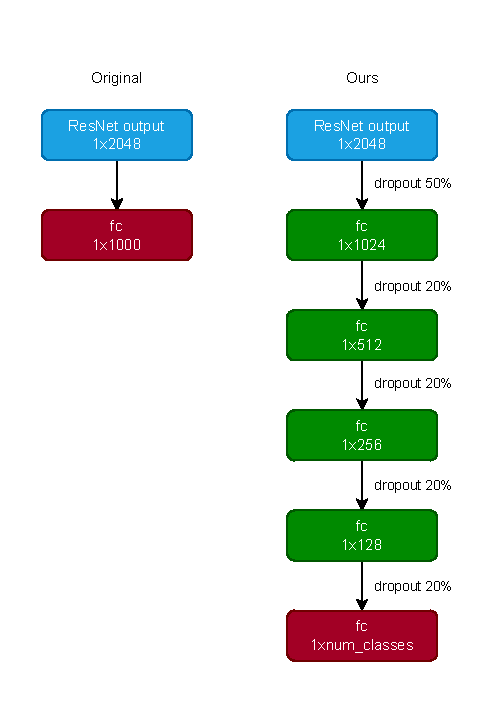
\includegraphics[width=0.6\textwidth]{figures/resnet_funnel.pdf}
      \caption{Our ResNet-50 architecture with a funnel layer for classification.
            Blue blocks represent the input from the ResNet-50 architecture,
            red blocks represent the final output layer,
            and green blocks represent our new funnel layers.}
      \label{fig:resnet_funnel}
\end{figure}

\subsubsection{Training Procedure}

In our initial training runs,
we observe severe overfitting on the training data as can be seen in Figure~\ref{fig:overfitting}.
To mitigate this, we apply several regularisation techniques:
\begin{itemize}
      \item \textbf{Dropout}~\cite{hinton_improving_2012}:
            As can be seen in Figure~\ref{fig:resnet_funnel},
            our fully connected layers contain dropout layers between them at rates of 0.5 and 0.2.
            Dropout is a regularisation technique that randomly sets a fraction of the input units to zero during training,
            which reinforces the model to learn more robust features and thereby reduces overfitting.
      \item \textbf{Data Augmentation}:
            We apply data augmentation techniques to our training data,
            such as random cropping, horizontal flipping, random erasing, and color jittering.
            These techniques artificially increase the size of our training dataset
            and help the model to generalise better by exposing it to a wider variety of input data.
\end{itemize}

\begin{figure}[ht]
      \centering
      \scalebox{0.6}{%% Creator: Matplotlib, PGF backend
%%
%% To include the figure in your LaTeX document, write
%%   \input{<filename>.pgf}
%%
%% Make sure the required packages are loaded in your preamble
%%   \usepackage{pgf}
%%
%% Also ensure that all the required font packages are loaded; for instance,
%% the lmodern package is sometimes necessary when using math font.
%%   \usepackage{lmodern}
%%
%% Figures using additional raster images can only be included by \input if
%% they are in the same directory as the main LaTeX file. For loading figures
%% from other directories you can use the `import` package
%%   \usepackage{import}
%%
%% and then include the figures with
%%   \import{<path to file>}{<filename>.pgf}
%%
%% Matplotlib used the following preamble
%%   \def\mathdefault#1{#1}
%%   \everymath=\expandafter{\the\everymath\displaystyle}
%%   \IfFileExists{scrextend.sty}{
%%     \usepackage[fontsize=11.000000pt]{scrextend}
%%   }{
%%     \renewcommand{\normalsize}{\fontsize{11.000000}{13.200000}\selectfont}
%%     \normalsize
%%   }
%%   
%%   \ifdefined\pdftexversion\else  % non-pdftex case.
%%     \usepackage{fontspec}
%%     \setmainfont{DejaVuSerif.ttf}[Path=\detokenize{/home/sentinel/.conda/envs/master-thesis/lib/python3.13/site-packages/matplotlib/mpl-data/fonts/ttf/}]
%%     \setsansfont{DejaVuSans.ttf}[Path=\detokenize{/home/sentinel/.conda/envs/master-thesis/lib/python3.13/site-packages/matplotlib/mpl-data/fonts/ttf/}]
%%     \setmonofont{DejaVuSansMono.ttf}[Path=\detokenize{/home/sentinel/.conda/envs/master-thesis/lib/python3.13/site-packages/matplotlib/mpl-data/fonts/ttf/}]
%%   \fi
%%   \makeatletter\@ifpackageloaded{underscore}{}{\usepackage[strings]{underscore}}\makeatother
%%
\begingroup%
\makeatletter%
\begin{pgfpicture}%
\pgfpathrectangle{\pgfpointorigin}{\pgfqpoint{5.344961in}{3.951110in}}%
\pgfusepath{use as bounding box, clip}%
\begin{pgfscope}%
\pgfsetbuttcap%
\pgfsetmiterjoin%
\definecolor{currentfill}{rgb}{1.000000,1.000000,1.000000}%
\pgfsetfillcolor{currentfill}%
\pgfsetlinewidth{0.000000pt}%
\definecolor{currentstroke}{rgb}{1.000000,1.000000,1.000000}%
\pgfsetstrokecolor{currentstroke}%
\pgfsetdash{}{0pt}%
\pgfpathmoveto{\pgfqpoint{0.000000in}{0.000000in}}%
\pgfpathlineto{\pgfqpoint{5.344961in}{0.000000in}}%
\pgfpathlineto{\pgfqpoint{5.344961in}{3.951110in}}%
\pgfpathlineto{\pgfqpoint{0.000000in}{3.951110in}}%
\pgfpathlineto{\pgfqpoint{0.000000in}{0.000000in}}%
\pgfpathclose%
\pgfusepath{fill}%
\end{pgfscope}%
\begin{pgfscope}%
\pgfsetbuttcap%
\pgfsetmiterjoin%
\definecolor{currentfill}{rgb}{1.000000,1.000000,1.000000}%
\pgfsetfillcolor{currentfill}%
\pgfsetlinewidth{0.000000pt}%
\definecolor{currentstroke}{rgb}{0.000000,0.000000,0.000000}%
\pgfsetstrokecolor{currentstroke}%
\pgfsetstrokeopacity{0.000000}%
\pgfsetdash{}{0pt}%
\pgfpathmoveto{\pgfqpoint{0.594961in}{0.548486in}}%
\pgfpathlineto{\pgfqpoint{5.244961in}{0.548486in}}%
\pgfpathlineto{\pgfqpoint{5.244961in}{3.628486in}}%
\pgfpathlineto{\pgfqpoint{0.594961in}{3.628486in}}%
\pgfpathlineto{\pgfqpoint{0.594961in}{0.548486in}}%
\pgfpathclose%
\pgfusepath{fill}%
\end{pgfscope}%
\begin{pgfscope}%
\pgfsetbuttcap%
\pgfsetroundjoin%
\definecolor{currentfill}{rgb}{0.000000,0.000000,0.000000}%
\pgfsetfillcolor{currentfill}%
\pgfsetlinewidth{0.803000pt}%
\definecolor{currentstroke}{rgb}{0.000000,0.000000,0.000000}%
\pgfsetstrokecolor{currentstroke}%
\pgfsetdash{}{0pt}%
\pgfsys@defobject{currentmarker}{\pgfqpoint{0.000000in}{-0.048611in}}{\pgfqpoint{0.000000in}{0.000000in}}{%
\pgfpathmoveto{\pgfqpoint{0.000000in}{0.000000in}}%
\pgfpathlineto{\pgfqpoint{0.000000in}{-0.048611in}}%
\pgfusepath{stroke,fill}%
}%
\begin{pgfscope}%
\pgfsys@transformshift{0.799717in}{0.548486in}%
\pgfsys@useobject{currentmarker}{}%
\end{pgfscope}%
\end{pgfscope}%
\begin{pgfscope}%
\definecolor{textcolor}{rgb}{0.000000,0.000000,0.000000}%
\pgfsetstrokecolor{textcolor}%
\pgfsetfillcolor{textcolor}%
\pgftext[x=0.799717in,y=0.451264in,,top]{\color{textcolor}{\fontsize{11.000000}{13.200000}\selectfont\catcode`\^=\active\def^{\ifmmode\sp\else\^{}\fi}\catcode`\%=\active\def%{\%}$\mathdefault{0}$}}%
\end{pgfscope}%
\begin{pgfscope}%
\pgfsetbuttcap%
\pgfsetroundjoin%
\definecolor{currentfill}{rgb}{0.000000,0.000000,0.000000}%
\pgfsetfillcolor{currentfill}%
\pgfsetlinewidth{0.803000pt}%
\definecolor{currentstroke}{rgb}{0.000000,0.000000,0.000000}%
\pgfsetstrokecolor{currentstroke}%
\pgfsetdash{}{0pt}%
\pgfsys@defobject{currentmarker}{\pgfqpoint{0.000000in}{-0.048611in}}{\pgfqpoint{0.000000in}{0.000000in}}{%
\pgfpathmoveto{\pgfqpoint{0.000000in}{0.000000in}}%
\pgfpathlineto{\pgfqpoint{0.000000in}{-0.048611in}}%
\pgfusepath{stroke,fill}%
}%
\begin{pgfscope}%
\pgfsys@transformshift{1.473924in}{0.548486in}%
\pgfsys@useobject{currentmarker}{}%
\end{pgfscope}%
\end{pgfscope}%
\begin{pgfscope}%
\definecolor{textcolor}{rgb}{0.000000,0.000000,0.000000}%
\pgfsetstrokecolor{textcolor}%
\pgfsetfillcolor{textcolor}%
\pgftext[x=1.473924in,y=0.451264in,,top]{\color{textcolor}{\fontsize{11.000000}{13.200000}\selectfont\catcode`\^=\active\def^{\ifmmode\sp\else\^{}\fi}\catcode`\%=\active\def%{\%}$\mathdefault{5000}$}}%
\end{pgfscope}%
\begin{pgfscope}%
\pgfsetbuttcap%
\pgfsetroundjoin%
\definecolor{currentfill}{rgb}{0.000000,0.000000,0.000000}%
\pgfsetfillcolor{currentfill}%
\pgfsetlinewidth{0.803000pt}%
\definecolor{currentstroke}{rgb}{0.000000,0.000000,0.000000}%
\pgfsetstrokecolor{currentstroke}%
\pgfsetdash{}{0pt}%
\pgfsys@defobject{currentmarker}{\pgfqpoint{0.000000in}{-0.048611in}}{\pgfqpoint{0.000000in}{0.000000in}}{%
\pgfpathmoveto{\pgfqpoint{0.000000in}{0.000000in}}%
\pgfpathlineto{\pgfqpoint{0.000000in}{-0.048611in}}%
\pgfusepath{stroke,fill}%
}%
\begin{pgfscope}%
\pgfsys@transformshift{2.148130in}{0.548486in}%
\pgfsys@useobject{currentmarker}{}%
\end{pgfscope}%
\end{pgfscope}%
\begin{pgfscope}%
\definecolor{textcolor}{rgb}{0.000000,0.000000,0.000000}%
\pgfsetstrokecolor{textcolor}%
\pgfsetfillcolor{textcolor}%
\pgftext[x=2.148130in,y=0.451264in,,top]{\color{textcolor}{\fontsize{11.000000}{13.200000}\selectfont\catcode`\^=\active\def^{\ifmmode\sp\else\^{}\fi}\catcode`\%=\active\def%{\%}$\mathdefault{10000}$}}%
\end{pgfscope}%
\begin{pgfscope}%
\pgfsetbuttcap%
\pgfsetroundjoin%
\definecolor{currentfill}{rgb}{0.000000,0.000000,0.000000}%
\pgfsetfillcolor{currentfill}%
\pgfsetlinewidth{0.803000pt}%
\definecolor{currentstroke}{rgb}{0.000000,0.000000,0.000000}%
\pgfsetstrokecolor{currentstroke}%
\pgfsetdash{}{0pt}%
\pgfsys@defobject{currentmarker}{\pgfqpoint{0.000000in}{-0.048611in}}{\pgfqpoint{0.000000in}{0.000000in}}{%
\pgfpathmoveto{\pgfqpoint{0.000000in}{0.000000in}}%
\pgfpathlineto{\pgfqpoint{0.000000in}{-0.048611in}}%
\pgfusepath{stroke,fill}%
}%
\begin{pgfscope}%
\pgfsys@transformshift{2.822336in}{0.548486in}%
\pgfsys@useobject{currentmarker}{}%
\end{pgfscope}%
\end{pgfscope}%
\begin{pgfscope}%
\definecolor{textcolor}{rgb}{0.000000,0.000000,0.000000}%
\pgfsetstrokecolor{textcolor}%
\pgfsetfillcolor{textcolor}%
\pgftext[x=2.822336in,y=0.451264in,,top]{\color{textcolor}{\fontsize{11.000000}{13.200000}\selectfont\catcode`\^=\active\def^{\ifmmode\sp\else\^{}\fi}\catcode`\%=\active\def%{\%}$\mathdefault{15000}$}}%
\end{pgfscope}%
\begin{pgfscope}%
\pgfsetbuttcap%
\pgfsetroundjoin%
\definecolor{currentfill}{rgb}{0.000000,0.000000,0.000000}%
\pgfsetfillcolor{currentfill}%
\pgfsetlinewidth{0.803000pt}%
\definecolor{currentstroke}{rgb}{0.000000,0.000000,0.000000}%
\pgfsetstrokecolor{currentstroke}%
\pgfsetdash{}{0pt}%
\pgfsys@defobject{currentmarker}{\pgfqpoint{0.000000in}{-0.048611in}}{\pgfqpoint{0.000000in}{0.000000in}}{%
\pgfpathmoveto{\pgfqpoint{0.000000in}{0.000000in}}%
\pgfpathlineto{\pgfqpoint{0.000000in}{-0.048611in}}%
\pgfusepath{stroke,fill}%
}%
\begin{pgfscope}%
\pgfsys@transformshift{3.496542in}{0.548486in}%
\pgfsys@useobject{currentmarker}{}%
\end{pgfscope}%
\end{pgfscope}%
\begin{pgfscope}%
\definecolor{textcolor}{rgb}{0.000000,0.000000,0.000000}%
\pgfsetstrokecolor{textcolor}%
\pgfsetfillcolor{textcolor}%
\pgftext[x=3.496542in,y=0.451264in,,top]{\color{textcolor}{\fontsize{11.000000}{13.200000}\selectfont\catcode`\^=\active\def^{\ifmmode\sp\else\^{}\fi}\catcode`\%=\active\def%{\%}$\mathdefault{20000}$}}%
\end{pgfscope}%
\begin{pgfscope}%
\pgfsetbuttcap%
\pgfsetroundjoin%
\definecolor{currentfill}{rgb}{0.000000,0.000000,0.000000}%
\pgfsetfillcolor{currentfill}%
\pgfsetlinewidth{0.803000pt}%
\definecolor{currentstroke}{rgb}{0.000000,0.000000,0.000000}%
\pgfsetstrokecolor{currentstroke}%
\pgfsetdash{}{0pt}%
\pgfsys@defobject{currentmarker}{\pgfqpoint{0.000000in}{-0.048611in}}{\pgfqpoint{0.000000in}{0.000000in}}{%
\pgfpathmoveto{\pgfqpoint{0.000000in}{0.000000in}}%
\pgfpathlineto{\pgfqpoint{0.000000in}{-0.048611in}}%
\pgfusepath{stroke,fill}%
}%
\begin{pgfscope}%
\pgfsys@transformshift{4.170748in}{0.548486in}%
\pgfsys@useobject{currentmarker}{}%
\end{pgfscope}%
\end{pgfscope}%
\begin{pgfscope}%
\definecolor{textcolor}{rgb}{0.000000,0.000000,0.000000}%
\pgfsetstrokecolor{textcolor}%
\pgfsetfillcolor{textcolor}%
\pgftext[x=4.170748in,y=0.451264in,,top]{\color{textcolor}{\fontsize{11.000000}{13.200000}\selectfont\catcode`\^=\active\def^{\ifmmode\sp\else\^{}\fi}\catcode`\%=\active\def%{\%}$\mathdefault{25000}$}}%
\end{pgfscope}%
\begin{pgfscope}%
\pgfsetbuttcap%
\pgfsetroundjoin%
\definecolor{currentfill}{rgb}{0.000000,0.000000,0.000000}%
\pgfsetfillcolor{currentfill}%
\pgfsetlinewidth{0.803000pt}%
\definecolor{currentstroke}{rgb}{0.000000,0.000000,0.000000}%
\pgfsetstrokecolor{currentstroke}%
\pgfsetdash{}{0pt}%
\pgfsys@defobject{currentmarker}{\pgfqpoint{0.000000in}{-0.048611in}}{\pgfqpoint{0.000000in}{0.000000in}}{%
\pgfpathmoveto{\pgfqpoint{0.000000in}{0.000000in}}%
\pgfpathlineto{\pgfqpoint{0.000000in}{-0.048611in}}%
\pgfusepath{stroke,fill}%
}%
\begin{pgfscope}%
\pgfsys@transformshift{4.844954in}{0.548486in}%
\pgfsys@useobject{currentmarker}{}%
\end{pgfscope}%
\end{pgfscope}%
\begin{pgfscope}%
\definecolor{textcolor}{rgb}{0.000000,0.000000,0.000000}%
\pgfsetstrokecolor{textcolor}%
\pgfsetfillcolor{textcolor}%
\pgftext[x=4.844954in,y=0.451264in,,top]{\color{textcolor}{\fontsize{11.000000}{13.200000}\selectfont\catcode`\^=\active\def^{\ifmmode\sp\else\^{}\fi}\catcode`\%=\active\def%{\%}$\mathdefault{30000}$}}%
\end{pgfscope}%
\begin{pgfscope}%
\definecolor{textcolor}{rgb}{0.000000,0.000000,0.000000}%
\pgfsetstrokecolor{textcolor}%
\pgfsetfillcolor{textcolor}%
\pgftext[x=2.919961in,y=0.247854in,,top]{\color{textcolor}{\fontsize{11.000000}{13.200000}\selectfont\catcode`\^=\active\def^{\ifmmode\sp\else\^{}\fi}\catcode`\%=\active\def%{\%}Steps}}%
\end{pgfscope}%
\begin{pgfscope}%
\pgfsetbuttcap%
\pgfsetroundjoin%
\definecolor{currentfill}{rgb}{0.000000,0.000000,0.000000}%
\pgfsetfillcolor{currentfill}%
\pgfsetlinewidth{0.803000pt}%
\definecolor{currentstroke}{rgb}{0.000000,0.000000,0.000000}%
\pgfsetstrokecolor{currentstroke}%
\pgfsetdash{}{0pt}%
\pgfsys@defobject{currentmarker}{\pgfqpoint{-0.048611in}{0.000000in}}{\pgfqpoint{-0.000000in}{0.000000in}}{%
\pgfpathmoveto{\pgfqpoint{-0.000000in}{0.000000in}}%
\pgfpathlineto{\pgfqpoint{-0.048611in}{0.000000in}}%
\pgfusepath{stroke,fill}%
}%
\begin{pgfscope}%
\pgfsys@transformshift{0.594961in}{0.688486in}%
\pgfsys@useobject{currentmarker}{}%
\end{pgfscope}%
\end{pgfscope}%
\begin{pgfscope}%
\definecolor{textcolor}{rgb}{0.000000,0.000000,0.000000}%
\pgfsetstrokecolor{textcolor}%
\pgfsetfillcolor{textcolor}%
\pgftext[x=0.303410in, y=0.630449in, left, base]{\color{textcolor}{\fontsize{11.000000}{13.200000}\selectfont\catcode`\^=\active\def^{\ifmmode\sp\else\^{}\fi}\catcode`\%=\active\def%{\%}$\mathdefault{0.0}$}}%
\end{pgfscope}%
\begin{pgfscope}%
\pgfsetbuttcap%
\pgfsetroundjoin%
\definecolor{currentfill}{rgb}{0.000000,0.000000,0.000000}%
\pgfsetfillcolor{currentfill}%
\pgfsetlinewidth{0.803000pt}%
\definecolor{currentstroke}{rgb}{0.000000,0.000000,0.000000}%
\pgfsetstrokecolor{currentstroke}%
\pgfsetdash{}{0pt}%
\pgfsys@defobject{currentmarker}{\pgfqpoint{-0.048611in}{0.000000in}}{\pgfqpoint{-0.000000in}{0.000000in}}{%
\pgfpathmoveto{\pgfqpoint{-0.000000in}{0.000000in}}%
\pgfpathlineto{\pgfqpoint{-0.048611in}{0.000000in}}%
\pgfusepath{stroke,fill}%
}%
\begin{pgfscope}%
\pgfsys@transformshift{0.594961in}{1.248486in}%
\pgfsys@useobject{currentmarker}{}%
\end{pgfscope}%
\end{pgfscope}%
\begin{pgfscope}%
\definecolor{textcolor}{rgb}{0.000000,0.000000,0.000000}%
\pgfsetstrokecolor{textcolor}%
\pgfsetfillcolor{textcolor}%
\pgftext[x=0.303410in, y=1.190449in, left, base]{\color{textcolor}{\fontsize{11.000000}{13.200000}\selectfont\catcode`\^=\active\def^{\ifmmode\sp\else\^{}\fi}\catcode`\%=\active\def%{\%}$\mathdefault{0.2}$}}%
\end{pgfscope}%
\begin{pgfscope}%
\pgfsetbuttcap%
\pgfsetroundjoin%
\definecolor{currentfill}{rgb}{0.000000,0.000000,0.000000}%
\pgfsetfillcolor{currentfill}%
\pgfsetlinewidth{0.803000pt}%
\definecolor{currentstroke}{rgb}{0.000000,0.000000,0.000000}%
\pgfsetstrokecolor{currentstroke}%
\pgfsetdash{}{0pt}%
\pgfsys@defobject{currentmarker}{\pgfqpoint{-0.048611in}{0.000000in}}{\pgfqpoint{-0.000000in}{0.000000in}}{%
\pgfpathmoveto{\pgfqpoint{-0.000000in}{0.000000in}}%
\pgfpathlineto{\pgfqpoint{-0.048611in}{0.000000in}}%
\pgfusepath{stroke,fill}%
}%
\begin{pgfscope}%
\pgfsys@transformshift{0.594961in}{1.808486in}%
\pgfsys@useobject{currentmarker}{}%
\end{pgfscope}%
\end{pgfscope}%
\begin{pgfscope}%
\definecolor{textcolor}{rgb}{0.000000,0.000000,0.000000}%
\pgfsetstrokecolor{textcolor}%
\pgfsetfillcolor{textcolor}%
\pgftext[x=0.303410in, y=1.750449in, left, base]{\color{textcolor}{\fontsize{11.000000}{13.200000}\selectfont\catcode`\^=\active\def^{\ifmmode\sp\else\^{}\fi}\catcode`\%=\active\def%{\%}$\mathdefault{0.4}$}}%
\end{pgfscope}%
\begin{pgfscope}%
\pgfsetbuttcap%
\pgfsetroundjoin%
\definecolor{currentfill}{rgb}{0.000000,0.000000,0.000000}%
\pgfsetfillcolor{currentfill}%
\pgfsetlinewidth{0.803000pt}%
\definecolor{currentstroke}{rgb}{0.000000,0.000000,0.000000}%
\pgfsetstrokecolor{currentstroke}%
\pgfsetdash{}{0pt}%
\pgfsys@defobject{currentmarker}{\pgfqpoint{-0.048611in}{0.000000in}}{\pgfqpoint{-0.000000in}{0.000000in}}{%
\pgfpathmoveto{\pgfqpoint{-0.000000in}{0.000000in}}%
\pgfpathlineto{\pgfqpoint{-0.048611in}{0.000000in}}%
\pgfusepath{stroke,fill}%
}%
\begin{pgfscope}%
\pgfsys@transformshift{0.594961in}{2.368486in}%
\pgfsys@useobject{currentmarker}{}%
\end{pgfscope}%
\end{pgfscope}%
\begin{pgfscope}%
\definecolor{textcolor}{rgb}{0.000000,0.000000,0.000000}%
\pgfsetstrokecolor{textcolor}%
\pgfsetfillcolor{textcolor}%
\pgftext[x=0.303410in, y=2.310449in, left, base]{\color{textcolor}{\fontsize{11.000000}{13.200000}\selectfont\catcode`\^=\active\def^{\ifmmode\sp\else\^{}\fi}\catcode`\%=\active\def%{\%}$\mathdefault{0.6}$}}%
\end{pgfscope}%
\begin{pgfscope}%
\pgfsetbuttcap%
\pgfsetroundjoin%
\definecolor{currentfill}{rgb}{0.000000,0.000000,0.000000}%
\pgfsetfillcolor{currentfill}%
\pgfsetlinewidth{0.803000pt}%
\definecolor{currentstroke}{rgb}{0.000000,0.000000,0.000000}%
\pgfsetstrokecolor{currentstroke}%
\pgfsetdash{}{0pt}%
\pgfsys@defobject{currentmarker}{\pgfqpoint{-0.048611in}{0.000000in}}{\pgfqpoint{-0.000000in}{0.000000in}}{%
\pgfpathmoveto{\pgfqpoint{-0.000000in}{0.000000in}}%
\pgfpathlineto{\pgfqpoint{-0.048611in}{0.000000in}}%
\pgfusepath{stroke,fill}%
}%
\begin{pgfscope}%
\pgfsys@transformshift{0.594961in}{2.928486in}%
\pgfsys@useobject{currentmarker}{}%
\end{pgfscope}%
\end{pgfscope}%
\begin{pgfscope}%
\definecolor{textcolor}{rgb}{0.000000,0.000000,0.000000}%
\pgfsetstrokecolor{textcolor}%
\pgfsetfillcolor{textcolor}%
\pgftext[x=0.303410in, y=2.870449in, left, base]{\color{textcolor}{\fontsize{11.000000}{13.200000}\selectfont\catcode`\^=\active\def^{\ifmmode\sp\else\^{}\fi}\catcode`\%=\active\def%{\%}$\mathdefault{0.8}$}}%
\end{pgfscope}%
\begin{pgfscope}%
\pgfsetbuttcap%
\pgfsetroundjoin%
\definecolor{currentfill}{rgb}{0.000000,0.000000,0.000000}%
\pgfsetfillcolor{currentfill}%
\pgfsetlinewidth{0.803000pt}%
\definecolor{currentstroke}{rgb}{0.000000,0.000000,0.000000}%
\pgfsetstrokecolor{currentstroke}%
\pgfsetdash{}{0pt}%
\pgfsys@defobject{currentmarker}{\pgfqpoint{-0.048611in}{0.000000in}}{\pgfqpoint{-0.000000in}{0.000000in}}{%
\pgfpathmoveto{\pgfqpoint{-0.000000in}{0.000000in}}%
\pgfpathlineto{\pgfqpoint{-0.048611in}{0.000000in}}%
\pgfusepath{stroke,fill}%
}%
\begin{pgfscope}%
\pgfsys@transformshift{0.594961in}{3.488486in}%
\pgfsys@useobject{currentmarker}{}%
\end{pgfscope}%
\end{pgfscope}%
\begin{pgfscope}%
\definecolor{textcolor}{rgb}{0.000000,0.000000,0.000000}%
\pgfsetstrokecolor{textcolor}%
\pgfsetfillcolor{textcolor}%
\pgftext[x=0.303410in, y=3.430449in, left, base]{\color{textcolor}{\fontsize{11.000000}{13.200000}\selectfont\catcode`\^=\active\def^{\ifmmode\sp\else\^{}\fi}\catcode`\%=\active\def%{\%}$\mathdefault{1.0}$}}%
\end{pgfscope}%
\begin{pgfscope}%
\definecolor{textcolor}{rgb}{0.000000,0.000000,0.000000}%
\pgfsetstrokecolor{textcolor}%
\pgfsetfillcolor{textcolor}%
\pgftext[x=0.247854in,y=2.088486in,,bottom,rotate=90.000000]{\color{textcolor}{\fontsize{11.000000}{13.200000}\selectfont\catcode`\^=\active\def^{\ifmmode\sp\else\^{}\fi}\catcode`\%=\active\def%{\%}Accuracy}}%
\end{pgfscope}%
\begin{pgfscope}%
\pgfpathrectangle{\pgfqpoint{0.594961in}{0.548486in}}{\pgfqpoint{4.650000in}{3.080000in}}%
\pgfusepath{clip}%
\pgfsetrectcap%
\pgfsetroundjoin%
\pgfsetlinewidth{1.505625pt}%
\definecolor{currentstroke}{rgb}{0.121569,0.466667,0.705882}%
\pgfsetstrokecolor{currentstroke}%
\pgfsetdash{}{0pt}%
\pgfpathmoveto{\pgfqpoint{0.806325in}{0.688486in}}%
\pgfpathlineto{\pgfqpoint{0.813067in}{0.754111in}}%
\pgfpathlineto{\pgfqpoint{0.819809in}{0.732236in}}%
\pgfpathlineto{\pgfqpoint{0.826551in}{0.765049in}}%
\pgfpathlineto{\pgfqpoint{0.833293in}{0.699424in}}%
\pgfpathlineto{\pgfqpoint{0.840035in}{0.721299in}}%
\pgfpathlineto{\pgfqpoint{0.846777in}{0.721299in}}%
\pgfpathlineto{\pgfqpoint{0.853519in}{0.699424in}}%
\pgfpathlineto{\pgfqpoint{0.860261in}{0.754111in}}%
\pgfpathlineto{\pgfqpoint{0.867003in}{0.721299in}}%
\pgfpathlineto{\pgfqpoint{0.873745in}{0.754111in}}%
\pgfpathlineto{\pgfqpoint{0.880487in}{0.743174in}}%
\pgfpathlineto{\pgfqpoint{0.887229in}{0.830674in}}%
\pgfpathlineto{\pgfqpoint{0.893971in}{0.797861in}}%
\pgfpathlineto{\pgfqpoint{0.900713in}{0.775986in}}%
\pgfpathlineto{\pgfqpoint{0.907456in}{0.797861in}}%
\pgfpathlineto{\pgfqpoint{0.914198in}{0.841611in}}%
\pgfpathlineto{\pgfqpoint{0.920940in}{0.819736in}}%
\pgfpathlineto{\pgfqpoint{0.927682in}{0.819736in}}%
\pgfpathlineto{\pgfqpoint{0.934424in}{0.885361in}}%
\pgfpathlineto{\pgfqpoint{0.941166in}{0.808799in}}%
\pgfpathlineto{\pgfqpoint{0.947908in}{0.797861in}}%
\pgfpathlineto{\pgfqpoint{0.954650in}{0.819736in}}%
\pgfpathlineto{\pgfqpoint{0.968134in}{0.797861in}}%
\pgfpathlineto{\pgfqpoint{0.974876in}{0.797861in}}%
\pgfpathlineto{\pgfqpoint{0.981618in}{0.852549in}}%
\pgfpathlineto{\pgfqpoint{0.988360in}{0.808799in}}%
\pgfpathlineto{\pgfqpoint{0.995102in}{0.863486in}}%
\pgfpathlineto{\pgfqpoint{1.001844in}{0.841611in}}%
\pgfpathlineto{\pgfqpoint{1.008586in}{0.940049in}}%
\pgfpathlineto{\pgfqpoint{1.015329in}{0.940049in}}%
\pgfpathlineto{\pgfqpoint{1.022071in}{1.016611in}}%
\pgfpathlineto{\pgfqpoint{1.028813in}{0.961924in}}%
\pgfpathlineto{\pgfqpoint{1.035555in}{0.950986in}}%
\pgfpathlineto{\pgfqpoint{1.042297in}{0.994736in}}%
\pgfpathlineto{\pgfqpoint{1.049039in}{0.940049in}}%
\pgfpathlineto{\pgfqpoint{1.055781in}{1.049424in}}%
\pgfpathlineto{\pgfqpoint{1.062523in}{1.060361in}}%
\pgfpathlineto{\pgfqpoint{1.069265in}{1.104111in}}%
\pgfpathlineto{\pgfqpoint{1.076007in}{0.950986in}}%
\pgfpathlineto{\pgfqpoint{1.082749in}{1.016611in}}%
\pgfpathlineto{\pgfqpoint{1.089491in}{1.071299in}}%
\pgfpathlineto{\pgfqpoint{1.096233in}{1.093174in}}%
\pgfpathlineto{\pgfqpoint{1.102975in}{1.180674in}}%
\pgfpathlineto{\pgfqpoint{1.109717in}{1.060361in}}%
\pgfpathlineto{\pgfqpoint{1.116459in}{1.136924in}}%
\pgfpathlineto{\pgfqpoint{1.129944in}{1.093174in}}%
\pgfpathlineto{\pgfqpoint{1.136686in}{1.093174in}}%
\pgfpathlineto{\pgfqpoint{1.143428in}{1.027549in}}%
\pgfpathlineto{\pgfqpoint{1.150170in}{1.136924in}}%
\pgfpathlineto{\pgfqpoint{1.156912in}{0.841611in}}%
\pgfpathlineto{\pgfqpoint{1.163654in}{1.125986in}}%
\pgfpathlineto{\pgfqpoint{1.170396in}{1.071299in}}%
\pgfpathlineto{\pgfqpoint{1.177138in}{1.213486in}}%
\pgfpathlineto{\pgfqpoint{1.183880in}{1.202549in}}%
\pgfpathlineto{\pgfqpoint{1.190622in}{1.300986in}}%
\pgfpathlineto{\pgfqpoint{1.197364in}{1.213486in}}%
\pgfpathlineto{\pgfqpoint{1.204106in}{1.224424in}}%
\pgfpathlineto{\pgfqpoint{1.210848in}{1.344736in}}%
\pgfpathlineto{\pgfqpoint{1.217590in}{1.377549in}}%
\pgfpathlineto{\pgfqpoint{1.224332in}{1.333799in}}%
\pgfpathlineto{\pgfqpoint{1.231074in}{1.443174in}}%
\pgfpathlineto{\pgfqpoint{1.237817in}{1.377549in}}%
\pgfpathlineto{\pgfqpoint{1.244559in}{1.355674in}}%
\pgfpathlineto{\pgfqpoint{1.251301in}{1.410361in}}%
\pgfpathlineto{\pgfqpoint{1.258043in}{1.388486in}}%
\pgfpathlineto{\pgfqpoint{1.264785in}{1.410361in}}%
\pgfpathlineto{\pgfqpoint{1.271527in}{1.486924in}}%
\pgfpathlineto{\pgfqpoint{1.278269in}{1.443174in}}%
\pgfpathlineto{\pgfqpoint{1.285011in}{1.574424in}}%
\pgfpathlineto{\pgfqpoint{1.291753in}{1.519736in}}%
\pgfpathlineto{\pgfqpoint{1.298495in}{1.629111in}}%
\pgfpathlineto{\pgfqpoint{1.305237in}{1.497861in}}%
\pgfpathlineto{\pgfqpoint{1.311979in}{1.618174in}}%
\pgfpathlineto{\pgfqpoint{1.318721in}{1.661924in}}%
\pgfpathlineto{\pgfqpoint{1.325463in}{1.475986in}}%
\pgfpathlineto{\pgfqpoint{1.332205in}{1.661924in}}%
\pgfpathlineto{\pgfqpoint{1.338947in}{1.530674in}}%
\pgfpathlineto{\pgfqpoint{1.345690in}{1.596299in}}%
\pgfpathlineto{\pgfqpoint{1.352432in}{1.574424in}}%
\pgfpathlineto{\pgfqpoint{1.359174in}{1.607236in}}%
\pgfpathlineto{\pgfqpoint{1.365916in}{1.705674in}}%
\pgfpathlineto{\pgfqpoint{1.372658in}{1.782236in}}%
\pgfpathlineto{\pgfqpoint{1.379400in}{1.541611in}}%
\pgfpathlineto{\pgfqpoint{1.392884in}{1.716611in}}%
\pgfpathlineto{\pgfqpoint{1.399626in}{1.771299in}}%
\pgfpathlineto{\pgfqpoint{1.406368in}{1.738486in}}%
\pgfpathlineto{\pgfqpoint{1.413110in}{1.596299in}}%
\pgfpathlineto{\pgfqpoint{1.419852in}{1.650986in}}%
\pgfpathlineto{\pgfqpoint{1.426594in}{1.880674in}}%
\pgfpathlineto{\pgfqpoint{1.433336in}{1.771299in}}%
\pgfpathlineto{\pgfqpoint{1.440078in}{1.858799in}}%
\pgfpathlineto{\pgfqpoint{1.446820in}{1.596299in}}%
\pgfpathlineto{\pgfqpoint{1.453563in}{1.705674in}}%
\pgfpathlineto{\pgfqpoint{1.467047in}{1.640049in}}%
\pgfpathlineto{\pgfqpoint{1.473789in}{1.902549in}}%
\pgfpathlineto{\pgfqpoint{1.480531in}{2.088486in}}%
\pgfpathlineto{\pgfqpoint{1.487273in}{1.869736in}}%
\pgfpathlineto{\pgfqpoint{1.494015in}{1.869736in}}%
\pgfpathlineto{\pgfqpoint{1.500757in}{1.847861in}}%
\pgfpathlineto{\pgfqpoint{1.507499in}{1.836924in}}%
\pgfpathlineto{\pgfqpoint{1.514241in}{2.077549in}}%
\pgfpathlineto{\pgfqpoint{1.520983in}{1.869736in}}%
\pgfpathlineto{\pgfqpoint{1.527725in}{1.979111in}}%
\pgfpathlineto{\pgfqpoint{1.534467in}{2.000986in}}%
\pgfpathlineto{\pgfqpoint{1.541209in}{2.044736in}}%
\pgfpathlineto{\pgfqpoint{1.547951in}{1.858799in}}%
\pgfpathlineto{\pgfqpoint{1.554693in}{1.891611in}}%
\pgfpathlineto{\pgfqpoint{1.561436in}{2.077549in}}%
\pgfpathlineto{\pgfqpoint{1.568178in}{1.990049in}}%
\pgfpathlineto{\pgfqpoint{1.574920in}{1.836924in}}%
\pgfpathlineto{\pgfqpoint{1.581662in}{1.541611in}}%
\pgfpathlineto{\pgfqpoint{1.588404in}{1.935361in}}%
\pgfpathlineto{\pgfqpoint{1.595146in}{1.946299in}}%
\pgfpathlineto{\pgfqpoint{1.601888in}{2.066611in}}%
\pgfpathlineto{\pgfqpoint{1.608630in}{1.935361in}}%
\pgfpathlineto{\pgfqpoint{1.615372in}{1.902549in}}%
\pgfpathlineto{\pgfqpoint{1.622114in}{2.219736in}}%
\pgfpathlineto{\pgfqpoint{1.628856in}{2.055674in}}%
\pgfpathlineto{\pgfqpoint{1.635598in}{2.066611in}}%
\pgfpathlineto{\pgfqpoint{1.642340in}{2.099424in}}%
\pgfpathlineto{\pgfqpoint{1.649082in}{2.263486in}}%
\pgfpathlineto{\pgfqpoint{1.655824in}{2.110361in}}%
\pgfpathlineto{\pgfqpoint{1.662566in}{2.044736in}}%
\pgfpathlineto{\pgfqpoint{1.669309in}{2.175986in}}%
\pgfpathlineto{\pgfqpoint{1.676051in}{2.186924in}}%
\pgfpathlineto{\pgfqpoint{1.682793in}{2.186924in}}%
\pgfpathlineto{\pgfqpoint{1.689535in}{2.252549in}}%
\pgfpathlineto{\pgfqpoint{1.696277in}{2.132236in}}%
\pgfpathlineto{\pgfqpoint{1.703019in}{2.241611in}}%
\pgfpathlineto{\pgfqpoint{1.709761in}{2.022861in}}%
\pgfpathlineto{\pgfqpoint{1.716503in}{2.197861in}}%
\pgfpathlineto{\pgfqpoint{1.723245in}{2.099424in}}%
\pgfpathlineto{\pgfqpoint{1.729987in}{2.252549in}}%
\pgfpathlineto{\pgfqpoint{1.736729in}{2.121299in}}%
\pgfpathlineto{\pgfqpoint{1.743471in}{2.296299in}}%
\pgfpathlineto{\pgfqpoint{1.750213in}{2.165049in}}%
\pgfpathlineto{\pgfqpoint{1.763697in}{2.252549in}}%
\pgfpathlineto{\pgfqpoint{1.770439in}{2.219736in}}%
\pgfpathlineto{\pgfqpoint{1.777182in}{2.416611in}}%
\pgfpathlineto{\pgfqpoint{1.783924in}{2.208799in}}%
\pgfpathlineto{\pgfqpoint{1.790666in}{2.427549in}}%
\pgfpathlineto{\pgfqpoint{1.797408in}{2.296299in}}%
\pgfpathlineto{\pgfqpoint{1.804150in}{2.536924in}}%
\pgfpathlineto{\pgfqpoint{1.810892in}{2.383799in}}%
\pgfpathlineto{\pgfqpoint{1.817634in}{2.416611in}}%
\pgfpathlineto{\pgfqpoint{1.824376in}{2.219736in}}%
\pgfpathlineto{\pgfqpoint{1.831118in}{2.252549in}}%
\pgfpathlineto{\pgfqpoint{1.837860in}{2.329111in}}%
\pgfpathlineto{\pgfqpoint{1.844602in}{2.318174in}}%
\pgfpathlineto{\pgfqpoint{1.851344in}{2.536924in}}%
\pgfpathlineto{\pgfqpoint{1.858086in}{3.138486in}}%
\pgfpathlineto{\pgfqpoint{1.864828in}{2.394736in}}%
\pgfpathlineto{\pgfqpoint{1.871570in}{2.679111in}}%
\pgfpathlineto{\pgfqpoint{1.878312in}{2.613486in}}%
\pgfpathlineto{\pgfqpoint{1.885054in}{2.558799in}}%
\pgfpathlineto{\pgfqpoint{1.891797in}{2.449424in}}%
\pgfpathlineto{\pgfqpoint{1.898539in}{2.438486in}}%
\pgfpathlineto{\pgfqpoint{1.905281in}{2.624424in}}%
\pgfpathlineto{\pgfqpoint{1.912023in}{2.427549in}}%
\pgfpathlineto{\pgfqpoint{1.918765in}{2.493174in}}%
\pgfpathlineto{\pgfqpoint{1.925507in}{2.427549in}}%
\pgfpathlineto{\pgfqpoint{1.932249in}{2.449424in}}%
\pgfpathlineto{\pgfqpoint{1.938991in}{2.580674in}}%
\pgfpathlineto{\pgfqpoint{1.945733in}{2.536924in}}%
\pgfpathlineto{\pgfqpoint{1.952475in}{2.482236in}}%
\pgfpathlineto{\pgfqpoint{1.959217in}{2.493174in}}%
\pgfpathlineto{\pgfqpoint{1.965959in}{2.405674in}}%
\pgfpathlineto{\pgfqpoint{1.972701in}{2.504111in}}%
\pgfpathlineto{\pgfqpoint{1.979443in}{2.525986in}}%
\pgfpathlineto{\pgfqpoint{1.986185in}{2.525986in}}%
\pgfpathlineto{\pgfqpoint{1.992927in}{2.493174in}}%
\pgfpathlineto{\pgfqpoint{1.999670in}{2.613486in}}%
\pgfpathlineto{\pgfqpoint{2.006412in}{2.471299in}}%
\pgfpathlineto{\pgfqpoint{2.013154in}{2.515049in}}%
\pgfpathlineto{\pgfqpoint{2.019896in}{2.471299in}}%
\pgfpathlineto{\pgfqpoint{2.026638in}{2.624424in}}%
\pgfpathlineto{\pgfqpoint{2.033380in}{2.350986in}}%
\pgfpathlineto{\pgfqpoint{2.040122in}{2.525986in}}%
\pgfpathlineto{\pgfqpoint{2.046864in}{2.536924in}}%
\pgfpathlineto{\pgfqpoint{2.053606in}{2.635361in}}%
\pgfpathlineto{\pgfqpoint{2.060348in}{2.536924in}}%
\pgfpathlineto{\pgfqpoint{2.067090in}{2.602549in}}%
\pgfpathlineto{\pgfqpoint{2.073832in}{2.646299in}}%
\pgfpathlineto{\pgfqpoint{2.080574in}{2.952549in}}%
\pgfpathlineto{\pgfqpoint{2.087316in}{3.204111in}}%
\pgfpathlineto{\pgfqpoint{2.094058in}{3.061924in}}%
\pgfpathlineto{\pgfqpoint{2.100800in}{3.061924in}}%
\pgfpathlineto{\pgfqpoint{2.107543in}{3.204111in}}%
\pgfpathlineto{\pgfqpoint{2.114285in}{3.138486in}}%
\pgfpathlineto{\pgfqpoint{2.121027in}{3.225986in}}%
\pgfpathlineto{\pgfqpoint{2.127769in}{3.149424in}}%
\pgfpathlineto{\pgfqpoint{2.134511in}{3.204111in}}%
\pgfpathlineto{\pgfqpoint{2.141253in}{3.204111in}}%
\pgfpathlineto{\pgfqpoint{2.147995in}{3.225986in}}%
\pgfpathlineto{\pgfqpoint{2.154737in}{3.302549in}}%
\pgfpathlineto{\pgfqpoint{2.161479in}{3.269736in}}%
\pgfpathlineto{\pgfqpoint{2.168221in}{3.269736in}}%
\pgfpathlineto{\pgfqpoint{2.174963in}{3.236924in}}%
\pgfpathlineto{\pgfqpoint{2.181705in}{3.357236in}}%
\pgfpathlineto{\pgfqpoint{2.188447in}{3.335361in}}%
\pgfpathlineto{\pgfqpoint{2.195189in}{3.411924in}}%
\pgfpathlineto{\pgfqpoint{2.201931in}{3.390049in}}%
\pgfpathlineto{\pgfqpoint{2.208673in}{3.324424in}}%
\pgfpathlineto{\pgfqpoint{2.215416in}{3.400986in}}%
\pgfpathlineto{\pgfqpoint{2.222158in}{3.346299in}}%
\pgfpathlineto{\pgfqpoint{2.228900in}{3.400986in}}%
\pgfpathlineto{\pgfqpoint{2.235642in}{3.357236in}}%
\pgfpathlineto{\pgfqpoint{2.249126in}{3.291611in}}%
\pgfpathlineto{\pgfqpoint{2.255868in}{3.390049in}}%
\pgfpathlineto{\pgfqpoint{2.262610in}{3.357236in}}%
\pgfpathlineto{\pgfqpoint{2.269352in}{3.390049in}}%
\pgfpathlineto{\pgfqpoint{2.276094in}{3.346299in}}%
\pgfpathlineto{\pgfqpoint{2.282836in}{3.400986in}}%
\pgfpathlineto{\pgfqpoint{2.289578in}{3.357236in}}%
\pgfpathlineto{\pgfqpoint{2.296320in}{3.422861in}}%
\pgfpathlineto{\pgfqpoint{2.303062in}{3.379111in}}%
\pgfpathlineto{\pgfqpoint{2.309804in}{3.422861in}}%
\pgfpathlineto{\pgfqpoint{2.316546in}{3.313486in}}%
\pgfpathlineto{\pgfqpoint{2.323289in}{3.357236in}}%
\pgfpathlineto{\pgfqpoint{2.330031in}{3.357236in}}%
\pgfpathlineto{\pgfqpoint{2.336773in}{3.455674in}}%
\pgfpathlineto{\pgfqpoint{2.343515in}{3.335361in}}%
\pgfpathlineto{\pgfqpoint{2.350257in}{3.422861in}}%
\pgfpathlineto{\pgfqpoint{2.356999in}{3.357236in}}%
\pgfpathlineto{\pgfqpoint{2.363741in}{3.422861in}}%
\pgfpathlineto{\pgfqpoint{2.370483in}{3.411924in}}%
\pgfpathlineto{\pgfqpoint{2.377225in}{3.368174in}}%
\pgfpathlineto{\pgfqpoint{2.383967in}{3.346299in}}%
\pgfpathlineto{\pgfqpoint{2.390709in}{3.411924in}}%
\pgfpathlineto{\pgfqpoint{2.397451in}{3.379111in}}%
\pgfpathlineto{\pgfqpoint{2.404193in}{3.390049in}}%
\pgfpathlineto{\pgfqpoint{2.417677in}{3.433799in}}%
\pgfpathlineto{\pgfqpoint{2.424419in}{3.400986in}}%
\pgfpathlineto{\pgfqpoint{2.431161in}{3.379111in}}%
\pgfpathlineto{\pgfqpoint{2.437904in}{3.346299in}}%
\pgfpathlineto{\pgfqpoint{2.444646in}{3.411924in}}%
\pgfpathlineto{\pgfqpoint{2.458130in}{3.368174in}}%
\pgfpathlineto{\pgfqpoint{2.464872in}{3.422861in}}%
\pgfpathlineto{\pgfqpoint{2.471614in}{3.390049in}}%
\pgfpathlineto{\pgfqpoint{2.478356in}{3.324424in}}%
\pgfpathlineto{\pgfqpoint{2.485098in}{3.422861in}}%
\pgfpathlineto{\pgfqpoint{2.491840in}{3.368174in}}%
\pgfpathlineto{\pgfqpoint{2.498582in}{3.411924in}}%
\pgfpathlineto{\pgfqpoint{2.505324in}{3.390049in}}%
\pgfpathlineto{\pgfqpoint{2.512066in}{3.335361in}}%
\pgfpathlineto{\pgfqpoint{2.518808in}{3.379111in}}%
\pgfpathlineto{\pgfqpoint{2.525550in}{3.411924in}}%
\pgfpathlineto{\pgfqpoint{2.532292in}{3.346299in}}%
\pgfpathlineto{\pgfqpoint{2.539034in}{3.390049in}}%
\pgfpathlineto{\pgfqpoint{2.545777in}{3.346299in}}%
\pgfpathlineto{\pgfqpoint{2.552519in}{3.324424in}}%
\pgfpathlineto{\pgfqpoint{2.559261in}{3.390049in}}%
\pgfpathlineto{\pgfqpoint{2.566003in}{3.357236in}}%
\pgfpathlineto{\pgfqpoint{2.572745in}{3.433799in}}%
\pgfpathlineto{\pgfqpoint{2.579487in}{3.357236in}}%
\pgfpathlineto{\pgfqpoint{2.586229in}{3.357236in}}%
\pgfpathlineto{\pgfqpoint{2.592971in}{3.368174in}}%
\pgfpathlineto{\pgfqpoint{2.599713in}{3.422861in}}%
\pgfpathlineto{\pgfqpoint{2.606455in}{3.433799in}}%
\pgfpathlineto{\pgfqpoint{2.619939in}{3.411924in}}%
\pgfpathlineto{\pgfqpoint{2.626681in}{3.368174in}}%
\pgfpathlineto{\pgfqpoint{2.633423in}{3.400986in}}%
\pgfpathlineto{\pgfqpoint{2.640165in}{3.335361in}}%
\pgfpathlineto{\pgfqpoint{2.646907in}{3.390049in}}%
\pgfpathlineto{\pgfqpoint{2.653650in}{3.422861in}}%
\pgfpathlineto{\pgfqpoint{2.660392in}{3.302549in}}%
\pgfpathlineto{\pgfqpoint{2.667134in}{3.335361in}}%
\pgfpathlineto{\pgfqpoint{2.673876in}{3.335361in}}%
\pgfpathlineto{\pgfqpoint{2.680618in}{3.357236in}}%
\pgfpathlineto{\pgfqpoint{2.687360in}{3.335361in}}%
\pgfpathlineto{\pgfqpoint{2.694102in}{3.422861in}}%
\pgfpathlineto{\pgfqpoint{2.700844in}{3.335361in}}%
\pgfpathlineto{\pgfqpoint{2.707586in}{3.357236in}}%
\pgfpathlineto{\pgfqpoint{2.714328in}{3.400986in}}%
\pgfpathlineto{\pgfqpoint{2.721070in}{3.422861in}}%
\pgfpathlineto{\pgfqpoint{2.727812in}{3.411924in}}%
\pgfpathlineto{\pgfqpoint{2.734554in}{3.346299in}}%
\pgfpathlineto{\pgfqpoint{2.741296in}{3.368174in}}%
\pgfpathlineto{\pgfqpoint{2.748038in}{3.346299in}}%
\pgfpathlineto{\pgfqpoint{2.754780in}{3.357236in}}%
\pgfpathlineto{\pgfqpoint{2.761523in}{3.335361in}}%
\pgfpathlineto{\pgfqpoint{2.768265in}{3.379111in}}%
\pgfpathlineto{\pgfqpoint{2.775007in}{3.291611in}}%
\pgfpathlineto{\pgfqpoint{2.781749in}{3.324424in}}%
\pgfpathlineto{\pgfqpoint{2.788491in}{3.313486in}}%
\pgfpathlineto{\pgfqpoint{2.795233in}{3.379111in}}%
\pgfpathlineto{\pgfqpoint{2.801975in}{3.357236in}}%
\pgfpathlineto{\pgfqpoint{2.808717in}{3.269736in}}%
\pgfpathlineto{\pgfqpoint{2.815459in}{3.346299in}}%
\pgfpathlineto{\pgfqpoint{2.822201in}{3.324424in}}%
\pgfpathlineto{\pgfqpoint{2.828943in}{3.324424in}}%
\pgfpathlineto{\pgfqpoint{2.835685in}{3.422861in}}%
\pgfpathlineto{\pgfqpoint{2.842427in}{3.269736in}}%
\pgfpathlineto{\pgfqpoint{2.849169in}{3.368174in}}%
\pgfpathlineto{\pgfqpoint{2.855911in}{3.335361in}}%
\pgfpathlineto{\pgfqpoint{2.862653in}{3.335361in}}%
\pgfpathlineto{\pgfqpoint{2.876138in}{3.379111in}}%
\pgfpathlineto{\pgfqpoint{2.882880in}{3.357236in}}%
\pgfpathlineto{\pgfqpoint{2.889622in}{3.346299in}}%
\pgfpathlineto{\pgfqpoint{2.896364in}{3.313486in}}%
\pgfpathlineto{\pgfqpoint{2.909848in}{3.313486in}}%
\pgfpathlineto{\pgfqpoint{2.916590in}{3.488486in}}%
\pgfpathlineto{\pgfqpoint{2.923332in}{3.302549in}}%
\pgfpathlineto{\pgfqpoint{2.930074in}{3.379111in}}%
\pgfpathlineto{\pgfqpoint{2.936816in}{3.357236in}}%
\pgfpathlineto{\pgfqpoint{2.943558in}{3.368174in}}%
\pgfpathlineto{\pgfqpoint{2.950300in}{3.400986in}}%
\pgfpathlineto{\pgfqpoint{2.957042in}{3.357236in}}%
\pgfpathlineto{\pgfqpoint{2.970526in}{3.313486in}}%
\pgfpathlineto{\pgfqpoint{2.977268in}{3.379111in}}%
\pgfpathlineto{\pgfqpoint{2.984011in}{3.379111in}}%
\pgfpathlineto{\pgfqpoint{2.990753in}{3.346299in}}%
\pgfpathlineto{\pgfqpoint{2.997495in}{3.368174in}}%
\pgfpathlineto{\pgfqpoint{3.004237in}{3.379111in}}%
\pgfpathlineto{\pgfqpoint{3.010979in}{3.400986in}}%
\pgfpathlineto{\pgfqpoint{3.024463in}{3.335361in}}%
\pgfpathlineto{\pgfqpoint{3.031205in}{3.324424in}}%
\pgfpathlineto{\pgfqpoint{3.037947in}{3.346299in}}%
\pgfpathlineto{\pgfqpoint{3.044689in}{3.357236in}}%
\pgfpathlineto{\pgfqpoint{3.051431in}{3.324424in}}%
\pgfpathlineto{\pgfqpoint{3.058173in}{3.390049in}}%
\pgfpathlineto{\pgfqpoint{3.064915in}{3.346299in}}%
\pgfpathlineto{\pgfqpoint{3.071657in}{3.291611in}}%
\pgfpathlineto{\pgfqpoint{3.078399in}{3.357236in}}%
\pgfpathlineto{\pgfqpoint{3.085141in}{3.400986in}}%
\pgfpathlineto{\pgfqpoint{3.091884in}{3.258799in}}%
\pgfpathlineto{\pgfqpoint{3.105368in}{3.444736in}}%
\pgfpathlineto{\pgfqpoint{3.112110in}{3.368174in}}%
\pgfpathlineto{\pgfqpoint{3.118852in}{3.313486in}}%
\pgfpathlineto{\pgfqpoint{3.125594in}{3.313486in}}%
\pgfpathlineto{\pgfqpoint{3.132336in}{3.346299in}}%
\pgfpathlineto{\pgfqpoint{3.139078in}{3.335361in}}%
\pgfpathlineto{\pgfqpoint{3.145820in}{3.346299in}}%
\pgfpathlineto{\pgfqpoint{3.152562in}{3.313486in}}%
\pgfpathlineto{\pgfqpoint{3.159304in}{3.346299in}}%
\pgfpathlineto{\pgfqpoint{3.166046in}{3.390049in}}%
\pgfpathlineto{\pgfqpoint{3.172788in}{3.368174in}}%
\pgfpathlineto{\pgfqpoint{3.179530in}{3.357236in}}%
\pgfpathlineto{\pgfqpoint{3.186272in}{3.291611in}}%
\pgfpathlineto{\pgfqpoint{3.193014in}{3.280674in}}%
\pgfpathlineto{\pgfqpoint{3.199757in}{3.313486in}}%
\pgfpathlineto{\pgfqpoint{3.206499in}{3.411924in}}%
\pgfpathlineto{\pgfqpoint{3.213241in}{3.291611in}}%
\pgfpathlineto{\pgfqpoint{3.219983in}{3.390049in}}%
\pgfpathlineto{\pgfqpoint{3.226725in}{3.313486in}}%
\pgfpathlineto{\pgfqpoint{3.233467in}{3.335361in}}%
\pgfpathlineto{\pgfqpoint{3.260435in}{3.335361in}}%
\pgfpathlineto{\pgfqpoint{3.267177in}{3.291611in}}%
\pgfpathlineto{\pgfqpoint{3.273919in}{3.335361in}}%
\pgfpathlineto{\pgfqpoint{3.280661in}{3.357236in}}%
\pgfpathlineto{\pgfqpoint{3.287403in}{3.335361in}}%
\pgfpathlineto{\pgfqpoint{3.294145in}{3.346299in}}%
\pgfpathlineto{\pgfqpoint{3.300887in}{3.379111in}}%
\pgfpathlineto{\pgfqpoint{3.307630in}{3.400986in}}%
\pgfpathlineto{\pgfqpoint{3.314372in}{3.335361in}}%
\pgfpathlineto{\pgfqpoint{3.321114in}{3.335361in}}%
\pgfpathlineto{\pgfqpoint{3.327856in}{3.346299in}}%
\pgfpathlineto{\pgfqpoint{3.334598in}{3.390049in}}%
\pgfpathlineto{\pgfqpoint{3.348082in}{3.433799in}}%
\pgfpathlineto{\pgfqpoint{3.354824in}{3.433799in}}%
\pgfpathlineto{\pgfqpoint{3.361566in}{3.455674in}}%
\pgfpathlineto{\pgfqpoint{3.375050in}{3.455674in}}%
\pgfpathlineto{\pgfqpoint{3.381792in}{3.466611in}}%
\pgfpathlineto{\pgfqpoint{3.388534in}{3.455674in}}%
\pgfpathlineto{\pgfqpoint{3.395276in}{3.488486in}}%
\pgfpathlineto{\pgfqpoint{3.402018in}{3.488486in}}%
\pgfpathlineto{\pgfqpoint{3.408760in}{3.444736in}}%
\pgfpathlineto{\pgfqpoint{3.415503in}{3.477549in}}%
\pgfpathlineto{\pgfqpoint{3.422245in}{3.444736in}}%
\pgfpathlineto{\pgfqpoint{3.428987in}{3.477549in}}%
\pgfpathlineto{\pgfqpoint{3.435729in}{3.488486in}}%
\pgfpathlineto{\pgfqpoint{3.442471in}{3.466611in}}%
\pgfpathlineto{\pgfqpoint{3.449213in}{3.455674in}}%
\pgfpathlineto{\pgfqpoint{3.455955in}{3.488486in}}%
\pgfpathlineto{\pgfqpoint{3.462697in}{3.455674in}}%
\pgfpathlineto{\pgfqpoint{3.469439in}{3.455674in}}%
\pgfpathlineto{\pgfqpoint{3.476181in}{3.466611in}}%
\pgfpathlineto{\pgfqpoint{3.482923in}{3.488486in}}%
\pgfpathlineto{\pgfqpoint{3.489665in}{3.466611in}}%
\pgfpathlineto{\pgfqpoint{3.503149in}{3.466611in}}%
\pgfpathlineto{\pgfqpoint{3.509891in}{3.488486in}}%
\pgfpathlineto{\pgfqpoint{3.516633in}{3.444736in}}%
\pgfpathlineto{\pgfqpoint{3.543602in}{3.488486in}}%
\pgfpathlineto{\pgfqpoint{3.550344in}{3.488486in}}%
\pgfpathlineto{\pgfqpoint{3.557086in}{3.477549in}}%
\pgfpathlineto{\pgfqpoint{3.563828in}{3.477549in}}%
\pgfpathlineto{\pgfqpoint{3.570570in}{3.488486in}}%
\pgfpathlineto{\pgfqpoint{3.577312in}{3.477549in}}%
\pgfpathlineto{\pgfqpoint{3.584054in}{3.488486in}}%
\pgfpathlineto{\pgfqpoint{3.590796in}{3.466611in}}%
\pgfpathlineto{\pgfqpoint{3.597538in}{3.477549in}}%
\pgfpathlineto{\pgfqpoint{3.604280in}{3.466611in}}%
\pgfpathlineto{\pgfqpoint{3.611022in}{3.488486in}}%
\pgfpathlineto{\pgfqpoint{3.617764in}{3.477549in}}%
\pgfpathlineto{\pgfqpoint{3.624506in}{3.477549in}}%
\pgfpathlineto{\pgfqpoint{3.631248in}{3.488486in}}%
\pgfpathlineto{\pgfqpoint{3.637991in}{3.477549in}}%
\pgfpathlineto{\pgfqpoint{3.644733in}{3.477549in}}%
\pgfpathlineto{\pgfqpoint{3.651475in}{3.488486in}}%
\pgfpathlineto{\pgfqpoint{3.658217in}{3.455674in}}%
\pgfpathlineto{\pgfqpoint{3.664959in}{3.477549in}}%
\pgfpathlineto{\pgfqpoint{3.671701in}{3.466611in}}%
\pgfpathlineto{\pgfqpoint{3.678443in}{3.488486in}}%
\pgfpathlineto{\pgfqpoint{3.698669in}{3.488486in}}%
\pgfpathlineto{\pgfqpoint{3.705411in}{3.455674in}}%
\pgfpathlineto{\pgfqpoint{3.712153in}{3.466611in}}%
\pgfpathlineto{\pgfqpoint{3.718895in}{3.488486in}}%
\pgfpathlineto{\pgfqpoint{3.725637in}{3.477549in}}%
\pgfpathlineto{\pgfqpoint{3.739121in}{3.477549in}}%
\pgfpathlineto{\pgfqpoint{3.745864in}{3.488486in}}%
\pgfpathlineto{\pgfqpoint{3.759348in}{3.466611in}}%
\pgfpathlineto{\pgfqpoint{3.766090in}{3.488486in}}%
\pgfpathlineto{\pgfqpoint{3.772832in}{3.488486in}}%
\pgfpathlineto{\pgfqpoint{3.779574in}{3.477549in}}%
\pgfpathlineto{\pgfqpoint{3.786316in}{3.477549in}}%
\pgfpathlineto{\pgfqpoint{3.793058in}{3.466611in}}%
\pgfpathlineto{\pgfqpoint{3.799800in}{3.477549in}}%
\pgfpathlineto{\pgfqpoint{3.813284in}{3.477549in}}%
\pgfpathlineto{\pgfqpoint{3.820026in}{3.488486in}}%
\pgfpathlineto{\pgfqpoint{3.826768in}{3.488486in}}%
\pgfpathlineto{\pgfqpoint{3.833510in}{3.477549in}}%
\pgfpathlineto{\pgfqpoint{3.840252in}{3.488486in}}%
\pgfpathlineto{\pgfqpoint{3.873963in}{3.488486in}}%
\pgfpathlineto{\pgfqpoint{3.880705in}{3.477549in}}%
\pgfpathlineto{\pgfqpoint{3.887447in}{3.488486in}}%
\pgfpathlineto{\pgfqpoint{3.900931in}{3.488486in}}%
\pgfpathlineto{\pgfqpoint{3.907673in}{3.477549in}}%
\pgfpathlineto{\pgfqpoint{3.914415in}{3.488486in}}%
\pgfpathlineto{\pgfqpoint{3.921157in}{3.477549in}}%
\pgfpathlineto{\pgfqpoint{3.927899in}{3.488486in}}%
\pgfpathlineto{\pgfqpoint{3.934641in}{3.477549in}}%
\pgfpathlineto{\pgfqpoint{3.941383in}{3.477549in}}%
\pgfpathlineto{\pgfqpoint{3.948125in}{3.488486in}}%
\pgfpathlineto{\pgfqpoint{3.954867in}{3.477549in}}%
\pgfpathlineto{\pgfqpoint{3.961610in}{3.488486in}}%
\pgfpathlineto{\pgfqpoint{3.968352in}{3.477549in}}%
\pgfpathlineto{\pgfqpoint{3.975094in}{3.488486in}}%
\pgfpathlineto{\pgfqpoint{4.002062in}{3.488486in}}%
\pgfpathlineto{\pgfqpoint{4.008804in}{3.477549in}}%
\pgfpathlineto{\pgfqpoint{4.015546in}{3.488486in}}%
\pgfpathlineto{\pgfqpoint{4.022288in}{3.488486in}}%
\pgfpathlineto{\pgfqpoint{4.029030in}{3.477549in}}%
\pgfpathlineto{\pgfqpoint{4.035772in}{3.488486in}}%
\pgfpathlineto{\pgfqpoint{4.042514in}{3.488486in}}%
\pgfpathlineto{\pgfqpoint{4.049256in}{3.477549in}}%
\pgfpathlineto{\pgfqpoint{4.055998in}{3.488486in}}%
\pgfpathlineto{\pgfqpoint{4.062740in}{3.488486in}}%
\pgfpathlineto{\pgfqpoint{4.069483in}{3.477549in}}%
\pgfpathlineto{\pgfqpoint{4.076225in}{3.488486in}}%
\pgfpathlineto{\pgfqpoint{4.103193in}{3.488486in}}%
\pgfpathlineto{\pgfqpoint{4.109935in}{3.477549in}}%
\pgfpathlineto{\pgfqpoint{4.116677in}{3.477549in}}%
\pgfpathlineto{\pgfqpoint{4.123419in}{3.488486in}}%
\pgfpathlineto{\pgfqpoint{4.130161in}{3.477549in}}%
\pgfpathlineto{\pgfqpoint{4.136903in}{3.488486in}}%
\pgfpathlineto{\pgfqpoint{4.143645in}{3.477549in}}%
\pgfpathlineto{\pgfqpoint{4.150387in}{3.477549in}}%
\pgfpathlineto{\pgfqpoint{4.157129in}{3.488486in}}%
\pgfpathlineto{\pgfqpoint{4.163871in}{3.477549in}}%
\pgfpathlineto{\pgfqpoint{4.170613in}{3.477549in}}%
\pgfpathlineto{\pgfqpoint{4.177355in}{3.488486in}}%
\pgfpathlineto{\pgfqpoint{4.184098in}{3.488486in}}%
\pgfpathlineto{\pgfqpoint{4.190840in}{3.477549in}}%
\pgfpathlineto{\pgfqpoint{4.197582in}{3.488486in}}%
\pgfpathlineto{\pgfqpoint{4.204324in}{3.477549in}}%
\pgfpathlineto{\pgfqpoint{4.211066in}{3.488486in}}%
\pgfpathlineto{\pgfqpoint{4.224550in}{3.488486in}}%
\pgfpathlineto{\pgfqpoint{4.231292in}{3.477549in}}%
\pgfpathlineto{\pgfqpoint{4.238034in}{3.488486in}}%
\pgfpathlineto{\pgfqpoint{4.298713in}{3.488486in}}%
\pgfpathlineto{\pgfqpoint{4.305455in}{3.477549in}}%
\pgfpathlineto{\pgfqpoint{4.312197in}{3.477549in}}%
\pgfpathlineto{\pgfqpoint{4.318939in}{3.488486in}}%
\pgfpathlineto{\pgfqpoint{4.352649in}{3.488486in}}%
\pgfpathlineto{\pgfqpoint{4.359391in}{3.477549in}}%
\pgfpathlineto{\pgfqpoint{4.366133in}{3.488486in}}%
\pgfpathlineto{\pgfqpoint{4.372875in}{3.488486in}}%
\pgfpathlineto{\pgfqpoint{4.386359in}{3.466611in}}%
\pgfpathlineto{\pgfqpoint{4.393101in}{3.488486in}}%
\pgfpathlineto{\pgfqpoint{4.413328in}{3.488486in}}%
\pgfpathlineto{\pgfqpoint{4.420070in}{3.477549in}}%
\pgfpathlineto{\pgfqpoint{4.426812in}{3.488486in}}%
\pgfpathlineto{\pgfqpoint{4.474006in}{3.488486in}}%
\pgfpathlineto{\pgfqpoint{4.480748in}{3.477549in}}%
\pgfpathlineto{\pgfqpoint{4.487490in}{3.488486in}}%
\pgfpathlineto{\pgfqpoint{4.521201in}{3.488486in}}%
\pgfpathlineto{\pgfqpoint{4.527943in}{3.477549in}}%
\pgfpathlineto{\pgfqpoint{4.534685in}{3.488486in}}%
\pgfpathlineto{\pgfqpoint{4.541427in}{3.477549in}}%
\pgfpathlineto{\pgfqpoint{4.548169in}{3.488486in}}%
\pgfpathlineto{\pgfqpoint{4.554911in}{3.488486in}}%
\pgfpathlineto{\pgfqpoint{4.561653in}{3.477549in}}%
\pgfpathlineto{\pgfqpoint{4.568395in}{3.488486in}}%
\pgfpathlineto{\pgfqpoint{4.581879in}{3.488486in}}%
\pgfpathlineto{\pgfqpoint{4.588621in}{3.477549in}}%
\pgfpathlineto{\pgfqpoint{4.595363in}{3.488486in}}%
\pgfpathlineto{\pgfqpoint{4.615590in}{3.488486in}}%
\pgfpathlineto{\pgfqpoint{4.622332in}{3.477549in}}%
\pgfpathlineto{\pgfqpoint{4.629074in}{3.488486in}}%
\pgfpathlineto{\pgfqpoint{4.736947in}{3.488486in}}%
\pgfpathlineto{\pgfqpoint{4.743689in}{3.477549in}}%
\pgfpathlineto{\pgfqpoint{4.750431in}{3.488486in}}%
\pgfpathlineto{\pgfqpoint{4.797625in}{3.488486in}}%
\pgfpathlineto{\pgfqpoint{4.811109in}{3.466611in}}%
\pgfpathlineto{\pgfqpoint{4.817851in}{3.488486in}}%
\pgfpathlineto{\pgfqpoint{4.892014in}{3.488486in}}%
\pgfpathlineto{\pgfqpoint{4.898756in}{3.477549in}}%
\pgfpathlineto{\pgfqpoint{4.905498in}{3.488486in}}%
\pgfpathlineto{\pgfqpoint{4.912240in}{3.488486in}}%
\pgfpathlineto{\pgfqpoint{4.918982in}{3.466611in}}%
\pgfpathlineto{\pgfqpoint{4.925724in}{3.488486in}}%
\pgfpathlineto{\pgfqpoint{4.932466in}{3.488486in}}%
\pgfpathlineto{\pgfqpoint{4.939208in}{3.477549in}}%
\pgfpathlineto{\pgfqpoint{4.945951in}{3.488486in}}%
\pgfpathlineto{\pgfqpoint{5.033597in}{3.488486in}}%
\pgfpathlineto{\pgfqpoint{5.033597in}{3.488486in}}%
\pgfusepath{stroke}%
\end{pgfscope}%
\begin{pgfscope}%
\pgfpathrectangle{\pgfqpoint{0.594961in}{0.548486in}}{\pgfqpoint{4.650000in}{3.080000in}}%
\pgfusepath{clip}%
\pgfsetrectcap%
\pgfsetroundjoin%
\pgfsetlinewidth{1.505625pt}%
\definecolor{currentstroke}{rgb}{1.000000,0.498039,0.054902}%
\pgfsetstrokecolor{currentstroke}%
\pgfsetdash{}{0pt}%
\pgfpathmoveto{\pgfqpoint{0.820753in}{0.723766in}}%
\pgfpathlineto{\pgfqpoint{0.841923in}{0.723486in}}%
\pgfpathlineto{\pgfqpoint{0.863093in}{0.727406in}}%
\pgfpathlineto{\pgfqpoint{0.905433in}{0.779206in}}%
\pgfpathlineto{\pgfqpoint{0.926603in}{0.785086in}}%
\pgfpathlineto{\pgfqpoint{0.947773in}{0.810286in}}%
\pgfpathlineto{\pgfqpoint{0.968943in}{0.810006in}}%
\pgfpathlineto{\pgfqpoint{0.990113in}{0.844166in}}%
\pgfpathlineto{\pgfqpoint{1.011283in}{0.864886in}}%
\pgfpathlineto{\pgfqpoint{1.032453in}{0.910806in}}%
\pgfpathlineto{\pgfqpoint{1.053623in}{0.949166in}}%
\pgfpathlineto{\pgfqpoint{1.074794in}{0.990886in}}%
\pgfpathlineto{\pgfqpoint{1.095964in}{1.046606in}}%
\pgfpathlineto{\pgfqpoint{1.117134in}{1.081606in}}%
\pgfpathlineto{\pgfqpoint{1.138304in}{0.757926in}}%
\pgfpathlineto{\pgfqpoint{1.159474in}{0.850046in}}%
\pgfpathlineto{\pgfqpoint{1.180644in}{1.156926in}}%
\pgfpathlineto{\pgfqpoint{1.201814in}{1.209846in}}%
\pgfpathlineto{\pgfqpoint{1.222984in}{1.276766in}}%
\pgfpathlineto{\pgfqpoint{1.244154in}{1.307006in}}%
\pgfpathlineto{\pgfqpoint{1.265324in}{1.350406in}}%
\pgfpathlineto{\pgfqpoint{1.286494in}{1.355166in}}%
\pgfpathlineto{\pgfqpoint{1.307664in}{1.387926in}}%
\pgfpathlineto{\pgfqpoint{1.328834in}{1.366926in}}%
\pgfpathlineto{\pgfqpoint{1.350004in}{1.386526in}}%
\pgfpathlineto{\pgfqpoint{1.371175in}{1.403326in}}%
\pgfpathlineto{\pgfqpoint{1.392345in}{1.426006in}}%
\pgfpathlineto{\pgfqpoint{1.413515in}{1.396886in}}%
\pgfpathlineto{\pgfqpoint{1.434685in}{1.434966in}}%
\pgfpathlineto{\pgfqpoint{1.455855in}{1.525126in}}%
\pgfpathlineto{\pgfqpoint{1.477025in}{1.522326in}}%
\pgfpathlineto{\pgfqpoint{1.498195in}{1.504126in}}%
\pgfpathlineto{\pgfqpoint{1.519365in}{1.494886in}}%
\pgfpathlineto{\pgfqpoint{1.540535in}{1.583926in}}%
\pgfpathlineto{\pgfqpoint{1.561705in}{1.572726in}}%
\pgfpathlineto{\pgfqpoint{1.582875in}{1.198086in}}%
\pgfpathlineto{\pgfqpoint{1.604045in}{1.557046in}}%
\pgfpathlineto{\pgfqpoint{1.625215in}{1.615006in}}%
\pgfpathlineto{\pgfqpoint{1.646386in}{1.609966in}}%
\pgfpathlineto{\pgfqpoint{1.667556in}{1.630126in}}%
\pgfpathlineto{\pgfqpoint{1.688726in}{1.655326in}}%
\pgfpathlineto{\pgfqpoint{1.709896in}{1.643286in}}%
\pgfpathlineto{\pgfqpoint{1.731066in}{1.645246in}}%
\pgfpathlineto{\pgfqpoint{1.752236in}{1.635446in}}%
\pgfpathlineto{\pgfqpoint{1.773406in}{1.677726in}}%
\pgfpathlineto{\pgfqpoint{1.794576in}{1.601286in}}%
\pgfpathlineto{\pgfqpoint{1.815746in}{1.669046in}}%
\pgfpathlineto{\pgfqpoint{1.836916in}{1.583646in}}%
\pgfpathlineto{\pgfqpoint{1.858086in}{1.683046in}}%
\pgfpathlineto{\pgfqpoint{1.879256in}{1.691446in}}%
\pgfpathlineto{\pgfqpoint{1.900426in}{1.713846in}}%
\pgfpathlineto{\pgfqpoint{1.942767in}{1.664286in}}%
\pgfpathlineto{\pgfqpoint{1.963937in}{1.668486in}}%
\pgfpathlineto{\pgfqpoint{1.985107in}{1.658686in}}%
\pgfpathlineto{\pgfqpoint{2.006277in}{1.706846in}}%
\pgfpathlineto{\pgfqpoint{2.027447in}{1.685286in}}%
\pgfpathlineto{\pgfqpoint{2.048617in}{1.702086in}}%
\pgfpathlineto{\pgfqpoint{2.069787in}{1.673526in}}%
\pgfpathlineto{\pgfqpoint{2.090957in}{1.969206in}}%
\pgfpathlineto{\pgfqpoint{2.112127in}{1.963326in}}%
\pgfpathlineto{\pgfqpoint{2.133297in}{1.970046in}}%
\pgfpathlineto{\pgfqpoint{2.154467in}{1.970606in}}%
\pgfpathlineto{\pgfqpoint{2.175637in}{1.978166in}}%
\pgfpathlineto{\pgfqpoint{2.196807in}{1.979566in}}%
\pgfpathlineto{\pgfqpoint{2.217978in}{1.973966in}}%
\pgfpathlineto{\pgfqpoint{2.239148in}{1.981806in}}%
\pgfpathlineto{\pgfqpoint{2.260318in}{1.986286in}}%
\pgfpathlineto{\pgfqpoint{2.281488in}{1.972006in}}%
\pgfpathlineto{\pgfqpoint{2.302658in}{1.980126in}}%
\pgfpathlineto{\pgfqpoint{2.323828in}{1.992726in}}%
\pgfpathlineto{\pgfqpoint{2.344998in}{1.969486in}}%
\pgfpathlineto{\pgfqpoint{2.366168in}{1.980406in}}%
\pgfpathlineto{\pgfqpoint{2.387338in}{1.968086in}}%
\pgfpathlineto{\pgfqpoint{2.408508in}{1.952126in}}%
\pgfpathlineto{\pgfqpoint{2.429678in}{1.952966in}}%
\pgfpathlineto{\pgfqpoint{2.450848in}{1.959966in}}%
\pgfpathlineto{\pgfqpoint{2.472018in}{1.963886in}}%
\pgfpathlineto{\pgfqpoint{2.493188in}{1.932806in}}%
\pgfpathlineto{\pgfqpoint{2.514359in}{1.959966in}}%
\pgfpathlineto{\pgfqpoint{2.535529in}{1.928046in}}%
\pgfpathlineto{\pgfqpoint{2.556699in}{1.958286in}}%
\pgfpathlineto{\pgfqpoint{2.577869in}{1.924406in}}%
\pgfpathlineto{\pgfqpoint{2.620209in}{1.956046in}}%
\pgfpathlineto{\pgfqpoint{2.641379in}{1.941486in}}%
\pgfpathlineto{\pgfqpoint{2.662549in}{1.946246in}}%
\pgfpathlineto{\pgfqpoint{2.683719in}{1.937846in}}%
\pgfpathlineto{\pgfqpoint{2.704889in}{1.944846in}}%
\pgfpathlineto{\pgfqpoint{2.726059in}{1.929726in}}%
\pgfpathlineto{\pgfqpoint{2.747229in}{1.921606in}}%
\pgfpathlineto{\pgfqpoint{2.768399in}{1.938686in}}%
\pgfpathlineto{\pgfqpoint{2.789569in}{1.923846in}}%
\pgfpathlineto{\pgfqpoint{2.810740in}{1.928326in}}%
\pgfpathlineto{\pgfqpoint{2.831910in}{1.934486in}}%
\pgfpathlineto{\pgfqpoint{2.853080in}{1.920486in}}%
\pgfpathlineto{\pgfqpoint{2.874250in}{1.933646in}}%
\pgfpathlineto{\pgfqpoint{2.895420in}{1.914606in}}%
\pgfpathlineto{\pgfqpoint{2.916590in}{1.908166in}}%
\pgfpathlineto{\pgfqpoint{2.937760in}{1.913206in}}%
\pgfpathlineto{\pgfqpoint{2.958930in}{1.924966in}}%
\pgfpathlineto{\pgfqpoint{2.980100in}{1.917126in}}%
\pgfpathlineto{\pgfqpoint{3.001270in}{1.926366in}}%
\pgfpathlineto{\pgfqpoint{3.022440in}{1.916006in}}%
\pgfpathlineto{\pgfqpoint{3.043610in}{1.902286in}}%
\pgfpathlineto{\pgfqpoint{3.064780in}{1.946806in}}%
\pgfpathlineto{\pgfqpoint{3.085951in}{1.914046in}}%
\pgfpathlineto{\pgfqpoint{3.107121in}{1.919926in}}%
\pgfpathlineto{\pgfqpoint{3.128291in}{1.919366in}}%
\pgfpathlineto{\pgfqpoint{3.170631in}{1.894166in}}%
\pgfpathlineto{\pgfqpoint{3.191801in}{1.914046in}}%
\pgfpathlineto{\pgfqpoint{3.212971in}{1.931966in}}%
\pgfpathlineto{\pgfqpoint{3.234141in}{1.924406in}}%
\pgfpathlineto{\pgfqpoint{3.255311in}{1.898646in}}%
\pgfpathlineto{\pgfqpoint{3.276481in}{1.913206in}}%
\pgfpathlineto{\pgfqpoint{3.297651in}{1.912366in}}%
\pgfpathlineto{\pgfqpoint{3.318821in}{1.891926in}}%
\pgfpathlineto{\pgfqpoint{3.339991in}{1.920206in}}%
\pgfpathlineto{\pgfqpoint{3.361161in}{2.019886in}}%
\pgfpathlineto{\pgfqpoint{3.382332in}{2.036966in}}%
\pgfpathlineto{\pgfqpoint{3.403502in}{2.057126in}}%
\pgfpathlineto{\pgfqpoint{3.424672in}{2.049566in}}%
\pgfpathlineto{\pgfqpoint{3.445842in}{2.054326in}}%
\pgfpathlineto{\pgfqpoint{3.488182in}{2.059926in}}%
\pgfpathlineto{\pgfqpoint{3.509352in}{2.073086in}}%
\pgfpathlineto{\pgfqpoint{3.530522in}{2.057126in}}%
\pgfpathlineto{\pgfqpoint{3.551692in}{2.057966in}}%
\pgfpathlineto{\pgfqpoint{3.572862in}{2.057126in}}%
\pgfpathlineto{\pgfqpoint{3.594032in}{2.065246in}}%
\pgfpathlineto{\pgfqpoint{3.615202in}{2.060206in}}%
\pgfpathlineto{\pgfqpoint{3.636372in}{2.058806in}}%
\pgfpathlineto{\pgfqpoint{3.657543in}{2.066646in}}%
\pgfpathlineto{\pgfqpoint{3.678713in}{2.066926in}}%
\pgfpathlineto{\pgfqpoint{3.699883in}{2.065246in}}%
\pgfpathlineto{\pgfqpoint{3.721053in}{2.071966in}}%
\pgfpathlineto{\pgfqpoint{3.763393in}{2.055166in}}%
\pgfpathlineto{\pgfqpoint{3.784563in}{2.053206in}}%
\pgfpathlineto{\pgfqpoint{3.805733in}{2.062726in}}%
\pgfpathlineto{\pgfqpoint{3.826903in}{2.075046in}}%
\pgfpathlineto{\pgfqpoint{3.848073in}{2.049846in}}%
\pgfpathlineto{\pgfqpoint{3.869243in}{2.062166in}}%
\pgfpathlineto{\pgfqpoint{3.890413in}{2.068046in}}%
\pgfpathlineto{\pgfqpoint{3.911583in}{2.068046in}}%
\pgfpathlineto{\pgfqpoint{3.932753in}{2.071406in}}%
\pgfpathlineto{\pgfqpoint{3.953924in}{2.071406in}}%
\pgfpathlineto{\pgfqpoint{3.975094in}{2.075606in}}%
\pgfpathlineto{\pgfqpoint{3.996264in}{2.064686in}}%
\pgfpathlineto{\pgfqpoint{4.017434in}{2.087366in}}%
\pgfpathlineto{\pgfqpoint{4.038604in}{2.073926in}}%
\pgfpathlineto{\pgfqpoint{4.059774in}{2.068046in}}%
\pgfpathlineto{\pgfqpoint{4.080944in}{2.072246in}}%
\pgfpathlineto{\pgfqpoint{4.102114in}{2.067206in}}%
\pgfpathlineto{\pgfqpoint{4.123284in}{2.070846in}}%
\pgfpathlineto{\pgfqpoint{4.144454in}{2.070566in}}%
\pgfpathlineto{\pgfqpoint{4.165624in}{2.076446in}}%
\pgfpathlineto{\pgfqpoint{4.186794in}{2.086526in}}%
\pgfpathlineto{\pgfqpoint{4.207964in}{2.092966in}}%
\pgfpathlineto{\pgfqpoint{4.229135in}{2.082326in}}%
\pgfpathlineto{\pgfqpoint{4.250305in}{2.088206in}}%
\pgfpathlineto{\pgfqpoint{4.271475in}{2.080086in}}%
\pgfpathlineto{\pgfqpoint{4.292645in}{2.076166in}}%
\pgfpathlineto{\pgfqpoint{4.313815in}{2.095206in}}%
\pgfpathlineto{\pgfqpoint{4.334985in}{2.080646in}}%
\pgfpathlineto{\pgfqpoint{4.356155in}{2.081206in}}%
\pgfpathlineto{\pgfqpoint{4.377325in}{2.078966in}}%
\pgfpathlineto{\pgfqpoint{4.398495in}{2.070006in}}%
\pgfpathlineto{\pgfqpoint{4.419665in}{2.092966in}}%
\pgfpathlineto{\pgfqpoint{4.440835in}{2.076446in}}%
\pgfpathlineto{\pgfqpoint{4.483175in}{2.087366in}}%
\pgfpathlineto{\pgfqpoint{4.504345in}{2.076726in}}%
\pgfpathlineto{\pgfqpoint{4.525516in}{2.072526in}}%
\pgfpathlineto{\pgfqpoint{4.546686in}{2.078686in}}%
\pgfpathlineto{\pgfqpoint{4.589026in}{2.080926in}}%
\pgfpathlineto{\pgfqpoint{4.610196in}{2.068046in}}%
\pgfpathlineto{\pgfqpoint{4.631366in}{2.090726in}}%
\pgfpathlineto{\pgfqpoint{4.652536in}{2.078406in}}%
\pgfpathlineto{\pgfqpoint{4.673706in}{2.079806in}}%
\pgfpathlineto{\pgfqpoint{4.694876in}{2.078966in}}%
\pgfpathlineto{\pgfqpoint{4.716046in}{2.079526in}}%
\pgfpathlineto{\pgfqpoint{4.737216in}{2.085126in}}%
\pgfpathlineto{\pgfqpoint{4.758386in}{2.086246in}}%
\pgfpathlineto{\pgfqpoint{4.779556in}{2.083726in}}%
\pgfpathlineto{\pgfqpoint{4.800727in}{2.083726in}}%
\pgfpathlineto{\pgfqpoint{4.821897in}{2.076166in}}%
\pgfpathlineto{\pgfqpoint{4.843067in}{2.089886in}}%
\pgfpathlineto{\pgfqpoint{4.864237in}{2.077286in}}%
\pgfpathlineto{\pgfqpoint{4.885407in}{2.083446in}}%
\pgfpathlineto{\pgfqpoint{4.906577in}{2.074766in}}%
\pgfpathlineto{\pgfqpoint{4.927747in}{2.094086in}}%
\pgfpathlineto{\pgfqpoint{4.970087in}{2.084566in}}%
\pgfpathlineto{\pgfqpoint{4.991257in}{2.085686in}}%
\pgfpathlineto{\pgfqpoint{5.012427in}{2.077286in}}%
\pgfpathlineto{\pgfqpoint{5.033597in}{2.079526in}}%
\pgfpathlineto{\pgfqpoint{5.033597in}{2.079526in}}%
\pgfusepath{stroke}%
\end{pgfscope}%
\begin{pgfscope}%
\pgfsetrectcap%
\pgfsetmiterjoin%
\pgfsetlinewidth{0.803000pt}%
\definecolor{currentstroke}{rgb}{0.000000,0.000000,0.000000}%
\pgfsetstrokecolor{currentstroke}%
\pgfsetdash{}{0pt}%
\pgfpathmoveto{\pgfqpoint{0.594961in}{0.548486in}}%
\pgfpathlineto{\pgfqpoint{0.594961in}{3.628486in}}%
\pgfusepath{stroke}%
\end{pgfscope}%
\begin{pgfscope}%
\pgfsetrectcap%
\pgfsetmiterjoin%
\pgfsetlinewidth{0.803000pt}%
\definecolor{currentstroke}{rgb}{0.000000,0.000000,0.000000}%
\pgfsetstrokecolor{currentstroke}%
\pgfsetdash{}{0pt}%
\pgfpathmoveto{\pgfqpoint{5.244961in}{0.548486in}}%
\pgfpathlineto{\pgfqpoint{5.244961in}{3.628486in}}%
\pgfusepath{stroke}%
\end{pgfscope}%
\begin{pgfscope}%
\pgfsetrectcap%
\pgfsetmiterjoin%
\pgfsetlinewidth{0.803000pt}%
\definecolor{currentstroke}{rgb}{0.000000,0.000000,0.000000}%
\pgfsetstrokecolor{currentstroke}%
\pgfsetdash{}{0pt}%
\pgfpathmoveto{\pgfqpoint{0.594961in}{0.548486in}}%
\pgfpathlineto{\pgfqpoint{5.244961in}{0.548486in}}%
\pgfusepath{stroke}%
\end{pgfscope}%
\begin{pgfscope}%
\pgfsetrectcap%
\pgfsetmiterjoin%
\pgfsetlinewidth{0.803000pt}%
\definecolor{currentstroke}{rgb}{0.000000,0.000000,0.000000}%
\pgfsetstrokecolor{currentstroke}%
\pgfsetdash{}{0pt}%
\pgfpathmoveto{\pgfqpoint{0.594961in}{3.628486in}}%
\pgfpathlineto{\pgfqpoint{5.244961in}{3.628486in}}%
\pgfusepath{stroke}%
\end{pgfscope}%
\begin{pgfscope}%
\definecolor{textcolor}{rgb}{0.000000,0.000000,0.000000}%
\pgfsetstrokecolor{textcolor}%
\pgfsetfillcolor{textcolor}%
\pgftext[x=2.919961in,y=3.711820in,,base]{\color{textcolor}{\fontsize{13.200000}{15.840000}\selectfont\catcode`\^=\active\def^{\ifmmode\sp\else\^{}\fi}\catcode`\%=\active\def%{\%}CIFAR-100 Initial Training Run}}%
\end{pgfscope}%
\begin{pgfscope}%
\pgfsetbuttcap%
\pgfsetmiterjoin%
\definecolor{currentfill}{rgb}{1.000000,1.000000,1.000000}%
\pgfsetfillcolor{currentfill}%
\pgfsetfillopacity{0.800000}%
\pgfsetlinewidth{1.003750pt}%
\definecolor{currentstroke}{rgb}{0.800000,0.800000,0.800000}%
\pgfsetstrokecolor{currentstroke}%
\pgfsetstrokeopacity{0.800000}%
\pgfsetdash{}{0pt}%
\pgfpathmoveto{\pgfqpoint{3.874497in}{0.624875in}}%
\pgfpathlineto{\pgfqpoint{5.138017in}{0.624875in}}%
\pgfpathquadraticcurveto{\pgfqpoint{5.168572in}{0.624875in}}{\pgfqpoint{5.168572in}{0.655431in}}%
\pgfpathlineto{\pgfqpoint{5.168572in}{1.088639in}}%
\pgfpathquadraticcurveto{\pgfqpoint{5.168572in}{1.119195in}}{\pgfqpoint{5.138017in}{1.119195in}}%
\pgfpathlineto{\pgfqpoint{3.874497in}{1.119195in}}%
\pgfpathquadraticcurveto{\pgfqpoint{3.843941in}{1.119195in}}{\pgfqpoint{3.843941in}{1.088639in}}%
\pgfpathlineto{\pgfqpoint{3.843941in}{0.655431in}}%
\pgfpathquadraticcurveto{\pgfqpoint{3.843941in}{0.624875in}}{\pgfqpoint{3.874497in}{0.624875in}}%
\pgfpathlineto{\pgfqpoint{3.874497in}{0.624875in}}%
\pgfpathclose%
\pgfusepath{stroke,fill}%
\end{pgfscope}%
\begin{pgfscope}%
\pgfsetrectcap%
\pgfsetroundjoin%
\pgfsetlinewidth{1.505625pt}%
\definecolor{currentstroke}{rgb}{0.121569,0.466667,0.705882}%
\pgfsetstrokecolor{currentstroke}%
\pgfsetdash{}{0pt}%
\pgfpathmoveto{\pgfqpoint{3.905052in}{0.995481in}}%
\pgfpathlineto{\pgfqpoint{4.057830in}{0.995481in}}%
\pgfpathlineto{\pgfqpoint{4.210608in}{0.995481in}}%
\pgfusepath{stroke}%
\end{pgfscope}%
\begin{pgfscope}%
\definecolor{textcolor}{rgb}{0.000000,0.000000,0.000000}%
\pgfsetstrokecolor{textcolor}%
\pgfsetfillcolor{textcolor}%
\pgftext[x=4.332830in,y=0.942009in,left,base]{\color{textcolor}{\fontsize{11.000000}{13.200000}\selectfont\catcode`\^=\active\def^{\ifmmode\sp\else\^{}\fi}\catcode`\%=\active\def%{\%}Train}}%
\end{pgfscope}%
\begin{pgfscope}%
\pgfsetrectcap%
\pgfsetroundjoin%
\pgfsetlinewidth{1.505625pt}%
\definecolor{currentstroke}{rgb}{1.000000,0.498039,0.054902}%
\pgfsetstrokecolor{currentstroke}%
\pgfsetdash{}{0pt}%
\pgfpathmoveto{\pgfqpoint{3.905052in}{0.771238in}}%
\pgfpathlineto{\pgfqpoint{4.057830in}{0.771238in}}%
\pgfpathlineto{\pgfqpoint{4.210608in}{0.771238in}}%
\pgfusepath{stroke}%
\end{pgfscope}%
\begin{pgfscope}%
\definecolor{textcolor}{rgb}{0.000000,0.000000,0.000000}%
\pgfsetstrokecolor{textcolor}%
\pgfsetfillcolor{textcolor}%
\pgftext[x=4.332830in,y=0.717765in,left,base]{\color{textcolor}{\fontsize{11.000000}{13.200000}\selectfont\catcode`\^=\active\def^{\ifmmode\sp\else\^{}\fi}\catcode`\%=\active\def%{\%}Validation}}%
\end{pgfscope}%
\end{pgfpicture}%
\makeatother%
\endgroup%
}
      \caption{Overfitting on the CIFAR-100 dataset during training.
            The blue line represents the training accuracy,
            while the orange line represents the validation accuracy.
            The model overfits on the training data, resulting in a significant gap
            between the training and validation accuracy.}
      \label{fig:overfitting}
\end{figure}

We now train our models on the Caltech-101, Caltech-256, and CIFAR-100 datasets
(i.e. their synthetic variants).

For the easier Caltech-101 and Caltech-256 datasets,
we use the SGD optimiser~\cite{sutskever_importance_2013} with a learning rate of 0.01,
a Nesterov momentum of 0.9, and a weight decay of 0.0001 and train all variants for 50 epochs.
We also use a batch size of 64 for the datasets.

For our more complex CIFAR-100 dataset,
we use the AdamW optimiser~\cite{loshchilov_decoupled_2017} with an initial learning rate of 0.001, a weight decay of 0.001.
We train for 100 epochs with a multistep learning rate scheduler that reduces the learning rate by a factor of 0.1 at epochs 30, 60 and 80.
For the smaller CIFAR-100 images we use a batch size of 256.

The training is performed on a single NVIDIA RTX 3070 GPU with 8GB of VRAM
using the PyTorch Lightning framework~\cite{falcon_pytorch_2019}.
The training process takes approximately 5 hours for the Caltech-101 and Caltech-256
synthetic dataset variants and approximately 3 hours for the CIFAR-100 synthetic dataset variants.

\subsection{Model Performance}

\subsubsection{Synthetic Variants}

For our evaluation of relationship selection methods (see Section~\ref{sec:relationship_selection}),
we need synthetic dataset variants to calculate evaluation metrics on.

We select the general-purpose Caltech-256 and CIFAR-100 datasets
and create synthetic variants of these datasets:
\begin{itemize}
      \item \textbf{Caltech-256 2-Domain Variant}:
            We create a basic 2-domain variant of the Caltech-256 dataset
            with parameters $\mu_{\text{concepts}}=180$, $\sigma^2_{\text{concepts}}=10$,
            $\mu_{\text{classes}}=3$, and $\sigma^2_{\text{classes}}=1$.
            The resulting relationship graph (before applying universal taxonomy algorithms)
            is shown in Figure~\ref{fig:caltech256_2domain}.
      \item \textbf{Caltech-256 3-Domain Variant}:
            We create a more complex 3-domain variant of the Caltech-256 dataset
            with parameters $\mu_{\text{concepts}}=180$, $\sigma^2_{\text{concepts}}=10$,
            $\mu_{\text{classes}}=5$, and $\sigma^2_{\text{classes}}=1$.
            This variant has more concepts per class and therefore more relationships
            between the classes, which makes it more challenging for our relationship selection methods.
            These extreme numbers should be seen less as a realistic dataset
            and more as a stress test for our methods.
            The resulting relationship graph (before applying universal taxonomy algorithms)
            is shown in Figure~\ref{fig:caltech256_3domain} (rendered in a 3D view since a 2D view is cluttered with edges).
      \item \textbf{CIFAR-100 2-Domain Variant}:
            For the CIFAR-100 dataset,
            our 2-domain variant has parameters $\mu_{\text{concepts}}=50$, $\sigma^2_{\text{concepts}}=5$,
            $\mu_{\text{classes}}=3$, and $\sigma^2_{\text{classes}}=1$.
            In the Caltech-256 dataset variants we have used approximately $70\%$ of the classes as concepts,
            while in the CIFAR-100 dataset variants we use approximately $50\%$ of the classes as concepts.
            This results in a smaller, more manageable relationship graph
            that can be better manually inspected.
            The resulting relationship graph (before applying universal taxonomy algorithms)
            is shown in Figure~\ref{fig:cifar100_2domain}.
\end{itemize}

\begin{figure}[ht]
      \centering
      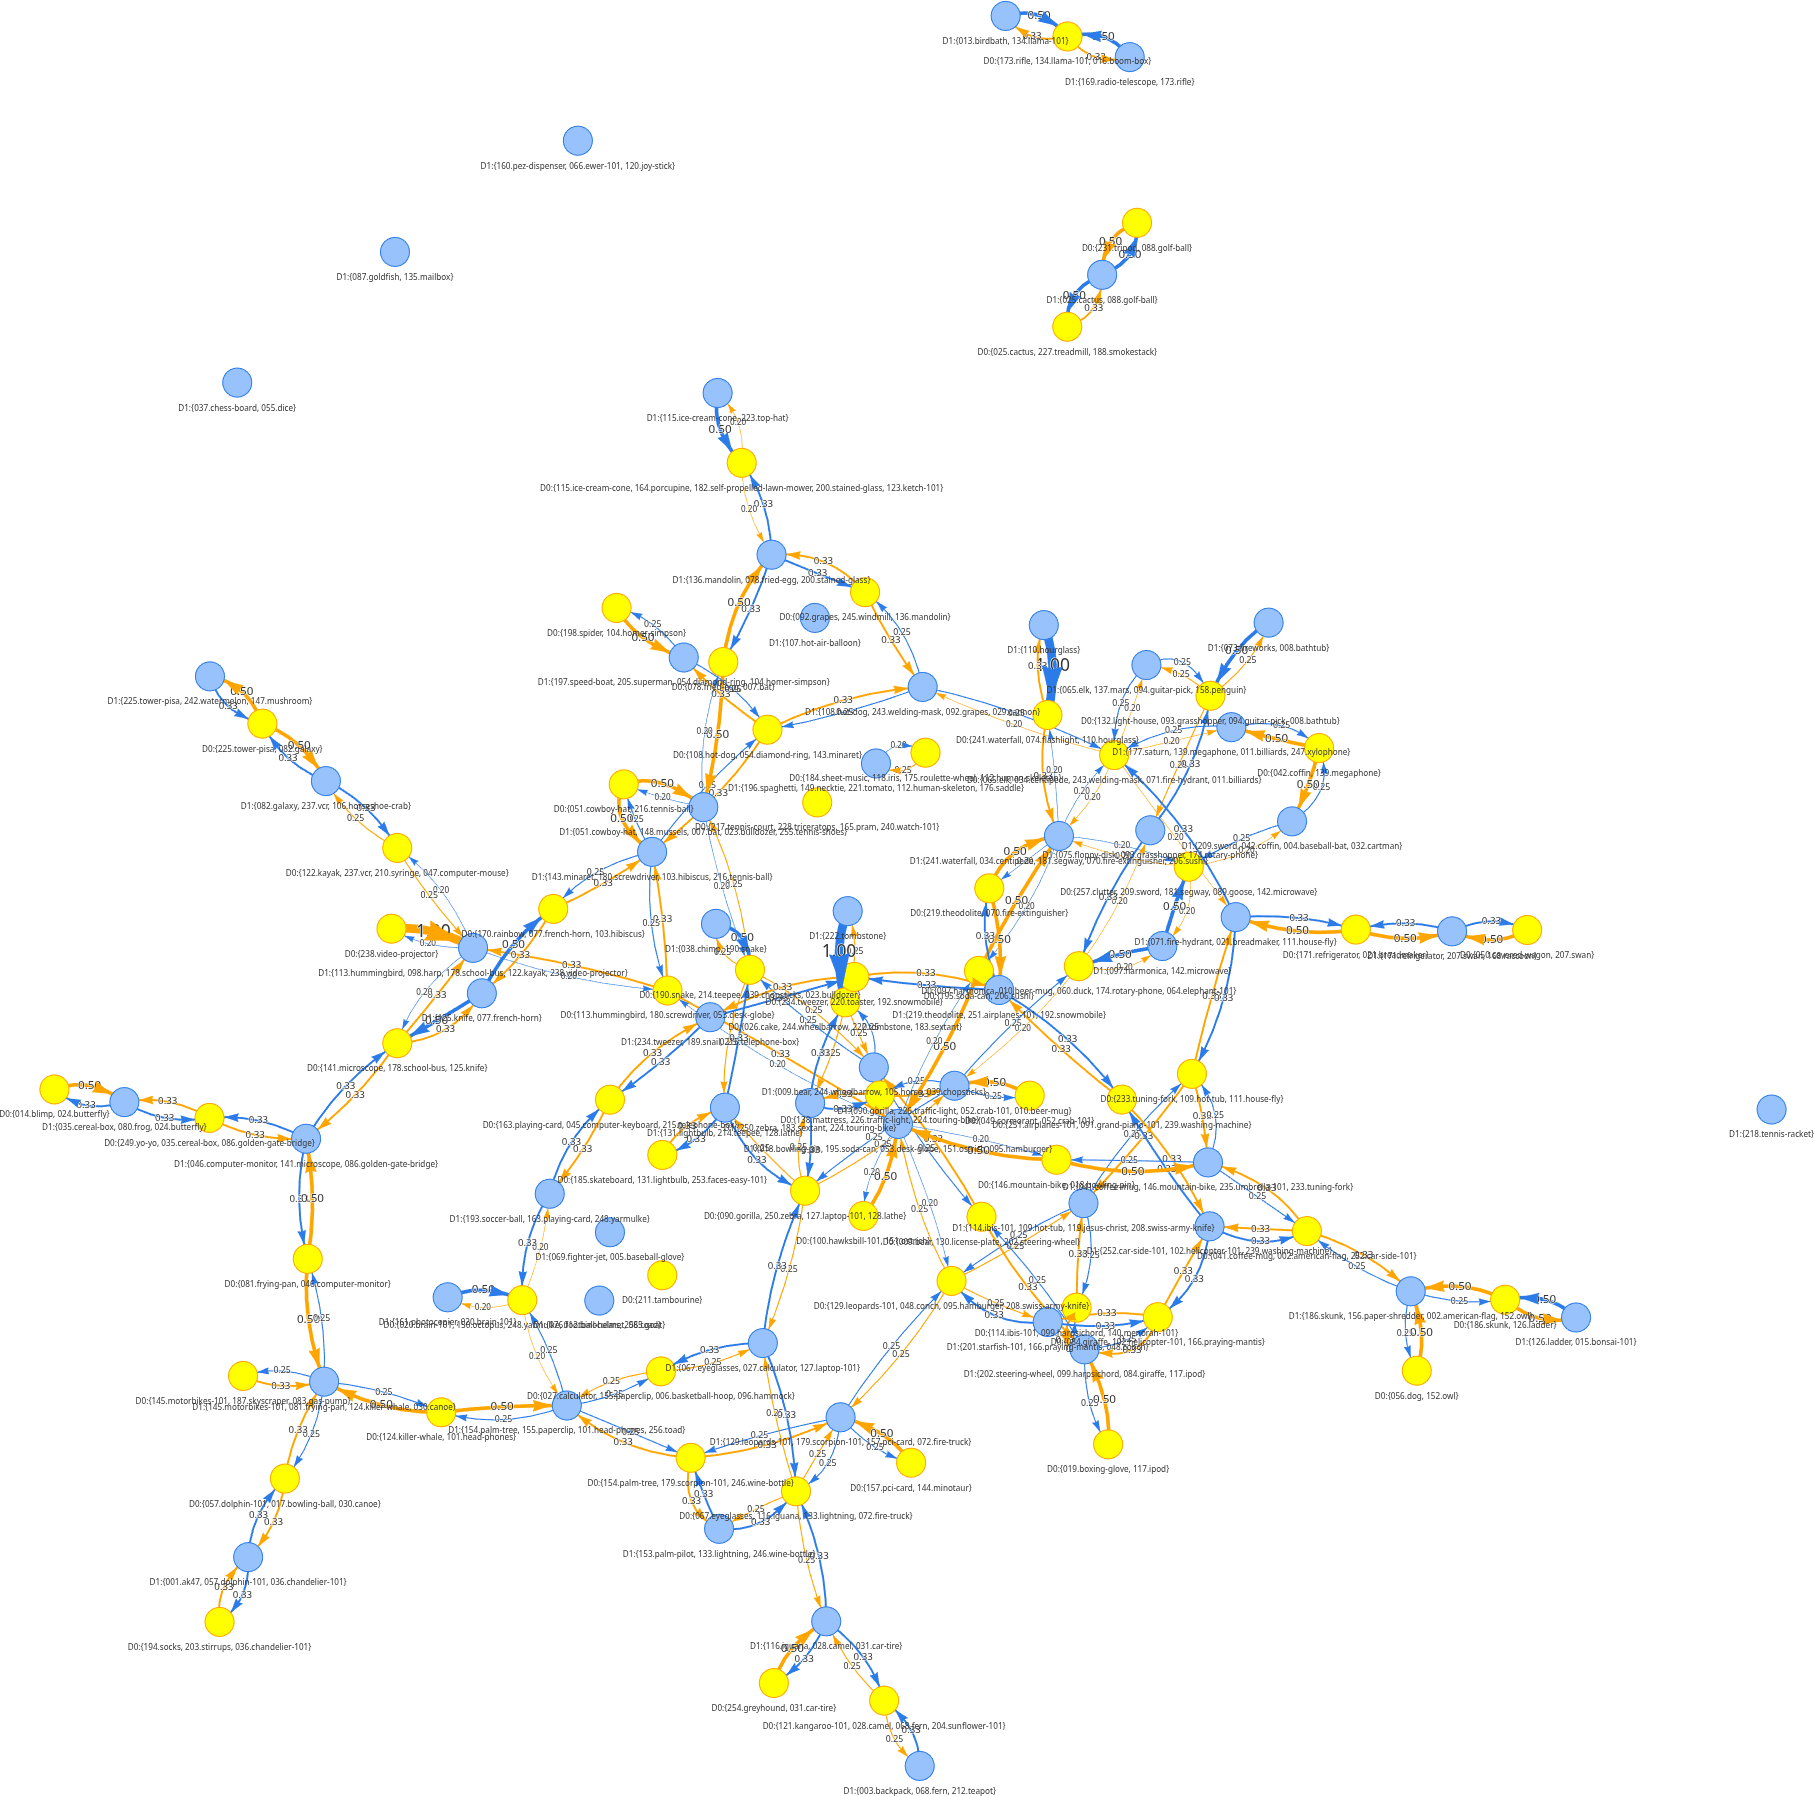
\includegraphics[width=0.6\textwidth]{figures/caltech256_2domain.png}
      \caption{Caltech-256 2-domain synthetic dataset variant.
      The number of concepts is sampled from a truncated normal distribution
      with a $\mu_{\text{concepts}}=180$ and $\sigma^2_{\text{concepts}}=10$,
      while the number of classes per concept is sampled from a truncated normal distribution
      with a $\mu_{\text{classes}}=3$ and $\sigma^2_{\text{classes}}=1$.}
      \label{fig:caltech256_2domain}
\end{figure}

\begin{figure}[ht]
      \centering
      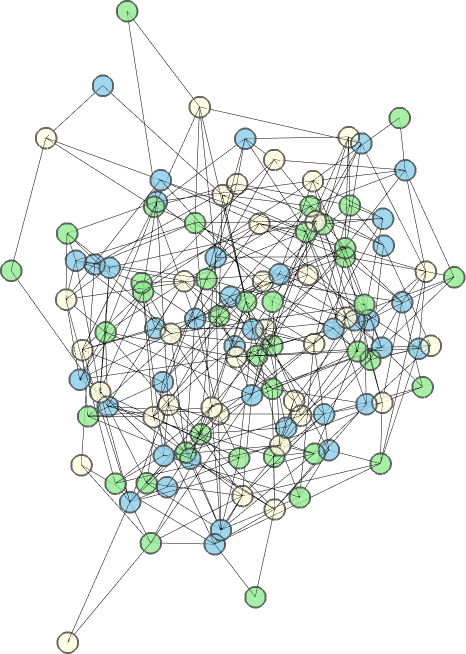
\includegraphics[width=0.6\textwidth]{figures/caltech256_3domain.png}
      \caption{Caltech-256 3-domain synthetic dataset variant rendered in a 3D scatter plot.
      The number of concepts is sampled from a truncated normal distribution
      with a $\mu_{\text{concepts}}=180$ and $\sigma^2_{\text{concepts}}=10$,
      while the number of classes per concept is sampled from a truncated normal distribution
      with a $\mu_{\text{classes}}=5$ and $\sigma^2_{\text{classes}}=1$.}
      \label{fig:caltech256_3domain}
\end{figure}

\begin{figure}[ht]
      \centering
      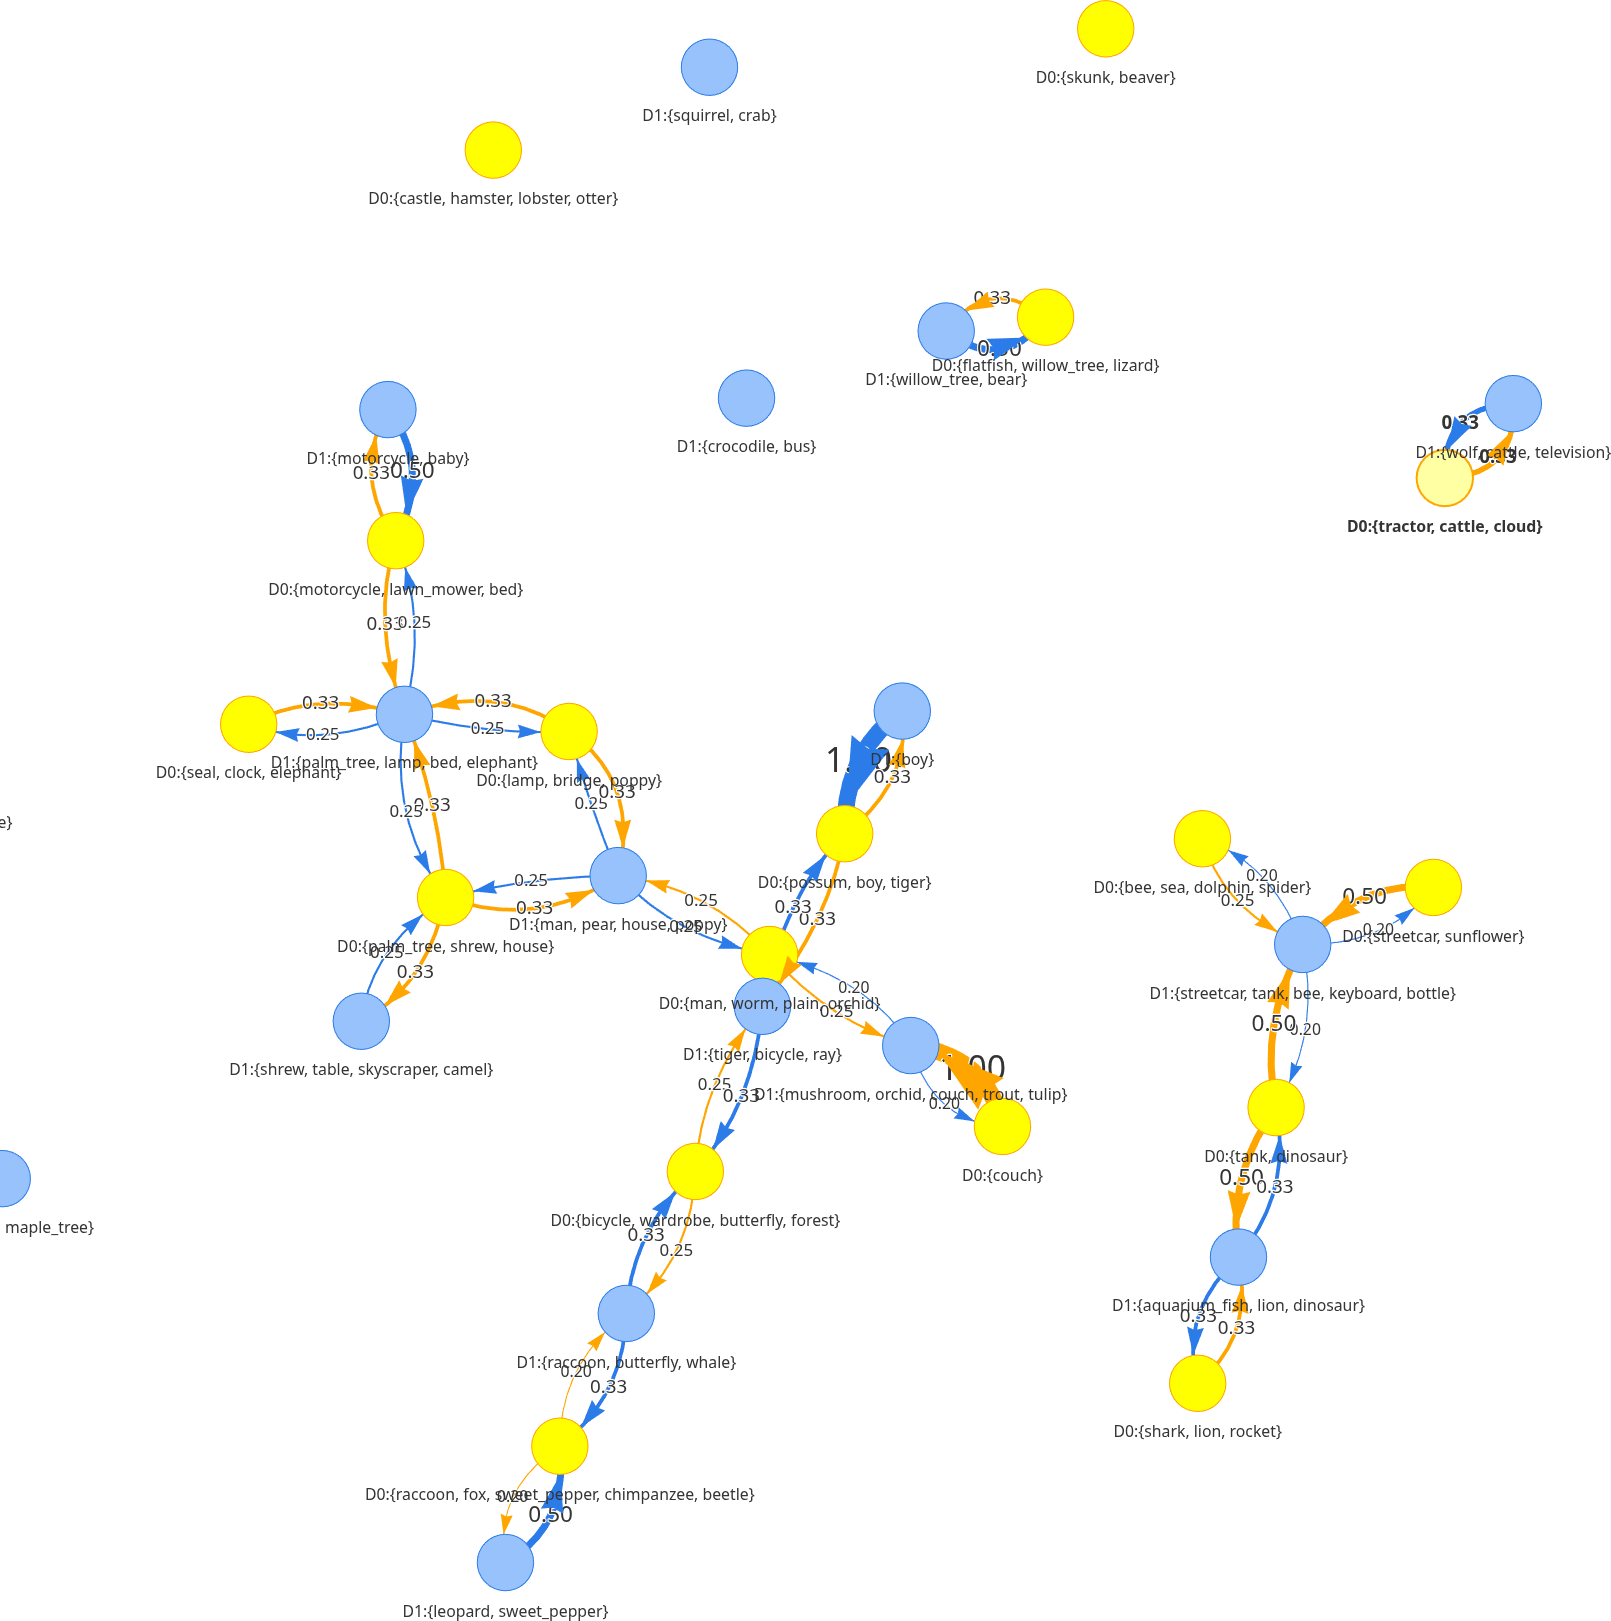
\includegraphics[width=0.6\textwidth]{figures/cifar100_2domain.png}
      \caption{CIFAR-100 2-domain synthetic dataset variant.
      The number of concepts is sampled from a truncated normal distribution
      with a $\mu_{\text{concepts}}=50$ and $\sigma^2_{\text{concepts}}=5$,
      while the number of classes per concept is sampled from a truncated normal distribution
      with a $\mu_{\text{classes}}=3$ and $\sigma^2_{\text{classes}}=1$.}
      \label{fig:cifar100_2domain}
\end{figure}

\subsubsection{Model Accuracy}

Let us now take a look at the accuracy of our models trained on the synthetic dataset variants.
We use checkpoints to save the model after each epoch and pick the model checkpoint with the lowest validation loss
for our final evaluation.

We can see our final training runs in Figures~\ref{fig:caltech256_2domain_accuracy}, \ref{fig:caltech256_3domain_accuracy}, and \ref{fig:cifar100_2domain_accuracy}.
It can be observed that our overfitting mitigation techniques have worked sufficiently well,
as our training and validation accuracy curves do not diverge significantly.
We present the final model accuracies on the test sets in Table~\ref{tab:evaluation_results}.
Multiple things can be observed:
\begin{itemize}
      \item All the models achieve an accuracy of around 0.8 on the test set,
            which is an average performance for these datasets.
            Our focus is not on achieving state-of-the-art performance,
            but rather on creating models suitable for our cross-domain prediction task.
            It should be noted that a lower model accuracy will lead to worse performance
            in our relationship selection methods, but since we will compare the methods against each other
            using the same models, this should not be a problem.
      \item The CIFAR-100 variants have a slightly lower accuracy than the Caltech-256 variants,
            which is expected since the CIFAR-100 dataset has closely related classes
            categorised into superclasses, which make it harder for a model to distinguish between them.
      \item The number of concepts (i.e. classes) in the original dataset that get merged
            into a new class in the synthetic dataset variants does not seem to have a significant impact
            on the model accuracy: The Caltech-256 2-domain variant has a $\mu_{\text{classes}}=3$,
            while the Caltech-256 3-domain variant has a $\mu_{\text{classes}}=5$,
            but the deviation in accuracy is negligible ($\leq 0.01$).
\end{itemize}

\begin{figure}[ht]
      \centering
      \scalebox{0.6}{%% Creator: Matplotlib, PGF backend
%%
%% To include the figure in your LaTeX document, write
%%   \input{<filename>.pgf}
%%
%% Make sure the required packages are loaded in your preamble
%%   \usepackage{pgf}
%%
%% Also ensure that all the required font packages are loaded; for instance,
%% the lmodern package is sometimes necessary when using math font.
%%   \usepackage{lmodern}
%%
%% Figures using additional raster images can only be included by \input if
%% they are in the same directory as the main LaTeX file. For loading figures
%% from other directories you can use the `import` package
%%   \usepackage{import}
%%
%% and then include the figures with
%%   \import{<path to file>}{<filename>.pgf}
%%
%% Matplotlib used the following preamble
%%   \def\mathdefault#1{#1}
%%   \everymath=\expandafter{\the\everymath\displaystyle}
%%   \IfFileExists{scrextend.sty}{
%%     \usepackage[fontsize=11.000000pt]{scrextend}
%%   }{
%%     \renewcommand{\normalsize}{\fontsize{11.000000}{13.200000}\selectfont}
%%     \normalsize
%%   }
%%   
%%   \ifdefined\pdftexversion\else  % non-pdftex case.
%%     \usepackage{fontspec}
%%     \setmainfont{DejaVuSerif.ttf}[Path=\detokenize{/home/sentinel/.conda/envs/master-thesis/lib/python3.13/site-packages/matplotlib/mpl-data/fonts/ttf/}]
%%     \setsansfont{DejaVuSans.ttf}[Path=\detokenize{/home/sentinel/.conda/envs/master-thesis/lib/python3.13/site-packages/matplotlib/mpl-data/fonts/ttf/}]
%%     \setmonofont{DejaVuSansMono.ttf}[Path=\detokenize{/home/sentinel/.conda/envs/master-thesis/lib/python3.13/site-packages/matplotlib/mpl-data/fonts/ttf/}]
%%   \fi
%%   \makeatletter\@ifpackageloaded{underscore}{}{\usepackage[strings]{underscore}}\makeatother
%%
\begingroup%
\makeatletter%
\begin{pgfpicture}%
\pgfpathrectangle{\pgfpointorigin}{\pgfqpoint{5.376214in}{3.951110in}}%
\pgfusepath{use as bounding box, clip}%
\begin{pgfscope}%
\pgfsetbuttcap%
\pgfsetmiterjoin%
\definecolor{currentfill}{rgb}{1.000000,1.000000,1.000000}%
\pgfsetfillcolor{currentfill}%
\pgfsetlinewidth{0.000000pt}%
\definecolor{currentstroke}{rgb}{1.000000,1.000000,1.000000}%
\pgfsetstrokecolor{currentstroke}%
\pgfsetdash{}{0pt}%
\pgfpathmoveto{\pgfqpoint{0.000000in}{0.000000in}}%
\pgfpathlineto{\pgfqpoint{5.376214in}{0.000000in}}%
\pgfpathlineto{\pgfqpoint{5.376214in}{3.951110in}}%
\pgfpathlineto{\pgfqpoint{0.000000in}{3.951110in}}%
\pgfpathlineto{\pgfqpoint{0.000000in}{0.000000in}}%
\pgfpathclose%
\pgfusepath{fill}%
\end{pgfscope}%
\begin{pgfscope}%
\pgfsetbuttcap%
\pgfsetmiterjoin%
\definecolor{currentfill}{rgb}{1.000000,1.000000,1.000000}%
\pgfsetfillcolor{currentfill}%
\pgfsetlinewidth{0.000000pt}%
\definecolor{currentstroke}{rgb}{0.000000,0.000000,0.000000}%
\pgfsetstrokecolor{currentstroke}%
\pgfsetstrokeopacity{0.000000}%
\pgfsetdash{}{0pt}%
\pgfpathmoveto{\pgfqpoint{0.594961in}{0.548486in}}%
\pgfpathlineto{\pgfqpoint{5.244961in}{0.548486in}}%
\pgfpathlineto{\pgfqpoint{5.244961in}{3.628486in}}%
\pgfpathlineto{\pgfqpoint{0.594961in}{3.628486in}}%
\pgfpathlineto{\pgfqpoint{0.594961in}{0.548486in}}%
\pgfpathclose%
\pgfusepath{fill}%
\end{pgfscope}%
\begin{pgfscope}%
\pgfsetbuttcap%
\pgfsetroundjoin%
\definecolor{currentfill}{rgb}{0.000000,0.000000,0.000000}%
\pgfsetfillcolor{currentfill}%
\pgfsetlinewidth{0.803000pt}%
\definecolor{currentstroke}{rgb}{0.000000,0.000000,0.000000}%
\pgfsetstrokecolor{currentstroke}%
\pgfsetdash{}{0pt}%
\pgfsys@defobject{currentmarker}{\pgfqpoint{0.000000in}{-0.048611in}}{\pgfqpoint{0.000000in}{0.000000in}}{%
\pgfpathmoveto{\pgfqpoint{0.000000in}{0.000000in}}%
\pgfpathlineto{\pgfqpoint{0.000000in}{-0.048611in}}%
\pgfusepath{stroke,fill}%
}%
\begin{pgfscope}%
\pgfsys@transformshift{0.768457in}{0.548486in}%
\pgfsys@useobject{currentmarker}{}%
\end{pgfscope}%
\end{pgfscope}%
\begin{pgfscope}%
\definecolor{textcolor}{rgb}{0.000000,0.000000,0.000000}%
\pgfsetstrokecolor{textcolor}%
\pgfsetfillcolor{textcolor}%
\pgftext[x=0.768457in,y=0.451264in,,top]{\color{textcolor}{\fontsize{11.000000}{13.200000}\selectfont\catcode`\^=\active\def^{\ifmmode\sp\else\^{}\fi}\catcode`\%=\active\def%{\%}$\mathdefault{0}$}}%
\end{pgfscope}%
\begin{pgfscope}%
\pgfsetbuttcap%
\pgfsetroundjoin%
\definecolor{currentfill}{rgb}{0.000000,0.000000,0.000000}%
\pgfsetfillcolor{currentfill}%
\pgfsetlinewidth{0.803000pt}%
\definecolor{currentstroke}{rgb}{0.000000,0.000000,0.000000}%
\pgfsetstrokecolor{currentstroke}%
\pgfsetdash{}{0pt}%
\pgfsys@defobject{currentmarker}{\pgfqpoint{0.000000in}{-0.048611in}}{\pgfqpoint{0.000000in}{0.000000in}}{%
\pgfpathmoveto{\pgfqpoint{0.000000in}{0.000000in}}%
\pgfpathlineto{\pgfqpoint{0.000000in}{-0.048611in}}%
\pgfusepath{stroke,fill}%
}%
\begin{pgfscope}%
\pgfsys@transformshift{1.541267in}{0.548486in}%
\pgfsys@useobject{currentmarker}{}%
\end{pgfscope}%
\end{pgfscope}%
\begin{pgfscope}%
\definecolor{textcolor}{rgb}{0.000000,0.000000,0.000000}%
\pgfsetstrokecolor{textcolor}%
\pgfsetfillcolor{textcolor}%
\pgftext[x=1.541267in,y=0.451264in,,top]{\color{textcolor}{\fontsize{11.000000}{13.200000}\selectfont\catcode`\^=\active\def^{\ifmmode\sp\else\^{}\fi}\catcode`\%=\active\def%{\%}$\mathdefault{1000}$}}%
\end{pgfscope}%
\begin{pgfscope}%
\pgfsetbuttcap%
\pgfsetroundjoin%
\definecolor{currentfill}{rgb}{0.000000,0.000000,0.000000}%
\pgfsetfillcolor{currentfill}%
\pgfsetlinewidth{0.803000pt}%
\definecolor{currentstroke}{rgb}{0.000000,0.000000,0.000000}%
\pgfsetstrokecolor{currentstroke}%
\pgfsetdash{}{0pt}%
\pgfsys@defobject{currentmarker}{\pgfqpoint{0.000000in}{-0.048611in}}{\pgfqpoint{0.000000in}{0.000000in}}{%
\pgfpathmoveto{\pgfqpoint{0.000000in}{0.000000in}}%
\pgfpathlineto{\pgfqpoint{0.000000in}{-0.048611in}}%
\pgfusepath{stroke,fill}%
}%
\begin{pgfscope}%
\pgfsys@transformshift{2.314078in}{0.548486in}%
\pgfsys@useobject{currentmarker}{}%
\end{pgfscope}%
\end{pgfscope}%
\begin{pgfscope}%
\definecolor{textcolor}{rgb}{0.000000,0.000000,0.000000}%
\pgfsetstrokecolor{textcolor}%
\pgfsetfillcolor{textcolor}%
\pgftext[x=2.314078in,y=0.451264in,,top]{\color{textcolor}{\fontsize{11.000000}{13.200000}\selectfont\catcode`\^=\active\def^{\ifmmode\sp\else\^{}\fi}\catcode`\%=\active\def%{\%}$\mathdefault{2000}$}}%
\end{pgfscope}%
\begin{pgfscope}%
\pgfsetbuttcap%
\pgfsetroundjoin%
\definecolor{currentfill}{rgb}{0.000000,0.000000,0.000000}%
\pgfsetfillcolor{currentfill}%
\pgfsetlinewidth{0.803000pt}%
\definecolor{currentstroke}{rgb}{0.000000,0.000000,0.000000}%
\pgfsetstrokecolor{currentstroke}%
\pgfsetdash{}{0pt}%
\pgfsys@defobject{currentmarker}{\pgfqpoint{0.000000in}{-0.048611in}}{\pgfqpoint{0.000000in}{0.000000in}}{%
\pgfpathmoveto{\pgfqpoint{0.000000in}{0.000000in}}%
\pgfpathlineto{\pgfqpoint{0.000000in}{-0.048611in}}%
\pgfusepath{stroke,fill}%
}%
\begin{pgfscope}%
\pgfsys@transformshift{3.086888in}{0.548486in}%
\pgfsys@useobject{currentmarker}{}%
\end{pgfscope}%
\end{pgfscope}%
\begin{pgfscope}%
\definecolor{textcolor}{rgb}{0.000000,0.000000,0.000000}%
\pgfsetstrokecolor{textcolor}%
\pgfsetfillcolor{textcolor}%
\pgftext[x=3.086888in,y=0.451264in,,top]{\color{textcolor}{\fontsize{11.000000}{13.200000}\selectfont\catcode`\^=\active\def^{\ifmmode\sp\else\^{}\fi}\catcode`\%=\active\def%{\%}$\mathdefault{3000}$}}%
\end{pgfscope}%
\begin{pgfscope}%
\pgfsetbuttcap%
\pgfsetroundjoin%
\definecolor{currentfill}{rgb}{0.000000,0.000000,0.000000}%
\pgfsetfillcolor{currentfill}%
\pgfsetlinewidth{0.803000pt}%
\definecolor{currentstroke}{rgb}{0.000000,0.000000,0.000000}%
\pgfsetstrokecolor{currentstroke}%
\pgfsetdash{}{0pt}%
\pgfsys@defobject{currentmarker}{\pgfqpoint{0.000000in}{-0.048611in}}{\pgfqpoint{0.000000in}{0.000000in}}{%
\pgfpathmoveto{\pgfqpoint{0.000000in}{0.000000in}}%
\pgfpathlineto{\pgfqpoint{0.000000in}{-0.048611in}}%
\pgfusepath{stroke,fill}%
}%
\begin{pgfscope}%
\pgfsys@transformshift{3.859698in}{0.548486in}%
\pgfsys@useobject{currentmarker}{}%
\end{pgfscope}%
\end{pgfscope}%
\begin{pgfscope}%
\definecolor{textcolor}{rgb}{0.000000,0.000000,0.000000}%
\pgfsetstrokecolor{textcolor}%
\pgfsetfillcolor{textcolor}%
\pgftext[x=3.859698in,y=0.451264in,,top]{\color{textcolor}{\fontsize{11.000000}{13.200000}\selectfont\catcode`\^=\active\def^{\ifmmode\sp\else\^{}\fi}\catcode`\%=\active\def%{\%}$\mathdefault{4000}$}}%
\end{pgfscope}%
\begin{pgfscope}%
\pgfsetbuttcap%
\pgfsetroundjoin%
\definecolor{currentfill}{rgb}{0.000000,0.000000,0.000000}%
\pgfsetfillcolor{currentfill}%
\pgfsetlinewidth{0.803000pt}%
\definecolor{currentstroke}{rgb}{0.000000,0.000000,0.000000}%
\pgfsetstrokecolor{currentstroke}%
\pgfsetdash{}{0pt}%
\pgfsys@defobject{currentmarker}{\pgfqpoint{0.000000in}{-0.048611in}}{\pgfqpoint{0.000000in}{0.000000in}}{%
\pgfpathmoveto{\pgfqpoint{0.000000in}{0.000000in}}%
\pgfpathlineto{\pgfqpoint{0.000000in}{-0.048611in}}%
\pgfusepath{stroke,fill}%
}%
\begin{pgfscope}%
\pgfsys@transformshift{4.632509in}{0.548486in}%
\pgfsys@useobject{currentmarker}{}%
\end{pgfscope}%
\end{pgfscope}%
\begin{pgfscope}%
\definecolor{textcolor}{rgb}{0.000000,0.000000,0.000000}%
\pgfsetstrokecolor{textcolor}%
\pgfsetfillcolor{textcolor}%
\pgftext[x=4.632509in,y=0.451264in,,top]{\color{textcolor}{\fontsize{11.000000}{13.200000}\selectfont\catcode`\^=\active\def^{\ifmmode\sp\else\^{}\fi}\catcode`\%=\active\def%{\%}$\mathdefault{5000}$}}%
\end{pgfscope}%
\begin{pgfscope}%
\definecolor{textcolor}{rgb}{0.000000,0.000000,0.000000}%
\pgfsetstrokecolor{textcolor}%
\pgfsetfillcolor{textcolor}%
\pgftext[x=2.919961in,y=0.247854in,,top]{\color{textcolor}{\fontsize{11.000000}{13.200000}\selectfont\catcode`\^=\active\def^{\ifmmode\sp\else\^{}\fi}\catcode`\%=\active\def%{\%}Steps}}%
\end{pgfscope}%
\begin{pgfscope}%
\pgfsetbuttcap%
\pgfsetroundjoin%
\definecolor{currentfill}{rgb}{0.000000,0.000000,0.000000}%
\pgfsetfillcolor{currentfill}%
\pgfsetlinewidth{0.803000pt}%
\definecolor{currentstroke}{rgb}{0.000000,0.000000,0.000000}%
\pgfsetstrokecolor{currentstroke}%
\pgfsetdash{}{0pt}%
\pgfsys@defobject{currentmarker}{\pgfqpoint{-0.048611in}{0.000000in}}{\pgfqpoint{-0.000000in}{0.000000in}}{%
\pgfpathmoveto{\pgfqpoint{-0.000000in}{0.000000in}}%
\pgfpathlineto{\pgfqpoint{-0.048611in}{0.000000in}}%
\pgfusepath{stroke,fill}%
}%
\begin{pgfscope}%
\pgfsys@transformshift{0.594961in}{0.881941in}%
\pgfsys@useobject{currentmarker}{}%
\end{pgfscope}%
\end{pgfscope}%
\begin{pgfscope}%
\definecolor{textcolor}{rgb}{0.000000,0.000000,0.000000}%
\pgfsetstrokecolor{textcolor}%
\pgfsetfillcolor{textcolor}%
\pgftext[x=0.303410in, y=0.823903in, left, base]{\color{textcolor}{\fontsize{11.000000}{13.200000}\selectfont\catcode`\^=\active\def^{\ifmmode\sp\else\^{}\fi}\catcode`\%=\active\def%{\%}$\mathdefault{0.2}$}}%
\end{pgfscope}%
\begin{pgfscope}%
\pgfsetbuttcap%
\pgfsetroundjoin%
\definecolor{currentfill}{rgb}{0.000000,0.000000,0.000000}%
\pgfsetfillcolor{currentfill}%
\pgfsetlinewidth{0.803000pt}%
\definecolor{currentstroke}{rgb}{0.000000,0.000000,0.000000}%
\pgfsetstrokecolor{currentstroke}%
\pgfsetdash{}{0pt}%
\pgfsys@defobject{currentmarker}{\pgfqpoint{-0.048611in}{0.000000in}}{\pgfqpoint{-0.000000in}{0.000000in}}{%
\pgfpathmoveto{\pgfqpoint{-0.000000in}{0.000000in}}%
\pgfpathlineto{\pgfqpoint{-0.048611in}{0.000000in}}%
\pgfusepath{stroke,fill}%
}%
\begin{pgfscope}%
\pgfsys@transformshift{0.594961in}{1.533577in}%
\pgfsys@useobject{currentmarker}{}%
\end{pgfscope}%
\end{pgfscope}%
\begin{pgfscope}%
\definecolor{textcolor}{rgb}{0.000000,0.000000,0.000000}%
\pgfsetstrokecolor{textcolor}%
\pgfsetfillcolor{textcolor}%
\pgftext[x=0.303410in, y=1.475540in, left, base]{\color{textcolor}{\fontsize{11.000000}{13.200000}\selectfont\catcode`\^=\active\def^{\ifmmode\sp\else\^{}\fi}\catcode`\%=\active\def%{\%}$\mathdefault{0.4}$}}%
\end{pgfscope}%
\begin{pgfscope}%
\pgfsetbuttcap%
\pgfsetroundjoin%
\definecolor{currentfill}{rgb}{0.000000,0.000000,0.000000}%
\pgfsetfillcolor{currentfill}%
\pgfsetlinewidth{0.803000pt}%
\definecolor{currentstroke}{rgb}{0.000000,0.000000,0.000000}%
\pgfsetstrokecolor{currentstroke}%
\pgfsetdash{}{0pt}%
\pgfsys@defobject{currentmarker}{\pgfqpoint{-0.048611in}{0.000000in}}{\pgfqpoint{-0.000000in}{0.000000in}}{%
\pgfpathmoveto{\pgfqpoint{-0.000000in}{0.000000in}}%
\pgfpathlineto{\pgfqpoint{-0.048611in}{0.000000in}}%
\pgfusepath{stroke,fill}%
}%
\begin{pgfscope}%
\pgfsys@transformshift{0.594961in}{2.185214in}%
\pgfsys@useobject{currentmarker}{}%
\end{pgfscope}%
\end{pgfscope}%
\begin{pgfscope}%
\definecolor{textcolor}{rgb}{0.000000,0.000000,0.000000}%
\pgfsetstrokecolor{textcolor}%
\pgfsetfillcolor{textcolor}%
\pgftext[x=0.303410in, y=2.127176in, left, base]{\color{textcolor}{\fontsize{11.000000}{13.200000}\selectfont\catcode`\^=\active\def^{\ifmmode\sp\else\^{}\fi}\catcode`\%=\active\def%{\%}$\mathdefault{0.6}$}}%
\end{pgfscope}%
\begin{pgfscope}%
\pgfsetbuttcap%
\pgfsetroundjoin%
\definecolor{currentfill}{rgb}{0.000000,0.000000,0.000000}%
\pgfsetfillcolor{currentfill}%
\pgfsetlinewidth{0.803000pt}%
\definecolor{currentstroke}{rgb}{0.000000,0.000000,0.000000}%
\pgfsetstrokecolor{currentstroke}%
\pgfsetdash{}{0pt}%
\pgfsys@defobject{currentmarker}{\pgfqpoint{-0.048611in}{0.000000in}}{\pgfqpoint{-0.000000in}{0.000000in}}{%
\pgfpathmoveto{\pgfqpoint{-0.000000in}{0.000000in}}%
\pgfpathlineto{\pgfqpoint{-0.048611in}{0.000000in}}%
\pgfusepath{stroke,fill}%
}%
\begin{pgfscope}%
\pgfsys@transformshift{0.594961in}{2.836850in}%
\pgfsys@useobject{currentmarker}{}%
\end{pgfscope}%
\end{pgfscope}%
\begin{pgfscope}%
\definecolor{textcolor}{rgb}{0.000000,0.000000,0.000000}%
\pgfsetstrokecolor{textcolor}%
\pgfsetfillcolor{textcolor}%
\pgftext[x=0.303410in, y=2.778812in, left, base]{\color{textcolor}{\fontsize{11.000000}{13.200000}\selectfont\catcode`\^=\active\def^{\ifmmode\sp\else\^{}\fi}\catcode`\%=\active\def%{\%}$\mathdefault{0.8}$}}%
\end{pgfscope}%
\begin{pgfscope}%
\pgfsetbuttcap%
\pgfsetroundjoin%
\definecolor{currentfill}{rgb}{0.000000,0.000000,0.000000}%
\pgfsetfillcolor{currentfill}%
\pgfsetlinewidth{0.803000pt}%
\definecolor{currentstroke}{rgb}{0.000000,0.000000,0.000000}%
\pgfsetstrokecolor{currentstroke}%
\pgfsetdash{}{0pt}%
\pgfsys@defobject{currentmarker}{\pgfqpoint{-0.048611in}{0.000000in}}{\pgfqpoint{-0.000000in}{0.000000in}}{%
\pgfpathmoveto{\pgfqpoint{-0.000000in}{0.000000in}}%
\pgfpathlineto{\pgfqpoint{-0.048611in}{0.000000in}}%
\pgfusepath{stroke,fill}%
}%
\begin{pgfscope}%
\pgfsys@transformshift{0.594961in}{3.488486in}%
\pgfsys@useobject{currentmarker}{}%
\end{pgfscope}%
\end{pgfscope}%
\begin{pgfscope}%
\definecolor{textcolor}{rgb}{0.000000,0.000000,0.000000}%
\pgfsetstrokecolor{textcolor}%
\pgfsetfillcolor{textcolor}%
\pgftext[x=0.303410in, y=3.430449in, left, base]{\color{textcolor}{\fontsize{11.000000}{13.200000}\selectfont\catcode`\^=\active\def^{\ifmmode\sp\else\^{}\fi}\catcode`\%=\active\def%{\%}$\mathdefault{1.0}$}}%
\end{pgfscope}%
\begin{pgfscope}%
\definecolor{textcolor}{rgb}{0.000000,0.000000,0.000000}%
\pgfsetstrokecolor{textcolor}%
\pgfsetfillcolor{textcolor}%
\pgftext[x=0.247854in,y=2.088486in,,bottom,rotate=90.000000]{\color{textcolor}{\fontsize{11.000000}{13.200000}\selectfont\catcode`\^=\active\def^{\ifmmode\sp\else\^{}\fi}\catcode`\%=\active\def%{\%}Accuracy}}%
\end{pgfscope}%
\begin{pgfscope}%
\pgfpathrectangle{\pgfqpoint{0.594961in}{0.548486in}}{\pgfqpoint{4.650000in}{3.080000in}}%
\pgfusepath{clip}%
\pgfsetrectcap%
\pgfsetroundjoin%
\pgfsetlinewidth{1.505625pt}%
\definecolor{currentstroke}{rgb}{0.121569,0.466667,0.705882}%
\pgfsetstrokecolor{currentstroke}%
\pgfsetdash{}{0pt}%
\pgfpathmoveto{\pgfqpoint{0.806325in}{0.688486in}}%
\pgfpathlineto{\pgfqpoint{0.844965in}{0.739395in}}%
\pgfpathlineto{\pgfqpoint{0.883606in}{0.892123in}}%
\pgfpathlineto{\pgfqpoint{0.922246in}{1.553941in}}%
\pgfpathlineto{\pgfqpoint{0.960887in}{1.808486in}}%
\pgfpathlineto{\pgfqpoint{0.999527in}{1.910305in}}%
\pgfpathlineto{\pgfqpoint{1.038168in}{2.368486in}}%
\pgfpathlineto{\pgfqpoint{1.076808in}{2.368486in}}%
\pgfpathlineto{\pgfqpoint{1.115449in}{2.623032in}}%
\pgfpathlineto{\pgfqpoint{1.154089in}{2.775759in}}%
\pgfpathlineto{\pgfqpoint{1.192730in}{2.979395in}}%
\pgfpathlineto{\pgfqpoint{1.231370in}{2.826668in}}%
\pgfpathlineto{\pgfqpoint{1.270011in}{2.928486in}}%
\pgfpathlineto{\pgfqpoint{1.308651in}{2.572123in}}%
\pgfpathlineto{\pgfqpoint{1.347292in}{3.183032in}}%
\pgfpathlineto{\pgfqpoint{1.385932in}{2.928486in}}%
\pgfpathlineto{\pgfqpoint{1.424573in}{3.132123in}}%
\pgfpathlineto{\pgfqpoint{1.463213in}{3.030305in}}%
\pgfpathlineto{\pgfqpoint{1.501854in}{3.233941in}}%
\pgfpathlineto{\pgfqpoint{1.540494in}{3.233941in}}%
\pgfpathlineto{\pgfqpoint{1.579135in}{2.775759in}}%
\pgfpathlineto{\pgfqpoint{1.617775in}{2.877577in}}%
\pgfpathlineto{\pgfqpoint{1.656416in}{2.928486in}}%
\pgfpathlineto{\pgfqpoint{1.695057in}{3.030305in}}%
\pgfpathlineto{\pgfqpoint{1.733697in}{2.979395in}}%
\pgfpathlineto{\pgfqpoint{1.772338in}{3.081214in}}%
\pgfpathlineto{\pgfqpoint{1.810978in}{3.386668in}}%
\pgfpathlineto{\pgfqpoint{1.849619in}{3.284850in}}%
\pgfpathlineto{\pgfqpoint{1.888259in}{3.132123in}}%
\pgfpathlineto{\pgfqpoint{1.926900in}{3.183032in}}%
\pgfpathlineto{\pgfqpoint{1.965540in}{3.132123in}}%
\pgfpathlineto{\pgfqpoint{2.004181in}{3.233941in}}%
\pgfpathlineto{\pgfqpoint{2.042821in}{3.183032in}}%
\pgfpathlineto{\pgfqpoint{2.081462in}{3.335759in}}%
\pgfpathlineto{\pgfqpoint{2.120102in}{3.284850in}}%
\pgfpathlineto{\pgfqpoint{2.158743in}{3.284850in}}%
\pgfpathlineto{\pgfqpoint{2.197383in}{3.233941in}}%
\pgfpathlineto{\pgfqpoint{2.236024in}{3.335759in}}%
\pgfpathlineto{\pgfqpoint{2.274664in}{3.386668in}}%
\pgfpathlineto{\pgfqpoint{2.313305in}{3.284850in}}%
\pgfpathlineto{\pgfqpoint{2.351945in}{3.284850in}}%
\pgfpathlineto{\pgfqpoint{2.390586in}{3.132123in}}%
\pgfpathlineto{\pgfqpoint{2.429226in}{3.335759in}}%
\pgfpathlineto{\pgfqpoint{2.467867in}{3.132123in}}%
\pgfpathlineto{\pgfqpoint{2.506507in}{3.335759in}}%
\pgfpathlineto{\pgfqpoint{2.545148in}{2.979395in}}%
\pgfpathlineto{\pgfqpoint{2.583788in}{3.233941in}}%
\pgfpathlineto{\pgfqpoint{2.622429in}{3.233941in}}%
\pgfpathlineto{\pgfqpoint{2.661069in}{3.335759in}}%
\pgfpathlineto{\pgfqpoint{2.699710in}{3.386668in}}%
\pgfpathlineto{\pgfqpoint{2.738351in}{3.284850in}}%
\pgfpathlineto{\pgfqpoint{2.776991in}{3.233941in}}%
\pgfpathlineto{\pgfqpoint{2.815632in}{3.233941in}}%
\pgfpathlineto{\pgfqpoint{2.854272in}{3.437577in}}%
\pgfpathlineto{\pgfqpoint{2.892913in}{3.233941in}}%
\pgfpathlineto{\pgfqpoint{2.931553in}{3.386668in}}%
\pgfpathlineto{\pgfqpoint{2.970194in}{3.335759in}}%
\pgfpathlineto{\pgfqpoint{3.008834in}{3.284850in}}%
\pgfpathlineto{\pgfqpoint{3.047475in}{3.488486in}}%
\pgfpathlineto{\pgfqpoint{3.086115in}{3.437577in}}%
\pgfpathlineto{\pgfqpoint{3.124756in}{3.386668in}}%
\pgfpathlineto{\pgfqpoint{3.163396in}{3.437577in}}%
\pgfpathlineto{\pgfqpoint{3.202037in}{3.335759in}}%
\pgfpathlineto{\pgfqpoint{3.240677in}{3.233941in}}%
\pgfpathlineto{\pgfqpoint{3.279318in}{3.284850in}}%
\pgfpathlineto{\pgfqpoint{3.317958in}{3.335759in}}%
\pgfpathlineto{\pgfqpoint{3.356599in}{3.183032in}}%
\pgfpathlineto{\pgfqpoint{3.395239in}{3.335759in}}%
\pgfpathlineto{\pgfqpoint{3.433880in}{3.386668in}}%
\pgfpathlineto{\pgfqpoint{3.472520in}{3.386668in}}%
\pgfpathlineto{\pgfqpoint{3.511161in}{3.386668in}}%
\pgfpathlineto{\pgfqpoint{3.549801in}{3.386668in}}%
\pgfpathlineto{\pgfqpoint{3.588442in}{3.488486in}}%
\pgfpathlineto{\pgfqpoint{3.627082in}{3.386668in}}%
\pgfpathlineto{\pgfqpoint{3.665723in}{3.488486in}}%
\pgfpathlineto{\pgfqpoint{3.704363in}{3.335759in}}%
\pgfpathlineto{\pgfqpoint{3.743004in}{3.437577in}}%
\pgfpathlineto{\pgfqpoint{3.781645in}{3.437577in}}%
\pgfpathlineto{\pgfqpoint{3.820285in}{3.284850in}}%
\pgfpathlineto{\pgfqpoint{3.858926in}{3.335759in}}%
\pgfpathlineto{\pgfqpoint{3.897566in}{3.437577in}}%
\pgfpathlineto{\pgfqpoint{3.936207in}{3.437577in}}%
\pgfpathlineto{\pgfqpoint{3.974847in}{3.386668in}}%
\pgfpathlineto{\pgfqpoint{4.013488in}{3.233941in}}%
\pgfpathlineto{\pgfqpoint{4.052128in}{3.386668in}}%
\pgfpathlineto{\pgfqpoint{4.090769in}{3.386668in}}%
\pgfpathlineto{\pgfqpoint{4.129409in}{3.284850in}}%
\pgfpathlineto{\pgfqpoint{4.168050in}{3.386668in}}%
\pgfpathlineto{\pgfqpoint{4.206690in}{3.488486in}}%
\pgfpathlineto{\pgfqpoint{4.245331in}{3.437577in}}%
\pgfpathlineto{\pgfqpoint{4.283971in}{3.386668in}}%
\pgfpathlineto{\pgfqpoint{4.322612in}{3.335759in}}%
\pgfpathlineto{\pgfqpoint{4.361252in}{3.386668in}}%
\pgfpathlineto{\pgfqpoint{4.399893in}{3.284850in}}%
\pgfpathlineto{\pgfqpoint{4.438533in}{3.386668in}}%
\pgfpathlineto{\pgfqpoint{4.477174in}{3.386668in}}%
\pgfpathlineto{\pgfqpoint{4.515814in}{3.386668in}}%
\pgfpathlineto{\pgfqpoint{4.554455in}{3.386668in}}%
\pgfpathlineto{\pgfqpoint{4.593095in}{3.437577in}}%
\pgfpathlineto{\pgfqpoint{4.631736in}{3.386668in}}%
\pgfpathlineto{\pgfqpoint{4.670376in}{3.437577in}}%
\pgfpathlineto{\pgfqpoint{4.709017in}{3.335759in}}%
\pgfpathlineto{\pgfqpoint{4.747657in}{3.386668in}}%
\pgfpathlineto{\pgfqpoint{4.786298in}{3.437577in}}%
\pgfpathlineto{\pgfqpoint{4.824939in}{3.437577in}}%
\pgfpathlineto{\pgfqpoint{4.863579in}{3.437577in}}%
\pgfpathlineto{\pgfqpoint{4.902220in}{3.437577in}}%
\pgfpathlineto{\pgfqpoint{4.940860in}{3.488486in}}%
\pgfpathlineto{\pgfqpoint{4.979501in}{3.437577in}}%
\pgfpathlineto{\pgfqpoint{5.018141in}{3.437577in}}%
\pgfusepath{stroke}%
\end{pgfscope}%
\begin{pgfscope}%
\pgfpathrectangle{\pgfqpoint{0.594961in}{0.548486in}}{\pgfqpoint{4.650000in}{3.080000in}}%
\pgfusepath{clip}%
\pgfsetrectcap%
\pgfsetroundjoin%
\pgfsetlinewidth{1.505625pt}%
\definecolor{currentstroke}{rgb}{1.000000,0.498039,0.054902}%
\pgfsetstrokecolor{currentstroke}%
\pgfsetdash{}{0pt}%
\pgfpathmoveto{\pgfqpoint{0.980980in}{2.308800in}}%
\pgfpathlineto{\pgfqpoint{1.194275in}{2.642896in}}%
\pgfpathlineto{\pgfqpoint{1.407571in}{2.839511in}}%
\pgfpathlineto{\pgfqpoint{1.620867in}{2.891252in}}%
\pgfpathlineto{\pgfqpoint{1.834162in}{2.861685in}}%
\pgfpathlineto{\pgfqpoint{2.047458in}{2.863164in}}%
\pgfpathlineto{\pgfqpoint{2.260754in}{2.858729in}}%
\pgfpathlineto{\pgfqpoint{2.474049in}{2.935601in}}%
\pgfpathlineto{\pgfqpoint{2.687345in}{2.982906in}}%
\pgfpathlineto{\pgfqpoint{2.900641in}{2.926731in}}%
\pgfpathlineto{\pgfqpoint{3.113936in}{2.901600in}}%
\pgfpathlineto{\pgfqpoint{3.327232in}{2.954819in}}%
\pgfpathlineto{\pgfqpoint{3.540528in}{2.917861in}}%
\pgfpathlineto{\pgfqpoint{3.753823in}{2.897165in}}%
\pgfpathlineto{\pgfqpoint{3.967119in}{2.877947in}}%
\pgfpathlineto{\pgfqpoint{4.180415in}{2.920818in}}%
\pgfpathlineto{\pgfqpoint{4.393710in}{2.867599in}}%
\pgfpathlineto{\pgfqpoint{4.607006in}{2.914904in}}%
\pgfpathlineto{\pgfqpoint{4.820302in}{2.920818in}}%
\pgfpathlineto{\pgfqpoint{5.033597in}{2.901600in}}%
\pgfusepath{stroke}%
\end{pgfscope}%
\begin{pgfscope}%
\pgfpathrectangle{\pgfqpoint{0.594961in}{0.548486in}}{\pgfqpoint{4.650000in}{3.080000in}}%
\pgfusepath{clip}%
\pgfsetrectcap%
\pgfsetroundjoin%
\pgfsetlinewidth{1.505625pt}%
\definecolor{currentstroke}{rgb}{0.172549,0.627451,0.172549}%
\pgfsetstrokecolor{currentstroke}%
\pgfsetdash{}{0pt}%
\pgfpathmoveto{\pgfqpoint{0.806325in}{0.739395in}}%
\pgfpathlineto{\pgfqpoint{0.844965in}{0.688486in}}%
\pgfpathlineto{\pgfqpoint{0.883606in}{0.739395in}}%
\pgfpathlineto{\pgfqpoint{0.922246in}{0.993941in}}%
\pgfpathlineto{\pgfqpoint{0.960887in}{1.961214in}}%
\pgfpathlineto{\pgfqpoint{0.999527in}{2.317577in}}%
\pgfpathlineto{\pgfqpoint{1.038168in}{2.419395in}}%
\pgfpathlineto{\pgfqpoint{1.076808in}{2.724850in}}%
\pgfpathlineto{\pgfqpoint{1.115449in}{2.623032in}}%
\pgfpathlineto{\pgfqpoint{1.154089in}{2.826668in}}%
\pgfpathlineto{\pgfqpoint{1.192730in}{2.877577in}}%
\pgfpathlineto{\pgfqpoint{1.231370in}{2.877577in}}%
\pgfpathlineto{\pgfqpoint{1.270011in}{3.030305in}}%
\pgfpathlineto{\pgfqpoint{1.308651in}{2.775759in}}%
\pgfpathlineto{\pgfqpoint{1.347292in}{3.284850in}}%
\pgfpathlineto{\pgfqpoint{1.385932in}{2.928486in}}%
\pgfpathlineto{\pgfqpoint{1.424573in}{2.826668in}}%
\pgfpathlineto{\pgfqpoint{1.463213in}{2.979395in}}%
\pgfpathlineto{\pgfqpoint{1.501854in}{3.030305in}}%
\pgfpathlineto{\pgfqpoint{1.540494in}{3.233941in}}%
\pgfpathlineto{\pgfqpoint{1.579135in}{3.284850in}}%
\pgfpathlineto{\pgfqpoint{1.617775in}{3.183032in}}%
\pgfpathlineto{\pgfqpoint{1.656416in}{3.284850in}}%
\pgfpathlineto{\pgfqpoint{1.695057in}{3.132123in}}%
\pgfpathlineto{\pgfqpoint{1.733697in}{3.335759in}}%
\pgfpathlineto{\pgfqpoint{1.772338in}{3.132123in}}%
\pgfpathlineto{\pgfqpoint{1.810978in}{3.132123in}}%
\pgfpathlineto{\pgfqpoint{1.849619in}{3.183032in}}%
\pgfpathlineto{\pgfqpoint{1.888259in}{3.284850in}}%
\pgfpathlineto{\pgfqpoint{1.926900in}{3.030305in}}%
\pgfpathlineto{\pgfqpoint{1.965540in}{3.081214in}}%
\pgfpathlineto{\pgfqpoint{2.004181in}{3.284850in}}%
\pgfpathlineto{\pgfqpoint{2.042821in}{3.233941in}}%
\pgfpathlineto{\pgfqpoint{2.081462in}{3.183032in}}%
\pgfpathlineto{\pgfqpoint{2.120102in}{3.183032in}}%
\pgfpathlineto{\pgfqpoint{2.158743in}{3.030305in}}%
\pgfpathlineto{\pgfqpoint{2.197383in}{3.284850in}}%
\pgfpathlineto{\pgfqpoint{2.236024in}{3.284850in}}%
\pgfpathlineto{\pgfqpoint{2.274664in}{3.132123in}}%
\pgfpathlineto{\pgfqpoint{2.313305in}{3.437577in}}%
\pgfpathlineto{\pgfqpoint{2.351945in}{3.335759in}}%
\pgfpathlineto{\pgfqpoint{2.390586in}{3.386668in}}%
\pgfpathlineto{\pgfqpoint{2.429226in}{3.386668in}}%
\pgfpathlineto{\pgfqpoint{2.467867in}{3.233941in}}%
\pgfpathlineto{\pgfqpoint{2.506507in}{3.030305in}}%
\pgfpathlineto{\pgfqpoint{2.545148in}{3.183032in}}%
\pgfpathlineto{\pgfqpoint{2.583788in}{3.335759in}}%
\pgfpathlineto{\pgfqpoint{2.622429in}{3.233941in}}%
\pgfpathlineto{\pgfqpoint{2.661069in}{3.183032in}}%
\pgfpathlineto{\pgfqpoint{2.699710in}{3.386668in}}%
\pgfpathlineto{\pgfqpoint{2.738351in}{3.233941in}}%
\pgfpathlineto{\pgfqpoint{2.776991in}{3.386668in}}%
\pgfpathlineto{\pgfqpoint{2.815632in}{3.284850in}}%
\pgfpathlineto{\pgfqpoint{2.854272in}{3.437577in}}%
\pgfpathlineto{\pgfqpoint{2.892913in}{3.437577in}}%
\pgfpathlineto{\pgfqpoint{2.931553in}{3.284850in}}%
\pgfpathlineto{\pgfqpoint{2.970194in}{3.437577in}}%
\pgfpathlineto{\pgfqpoint{3.008834in}{3.335759in}}%
\pgfpathlineto{\pgfqpoint{3.047475in}{3.437577in}}%
\pgfpathlineto{\pgfqpoint{3.086115in}{3.284850in}}%
\pgfpathlineto{\pgfqpoint{3.124756in}{3.437577in}}%
\pgfpathlineto{\pgfqpoint{3.163396in}{3.335759in}}%
\pgfpathlineto{\pgfqpoint{3.202037in}{3.132123in}}%
\pgfpathlineto{\pgfqpoint{3.240677in}{3.437577in}}%
\pgfpathlineto{\pgfqpoint{3.279318in}{3.386668in}}%
\pgfpathlineto{\pgfqpoint{3.317958in}{3.132123in}}%
\pgfpathlineto{\pgfqpoint{3.356599in}{3.233941in}}%
\pgfpathlineto{\pgfqpoint{3.395239in}{3.437577in}}%
\pgfpathlineto{\pgfqpoint{3.433880in}{3.335759in}}%
\pgfpathlineto{\pgfqpoint{3.472520in}{3.335759in}}%
\pgfpathlineto{\pgfqpoint{3.511161in}{3.233941in}}%
\pgfpathlineto{\pgfqpoint{3.549801in}{3.284850in}}%
\pgfpathlineto{\pgfqpoint{3.588442in}{3.488486in}}%
\pgfpathlineto{\pgfqpoint{3.627082in}{3.284850in}}%
\pgfpathlineto{\pgfqpoint{3.665723in}{3.284850in}}%
\pgfpathlineto{\pgfqpoint{3.704363in}{3.335759in}}%
\pgfpathlineto{\pgfqpoint{3.743004in}{3.233941in}}%
\pgfpathlineto{\pgfqpoint{3.781645in}{3.437577in}}%
\pgfpathlineto{\pgfqpoint{3.820285in}{3.386668in}}%
\pgfpathlineto{\pgfqpoint{3.858926in}{3.386668in}}%
\pgfpathlineto{\pgfqpoint{3.897566in}{3.386668in}}%
\pgfpathlineto{\pgfqpoint{3.936207in}{3.132123in}}%
\pgfpathlineto{\pgfqpoint{3.974847in}{3.386668in}}%
\pgfpathlineto{\pgfqpoint{4.013488in}{3.183032in}}%
\pgfpathlineto{\pgfqpoint{4.052128in}{3.335759in}}%
\pgfpathlineto{\pgfqpoint{4.090769in}{3.335759in}}%
\pgfpathlineto{\pgfqpoint{4.129409in}{3.437577in}}%
\pgfpathlineto{\pgfqpoint{4.168050in}{3.437577in}}%
\pgfpathlineto{\pgfqpoint{4.206690in}{3.233941in}}%
\pgfpathlineto{\pgfqpoint{4.245331in}{3.284850in}}%
\pgfpathlineto{\pgfqpoint{4.283971in}{3.386668in}}%
\pgfpathlineto{\pgfqpoint{4.322612in}{3.284850in}}%
\pgfpathlineto{\pgfqpoint{4.361252in}{3.488486in}}%
\pgfpathlineto{\pgfqpoint{4.399893in}{3.386668in}}%
\pgfpathlineto{\pgfqpoint{4.438533in}{3.335759in}}%
\pgfpathlineto{\pgfqpoint{4.477174in}{3.386668in}}%
\pgfpathlineto{\pgfqpoint{4.515814in}{3.386668in}}%
\pgfpathlineto{\pgfqpoint{4.554455in}{3.488486in}}%
\pgfpathlineto{\pgfqpoint{4.593095in}{3.335759in}}%
\pgfpathlineto{\pgfqpoint{4.631736in}{3.386668in}}%
\pgfpathlineto{\pgfqpoint{4.670376in}{3.386668in}}%
\pgfpathlineto{\pgfqpoint{4.709017in}{3.335759in}}%
\pgfpathlineto{\pgfqpoint{4.747657in}{3.437577in}}%
\pgfpathlineto{\pgfqpoint{4.786298in}{3.386668in}}%
\pgfusepath{stroke}%
\end{pgfscope}%
\begin{pgfscope}%
\pgfpathrectangle{\pgfqpoint{0.594961in}{0.548486in}}{\pgfqpoint{4.650000in}{3.080000in}}%
\pgfusepath{clip}%
\pgfsetrectcap%
\pgfsetroundjoin%
\pgfsetlinewidth{1.505625pt}%
\definecolor{currentstroke}{rgb}{0.839216,0.152941,0.156863}%
\pgfsetstrokecolor{currentstroke}%
\pgfsetdash{}{0pt}%
\pgfpathmoveto{\pgfqpoint{0.969388in}{2.311921in}}%
\pgfpathlineto{\pgfqpoint{1.171091in}{2.867434in}}%
\pgfpathlineto{\pgfqpoint{1.372795in}{2.822182in}}%
\pgfpathlineto{\pgfqpoint{1.574498in}{2.844028in}}%
\pgfpathlineto{\pgfqpoint{1.776202in}{2.847149in}}%
\pgfpathlineto{\pgfqpoint{1.977905in}{2.847149in}}%
\pgfpathlineto{\pgfqpoint{2.179609in}{2.873676in}}%
\pgfpathlineto{\pgfqpoint{2.381312in}{2.853391in}}%
\pgfpathlineto{\pgfqpoint{2.583016in}{2.844028in}}%
\pgfpathlineto{\pgfqpoint{2.784719in}{2.862753in}}%
\pgfpathlineto{\pgfqpoint{2.986423in}{2.932973in}}%
\pgfpathlineto{\pgfqpoint{3.188126in}{2.847149in}}%
\pgfpathlineto{\pgfqpoint{3.389830in}{2.908006in}}%
\pgfpathlineto{\pgfqpoint{3.591533in}{2.854951in}}%
\pgfpathlineto{\pgfqpoint{3.793237in}{2.792534in}}%
\pgfpathlineto{\pgfqpoint{3.994940in}{2.850270in}}%
\pgfpathlineto{\pgfqpoint{4.196644in}{2.844028in}}%
\pgfpathlineto{\pgfqpoint{4.398347in}{2.873676in}}%
\pgfpathlineto{\pgfqpoint{4.600051in}{2.747281in}}%
\pgfpathlineto{\pgfqpoint{4.801754in}{2.887720in}}%
\pgfusepath{stroke}%
\end{pgfscope}%
\begin{pgfscope}%
\pgfsetrectcap%
\pgfsetmiterjoin%
\pgfsetlinewidth{0.803000pt}%
\definecolor{currentstroke}{rgb}{0.000000,0.000000,0.000000}%
\pgfsetstrokecolor{currentstroke}%
\pgfsetdash{}{0pt}%
\pgfpathmoveto{\pgfqpoint{0.594961in}{0.548486in}}%
\pgfpathlineto{\pgfqpoint{0.594961in}{3.628486in}}%
\pgfusepath{stroke}%
\end{pgfscope}%
\begin{pgfscope}%
\pgfsetrectcap%
\pgfsetmiterjoin%
\pgfsetlinewidth{0.803000pt}%
\definecolor{currentstroke}{rgb}{0.000000,0.000000,0.000000}%
\pgfsetstrokecolor{currentstroke}%
\pgfsetdash{}{0pt}%
\pgfpathmoveto{\pgfqpoint{5.244961in}{0.548486in}}%
\pgfpathlineto{\pgfqpoint{5.244961in}{3.628486in}}%
\pgfusepath{stroke}%
\end{pgfscope}%
\begin{pgfscope}%
\pgfsetrectcap%
\pgfsetmiterjoin%
\pgfsetlinewidth{0.803000pt}%
\definecolor{currentstroke}{rgb}{0.000000,0.000000,0.000000}%
\pgfsetstrokecolor{currentstroke}%
\pgfsetdash{}{0pt}%
\pgfpathmoveto{\pgfqpoint{0.594961in}{0.548486in}}%
\pgfpathlineto{\pgfqpoint{5.244961in}{0.548486in}}%
\pgfusepath{stroke}%
\end{pgfscope}%
\begin{pgfscope}%
\pgfsetrectcap%
\pgfsetmiterjoin%
\pgfsetlinewidth{0.803000pt}%
\definecolor{currentstroke}{rgb}{0.000000,0.000000,0.000000}%
\pgfsetstrokecolor{currentstroke}%
\pgfsetdash{}{0pt}%
\pgfpathmoveto{\pgfqpoint{0.594961in}{3.628486in}}%
\pgfpathlineto{\pgfqpoint{5.244961in}{3.628486in}}%
\pgfusepath{stroke}%
\end{pgfscope}%
\begin{pgfscope}%
\definecolor{textcolor}{rgb}{0.000000,0.000000,0.000000}%
\pgfsetstrokecolor{textcolor}%
\pgfsetfillcolor{textcolor}%
\pgftext[x=2.919961in,y=3.711820in,,base]{\color{textcolor}{\fontsize{13.200000}{15.840000}\selectfont\catcode`\^=\active\def^{\ifmmode\sp\else\^{}\fi}\catcode`\%=\active\def%{\%}Caltech-256 2-Domain Variant Final Training Runs}}%
\end{pgfscope}%
\begin{pgfscope}%
\pgfsetbuttcap%
\pgfsetmiterjoin%
\definecolor{currentfill}{rgb}{1.000000,1.000000,1.000000}%
\pgfsetfillcolor{currentfill}%
\pgfsetfillopacity{0.800000}%
\pgfsetlinewidth{1.003750pt}%
\definecolor{currentstroke}{rgb}{0.800000,0.800000,0.800000}%
\pgfsetstrokecolor{currentstroke}%
\pgfsetstrokeopacity{0.800000}%
\pgfsetdash{}{0pt}%
\pgfpathmoveto{\pgfqpoint{3.067415in}{0.624875in}}%
\pgfpathlineto{\pgfqpoint{5.138017in}{0.624875in}}%
\pgfpathquadraticcurveto{\pgfqpoint{5.168572in}{0.624875in}}{\pgfqpoint{5.168572in}{0.655431in}}%
\pgfpathlineto{\pgfqpoint{5.168572in}{1.537126in}}%
\pgfpathquadraticcurveto{\pgfqpoint{5.168572in}{1.567681in}}{\pgfqpoint{5.138017in}{1.567681in}}%
\pgfpathlineto{\pgfqpoint{3.067415in}{1.567681in}}%
\pgfpathquadraticcurveto{\pgfqpoint{3.036860in}{1.567681in}}{\pgfqpoint{3.036860in}{1.537126in}}%
\pgfpathlineto{\pgfqpoint{3.036860in}{0.655431in}}%
\pgfpathquadraticcurveto{\pgfqpoint{3.036860in}{0.624875in}}{\pgfqpoint{3.067415in}{0.624875in}}%
\pgfpathlineto{\pgfqpoint{3.067415in}{0.624875in}}%
\pgfpathclose%
\pgfusepath{stroke,fill}%
\end{pgfscope}%
\begin{pgfscope}%
\pgfsetrectcap%
\pgfsetroundjoin%
\pgfsetlinewidth{1.505625pt}%
\definecolor{currentstroke}{rgb}{0.121569,0.466667,0.705882}%
\pgfsetstrokecolor{currentstroke}%
\pgfsetdash{}{0pt}%
\pgfpathmoveto{\pgfqpoint{3.097971in}{1.443967in}}%
\pgfpathlineto{\pgfqpoint{3.250748in}{1.443967in}}%
\pgfpathlineto{\pgfqpoint{3.403526in}{1.443967in}}%
\pgfusepath{stroke}%
\end{pgfscope}%
\begin{pgfscope}%
\definecolor{textcolor}{rgb}{0.000000,0.000000,0.000000}%
\pgfsetstrokecolor{textcolor}%
\pgfsetfillcolor{textcolor}%
\pgftext[x=3.525748in,y=1.390495in,left,base]{\color{textcolor}{\fontsize{11.000000}{13.200000}\selectfont\catcode`\^=\active\def^{\ifmmode\sp\else\^{}\fi}\catcode`\%=\active\def%{\%}Train Domain A}}%
\end{pgfscope}%
\begin{pgfscope}%
\pgfsetrectcap%
\pgfsetroundjoin%
\pgfsetlinewidth{1.505625pt}%
\definecolor{currentstroke}{rgb}{1.000000,0.498039,0.054902}%
\pgfsetstrokecolor{currentstroke}%
\pgfsetdash{}{0pt}%
\pgfpathmoveto{\pgfqpoint{3.097971in}{1.219724in}}%
\pgfpathlineto{\pgfqpoint{3.250748in}{1.219724in}}%
\pgfpathlineto{\pgfqpoint{3.403526in}{1.219724in}}%
\pgfusepath{stroke}%
\end{pgfscope}%
\begin{pgfscope}%
\definecolor{textcolor}{rgb}{0.000000,0.000000,0.000000}%
\pgfsetstrokecolor{textcolor}%
\pgfsetfillcolor{textcolor}%
\pgftext[x=3.525748in,y=1.166252in,left,base]{\color{textcolor}{\fontsize{11.000000}{13.200000}\selectfont\catcode`\^=\active\def^{\ifmmode\sp\else\^{}\fi}\catcode`\%=\active\def%{\%}Validation Domain A}}%
\end{pgfscope}%
\begin{pgfscope}%
\pgfsetrectcap%
\pgfsetroundjoin%
\pgfsetlinewidth{1.505625pt}%
\definecolor{currentstroke}{rgb}{0.172549,0.627451,0.172549}%
\pgfsetstrokecolor{currentstroke}%
\pgfsetdash{}{0pt}%
\pgfpathmoveto{\pgfqpoint{3.097971in}{0.995481in}}%
\pgfpathlineto{\pgfqpoint{3.250748in}{0.995481in}}%
\pgfpathlineto{\pgfqpoint{3.403526in}{0.995481in}}%
\pgfusepath{stroke}%
\end{pgfscope}%
\begin{pgfscope}%
\definecolor{textcolor}{rgb}{0.000000,0.000000,0.000000}%
\pgfsetstrokecolor{textcolor}%
\pgfsetfillcolor{textcolor}%
\pgftext[x=3.525748in,y=0.942009in,left,base]{\color{textcolor}{\fontsize{11.000000}{13.200000}\selectfont\catcode`\^=\active\def^{\ifmmode\sp\else\^{}\fi}\catcode`\%=\active\def%{\%}Train Domain B}}%
\end{pgfscope}%
\begin{pgfscope}%
\pgfsetrectcap%
\pgfsetroundjoin%
\pgfsetlinewidth{1.505625pt}%
\definecolor{currentstroke}{rgb}{0.839216,0.152941,0.156863}%
\pgfsetstrokecolor{currentstroke}%
\pgfsetdash{}{0pt}%
\pgfpathmoveto{\pgfqpoint{3.097971in}{0.771238in}}%
\pgfpathlineto{\pgfqpoint{3.250748in}{0.771238in}}%
\pgfpathlineto{\pgfqpoint{3.403526in}{0.771238in}}%
\pgfusepath{stroke}%
\end{pgfscope}%
\begin{pgfscope}%
\definecolor{textcolor}{rgb}{0.000000,0.000000,0.000000}%
\pgfsetstrokecolor{textcolor}%
\pgfsetfillcolor{textcolor}%
\pgftext[x=3.525748in,y=0.717765in,left,base]{\color{textcolor}{\fontsize{11.000000}{13.200000}\selectfont\catcode`\^=\active\def^{\ifmmode\sp\else\^{}\fi}\catcode`\%=\active\def%{\%}Validation Domain B}}%
\end{pgfscope}%
\end{pgfpicture}%
\makeatother%
\endgroup%
}
      \caption{Accuracy of the final training runs on the Caltech-256 2-domain synthetic dataset variant.
            The blue and green lines represents the training accuracies (domains A and B),
            while the orange and red lines represents the validation accuracies (domains A and B).
            The models achieve final training accuracies of approximately 0.98 and validation accuracies of approximately 0.83.}
      \label{fig:caltech256_2domain_accuracy}
\end{figure}

\begin{figure}[ht]
      \centering
      \scalebox{0.6}{%% Creator: Matplotlib, PGF backend
%%
%% To include the figure in your LaTeX document, write
%%   \input{<filename>.pgf}
%%
%% Make sure the required packages are loaded in your preamble
%%   \usepackage{pgf}
%%
%% Also ensure that all the required font packages are loaded; for instance,
%% the lmodern package is sometimes necessary when using math font.
%%   \usepackage{lmodern}
%%
%% Figures using additional raster images can only be included by \input if
%% they are in the same directory as the main LaTeX file. For loading figures
%% from other directories you can use the `import` package
%%   \usepackage{import}
%%
%% and then include the figures with
%%   \import{<path to file>}{<filename>.pgf}
%%
%% Matplotlib used the following preamble
%%   \def\mathdefault#1{#1}
%%   \everymath=\expandafter{\the\everymath\displaystyle}
%%   \IfFileExists{scrextend.sty}{
%%     \usepackage[fontsize=11.000000pt]{scrextend}
%%   }{
%%     \renewcommand{\normalsize}{\fontsize{11.000000}{13.200000}\selectfont}
%%     \normalsize
%%   }
%%   
%%   \ifdefined\pdftexversion\else  % non-pdftex case.
%%     \usepackage{fontspec}
%%     \setmainfont{DejaVuSerif.ttf}[Path=\detokenize{/home/sentinel/.conda/envs/master-thesis/lib/python3.13/site-packages/matplotlib/mpl-data/fonts/ttf/}]
%%     \setsansfont{DejaVuSans.ttf}[Path=\detokenize{/home/sentinel/.conda/envs/master-thesis/lib/python3.13/site-packages/matplotlib/mpl-data/fonts/ttf/}]
%%     \setmonofont{DejaVuSansMono.ttf}[Path=\detokenize{/home/sentinel/.conda/envs/master-thesis/lib/python3.13/site-packages/matplotlib/mpl-data/fonts/ttf/}]
%%   \fi
%%   \makeatletter\@ifpackageloaded{underscore}{}{\usepackage[strings]{underscore}}\makeatother
%%
\begingroup%
\makeatletter%
\begin{pgfpicture}%
\pgfpathrectangle{\pgfpointorigin}{\pgfqpoint{5.376214in}{3.951110in}}%
\pgfusepath{use as bounding box, clip}%
\begin{pgfscope}%
\pgfsetbuttcap%
\pgfsetmiterjoin%
\definecolor{currentfill}{rgb}{1.000000,1.000000,1.000000}%
\pgfsetfillcolor{currentfill}%
\pgfsetlinewidth{0.000000pt}%
\definecolor{currentstroke}{rgb}{1.000000,1.000000,1.000000}%
\pgfsetstrokecolor{currentstroke}%
\pgfsetdash{}{0pt}%
\pgfpathmoveto{\pgfqpoint{0.000000in}{0.000000in}}%
\pgfpathlineto{\pgfqpoint{5.376214in}{0.000000in}}%
\pgfpathlineto{\pgfqpoint{5.376214in}{3.951110in}}%
\pgfpathlineto{\pgfqpoint{0.000000in}{3.951110in}}%
\pgfpathlineto{\pgfqpoint{0.000000in}{0.000000in}}%
\pgfpathclose%
\pgfusepath{fill}%
\end{pgfscope}%
\begin{pgfscope}%
\pgfsetbuttcap%
\pgfsetmiterjoin%
\definecolor{currentfill}{rgb}{1.000000,1.000000,1.000000}%
\pgfsetfillcolor{currentfill}%
\pgfsetlinewidth{0.000000pt}%
\definecolor{currentstroke}{rgb}{0.000000,0.000000,0.000000}%
\pgfsetstrokecolor{currentstroke}%
\pgfsetstrokeopacity{0.000000}%
\pgfsetdash{}{0pt}%
\pgfpathmoveto{\pgfqpoint{0.594961in}{0.548486in}}%
\pgfpathlineto{\pgfqpoint{5.244961in}{0.548486in}}%
\pgfpathlineto{\pgfqpoint{5.244961in}{3.628486in}}%
\pgfpathlineto{\pgfqpoint{0.594961in}{3.628486in}}%
\pgfpathlineto{\pgfqpoint{0.594961in}{0.548486in}}%
\pgfpathclose%
\pgfusepath{fill}%
\end{pgfscope}%
\begin{pgfscope}%
\pgfsetbuttcap%
\pgfsetroundjoin%
\definecolor{currentfill}{rgb}{0.000000,0.000000,0.000000}%
\pgfsetfillcolor{currentfill}%
\pgfsetlinewidth{0.803000pt}%
\definecolor{currentstroke}{rgb}{0.000000,0.000000,0.000000}%
\pgfsetstrokecolor{currentstroke}%
\pgfsetdash{}{0pt}%
\pgfsys@defobject{currentmarker}{\pgfqpoint{0.000000in}{-0.048611in}}{\pgfqpoint{0.000000in}{0.000000in}}{%
\pgfpathmoveto{\pgfqpoint{0.000000in}{0.000000in}}%
\pgfpathlineto{\pgfqpoint{0.000000in}{-0.048611in}}%
\pgfusepath{stroke,fill}%
}%
\begin{pgfscope}%
\pgfsys@transformshift{0.768457in}{0.548486in}%
\pgfsys@useobject{currentmarker}{}%
\end{pgfscope}%
\end{pgfscope}%
\begin{pgfscope}%
\definecolor{textcolor}{rgb}{0.000000,0.000000,0.000000}%
\pgfsetstrokecolor{textcolor}%
\pgfsetfillcolor{textcolor}%
\pgftext[x=0.768457in,y=0.451264in,,top]{\color{textcolor}{\fontsize{11.000000}{13.200000}\selectfont\catcode`\^=\active\def^{\ifmmode\sp\else\^{}\fi}\catcode`\%=\active\def%{\%}$\mathdefault{0}$}}%
\end{pgfscope}%
\begin{pgfscope}%
\pgfsetbuttcap%
\pgfsetroundjoin%
\definecolor{currentfill}{rgb}{0.000000,0.000000,0.000000}%
\pgfsetfillcolor{currentfill}%
\pgfsetlinewidth{0.803000pt}%
\definecolor{currentstroke}{rgb}{0.000000,0.000000,0.000000}%
\pgfsetstrokecolor{currentstroke}%
\pgfsetdash{}{0pt}%
\pgfsys@defobject{currentmarker}{\pgfqpoint{0.000000in}{-0.048611in}}{\pgfqpoint{0.000000in}{0.000000in}}{%
\pgfpathmoveto{\pgfqpoint{0.000000in}{0.000000in}}%
\pgfpathlineto{\pgfqpoint{0.000000in}{-0.048611in}}%
\pgfusepath{stroke,fill}%
}%
\begin{pgfscope}%
\pgfsys@transformshift{1.541267in}{0.548486in}%
\pgfsys@useobject{currentmarker}{}%
\end{pgfscope}%
\end{pgfscope}%
\begin{pgfscope}%
\definecolor{textcolor}{rgb}{0.000000,0.000000,0.000000}%
\pgfsetstrokecolor{textcolor}%
\pgfsetfillcolor{textcolor}%
\pgftext[x=1.541267in,y=0.451264in,,top]{\color{textcolor}{\fontsize{11.000000}{13.200000}\selectfont\catcode`\^=\active\def^{\ifmmode\sp\else\^{}\fi}\catcode`\%=\active\def%{\%}$\mathdefault{1000}$}}%
\end{pgfscope}%
\begin{pgfscope}%
\pgfsetbuttcap%
\pgfsetroundjoin%
\definecolor{currentfill}{rgb}{0.000000,0.000000,0.000000}%
\pgfsetfillcolor{currentfill}%
\pgfsetlinewidth{0.803000pt}%
\definecolor{currentstroke}{rgb}{0.000000,0.000000,0.000000}%
\pgfsetstrokecolor{currentstroke}%
\pgfsetdash{}{0pt}%
\pgfsys@defobject{currentmarker}{\pgfqpoint{0.000000in}{-0.048611in}}{\pgfqpoint{0.000000in}{0.000000in}}{%
\pgfpathmoveto{\pgfqpoint{0.000000in}{0.000000in}}%
\pgfpathlineto{\pgfqpoint{0.000000in}{-0.048611in}}%
\pgfusepath{stroke,fill}%
}%
\begin{pgfscope}%
\pgfsys@transformshift{2.314078in}{0.548486in}%
\pgfsys@useobject{currentmarker}{}%
\end{pgfscope}%
\end{pgfscope}%
\begin{pgfscope}%
\definecolor{textcolor}{rgb}{0.000000,0.000000,0.000000}%
\pgfsetstrokecolor{textcolor}%
\pgfsetfillcolor{textcolor}%
\pgftext[x=2.314078in,y=0.451264in,,top]{\color{textcolor}{\fontsize{11.000000}{13.200000}\selectfont\catcode`\^=\active\def^{\ifmmode\sp\else\^{}\fi}\catcode`\%=\active\def%{\%}$\mathdefault{2000}$}}%
\end{pgfscope}%
\begin{pgfscope}%
\pgfsetbuttcap%
\pgfsetroundjoin%
\definecolor{currentfill}{rgb}{0.000000,0.000000,0.000000}%
\pgfsetfillcolor{currentfill}%
\pgfsetlinewidth{0.803000pt}%
\definecolor{currentstroke}{rgb}{0.000000,0.000000,0.000000}%
\pgfsetstrokecolor{currentstroke}%
\pgfsetdash{}{0pt}%
\pgfsys@defobject{currentmarker}{\pgfqpoint{0.000000in}{-0.048611in}}{\pgfqpoint{0.000000in}{0.000000in}}{%
\pgfpathmoveto{\pgfqpoint{0.000000in}{0.000000in}}%
\pgfpathlineto{\pgfqpoint{0.000000in}{-0.048611in}}%
\pgfusepath{stroke,fill}%
}%
\begin{pgfscope}%
\pgfsys@transformshift{3.086888in}{0.548486in}%
\pgfsys@useobject{currentmarker}{}%
\end{pgfscope}%
\end{pgfscope}%
\begin{pgfscope}%
\definecolor{textcolor}{rgb}{0.000000,0.000000,0.000000}%
\pgfsetstrokecolor{textcolor}%
\pgfsetfillcolor{textcolor}%
\pgftext[x=3.086888in,y=0.451264in,,top]{\color{textcolor}{\fontsize{11.000000}{13.200000}\selectfont\catcode`\^=\active\def^{\ifmmode\sp\else\^{}\fi}\catcode`\%=\active\def%{\%}$\mathdefault{3000}$}}%
\end{pgfscope}%
\begin{pgfscope}%
\pgfsetbuttcap%
\pgfsetroundjoin%
\definecolor{currentfill}{rgb}{0.000000,0.000000,0.000000}%
\pgfsetfillcolor{currentfill}%
\pgfsetlinewidth{0.803000pt}%
\definecolor{currentstroke}{rgb}{0.000000,0.000000,0.000000}%
\pgfsetstrokecolor{currentstroke}%
\pgfsetdash{}{0pt}%
\pgfsys@defobject{currentmarker}{\pgfqpoint{0.000000in}{-0.048611in}}{\pgfqpoint{0.000000in}{0.000000in}}{%
\pgfpathmoveto{\pgfqpoint{0.000000in}{0.000000in}}%
\pgfpathlineto{\pgfqpoint{0.000000in}{-0.048611in}}%
\pgfusepath{stroke,fill}%
}%
\begin{pgfscope}%
\pgfsys@transformshift{3.859698in}{0.548486in}%
\pgfsys@useobject{currentmarker}{}%
\end{pgfscope}%
\end{pgfscope}%
\begin{pgfscope}%
\definecolor{textcolor}{rgb}{0.000000,0.000000,0.000000}%
\pgfsetstrokecolor{textcolor}%
\pgfsetfillcolor{textcolor}%
\pgftext[x=3.859698in,y=0.451264in,,top]{\color{textcolor}{\fontsize{11.000000}{13.200000}\selectfont\catcode`\^=\active\def^{\ifmmode\sp\else\^{}\fi}\catcode`\%=\active\def%{\%}$\mathdefault{4000}$}}%
\end{pgfscope}%
\begin{pgfscope}%
\pgfsetbuttcap%
\pgfsetroundjoin%
\definecolor{currentfill}{rgb}{0.000000,0.000000,0.000000}%
\pgfsetfillcolor{currentfill}%
\pgfsetlinewidth{0.803000pt}%
\definecolor{currentstroke}{rgb}{0.000000,0.000000,0.000000}%
\pgfsetstrokecolor{currentstroke}%
\pgfsetdash{}{0pt}%
\pgfsys@defobject{currentmarker}{\pgfqpoint{0.000000in}{-0.048611in}}{\pgfqpoint{0.000000in}{0.000000in}}{%
\pgfpathmoveto{\pgfqpoint{0.000000in}{0.000000in}}%
\pgfpathlineto{\pgfqpoint{0.000000in}{-0.048611in}}%
\pgfusepath{stroke,fill}%
}%
\begin{pgfscope}%
\pgfsys@transformshift{4.632509in}{0.548486in}%
\pgfsys@useobject{currentmarker}{}%
\end{pgfscope}%
\end{pgfscope}%
\begin{pgfscope}%
\definecolor{textcolor}{rgb}{0.000000,0.000000,0.000000}%
\pgfsetstrokecolor{textcolor}%
\pgfsetfillcolor{textcolor}%
\pgftext[x=4.632509in,y=0.451264in,,top]{\color{textcolor}{\fontsize{11.000000}{13.200000}\selectfont\catcode`\^=\active\def^{\ifmmode\sp\else\^{}\fi}\catcode`\%=\active\def%{\%}$\mathdefault{5000}$}}%
\end{pgfscope}%
\begin{pgfscope}%
\definecolor{textcolor}{rgb}{0.000000,0.000000,0.000000}%
\pgfsetstrokecolor{textcolor}%
\pgfsetfillcolor{textcolor}%
\pgftext[x=2.919961in,y=0.247854in,,top]{\color{textcolor}{\fontsize{11.000000}{13.200000}\selectfont\catcode`\^=\active\def^{\ifmmode\sp\else\^{}\fi}\catcode`\%=\active\def%{\%}Steps}}%
\end{pgfscope}%
\begin{pgfscope}%
\pgfsetbuttcap%
\pgfsetroundjoin%
\definecolor{currentfill}{rgb}{0.000000,0.000000,0.000000}%
\pgfsetfillcolor{currentfill}%
\pgfsetlinewidth{0.803000pt}%
\definecolor{currentstroke}{rgb}{0.000000,0.000000,0.000000}%
\pgfsetstrokecolor{currentstroke}%
\pgfsetdash{}{0pt}%
\pgfsys@defobject{currentmarker}{\pgfqpoint{-0.048611in}{0.000000in}}{\pgfqpoint{-0.000000in}{0.000000in}}{%
\pgfpathmoveto{\pgfqpoint{-0.000000in}{0.000000in}}%
\pgfpathlineto{\pgfqpoint{-0.048611in}{0.000000in}}%
\pgfusepath{stroke,fill}%
}%
\begin{pgfscope}%
\pgfsys@transformshift{0.594961in}{1.099153in}%
\pgfsys@useobject{currentmarker}{}%
\end{pgfscope}%
\end{pgfscope}%
\begin{pgfscope}%
\definecolor{textcolor}{rgb}{0.000000,0.000000,0.000000}%
\pgfsetstrokecolor{textcolor}%
\pgfsetfillcolor{textcolor}%
\pgftext[x=0.303410in, y=1.041115in, left, base]{\color{textcolor}{\fontsize{11.000000}{13.200000}\selectfont\catcode`\^=\active\def^{\ifmmode\sp\else\^{}\fi}\catcode`\%=\active\def%{\%}$\mathdefault{0.2}$}}%
\end{pgfscope}%
\begin{pgfscope}%
\pgfsetbuttcap%
\pgfsetroundjoin%
\definecolor{currentfill}{rgb}{0.000000,0.000000,0.000000}%
\pgfsetfillcolor{currentfill}%
\pgfsetlinewidth{0.803000pt}%
\definecolor{currentstroke}{rgb}{0.000000,0.000000,0.000000}%
\pgfsetstrokecolor{currentstroke}%
\pgfsetdash{}{0pt}%
\pgfsys@defobject{currentmarker}{\pgfqpoint{-0.048611in}{0.000000in}}{\pgfqpoint{-0.000000in}{0.000000in}}{%
\pgfpathmoveto{\pgfqpoint{-0.000000in}{0.000000in}}%
\pgfpathlineto{\pgfqpoint{-0.048611in}{0.000000in}}%
\pgfusepath{stroke,fill}%
}%
\begin{pgfscope}%
\pgfsys@transformshift{0.594961in}{1.696486in}%
\pgfsys@useobject{currentmarker}{}%
\end{pgfscope}%
\end{pgfscope}%
\begin{pgfscope}%
\definecolor{textcolor}{rgb}{0.000000,0.000000,0.000000}%
\pgfsetstrokecolor{textcolor}%
\pgfsetfillcolor{textcolor}%
\pgftext[x=0.303410in, y=1.638449in, left, base]{\color{textcolor}{\fontsize{11.000000}{13.200000}\selectfont\catcode`\^=\active\def^{\ifmmode\sp\else\^{}\fi}\catcode`\%=\active\def%{\%}$\mathdefault{0.4}$}}%
\end{pgfscope}%
\begin{pgfscope}%
\pgfsetbuttcap%
\pgfsetroundjoin%
\definecolor{currentfill}{rgb}{0.000000,0.000000,0.000000}%
\pgfsetfillcolor{currentfill}%
\pgfsetlinewidth{0.803000pt}%
\definecolor{currentstroke}{rgb}{0.000000,0.000000,0.000000}%
\pgfsetstrokecolor{currentstroke}%
\pgfsetdash{}{0pt}%
\pgfsys@defobject{currentmarker}{\pgfqpoint{-0.048611in}{0.000000in}}{\pgfqpoint{-0.000000in}{0.000000in}}{%
\pgfpathmoveto{\pgfqpoint{-0.000000in}{0.000000in}}%
\pgfpathlineto{\pgfqpoint{-0.048611in}{0.000000in}}%
\pgfusepath{stroke,fill}%
}%
\begin{pgfscope}%
\pgfsys@transformshift{0.594961in}{2.293820in}%
\pgfsys@useobject{currentmarker}{}%
\end{pgfscope}%
\end{pgfscope}%
\begin{pgfscope}%
\definecolor{textcolor}{rgb}{0.000000,0.000000,0.000000}%
\pgfsetstrokecolor{textcolor}%
\pgfsetfillcolor{textcolor}%
\pgftext[x=0.303410in, y=2.235782in, left, base]{\color{textcolor}{\fontsize{11.000000}{13.200000}\selectfont\catcode`\^=\active\def^{\ifmmode\sp\else\^{}\fi}\catcode`\%=\active\def%{\%}$\mathdefault{0.6}$}}%
\end{pgfscope}%
\begin{pgfscope}%
\pgfsetbuttcap%
\pgfsetroundjoin%
\definecolor{currentfill}{rgb}{0.000000,0.000000,0.000000}%
\pgfsetfillcolor{currentfill}%
\pgfsetlinewidth{0.803000pt}%
\definecolor{currentstroke}{rgb}{0.000000,0.000000,0.000000}%
\pgfsetstrokecolor{currentstroke}%
\pgfsetdash{}{0pt}%
\pgfsys@defobject{currentmarker}{\pgfqpoint{-0.048611in}{0.000000in}}{\pgfqpoint{-0.000000in}{0.000000in}}{%
\pgfpathmoveto{\pgfqpoint{-0.000000in}{0.000000in}}%
\pgfpathlineto{\pgfqpoint{-0.048611in}{0.000000in}}%
\pgfusepath{stroke,fill}%
}%
\begin{pgfscope}%
\pgfsys@transformshift{0.594961in}{2.891153in}%
\pgfsys@useobject{currentmarker}{}%
\end{pgfscope}%
\end{pgfscope}%
\begin{pgfscope}%
\definecolor{textcolor}{rgb}{0.000000,0.000000,0.000000}%
\pgfsetstrokecolor{textcolor}%
\pgfsetfillcolor{textcolor}%
\pgftext[x=0.303410in, y=2.833115in, left, base]{\color{textcolor}{\fontsize{11.000000}{13.200000}\selectfont\catcode`\^=\active\def^{\ifmmode\sp\else\^{}\fi}\catcode`\%=\active\def%{\%}$\mathdefault{0.8}$}}%
\end{pgfscope}%
\begin{pgfscope}%
\pgfsetbuttcap%
\pgfsetroundjoin%
\definecolor{currentfill}{rgb}{0.000000,0.000000,0.000000}%
\pgfsetfillcolor{currentfill}%
\pgfsetlinewidth{0.803000pt}%
\definecolor{currentstroke}{rgb}{0.000000,0.000000,0.000000}%
\pgfsetstrokecolor{currentstroke}%
\pgfsetdash{}{0pt}%
\pgfsys@defobject{currentmarker}{\pgfqpoint{-0.048611in}{0.000000in}}{\pgfqpoint{-0.000000in}{0.000000in}}{%
\pgfpathmoveto{\pgfqpoint{-0.000000in}{0.000000in}}%
\pgfpathlineto{\pgfqpoint{-0.048611in}{0.000000in}}%
\pgfusepath{stroke,fill}%
}%
\begin{pgfscope}%
\pgfsys@transformshift{0.594961in}{3.488486in}%
\pgfsys@useobject{currentmarker}{}%
\end{pgfscope}%
\end{pgfscope}%
\begin{pgfscope}%
\definecolor{textcolor}{rgb}{0.000000,0.000000,0.000000}%
\pgfsetstrokecolor{textcolor}%
\pgfsetfillcolor{textcolor}%
\pgftext[x=0.303410in, y=3.430449in, left, base]{\color{textcolor}{\fontsize{11.000000}{13.200000}\selectfont\catcode`\^=\active\def^{\ifmmode\sp\else\^{}\fi}\catcode`\%=\active\def%{\%}$\mathdefault{1.0}$}}%
\end{pgfscope}%
\begin{pgfscope}%
\definecolor{textcolor}{rgb}{0.000000,0.000000,0.000000}%
\pgfsetstrokecolor{textcolor}%
\pgfsetfillcolor{textcolor}%
\pgftext[x=0.247854in,y=2.088486in,,bottom,rotate=90.000000]{\color{textcolor}{\fontsize{11.000000}{13.200000}\selectfont\catcode`\^=\active\def^{\ifmmode\sp\else\^{}\fi}\catcode`\%=\active\def%{\%}Accuracy}}%
\end{pgfscope}%
\begin{pgfscope}%
\pgfpathrectangle{\pgfqpoint{0.594961in}{0.548486in}}{\pgfqpoint{4.650000in}{3.080000in}}%
\pgfusepath{clip}%
\pgfsetrectcap%
\pgfsetroundjoin%
\pgfsetlinewidth{1.505625pt}%
\definecolor{currentstroke}{rgb}{0.121569,0.466667,0.705882}%
\pgfsetstrokecolor{currentstroke}%
\pgfsetdash{}{0pt}%
\pgfpathmoveto{\pgfqpoint{0.806325in}{0.921820in}}%
\pgfpathlineto{\pgfqpoint{0.844965in}{0.875153in}}%
\pgfpathlineto{\pgfqpoint{0.883606in}{1.295153in}}%
\pgfpathlineto{\pgfqpoint{0.922246in}{2.228486in}}%
\pgfpathlineto{\pgfqpoint{0.960887in}{1.855153in}}%
\pgfpathlineto{\pgfqpoint{0.999527in}{2.275153in}}%
\pgfpathlineto{\pgfqpoint{1.038168in}{2.508486in}}%
\pgfpathlineto{\pgfqpoint{1.076808in}{2.461820in}}%
\pgfpathlineto{\pgfqpoint{1.115449in}{2.975153in}}%
\pgfpathlineto{\pgfqpoint{1.154089in}{2.928486in}}%
\pgfpathlineto{\pgfqpoint{1.192730in}{3.068486in}}%
\pgfpathlineto{\pgfqpoint{1.231370in}{2.881820in}}%
\pgfpathlineto{\pgfqpoint{1.270011in}{2.741820in}}%
\pgfpathlineto{\pgfqpoint{1.308651in}{2.928486in}}%
\pgfpathlineto{\pgfqpoint{1.347292in}{2.975153in}}%
\pgfpathlineto{\pgfqpoint{1.385932in}{3.301820in}}%
\pgfpathlineto{\pgfqpoint{1.424573in}{3.115153in}}%
\pgfpathlineto{\pgfqpoint{1.463213in}{3.301820in}}%
\pgfpathlineto{\pgfqpoint{1.501854in}{3.115153in}}%
\pgfpathlineto{\pgfqpoint{1.540494in}{3.161820in}}%
\pgfpathlineto{\pgfqpoint{1.579135in}{3.255153in}}%
\pgfpathlineto{\pgfqpoint{1.617775in}{3.115153in}}%
\pgfpathlineto{\pgfqpoint{1.656416in}{3.161820in}}%
\pgfpathlineto{\pgfqpoint{1.695057in}{3.161820in}}%
\pgfpathlineto{\pgfqpoint{1.733697in}{3.348486in}}%
\pgfpathlineto{\pgfqpoint{1.772338in}{3.161820in}}%
\pgfpathlineto{\pgfqpoint{1.810978in}{3.255153in}}%
\pgfpathlineto{\pgfqpoint{1.849619in}{3.208486in}}%
\pgfpathlineto{\pgfqpoint{1.888259in}{3.301820in}}%
\pgfpathlineto{\pgfqpoint{1.926900in}{3.115153in}}%
\pgfpathlineto{\pgfqpoint{1.965540in}{3.255153in}}%
\pgfpathlineto{\pgfqpoint{2.004181in}{3.115153in}}%
\pgfpathlineto{\pgfqpoint{2.042821in}{3.301820in}}%
\pgfpathlineto{\pgfqpoint{2.081462in}{3.255153in}}%
\pgfpathlineto{\pgfqpoint{2.120102in}{3.348486in}}%
\pgfpathlineto{\pgfqpoint{2.158743in}{3.395153in}}%
\pgfpathlineto{\pgfqpoint{2.197383in}{3.208486in}}%
\pgfpathlineto{\pgfqpoint{2.236024in}{3.395153in}}%
\pgfpathlineto{\pgfqpoint{2.274664in}{3.488486in}}%
\pgfpathlineto{\pgfqpoint{2.313305in}{3.348486in}}%
\pgfpathlineto{\pgfqpoint{2.351945in}{3.488486in}}%
\pgfpathlineto{\pgfqpoint{2.390586in}{3.255153in}}%
\pgfpathlineto{\pgfqpoint{2.429226in}{3.208486in}}%
\pgfpathlineto{\pgfqpoint{2.467867in}{3.208486in}}%
\pgfpathlineto{\pgfqpoint{2.506507in}{3.395153in}}%
\pgfpathlineto{\pgfqpoint{2.545148in}{3.395153in}}%
\pgfpathlineto{\pgfqpoint{2.583788in}{3.441820in}}%
\pgfpathlineto{\pgfqpoint{2.622429in}{3.301820in}}%
\pgfpathlineto{\pgfqpoint{2.661069in}{3.161820in}}%
\pgfpathlineto{\pgfqpoint{2.699710in}{3.255153in}}%
\pgfpathlineto{\pgfqpoint{2.738351in}{3.208486in}}%
\pgfpathlineto{\pgfqpoint{2.776991in}{3.301820in}}%
\pgfpathlineto{\pgfqpoint{2.815632in}{3.441820in}}%
\pgfpathlineto{\pgfqpoint{2.854272in}{3.395153in}}%
\pgfpathlineto{\pgfqpoint{2.892913in}{3.208486in}}%
\pgfpathlineto{\pgfqpoint{2.931553in}{3.255153in}}%
\pgfpathlineto{\pgfqpoint{2.970194in}{3.348486in}}%
\pgfpathlineto{\pgfqpoint{3.008834in}{3.301820in}}%
\pgfpathlineto{\pgfqpoint{3.047475in}{3.301820in}}%
\pgfpathlineto{\pgfqpoint{3.086115in}{3.395153in}}%
\pgfpathlineto{\pgfqpoint{3.124756in}{3.348486in}}%
\pgfpathlineto{\pgfqpoint{3.163396in}{3.348486in}}%
\pgfpathlineto{\pgfqpoint{3.202037in}{3.441820in}}%
\pgfpathlineto{\pgfqpoint{3.240677in}{3.395153in}}%
\pgfpathlineto{\pgfqpoint{3.279318in}{3.348486in}}%
\pgfpathlineto{\pgfqpoint{3.317958in}{3.348486in}}%
\pgfpathlineto{\pgfqpoint{3.356599in}{3.395153in}}%
\pgfpathlineto{\pgfqpoint{3.395239in}{3.395153in}}%
\pgfpathlineto{\pgfqpoint{3.433880in}{3.395153in}}%
\pgfpathlineto{\pgfqpoint{3.472520in}{3.395153in}}%
\pgfpathlineto{\pgfqpoint{3.511161in}{3.395153in}}%
\pgfpathlineto{\pgfqpoint{3.549801in}{3.488486in}}%
\pgfpathlineto{\pgfqpoint{3.588442in}{3.348486in}}%
\pgfpathlineto{\pgfqpoint{3.627082in}{3.301820in}}%
\pgfpathlineto{\pgfqpoint{3.665723in}{3.395153in}}%
\pgfpathlineto{\pgfqpoint{3.704363in}{3.395153in}}%
\pgfpathlineto{\pgfqpoint{3.743004in}{3.441820in}}%
\pgfpathlineto{\pgfqpoint{3.781645in}{3.488486in}}%
\pgfpathlineto{\pgfqpoint{3.820285in}{3.441820in}}%
\pgfpathlineto{\pgfqpoint{3.858926in}{3.348486in}}%
\pgfpathlineto{\pgfqpoint{3.897566in}{3.441820in}}%
\pgfpathlineto{\pgfqpoint{3.936207in}{3.395153in}}%
\pgfpathlineto{\pgfqpoint{3.974847in}{3.441820in}}%
\pgfpathlineto{\pgfqpoint{4.013488in}{3.395153in}}%
\pgfpathlineto{\pgfqpoint{4.052128in}{3.441820in}}%
\pgfpathlineto{\pgfqpoint{4.090769in}{3.441820in}}%
\pgfpathlineto{\pgfqpoint{4.129409in}{3.301820in}}%
\pgfpathlineto{\pgfqpoint{4.168050in}{3.348486in}}%
\pgfpathlineto{\pgfqpoint{4.206690in}{3.395153in}}%
\pgfpathlineto{\pgfqpoint{4.245331in}{3.441820in}}%
\pgfpathlineto{\pgfqpoint{4.283971in}{3.395153in}}%
\pgfpathlineto{\pgfqpoint{4.322612in}{3.441820in}}%
\pgfpathlineto{\pgfqpoint{4.361252in}{3.441820in}}%
\pgfpathlineto{\pgfqpoint{4.399893in}{3.395153in}}%
\pgfpathlineto{\pgfqpoint{4.438533in}{3.488486in}}%
\pgfpathlineto{\pgfqpoint{4.477174in}{3.488486in}}%
\pgfpathlineto{\pgfqpoint{4.515814in}{3.348486in}}%
\pgfpathlineto{\pgfqpoint{4.554455in}{3.395153in}}%
\pgfpathlineto{\pgfqpoint{4.593095in}{3.395153in}}%
\pgfpathlineto{\pgfqpoint{4.631736in}{3.441820in}}%
\pgfpathlineto{\pgfqpoint{4.670376in}{3.348486in}}%
\pgfpathlineto{\pgfqpoint{4.709017in}{3.395153in}}%
\pgfpathlineto{\pgfqpoint{4.747657in}{3.395153in}}%
\pgfpathlineto{\pgfqpoint{4.786298in}{3.488486in}}%
\pgfpathlineto{\pgfqpoint{4.824939in}{3.488486in}}%
\pgfpathlineto{\pgfqpoint{4.863579in}{3.301820in}}%
\pgfpathlineto{\pgfqpoint{4.902220in}{3.395153in}}%
\pgfpathlineto{\pgfqpoint{4.940860in}{3.441820in}}%
\pgfpathlineto{\pgfqpoint{4.979501in}{3.395153in}}%
\pgfpathlineto{\pgfqpoint{5.018141in}{3.395153in}}%
\pgfusepath{stroke}%
\end{pgfscope}%
\begin{pgfscope}%
\pgfpathrectangle{\pgfqpoint{0.594961in}{0.548486in}}{\pgfqpoint{4.650000in}{3.080000in}}%
\pgfusepath{clip}%
\pgfsetrectcap%
\pgfsetroundjoin%
\pgfsetlinewidth{1.505625pt}%
\definecolor{currentstroke}{rgb}{1.000000,0.498039,0.054902}%
\pgfsetstrokecolor{currentstroke}%
\pgfsetdash{}{0pt}%
\pgfpathmoveto{\pgfqpoint{0.980980in}{2.526357in}}%
\pgfpathlineto{\pgfqpoint{1.194275in}{2.899013in}}%
\pgfpathlineto{\pgfqpoint{1.407571in}{2.911209in}}%
\pgfpathlineto{\pgfqpoint{1.620867in}{2.909854in}}%
\pgfpathlineto{\pgfqpoint{1.834162in}{2.953217in}}%
\pgfpathlineto{\pgfqpoint{2.047458in}{2.946442in}}%
\pgfpathlineto{\pgfqpoint{2.260754in}{2.908499in}}%
\pgfpathlineto{\pgfqpoint{2.474049in}{2.984385in}}%
\pgfpathlineto{\pgfqpoint{2.687345in}{2.935601in}}%
\pgfpathlineto{\pgfqpoint{2.900641in}{2.997936in}}%
\pgfpathlineto{\pgfqpoint{3.113936in}{2.894947in}}%
\pgfpathlineto{\pgfqpoint{3.327232in}{2.847518in}}%
\pgfpathlineto{\pgfqpoint{3.540528in}{2.953217in}}%
\pgfpathlineto{\pgfqpoint{3.753823in}{2.917984in}}%
\pgfpathlineto{\pgfqpoint{3.967119in}{3.019618in}}%
\pgfpathlineto{\pgfqpoint{4.180415in}{2.946442in}}%
\pgfpathlineto{\pgfqpoint{4.393710in}{2.977609in}}%
\pgfpathlineto{\pgfqpoint{4.607006in}{2.950507in}}%
\pgfpathlineto{\pgfqpoint{4.820302in}{2.936956in}}%
\pgfpathlineto{\pgfqpoint{5.033597in}{2.964058in}}%
\pgfusepath{stroke}%
\end{pgfscope}%
\begin{pgfscope}%
\pgfpathrectangle{\pgfqpoint{0.594961in}{0.548486in}}{\pgfqpoint{4.650000in}{3.080000in}}%
\pgfusepath{clip}%
\pgfsetrectcap%
\pgfsetroundjoin%
\pgfsetlinewidth{1.505625pt}%
\definecolor{currentstroke}{rgb}{0.172549,0.627451,0.172549}%
\pgfsetstrokecolor{currentstroke}%
\pgfsetdash{}{0pt}%
\pgfpathmoveto{\pgfqpoint{0.806325in}{0.688486in}}%
\pgfpathlineto{\pgfqpoint{0.844965in}{0.781820in}}%
\pgfpathlineto{\pgfqpoint{0.883606in}{1.015153in}}%
\pgfpathlineto{\pgfqpoint{0.922246in}{1.901820in}}%
\pgfpathlineto{\pgfqpoint{0.960887in}{2.228486in}}%
\pgfpathlineto{\pgfqpoint{0.999527in}{2.088486in}}%
\pgfpathlineto{\pgfqpoint{1.038168in}{2.741820in}}%
\pgfpathlineto{\pgfqpoint{1.076808in}{2.648486in}}%
\pgfpathlineto{\pgfqpoint{1.115449in}{2.975153in}}%
\pgfpathlineto{\pgfqpoint{1.154089in}{2.835153in}}%
\pgfpathlineto{\pgfqpoint{1.192730in}{2.975153in}}%
\pgfpathlineto{\pgfqpoint{1.231370in}{2.881820in}}%
\pgfpathlineto{\pgfqpoint{1.270011in}{3.068486in}}%
\pgfpathlineto{\pgfqpoint{1.308651in}{2.601820in}}%
\pgfpathlineto{\pgfqpoint{1.347292in}{3.068486in}}%
\pgfpathlineto{\pgfqpoint{1.385932in}{2.881820in}}%
\pgfpathlineto{\pgfqpoint{1.424573in}{2.928486in}}%
\pgfpathlineto{\pgfqpoint{1.463213in}{3.021820in}}%
\pgfpathlineto{\pgfqpoint{1.501854in}{2.975153in}}%
\pgfpathlineto{\pgfqpoint{1.540494in}{3.208486in}}%
\pgfpathlineto{\pgfqpoint{1.579135in}{3.021820in}}%
\pgfpathlineto{\pgfqpoint{1.617775in}{3.255153in}}%
\pgfpathlineto{\pgfqpoint{1.656416in}{3.068486in}}%
\pgfpathlineto{\pgfqpoint{1.695057in}{3.255153in}}%
\pgfpathlineto{\pgfqpoint{1.733697in}{2.975153in}}%
\pgfpathlineto{\pgfqpoint{1.772338in}{3.301820in}}%
\pgfpathlineto{\pgfqpoint{1.810978in}{3.021820in}}%
\pgfpathlineto{\pgfqpoint{1.849619in}{3.115153in}}%
\pgfpathlineto{\pgfqpoint{1.888259in}{3.161820in}}%
\pgfpathlineto{\pgfqpoint{1.926900in}{3.115153in}}%
\pgfpathlineto{\pgfqpoint{1.965540in}{3.348486in}}%
\pgfpathlineto{\pgfqpoint{2.004181in}{3.348486in}}%
\pgfpathlineto{\pgfqpoint{2.042821in}{3.348486in}}%
\pgfpathlineto{\pgfqpoint{2.081462in}{3.208486in}}%
\pgfpathlineto{\pgfqpoint{2.120102in}{3.395153in}}%
\pgfpathlineto{\pgfqpoint{2.158743in}{3.068486in}}%
\pgfpathlineto{\pgfqpoint{2.197383in}{3.301820in}}%
\pgfpathlineto{\pgfqpoint{2.236024in}{3.255153in}}%
\pgfpathlineto{\pgfqpoint{2.274664in}{3.301820in}}%
\pgfpathlineto{\pgfqpoint{2.313305in}{3.395153in}}%
\pgfpathlineto{\pgfqpoint{2.351945in}{3.301820in}}%
\pgfpathlineto{\pgfqpoint{2.390586in}{3.301820in}}%
\pgfpathlineto{\pgfqpoint{2.429226in}{3.395153in}}%
\pgfpathlineto{\pgfqpoint{2.467867in}{3.161820in}}%
\pgfpathlineto{\pgfqpoint{2.506507in}{3.348486in}}%
\pgfpathlineto{\pgfqpoint{2.545148in}{3.348486in}}%
\pgfpathlineto{\pgfqpoint{2.583788in}{3.068486in}}%
\pgfpathlineto{\pgfqpoint{2.622429in}{3.348486in}}%
\pgfpathlineto{\pgfqpoint{2.661069in}{3.161820in}}%
\pgfpathlineto{\pgfqpoint{2.699710in}{3.348486in}}%
\pgfpathlineto{\pgfqpoint{2.738351in}{3.395153in}}%
\pgfpathlineto{\pgfqpoint{2.776991in}{3.301820in}}%
\pgfpathlineto{\pgfqpoint{2.815632in}{3.348486in}}%
\pgfpathlineto{\pgfqpoint{2.854272in}{3.488486in}}%
\pgfpathlineto{\pgfqpoint{2.892913in}{3.395153in}}%
\pgfpathlineto{\pgfqpoint{2.931553in}{3.395153in}}%
\pgfpathlineto{\pgfqpoint{2.970194in}{3.301820in}}%
\pgfpathlineto{\pgfqpoint{3.008834in}{3.301820in}}%
\pgfpathlineto{\pgfqpoint{3.047475in}{3.488486in}}%
\pgfpathlineto{\pgfqpoint{3.086115in}{3.348486in}}%
\pgfpathlineto{\pgfqpoint{3.124756in}{3.301820in}}%
\pgfpathlineto{\pgfqpoint{3.163396in}{3.301820in}}%
\pgfpathlineto{\pgfqpoint{3.202037in}{3.488486in}}%
\pgfpathlineto{\pgfqpoint{3.240677in}{3.395153in}}%
\pgfpathlineto{\pgfqpoint{3.279318in}{3.395153in}}%
\pgfpathlineto{\pgfqpoint{3.317958in}{3.115153in}}%
\pgfpathlineto{\pgfqpoint{3.356599in}{3.348486in}}%
\pgfpathlineto{\pgfqpoint{3.395239in}{3.488486in}}%
\pgfpathlineto{\pgfqpoint{3.433880in}{3.301820in}}%
\pgfpathlineto{\pgfqpoint{3.472520in}{3.441820in}}%
\pgfpathlineto{\pgfqpoint{3.511161in}{3.348486in}}%
\pgfpathlineto{\pgfqpoint{3.549801in}{3.255153in}}%
\pgfpathlineto{\pgfqpoint{3.588442in}{3.395153in}}%
\pgfpathlineto{\pgfqpoint{3.627082in}{3.348486in}}%
\pgfpathlineto{\pgfqpoint{3.665723in}{3.348486in}}%
\pgfpathlineto{\pgfqpoint{3.704363in}{3.301820in}}%
\pgfpathlineto{\pgfqpoint{3.743004in}{3.488486in}}%
\pgfpathlineto{\pgfqpoint{3.781645in}{3.395153in}}%
\pgfpathlineto{\pgfqpoint{3.820285in}{3.395153in}}%
\pgfpathlineto{\pgfqpoint{3.858926in}{3.395153in}}%
\pgfpathlineto{\pgfqpoint{3.897566in}{3.208486in}}%
\pgfpathlineto{\pgfqpoint{3.936207in}{3.395153in}}%
\pgfpathlineto{\pgfqpoint{3.974847in}{3.441820in}}%
\pgfpathlineto{\pgfqpoint{4.013488in}{3.488486in}}%
\pgfpathlineto{\pgfqpoint{4.052128in}{3.301820in}}%
\pgfpathlineto{\pgfqpoint{4.090769in}{3.395153in}}%
\pgfpathlineto{\pgfqpoint{4.129409in}{3.395153in}}%
\pgfpathlineto{\pgfqpoint{4.168050in}{3.441820in}}%
\pgfpathlineto{\pgfqpoint{4.206690in}{3.395153in}}%
\pgfpathlineto{\pgfqpoint{4.245331in}{3.488486in}}%
\pgfpathlineto{\pgfqpoint{4.283971in}{3.441820in}}%
\pgfpathlineto{\pgfqpoint{4.322612in}{3.441820in}}%
\pgfpathlineto{\pgfqpoint{4.361252in}{3.488486in}}%
\pgfpathlineto{\pgfqpoint{4.399893in}{3.348486in}}%
\pgfpathlineto{\pgfqpoint{4.438533in}{3.441820in}}%
\pgfpathlineto{\pgfqpoint{4.477174in}{3.395153in}}%
\pgfpathlineto{\pgfqpoint{4.515814in}{3.441820in}}%
\pgfpathlineto{\pgfqpoint{4.554455in}{3.395153in}}%
\pgfpathlineto{\pgfqpoint{4.593095in}{3.395153in}}%
\pgfpathlineto{\pgfqpoint{4.631736in}{3.395153in}}%
\pgfpathlineto{\pgfqpoint{4.670376in}{3.441820in}}%
\pgfpathlineto{\pgfqpoint{4.709017in}{3.395153in}}%
\pgfpathlineto{\pgfqpoint{4.747657in}{3.441820in}}%
\pgfpathlineto{\pgfqpoint{4.786298in}{3.488486in}}%
\pgfpathlineto{\pgfqpoint{4.824939in}{3.395153in}}%
\pgfpathlineto{\pgfqpoint{4.863579in}{3.488486in}}%
\pgfpathlineto{\pgfqpoint{4.902220in}{3.395153in}}%
\pgfpathlineto{\pgfqpoint{4.940860in}{3.255153in}}%
\pgfpathlineto{\pgfqpoint{4.979501in}{3.395153in}}%
\pgfpathlineto{\pgfqpoint{5.018141in}{3.441820in}}%
\pgfusepath{stroke}%
\end{pgfscope}%
\begin{pgfscope}%
\pgfpathrectangle{\pgfqpoint{0.594961in}{0.548486in}}{\pgfqpoint{4.650000in}{3.080000in}}%
\pgfusepath{clip}%
\pgfsetrectcap%
\pgfsetroundjoin%
\pgfsetlinewidth{1.505625pt}%
\definecolor{currentstroke}{rgb}{0.839216,0.152941,0.156863}%
\pgfsetstrokecolor{currentstroke}%
\pgfsetdash{}{0pt}%
\pgfpathmoveto{\pgfqpoint{0.980207in}{2.525965in}}%
\pgfpathlineto{\pgfqpoint{1.192730in}{2.910159in}}%
\pgfpathlineto{\pgfqpoint{1.405253in}{2.902014in}}%
\pgfpathlineto{\pgfqpoint{1.617775in}{2.919662in}}%
\pgfpathlineto{\pgfqpoint{1.830298in}{2.949529in}}%
\pgfpathlineto{\pgfqpoint{2.042821in}{2.930523in}}%
\pgfpathlineto{\pgfqpoint{2.255344in}{2.931880in}}%
\pgfpathlineto{\pgfqpoint{2.467867in}{2.916947in}}%
\pgfpathlineto{\pgfqpoint{2.680390in}{2.942741in}}%
\pgfpathlineto{\pgfqpoint{2.892913in}{2.906086in}}%
\pgfpathlineto{\pgfqpoint{3.105435in}{2.980753in}}%
\pgfpathlineto{\pgfqpoint{3.317958in}{2.931880in}}%
\pgfpathlineto{\pgfqpoint{3.530481in}{2.899299in}}%
\pgfpathlineto{\pgfqpoint{3.743004in}{2.961747in}}%
\pgfpathlineto{\pgfqpoint{3.955527in}{2.963105in}}%
\pgfpathlineto{\pgfqpoint{4.168050in}{2.972608in}}%
\pgfpathlineto{\pgfqpoint{4.380573in}{2.968535in}}%
\pgfpathlineto{\pgfqpoint{4.593095in}{2.967177in}}%
\pgfpathlineto{\pgfqpoint{4.805618in}{2.971250in}}%
\pgfpathlineto{\pgfqpoint{5.018141in}{2.957674in}}%
\pgfusepath{stroke}%
\end{pgfscope}%
\begin{pgfscope}%
\pgfpathrectangle{\pgfqpoint{0.594961in}{0.548486in}}{\pgfqpoint{4.650000in}{3.080000in}}%
\pgfusepath{clip}%
\pgfsetrectcap%
\pgfsetroundjoin%
\pgfsetlinewidth{1.505625pt}%
\definecolor{currentstroke}{rgb}{0.580392,0.403922,0.741176}%
\pgfsetstrokecolor{currentstroke}%
\pgfsetdash{}{0pt}%
\pgfpathmoveto{\pgfqpoint{0.806325in}{0.781820in}}%
\pgfpathlineto{\pgfqpoint{0.844965in}{0.921820in}}%
\pgfpathlineto{\pgfqpoint{0.883606in}{1.575153in}}%
\pgfpathlineto{\pgfqpoint{0.922246in}{1.761820in}}%
\pgfpathlineto{\pgfqpoint{0.960887in}{2.181820in}}%
\pgfpathlineto{\pgfqpoint{0.999527in}{2.461820in}}%
\pgfpathlineto{\pgfqpoint{1.038168in}{2.321820in}}%
\pgfpathlineto{\pgfqpoint{1.076808in}{2.788486in}}%
\pgfpathlineto{\pgfqpoint{1.115449in}{2.975153in}}%
\pgfpathlineto{\pgfqpoint{1.154089in}{2.928486in}}%
\pgfpathlineto{\pgfqpoint{1.192730in}{2.975153in}}%
\pgfpathlineto{\pgfqpoint{1.231370in}{2.835153in}}%
\pgfpathlineto{\pgfqpoint{1.270011in}{2.881820in}}%
\pgfpathlineto{\pgfqpoint{1.308651in}{3.068486in}}%
\pgfpathlineto{\pgfqpoint{1.347292in}{3.208486in}}%
\pgfpathlineto{\pgfqpoint{1.385932in}{3.115153in}}%
\pgfpathlineto{\pgfqpoint{1.424573in}{3.068486in}}%
\pgfpathlineto{\pgfqpoint{1.463213in}{3.021820in}}%
\pgfpathlineto{\pgfqpoint{1.501854in}{3.161820in}}%
\pgfpathlineto{\pgfqpoint{1.540494in}{3.161820in}}%
\pgfpathlineto{\pgfqpoint{1.579135in}{3.021820in}}%
\pgfpathlineto{\pgfqpoint{1.617775in}{3.301820in}}%
\pgfpathlineto{\pgfqpoint{1.656416in}{2.975153in}}%
\pgfpathlineto{\pgfqpoint{1.695057in}{3.348486in}}%
\pgfpathlineto{\pgfqpoint{1.733697in}{2.975153in}}%
\pgfpathlineto{\pgfqpoint{1.772338in}{3.021820in}}%
\pgfpathlineto{\pgfqpoint{1.810978in}{3.161820in}}%
\pgfpathlineto{\pgfqpoint{1.849619in}{3.255153in}}%
\pgfpathlineto{\pgfqpoint{1.888259in}{3.395153in}}%
\pgfpathlineto{\pgfqpoint{1.926900in}{2.928486in}}%
\pgfpathlineto{\pgfqpoint{1.965540in}{3.115153in}}%
\pgfpathlineto{\pgfqpoint{2.004181in}{3.395153in}}%
\pgfpathlineto{\pgfqpoint{2.042821in}{3.255153in}}%
\pgfpathlineto{\pgfqpoint{2.081462in}{3.115153in}}%
\pgfpathlineto{\pgfqpoint{2.120102in}{3.301820in}}%
\pgfpathlineto{\pgfqpoint{2.158743in}{3.395153in}}%
\pgfpathlineto{\pgfqpoint{2.197383in}{3.348486in}}%
\pgfpathlineto{\pgfqpoint{2.236024in}{3.348486in}}%
\pgfpathlineto{\pgfqpoint{2.274664in}{3.488486in}}%
\pgfpathlineto{\pgfqpoint{2.313305in}{3.441820in}}%
\pgfpathlineto{\pgfqpoint{2.351945in}{3.441820in}}%
\pgfpathlineto{\pgfqpoint{2.390586in}{3.395153in}}%
\pgfpathlineto{\pgfqpoint{2.429226in}{3.301820in}}%
\pgfpathlineto{\pgfqpoint{2.467867in}{3.395153in}}%
\pgfpathlineto{\pgfqpoint{2.506507in}{3.395153in}}%
\pgfpathlineto{\pgfqpoint{2.545148in}{3.301820in}}%
\pgfpathlineto{\pgfqpoint{2.583788in}{3.441820in}}%
\pgfpathlineto{\pgfqpoint{2.622429in}{3.348486in}}%
\pgfpathlineto{\pgfqpoint{2.661069in}{3.255153in}}%
\pgfpathlineto{\pgfqpoint{2.699710in}{3.348486in}}%
\pgfpathlineto{\pgfqpoint{2.738351in}{3.441820in}}%
\pgfpathlineto{\pgfqpoint{2.776991in}{3.348486in}}%
\pgfpathlineto{\pgfqpoint{2.815632in}{3.441820in}}%
\pgfpathlineto{\pgfqpoint{2.854272in}{3.395153in}}%
\pgfpathlineto{\pgfqpoint{2.892913in}{3.395153in}}%
\pgfpathlineto{\pgfqpoint{2.931553in}{3.395153in}}%
\pgfpathlineto{\pgfqpoint{2.970194in}{3.348486in}}%
\pgfpathlineto{\pgfqpoint{3.008834in}{3.255153in}}%
\pgfpathlineto{\pgfqpoint{3.047475in}{3.395153in}}%
\pgfpathlineto{\pgfqpoint{3.086115in}{3.161820in}}%
\pgfpathlineto{\pgfqpoint{3.124756in}{3.348486in}}%
\pgfpathlineto{\pgfqpoint{3.163396in}{3.395153in}}%
\pgfpathlineto{\pgfqpoint{3.202037in}{3.348486in}}%
\pgfpathlineto{\pgfqpoint{3.240677in}{3.348486in}}%
\pgfpathlineto{\pgfqpoint{3.279318in}{3.395153in}}%
\pgfpathlineto{\pgfqpoint{3.317958in}{3.348486in}}%
\pgfpathlineto{\pgfqpoint{3.356599in}{3.441820in}}%
\pgfpathlineto{\pgfqpoint{3.395239in}{3.255153in}}%
\pgfpathlineto{\pgfqpoint{3.433880in}{3.441820in}}%
\pgfpathlineto{\pgfqpoint{3.472520in}{3.301820in}}%
\pgfpathlineto{\pgfqpoint{3.511161in}{3.301820in}}%
\pgfpathlineto{\pgfqpoint{3.549801in}{3.395153in}}%
\pgfpathlineto{\pgfqpoint{3.588442in}{3.395153in}}%
\pgfpathlineto{\pgfqpoint{3.627082in}{3.348486in}}%
\pgfpathlineto{\pgfqpoint{3.665723in}{3.441820in}}%
\pgfpathlineto{\pgfqpoint{3.704363in}{3.395153in}}%
\pgfpathlineto{\pgfqpoint{3.743004in}{3.348486in}}%
\pgfpathlineto{\pgfqpoint{3.781645in}{3.441820in}}%
\pgfpathlineto{\pgfqpoint{3.820285in}{3.395153in}}%
\pgfpathlineto{\pgfqpoint{3.858926in}{3.255153in}}%
\pgfpathlineto{\pgfqpoint{3.897566in}{3.441820in}}%
\pgfpathlineto{\pgfqpoint{3.936207in}{3.488486in}}%
\pgfpathlineto{\pgfqpoint{3.974847in}{3.441820in}}%
\pgfpathlineto{\pgfqpoint{4.013488in}{3.441820in}}%
\pgfpathlineto{\pgfqpoint{4.052128in}{3.441820in}}%
\pgfpathlineto{\pgfqpoint{4.090769in}{3.488486in}}%
\pgfpathlineto{\pgfqpoint{4.129409in}{3.488486in}}%
\pgfpathlineto{\pgfqpoint{4.168050in}{3.348486in}}%
\pgfpathlineto{\pgfqpoint{4.206690in}{3.395153in}}%
\pgfpathlineto{\pgfqpoint{4.245331in}{3.395153in}}%
\pgfpathlineto{\pgfqpoint{4.283971in}{3.441820in}}%
\pgfpathlineto{\pgfqpoint{4.322612in}{3.395153in}}%
\pgfpathlineto{\pgfqpoint{4.361252in}{3.441820in}}%
\pgfpathlineto{\pgfqpoint{4.399893in}{3.395153in}}%
\pgfpathlineto{\pgfqpoint{4.438533in}{3.348486in}}%
\pgfpathlineto{\pgfqpoint{4.477174in}{3.488486in}}%
\pgfpathlineto{\pgfqpoint{4.515814in}{3.395153in}}%
\pgfpathlineto{\pgfqpoint{4.554455in}{3.488486in}}%
\pgfusepath{stroke}%
\end{pgfscope}%
\begin{pgfscope}%
\pgfpathrectangle{\pgfqpoint{0.594961in}{0.548486in}}{\pgfqpoint{4.650000in}{3.080000in}}%
\pgfusepath{clip}%
\pgfsetrectcap%
\pgfsetroundjoin%
\pgfsetlinewidth{1.505625pt}%
\definecolor{currentstroke}{rgb}{0.549020,0.337255,0.294118}%
\pgfsetstrokecolor{currentstroke}%
\pgfsetdash{}{0pt}%
\pgfpathmoveto{\pgfqpoint{0.958568in}{2.509102in}}%
\pgfpathlineto{\pgfqpoint{1.149452in}{2.853251in}}%
\pgfpathlineto{\pgfqpoint{1.340337in}{2.915410in}}%
\pgfpathlineto{\pgfqpoint{1.531221in}{2.894185in}}%
\pgfpathlineto{\pgfqpoint{1.722105in}{2.822930in}}%
\pgfpathlineto{\pgfqpoint{1.912989in}{2.924507in}}%
\pgfpathlineto{\pgfqpoint{2.103873in}{2.926023in}}%
\pgfpathlineto{\pgfqpoint{2.294757in}{2.938151in}}%
\pgfpathlineto{\pgfqpoint{2.485642in}{2.963925in}}%
\pgfpathlineto{\pgfqpoint{2.676526in}{2.910862in}}%
\pgfpathlineto{\pgfqpoint{2.867410in}{2.951796in}}%
\pgfpathlineto{\pgfqpoint{3.058294in}{2.938151in}}%
\pgfpathlineto{\pgfqpoint{3.249178in}{2.885089in}}%
\pgfpathlineto{\pgfqpoint{3.440062in}{2.959376in}}%
\pgfpathlineto{\pgfqpoint{3.630947in}{2.929055in}}%
\pgfpathlineto{\pgfqpoint{3.821831in}{2.947248in}}%
\pgfpathlineto{\pgfqpoint{4.012715in}{2.941183in}}%
\pgfpathlineto{\pgfqpoint{4.203599in}{2.932087in}}%
\pgfpathlineto{\pgfqpoint{4.394483in}{2.897217in}}%
\pgfpathlineto{\pgfqpoint{4.585367in}{2.936635in}}%
\pgfusepath{stroke}%
\end{pgfscope}%
\begin{pgfscope}%
\pgfsetrectcap%
\pgfsetmiterjoin%
\pgfsetlinewidth{0.803000pt}%
\definecolor{currentstroke}{rgb}{0.000000,0.000000,0.000000}%
\pgfsetstrokecolor{currentstroke}%
\pgfsetdash{}{0pt}%
\pgfpathmoveto{\pgfqpoint{0.594961in}{0.548486in}}%
\pgfpathlineto{\pgfqpoint{0.594961in}{3.628486in}}%
\pgfusepath{stroke}%
\end{pgfscope}%
\begin{pgfscope}%
\pgfsetrectcap%
\pgfsetmiterjoin%
\pgfsetlinewidth{0.803000pt}%
\definecolor{currentstroke}{rgb}{0.000000,0.000000,0.000000}%
\pgfsetstrokecolor{currentstroke}%
\pgfsetdash{}{0pt}%
\pgfpathmoveto{\pgfqpoint{5.244961in}{0.548486in}}%
\pgfpathlineto{\pgfqpoint{5.244961in}{3.628486in}}%
\pgfusepath{stroke}%
\end{pgfscope}%
\begin{pgfscope}%
\pgfsetrectcap%
\pgfsetmiterjoin%
\pgfsetlinewidth{0.803000pt}%
\definecolor{currentstroke}{rgb}{0.000000,0.000000,0.000000}%
\pgfsetstrokecolor{currentstroke}%
\pgfsetdash{}{0pt}%
\pgfpathmoveto{\pgfqpoint{0.594961in}{0.548486in}}%
\pgfpathlineto{\pgfqpoint{5.244961in}{0.548486in}}%
\pgfusepath{stroke}%
\end{pgfscope}%
\begin{pgfscope}%
\pgfsetrectcap%
\pgfsetmiterjoin%
\pgfsetlinewidth{0.803000pt}%
\definecolor{currentstroke}{rgb}{0.000000,0.000000,0.000000}%
\pgfsetstrokecolor{currentstroke}%
\pgfsetdash{}{0pt}%
\pgfpathmoveto{\pgfqpoint{0.594961in}{3.628486in}}%
\pgfpathlineto{\pgfqpoint{5.244961in}{3.628486in}}%
\pgfusepath{stroke}%
\end{pgfscope}%
\begin{pgfscope}%
\definecolor{textcolor}{rgb}{0.000000,0.000000,0.000000}%
\pgfsetstrokecolor{textcolor}%
\pgfsetfillcolor{textcolor}%
\pgftext[x=2.919961in,y=3.711820in,,base]{\color{textcolor}{\fontsize{13.200000}{15.840000}\selectfont\catcode`\^=\active\def^{\ifmmode\sp\else\^{}\fi}\catcode`\%=\active\def%{\%}Caltech-256 3-Domain Variant Final Training Runs}}%
\end{pgfscope}%
\begin{pgfscope}%
\pgfsetbuttcap%
\pgfsetmiterjoin%
\definecolor{currentfill}{rgb}{1.000000,1.000000,1.000000}%
\pgfsetfillcolor{currentfill}%
\pgfsetfillopacity{0.800000}%
\pgfsetlinewidth{1.003750pt}%
\definecolor{currentstroke}{rgb}{0.800000,0.800000,0.800000}%
\pgfsetstrokecolor{currentstroke}%
\pgfsetstrokeopacity{0.800000}%
\pgfsetdash{}{0pt}%
\pgfpathmoveto{\pgfqpoint{3.062790in}{0.624875in}}%
\pgfpathlineto{\pgfqpoint{5.138017in}{0.624875in}}%
\pgfpathquadraticcurveto{\pgfqpoint{5.168572in}{0.624875in}}{\pgfqpoint{5.168572in}{0.655431in}}%
\pgfpathlineto{\pgfqpoint{5.168572in}{1.985612in}}%
\pgfpathquadraticcurveto{\pgfqpoint{5.168572in}{2.016168in}}{\pgfqpoint{5.138017in}{2.016168in}}%
\pgfpathlineto{\pgfqpoint{3.062790in}{2.016168in}}%
\pgfpathquadraticcurveto{\pgfqpoint{3.032234in}{2.016168in}}{\pgfqpoint{3.032234in}{1.985612in}}%
\pgfpathlineto{\pgfqpoint{3.032234in}{0.655431in}}%
\pgfpathquadraticcurveto{\pgfqpoint{3.032234in}{0.624875in}}{\pgfqpoint{3.062790in}{0.624875in}}%
\pgfpathlineto{\pgfqpoint{3.062790in}{0.624875in}}%
\pgfpathclose%
\pgfusepath{stroke,fill}%
\end{pgfscope}%
\begin{pgfscope}%
\pgfsetrectcap%
\pgfsetroundjoin%
\pgfsetlinewidth{1.505625pt}%
\definecolor{currentstroke}{rgb}{0.121569,0.466667,0.705882}%
\pgfsetstrokecolor{currentstroke}%
\pgfsetdash{}{0pt}%
\pgfpathmoveto{\pgfqpoint{3.093346in}{1.892454in}}%
\pgfpathlineto{\pgfqpoint{3.246123in}{1.892454in}}%
\pgfpathlineto{\pgfqpoint{3.398901in}{1.892454in}}%
\pgfusepath{stroke}%
\end{pgfscope}%
\begin{pgfscope}%
\definecolor{textcolor}{rgb}{0.000000,0.000000,0.000000}%
\pgfsetstrokecolor{textcolor}%
\pgfsetfillcolor{textcolor}%
\pgftext[x=3.521123in,y=1.838981in,left,base]{\color{textcolor}{\fontsize{11.000000}{13.200000}\selectfont\catcode`\^=\active\def^{\ifmmode\sp\else\^{}\fi}\catcode`\%=\active\def%{\%}Train Domain A}}%
\end{pgfscope}%
\begin{pgfscope}%
\pgfsetrectcap%
\pgfsetroundjoin%
\pgfsetlinewidth{1.505625pt}%
\definecolor{currentstroke}{rgb}{1.000000,0.498039,0.054902}%
\pgfsetstrokecolor{currentstroke}%
\pgfsetdash{}{0pt}%
\pgfpathmoveto{\pgfqpoint{3.093346in}{1.668210in}}%
\pgfpathlineto{\pgfqpoint{3.246123in}{1.668210in}}%
\pgfpathlineto{\pgfqpoint{3.398901in}{1.668210in}}%
\pgfusepath{stroke}%
\end{pgfscope}%
\begin{pgfscope}%
\definecolor{textcolor}{rgb}{0.000000,0.000000,0.000000}%
\pgfsetstrokecolor{textcolor}%
\pgfsetfillcolor{textcolor}%
\pgftext[x=3.521123in,y=1.614738in,left,base]{\color{textcolor}{\fontsize{11.000000}{13.200000}\selectfont\catcode`\^=\active\def^{\ifmmode\sp\else\^{}\fi}\catcode`\%=\active\def%{\%}Validation Domain A}}%
\end{pgfscope}%
\begin{pgfscope}%
\pgfsetrectcap%
\pgfsetroundjoin%
\pgfsetlinewidth{1.505625pt}%
\definecolor{currentstroke}{rgb}{0.172549,0.627451,0.172549}%
\pgfsetstrokecolor{currentstroke}%
\pgfsetdash{}{0pt}%
\pgfpathmoveto{\pgfqpoint{3.093346in}{1.443967in}}%
\pgfpathlineto{\pgfqpoint{3.246123in}{1.443967in}}%
\pgfpathlineto{\pgfqpoint{3.398901in}{1.443967in}}%
\pgfusepath{stroke}%
\end{pgfscope}%
\begin{pgfscope}%
\definecolor{textcolor}{rgb}{0.000000,0.000000,0.000000}%
\pgfsetstrokecolor{textcolor}%
\pgfsetfillcolor{textcolor}%
\pgftext[x=3.521123in,y=1.390495in,left,base]{\color{textcolor}{\fontsize{11.000000}{13.200000}\selectfont\catcode`\^=\active\def^{\ifmmode\sp\else\^{}\fi}\catcode`\%=\active\def%{\%}Train Domain B}}%
\end{pgfscope}%
\begin{pgfscope}%
\pgfsetrectcap%
\pgfsetroundjoin%
\pgfsetlinewidth{1.505625pt}%
\definecolor{currentstroke}{rgb}{0.839216,0.152941,0.156863}%
\pgfsetstrokecolor{currentstroke}%
\pgfsetdash{}{0pt}%
\pgfpathmoveto{\pgfqpoint{3.093346in}{1.219724in}}%
\pgfpathlineto{\pgfqpoint{3.246123in}{1.219724in}}%
\pgfpathlineto{\pgfqpoint{3.398901in}{1.219724in}}%
\pgfusepath{stroke}%
\end{pgfscope}%
\begin{pgfscope}%
\definecolor{textcolor}{rgb}{0.000000,0.000000,0.000000}%
\pgfsetstrokecolor{textcolor}%
\pgfsetfillcolor{textcolor}%
\pgftext[x=3.521123in,y=1.166252in,left,base]{\color{textcolor}{\fontsize{11.000000}{13.200000}\selectfont\catcode`\^=\active\def^{\ifmmode\sp\else\^{}\fi}\catcode`\%=\active\def%{\%}Validation Domain B}}%
\end{pgfscope}%
\begin{pgfscope}%
\pgfsetrectcap%
\pgfsetroundjoin%
\pgfsetlinewidth{1.505625pt}%
\definecolor{currentstroke}{rgb}{0.580392,0.403922,0.741176}%
\pgfsetstrokecolor{currentstroke}%
\pgfsetdash{}{0pt}%
\pgfpathmoveto{\pgfqpoint{3.093346in}{0.995481in}}%
\pgfpathlineto{\pgfqpoint{3.246123in}{0.995481in}}%
\pgfpathlineto{\pgfqpoint{3.398901in}{0.995481in}}%
\pgfusepath{stroke}%
\end{pgfscope}%
\begin{pgfscope}%
\definecolor{textcolor}{rgb}{0.000000,0.000000,0.000000}%
\pgfsetstrokecolor{textcolor}%
\pgfsetfillcolor{textcolor}%
\pgftext[x=3.521123in,y=0.942009in,left,base]{\color{textcolor}{\fontsize{11.000000}{13.200000}\selectfont\catcode`\^=\active\def^{\ifmmode\sp\else\^{}\fi}\catcode`\%=\active\def%{\%}Train Domain C}}%
\end{pgfscope}%
\begin{pgfscope}%
\pgfsetrectcap%
\pgfsetroundjoin%
\pgfsetlinewidth{1.505625pt}%
\definecolor{currentstroke}{rgb}{0.549020,0.337255,0.294118}%
\pgfsetstrokecolor{currentstroke}%
\pgfsetdash{}{0pt}%
\pgfpathmoveto{\pgfqpoint{3.093346in}{0.771238in}}%
\pgfpathlineto{\pgfqpoint{3.246123in}{0.771238in}}%
\pgfpathlineto{\pgfqpoint{3.398901in}{0.771238in}}%
\pgfusepath{stroke}%
\end{pgfscope}%
\begin{pgfscope}%
\definecolor{textcolor}{rgb}{0.000000,0.000000,0.000000}%
\pgfsetstrokecolor{textcolor}%
\pgfsetfillcolor{textcolor}%
\pgftext[x=3.521123in,y=0.717765in,left,base]{\color{textcolor}{\fontsize{11.000000}{13.200000}\selectfont\catcode`\^=\active\def^{\ifmmode\sp\else\^{}\fi}\catcode`\%=\active\def%{\%}Validation Domain C}}%
\end{pgfscope}%
\end{pgfpicture}%
\makeatother%
\endgroup%
}
      \caption{Accuracy of the final training runs on the Caltech-256 3-domain synthetic dataset variant.
            The blue, green, and purple lines represents the training accuracies (domains A, B, and C),
            while the orange, red, and brown lines represents the validation accuracies (domains A, B, and C).
            The models achieve final training accuracies of approximately 0.98 and validation accuracies of approximately 0.82.}
      \label{fig:caltech256_3domain_accuracy}
\end{figure}

\begin{figure}[ht]
      \centering
      \scalebox{0.6}{%% Creator: Matplotlib, PGF backend
%%
%% To include the figure in your LaTeX document, write
%%   \input{<filename>.pgf}
%%
%% Make sure the required packages are loaded in your preamble
%%   \usepackage{pgf}
%%
%% Also ensure that all the required font packages are loaded; for instance,
%% the lmodern package is sometimes necessary when using math font.
%%   \usepackage{lmodern}
%%
%% Figures using additional raster images can only be included by \input if
%% they are in the same directory as the main LaTeX file. For loading figures
%% from other directories you can use the `import` package
%%   \usepackage{import}
%%
%% and then include the figures with
%%   \import{<path to file>}{<filename>.pgf}
%%
%% Matplotlib used the following preamble
%%   \def\mathdefault#1{#1}
%%   \everymath=\expandafter{\the\everymath\displaystyle}
%%   \IfFileExists{scrextend.sty}{
%%     \usepackage[fontsize=11.000000pt]{scrextend}
%%   }{
%%     \renewcommand{\normalsize}{\fontsize{11.000000}{13.200000}\selectfont}
%%     \normalsize
%%   }
%%   
%%   \ifdefined\pdftexversion\else  % non-pdftex case.
%%     \usepackage{fontspec}
%%     \setmainfont{DejaVuSerif.ttf}[Path=\detokenize{/home/sentinel/.conda/envs/master-thesis/lib/python3.13/site-packages/matplotlib/mpl-data/fonts/ttf/}]
%%     \setsansfont{DejaVuSans.ttf}[Path=\detokenize{/home/sentinel/.conda/envs/master-thesis/lib/python3.13/site-packages/matplotlib/mpl-data/fonts/ttf/}]
%%     \setmonofont{DejaVuSansMono.ttf}[Path=\detokenize{/home/sentinel/.conda/envs/master-thesis/lib/python3.13/site-packages/matplotlib/mpl-data/fonts/ttf/}]
%%   \fi
%%   \makeatletter\@ifpackageloaded{underscore}{}{\usepackage[strings]{underscore}}\makeatother
%%
\begingroup%
\makeatletter%
\begin{pgfpicture}%
\pgfpathrectangle{\pgfpointorigin}{\pgfqpoint{5.344961in}{3.951110in}}%
\pgfusepath{use as bounding box, clip}%
\begin{pgfscope}%
\pgfsetbuttcap%
\pgfsetmiterjoin%
\definecolor{currentfill}{rgb}{1.000000,1.000000,1.000000}%
\pgfsetfillcolor{currentfill}%
\pgfsetlinewidth{0.000000pt}%
\definecolor{currentstroke}{rgb}{1.000000,1.000000,1.000000}%
\pgfsetstrokecolor{currentstroke}%
\pgfsetdash{}{0pt}%
\pgfpathmoveto{\pgfqpoint{0.000000in}{0.000000in}}%
\pgfpathlineto{\pgfqpoint{5.344961in}{0.000000in}}%
\pgfpathlineto{\pgfqpoint{5.344961in}{3.951110in}}%
\pgfpathlineto{\pgfqpoint{0.000000in}{3.951110in}}%
\pgfpathlineto{\pgfqpoint{0.000000in}{0.000000in}}%
\pgfpathclose%
\pgfusepath{fill}%
\end{pgfscope}%
\begin{pgfscope}%
\pgfsetbuttcap%
\pgfsetmiterjoin%
\definecolor{currentfill}{rgb}{1.000000,1.000000,1.000000}%
\pgfsetfillcolor{currentfill}%
\pgfsetlinewidth{0.000000pt}%
\definecolor{currentstroke}{rgb}{0.000000,0.000000,0.000000}%
\pgfsetstrokecolor{currentstroke}%
\pgfsetstrokeopacity{0.000000}%
\pgfsetdash{}{0pt}%
\pgfpathmoveto{\pgfqpoint{0.594961in}{0.548486in}}%
\pgfpathlineto{\pgfqpoint{5.244961in}{0.548486in}}%
\pgfpathlineto{\pgfqpoint{5.244961in}{3.628486in}}%
\pgfpathlineto{\pgfqpoint{0.594961in}{3.628486in}}%
\pgfpathlineto{\pgfqpoint{0.594961in}{0.548486in}}%
\pgfpathclose%
\pgfusepath{fill}%
\end{pgfscope}%
\begin{pgfscope}%
\pgfsetbuttcap%
\pgfsetroundjoin%
\definecolor{currentfill}{rgb}{0.000000,0.000000,0.000000}%
\pgfsetfillcolor{currentfill}%
\pgfsetlinewidth{0.803000pt}%
\definecolor{currentstroke}{rgb}{0.000000,0.000000,0.000000}%
\pgfsetstrokecolor{currentstroke}%
\pgfsetdash{}{0pt}%
\pgfsys@defobject{currentmarker}{\pgfqpoint{0.000000in}{-0.048611in}}{\pgfqpoint{0.000000in}{0.000000in}}{%
\pgfpathmoveto{\pgfqpoint{0.000000in}{0.000000in}}%
\pgfpathlineto{\pgfqpoint{0.000000in}{-0.048611in}}%
\pgfusepath{stroke,fill}%
}%
\begin{pgfscope}%
\pgfsys@transformshift{0.780909in}{0.548486in}%
\pgfsys@useobject{currentmarker}{}%
\end{pgfscope}%
\end{pgfscope}%
\begin{pgfscope}%
\definecolor{textcolor}{rgb}{0.000000,0.000000,0.000000}%
\pgfsetstrokecolor{textcolor}%
\pgfsetfillcolor{textcolor}%
\pgftext[x=0.780909in,y=0.451264in,,top]{\color{textcolor}{\fontsize{11.000000}{13.200000}\selectfont\catcode`\^=\active\def^{\ifmmode\sp\else\^{}\fi}\catcode`\%=\active\def%{\%}$\mathdefault{0}$}}%
\end{pgfscope}%
\begin{pgfscope}%
\pgfsetbuttcap%
\pgfsetroundjoin%
\definecolor{currentfill}{rgb}{0.000000,0.000000,0.000000}%
\pgfsetfillcolor{currentfill}%
\pgfsetlinewidth{0.803000pt}%
\definecolor{currentstroke}{rgb}{0.000000,0.000000,0.000000}%
\pgfsetstrokecolor{currentstroke}%
\pgfsetdash{}{0pt}%
\pgfsys@defobject{currentmarker}{\pgfqpoint{0.000000in}{-0.048611in}}{\pgfqpoint{0.000000in}{0.000000in}}{%
\pgfpathmoveto{\pgfqpoint{0.000000in}{0.000000in}}%
\pgfpathlineto{\pgfqpoint{0.000000in}{-0.048611in}}%
\pgfusepath{stroke,fill}%
}%
\begin{pgfscope}%
\pgfsys@transformshift{1.299593in}{0.548486in}%
\pgfsys@useobject{currentmarker}{}%
\end{pgfscope}%
\end{pgfscope}%
\begin{pgfscope}%
\definecolor{textcolor}{rgb}{0.000000,0.000000,0.000000}%
\pgfsetstrokecolor{textcolor}%
\pgfsetfillcolor{textcolor}%
\pgftext[x=1.299593in,y=0.451264in,,top]{\color{textcolor}{\fontsize{11.000000}{13.200000}\selectfont\catcode`\^=\active\def^{\ifmmode\sp\else\^{}\fi}\catcode`\%=\active\def%{\%}$\mathdefault{1000}$}}%
\end{pgfscope}%
\begin{pgfscope}%
\pgfsetbuttcap%
\pgfsetroundjoin%
\definecolor{currentfill}{rgb}{0.000000,0.000000,0.000000}%
\pgfsetfillcolor{currentfill}%
\pgfsetlinewidth{0.803000pt}%
\definecolor{currentstroke}{rgb}{0.000000,0.000000,0.000000}%
\pgfsetstrokecolor{currentstroke}%
\pgfsetdash{}{0pt}%
\pgfsys@defobject{currentmarker}{\pgfqpoint{0.000000in}{-0.048611in}}{\pgfqpoint{0.000000in}{0.000000in}}{%
\pgfpathmoveto{\pgfqpoint{0.000000in}{0.000000in}}%
\pgfpathlineto{\pgfqpoint{0.000000in}{-0.048611in}}%
\pgfusepath{stroke,fill}%
}%
\begin{pgfscope}%
\pgfsys@transformshift{1.818277in}{0.548486in}%
\pgfsys@useobject{currentmarker}{}%
\end{pgfscope}%
\end{pgfscope}%
\begin{pgfscope}%
\definecolor{textcolor}{rgb}{0.000000,0.000000,0.000000}%
\pgfsetstrokecolor{textcolor}%
\pgfsetfillcolor{textcolor}%
\pgftext[x=1.818277in,y=0.451264in,,top]{\color{textcolor}{\fontsize{11.000000}{13.200000}\selectfont\catcode`\^=\active\def^{\ifmmode\sp\else\^{}\fi}\catcode`\%=\active\def%{\%}$\mathdefault{2000}$}}%
\end{pgfscope}%
\begin{pgfscope}%
\pgfsetbuttcap%
\pgfsetroundjoin%
\definecolor{currentfill}{rgb}{0.000000,0.000000,0.000000}%
\pgfsetfillcolor{currentfill}%
\pgfsetlinewidth{0.803000pt}%
\definecolor{currentstroke}{rgb}{0.000000,0.000000,0.000000}%
\pgfsetstrokecolor{currentstroke}%
\pgfsetdash{}{0pt}%
\pgfsys@defobject{currentmarker}{\pgfqpoint{0.000000in}{-0.048611in}}{\pgfqpoint{0.000000in}{0.000000in}}{%
\pgfpathmoveto{\pgfqpoint{0.000000in}{0.000000in}}%
\pgfpathlineto{\pgfqpoint{0.000000in}{-0.048611in}}%
\pgfusepath{stroke,fill}%
}%
\begin{pgfscope}%
\pgfsys@transformshift{2.336960in}{0.548486in}%
\pgfsys@useobject{currentmarker}{}%
\end{pgfscope}%
\end{pgfscope}%
\begin{pgfscope}%
\definecolor{textcolor}{rgb}{0.000000,0.000000,0.000000}%
\pgfsetstrokecolor{textcolor}%
\pgfsetfillcolor{textcolor}%
\pgftext[x=2.336960in,y=0.451264in,,top]{\color{textcolor}{\fontsize{11.000000}{13.200000}\selectfont\catcode`\^=\active\def^{\ifmmode\sp\else\^{}\fi}\catcode`\%=\active\def%{\%}$\mathdefault{3000}$}}%
\end{pgfscope}%
\begin{pgfscope}%
\pgfsetbuttcap%
\pgfsetroundjoin%
\definecolor{currentfill}{rgb}{0.000000,0.000000,0.000000}%
\pgfsetfillcolor{currentfill}%
\pgfsetlinewidth{0.803000pt}%
\definecolor{currentstroke}{rgb}{0.000000,0.000000,0.000000}%
\pgfsetstrokecolor{currentstroke}%
\pgfsetdash{}{0pt}%
\pgfsys@defobject{currentmarker}{\pgfqpoint{0.000000in}{-0.048611in}}{\pgfqpoint{0.000000in}{0.000000in}}{%
\pgfpathmoveto{\pgfqpoint{0.000000in}{0.000000in}}%
\pgfpathlineto{\pgfqpoint{0.000000in}{-0.048611in}}%
\pgfusepath{stroke,fill}%
}%
\begin{pgfscope}%
\pgfsys@transformshift{2.855644in}{0.548486in}%
\pgfsys@useobject{currentmarker}{}%
\end{pgfscope}%
\end{pgfscope}%
\begin{pgfscope}%
\definecolor{textcolor}{rgb}{0.000000,0.000000,0.000000}%
\pgfsetstrokecolor{textcolor}%
\pgfsetfillcolor{textcolor}%
\pgftext[x=2.855644in,y=0.451264in,,top]{\color{textcolor}{\fontsize{11.000000}{13.200000}\selectfont\catcode`\^=\active\def^{\ifmmode\sp\else\^{}\fi}\catcode`\%=\active\def%{\%}$\mathdefault{4000}$}}%
\end{pgfscope}%
\begin{pgfscope}%
\pgfsetbuttcap%
\pgfsetroundjoin%
\definecolor{currentfill}{rgb}{0.000000,0.000000,0.000000}%
\pgfsetfillcolor{currentfill}%
\pgfsetlinewidth{0.803000pt}%
\definecolor{currentstroke}{rgb}{0.000000,0.000000,0.000000}%
\pgfsetstrokecolor{currentstroke}%
\pgfsetdash{}{0pt}%
\pgfsys@defobject{currentmarker}{\pgfqpoint{0.000000in}{-0.048611in}}{\pgfqpoint{0.000000in}{0.000000in}}{%
\pgfpathmoveto{\pgfqpoint{0.000000in}{0.000000in}}%
\pgfpathlineto{\pgfqpoint{0.000000in}{-0.048611in}}%
\pgfusepath{stroke,fill}%
}%
\begin{pgfscope}%
\pgfsys@transformshift{3.374328in}{0.548486in}%
\pgfsys@useobject{currentmarker}{}%
\end{pgfscope}%
\end{pgfscope}%
\begin{pgfscope}%
\definecolor{textcolor}{rgb}{0.000000,0.000000,0.000000}%
\pgfsetstrokecolor{textcolor}%
\pgfsetfillcolor{textcolor}%
\pgftext[x=3.374328in,y=0.451264in,,top]{\color{textcolor}{\fontsize{11.000000}{13.200000}\selectfont\catcode`\^=\active\def^{\ifmmode\sp\else\^{}\fi}\catcode`\%=\active\def%{\%}$\mathdefault{5000}$}}%
\end{pgfscope}%
\begin{pgfscope}%
\pgfsetbuttcap%
\pgfsetroundjoin%
\definecolor{currentfill}{rgb}{0.000000,0.000000,0.000000}%
\pgfsetfillcolor{currentfill}%
\pgfsetlinewidth{0.803000pt}%
\definecolor{currentstroke}{rgb}{0.000000,0.000000,0.000000}%
\pgfsetstrokecolor{currentstroke}%
\pgfsetdash{}{0pt}%
\pgfsys@defobject{currentmarker}{\pgfqpoint{0.000000in}{-0.048611in}}{\pgfqpoint{0.000000in}{0.000000in}}{%
\pgfpathmoveto{\pgfqpoint{0.000000in}{0.000000in}}%
\pgfpathlineto{\pgfqpoint{0.000000in}{-0.048611in}}%
\pgfusepath{stroke,fill}%
}%
\begin{pgfscope}%
\pgfsys@transformshift{3.893012in}{0.548486in}%
\pgfsys@useobject{currentmarker}{}%
\end{pgfscope}%
\end{pgfscope}%
\begin{pgfscope}%
\definecolor{textcolor}{rgb}{0.000000,0.000000,0.000000}%
\pgfsetstrokecolor{textcolor}%
\pgfsetfillcolor{textcolor}%
\pgftext[x=3.893012in,y=0.451264in,,top]{\color{textcolor}{\fontsize{11.000000}{13.200000}\selectfont\catcode`\^=\active\def^{\ifmmode\sp\else\^{}\fi}\catcode`\%=\active\def%{\%}$\mathdefault{6000}$}}%
\end{pgfscope}%
\begin{pgfscope}%
\pgfsetbuttcap%
\pgfsetroundjoin%
\definecolor{currentfill}{rgb}{0.000000,0.000000,0.000000}%
\pgfsetfillcolor{currentfill}%
\pgfsetlinewidth{0.803000pt}%
\definecolor{currentstroke}{rgb}{0.000000,0.000000,0.000000}%
\pgfsetstrokecolor{currentstroke}%
\pgfsetdash{}{0pt}%
\pgfsys@defobject{currentmarker}{\pgfqpoint{0.000000in}{-0.048611in}}{\pgfqpoint{0.000000in}{0.000000in}}{%
\pgfpathmoveto{\pgfqpoint{0.000000in}{0.000000in}}%
\pgfpathlineto{\pgfqpoint{0.000000in}{-0.048611in}}%
\pgfusepath{stroke,fill}%
}%
\begin{pgfscope}%
\pgfsys@transformshift{4.411695in}{0.548486in}%
\pgfsys@useobject{currentmarker}{}%
\end{pgfscope}%
\end{pgfscope}%
\begin{pgfscope}%
\definecolor{textcolor}{rgb}{0.000000,0.000000,0.000000}%
\pgfsetstrokecolor{textcolor}%
\pgfsetfillcolor{textcolor}%
\pgftext[x=4.411695in,y=0.451264in,,top]{\color{textcolor}{\fontsize{11.000000}{13.200000}\selectfont\catcode`\^=\active\def^{\ifmmode\sp\else\^{}\fi}\catcode`\%=\active\def%{\%}$\mathdefault{7000}$}}%
\end{pgfscope}%
\begin{pgfscope}%
\pgfsetbuttcap%
\pgfsetroundjoin%
\definecolor{currentfill}{rgb}{0.000000,0.000000,0.000000}%
\pgfsetfillcolor{currentfill}%
\pgfsetlinewidth{0.803000pt}%
\definecolor{currentstroke}{rgb}{0.000000,0.000000,0.000000}%
\pgfsetstrokecolor{currentstroke}%
\pgfsetdash{}{0pt}%
\pgfsys@defobject{currentmarker}{\pgfqpoint{0.000000in}{-0.048611in}}{\pgfqpoint{0.000000in}{0.000000in}}{%
\pgfpathmoveto{\pgfqpoint{0.000000in}{0.000000in}}%
\pgfpathlineto{\pgfqpoint{0.000000in}{-0.048611in}}%
\pgfusepath{stroke,fill}%
}%
\begin{pgfscope}%
\pgfsys@transformshift{4.930379in}{0.548486in}%
\pgfsys@useobject{currentmarker}{}%
\end{pgfscope}%
\end{pgfscope}%
\begin{pgfscope}%
\definecolor{textcolor}{rgb}{0.000000,0.000000,0.000000}%
\pgfsetstrokecolor{textcolor}%
\pgfsetfillcolor{textcolor}%
\pgftext[x=4.930379in,y=0.451264in,,top]{\color{textcolor}{\fontsize{11.000000}{13.200000}\selectfont\catcode`\^=\active\def^{\ifmmode\sp\else\^{}\fi}\catcode`\%=\active\def%{\%}$\mathdefault{8000}$}}%
\end{pgfscope}%
\begin{pgfscope}%
\definecolor{textcolor}{rgb}{0.000000,0.000000,0.000000}%
\pgfsetstrokecolor{textcolor}%
\pgfsetfillcolor{textcolor}%
\pgftext[x=2.919961in,y=0.247854in,,top]{\color{textcolor}{\fontsize{11.000000}{13.200000}\selectfont\catcode`\^=\active\def^{\ifmmode\sp\else\^{}\fi}\catcode`\%=\active\def%{\%}Steps}}%
\end{pgfscope}%
\begin{pgfscope}%
\pgfsetbuttcap%
\pgfsetroundjoin%
\definecolor{currentfill}{rgb}{0.000000,0.000000,0.000000}%
\pgfsetfillcolor{currentfill}%
\pgfsetlinewidth{0.803000pt}%
\definecolor{currentstroke}{rgb}{0.000000,0.000000,0.000000}%
\pgfsetstrokecolor{currentstroke}%
\pgfsetdash{}{0pt}%
\pgfsys@defobject{currentmarker}{\pgfqpoint{-0.048611in}{0.000000in}}{\pgfqpoint{-0.000000in}{0.000000in}}{%
\pgfpathmoveto{\pgfqpoint{-0.000000in}{0.000000in}}%
\pgfpathlineto{\pgfqpoint{-0.048611in}{0.000000in}}%
\pgfusepath{stroke,fill}%
}%
\begin{pgfscope}%
\pgfsys@transformshift{0.594961in}{0.922560in}%
\pgfsys@useobject{currentmarker}{}%
\end{pgfscope}%
\end{pgfscope}%
\begin{pgfscope}%
\definecolor{textcolor}{rgb}{0.000000,0.000000,0.000000}%
\pgfsetstrokecolor{textcolor}%
\pgfsetfillcolor{textcolor}%
\pgftext[x=0.303410in, y=0.864523in, left, base]{\color{textcolor}{\fontsize{11.000000}{13.200000}\selectfont\catcode`\^=\active\def^{\ifmmode\sp\else\^{}\fi}\catcode`\%=\active\def%{\%}$\mathdefault{0.3}$}}%
\end{pgfscope}%
\begin{pgfscope}%
\pgfsetbuttcap%
\pgfsetroundjoin%
\definecolor{currentfill}{rgb}{0.000000,0.000000,0.000000}%
\pgfsetfillcolor{currentfill}%
\pgfsetlinewidth{0.803000pt}%
\definecolor{currentstroke}{rgb}{0.000000,0.000000,0.000000}%
\pgfsetstrokecolor{currentstroke}%
\pgfsetdash{}{0pt}%
\pgfsys@defobject{currentmarker}{\pgfqpoint{-0.048611in}{0.000000in}}{\pgfqpoint{-0.000000in}{0.000000in}}{%
\pgfpathmoveto{\pgfqpoint{-0.000000in}{0.000000in}}%
\pgfpathlineto{\pgfqpoint{-0.048611in}{0.000000in}}%
\pgfusepath{stroke,fill}%
}%
\begin{pgfscope}%
\pgfsys@transformshift{0.594961in}{1.301820in}%
\pgfsys@useobject{currentmarker}{}%
\end{pgfscope}%
\end{pgfscope}%
\begin{pgfscope}%
\definecolor{textcolor}{rgb}{0.000000,0.000000,0.000000}%
\pgfsetstrokecolor{textcolor}%
\pgfsetfillcolor{textcolor}%
\pgftext[x=0.303410in, y=1.243782in, left, base]{\color{textcolor}{\fontsize{11.000000}{13.200000}\selectfont\catcode`\^=\active\def^{\ifmmode\sp\else\^{}\fi}\catcode`\%=\active\def%{\%}$\mathdefault{0.4}$}}%
\end{pgfscope}%
\begin{pgfscope}%
\pgfsetbuttcap%
\pgfsetroundjoin%
\definecolor{currentfill}{rgb}{0.000000,0.000000,0.000000}%
\pgfsetfillcolor{currentfill}%
\pgfsetlinewidth{0.803000pt}%
\definecolor{currentstroke}{rgb}{0.000000,0.000000,0.000000}%
\pgfsetstrokecolor{currentstroke}%
\pgfsetdash{}{0pt}%
\pgfsys@defobject{currentmarker}{\pgfqpoint{-0.048611in}{0.000000in}}{\pgfqpoint{-0.000000in}{0.000000in}}{%
\pgfpathmoveto{\pgfqpoint{-0.000000in}{0.000000in}}%
\pgfpathlineto{\pgfqpoint{-0.048611in}{0.000000in}}%
\pgfusepath{stroke,fill}%
}%
\begin{pgfscope}%
\pgfsys@transformshift{0.594961in}{1.681079in}%
\pgfsys@useobject{currentmarker}{}%
\end{pgfscope}%
\end{pgfscope}%
\begin{pgfscope}%
\definecolor{textcolor}{rgb}{0.000000,0.000000,0.000000}%
\pgfsetstrokecolor{textcolor}%
\pgfsetfillcolor{textcolor}%
\pgftext[x=0.303410in, y=1.623041in, left, base]{\color{textcolor}{\fontsize{11.000000}{13.200000}\selectfont\catcode`\^=\active\def^{\ifmmode\sp\else\^{}\fi}\catcode`\%=\active\def%{\%}$\mathdefault{0.5}$}}%
\end{pgfscope}%
\begin{pgfscope}%
\pgfsetbuttcap%
\pgfsetroundjoin%
\definecolor{currentfill}{rgb}{0.000000,0.000000,0.000000}%
\pgfsetfillcolor{currentfill}%
\pgfsetlinewidth{0.803000pt}%
\definecolor{currentstroke}{rgb}{0.000000,0.000000,0.000000}%
\pgfsetstrokecolor{currentstroke}%
\pgfsetdash{}{0pt}%
\pgfsys@defobject{currentmarker}{\pgfqpoint{-0.048611in}{0.000000in}}{\pgfqpoint{-0.000000in}{0.000000in}}{%
\pgfpathmoveto{\pgfqpoint{-0.000000in}{0.000000in}}%
\pgfpathlineto{\pgfqpoint{-0.048611in}{0.000000in}}%
\pgfusepath{stroke,fill}%
}%
\begin{pgfscope}%
\pgfsys@transformshift{0.594961in}{2.060338in}%
\pgfsys@useobject{currentmarker}{}%
\end{pgfscope}%
\end{pgfscope}%
\begin{pgfscope}%
\definecolor{textcolor}{rgb}{0.000000,0.000000,0.000000}%
\pgfsetstrokecolor{textcolor}%
\pgfsetfillcolor{textcolor}%
\pgftext[x=0.303410in, y=2.002301in, left, base]{\color{textcolor}{\fontsize{11.000000}{13.200000}\selectfont\catcode`\^=\active\def^{\ifmmode\sp\else\^{}\fi}\catcode`\%=\active\def%{\%}$\mathdefault{0.6}$}}%
\end{pgfscope}%
\begin{pgfscope}%
\pgfsetbuttcap%
\pgfsetroundjoin%
\definecolor{currentfill}{rgb}{0.000000,0.000000,0.000000}%
\pgfsetfillcolor{currentfill}%
\pgfsetlinewidth{0.803000pt}%
\definecolor{currentstroke}{rgb}{0.000000,0.000000,0.000000}%
\pgfsetstrokecolor{currentstroke}%
\pgfsetdash{}{0pt}%
\pgfsys@defobject{currentmarker}{\pgfqpoint{-0.048611in}{0.000000in}}{\pgfqpoint{-0.000000in}{0.000000in}}{%
\pgfpathmoveto{\pgfqpoint{-0.000000in}{0.000000in}}%
\pgfpathlineto{\pgfqpoint{-0.048611in}{0.000000in}}%
\pgfusepath{stroke,fill}%
}%
\begin{pgfscope}%
\pgfsys@transformshift{0.594961in}{2.439598in}%
\pgfsys@useobject{currentmarker}{}%
\end{pgfscope}%
\end{pgfscope}%
\begin{pgfscope}%
\definecolor{textcolor}{rgb}{0.000000,0.000000,0.000000}%
\pgfsetstrokecolor{textcolor}%
\pgfsetfillcolor{textcolor}%
\pgftext[x=0.303410in, y=2.381560in, left, base]{\color{textcolor}{\fontsize{11.000000}{13.200000}\selectfont\catcode`\^=\active\def^{\ifmmode\sp\else\^{}\fi}\catcode`\%=\active\def%{\%}$\mathdefault{0.7}$}}%
\end{pgfscope}%
\begin{pgfscope}%
\pgfsetbuttcap%
\pgfsetroundjoin%
\definecolor{currentfill}{rgb}{0.000000,0.000000,0.000000}%
\pgfsetfillcolor{currentfill}%
\pgfsetlinewidth{0.803000pt}%
\definecolor{currentstroke}{rgb}{0.000000,0.000000,0.000000}%
\pgfsetstrokecolor{currentstroke}%
\pgfsetdash{}{0pt}%
\pgfsys@defobject{currentmarker}{\pgfqpoint{-0.048611in}{0.000000in}}{\pgfqpoint{-0.000000in}{0.000000in}}{%
\pgfpathmoveto{\pgfqpoint{-0.000000in}{0.000000in}}%
\pgfpathlineto{\pgfqpoint{-0.048611in}{0.000000in}}%
\pgfusepath{stroke,fill}%
}%
\begin{pgfscope}%
\pgfsys@transformshift{0.594961in}{2.818857in}%
\pgfsys@useobject{currentmarker}{}%
\end{pgfscope}%
\end{pgfscope}%
\begin{pgfscope}%
\definecolor{textcolor}{rgb}{0.000000,0.000000,0.000000}%
\pgfsetstrokecolor{textcolor}%
\pgfsetfillcolor{textcolor}%
\pgftext[x=0.303410in, y=2.760819in, left, base]{\color{textcolor}{\fontsize{11.000000}{13.200000}\selectfont\catcode`\^=\active\def^{\ifmmode\sp\else\^{}\fi}\catcode`\%=\active\def%{\%}$\mathdefault{0.8}$}}%
\end{pgfscope}%
\begin{pgfscope}%
\pgfsetbuttcap%
\pgfsetroundjoin%
\definecolor{currentfill}{rgb}{0.000000,0.000000,0.000000}%
\pgfsetfillcolor{currentfill}%
\pgfsetlinewidth{0.803000pt}%
\definecolor{currentstroke}{rgb}{0.000000,0.000000,0.000000}%
\pgfsetstrokecolor{currentstroke}%
\pgfsetdash{}{0pt}%
\pgfsys@defobject{currentmarker}{\pgfqpoint{-0.048611in}{0.000000in}}{\pgfqpoint{-0.000000in}{0.000000in}}{%
\pgfpathmoveto{\pgfqpoint{-0.000000in}{0.000000in}}%
\pgfpathlineto{\pgfqpoint{-0.048611in}{0.000000in}}%
\pgfusepath{stroke,fill}%
}%
\begin{pgfscope}%
\pgfsys@transformshift{0.594961in}{3.198116in}%
\pgfsys@useobject{currentmarker}{}%
\end{pgfscope}%
\end{pgfscope}%
\begin{pgfscope}%
\definecolor{textcolor}{rgb}{0.000000,0.000000,0.000000}%
\pgfsetstrokecolor{textcolor}%
\pgfsetfillcolor{textcolor}%
\pgftext[x=0.303410in, y=3.140078in, left, base]{\color{textcolor}{\fontsize{11.000000}{13.200000}\selectfont\catcode`\^=\active\def^{\ifmmode\sp\else\^{}\fi}\catcode`\%=\active\def%{\%}$\mathdefault{0.9}$}}%
\end{pgfscope}%
\begin{pgfscope}%
\pgfsetbuttcap%
\pgfsetroundjoin%
\definecolor{currentfill}{rgb}{0.000000,0.000000,0.000000}%
\pgfsetfillcolor{currentfill}%
\pgfsetlinewidth{0.803000pt}%
\definecolor{currentstroke}{rgb}{0.000000,0.000000,0.000000}%
\pgfsetstrokecolor{currentstroke}%
\pgfsetdash{}{0pt}%
\pgfsys@defobject{currentmarker}{\pgfqpoint{-0.048611in}{0.000000in}}{\pgfqpoint{-0.000000in}{0.000000in}}{%
\pgfpathmoveto{\pgfqpoint{-0.000000in}{0.000000in}}%
\pgfpathlineto{\pgfqpoint{-0.048611in}{0.000000in}}%
\pgfusepath{stroke,fill}%
}%
\begin{pgfscope}%
\pgfsys@transformshift{0.594961in}{3.577375in}%
\pgfsys@useobject{currentmarker}{}%
\end{pgfscope}%
\end{pgfscope}%
\begin{pgfscope}%
\definecolor{textcolor}{rgb}{0.000000,0.000000,0.000000}%
\pgfsetstrokecolor{textcolor}%
\pgfsetfillcolor{textcolor}%
\pgftext[x=0.303410in, y=3.519338in, left, base]{\color{textcolor}{\fontsize{11.000000}{13.200000}\selectfont\catcode`\^=\active\def^{\ifmmode\sp\else\^{}\fi}\catcode`\%=\active\def%{\%}$\mathdefault{1.0}$}}%
\end{pgfscope}%
\begin{pgfscope}%
\definecolor{textcolor}{rgb}{0.000000,0.000000,0.000000}%
\pgfsetstrokecolor{textcolor}%
\pgfsetfillcolor{textcolor}%
\pgftext[x=0.247854in,y=2.088486in,,bottom,rotate=90.000000]{\color{textcolor}{\fontsize{11.000000}{13.200000}\selectfont\catcode`\^=\active\def^{\ifmmode\sp\else\^{}\fi}\catcode`\%=\active\def%{\%}Accuracy}}%
\end{pgfscope}%
\begin{pgfscope}%
\pgfpathrectangle{\pgfqpoint{0.594961in}{0.548486in}}{\pgfqpoint{4.650000in}{3.080000in}}%
\pgfusepath{clip}%
\pgfsetrectcap%
\pgfsetroundjoin%
\pgfsetlinewidth{1.505625pt}%
\definecolor{currentstroke}{rgb}{0.121569,0.466667,0.705882}%
\pgfsetstrokecolor{currentstroke}%
\pgfsetdash{}{0pt}%
\pgfpathmoveto{\pgfqpoint{0.806325in}{0.999598in}}%
\pgfpathlineto{\pgfqpoint{0.832259in}{1.414412in}}%
\pgfpathlineto{\pgfqpoint{0.858193in}{1.458857in}}%
\pgfpathlineto{\pgfqpoint{0.884127in}{1.799598in}}%
\pgfpathlineto{\pgfqpoint{0.910061in}{1.725523in}}%
\pgfpathlineto{\pgfqpoint{0.935996in}{1.814412in}}%
\pgfpathlineto{\pgfqpoint{0.961930in}{1.858857in}}%
\pgfpathlineto{\pgfqpoint{0.987864in}{1.918116in}}%
\pgfpathlineto{\pgfqpoint{1.013798in}{2.125523in}}%
\pgfpathlineto{\pgfqpoint{1.039732in}{2.066264in}}%
\pgfpathlineto{\pgfqpoint{1.065666in}{2.095894in}}%
\pgfpathlineto{\pgfqpoint{1.091601in}{2.140338in}}%
\pgfpathlineto{\pgfqpoint{1.117535in}{2.288486in}}%
\pgfpathlineto{\pgfqpoint{1.143469in}{2.258857in}}%
\pgfpathlineto{\pgfqpoint{1.195337in}{2.347746in}}%
\pgfpathlineto{\pgfqpoint{1.221272in}{2.451449in}}%
\pgfpathlineto{\pgfqpoint{1.247206in}{2.244042in}}%
\pgfpathlineto{\pgfqpoint{1.273140in}{2.377375in}}%
\pgfpathlineto{\pgfqpoint{1.299074in}{2.466264in}}%
\pgfpathlineto{\pgfqpoint{1.325008in}{2.392190in}}%
\pgfpathlineto{\pgfqpoint{1.350943in}{2.569968in}}%
\pgfpathlineto{\pgfqpoint{1.376877in}{2.510709in}}%
\pgfpathlineto{\pgfqpoint{1.402811in}{2.303301in}}%
\pgfpathlineto{\pgfqpoint{1.428745in}{2.392190in}}%
\pgfpathlineto{\pgfqpoint{1.454679in}{2.614412in}}%
\pgfpathlineto{\pgfqpoint{1.480614in}{2.644042in}}%
\pgfpathlineto{\pgfqpoint{1.506548in}{2.614412in}}%
\pgfpathlineto{\pgfqpoint{1.532482in}{2.629227in}}%
\pgfpathlineto{\pgfqpoint{1.558416in}{2.629227in}}%
\pgfpathlineto{\pgfqpoint{1.584350in}{2.732931in}}%
\pgfpathlineto{\pgfqpoint{1.610284in}{2.703301in}}%
\pgfpathlineto{\pgfqpoint{1.636219in}{2.762560in}}%
\pgfpathlineto{\pgfqpoint{1.662153in}{2.658857in}}%
\pgfpathlineto{\pgfqpoint{1.688087in}{2.718116in}}%
\pgfpathlineto{\pgfqpoint{1.714021in}{2.569968in}}%
\pgfpathlineto{\pgfqpoint{1.739955in}{2.584783in}}%
\pgfpathlineto{\pgfqpoint{1.765890in}{2.940338in}}%
\pgfpathlineto{\pgfqpoint{1.791824in}{2.732931in}}%
\pgfpathlineto{\pgfqpoint{1.817758in}{2.629227in}}%
\pgfpathlineto{\pgfqpoint{1.843692in}{2.332931in}}%
\pgfpathlineto{\pgfqpoint{1.869626in}{2.703301in}}%
\pgfpathlineto{\pgfqpoint{1.895561in}{2.821820in}}%
\pgfpathlineto{\pgfqpoint{1.921495in}{2.629227in}}%
\pgfpathlineto{\pgfqpoint{1.947429in}{2.851449in}}%
\pgfpathlineto{\pgfqpoint{1.973363in}{2.866264in}}%
\pgfpathlineto{\pgfqpoint{1.999297in}{2.925523in}}%
\pgfpathlineto{\pgfqpoint{2.025231in}{2.999598in}}%
\pgfpathlineto{\pgfqpoint{2.051166in}{2.955153in}}%
\pgfpathlineto{\pgfqpoint{2.077100in}{3.088486in}}%
\pgfpathlineto{\pgfqpoint{2.103034in}{2.925523in}}%
\pgfpathlineto{\pgfqpoint{2.128968in}{2.955153in}}%
\pgfpathlineto{\pgfqpoint{2.154902in}{3.207005in}}%
\pgfpathlineto{\pgfqpoint{2.206771in}{3.118116in}}%
\pgfpathlineto{\pgfqpoint{2.232705in}{3.192190in}}%
\pgfpathlineto{\pgfqpoint{2.258639in}{3.058857in}}%
\pgfpathlineto{\pgfqpoint{2.284573in}{3.058857in}}%
\pgfpathlineto{\pgfqpoint{2.310508in}{3.266264in}}%
\pgfpathlineto{\pgfqpoint{2.336442in}{3.132931in}}%
\pgfpathlineto{\pgfqpoint{2.362376in}{3.207005in}}%
\pgfpathlineto{\pgfqpoint{2.388310in}{3.192190in}}%
\pgfpathlineto{\pgfqpoint{2.414244in}{3.266264in}}%
\pgfpathlineto{\pgfqpoint{2.440178in}{3.325523in}}%
\pgfpathlineto{\pgfqpoint{2.466113in}{3.192190in}}%
\pgfpathlineto{\pgfqpoint{2.492047in}{3.221820in}}%
\pgfpathlineto{\pgfqpoint{2.517981in}{3.088486in}}%
\pgfpathlineto{\pgfqpoint{2.543915in}{3.266264in}}%
\pgfpathlineto{\pgfqpoint{2.569849in}{3.192190in}}%
\pgfpathlineto{\pgfqpoint{2.595784in}{3.281079in}}%
\pgfpathlineto{\pgfqpoint{2.621718in}{3.310709in}}%
\pgfpathlineto{\pgfqpoint{2.647652in}{3.281079in}}%
\pgfpathlineto{\pgfqpoint{2.673586in}{3.177375in}}%
\pgfpathlineto{\pgfqpoint{2.699520in}{3.192190in}}%
\pgfpathlineto{\pgfqpoint{2.725455in}{3.310709in}}%
\pgfpathlineto{\pgfqpoint{2.777323in}{3.340338in}}%
\pgfpathlineto{\pgfqpoint{2.803257in}{3.384783in}}%
\pgfpathlineto{\pgfqpoint{2.829191in}{3.369968in}}%
\pgfpathlineto{\pgfqpoint{2.855126in}{3.384783in}}%
\pgfpathlineto{\pgfqpoint{2.881060in}{3.355153in}}%
\pgfpathlineto{\pgfqpoint{2.906994in}{3.162560in}}%
\pgfpathlineto{\pgfqpoint{2.932928in}{3.355153in}}%
\pgfpathlineto{\pgfqpoint{2.958862in}{3.458857in}}%
\pgfpathlineto{\pgfqpoint{2.984796in}{3.207005in}}%
\pgfpathlineto{\pgfqpoint{3.036665in}{3.414412in}}%
\pgfpathlineto{\pgfqpoint{3.062599in}{3.310709in}}%
\pgfpathlineto{\pgfqpoint{3.088533in}{3.414412in}}%
\pgfpathlineto{\pgfqpoint{3.114467in}{3.251449in}}%
\pgfpathlineto{\pgfqpoint{3.140402in}{3.236635in}}%
\pgfpathlineto{\pgfqpoint{3.166336in}{3.458857in}}%
\pgfpathlineto{\pgfqpoint{3.192270in}{3.310709in}}%
\pgfpathlineto{\pgfqpoint{3.218204in}{3.399598in}}%
\pgfpathlineto{\pgfqpoint{3.244138in}{3.295894in}}%
\pgfpathlineto{\pgfqpoint{3.270073in}{3.325523in}}%
\pgfpathlineto{\pgfqpoint{3.296007in}{3.310709in}}%
\pgfpathlineto{\pgfqpoint{3.321941in}{3.369968in}}%
\pgfpathlineto{\pgfqpoint{3.347875in}{3.355153in}}%
\pgfpathlineto{\pgfqpoint{3.373809in}{3.399598in}}%
\pgfpathlineto{\pgfqpoint{3.399743in}{3.236635in}}%
\pgfpathlineto{\pgfqpoint{3.425678in}{3.340338in}}%
\pgfpathlineto{\pgfqpoint{3.451612in}{3.266264in}}%
\pgfpathlineto{\pgfqpoint{3.477546in}{3.355153in}}%
\pgfpathlineto{\pgfqpoint{3.503480in}{3.355153in}}%
\pgfpathlineto{\pgfqpoint{3.529414in}{3.458857in}}%
\pgfpathlineto{\pgfqpoint{3.555349in}{3.340338in}}%
\pgfpathlineto{\pgfqpoint{3.581283in}{3.399598in}}%
\pgfpathlineto{\pgfqpoint{3.633151in}{3.340338in}}%
\pgfpathlineto{\pgfqpoint{3.659085in}{3.444042in}}%
\pgfpathlineto{\pgfqpoint{3.685020in}{3.384783in}}%
\pgfpathlineto{\pgfqpoint{3.710954in}{3.295894in}}%
\pgfpathlineto{\pgfqpoint{3.736888in}{3.325523in}}%
\pgfpathlineto{\pgfqpoint{3.762822in}{3.340338in}}%
\pgfpathlineto{\pgfqpoint{3.788756in}{3.325523in}}%
\pgfpathlineto{\pgfqpoint{3.814690in}{3.369968in}}%
\pgfpathlineto{\pgfqpoint{3.840625in}{3.295894in}}%
\pgfpathlineto{\pgfqpoint{3.866559in}{3.458857in}}%
\pgfpathlineto{\pgfqpoint{3.892493in}{3.429227in}}%
\pgfpathlineto{\pgfqpoint{3.918427in}{3.266264in}}%
\pgfpathlineto{\pgfqpoint{3.944361in}{3.340338in}}%
\pgfpathlineto{\pgfqpoint{3.996230in}{3.340338in}}%
\pgfpathlineto{\pgfqpoint{4.022164in}{3.295894in}}%
\pgfpathlineto{\pgfqpoint{4.048098in}{3.369968in}}%
\pgfpathlineto{\pgfqpoint{4.074032in}{3.384783in}}%
\pgfpathlineto{\pgfqpoint{4.099967in}{3.414412in}}%
\pgfpathlineto{\pgfqpoint{4.125901in}{3.340338in}}%
\pgfpathlineto{\pgfqpoint{4.151835in}{3.384783in}}%
\pgfpathlineto{\pgfqpoint{4.177769in}{3.369968in}}%
\pgfpathlineto{\pgfqpoint{4.203703in}{3.340338in}}%
\pgfpathlineto{\pgfqpoint{4.255572in}{3.369968in}}%
\pgfpathlineto{\pgfqpoint{4.281506in}{3.429227in}}%
\pgfpathlineto{\pgfqpoint{4.307440in}{3.414412in}}%
\pgfpathlineto{\pgfqpoint{4.333374in}{3.384783in}}%
\pgfpathlineto{\pgfqpoint{4.359308in}{3.369968in}}%
\pgfpathlineto{\pgfqpoint{4.385243in}{3.369968in}}%
\pgfpathlineto{\pgfqpoint{4.411177in}{3.414412in}}%
\pgfpathlineto{\pgfqpoint{4.437111in}{3.310709in}}%
\pgfpathlineto{\pgfqpoint{4.463045in}{3.369968in}}%
\pgfpathlineto{\pgfqpoint{4.488979in}{3.384783in}}%
\pgfpathlineto{\pgfqpoint{4.514914in}{3.384783in}}%
\pgfpathlineto{\pgfqpoint{4.566782in}{3.325523in}}%
\pgfpathlineto{\pgfqpoint{4.592716in}{3.444042in}}%
\pgfpathlineto{\pgfqpoint{4.618650in}{3.384783in}}%
\pgfpathlineto{\pgfqpoint{4.644585in}{3.399598in}}%
\pgfpathlineto{\pgfqpoint{4.670519in}{3.458857in}}%
\pgfpathlineto{\pgfqpoint{4.696453in}{3.384783in}}%
\pgfpathlineto{\pgfqpoint{4.722387in}{3.355153in}}%
\pgfpathlineto{\pgfqpoint{4.748321in}{3.414412in}}%
\pgfpathlineto{\pgfqpoint{4.774255in}{3.369968in}}%
\pgfpathlineto{\pgfqpoint{4.800190in}{3.310709in}}%
\pgfpathlineto{\pgfqpoint{4.826124in}{3.281079in}}%
\pgfpathlineto{\pgfqpoint{4.852058in}{3.444042in}}%
\pgfpathlineto{\pgfqpoint{4.877992in}{3.429227in}}%
\pgfpathlineto{\pgfqpoint{4.903926in}{3.281079in}}%
\pgfpathlineto{\pgfqpoint{4.929861in}{3.325523in}}%
\pgfpathlineto{\pgfqpoint{4.955795in}{3.384783in}}%
\pgfpathlineto{\pgfqpoint{4.981729in}{3.399598in}}%
\pgfpathlineto{\pgfqpoint{5.033597in}{3.340338in}}%
\pgfpathlineto{\pgfqpoint{5.033597in}{3.340338in}}%
\pgfusepath{stroke}%
\end{pgfscope}%
\begin{pgfscope}%
\pgfpathrectangle{\pgfqpoint{0.594961in}{0.548486in}}{\pgfqpoint{4.650000in}{3.080000in}}%
\pgfusepath{clip}%
\pgfsetrectcap%
\pgfsetroundjoin%
\pgfsetlinewidth{1.505625pt}%
\definecolor{currentstroke}{rgb}{1.000000,0.498039,0.054902}%
\pgfsetstrokecolor{currentstroke}%
\pgfsetdash{}{0pt}%
\pgfpathmoveto{\pgfqpoint{0.822922in}{1.219404in}}%
\pgfpathlineto{\pgfqpoint{0.865455in}{1.559278in}}%
\pgfpathlineto{\pgfqpoint{0.907987in}{1.687643in}}%
\pgfpathlineto{\pgfqpoint{0.950519in}{1.751826in}}%
\pgfpathlineto{\pgfqpoint{0.993051in}{1.877273in}}%
\pgfpathlineto{\pgfqpoint{1.035583in}{1.892589in}}%
\pgfpathlineto{\pgfqpoint{1.078115in}{2.011472in}}%
\pgfpathlineto{\pgfqpoint{1.120647in}{2.039187in}}%
\pgfpathlineto{\pgfqpoint{1.163179in}{2.097535in}}%
\pgfpathlineto{\pgfqpoint{1.205711in}{2.129626in}}%
\pgfpathlineto{\pgfqpoint{1.248243in}{2.172657in}}%
\pgfpathlineto{\pgfqpoint{1.290775in}{2.201831in}}%
\pgfpathlineto{\pgfqpoint{1.333307in}{2.160259in}}%
\pgfpathlineto{\pgfqpoint{1.375839in}{2.179951in}}%
\pgfpathlineto{\pgfqpoint{1.418371in}{2.234652in}}%
\pgfpathlineto{\pgfqpoint{1.460904in}{2.191620in}}%
\pgfpathlineto{\pgfqpoint{1.503436in}{2.158800in}}%
\pgfpathlineto{\pgfqpoint{1.545968in}{2.231734in}}%
\pgfpathlineto{\pgfqpoint{1.588500in}{2.260908in}}%
\pgfpathlineto{\pgfqpoint{1.631032in}{2.248509in}}%
\pgfpathlineto{\pgfqpoint{1.673564in}{2.317797in}}%
\pgfpathlineto{\pgfqpoint{1.716096in}{2.261637in}}%
\pgfpathlineto{\pgfqpoint{1.758628in}{2.290082in}}%
\pgfpathlineto{\pgfqpoint{1.801160in}{2.303939in}}%
\pgfpathlineto{\pgfqpoint{1.843692in}{2.281330in}}%
\pgfpathlineto{\pgfqpoint{1.886224in}{2.336031in}}%
\pgfpathlineto{\pgfqpoint{1.928756in}{2.326549in}}%
\pgfpathlineto{\pgfqpoint{1.971288in}{2.230276in}}%
\pgfpathlineto{\pgfqpoint{2.013820in}{2.351347in}}%
\pgfpathlineto{\pgfqpoint{2.056352in}{2.320714in}}%
\pgfpathlineto{\pgfqpoint{2.098885in}{2.479712in}}%
\pgfpathlineto{\pgfqpoint{2.141417in}{2.495757in}}%
\pgfpathlineto{\pgfqpoint{2.183949in}{2.518367in}}%
\pgfpathlineto{\pgfqpoint{2.226481in}{2.522013in}}%
\pgfpathlineto{\pgfqpoint{2.269013in}{2.510344in}}%
\pgfpathlineto{\pgfqpoint{2.311545in}{2.562127in}}%
\pgfpathlineto{\pgfqpoint{2.354077in}{2.556293in}}%
\pgfpathlineto{\pgfqpoint{2.396609in}{2.532224in}}%
\pgfpathlineto{\pgfqpoint{2.439141in}{2.559210in}}%
\pgfpathlineto{\pgfqpoint{2.481673in}{2.557022in}}%
\pgfpathlineto{\pgfqpoint{2.524205in}{2.550458in}}%
\pgfpathlineto{\pgfqpoint{2.566737in}{2.563586in}}%
\pgfpathlineto{\pgfqpoint{2.609269in}{2.524931in}}%
\pgfpathlineto{\pgfqpoint{2.651801in}{2.540976in}}%
\pgfpathlineto{\pgfqpoint{2.694334in}{2.554105in}}%
\pgfpathlineto{\pgfqpoint{2.736866in}{2.532224in}}%
\pgfpathlineto{\pgfqpoint{2.779398in}{2.565045in}}%
\pgfpathlineto{\pgfqpoint{2.821930in}{2.567233in}}%
\pgfpathlineto{\pgfqpoint{2.864462in}{2.548999in}}%
\pgfpathlineto{\pgfqpoint{2.906994in}{2.542435in}}%
\pgfpathlineto{\pgfqpoint{2.949526in}{2.602971in}}%
\pgfpathlineto{\pgfqpoint{2.992058in}{2.575985in}}%
\pgfpathlineto{\pgfqpoint{3.034590in}{2.557751in}}%
\pgfpathlineto{\pgfqpoint{3.077122in}{2.547541in}}%
\pgfpathlineto{\pgfqpoint{3.119654in}{2.522743in}}%
\pgfpathlineto{\pgfqpoint{3.162186in}{2.567962in}}%
\pgfpathlineto{\pgfqpoint{3.204718in}{2.565774in}}%
\pgfpathlineto{\pgfqpoint{3.247250in}{2.574526in}}%
\pgfpathlineto{\pgfqpoint{3.289783in}{2.570150in}}%
\pgfpathlineto{\pgfqpoint{3.332315in}{2.557022in}}%
\pgfpathlineto{\pgfqpoint{3.374847in}{2.589113in}}%
\pgfpathlineto{\pgfqpoint{3.417379in}{2.587655in}}%
\pgfpathlineto{\pgfqpoint{3.459911in}{2.566504in}}%
\pgfpathlineto{\pgfqpoint{3.502443in}{2.576714in}}%
\pgfpathlineto{\pgfqpoint{3.544975in}{2.568692in}}%
\pgfpathlineto{\pgfqpoint{3.587507in}{2.573068in}}%
\pgfpathlineto{\pgfqpoint{3.630039in}{2.573068in}}%
\pgfpathlineto{\pgfqpoint{3.672571in}{2.580361in}}%
\pgfpathlineto{\pgfqpoint{3.715103in}{2.570150in}}%
\pgfpathlineto{\pgfqpoint{3.757635in}{2.550458in}}%
\pgfpathlineto{\pgfqpoint{3.800167in}{2.568692in}}%
\pgfpathlineto{\pgfqpoint{3.842699in}{2.589113in}}%
\pgfpathlineto{\pgfqpoint{3.885231in}{2.572338in}}%
\pgfpathlineto{\pgfqpoint{3.927764in}{2.549729in}}%
\pgfpathlineto{\pgfqpoint{3.970296in}{2.585467in}}%
\pgfpathlineto{\pgfqpoint{4.012828in}{2.589113in}}%
\pgfpathlineto{\pgfqpoint{4.055360in}{2.588384in}}%
\pgfpathlineto{\pgfqpoint{4.097892in}{2.579632in}}%
\pgfpathlineto{\pgfqpoint{4.140424in}{2.568692in}}%
\pgfpathlineto{\pgfqpoint{4.182956in}{2.569421in}}%
\pgfpathlineto{\pgfqpoint{4.225488in}{2.594218in}}%
\pgfpathlineto{\pgfqpoint{4.268020in}{2.567233in}}%
\pgfpathlineto{\pgfqpoint{4.310552in}{2.583279in}}%
\pgfpathlineto{\pgfqpoint{4.353084in}{2.570150in}}%
\pgfpathlineto{\pgfqpoint{4.395616in}{2.578902in}}%
\pgfpathlineto{\pgfqpoint{4.438148in}{2.574526in}}%
\pgfpathlineto{\pgfqpoint{4.480680in}{2.562857in}}%
\pgfpathlineto{\pgfqpoint{4.523213in}{2.557022in}}%
\pgfpathlineto{\pgfqpoint{4.565745in}{2.595677in}}%
\pgfpathlineto{\pgfqpoint{4.608277in}{2.571609in}}%
\pgfpathlineto{\pgfqpoint{4.650809in}{2.587655in}}%
\pgfpathlineto{\pgfqpoint{4.693341in}{2.563586in}}%
\pgfpathlineto{\pgfqpoint{4.735873in}{2.560669in}}%
\pgfpathlineto{\pgfqpoint{4.778405in}{2.596407in}}%
\pgfpathlineto{\pgfqpoint{4.820937in}{2.578173in}}%
\pgfpathlineto{\pgfqpoint{4.863469in}{2.577444in}}%
\pgfpathlineto{\pgfqpoint{4.906001in}{2.570150in}}%
\pgfpathlineto{\pgfqpoint{4.948533in}{2.587655in}}%
\pgfpathlineto{\pgfqpoint{4.991065in}{2.586196in}}%
\pgfpathlineto{\pgfqpoint{5.033597in}{2.581090in}}%
\pgfusepath{stroke}%
\end{pgfscope}%
\begin{pgfscope}%
\pgfpathrectangle{\pgfqpoint{0.594961in}{0.548486in}}{\pgfqpoint{4.650000in}{3.080000in}}%
\pgfusepath{clip}%
\pgfsetrectcap%
\pgfsetroundjoin%
\pgfsetlinewidth{1.505625pt}%
\definecolor{currentstroke}{rgb}{0.172549,0.627451,0.172549}%
\pgfsetstrokecolor{currentstroke}%
\pgfsetdash{}{0pt}%
\pgfpathmoveto{\pgfqpoint{0.806325in}{0.688486in}}%
\pgfpathlineto{\pgfqpoint{0.832259in}{1.310709in}}%
\pgfpathlineto{\pgfqpoint{0.858193in}{1.384783in}}%
\pgfpathlineto{\pgfqpoint{0.884127in}{1.740338in}}%
\pgfpathlineto{\pgfqpoint{0.910061in}{1.755153in}}%
\pgfpathlineto{\pgfqpoint{0.935996in}{1.651449in}}%
\pgfpathlineto{\pgfqpoint{0.961930in}{2.169968in}}%
\pgfpathlineto{\pgfqpoint{0.987864in}{1.873672in}}%
\pgfpathlineto{\pgfqpoint{1.013798in}{2.110709in}}%
\pgfpathlineto{\pgfqpoint{1.039732in}{2.184783in}}%
\pgfpathlineto{\pgfqpoint{1.065666in}{2.244042in}}%
\pgfpathlineto{\pgfqpoint{1.091601in}{2.155153in}}%
\pgfpathlineto{\pgfqpoint{1.117535in}{2.347746in}}%
\pgfpathlineto{\pgfqpoint{1.143469in}{2.155153in}}%
\pgfpathlineto{\pgfqpoint{1.169403in}{2.421820in}}%
\pgfpathlineto{\pgfqpoint{1.195337in}{2.377375in}}%
\pgfpathlineto{\pgfqpoint{1.221272in}{2.229227in}}%
\pgfpathlineto{\pgfqpoint{1.247206in}{2.495894in}}%
\pgfpathlineto{\pgfqpoint{1.273140in}{2.362560in}}%
\pgfpathlineto{\pgfqpoint{1.299074in}{2.377375in}}%
\pgfpathlineto{\pgfqpoint{1.325008in}{2.525523in}}%
\pgfpathlineto{\pgfqpoint{1.350943in}{2.584783in}}%
\pgfpathlineto{\pgfqpoint{1.376877in}{2.407005in}}%
\pgfpathlineto{\pgfqpoint{1.402811in}{2.599598in}}%
\pgfpathlineto{\pgfqpoint{1.428745in}{2.481079in}}%
\pgfpathlineto{\pgfqpoint{1.454679in}{2.673672in}}%
\pgfpathlineto{\pgfqpoint{1.480614in}{2.703301in}}%
\pgfpathlineto{\pgfqpoint{1.506548in}{2.525523in}}%
\pgfpathlineto{\pgfqpoint{1.532482in}{2.703301in}}%
\pgfpathlineto{\pgfqpoint{1.558416in}{2.821820in}}%
\pgfpathlineto{\pgfqpoint{1.584350in}{2.762560in}}%
\pgfpathlineto{\pgfqpoint{1.610284in}{2.673672in}}%
\pgfpathlineto{\pgfqpoint{1.636219in}{2.644042in}}%
\pgfpathlineto{\pgfqpoint{1.688087in}{2.673672in}}%
\pgfpathlineto{\pgfqpoint{1.714021in}{2.762560in}}%
\pgfpathlineto{\pgfqpoint{1.739955in}{2.792190in}}%
\pgfpathlineto{\pgfqpoint{1.791824in}{2.732931in}}%
\pgfpathlineto{\pgfqpoint{1.817758in}{2.747746in}}%
\pgfpathlineto{\pgfqpoint{1.843692in}{2.836635in}}%
\pgfpathlineto{\pgfqpoint{1.869626in}{2.718116in}}%
\pgfpathlineto{\pgfqpoint{1.895561in}{2.658857in}}%
\pgfpathlineto{\pgfqpoint{1.947429in}{2.688486in}}%
\pgfpathlineto{\pgfqpoint{1.973363in}{2.718116in}}%
\pgfpathlineto{\pgfqpoint{1.999297in}{2.851449in}}%
\pgfpathlineto{\pgfqpoint{2.025231in}{2.881079in}}%
\pgfpathlineto{\pgfqpoint{2.051166in}{3.103301in}}%
\pgfpathlineto{\pgfqpoint{2.077100in}{3.073672in}}%
\pgfpathlineto{\pgfqpoint{2.128968in}{3.132931in}}%
\pgfpathlineto{\pgfqpoint{2.154902in}{2.969968in}}%
\pgfpathlineto{\pgfqpoint{2.180837in}{2.999598in}}%
\pgfpathlineto{\pgfqpoint{2.206771in}{3.192190in}}%
\pgfpathlineto{\pgfqpoint{2.232705in}{3.118116in}}%
\pgfpathlineto{\pgfqpoint{2.258639in}{3.192190in}}%
\pgfpathlineto{\pgfqpoint{2.310508in}{3.192190in}}%
\pgfpathlineto{\pgfqpoint{2.362376in}{3.103301in}}%
\pgfpathlineto{\pgfqpoint{2.388310in}{3.044042in}}%
\pgfpathlineto{\pgfqpoint{2.414244in}{3.192190in}}%
\pgfpathlineto{\pgfqpoint{2.440178in}{3.207005in}}%
\pgfpathlineto{\pgfqpoint{2.466113in}{3.251449in}}%
\pgfpathlineto{\pgfqpoint{2.492047in}{3.073672in}}%
\pgfpathlineto{\pgfqpoint{2.517981in}{3.266264in}}%
\pgfpathlineto{\pgfqpoint{2.543915in}{3.236635in}}%
\pgfpathlineto{\pgfqpoint{2.569849in}{3.147746in}}%
\pgfpathlineto{\pgfqpoint{2.595784in}{3.340338in}}%
\pgfpathlineto{\pgfqpoint{2.621718in}{3.266264in}}%
\pgfpathlineto{\pgfqpoint{2.647652in}{3.132931in}}%
\pgfpathlineto{\pgfqpoint{2.673586in}{3.251449in}}%
\pgfpathlineto{\pgfqpoint{2.699520in}{3.295894in}}%
\pgfpathlineto{\pgfqpoint{2.725455in}{3.177375in}}%
\pgfpathlineto{\pgfqpoint{2.751389in}{3.207005in}}%
\pgfpathlineto{\pgfqpoint{2.777323in}{3.355153in}}%
\pgfpathlineto{\pgfqpoint{2.803257in}{3.399598in}}%
\pgfpathlineto{\pgfqpoint{2.829191in}{2.747746in}}%
\pgfpathlineto{\pgfqpoint{2.855126in}{3.325523in}}%
\pgfpathlineto{\pgfqpoint{2.881060in}{3.340338in}}%
\pgfpathlineto{\pgfqpoint{2.932928in}{3.221820in}}%
\pgfpathlineto{\pgfqpoint{2.984796in}{3.399598in}}%
\pgfpathlineto{\pgfqpoint{3.010731in}{3.325523in}}%
\pgfpathlineto{\pgfqpoint{3.036665in}{3.281079in}}%
\pgfpathlineto{\pgfqpoint{3.062599in}{3.325523in}}%
\pgfpathlineto{\pgfqpoint{3.088533in}{3.281079in}}%
\pgfpathlineto{\pgfqpoint{3.114467in}{3.310709in}}%
\pgfpathlineto{\pgfqpoint{3.140402in}{3.281079in}}%
\pgfpathlineto{\pgfqpoint{3.192270in}{3.399598in}}%
\pgfpathlineto{\pgfqpoint{3.218204in}{3.384783in}}%
\pgfpathlineto{\pgfqpoint{3.244138in}{3.355153in}}%
\pgfpathlineto{\pgfqpoint{3.270073in}{3.369968in}}%
\pgfpathlineto{\pgfqpoint{3.296007in}{3.355153in}}%
\pgfpathlineto{\pgfqpoint{3.321941in}{3.251449in}}%
\pgfpathlineto{\pgfqpoint{3.347875in}{3.355153in}}%
\pgfpathlineto{\pgfqpoint{3.373809in}{3.384783in}}%
\pgfpathlineto{\pgfqpoint{3.399743in}{3.266264in}}%
\pgfpathlineto{\pgfqpoint{3.425678in}{3.399598in}}%
\pgfpathlineto{\pgfqpoint{3.451612in}{3.221820in}}%
\pgfpathlineto{\pgfqpoint{3.477546in}{3.310709in}}%
\pgfpathlineto{\pgfqpoint{3.503480in}{3.340338in}}%
\pgfpathlineto{\pgfqpoint{3.529414in}{3.325523in}}%
\pgfpathlineto{\pgfqpoint{3.555349in}{3.295894in}}%
\pgfpathlineto{\pgfqpoint{3.581283in}{3.325523in}}%
\pgfpathlineto{\pgfqpoint{3.607217in}{3.444042in}}%
\pgfpathlineto{\pgfqpoint{3.633151in}{3.444042in}}%
\pgfpathlineto{\pgfqpoint{3.659085in}{3.325523in}}%
\pgfpathlineto{\pgfqpoint{3.685020in}{3.310709in}}%
\pgfpathlineto{\pgfqpoint{3.710954in}{3.236635in}}%
\pgfpathlineto{\pgfqpoint{3.736888in}{3.414412in}}%
\pgfpathlineto{\pgfqpoint{3.762822in}{3.310709in}}%
\pgfpathlineto{\pgfqpoint{3.788756in}{3.414412in}}%
\pgfpathlineto{\pgfqpoint{3.814690in}{3.414412in}}%
\pgfpathlineto{\pgfqpoint{3.840625in}{3.399598in}}%
\pgfpathlineto{\pgfqpoint{3.866559in}{3.325523in}}%
\pgfpathlineto{\pgfqpoint{3.892493in}{3.340338in}}%
\pgfpathlineto{\pgfqpoint{3.918427in}{3.399598in}}%
\pgfpathlineto{\pgfqpoint{3.944361in}{3.355153in}}%
\pgfpathlineto{\pgfqpoint{3.970296in}{3.399598in}}%
\pgfpathlineto{\pgfqpoint{3.996230in}{3.399598in}}%
\pgfpathlineto{\pgfqpoint{4.022164in}{3.236635in}}%
\pgfpathlineto{\pgfqpoint{4.048098in}{3.340338in}}%
\pgfpathlineto{\pgfqpoint{4.074032in}{3.295894in}}%
\pgfpathlineto{\pgfqpoint{4.099967in}{3.281079in}}%
\pgfpathlineto{\pgfqpoint{4.125901in}{3.340338in}}%
\pgfpathlineto{\pgfqpoint{4.151835in}{3.444042in}}%
\pgfpathlineto{\pgfqpoint{4.177769in}{3.488486in}}%
\pgfpathlineto{\pgfqpoint{4.203703in}{3.310709in}}%
\pgfpathlineto{\pgfqpoint{4.229637in}{3.414412in}}%
\pgfpathlineto{\pgfqpoint{4.255572in}{3.384783in}}%
\pgfpathlineto{\pgfqpoint{4.281506in}{3.399598in}}%
\pgfpathlineto{\pgfqpoint{4.307440in}{3.325523in}}%
\pgfpathlineto{\pgfqpoint{4.333374in}{3.414412in}}%
\pgfpathlineto{\pgfqpoint{4.359308in}{3.429227in}}%
\pgfpathlineto{\pgfqpoint{4.385243in}{3.399598in}}%
\pgfpathlineto{\pgfqpoint{4.411177in}{3.384783in}}%
\pgfpathlineto{\pgfqpoint{4.463045in}{3.384783in}}%
\pgfpathlineto{\pgfqpoint{4.488979in}{3.444042in}}%
\pgfpathlineto{\pgfqpoint{4.514914in}{3.325523in}}%
\pgfpathlineto{\pgfqpoint{4.540848in}{3.295894in}}%
\pgfpathlineto{\pgfqpoint{4.566782in}{3.399598in}}%
\pgfpathlineto{\pgfqpoint{4.592716in}{3.340338in}}%
\pgfpathlineto{\pgfqpoint{4.618650in}{3.295894in}}%
\pgfpathlineto{\pgfqpoint{4.644585in}{3.221820in}}%
\pgfpathlineto{\pgfqpoint{4.670519in}{3.414412in}}%
\pgfpathlineto{\pgfqpoint{4.722387in}{3.295894in}}%
\pgfpathlineto{\pgfqpoint{4.748321in}{3.384783in}}%
\pgfpathlineto{\pgfqpoint{4.800190in}{3.355153in}}%
\pgfpathlineto{\pgfqpoint{4.826124in}{3.384783in}}%
\pgfpathlineto{\pgfqpoint{4.852058in}{3.355153in}}%
\pgfpathlineto{\pgfqpoint{4.877992in}{3.458857in}}%
\pgfpathlineto{\pgfqpoint{4.877992in}{3.458857in}}%
\pgfusepath{stroke}%
\end{pgfscope}%
\begin{pgfscope}%
\pgfpathrectangle{\pgfqpoint{0.594961in}{0.548486in}}{\pgfqpoint{4.650000in}{3.080000in}}%
\pgfusepath{clip}%
\pgfsetrectcap%
\pgfsetroundjoin%
\pgfsetlinewidth{1.505625pt}%
\definecolor{currentstroke}{rgb}{0.839216,0.152941,0.156863}%
\pgfsetstrokecolor{currentstroke}%
\pgfsetdash{}{0pt}%
\pgfpathmoveto{\pgfqpoint{0.821366in}{1.179698in}}%
\pgfpathlineto{\pgfqpoint{0.862342in}{1.385257in}}%
\pgfpathlineto{\pgfqpoint{0.903318in}{1.635568in}}%
\pgfpathlineto{\pgfqpoint{0.944294in}{1.835058in}}%
\pgfpathlineto{\pgfqpoint{0.985271in}{1.827473in}}%
\pgfpathlineto{\pgfqpoint{1.026247in}{1.917737in}}%
\pgfpathlineto{\pgfqpoint{1.067223in}{2.071716in}}%
\pgfpathlineto{\pgfqpoint{1.108199in}{2.010276in}}%
\pgfpathlineto{\pgfqpoint{1.149175in}{2.108883in}}%
\pgfpathlineto{\pgfqpoint{1.190151in}{2.133156in}}%
\pgfpathlineto{\pgfqpoint{1.231127in}{2.113435in}}%
\pgfpathlineto{\pgfqpoint{1.272103in}{2.143775in}}%
\pgfpathlineto{\pgfqpoint{1.313079in}{2.195354in}}%
\pgfpathlineto{\pgfqpoint{1.354055in}{2.185494in}}%
\pgfpathlineto{\pgfqpoint{1.395031in}{2.205974in}}%
\pgfpathlineto{\pgfqpoint{1.436007in}{2.210525in}}%
\pgfpathlineto{\pgfqpoint{1.476983in}{2.228729in}}%
\pgfpathlineto{\pgfqpoint{1.517959in}{2.264380in}}%
\pgfpathlineto{\pgfqpoint{1.558935in}{2.258312in}}%
\pgfpathlineto{\pgfqpoint{1.599911in}{2.186252in}}%
\pgfpathlineto{\pgfqpoint{1.640887in}{2.266655in}}%
\pgfpathlineto{\pgfqpoint{1.681863in}{2.268931in}}%
\pgfpathlineto{\pgfqpoint{1.722839in}{2.284101in}}%
\pgfpathlineto{\pgfqpoint{1.763815in}{2.253761in}}%
\pgfpathlineto{\pgfqpoint{1.804791in}{2.300030in}}%
\pgfpathlineto{\pgfqpoint{1.845767in}{2.296237in}}%
\pgfpathlineto{\pgfqpoint{1.886743in}{2.253761in}}%
\pgfpathlineto{\pgfqpoint{1.927719in}{2.271206in}}%
\pgfpathlineto{\pgfqpoint{1.968695in}{2.336439in}}%
\pgfpathlineto{\pgfqpoint{2.009671in}{2.283343in}}%
\pgfpathlineto{\pgfqpoint{2.050647in}{2.476006in}}%
\pgfpathlineto{\pgfqpoint{2.091623in}{2.497245in}}%
\pgfpathlineto{\pgfqpoint{2.132599in}{2.513174in}}%
\pgfpathlineto{\pgfqpoint{2.173575in}{2.518483in}}%
\pgfpathlineto{\pgfqpoint{2.214551in}{2.485109in}}%
\pgfpathlineto{\pgfqpoint{2.255527in}{2.498003in}}%
\pgfpathlineto{\pgfqpoint{2.296503in}{2.544273in}}%
\pgfpathlineto{\pgfqpoint{2.337479in}{2.515449in}}%
\pgfpathlineto{\pgfqpoint{2.378455in}{2.541997in}}%
\pgfpathlineto{\pgfqpoint{2.419431in}{2.543515in}}%
\pgfpathlineto{\pgfqpoint{2.460407in}{2.545790in}}%
\pgfpathlineto{\pgfqpoint{2.501383in}{2.552617in}}%
\pgfpathlineto{\pgfqpoint{2.542359in}{2.538205in}}%
\pgfpathlineto{\pgfqpoint{2.583335in}{2.528344in}}%
\pgfpathlineto{\pgfqpoint{2.624311in}{2.517725in}}%
\pgfpathlineto{\pgfqpoint{2.665287in}{2.549583in}}%
\pgfpathlineto{\pgfqpoint{2.706263in}{2.518483in}}%
\pgfpathlineto{\pgfqpoint{2.747239in}{2.554134in}}%
\pgfpathlineto{\pgfqpoint{2.788215in}{2.546549in}}%
\pgfpathlineto{\pgfqpoint{2.829191in}{2.536688in}}%
\pgfpathlineto{\pgfqpoint{2.870167in}{2.532895in}}%
\pgfpathlineto{\pgfqpoint{2.911143in}{2.526069in}}%
\pgfpathlineto{\pgfqpoint{2.952119in}{2.559443in}}%
\pgfpathlineto{\pgfqpoint{2.993095in}{2.530620in}}%
\pgfpathlineto{\pgfqpoint{3.034071in}{2.529103in}}%
\pgfpathlineto{\pgfqpoint{3.075047in}{2.543515in}}%
\pgfpathlineto{\pgfqpoint{3.116023in}{2.512415in}}%
\pgfpathlineto{\pgfqpoint{3.156999in}{2.541239in}}%
\pgfpathlineto{\pgfqpoint{3.197975in}{2.555651in}}%
\pgfpathlineto{\pgfqpoint{3.238951in}{2.527586in}}%
\pgfpathlineto{\pgfqpoint{3.279928in}{2.557926in}}%
\pgfpathlineto{\pgfqpoint{3.320904in}{2.516966in}}%
\pgfpathlineto{\pgfqpoint{3.361880in}{2.565512in}}%
\pgfpathlineto{\pgfqpoint{3.402856in}{2.566270in}}%
\pgfpathlineto{\pgfqpoint{3.443832in}{2.558685in}}%
\pgfpathlineto{\pgfqpoint{3.484808in}{2.564753in}}%
\pgfpathlineto{\pgfqpoint{3.525784in}{2.536688in}}%
\pgfpathlineto{\pgfqpoint{3.566760in}{2.563236in}}%
\pgfpathlineto{\pgfqpoint{3.607736in}{2.576889in}}%
\pgfpathlineto{\pgfqpoint{3.648712in}{2.562478in}}%
\pgfpathlineto{\pgfqpoint{3.689688in}{2.569304in}}%
\pgfpathlineto{\pgfqpoint{3.730664in}{2.588267in}}%
\pgfpathlineto{\pgfqpoint{3.771640in}{2.556409in}}%
\pgfpathlineto{\pgfqpoint{3.812616in}{2.532137in}}%
\pgfpathlineto{\pgfqpoint{3.853592in}{2.567029in}}%
\pgfpathlineto{\pgfqpoint{3.894568in}{2.576889in}}%
\pgfpathlineto{\pgfqpoint{3.935544in}{2.567787in}}%
\pgfpathlineto{\pgfqpoint{3.976520in}{2.554134in}}%
\pgfpathlineto{\pgfqpoint{4.017496in}{2.572338in}}%
\pgfpathlineto{\pgfqpoint{4.058472in}{2.545032in}}%
\pgfpathlineto{\pgfqpoint{4.099448in}{2.552617in}}%
\pgfpathlineto{\pgfqpoint{4.140424in}{2.541997in}}%
\pgfpathlineto{\pgfqpoint{4.181400in}{2.579165in}}%
\pgfpathlineto{\pgfqpoint{4.222376in}{2.521517in}}%
\pgfpathlineto{\pgfqpoint{4.263352in}{2.553375in}}%
\pgfpathlineto{\pgfqpoint{4.304328in}{2.574614in}}%
\pgfpathlineto{\pgfqpoint{4.345304in}{2.535929in}}%
\pgfpathlineto{\pgfqpoint{4.386280in}{2.563236in}}%
\pgfpathlineto{\pgfqpoint{4.427256in}{2.589026in}}%
\pgfpathlineto{\pgfqpoint{4.468232in}{2.570063in}}%
\pgfpathlineto{\pgfqpoint{4.509208in}{2.564753in}}%
\pgfpathlineto{\pgfqpoint{4.550184in}{2.551100in}}%
\pgfpathlineto{\pgfqpoint{4.591160in}{2.554134in}}%
\pgfpathlineto{\pgfqpoint{4.632136in}{2.548824in}}%
\pgfpathlineto{\pgfqpoint{4.673112in}{2.563236in}}%
\pgfpathlineto{\pgfqpoint{4.714088in}{2.574614in}}%
\pgfpathlineto{\pgfqpoint{4.755064in}{2.563236in}}%
\pgfpathlineto{\pgfqpoint{4.796040in}{2.550341in}}%
\pgfpathlineto{\pgfqpoint{4.837016in}{2.560960in}}%
\pgfpathlineto{\pgfqpoint{4.877992in}{2.563236in}}%
\pgfusepath{stroke}%
\end{pgfscope}%
\begin{pgfscope}%
\pgfsetrectcap%
\pgfsetmiterjoin%
\pgfsetlinewidth{0.803000pt}%
\definecolor{currentstroke}{rgb}{0.000000,0.000000,0.000000}%
\pgfsetstrokecolor{currentstroke}%
\pgfsetdash{}{0pt}%
\pgfpathmoveto{\pgfqpoint{0.594961in}{0.548486in}}%
\pgfpathlineto{\pgfqpoint{0.594961in}{3.628486in}}%
\pgfusepath{stroke}%
\end{pgfscope}%
\begin{pgfscope}%
\pgfsetrectcap%
\pgfsetmiterjoin%
\pgfsetlinewidth{0.803000pt}%
\definecolor{currentstroke}{rgb}{0.000000,0.000000,0.000000}%
\pgfsetstrokecolor{currentstroke}%
\pgfsetdash{}{0pt}%
\pgfpathmoveto{\pgfqpoint{5.244961in}{0.548486in}}%
\pgfpathlineto{\pgfqpoint{5.244961in}{3.628486in}}%
\pgfusepath{stroke}%
\end{pgfscope}%
\begin{pgfscope}%
\pgfsetrectcap%
\pgfsetmiterjoin%
\pgfsetlinewidth{0.803000pt}%
\definecolor{currentstroke}{rgb}{0.000000,0.000000,0.000000}%
\pgfsetstrokecolor{currentstroke}%
\pgfsetdash{}{0pt}%
\pgfpathmoveto{\pgfqpoint{0.594961in}{0.548486in}}%
\pgfpathlineto{\pgfqpoint{5.244961in}{0.548486in}}%
\pgfusepath{stroke}%
\end{pgfscope}%
\begin{pgfscope}%
\pgfsetrectcap%
\pgfsetmiterjoin%
\pgfsetlinewidth{0.803000pt}%
\definecolor{currentstroke}{rgb}{0.000000,0.000000,0.000000}%
\pgfsetstrokecolor{currentstroke}%
\pgfsetdash{}{0pt}%
\pgfpathmoveto{\pgfqpoint{0.594961in}{3.628486in}}%
\pgfpathlineto{\pgfqpoint{5.244961in}{3.628486in}}%
\pgfusepath{stroke}%
\end{pgfscope}%
\begin{pgfscope}%
\definecolor{textcolor}{rgb}{0.000000,0.000000,0.000000}%
\pgfsetstrokecolor{textcolor}%
\pgfsetfillcolor{textcolor}%
\pgftext[x=2.919961in,y=3.711820in,,base]{\color{textcolor}{\fontsize{13.200000}{15.840000}\selectfont\catcode`\^=\active\def^{\ifmmode\sp\else\^{}\fi}\catcode`\%=\active\def%{\%}CIFAR-100 2-Domain Variant}}%
\end{pgfscope}%
\begin{pgfscope}%
\pgfsetbuttcap%
\pgfsetmiterjoin%
\definecolor{currentfill}{rgb}{1.000000,1.000000,1.000000}%
\pgfsetfillcolor{currentfill}%
\pgfsetfillopacity{0.800000}%
\pgfsetlinewidth{1.003750pt}%
\definecolor{currentstroke}{rgb}{0.800000,0.800000,0.800000}%
\pgfsetstrokecolor{currentstroke}%
\pgfsetstrokeopacity{0.800000}%
\pgfsetdash{}{0pt}%
\pgfpathmoveto{\pgfqpoint{3.067415in}{0.624875in}}%
\pgfpathlineto{\pgfqpoint{5.138017in}{0.624875in}}%
\pgfpathquadraticcurveto{\pgfqpoint{5.168572in}{0.624875in}}{\pgfqpoint{5.168572in}{0.655431in}}%
\pgfpathlineto{\pgfqpoint{5.168572in}{1.537126in}}%
\pgfpathquadraticcurveto{\pgfqpoint{5.168572in}{1.567681in}}{\pgfqpoint{5.138017in}{1.567681in}}%
\pgfpathlineto{\pgfqpoint{3.067415in}{1.567681in}}%
\pgfpathquadraticcurveto{\pgfqpoint{3.036860in}{1.567681in}}{\pgfqpoint{3.036860in}{1.537126in}}%
\pgfpathlineto{\pgfqpoint{3.036860in}{0.655431in}}%
\pgfpathquadraticcurveto{\pgfqpoint{3.036860in}{0.624875in}}{\pgfqpoint{3.067415in}{0.624875in}}%
\pgfpathlineto{\pgfqpoint{3.067415in}{0.624875in}}%
\pgfpathclose%
\pgfusepath{stroke,fill}%
\end{pgfscope}%
\begin{pgfscope}%
\pgfsetrectcap%
\pgfsetroundjoin%
\pgfsetlinewidth{1.505625pt}%
\definecolor{currentstroke}{rgb}{0.121569,0.466667,0.705882}%
\pgfsetstrokecolor{currentstroke}%
\pgfsetdash{}{0pt}%
\pgfpathmoveto{\pgfqpoint{3.097971in}{1.443967in}}%
\pgfpathlineto{\pgfqpoint{3.250748in}{1.443967in}}%
\pgfpathlineto{\pgfqpoint{3.403526in}{1.443967in}}%
\pgfusepath{stroke}%
\end{pgfscope}%
\begin{pgfscope}%
\definecolor{textcolor}{rgb}{0.000000,0.000000,0.000000}%
\pgfsetstrokecolor{textcolor}%
\pgfsetfillcolor{textcolor}%
\pgftext[x=3.525748in,y=1.390495in,left,base]{\color{textcolor}{\fontsize{11.000000}{13.200000}\selectfont\catcode`\^=\active\def^{\ifmmode\sp\else\^{}\fi}\catcode`\%=\active\def%{\%}Train Domain A}}%
\end{pgfscope}%
\begin{pgfscope}%
\pgfsetrectcap%
\pgfsetroundjoin%
\pgfsetlinewidth{1.505625pt}%
\definecolor{currentstroke}{rgb}{1.000000,0.498039,0.054902}%
\pgfsetstrokecolor{currentstroke}%
\pgfsetdash{}{0pt}%
\pgfpathmoveto{\pgfqpoint{3.097971in}{1.219724in}}%
\pgfpathlineto{\pgfqpoint{3.250748in}{1.219724in}}%
\pgfpathlineto{\pgfqpoint{3.403526in}{1.219724in}}%
\pgfusepath{stroke}%
\end{pgfscope}%
\begin{pgfscope}%
\definecolor{textcolor}{rgb}{0.000000,0.000000,0.000000}%
\pgfsetstrokecolor{textcolor}%
\pgfsetfillcolor{textcolor}%
\pgftext[x=3.525748in,y=1.166252in,left,base]{\color{textcolor}{\fontsize{11.000000}{13.200000}\selectfont\catcode`\^=\active\def^{\ifmmode\sp\else\^{}\fi}\catcode`\%=\active\def%{\%}Validation Domain A}}%
\end{pgfscope}%
\begin{pgfscope}%
\pgfsetrectcap%
\pgfsetroundjoin%
\pgfsetlinewidth{1.505625pt}%
\definecolor{currentstroke}{rgb}{0.172549,0.627451,0.172549}%
\pgfsetstrokecolor{currentstroke}%
\pgfsetdash{}{0pt}%
\pgfpathmoveto{\pgfqpoint{3.097971in}{0.995481in}}%
\pgfpathlineto{\pgfqpoint{3.250748in}{0.995481in}}%
\pgfpathlineto{\pgfqpoint{3.403526in}{0.995481in}}%
\pgfusepath{stroke}%
\end{pgfscope}%
\begin{pgfscope}%
\definecolor{textcolor}{rgb}{0.000000,0.000000,0.000000}%
\pgfsetstrokecolor{textcolor}%
\pgfsetfillcolor{textcolor}%
\pgftext[x=3.525748in,y=0.942009in,left,base]{\color{textcolor}{\fontsize{11.000000}{13.200000}\selectfont\catcode`\^=\active\def^{\ifmmode\sp\else\^{}\fi}\catcode`\%=\active\def%{\%}Train Domain B}}%
\end{pgfscope}%
\begin{pgfscope}%
\pgfsetrectcap%
\pgfsetroundjoin%
\pgfsetlinewidth{1.505625pt}%
\definecolor{currentstroke}{rgb}{0.839216,0.152941,0.156863}%
\pgfsetstrokecolor{currentstroke}%
\pgfsetdash{}{0pt}%
\pgfpathmoveto{\pgfqpoint{3.097971in}{0.771238in}}%
\pgfpathlineto{\pgfqpoint{3.250748in}{0.771238in}}%
\pgfpathlineto{\pgfqpoint{3.403526in}{0.771238in}}%
\pgfusepath{stroke}%
\end{pgfscope}%
\begin{pgfscope}%
\definecolor{textcolor}{rgb}{0.000000,0.000000,0.000000}%
\pgfsetstrokecolor{textcolor}%
\pgfsetfillcolor{textcolor}%
\pgftext[x=3.525748in,y=0.717765in,left,base]{\color{textcolor}{\fontsize{11.000000}{13.200000}\selectfont\catcode`\^=\active\def^{\ifmmode\sp\else\^{}\fi}\catcode`\%=\active\def%{\%}Validation Domain B}}%
\end{pgfscope}%
\end{pgfpicture}%
\makeatother%
\endgroup%
}
      \caption{Accuracy of the final training runs on the CIFAR-100 2-domain synthetic dataset variant.
            The blue and green lines represents the training accuracies (domains A and B),
            while the orange and red lines represents the validation accuracies (domains A and B).
            The models achieve final training accuracies of approximately 0.96 and validation accuracies of approximately 0.73.}
      \label{fig:cifar100_2domain_accuracy}
\end{figure}

\begin{table}[ht]
\centering
\caption{Evaluation Results on Test Sets. Models were checkpointed after every epoch and evaluated on the validation loss. The model with the lowest validation loss was selected for evaluation on the test set.}
\label{tab:evaluation_results}
\begin{tabular}{cccc}
\toprule
Dataset Variant & Domain & Steps & Accuracy \\
\midrule
Caltech-256 2-Domain & A & 5520 & 0.83 \\
Caltech-256 2-Domain & B & 5220 & 0.81 \\
Caltech-256 3-Domain & A & 5520 & 0.84 \\
Caltech-256 3-Domain & B & 5500 & 0.81 \\
Caltech-256 3-Domain & C & 4940 & 0.81 \\
CIFAR-100 2-Domain & A & 8200 & 0.77 \\
CIFAR-100 2-Domain & B & 7900 & 0.75 \\
\bottomrule
\end{tabular}
\end{table}


Now that we have sufficiently good domain models,
we can use them to evaluate our relationship selection methods
and generate taxonomies from the relationship graphs we create.

% TODO Take a manual look at the caltech101-caltech256 taxonomy and show examples of how the model performed.
% TODO Also add them into domain-model training section (how their accuracy is, how they were trained etc.). 

\section{Taxonomy Generation}

\subsection{Relationship Selection Methods} \label{sec:relationship_selection}

\graphicspath{{figures/}}

\begin{figure}[ht]
      \centering
      \scalebox{0.35}{%% Creator: Matplotlib, PGF backend
%%
%% To include the figure in your LaTeX document, write
%%   \input{<filename>.pgf}
%%
%% Make sure the required packages are loaded in your preamble
%%   \usepackage{pgf}
%%
%% Also ensure that all the required font packages are loaded; for instance,
%% the lmodern package is sometimes necessary when using math font.
%%   \usepackage{lmodern}
%%
%% Figures using additional raster images can only be included by \input if
%% they are in the same directory as the main LaTeX file. For loading figures
%% from other directories you can use the `import` package
%%   \usepackage{import}
%%
%% and then include the figures with
%%   \import{<path to file>}{<filename>.pgf}
%%
%% Matplotlib used the following preamble
%%   \def\mathdefault#1{#1}
%%   \everymath=\expandafter{\the\everymath\displaystyle}
%%   \IfFileExists{scrextend.sty}{
%%     \usepackage[fontsize=11.000000pt]{scrextend}
%%   }{
%%     \renewcommand{\normalsize}{\fontsize{11.000000}{13.200000}\selectfont}
%%     \normalsize
%%   }
%%   
%%   \ifdefined\pdftexversion\else  % non-pdftex case.
%%     \usepackage{fontspec}
%%     \setmainfont{DejaVuSerif.ttf}[Path=\detokenize{/home/sentinel/.conda/envs/master-thesis/lib/python3.13/site-packages/matplotlib/mpl-data/fonts/ttf/}]
%%     \setsansfont{DejaVuSans.ttf}[Path=\detokenize{/home/sentinel/.conda/envs/master-thesis/lib/python3.13/site-packages/matplotlib/mpl-data/fonts/ttf/}]
%%     \setmonofont{DejaVuSansMono.ttf}[Path=\detokenize{/home/sentinel/.conda/envs/master-thesis/lib/python3.13/site-packages/matplotlib/mpl-data/fonts/ttf/}]
%%   \fi
%%   \makeatletter\@ifpackageloaded{underscore}{}{\usepackage[strings]{underscore}}\makeatother
%%
\begingroup%
\makeatletter%
\begin{pgfpicture}%
\pgfpathrectangle{\pgfpointorigin}{\pgfqpoint{14.756470in}{3.870000in}}%
\pgfusepath{use as bounding box, clip}%
\begin{pgfscope}%
\pgfsetbuttcap%
\pgfsetmiterjoin%
\definecolor{currentfill}{rgb}{1.000000,1.000000,1.000000}%
\pgfsetfillcolor{currentfill}%
\pgfsetlinewidth{0.000000pt}%
\definecolor{currentstroke}{rgb}{1.000000,1.000000,1.000000}%
\pgfsetstrokecolor{currentstroke}%
\pgfsetdash{}{0pt}%
\pgfpathmoveto{\pgfqpoint{0.000000in}{0.000000in}}%
\pgfpathlineto{\pgfqpoint{14.756470in}{0.000000in}}%
\pgfpathlineto{\pgfqpoint{14.756470in}{3.870000in}}%
\pgfpathlineto{\pgfqpoint{0.000000in}{3.870000in}}%
\pgfpathlineto{\pgfqpoint{0.000000in}{0.000000in}}%
\pgfpathclose%
\pgfusepath{fill}%
\end{pgfscope}%
\begin{pgfscope}%
\pgfsetbuttcap%
\pgfsetmiterjoin%
\definecolor{currentfill}{rgb}{1.000000,1.000000,1.000000}%
\pgfsetfillcolor{currentfill}%
\pgfsetlinewidth{0.000000pt}%
\definecolor{currentstroke}{rgb}{0.000000,0.000000,0.000000}%
\pgfsetstrokecolor{currentstroke}%
\pgfsetstrokeopacity{0.000000}%
\pgfsetdash{}{0pt}%
\pgfpathmoveto{\pgfqpoint{0.594961in}{0.548486in}}%
\pgfpathlineto{\pgfqpoint{3.914118in}{0.548486in}}%
\pgfpathlineto{\pgfqpoint{3.914118in}{3.547376in}}%
\pgfpathlineto{\pgfqpoint{0.594961in}{3.547376in}}%
\pgfpathlineto{\pgfqpoint{0.594961in}{0.548486in}}%
\pgfpathclose%
\pgfusepath{fill}%
\end{pgfscope}%
\begin{pgfscope}%
\pgfpathrectangle{\pgfqpoint{0.594961in}{0.548486in}}{\pgfqpoint{3.319157in}{2.998890in}}%
\pgfusepath{clip}%
\pgfsetbuttcap%
\pgfsetroundjoin%
\definecolor{currentfill}{rgb}{0.050383,0.029803,0.527975}%
\pgfsetfillcolor{currentfill}%
\pgfsetlinewidth{1.003750pt}%
\definecolor{currentstroke}{rgb}{0.050383,0.029803,0.527975}%
\pgfsetstrokecolor{currentstroke}%
\pgfsetdash{}{0pt}%
\pgfpathmoveto{\pgfqpoint{3.545322in}{2.014610in}}%
\pgfpathcurveto{\pgfqpoint{3.558345in}{2.014610in}}{\pgfqpoint{3.570836in}{2.019784in}}{\pgfqpoint{3.580045in}{2.028993in}}%
\pgfpathcurveto{\pgfqpoint{3.589253in}{2.038201in}}{\pgfqpoint{3.594427in}{2.050692in}}{\pgfqpoint{3.594427in}{2.063715in}}%
\pgfpathcurveto{\pgfqpoint{3.594427in}{2.076738in}}{\pgfqpoint{3.589253in}{2.089229in}}{\pgfqpoint{3.580045in}{2.098437in}}%
\pgfpathcurveto{\pgfqpoint{3.570836in}{2.107646in}}{\pgfqpoint{3.558345in}{2.112820in}}{\pgfqpoint{3.545322in}{2.112820in}}%
\pgfpathcurveto{\pgfqpoint{3.532300in}{2.112820in}}{\pgfqpoint{3.519809in}{2.107646in}}{\pgfqpoint{3.510600in}{2.098437in}}%
\pgfpathcurveto{\pgfqpoint{3.501392in}{2.089229in}}{\pgfqpoint{3.496218in}{2.076738in}}{\pgfqpoint{3.496218in}{2.063715in}}%
\pgfpathcurveto{\pgfqpoint{3.496218in}{2.050692in}}{\pgfqpoint{3.501392in}{2.038201in}}{\pgfqpoint{3.510600in}{2.028993in}}%
\pgfpathcurveto{\pgfqpoint{3.519809in}{2.019784in}}{\pgfqpoint{3.532300in}{2.014610in}}{\pgfqpoint{3.545322in}{2.014610in}}%
\pgfpathlineto{\pgfqpoint{3.545322in}{2.014610in}}%
\pgfpathclose%
\pgfusepath{stroke,fill}%
\end{pgfscope}%
\begin{pgfscope}%
\pgfpathrectangle{\pgfqpoint{0.594961in}{0.548486in}}{\pgfqpoint{3.319157in}{2.998890in}}%
\pgfusepath{clip}%
\pgfsetbuttcap%
\pgfsetroundjoin%
\definecolor{currentfill}{rgb}{0.178950,0.019252,0.584054}%
\pgfsetfillcolor{currentfill}%
\pgfsetlinewidth{1.003750pt}%
\definecolor{currentstroke}{rgb}{0.178950,0.019252,0.584054}%
\pgfsetstrokecolor{currentstroke}%
\pgfsetdash{}{0pt}%
\pgfpathmoveto{\pgfqpoint{3.483856in}{2.572144in}}%
\pgfpathcurveto{\pgfqpoint{3.496879in}{2.572144in}}{\pgfqpoint{3.509370in}{2.577318in}}{\pgfqpoint{3.518579in}{2.586526in}}%
\pgfpathcurveto{\pgfqpoint{3.527787in}{2.595735in}}{\pgfqpoint{3.532961in}{2.608226in}}{\pgfqpoint{3.532961in}{2.621249in}}%
\pgfpathcurveto{\pgfqpoint{3.532961in}{2.634271in}}{\pgfqpoint{3.527787in}{2.646762in}}{\pgfqpoint{3.518579in}{2.655971in}}%
\pgfpathcurveto{\pgfqpoint{3.509370in}{2.665179in}}{\pgfqpoint{3.496879in}{2.670353in}}{\pgfqpoint{3.483856in}{2.670353in}}%
\pgfpathcurveto{\pgfqpoint{3.470834in}{2.670353in}}{\pgfqpoint{3.458343in}{2.665179in}}{\pgfqpoint{3.449134in}{2.655971in}}%
\pgfpathcurveto{\pgfqpoint{3.439926in}{2.646762in}}{\pgfqpoint{3.434752in}{2.634271in}}{\pgfqpoint{3.434752in}{2.621249in}}%
\pgfpathcurveto{\pgfqpoint{3.434752in}{2.608226in}}{\pgfqpoint{3.439926in}{2.595735in}}{\pgfqpoint{3.449134in}{2.586526in}}%
\pgfpathcurveto{\pgfqpoint{3.458343in}{2.577318in}}{\pgfqpoint{3.470834in}{2.572144in}}{\pgfqpoint{3.483856in}{2.572144in}}%
\pgfpathlineto{\pgfqpoint{3.483856in}{2.572144in}}%
\pgfpathclose%
\pgfusepath{stroke,fill}%
\end{pgfscope}%
\begin{pgfscope}%
\pgfpathrectangle{\pgfqpoint{0.594961in}{0.548486in}}{\pgfqpoint{3.319157in}{2.998890in}}%
\pgfusepath{clip}%
\pgfsetbuttcap%
\pgfsetroundjoin%
\definecolor{currentfill}{rgb}{0.274191,0.012109,0.622722}%
\pgfsetfillcolor{currentfill}%
\pgfsetlinewidth{1.003750pt}%
\definecolor{currentstroke}{rgb}{0.274191,0.012109,0.622722}%
\pgfsetstrokecolor{currentstroke}%
\pgfsetdash{}{0pt}%
\pgfpathmoveto{\pgfqpoint{2.807732in}{2.898494in}}%
\pgfpathcurveto{\pgfqpoint{2.820755in}{2.898494in}}{\pgfqpoint{2.833246in}{2.903668in}}{\pgfqpoint{2.842454in}{2.912876in}}%
\pgfpathcurveto{\pgfqpoint{2.851663in}{2.922085in}}{\pgfqpoint{2.856837in}{2.934576in}}{\pgfqpoint{2.856837in}{2.947598in}}%
\pgfpathcurveto{\pgfqpoint{2.856837in}{2.960621in}}{\pgfqpoint{2.851663in}{2.973112in}}{\pgfqpoint{2.842454in}{2.982321in}}%
\pgfpathcurveto{\pgfqpoint{2.833246in}{2.991529in}}{\pgfqpoint{2.820755in}{2.996703in}}{\pgfqpoint{2.807732in}{2.996703in}}%
\pgfpathcurveto{\pgfqpoint{2.794709in}{2.996703in}}{\pgfqpoint{2.782218in}{2.991529in}}{\pgfqpoint{2.773010in}{2.982321in}}%
\pgfpathcurveto{\pgfqpoint{2.763801in}{2.973112in}}{\pgfqpoint{2.758627in}{2.960621in}}{\pgfqpoint{2.758627in}{2.947598in}}%
\pgfpathcurveto{\pgfqpoint{2.758627in}{2.934576in}}{\pgfqpoint{2.763801in}{2.922085in}}{\pgfqpoint{2.773010in}{2.912876in}}%
\pgfpathcurveto{\pgfqpoint{2.782218in}{2.903668in}}{\pgfqpoint{2.794709in}{2.898494in}}{\pgfqpoint{2.807732in}{2.898494in}}%
\pgfpathlineto{\pgfqpoint{2.807732in}{2.898494in}}%
\pgfpathclose%
\pgfusepath{stroke,fill}%
\end{pgfscope}%
\begin{pgfscope}%
\pgfpathrectangle{\pgfqpoint{0.594961in}{0.548486in}}{\pgfqpoint{3.319157in}{2.998890in}}%
\pgfusepath{clip}%
\pgfsetbuttcap%
\pgfsetroundjoin%
\definecolor{currentfill}{rgb}{0.362553,0.003243,0.649245}%
\pgfsetfillcolor{currentfill}%
\pgfsetlinewidth{1.003750pt}%
\definecolor{currentstroke}{rgb}{0.362553,0.003243,0.649245}%
\pgfsetstrokecolor{currentstroke}%
\pgfsetdash{}{0pt}%
\pgfpathmoveto{\pgfqpoint{2.070142in}{2.616245in}}%
\pgfpathcurveto{\pgfqpoint{2.083164in}{2.616245in}}{\pgfqpoint{2.095655in}{2.621419in}}{\pgfqpoint{2.104864in}{2.630628in}}%
\pgfpathcurveto{\pgfqpoint{2.114072in}{2.639836in}}{\pgfqpoint{2.119246in}{2.652327in}}{\pgfqpoint{2.119246in}{2.665350in}}%
\pgfpathcurveto{\pgfqpoint{2.119246in}{2.678373in}}{\pgfqpoint{2.114072in}{2.690864in}}{\pgfqpoint{2.104864in}{2.700072in}}%
\pgfpathcurveto{\pgfqpoint{2.095655in}{2.709281in}}{\pgfqpoint{2.083164in}{2.714455in}}{\pgfqpoint{2.070142in}{2.714455in}}%
\pgfpathcurveto{\pgfqpoint{2.057119in}{2.714455in}}{\pgfqpoint{2.044628in}{2.709281in}}{\pgfqpoint{2.035419in}{2.700072in}}%
\pgfpathcurveto{\pgfqpoint{2.026211in}{2.690864in}}{\pgfqpoint{2.021037in}{2.678373in}}{\pgfqpoint{2.021037in}{2.665350in}}%
\pgfpathcurveto{\pgfqpoint{2.021037in}{2.652327in}}{\pgfqpoint{2.026211in}{2.639836in}}{\pgfqpoint{2.035419in}{2.630628in}}%
\pgfpathcurveto{\pgfqpoint{2.044628in}{2.621419in}}{\pgfqpoint{2.057119in}{2.616245in}}{\pgfqpoint{2.070142in}{2.616245in}}%
\pgfpathlineto{\pgfqpoint{2.070142in}{2.616245in}}%
\pgfpathclose%
\pgfusepath{stroke,fill}%
\end{pgfscope}%
\begin{pgfscope}%
\pgfpathrectangle{\pgfqpoint{0.594961in}{0.548486in}}{\pgfqpoint{3.319157in}{2.998890in}}%
\pgfusepath{clip}%
\pgfsetbuttcap%
\pgfsetroundjoin%
\definecolor{currentfill}{rgb}{0.447714,0.002080,0.660240}%
\pgfsetfillcolor{currentfill}%
\pgfsetlinewidth{1.003750pt}%
\definecolor{currentstroke}{rgb}{0.447714,0.002080,0.660240}%
\pgfsetstrokecolor{currentstroke}%
\pgfsetdash{}{0pt}%
\pgfpathmoveto{\pgfqpoint{1.578415in}{2.276502in}}%
\pgfpathcurveto{\pgfqpoint{1.591437in}{2.276502in}}{\pgfqpoint{1.603929in}{2.281676in}}{\pgfqpoint{1.613137in}{2.290884in}}%
\pgfpathcurveto{\pgfqpoint{1.622345in}{2.300093in}}{\pgfqpoint{1.627519in}{2.312584in}}{\pgfqpoint{1.627519in}{2.325606in}}%
\pgfpathcurveto{\pgfqpoint{1.627519in}{2.338629in}}{\pgfqpoint{1.622345in}{2.351120in}}{\pgfqpoint{1.613137in}{2.360329in}}%
\pgfpathcurveto{\pgfqpoint{1.603929in}{2.369537in}}{\pgfqpoint{1.591437in}{2.374711in}}{\pgfqpoint{1.578415in}{2.374711in}}%
\pgfpathcurveto{\pgfqpoint{1.565392in}{2.374711in}}{\pgfqpoint{1.552901in}{2.369537in}}{\pgfqpoint{1.543693in}{2.360329in}}%
\pgfpathcurveto{\pgfqpoint{1.534484in}{2.351120in}}{\pgfqpoint{1.529310in}{2.338629in}}{\pgfqpoint{1.529310in}{2.325606in}}%
\pgfpathcurveto{\pgfqpoint{1.529310in}{2.312584in}}{\pgfqpoint{1.534484in}{2.300093in}}{\pgfqpoint{1.543693in}{2.290884in}}%
\pgfpathcurveto{\pgfqpoint{1.552901in}{2.281676in}}{\pgfqpoint{1.565392in}{2.276502in}}{\pgfqpoint{1.578415in}{2.276502in}}%
\pgfpathlineto{\pgfqpoint{1.578415in}{2.276502in}}%
\pgfpathclose%
\pgfusepath{stroke,fill}%
\end{pgfscope}%
\begin{pgfscope}%
\pgfpathrectangle{\pgfqpoint{0.594961in}{0.548486in}}{\pgfqpoint{3.319157in}{2.998890in}}%
\pgfusepath{clip}%
\pgfsetbuttcap%
\pgfsetroundjoin%
\definecolor{currentfill}{rgb}{0.534952,0.031217,0.650165}%
\pgfsetfillcolor{currentfill}%
\pgfsetlinewidth{1.003750pt}%
\definecolor{currentstroke}{rgb}{0.534952,0.031217,0.650165}%
\pgfsetstrokecolor{currentstroke}%
\pgfsetdash{}{0pt}%
\pgfpathmoveto{\pgfqpoint{1.455483in}{1.947122in}}%
\pgfpathcurveto{\pgfqpoint{1.468506in}{1.947122in}}{\pgfqpoint{1.480997in}{1.952296in}}{\pgfqpoint{1.490205in}{1.961504in}}%
\pgfpathcurveto{\pgfqpoint{1.499414in}{1.970713in}}{\pgfqpoint{1.504588in}{1.983204in}}{\pgfqpoint{1.504588in}{1.996226in}}%
\pgfpathcurveto{\pgfqpoint{1.504588in}{2.009249in}}{\pgfqpoint{1.499414in}{2.021740in}}{\pgfqpoint{1.490205in}{2.030949in}}%
\pgfpathcurveto{\pgfqpoint{1.480997in}{2.040157in}}{\pgfqpoint{1.468506in}{2.045331in}}{\pgfqpoint{1.455483in}{2.045331in}}%
\pgfpathcurveto{\pgfqpoint{1.442460in}{2.045331in}}{\pgfqpoint{1.429969in}{2.040157in}}{\pgfqpoint{1.420761in}{2.030949in}}%
\pgfpathcurveto{\pgfqpoint{1.411552in}{2.021740in}}{\pgfqpoint{1.406378in}{2.009249in}}{\pgfqpoint{1.406378in}{1.996226in}}%
\pgfpathcurveto{\pgfqpoint{1.406378in}{1.983204in}}{\pgfqpoint{1.411552in}{1.970713in}}{\pgfqpoint{1.420761in}{1.961504in}}%
\pgfpathcurveto{\pgfqpoint{1.429969in}{1.952296in}}{\pgfqpoint{1.442460in}{1.947122in}}{\pgfqpoint{1.455483in}{1.947122in}}%
\pgfpathlineto{\pgfqpoint{1.455483in}{1.947122in}}%
\pgfpathclose%
\pgfusepath{stroke,fill}%
\end{pgfscope}%
\begin{pgfscope}%
\pgfpathrectangle{\pgfqpoint{0.594961in}{0.548486in}}{\pgfqpoint{3.319157in}{2.998890in}}%
\pgfusepath{clip}%
\pgfsetbuttcap%
\pgfsetroundjoin%
\definecolor{currentfill}{rgb}{0.610667,0.090204,0.619951}%
\pgfsetfillcolor{currentfill}%
\pgfsetlinewidth{1.003750pt}%
\definecolor{currentstroke}{rgb}{0.610667,0.090204,0.619951}%
\pgfsetstrokecolor{currentstroke}%
\pgfsetdash{}{0pt}%
\pgfpathmoveto{\pgfqpoint{1.332551in}{1.784620in}}%
\pgfpathcurveto{\pgfqpoint{1.345574in}{1.784620in}}{\pgfqpoint{1.358065in}{1.789794in}}{\pgfqpoint{1.367274in}{1.799003in}}%
\pgfpathcurveto{\pgfqpoint{1.376482in}{1.808211in}}{\pgfqpoint{1.381656in}{1.820702in}}{\pgfqpoint{1.381656in}{1.833725in}}%
\pgfpathcurveto{\pgfqpoint{1.381656in}{1.846748in}}{\pgfqpoint{1.376482in}{1.859239in}}{\pgfqpoint{1.367274in}{1.868447in}}%
\pgfpathcurveto{\pgfqpoint{1.358065in}{1.877656in}}{\pgfqpoint{1.345574in}{1.882830in}}{\pgfqpoint{1.332551in}{1.882830in}}%
\pgfpathcurveto{\pgfqpoint{1.319529in}{1.882830in}}{\pgfqpoint{1.307038in}{1.877656in}}{\pgfqpoint{1.297829in}{1.868447in}}%
\pgfpathcurveto{\pgfqpoint{1.288621in}{1.859239in}}{\pgfqpoint{1.283447in}{1.846748in}}{\pgfqpoint{1.283447in}{1.833725in}}%
\pgfpathcurveto{\pgfqpoint{1.283447in}{1.820702in}}{\pgfqpoint{1.288621in}{1.808211in}}{\pgfqpoint{1.297829in}{1.799003in}}%
\pgfpathcurveto{\pgfqpoint{1.307038in}{1.789794in}}{\pgfqpoint{1.319529in}{1.784620in}}{\pgfqpoint{1.332551in}{1.784620in}}%
\pgfpathlineto{\pgfqpoint{1.332551in}{1.784620in}}%
\pgfpathclose%
\pgfusepath{stroke,fill}%
\end{pgfscope}%
\begin{pgfscope}%
\pgfpathrectangle{\pgfqpoint{0.594961in}{0.548486in}}{\pgfqpoint{3.319157in}{2.998890in}}%
\pgfusepath{clip}%
\pgfsetbuttcap%
\pgfsetroundjoin%
\definecolor{currentfill}{rgb}{0.679160,0.151848,0.575189}%
\pgfsetfillcolor{currentfill}%
\pgfsetlinewidth{1.003750pt}%
\definecolor{currentstroke}{rgb}{0.679160,0.151848,0.575189}%
\pgfsetstrokecolor{currentstroke}%
\pgfsetdash{}{0pt}%
\pgfpathmoveto{\pgfqpoint{1.271085in}{1.636892in}}%
\pgfpathcurveto{\pgfqpoint{1.284108in}{1.636892in}}{\pgfqpoint{1.296599in}{1.642066in}}{\pgfqpoint{1.305808in}{1.651274in}}%
\pgfpathcurveto{\pgfqpoint{1.315016in}{1.660483in}}{\pgfqpoint{1.320190in}{1.672974in}}{\pgfqpoint{1.320190in}{1.685996in}}%
\pgfpathcurveto{\pgfqpoint{1.320190in}{1.699019in}}{\pgfqpoint{1.315016in}{1.711510in}}{\pgfqpoint{1.305808in}{1.720719in}}%
\pgfpathcurveto{\pgfqpoint{1.296599in}{1.729927in}}{\pgfqpoint{1.284108in}{1.735101in}}{\pgfqpoint{1.271085in}{1.735101in}}%
\pgfpathcurveto{\pgfqpoint{1.258063in}{1.735101in}}{\pgfqpoint{1.245572in}{1.729927in}}{\pgfqpoint{1.236363in}{1.720719in}}%
\pgfpathcurveto{\pgfqpoint{1.227155in}{1.711510in}}{\pgfqpoint{1.221981in}{1.699019in}}{\pgfqpoint{1.221981in}{1.685996in}}%
\pgfpathcurveto{\pgfqpoint{1.221981in}{1.672974in}}{\pgfqpoint{1.227155in}{1.660483in}}{\pgfqpoint{1.236363in}{1.651274in}}%
\pgfpathcurveto{\pgfqpoint{1.245572in}{1.642066in}}{\pgfqpoint{1.258063in}{1.636892in}}{\pgfqpoint{1.271085in}{1.636892in}}%
\pgfpathlineto{\pgfqpoint{1.271085in}{1.636892in}}%
\pgfpathclose%
\pgfusepath{stroke,fill}%
\end{pgfscope}%
\begin{pgfscope}%
\pgfpathrectangle{\pgfqpoint{0.594961in}{0.548486in}}{\pgfqpoint{3.319157in}{2.998890in}}%
\pgfusepath{clip}%
\pgfsetbuttcap%
\pgfsetroundjoin%
\definecolor{currentfill}{rgb}{0.740143,0.213864,0.524216}%
\pgfsetfillcolor{currentfill}%
\pgfsetlinewidth{1.003750pt}%
\definecolor{currentstroke}{rgb}{0.740143,0.213864,0.524216}%
\pgfsetstrokecolor{currentstroke}%
\pgfsetdash{}{0pt}%
\pgfpathmoveto{\pgfqpoint{1.086688in}{1.249104in}}%
\pgfpathcurveto{\pgfqpoint{1.099711in}{1.249104in}}{\pgfqpoint{1.112202in}{1.254278in}}{\pgfqpoint{1.121410in}{1.263487in}}%
\pgfpathcurveto{\pgfqpoint{1.130619in}{1.272695in}}{\pgfqpoint{1.135793in}{1.285186in}}{\pgfqpoint{1.135793in}{1.298209in}}%
\pgfpathcurveto{\pgfqpoint{1.135793in}{1.311232in}}{\pgfqpoint{1.130619in}{1.323723in}}{\pgfqpoint{1.121410in}{1.332931in}}%
\pgfpathcurveto{\pgfqpoint{1.112202in}{1.342140in}}{\pgfqpoint{1.099711in}{1.347314in}}{\pgfqpoint{1.086688in}{1.347314in}}%
\pgfpathcurveto{\pgfqpoint{1.073665in}{1.347314in}}{\pgfqpoint{1.061174in}{1.342140in}}{\pgfqpoint{1.051966in}{1.332931in}}%
\pgfpathcurveto{\pgfqpoint{1.042757in}{1.323723in}}{\pgfqpoint{1.037583in}{1.311232in}}{\pgfqpoint{1.037583in}{1.298209in}}%
\pgfpathcurveto{\pgfqpoint{1.037583in}{1.285186in}}{\pgfqpoint{1.042757in}{1.272695in}}{\pgfqpoint{1.051966in}{1.263487in}}%
\pgfpathcurveto{\pgfqpoint{1.061174in}{1.254278in}}{\pgfqpoint{1.073665in}{1.249104in}}{\pgfqpoint{1.086688in}{1.249104in}}%
\pgfpathlineto{\pgfqpoint{1.086688in}{1.249104in}}%
\pgfpathclose%
\pgfusepath{stroke,fill}%
\end{pgfscope}%
\begin{pgfscope}%
\pgfpathrectangle{\pgfqpoint{0.594961in}{0.548486in}}{\pgfqpoint{3.319157in}{2.998890in}}%
\pgfusepath{clip}%
\pgfsetbuttcap%
\pgfsetroundjoin%
\definecolor{currentfill}{rgb}{0.798216,0.280197,0.469538}%
\pgfsetfillcolor{currentfill}%
\pgfsetlinewidth{1.003750pt}%
\definecolor{currentstroke}{rgb}{0.798216,0.280197,0.469538}%
\pgfsetstrokecolor{currentstroke}%
\pgfsetdash{}{0pt}%
\pgfpathmoveto{\pgfqpoint{1.086688in}{1.249104in}}%
\pgfpathcurveto{\pgfqpoint{1.099711in}{1.249104in}}{\pgfqpoint{1.112202in}{1.254278in}}{\pgfqpoint{1.121410in}{1.263487in}}%
\pgfpathcurveto{\pgfqpoint{1.130619in}{1.272695in}}{\pgfqpoint{1.135793in}{1.285186in}}{\pgfqpoint{1.135793in}{1.298209in}}%
\pgfpathcurveto{\pgfqpoint{1.135793in}{1.311232in}}{\pgfqpoint{1.130619in}{1.323723in}}{\pgfqpoint{1.121410in}{1.332931in}}%
\pgfpathcurveto{\pgfqpoint{1.112202in}{1.342140in}}{\pgfqpoint{1.099711in}{1.347314in}}{\pgfqpoint{1.086688in}{1.347314in}}%
\pgfpathcurveto{\pgfqpoint{1.073665in}{1.347314in}}{\pgfqpoint{1.061174in}{1.342140in}}{\pgfqpoint{1.051966in}{1.332931in}}%
\pgfpathcurveto{\pgfqpoint{1.042757in}{1.323723in}}{\pgfqpoint{1.037583in}{1.311232in}}{\pgfqpoint{1.037583in}{1.298209in}}%
\pgfpathcurveto{\pgfqpoint{1.037583in}{1.285186in}}{\pgfqpoint{1.042757in}{1.272695in}}{\pgfqpoint{1.051966in}{1.263487in}}%
\pgfpathcurveto{\pgfqpoint{1.061174in}{1.254278in}}{\pgfqpoint{1.073665in}{1.249104in}}{\pgfqpoint{1.086688in}{1.249104in}}%
\pgfpathlineto{\pgfqpoint{1.086688in}{1.249104in}}%
\pgfpathclose%
\pgfusepath{stroke,fill}%
\end{pgfscope}%
\begin{pgfscope}%
\pgfpathrectangle{\pgfqpoint{0.594961in}{0.548486in}}{\pgfqpoint{3.319157in}{2.998890in}}%
\pgfusepath{clip}%
\pgfsetbuttcap%
\pgfsetroundjoin%
\definecolor{currentfill}{rgb}{0.846788,0.342551,0.420579}%
\pgfsetfillcolor{currentfill}%
\pgfsetlinewidth{1.003750pt}%
\definecolor{currentstroke}{rgb}{0.846788,0.342551,0.420579}%
\pgfsetstrokecolor{currentstroke}%
\pgfsetdash{}{0pt}%
\pgfpathmoveto{\pgfqpoint{1.025222in}{1.135510in}}%
\pgfpathcurveto{\pgfqpoint{1.038245in}{1.135510in}}{\pgfqpoint{1.050736in}{1.140684in}}{\pgfqpoint{1.059944in}{1.149892in}}%
\pgfpathcurveto{\pgfqpoint{1.069153in}{1.159101in}}{\pgfqpoint{1.074327in}{1.171592in}}{\pgfqpoint{1.074327in}{1.184615in}}%
\pgfpathcurveto{\pgfqpoint{1.074327in}{1.197637in}}{\pgfqpoint{1.069153in}{1.210128in}}{\pgfqpoint{1.059944in}{1.219337in}}%
\pgfpathcurveto{\pgfqpoint{1.050736in}{1.228545in}}{\pgfqpoint{1.038245in}{1.233719in}}{\pgfqpoint{1.025222in}{1.233719in}}%
\pgfpathcurveto{\pgfqpoint{1.012199in}{1.233719in}}{\pgfqpoint{0.999708in}{1.228545in}}{\pgfqpoint{0.990500in}{1.219337in}}%
\pgfpathcurveto{\pgfqpoint{0.981291in}{1.210128in}}{\pgfqpoint{0.976117in}{1.197637in}}{\pgfqpoint{0.976117in}{1.184615in}}%
\pgfpathcurveto{\pgfqpoint{0.976117in}{1.171592in}}{\pgfqpoint{0.981291in}{1.159101in}}{\pgfqpoint{0.990500in}{1.149892in}}%
\pgfpathcurveto{\pgfqpoint{0.999708in}{1.140684in}}{\pgfqpoint{1.012199in}{1.135510in}}{\pgfqpoint{1.025222in}{1.135510in}}%
\pgfpathlineto{\pgfqpoint{1.025222in}{1.135510in}}%
\pgfpathclose%
\pgfusepath{stroke,fill}%
\end{pgfscope}%
\begin{pgfscope}%
\pgfpathrectangle{\pgfqpoint{0.594961in}{0.548486in}}{\pgfqpoint{3.319157in}{2.998890in}}%
\pgfusepath{clip}%
\pgfsetbuttcap%
\pgfsetroundjoin%
\definecolor{currentfill}{rgb}{0.890340,0.406398,0.373130}%
\pgfsetfillcolor{currentfill}%
\pgfsetlinewidth{1.003750pt}%
\definecolor{currentstroke}{rgb}{0.890340,0.406398,0.373130}%
\pgfsetstrokecolor{currentstroke}%
\pgfsetdash{}{0pt}%
\pgfpathmoveto{\pgfqpoint{0.963756in}{1.028598in}}%
\pgfpathcurveto{\pgfqpoint{0.976779in}{1.028598in}}{\pgfqpoint{0.989270in}{1.033772in}}{\pgfqpoint{0.998478in}{1.042980in}}%
\pgfpathcurveto{\pgfqpoint{1.007687in}{1.052188in}}{\pgfqpoint{1.012861in}{1.064680in}}{\pgfqpoint{1.012861in}{1.077702in}}%
\pgfpathcurveto{\pgfqpoint{1.012861in}{1.090725in}}{\pgfqpoint{1.007687in}{1.103216in}}{\pgfqpoint{0.998478in}{1.112424in}}%
\pgfpathcurveto{\pgfqpoint{0.989270in}{1.121633in}}{\pgfqpoint{0.976779in}{1.126807in}}{\pgfqpoint{0.963756in}{1.126807in}}%
\pgfpathcurveto{\pgfqpoint{0.950733in}{1.126807in}}{\pgfqpoint{0.938242in}{1.121633in}}{\pgfqpoint{0.929034in}{1.112424in}}%
\pgfpathcurveto{\pgfqpoint{0.919825in}{1.103216in}}{\pgfqpoint{0.914652in}{1.090725in}}{\pgfqpoint{0.914652in}{1.077702in}}%
\pgfpathcurveto{\pgfqpoint{0.914652in}{1.064680in}}{\pgfqpoint{0.919825in}{1.052188in}}{\pgfqpoint{0.929034in}{1.042980in}}%
\pgfpathcurveto{\pgfqpoint{0.938242in}{1.033772in}}{\pgfqpoint{0.950733in}{1.028598in}}{\pgfqpoint{0.963756in}{1.028598in}}%
\pgfpathlineto{\pgfqpoint{0.963756in}{1.028598in}}%
\pgfpathclose%
\pgfusepath{stroke,fill}%
\end{pgfscope}%
\begin{pgfscope}%
\pgfpathrectangle{\pgfqpoint{0.594961in}{0.548486in}}{\pgfqpoint{3.319157in}{2.998890in}}%
\pgfusepath{clip}%
\pgfsetbuttcap%
\pgfsetroundjoin%
\definecolor{currentfill}{rgb}{0.928329,0.472975,0.326067}%
\pgfsetfillcolor{currentfill}%
\pgfsetlinewidth{1.003750pt}%
\definecolor{currentstroke}{rgb}{0.928329,0.472975,0.326067}%
\pgfsetstrokecolor{currentstroke}%
\pgfsetdash{}{0pt}%
\pgfpathmoveto{\pgfqpoint{0.963756in}{1.028598in}}%
\pgfpathcurveto{\pgfqpoint{0.976779in}{1.028598in}}{\pgfqpoint{0.989270in}{1.033772in}}{\pgfqpoint{0.998478in}{1.042980in}}%
\pgfpathcurveto{\pgfqpoint{1.007687in}{1.052188in}}{\pgfqpoint{1.012861in}{1.064680in}}{\pgfqpoint{1.012861in}{1.077702in}}%
\pgfpathcurveto{\pgfqpoint{1.012861in}{1.090725in}}{\pgfqpoint{1.007687in}{1.103216in}}{\pgfqpoint{0.998478in}{1.112424in}}%
\pgfpathcurveto{\pgfqpoint{0.989270in}{1.121633in}}{\pgfqpoint{0.976779in}{1.126807in}}{\pgfqpoint{0.963756in}{1.126807in}}%
\pgfpathcurveto{\pgfqpoint{0.950733in}{1.126807in}}{\pgfqpoint{0.938242in}{1.121633in}}{\pgfqpoint{0.929034in}{1.112424in}}%
\pgfpathcurveto{\pgfqpoint{0.919825in}{1.103216in}}{\pgfqpoint{0.914652in}{1.090725in}}{\pgfqpoint{0.914652in}{1.077702in}}%
\pgfpathcurveto{\pgfqpoint{0.914652in}{1.064680in}}{\pgfqpoint{0.919825in}{1.052188in}}{\pgfqpoint{0.929034in}{1.042980in}}%
\pgfpathcurveto{\pgfqpoint{0.938242in}{1.033772in}}{\pgfqpoint{0.950733in}{1.028598in}}{\pgfqpoint{0.963756in}{1.028598in}}%
\pgfpathlineto{\pgfqpoint{0.963756in}{1.028598in}}%
\pgfpathclose%
\pgfusepath{stroke,fill}%
\end{pgfscope}%
\begin{pgfscope}%
\pgfpathrectangle{\pgfqpoint{0.594961in}{0.548486in}}{\pgfqpoint{3.319157in}{2.998890in}}%
\pgfusepath{clip}%
\pgfsetbuttcap%
\pgfsetroundjoin%
\definecolor{currentfill}{rgb}{0.959424,0.543431,0.278701}%
\pgfsetfillcolor{currentfill}%
\pgfsetlinewidth{1.003750pt}%
\definecolor{currentstroke}{rgb}{0.959424,0.543431,0.278701}%
\pgfsetstrokecolor{currentstroke}%
\pgfsetdash{}{0pt}%
\pgfpathmoveto{\pgfqpoint{0.963756in}{1.028598in}}%
\pgfpathcurveto{\pgfqpoint{0.976779in}{1.028598in}}{\pgfqpoint{0.989270in}{1.033772in}}{\pgfqpoint{0.998478in}{1.042980in}}%
\pgfpathcurveto{\pgfqpoint{1.007687in}{1.052188in}}{\pgfqpoint{1.012861in}{1.064680in}}{\pgfqpoint{1.012861in}{1.077702in}}%
\pgfpathcurveto{\pgfqpoint{1.012861in}{1.090725in}}{\pgfqpoint{1.007687in}{1.103216in}}{\pgfqpoint{0.998478in}{1.112424in}}%
\pgfpathcurveto{\pgfqpoint{0.989270in}{1.121633in}}{\pgfqpoint{0.976779in}{1.126807in}}{\pgfqpoint{0.963756in}{1.126807in}}%
\pgfpathcurveto{\pgfqpoint{0.950733in}{1.126807in}}{\pgfqpoint{0.938242in}{1.121633in}}{\pgfqpoint{0.929034in}{1.112424in}}%
\pgfpathcurveto{\pgfqpoint{0.919825in}{1.103216in}}{\pgfqpoint{0.914652in}{1.090725in}}{\pgfqpoint{0.914652in}{1.077702in}}%
\pgfpathcurveto{\pgfqpoint{0.914652in}{1.064680in}}{\pgfqpoint{0.919825in}{1.052188in}}{\pgfqpoint{0.929034in}{1.042980in}}%
\pgfpathcurveto{\pgfqpoint{0.938242in}{1.033772in}}{\pgfqpoint{0.950733in}{1.028598in}}{\pgfqpoint{0.963756in}{1.028598in}}%
\pgfpathlineto{\pgfqpoint{0.963756in}{1.028598in}}%
\pgfpathclose%
\pgfusepath{stroke,fill}%
\end{pgfscope}%
\begin{pgfscope}%
\pgfpathrectangle{\pgfqpoint{0.594961in}{0.548486in}}{\pgfqpoint{3.319157in}{2.998890in}}%
\pgfusepath{clip}%
\pgfsetbuttcap%
\pgfsetroundjoin%
\definecolor{currentfill}{rgb}{0.983041,0.624131,0.227937}%
\pgfsetfillcolor{currentfill}%
\pgfsetlinewidth{1.003750pt}%
\definecolor{currentstroke}{rgb}{0.983041,0.624131,0.227937}%
\pgfsetstrokecolor{currentstroke}%
\pgfsetdash{}{0pt}%
\pgfpathmoveto{\pgfqpoint{0.963756in}{1.028598in}}%
\pgfpathcurveto{\pgfqpoint{0.976779in}{1.028598in}}{\pgfqpoint{0.989270in}{1.033772in}}{\pgfqpoint{0.998478in}{1.042980in}}%
\pgfpathcurveto{\pgfqpoint{1.007687in}{1.052188in}}{\pgfqpoint{1.012861in}{1.064680in}}{\pgfqpoint{1.012861in}{1.077702in}}%
\pgfpathcurveto{\pgfqpoint{1.012861in}{1.090725in}}{\pgfqpoint{1.007687in}{1.103216in}}{\pgfqpoint{0.998478in}{1.112424in}}%
\pgfpathcurveto{\pgfqpoint{0.989270in}{1.121633in}}{\pgfqpoint{0.976779in}{1.126807in}}{\pgfqpoint{0.963756in}{1.126807in}}%
\pgfpathcurveto{\pgfqpoint{0.950733in}{1.126807in}}{\pgfqpoint{0.938242in}{1.121633in}}{\pgfqpoint{0.929034in}{1.112424in}}%
\pgfpathcurveto{\pgfqpoint{0.919825in}{1.103216in}}{\pgfqpoint{0.914652in}{1.090725in}}{\pgfqpoint{0.914652in}{1.077702in}}%
\pgfpathcurveto{\pgfqpoint{0.914652in}{1.064680in}}{\pgfqpoint{0.919825in}{1.052188in}}{\pgfqpoint{0.929034in}{1.042980in}}%
\pgfpathcurveto{\pgfqpoint{0.938242in}{1.033772in}}{\pgfqpoint{0.950733in}{1.028598in}}{\pgfqpoint{0.963756in}{1.028598in}}%
\pgfpathlineto{\pgfqpoint{0.963756in}{1.028598in}}%
\pgfpathclose%
\pgfusepath{stroke,fill}%
\end{pgfscope}%
\begin{pgfscope}%
\pgfpathrectangle{\pgfqpoint{0.594961in}{0.548486in}}{\pgfqpoint{3.319157in}{2.998890in}}%
\pgfusepath{clip}%
\pgfsetbuttcap%
\pgfsetroundjoin%
\definecolor{currentfill}{rgb}{0.993814,0.704741,0.183043}%
\pgfsetfillcolor{currentfill}%
\pgfsetlinewidth{1.003750pt}%
\definecolor{currentstroke}{rgb}{0.993814,0.704741,0.183043}%
\pgfsetstrokecolor{currentstroke}%
\pgfsetdash{}{0pt}%
\pgfpathmoveto{\pgfqpoint{0.963756in}{1.028598in}}%
\pgfpathcurveto{\pgfqpoint{0.976779in}{1.028598in}}{\pgfqpoint{0.989270in}{1.033772in}}{\pgfqpoint{0.998478in}{1.042980in}}%
\pgfpathcurveto{\pgfqpoint{1.007687in}{1.052188in}}{\pgfqpoint{1.012861in}{1.064680in}}{\pgfqpoint{1.012861in}{1.077702in}}%
\pgfpathcurveto{\pgfqpoint{1.012861in}{1.090725in}}{\pgfqpoint{1.007687in}{1.103216in}}{\pgfqpoint{0.998478in}{1.112424in}}%
\pgfpathcurveto{\pgfqpoint{0.989270in}{1.121633in}}{\pgfqpoint{0.976779in}{1.126807in}}{\pgfqpoint{0.963756in}{1.126807in}}%
\pgfpathcurveto{\pgfqpoint{0.950733in}{1.126807in}}{\pgfqpoint{0.938242in}{1.121633in}}{\pgfqpoint{0.929034in}{1.112424in}}%
\pgfpathcurveto{\pgfqpoint{0.919825in}{1.103216in}}{\pgfqpoint{0.914652in}{1.090725in}}{\pgfqpoint{0.914652in}{1.077702in}}%
\pgfpathcurveto{\pgfqpoint{0.914652in}{1.064680in}}{\pgfqpoint{0.919825in}{1.052188in}}{\pgfqpoint{0.929034in}{1.042980in}}%
\pgfpathcurveto{\pgfqpoint{0.938242in}{1.033772in}}{\pgfqpoint{0.950733in}{1.028598in}}{\pgfqpoint{0.963756in}{1.028598in}}%
\pgfpathlineto{\pgfqpoint{0.963756in}{1.028598in}}%
\pgfpathclose%
\pgfusepath{stroke,fill}%
\end{pgfscope}%
\begin{pgfscope}%
\pgfpathrectangle{\pgfqpoint{0.594961in}{0.548486in}}{\pgfqpoint{3.319157in}{2.998890in}}%
\pgfusepath{clip}%
\pgfsetbuttcap%
\pgfsetroundjoin%
\definecolor{currentfill}{rgb}{0.991209,0.790537,0.149377}%
\pgfsetfillcolor{currentfill}%
\pgfsetlinewidth{1.003750pt}%
\definecolor{currentstroke}{rgb}{0.991209,0.790537,0.149377}%
\pgfsetstrokecolor{currentstroke}%
\pgfsetdash{}{0pt}%
\pgfpathmoveto{\pgfqpoint{0.963756in}{1.028598in}}%
\pgfpathcurveto{\pgfqpoint{0.976779in}{1.028598in}}{\pgfqpoint{0.989270in}{1.033772in}}{\pgfqpoint{0.998478in}{1.042980in}}%
\pgfpathcurveto{\pgfqpoint{1.007687in}{1.052188in}}{\pgfqpoint{1.012861in}{1.064680in}}{\pgfqpoint{1.012861in}{1.077702in}}%
\pgfpathcurveto{\pgfqpoint{1.012861in}{1.090725in}}{\pgfqpoint{1.007687in}{1.103216in}}{\pgfqpoint{0.998478in}{1.112424in}}%
\pgfpathcurveto{\pgfqpoint{0.989270in}{1.121633in}}{\pgfqpoint{0.976779in}{1.126807in}}{\pgfqpoint{0.963756in}{1.126807in}}%
\pgfpathcurveto{\pgfqpoint{0.950733in}{1.126807in}}{\pgfqpoint{0.938242in}{1.121633in}}{\pgfqpoint{0.929034in}{1.112424in}}%
\pgfpathcurveto{\pgfqpoint{0.919825in}{1.103216in}}{\pgfqpoint{0.914652in}{1.090725in}}{\pgfqpoint{0.914652in}{1.077702in}}%
\pgfpathcurveto{\pgfqpoint{0.914652in}{1.064680in}}{\pgfqpoint{0.919825in}{1.052188in}}{\pgfqpoint{0.929034in}{1.042980in}}%
\pgfpathcurveto{\pgfqpoint{0.938242in}{1.033772in}}{\pgfqpoint{0.950733in}{1.028598in}}{\pgfqpoint{0.963756in}{1.028598in}}%
\pgfpathlineto{\pgfqpoint{0.963756in}{1.028598in}}%
\pgfpathclose%
\pgfusepath{stroke,fill}%
\end{pgfscope}%
\begin{pgfscope}%
\pgfpathrectangle{\pgfqpoint{0.594961in}{0.548486in}}{\pgfqpoint{3.319157in}{2.998890in}}%
\pgfusepath{clip}%
\pgfsetbuttcap%
\pgfsetroundjoin%
\definecolor{currentfill}{rgb}{0.972530,0.881250,0.144923}%
\pgfsetfillcolor{currentfill}%
\pgfsetlinewidth{1.003750pt}%
\definecolor{currentstroke}{rgb}{0.972530,0.881250,0.144923}%
\pgfsetstrokecolor{currentstroke}%
\pgfsetdash{}{0pt}%
\pgfpathmoveto{\pgfqpoint{0.963756in}{1.028598in}}%
\pgfpathcurveto{\pgfqpoint{0.976779in}{1.028598in}}{\pgfqpoint{0.989270in}{1.033772in}}{\pgfqpoint{0.998478in}{1.042980in}}%
\pgfpathcurveto{\pgfqpoint{1.007687in}{1.052188in}}{\pgfqpoint{1.012861in}{1.064680in}}{\pgfqpoint{1.012861in}{1.077702in}}%
\pgfpathcurveto{\pgfqpoint{1.012861in}{1.090725in}}{\pgfqpoint{1.007687in}{1.103216in}}{\pgfqpoint{0.998478in}{1.112424in}}%
\pgfpathcurveto{\pgfqpoint{0.989270in}{1.121633in}}{\pgfqpoint{0.976779in}{1.126807in}}{\pgfqpoint{0.963756in}{1.126807in}}%
\pgfpathcurveto{\pgfqpoint{0.950733in}{1.126807in}}{\pgfqpoint{0.938242in}{1.121633in}}{\pgfqpoint{0.929034in}{1.112424in}}%
\pgfpathcurveto{\pgfqpoint{0.919825in}{1.103216in}}{\pgfqpoint{0.914652in}{1.090725in}}{\pgfqpoint{0.914652in}{1.077702in}}%
\pgfpathcurveto{\pgfqpoint{0.914652in}{1.064680in}}{\pgfqpoint{0.919825in}{1.052188in}}{\pgfqpoint{0.929034in}{1.042980in}}%
\pgfpathcurveto{\pgfqpoint{0.938242in}{1.033772in}}{\pgfqpoint{0.950733in}{1.028598in}}{\pgfqpoint{0.963756in}{1.028598in}}%
\pgfpathlineto{\pgfqpoint{0.963756in}{1.028598in}}%
\pgfpathclose%
\pgfusepath{stroke,fill}%
\end{pgfscope}%
\begin{pgfscope}%
\pgfpathrectangle{\pgfqpoint{0.594961in}{0.548486in}}{\pgfqpoint{3.319157in}{2.998890in}}%
\pgfusepath{clip}%
\pgfsetbuttcap%
\pgfsetroundjoin%
\definecolor{currentfill}{rgb}{0.940015,0.975158,0.131326}%
\pgfsetfillcolor{currentfill}%
\pgfsetlinewidth{1.003750pt}%
\definecolor{currentstroke}{rgb}{0.940015,0.975158,0.131326}%
\pgfsetstrokecolor{currentstroke}%
\pgfsetdash{}{0pt}%
\pgfpathmoveto{\pgfqpoint{0.963756in}{1.028598in}}%
\pgfpathcurveto{\pgfqpoint{0.976779in}{1.028598in}}{\pgfqpoint{0.989270in}{1.033772in}}{\pgfqpoint{0.998478in}{1.042980in}}%
\pgfpathcurveto{\pgfqpoint{1.007687in}{1.052188in}}{\pgfqpoint{1.012861in}{1.064680in}}{\pgfqpoint{1.012861in}{1.077702in}}%
\pgfpathcurveto{\pgfqpoint{1.012861in}{1.090725in}}{\pgfqpoint{1.007687in}{1.103216in}}{\pgfqpoint{0.998478in}{1.112424in}}%
\pgfpathcurveto{\pgfqpoint{0.989270in}{1.121633in}}{\pgfqpoint{0.976779in}{1.126807in}}{\pgfqpoint{0.963756in}{1.126807in}}%
\pgfpathcurveto{\pgfqpoint{0.950733in}{1.126807in}}{\pgfqpoint{0.938242in}{1.121633in}}{\pgfqpoint{0.929034in}{1.112424in}}%
\pgfpathcurveto{\pgfqpoint{0.919825in}{1.103216in}}{\pgfqpoint{0.914652in}{1.090725in}}{\pgfqpoint{0.914652in}{1.077702in}}%
\pgfpathcurveto{\pgfqpoint{0.914652in}{1.064680in}}{\pgfqpoint{0.919825in}{1.052188in}}{\pgfqpoint{0.929034in}{1.042980in}}%
\pgfpathcurveto{\pgfqpoint{0.938242in}{1.033772in}}{\pgfqpoint{0.950733in}{1.028598in}}{\pgfqpoint{0.963756in}{1.028598in}}%
\pgfpathlineto{\pgfqpoint{0.963756in}{1.028598in}}%
\pgfpathclose%
\pgfusepath{stroke,fill}%
\end{pgfscope}%
\begin{pgfscope}%
\pgfpathrectangle{\pgfqpoint{0.594961in}{0.548486in}}{\pgfqpoint{3.319157in}{2.998890in}}%
\pgfusepath{clip}%
\pgfsetrectcap%
\pgfsetroundjoin%
\pgfsetlinewidth{0.803000pt}%
\definecolor{currentstroke}{rgb}{0.690196,0.690196,0.690196}%
\pgfsetstrokecolor{currentstroke}%
\pgfsetstrokeopacity{0.300000}%
\pgfsetdash{}{0pt}%
\pgfpathmoveto{\pgfqpoint{0.594961in}{0.548486in}}%
\pgfpathlineto{\pgfqpoint{0.594961in}{3.547376in}}%
\pgfusepath{stroke}%
\end{pgfscope}%
\begin{pgfscope}%
\pgfsetbuttcap%
\pgfsetroundjoin%
\definecolor{currentfill}{rgb}{0.000000,0.000000,0.000000}%
\pgfsetfillcolor{currentfill}%
\pgfsetlinewidth{0.803000pt}%
\definecolor{currentstroke}{rgb}{0.000000,0.000000,0.000000}%
\pgfsetstrokecolor{currentstroke}%
\pgfsetdash{}{0pt}%
\pgfsys@defobject{currentmarker}{\pgfqpoint{0.000000in}{-0.048611in}}{\pgfqpoint{0.000000in}{0.000000in}}{%
\pgfpathmoveto{\pgfqpoint{0.000000in}{0.000000in}}%
\pgfpathlineto{\pgfqpoint{0.000000in}{-0.048611in}}%
\pgfusepath{stroke,fill}%
}%
\begin{pgfscope}%
\pgfsys@transformshift{0.594961in}{0.548486in}%
\pgfsys@useobject{currentmarker}{}%
\end{pgfscope}%
\end{pgfscope}%
\begin{pgfscope}%
\definecolor{textcolor}{rgb}{0.000000,0.000000,0.000000}%
\pgfsetstrokecolor{textcolor}%
\pgfsetfillcolor{textcolor}%
\pgftext[x=0.594961in,y=0.451264in,,top]{\color{textcolor}{\fontsize{11.000000}{13.200000}\selectfont\catcode`\^=\active\def^{\ifmmode\sp\else\^{}\fi}\catcode`\%=\active\def%{\%}$\mathdefault{0.0}$}}%
\end{pgfscope}%
\begin{pgfscope}%
\pgfpathrectangle{\pgfqpoint{0.594961in}{0.548486in}}{\pgfqpoint{3.319157in}{2.998890in}}%
\pgfusepath{clip}%
\pgfsetrectcap%
\pgfsetroundjoin%
\pgfsetlinewidth{0.803000pt}%
\definecolor{currentstroke}{rgb}{0.690196,0.690196,0.690196}%
\pgfsetstrokecolor{currentstroke}%
\pgfsetstrokeopacity{0.300000}%
\pgfsetdash{}{0pt}%
\pgfpathmoveto{\pgfqpoint{1.258792in}{0.548486in}}%
\pgfpathlineto{\pgfqpoint{1.258792in}{3.547376in}}%
\pgfusepath{stroke}%
\end{pgfscope}%
\begin{pgfscope}%
\pgfsetbuttcap%
\pgfsetroundjoin%
\definecolor{currentfill}{rgb}{0.000000,0.000000,0.000000}%
\pgfsetfillcolor{currentfill}%
\pgfsetlinewidth{0.803000pt}%
\definecolor{currentstroke}{rgb}{0.000000,0.000000,0.000000}%
\pgfsetstrokecolor{currentstroke}%
\pgfsetdash{}{0pt}%
\pgfsys@defobject{currentmarker}{\pgfqpoint{0.000000in}{-0.048611in}}{\pgfqpoint{0.000000in}{0.000000in}}{%
\pgfpathmoveto{\pgfqpoint{0.000000in}{0.000000in}}%
\pgfpathlineto{\pgfqpoint{0.000000in}{-0.048611in}}%
\pgfusepath{stroke,fill}%
}%
\begin{pgfscope}%
\pgfsys@transformshift{1.258792in}{0.548486in}%
\pgfsys@useobject{currentmarker}{}%
\end{pgfscope}%
\end{pgfscope}%
\begin{pgfscope}%
\definecolor{textcolor}{rgb}{0.000000,0.000000,0.000000}%
\pgfsetstrokecolor{textcolor}%
\pgfsetfillcolor{textcolor}%
\pgftext[x=1.258792in,y=0.451264in,,top]{\color{textcolor}{\fontsize{11.000000}{13.200000}\selectfont\catcode`\^=\active\def^{\ifmmode\sp\else\^{}\fi}\catcode`\%=\active\def%{\%}$\mathdefault{0.2}$}}%
\end{pgfscope}%
\begin{pgfscope}%
\pgfpathrectangle{\pgfqpoint{0.594961in}{0.548486in}}{\pgfqpoint{3.319157in}{2.998890in}}%
\pgfusepath{clip}%
\pgfsetrectcap%
\pgfsetroundjoin%
\pgfsetlinewidth{0.803000pt}%
\definecolor{currentstroke}{rgb}{0.690196,0.690196,0.690196}%
\pgfsetstrokecolor{currentstroke}%
\pgfsetstrokeopacity{0.300000}%
\pgfsetdash{}{0pt}%
\pgfpathmoveto{\pgfqpoint{1.922624in}{0.548486in}}%
\pgfpathlineto{\pgfqpoint{1.922624in}{3.547376in}}%
\pgfusepath{stroke}%
\end{pgfscope}%
\begin{pgfscope}%
\pgfsetbuttcap%
\pgfsetroundjoin%
\definecolor{currentfill}{rgb}{0.000000,0.000000,0.000000}%
\pgfsetfillcolor{currentfill}%
\pgfsetlinewidth{0.803000pt}%
\definecolor{currentstroke}{rgb}{0.000000,0.000000,0.000000}%
\pgfsetstrokecolor{currentstroke}%
\pgfsetdash{}{0pt}%
\pgfsys@defobject{currentmarker}{\pgfqpoint{0.000000in}{-0.048611in}}{\pgfqpoint{0.000000in}{0.000000in}}{%
\pgfpathmoveto{\pgfqpoint{0.000000in}{0.000000in}}%
\pgfpathlineto{\pgfqpoint{0.000000in}{-0.048611in}}%
\pgfusepath{stroke,fill}%
}%
\begin{pgfscope}%
\pgfsys@transformshift{1.922624in}{0.548486in}%
\pgfsys@useobject{currentmarker}{}%
\end{pgfscope}%
\end{pgfscope}%
\begin{pgfscope}%
\definecolor{textcolor}{rgb}{0.000000,0.000000,0.000000}%
\pgfsetstrokecolor{textcolor}%
\pgfsetfillcolor{textcolor}%
\pgftext[x=1.922624in,y=0.451264in,,top]{\color{textcolor}{\fontsize{11.000000}{13.200000}\selectfont\catcode`\^=\active\def^{\ifmmode\sp\else\^{}\fi}\catcode`\%=\active\def%{\%}$\mathdefault{0.4}$}}%
\end{pgfscope}%
\begin{pgfscope}%
\pgfpathrectangle{\pgfqpoint{0.594961in}{0.548486in}}{\pgfqpoint{3.319157in}{2.998890in}}%
\pgfusepath{clip}%
\pgfsetrectcap%
\pgfsetroundjoin%
\pgfsetlinewidth{0.803000pt}%
\definecolor{currentstroke}{rgb}{0.690196,0.690196,0.690196}%
\pgfsetstrokecolor{currentstroke}%
\pgfsetstrokeopacity{0.300000}%
\pgfsetdash{}{0pt}%
\pgfpathmoveto{\pgfqpoint{2.586455in}{0.548486in}}%
\pgfpathlineto{\pgfqpoint{2.586455in}{3.547376in}}%
\pgfusepath{stroke}%
\end{pgfscope}%
\begin{pgfscope}%
\pgfsetbuttcap%
\pgfsetroundjoin%
\definecolor{currentfill}{rgb}{0.000000,0.000000,0.000000}%
\pgfsetfillcolor{currentfill}%
\pgfsetlinewidth{0.803000pt}%
\definecolor{currentstroke}{rgb}{0.000000,0.000000,0.000000}%
\pgfsetstrokecolor{currentstroke}%
\pgfsetdash{}{0pt}%
\pgfsys@defobject{currentmarker}{\pgfqpoint{0.000000in}{-0.048611in}}{\pgfqpoint{0.000000in}{0.000000in}}{%
\pgfpathmoveto{\pgfqpoint{0.000000in}{0.000000in}}%
\pgfpathlineto{\pgfqpoint{0.000000in}{-0.048611in}}%
\pgfusepath{stroke,fill}%
}%
\begin{pgfscope}%
\pgfsys@transformshift{2.586455in}{0.548486in}%
\pgfsys@useobject{currentmarker}{}%
\end{pgfscope}%
\end{pgfscope}%
\begin{pgfscope}%
\definecolor{textcolor}{rgb}{0.000000,0.000000,0.000000}%
\pgfsetstrokecolor{textcolor}%
\pgfsetfillcolor{textcolor}%
\pgftext[x=2.586455in,y=0.451264in,,top]{\color{textcolor}{\fontsize{11.000000}{13.200000}\selectfont\catcode`\^=\active\def^{\ifmmode\sp\else\^{}\fi}\catcode`\%=\active\def%{\%}$\mathdefault{0.6}$}}%
\end{pgfscope}%
\begin{pgfscope}%
\pgfpathrectangle{\pgfqpoint{0.594961in}{0.548486in}}{\pgfqpoint{3.319157in}{2.998890in}}%
\pgfusepath{clip}%
\pgfsetrectcap%
\pgfsetroundjoin%
\pgfsetlinewidth{0.803000pt}%
\definecolor{currentstroke}{rgb}{0.690196,0.690196,0.690196}%
\pgfsetstrokecolor{currentstroke}%
\pgfsetstrokeopacity{0.300000}%
\pgfsetdash{}{0pt}%
\pgfpathmoveto{\pgfqpoint{3.250286in}{0.548486in}}%
\pgfpathlineto{\pgfqpoint{3.250286in}{3.547376in}}%
\pgfusepath{stroke}%
\end{pgfscope}%
\begin{pgfscope}%
\pgfsetbuttcap%
\pgfsetroundjoin%
\definecolor{currentfill}{rgb}{0.000000,0.000000,0.000000}%
\pgfsetfillcolor{currentfill}%
\pgfsetlinewidth{0.803000pt}%
\definecolor{currentstroke}{rgb}{0.000000,0.000000,0.000000}%
\pgfsetstrokecolor{currentstroke}%
\pgfsetdash{}{0pt}%
\pgfsys@defobject{currentmarker}{\pgfqpoint{0.000000in}{-0.048611in}}{\pgfqpoint{0.000000in}{0.000000in}}{%
\pgfpathmoveto{\pgfqpoint{0.000000in}{0.000000in}}%
\pgfpathlineto{\pgfqpoint{0.000000in}{-0.048611in}}%
\pgfusepath{stroke,fill}%
}%
\begin{pgfscope}%
\pgfsys@transformshift{3.250286in}{0.548486in}%
\pgfsys@useobject{currentmarker}{}%
\end{pgfscope}%
\end{pgfscope}%
\begin{pgfscope}%
\definecolor{textcolor}{rgb}{0.000000,0.000000,0.000000}%
\pgfsetstrokecolor{textcolor}%
\pgfsetfillcolor{textcolor}%
\pgftext[x=3.250286in,y=0.451264in,,top]{\color{textcolor}{\fontsize{11.000000}{13.200000}\selectfont\catcode`\^=\active\def^{\ifmmode\sp\else\^{}\fi}\catcode`\%=\active\def%{\%}$\mathdefault{0.8}$}}%
\end{pgfscope}%
\begin{pgfscope}%
\pgfpathrectangle{\pgfqpoint{0.594961in}{0.548486in}}{\pgfqpoint{3.319157in}{2.998890in}}%
\pgfusepath{clip}%
\pgfsetrectcap%
\pgfsetroundjoin%
\pgfsetlinewidth{0.803000pt}%
\definecolor{currentstroke}{rgb}{0.690196,0.690196,0.690196}%
\pgfsetstrokecolor{currentstroke}%
\pgfsetstrokeopacity{0.300000}%
\pgfsetdash{}{0pt}%
\pgfpathmoveto{\pgfqpoint{3.914118in}{0.548486in}}%
\pgfpathlineto{\pgfqpoint{3.914118in}{3.547376in}}%
\pgfusepath{stroke}%
\end{pgfscope}%
\begin{pgfscope}%
\pgfsetbuttcap%
\pgfsetroundjoin%
\definecolor{currentfill}{rgb}{0.000000,0.000000,0.000000}%
\pgfsetfillcolor{currentfill}%
\pgfsetlinewidth{0.803000pt}%
\definecolor{currentstroke}{rgb}{0.000000,0.000000,0.000000}%
\pgfsetstrokecolor{currentstroke}%
\pgfsetdash{}{0pt}%
\pgfsys@defobject{currentmarker}{\pgfqpoint{0.000000in}{-0.048611in}}{\pgfqpoint{0.000000in}{0.000000in}}{%
\pgfpathmoveto{\pgfqpoint{0.000000in}{0.000000in}}%
\pgfpathlineto{\pgfqpoint{0.000000in}{-0.048611in}}%
\pgfusepath{stroke,fill}%
}%
\begin{pgfscope}%
\pgfsys@transformshift{3.914118in}{0.548486in}%
\pgfsys@useobject{currentmarker}{}%
\end{pgfscope}%
\end{pgfscope}%
\begin{pgfscope}%
\definecolor{textcolor}{rgb}{0.000000,0.000000,0.000000}%
\pgfsetstrokecolor{textcolor}%
\pgfsetfillcolor{textcolor}%
\pgftext[x=3.914118in,y=0.451264in,,top]{\color{textcolor}{\fontsize{11.000000}{13.200000}\selectfont\catcode`\^=\active\def^{\ifmmode\sp\else\^{}\fi}\catcode`\%=\active\def%{\%}$\mathdefault{1.0}$}}%
\end{pgfscope}%
\begin{pgfscope}%
\definecolor{textcolor}{rgb}{0.000000,0.000000,0.000000}%
\pgfsetstrokecolor{textcolor}%
\pgfsetfillcolor{textcolor}%
\pgftext[x=2.254539in,y=0.247854in,,top]{\color{textcolor}{\fontsize{11.000000}{13.200000}\selectfont\catcode`\^=\active\def^{\ifmmode\sp\else\^{}\fi}\catcode`\%=\active\def%{\%}Recall}}%
\end{pgfscope}%
\begin{pgfscope}%
\pgfpathrectangle{\pgfqpoint{0.594961in}{0.548486in}}{\pgfqpoint{3.319157in}{2.998890in}}%
\pgfusepath{clip}%
\pgfsetrectcap%
\pgfsetroundjoin%
\pgfsetlinewidth{0.803000pt}%
\definecolor{currentstroke}{rgb}{0.690196,0.690196,0.690196}%
\pgfsetstrokecolor{currentstroke}%
\pgfsetstrokeopacity{0.300000}%
\pgfsetdash{}{0pt}%
\pgfpathmoveto{\pgfqpoint{0.594961in}{0.548486in}}%
\pgfpathlineto{\pgfqpoint{3.914118in}{0.548486in}}%
\pgfusepath{stroke}%
\end{pgfscope}%
\begin{pgfscope}%
\pgfsetbuttcap%
\pgfsetroundjoin%
\definecolor{currentfill}{rgb}{0.000000,0.000000,0.000000}%
\pgfsetfillcolor{currentfill}%
\pgfsetlinewidth{0.803000pt}%
\definecolor{currentstroke}{rgb}{0.000000,0.000000,0.000000}%
\pgfsetstrokecolor{currentstroke}%
\pgfsetdash{}{0pt}%
\pgfsys@defobject{currentmarker}{\pgfqpoint{-0.048611in}{0.000000in}}{\pgfqpoint{-0.000000in}{0.000000in}}{%
\pgfpathmoveto{\pgfqpoint{-0.000000in}{0.000000in}}%
\pgfpathlineto{\pgfqpoint{-0.048611in}{0.000000in}}%
\pgfusepath{stroke,fill}%
}%
\begin{pgfscope}%
\pgfsys@transformshift{0.594961in}{0.548486in}%
\pgfsys@useobject{currentmarker}{}%
\end{pgfscope}%
\end{pgfscope}%
\begin{pgfscope}%
\definecolor{textcolor}{rgb}{0.000000,0.000000,0.000000}%
\pgfsetstrokecolor{textcolor}%
\pgfsetfillcolor{textcolor}%
\pgftext[x=0.303410in, y=0.490449in, left, base]{\color{textcolor}{\fontsize{11.000000}{13.200000}\selectfont\catcode`\^=\active\def^{\ifmmode\sp\else\^{}\fi}\catcode`\%=\active\def%{\%}$\mathdefault{0.0}$}}%
\end{pgfscope}%
\begin{pgfscope}%
\pgfpathrectangle{\pgfqpoint{0.594961in}{0.548486in}}{\pgfqpoint{3.319157in}{2.998890in}}%
\pgfusepath{clip}%
\pgfsetrectcap%
\pgfsetroundjoin%
\pgfsetlinewidth{0.803000pt}%
\definecolor{currentstroke}{rgb}{0.690196,0.690196,0.690196}%
\pgfsetstrokecolor{currentstroke}%
\pgfsetstrokeopacity{0.300000}%
\pgfsetdash{}{0pt}%
\pgfpathmoveto{\pgfqpoint{0.594961in}{1.148264in}}%
\pgfpathlineto{\pgfqpoint{3.914118in}{1.148264in}}%
\pgfusepath{stroke}%
\end{pgfscope}%
\begin{pgfscope}%
\pgfsetbuttcap%
\pgfsetroundjoin%
\definecolor{currentfill}{rgb}{0.000000,0.000000,0.000000}%
\pgfsetfillcolor{currentfill}%
\pgfsetlinewidth{0.803000pt}%
\definecolor{currentstroke}{rgb}{0.000000,0.000000,0.000000}%
\pgfsetstrokecolor{currentstroke}%
\pgfsetdash{}{0pt}%
\pgfsys@defobject{currentmarker}{\pgfqpoint{-0.048611in}{0.000000in}}{\pgfqpoint{-0.000000in}{0.000000in}}{%
\pgfpathmoveto{\pgfqpoint{-0.000000in}{0.000000in}}%
\pgfpathlineto{\pgfqpoint{-0.048611in}{0.000000in}}%
\pgfusepath{stroke,fill}%
}%
\begin{pgfscope}%
\pgfsys@transformshift{0.594961in}{1.148264in}%
\pgfsys@useobject{currentmarker}{}%
\end{pgfscope}%
\end{pgfscope}%
\begin{pgfscope}%
\definecolor{textcolor}{rgb}{0.000000,0.000000,0.000000}%
\pgfsetstrokecolor{textcolor}%
\pgfsetfillcolor{textcolor}%
\pgftext[x=0.303410in, y=1.090227in, left, base]{\color{textcolor}{\fontsize{11.000000}{13.200000}\selectfont\catcode`\^=\active\def^{\ifmmode\sp\else\^{}\fi}\catcode`\%=\active\def%{\%}$\mathdefault{0.2}$}}%
\end{pgfscope}%
\begin{pgfscope}%
\pgfpathrectangle{\pgfqpoint{0.594961in}{0.548486in}}{\pgfqpoint{3.319157in}{2.998890in}}%
\pgfusepath{clip}%
\pgfsetrectcap%
\pgfsetroundjoin%
\pgfsetlinewidth{0.803000pt}%
\definecolor{currentstroke}{rgb}{0.690196,0.690196,0.690196}%
\pgfsetstrokecolor{currentstroke}%
\pgfsetstrokeopacity{0.300000}%
\pgfsetdash{}{0pt}%
\pgfpathmoveto{\pgfqpoint{0.594961in}{1.748042in}}%
\pgfpathlineto{\pgfqpoint{3.914118in}{1.748042in}}%
\pgfusepath{stroke}%
\end{pgfscope}%
\begin{pgfscope}%
\pgfsetbuttcap%
\pgfsetroundjoin%
\definecolor{currentfill}{rgb}{0.000000,0.000000,0.000000}%
\pgfsetfillcolor{currentfill}%
\pgfsetlinewidth{0.803000pt}%
\definecolor{currentstroke}{rgb}{0.000000,0.000000,0.000000}%
\pgfsetstrokecolor{currentstroke}%
\pgfsetdash{}{0pt}%
\pgfsys@defobject{currentmarker}{\pgfqpoint{-0.048611in}{0.000000in}}{\pgfqpoint{-0.000000in}{0.000000in}}{%
\pgfpathmoveto{\pgfqpoint{-0.000000in}{0.000000in}}%
\pgfpathlineto{\pgfqpoint{-0.048611in}{0.000000in}}%
\pgfusepath{stroke,fill}%
}%
\begin{pgfscope}%
\pgfsys@transformshift{0.594961in}{1.748042in}%
\pgfsys@useobject{currentmarker}{}%
\end{pgfscope}%
\end{pgfscope}%
\begin{pgfscope}%
\definecolor{textcolor}{rgb}{0.000000,0.000000,0.000000}%
\pgfsetstrokecolor{textcolor}%
\pgfsetfillcolor{textcolor}%
\pgftext[x=0.303410in, y=1.690005in, left, base]{\color{textcolor}{\fontsize{11.000000}{13.200000}\selectfont\catcode`\^=\active\def^{\ifmmode\sp\else\^{}\fi}\catcode`\%=\active\def%{\%}$\mathdefault{0.4}$}}%
\end{pgfscope}%
\begin{pgfscope}%
\pgfpathrectangle{\pgfqpoint{0.594961in}{0.548486in}}{\pgfqpoint{3.319157in}{2.998890in}}%
\pgfusepath{clip}%
\pgfsetrectcap%
\pgfsetroundjoin%
\pgfsetlinewidth{0.803000pt}%
\definecolor{currentstroke}{rgb}{0.690196,0.690196,0.690196}%
\pgfsetstrokecolor{currentstroke}%
\pgfsetstrokeopacity{0.300000}%
\pgfsetdash{}{0pt}%
\pgfpathmoveto{\pgfqpoint{0.594961in}{2.347820in}}%
\pgfpathlineto{\pgfqpoint{3.914118in}{2.347820in}}%
\pgfusepath{stroke}%
\end{pgfscope}%
\begin{pgfscope}%
\pgfsetbuttcap%
\pgfsetroundjoin%
\definecolor{currentfill}{rgb}{0.000000,0.000000,0.000000}%
\pgfsetfillcolor{currentfill}%
\pgfsetlinewidth{0.803000pt}%
\definecolor{currentstroke}{rgb}{0.000000,0.000000,0.000000}%
\pgfsetstrokecolor{currentstroke}%
\pgfsetdash{}{0pt}%
\pgfsys@defobject{currentmarker}{\pgfqpoint{-0.048611in}{0.000000in}}{\pgfqpoint{-0.000000in}{0.000000in}}{%
\pgfpathmoveto{\pgfqpoint{-0.000000in}{0.000000in}}%
\pgfpathlineto{\pgfqpoint{-0.048611in}{0.000000in}}%
\pgfusepath{stroke,fill}%
}%
\begin{pgfscope}%
\pgfsys@transformshift{0.594961in}{2.347820in}%
\pgfsys@useobject{currentmarker}{}%
\end{pgfscope}%
\end{pgfscope}%
\begin{pgfscope}%
\definecolor{textcolor}{rgb}{0.000000,0.000000,0.000000}%
\pgfsetstrokecolor{textcolor}%
\pgfsetfillcolor{textcolor}%
\pgftext[x=0.303410in, y=2.289783in, left, base]{\color{textcolor}{\fontsize{11.000000}{13.200000}\selectfont\catcode`\^=\active\def^{\ifmmode\sp\else\^{}\fi}\catcode`\%=\active\def%{\%}$\mathdefault{0.6}$}}%
\end{pgfscope}%
\begin{pgfscope}%
\pgfpathrectangle{\pgfqpoint{0.594961in}{0.548486in}}{\pgfqpoint{3.319157in}{2.998890in}}%
\pgfusepath{clip}%
\pgfsetrectcap%
\pgfsetroundjoin%
\pgfsetlinewidth{0.803000pt}%
\definecolor{currentstroke}{rgb}{0.690196,0.690196,0.690196}%
\pgfsetstrokecolor{currentstroke}%
\pgfsetstrokeopacity{0.300000}%
\pgfsetdash{}{0pt}%
\pgfpathmoveto{\pgfqpoint{0.594961in}{2.947598in}}%
\pgfpathlineto{\pgfqpoint{3.914118in}{2.947598in}}%
\pgfusepath{stroke}%
\end{pgfscope}%
\begin{pgfscope}%
\pgfsetbuttcap%
\pgfsetroundjoin%
\definecolor{currentfill}{rgb}{0.000000,0.000000,0.000000}%
\pgfsetfillcolor{currentfill}%
\pgfsetlinewidth{0.803000pt}%
\definecolor{currentstroke}{rgb}{0.000000,0.000000,0.000000}%
\pgfsetstrokecolor{currentstroke}%
\pgfsetdash{}{0pt}%
\pgfsys@defobject{currentmarker}{\pgfqpoint{-0.048611in}{0.000000in}}{\pgfqpoint{-0.000000in}{0.000000in}}{%
\pgfpathmoveto{\pgfqpoint{-0.000000in}{0.000000in}}%
\pgfpathlineto{\pgfqpoint{-0.048611in}{0.000000in}}%
\pgfusepath{stroke,fill}%
}%
\begin{pgfscope}%
\pgfsys@transformshift{0.594961in}{2.947598in}%
\pgfsys@useobject{currentmarker}{}%
\end{pgfscope}%
\end{pgfscope}%
\begin{pgfscope}%
\definecolor{textcolor}{rgb}{0.000000,0.000000,0.000000}%
\pgfsetstrokecolor{textcolor}%
\pgfsetfillcolor{textcolor}%
\pgftext[x=0.303410in, y=2.889561in, left, base]{\color{textcolor}{\fontsize{11.000000}{13.200000}\selectfont\catcode`\^=\active\def^{\ifmmode\sp\else\^{}\fi}\catcode`\%=\active\def%{\%}$\mathdefault{0.8}$}}%
\end{pgfscope}%
\begin{pgfscope}%
\pgfpathrectangle{\pgfqpoint{0.594961in}{0.548486in}}{\pgfqpoint{3.319157in}{2.998890in}}%
\pgfusepath{clip}%
\pgfsetrectcap%
\pgfsetroundjoin%
\pgfsetlinewidth{0.803000pt}%
\definecolor{currentstroke}{rgb}{0.690196,0.690196,0.690196}%
\pgfsetstrokecolor{currentstroke}%
\pgfsetstrokeopacity{0.300000}%
\pgfsetdash{}{0pt}%
\pgfpathmoveto{\pgfqpoint{0.594961in}{3.547376in}}%
\pgfpathlineto{\pgfqpoint{3.914118in}{3.547376in}}%
\pgfusepath{stroke}%
\end{pgfscope}%
\begin{pgfscope}%
\pgfsetbuttcap%
\pgfsetroundjoin%
\definecolor{currentfill}{rgb}{0.000000,0.000000,0.000000}%
\pgfsetfillcolor{currentfill}%
\pgfsetlinewidth{0.803000pt}%
\definecolor{currentstroke}{rgb}{0.000000,0.000000,0.000000}%
\pgfsetstrokecolor{currentstroke}%
\pgfsetdash{}{0pt}%
\pgfsys@defobject{currentmarker}{\pgfqpoint{-0.048611in}{0.000000in}}{\pgfqpoint{-0.000000in}{0.000000in}}{%
\pgfpathmoveto{\pgfqpoint{-0.000000in}{0.000000in}}%
\pgfpathlineto{\pgfqpoint{-0.048611in}{0.000000in}}%
\pgfusepath{stroke,fill}%
}%
\begin{pgfscope}%
\pgfsys@transformshift{0.594961in}{3.547376in}%
\pgfsys@useobject{currentmarker}{}%
\end{pgfscope}%
\end{pgfscope}%
\begin{pgfscope}%
\definecolor{textcolor}{rgb}{0.000000,0.000000,0.000000}%
\pgfsetstrokecolor{textcolor}%
\pgfsetfillcolor{textcolor}%
\pgftext[x=0.303410in, y=3.489339in, left, base]{\color{textcolor}{\fontsize{11.000000}{13.200000}\selectfont\catcode`\^=\active\def^{\ifmmode\sp\else\^{}\fi}\catcode`\%=\active\def%{\%}$\mathdefault{1.0}$}}%
\end{pgfscope}%
\begin{pgfscope}%
\definecolor{textcolor}{rgb}{0.000000,0.000000,0.000000}%
\pgfsetstrokecolor{textcolor}%
\pgfsetfillcolor{textcolor}%
\pgftext[x=0.247854in,y=2.047931in,,bottom,rotate=90.000000]{\color{textcolor}{\fontsize{11.000000}{13.200000}\selectfont\catcode`\^=\active\def^{\ifmmode\sp\else\^{}\fi}\catcode`\%=\active\def%{\%}Precision}}%
\end{pgfscope}%
\begin{pgfscope}%
\pgfsetrectcap%
\pgfsetmiterjoin%
\pgfsetlinewidth{0.803000pt}%
\definecolor{currentstroke}{rgb}{0.000000,0.000000,0.000000}%
\pgfsetstrokecolor{currentstroke}%
\pgfsetdash{}{0pt}%
\pgfpathmoveto{\pgfqpoint{0.594961in}{0.548486in}}%
\pgfpathlineto{\pgfqpoint{0.594961in}{3.547376in}}%
\pgfusepath{stroke}%
\end{pgfscope}%
\begin{pgfscope}%
\pgfsetrectcap%
\pgfsetmiterjoin%
\pgfsetlinewidth{0.803000pt}%
\definecolor{currentstroke}{rgb}{0.000000,0.000000,0.000000}%
\pgfsetstrokecolor{currentstroke}%
\pgfsetdash{}{0pt}%
\pgfpathmoveto{\pgfqpoint{3.914118in}{0.548486in}}%
\pgfpathlineto{\pgfqpoint{3.914118in}{3.547376in}}%
\pgfusepath{stroke}%
\end{pgfscope}%
\begin{pgfscope}%
\pgfsetrectcap%
\pgfsetmiterjoin%
\pgfsetlinewidth{0.803000pt}%
\definecolor{currentstroke}{rgb}{0.000000,0.000000,0.000000}%
\pgfsetstrokecolor{currentstroke}%
\pgfsetdash{}{0pt}%
\pgfpathmoveto{\pgfqpoint{0.594961in}{0.548486in}}%
\pgfpathlineto{\pgfqpoint{3.914118in}{0.548486in}}%
\pgfusepath{stroke}%
\end{pgfscope}%
\begin{pgfscope}%
\pgfsetrectcap%
\pgfsetmiterjoin%
\pgfsetlinewidth{0.803000pt}%
\definecolor{currentstroke}{rgb}{0.000000,0.000000,0.000000}%
\pgfsetstrokecolor{currentstroke}%
\pgfsetdash{}{0pt}%
\pgfpathmoveto{\pgfqpoint{0.594961in}{3.547376in}}%
\pgfpathlineto{\pgfqpoint{3.914118in}{3.547376in}}%
\pgfusepath{stroke}%
\end{pgfscope}%
\begin{pgfscope}%
\definecolor{textcolor}{rgb}{0.000000,0.000000,0.000000}%
\pgfsetstrokecolor{textcolor}%
\pgfsetfillcolor{textcolor}%
\pgftext[x=2.254539in,y=3.630710in,,base]{\color{textcolor}{\fontsize{13.200000}{15.840000}\selectfont\catcode`\^=\active\def^{\ifmmode\sp\else\^{}\fi}\catcode`\%=\active\def%{\%}CIFAR-100 2-Domain}}%
\end{pgfscope}%
\begin{pgfscope}%
\pgfsetbuttcap%
\pgfsetmiterjoin%
\definecolor{currentfill}{rgb}{1.000000,1.000000,1.000000}%
\pgfsetfillcolor{currentfill}%
\pgfsetlinewidth{0.000000pt}%
\definecolor{currentstroke}{rgb}{0.000000,0.000000,0.000000}%
\pgfsetstrokecolor{currentstroke}%
\pgfsetstrokeopacity{0.000000}%
\pgfsetdash{}{0pt}%
\pgfpathmoveto{\pgfqpoint{5.539961in}{0.548486in}}%
\pgfpathlineto{\pgfqpoint{8.859118in}{0.548486in}}%
\pgfpathlineto{\pgfqpoint{8.859118in}{3.547376in}}%
\pgfpathlineto{\pgfqpoint{5.539961in}{3.547376in}}%
\pgfpathlineto{\pgfqpoint{5.539961in}{0.548486in}}%
\pgfpathclose%
\pgfusepath{fill}%
\end{pgfscope}%
\begin{pgfscope}%
\pgfpathrectangle{\pgfqpoint{5.539961in}{0.548486in}}{\pgfqpoint{3.319157in}{2.998890in}}%
\pgfusepath{clip}%
\pgfsetbuttcap%
\pgfsetroundjoin%
\definecolor{currentfill}{rgb}{0.050383,0.029803,0.527975}%
\pgfsetfillcolor{currentfill}%
\pgfsetlinewidth{1.003750pt}%
\definecolor{currentstroke}{rgb}{0.050383,0.029803,0.527975}%
\pgfsetstrokecolor{currentstroke}%
\pgfsetdash{}{0pt}%
\pgfpathmoveto{\pgfqpoint{8.530988in}{2.490241in}}%
\pgfpathcurveto{\pgfqpoint{8.544011in}{2.490241in}}{\pgfqpoint{8.556502in}{2.495415in}}{\pgfqpoint{8.565710in}{2.504624in}}%
\pgfpathcurveto{\pgfqpoint{8.574919in}{2.513832in}}{\pgfqpoint{8.580093in}{2.526323in}}{\pgfqpoint{8.580093in}{2.539346in}}%
\pgfpathcurveto{\pgfqpoint{8.580093in}{2.552369in}}{\pgfqpoint{8.574919in}{2.564860in}}{\pgfqpoint{8.565710in}{2.574068in}}%
\pgfpathcurveto{\pgfqpoint{8.556502in}{2.583277in}}{\pgfqpoint{8.544011in}{2.588451in}}{\pgfqpoint{8.530988in}{2.588451in}}%
\pgfpathcurveto{\pgfqpoint{8.517965in}{2.588451in}}{\pgfqpoint{8.505474in}{2.583277in}}{\pgfqpoint{8.496266in}{2.574068in}}%
\pgfpathcurveto{\pgfqpoint{8.487057in}{2.564860in}}{\pgfqpoint{8.481883in}{2.552369in}}{\pgfqpoint{8.481883in}{2.539346in}}%
\pgfpathcurveto{\pgfqpoint{8.481883in}{2.526323in}}{\pgfqpoint{8.487057in}{2.513832in}}{\pgfqpoint{8.496266in}{2.504624in}}%
\pgfpathcurveto{\pgfqpoint{8.505474in}{2.495415in}}{\pgfqpoint{8.517965in}{2.490241in}}{\pgfqpoint{8.530988in}{2.490241in}}%
\pgfpathlineto{\pgfqpoint{8.530988in}{2.490241in}}%
\pgfpathclose%
\pgfusepath{stroke,fill}%
\end{pgfscope}%
\begin{pgfscope}%
\pgfpathrectangle{\pgfqpoint{5.539961in}{0.548486in}}{\pgfqpoint{3.319157in}{2.998890in}}%
\pgfusepath{clip}%
\pgfsetbuttcap%
\pgfsetroundjoin%
\definecolor{currentfill}{rgb}{0.178950,0.019252,0.584054}%
\pgfsetfillcolor{currentfill}%
\pgfsetlinewidth{1.003750pt}%
\definecolor{currentstroke}{rgb}{0.178950,0.019252,0.584054}%
\pgfsetstrokecolor{currentstroke}%
\pgfsetdash{}{0pt}%
\pgfpathmoveto{\pgfqpoint{8.202858in}{2.878201in}}%
\pgfpathcurveto{\pgfqpoint{8.215881in}{2.878201in}}{\pgfqpoint{8.228372in}{2.883374in}}{\pgfqpoint{8.237581in}{2.892583in}}%
\pgfpathcurveto{\pgfqpoint{8.246789in}{2.901791in}}{\pgfqpoint{8.251963in}{2.914282in}}{\pgfqpoint{8.251963in}{2.927305in}}%
\pgfpathcurveto{\pgfqpoint{8.251963in}{2.940328in}}{\pgfqpoint{8.246789in}{2.952819in}}{\pgfqpoint{8.237581in}{2.962027in}}%
\pgfpathcurveto{\pgfqpoint{8.228372in}{2.971236in}}{\pgfqpoint{8.215881in}{2.976410in}}{\pgfqpoint{8.202858in}{2.976410in}}%
\pgfpathcurveto{\pgfqpoint{8.189836in}{2.976410in}}{\pgfqpoint{8.177345in}{2.971236in}}{\pgfqpoint{8.168136in}{2.962027in}}%
\pgfpathcurveto{\pgfqpoint{8.158928in}{2.952819in}}{\pgfqpoint{8.153754in}{2.940328in}}{\pgfqpoint{8.153754in}{2.927305in}}%
\pgfpathcurveto{\pgfqpoint{8.153754in}{2.914282in}}{\pgfqpoint{8.158928in}{2.901791in}}{\pgfqpoint{8.168136in}{2.892583in}}%
\pgfpathcurveto{\pgfqpoint{8.177345in}{2.883374in}}{\pgfqpoint{8.189836in}{2.878201in}}{\pgfqpoint{8.202858in}{2.878201in}}%
\pgfpathlineto{\pgfqpoint{8.202858in}{2.878201in}}%
\pgfpathclose%
\pgfusepath{stroke,fill}%
\end{pgfscope}%
\begin{pgfscope}%
\pgfpathrectangle{\pgfqpoint{5.539961in}{0.548486in}}{\pgfqpoint{3.319157in}{2.998890in}}%
\pgfusepath{clip}%
\pgfsetbuttcap%
\pgfsetroundjoin%
\definecolor{currentfill}{rgb}{0.274191,0.012109,0.622722}%
\pgfsetfillcolor{currentfill}%
\pgfsetlinewidth{1.003750pt}%
\definecolor{currentstroke}{rgb}{0.274191,0.012109,0.622722}%
\pgfsetstrokecolor{currentstroke}%
\pgfsetdash{}{0pt}%
\pgfpathmoveto{\pgfqpoint{7.672803in}{3.046178in}}%
\pgfpathcurveto{\pgfqpoint{7.685826in}{3.046178in}}{\pgfqpoint{7.698317in}{3.051352in}}{\pgfqpoint{7.707525in}{3.060560in}}%
\pgfpathcurveto{\pgfqpoint{7.716734in}{3.069769in}}{\pgfqpoint{7.721908in}{3.082260in}}{\pgfqpoint{7.721908in}{3.095282in}}%
\pgfpathcurveto{\pgfqpoint{7.721908in}{3.108305in}}{\pgfqpoint{7.716734in}{3.120796in}}{\pgfqpoint{7.707525in}{3.130005in}}%
\pgfpathcurveto{\pgfqpoint{7.698317in}{3.139213in}}{\pgfqpoint{7.685826in}{3.144387in}}{\pgfqpoint{7.672803in}{3.144387in}}%
\pgfpathcurveto{\pgfqpoint{7.659780in}{3.144387in}}{\pgfqpoint{7.647289in}{3.139213in}}{\pgfqpoint{7.638081in}{3.130005in}}%
\pgfpathcurveto{\pgfqpoint{7.628872in}{3.120796in}}{\pgfqpoint{7.623698in}{3.108305in}}{\pgfqpoint{7.623698in}{3.095282in}}%
\pgfpathcurveto{\pgfqpoint{7.623698in}{3.082260in}}{\pgfqpoint{7.628872in}{3.069769in}}{\pgfqpoint{7.638081in}{3.060560in}}%
\pgfpathcurveto{\pgfqpoint{7.647289in}{3.051352in}}{\pgfqpoint{7.659780in}{3.046178in}}{\pgfqpoint{7.672803in}{3.046178in}}%
\pgfpathlineto{\pgfqpoint{7.672803in}{3.046178in}}%
\pgfpathclose%
\pgfusepath{stroke,fill}%
\end{pgfscope}%
\begin{pgfscope}%
\pgfpathrectangle{\pgfqpoint{5.539961in}{0.548486in}}{\pgfqpoint{3.319157in}{2.998890in}}%
\pgfusepath{clip}%
\pgfsetbuttcap%
\pgfsetroundjoin%
\definecolor{currentfill}{rgb}{0.362553,0.003243,0.649245}%
\pgfsetfillcolor{currentfill}%
\pgfsetlinewidth{1.003750pt}%
\definecolor{currentstroke}{rgb}{0.362553,0.003243,0.649245}%
\pgfsetstrokecolor{currentstroke}%
\pgfsetdash{}{0pt}%
\pgfpathmoveto{\pgfqpoint{7.167988in}{3.044492in}}%
\pgfpathcurveto{\pgfqpoint{7.181011in}{3.044492in}}{\pgfqpoint{7.193502in}{3.049666in}}{\pgfqpoint{7.202711in}{3.058875in}}%
\pgfpathcurveto{\pgfqpoint{7.211919in}{3.068083in}}{\pgfqpoint{7.217093in}{3.080574in}}{\pgfqpoint{7.217093in}{3.093597in}}%
\pgfpathcurveto{\pgfqpoint{7.217093in}{3.106620in}}{\pgfqpoint{7.211919in}{3.119111in}}{\pgfqpoint{7.202711in}{3.128319in}}%
\pgfpathcurveto{\pgfqpoint{7.193502in}{3.137528in}}{\pgfqpoint{7.181011in}{3.142702in}}{\pgfqpoint{7.167988in}{3.142702in}}%
\pgfpathcurveto{\pgfqpoint{7.154966in}{3.142702in}}{\pgfqpoint{7.142475in}{3.137528in}}{\pgfqpoint{7.133266in}{3.128319in}}%
\pgfpathcurveto{\pgfqpoint{7.124058in}{3.119111in}}{\pgfqpoint{7.118884in}{3.106620in}}{\pgfqpoint{7.118884in}{3.093597in}}%
\pgfpathcurveto{\pgfqpoint{7.118884in}{3.080574in}}{\pgfqpoint{7.124058in}{3.068083in}}{\pgfqpoint{7.133266in}{3.058875in}}%
\pgfpathcurveto{\pgfqpoint{7.142475in}{3.049666in}}{\pgfqpoint{7.154966in}{3.044492in}}{\pgfqpoint{7.167988in}{3.044492in}}%
\pgfpathlineto{\pgfqpoint{7.167988in}{3.044492in}}%
\pgfpathclose%
\pgfusepath{stroke,fill}%
\end{pgfscope}%
\begin{pgfscope}%
\pgfpathrectangle{\pgfqpoint{5.539961in}{0.548486in}}{\pgfqpoint{3.319157in}{2.998890in}}%
\pgfusepath{clip}%
\pgfsetbuttcap%
\pgfsetroundjoin%
\definecolor{currentfill}{rgb}{0.447714,0.002080,0.660240}%
\pgfsetfillcolor{currentfill}%
\pgfsetlinewidth{1.003750pt}%
\definecolor{currentstroke}{rgb}{0.447714,0.002080,0.660240}%
\pgfsetstrokecolor{currentstroke}%
\pgfsetdash{}{0pt}%
\pgfpathmoveto{\pgfqpoint{6.839859in}{3.052156in}}%
\pgfpathcurveto{\pgfqpoint{6.852881in}{3.052156in}}{\pgfqpoint{6.865373in}{3.057330in}}{\pgfqpoint{6.874581in}{3.066538in}}%
\pgfpathcurveto{\pgfqpoint{6.883789in}{3.075747in}}{\pgfqpoint{6.888963in}{3.088238in}}{\pgfqpoint{6.888963in}{3.101261in}}%
\pgfpathcurveto{\pgfqpoint{6.888963in}{3.114283in}}{\pgfqpoint{6.883789in}{3.126774in}}{\pgfqpoint{6.874581in}{3.135983in}}%
\pgfpathcurveto{\pgfqpoint{6.865373in}{3.145191in}}{\pgfqpoint{6.852881in}{3.150365in}}{\pgfqpoint{6.839859in}{3.150365in}}%
\pgfpathcurveto{\pgfqpoint{6.826836in}{3.150365in}}{\pgfqpoint{6.814345in}{3.145191in}}{\pgfqpoint{6.805137in}{3.135983in}}%
\pgfpathcurveto{\pgfqpoint{6.795928in}{3.126774in}}{\pgfqpoint{6.790754in}{3.114283in}}{\pgfqpoint{6.790754in}{3.101261in}}%
\pgfpathcurveto{\pgfqpoint{6.790754in}{3.088238in}}{\pgfqpoint{6.795928in}{3.075747in}}{\pgfqpoint{6.805137in}{3.066538in}}%
\pgfpathcurveto{\pgfqpoint{6.814345in}{3.057330in}}{\pgfqpoint{6.826836in}{3.052156in}}{\pgfqpoint{6.839859in}{3.052156in}}%
\pgfpathlineto{\pgfqpoint{6.839859in}{3.052156in}}%
\pgfpathclose%
\pgfusepath{stroke,fill}%
\end{pgfscope}%
\begin{pgfscope}%
\pgfpathrectangle{\pgfqpoint{5.539961in}{0.548486in}}{\pgfqpoint{3.319157in}{2.998890in}}%
\pgfusepath{clip}%
\pgfsetbuttcap%
\pgfsetroundjoin%
\definecolor{currentfill}{rgb}{0.534952,0.031217,0.650165}%
\pgfsetfillcolor{currentfill}%
\pgfsetlinewidth{1.003750pt}%
\definecolor{currentstroke}{rgb}{0.534952,0.031217,0.650165}%
\pgfsetstrokecolor{currentstroke}%
\pgfsetdash{}{0pt}%
\pgfpathmoveto{\pgfqpoint{6.448627in}{2.637204in}}%
\pgfpathcurveto{\pgfqpoint{6.461650in}{2.637204in}}{\pgfqpoint{6.474141in}{2.642378in}}{\pgfqpoint{6.483350in}{2.651587in}}%
\pgfpathcurveto{\pgfqpoint{6.492558in}{2.660795in}}{\pgfqpoint{6.497732in}{2.673286in}}{\pgfqpoint{6.497732in}{2.686309in}}%
\pgfpathcurveto{\pgfqpoint{6.497732in}{2.699332in}}{\pgfqpoint{6.492558in}{2.711823in}}{\pgfqpoint{6.483350in}{2.721031in}}%
\pgfpathcurveto{\pgfqpoint{6.474141in}{2.730240in}}{\pgfqpoint{6.461650in}{2.735414in}}{\pgfqpoint{6.448627in}{2.735414in}}%
\pgfpathcurveto{\pgfqpoint{6.435605in}{2.735414in}}{\pgfqpoint{6.423114in}{2.730240in}}{\pgfqpoint{6.413905in}{2.721031in}}%
\pgfpathcurveto{\pgfqpoint{6.404697in}{2.711823in}}{\pgfqpoint{6.399523in}{2.699332in}}{\pgfqpoint{6.399523in}{2.686309in}}%
\pgfpathcurveto{\pgfqpoint{6.399523in}{2.673286in}}{\pgfqpoint{6.404697in}{2.660795in}}{\pgfqpoint{6.413905in}{2.651587in}}%
\pgfpathcurveto{\pgfqpoint{6.423114in}{2.642378in}}{\pgfqpoint{6.435605in}{2.637204in}}{\pgfqpoint{6.448627in}{2.637204in}}%
\pgfpathlineto{\pgfqpoint{6.448627in}{2.637204in}}%
\pgfpathclose%
\pgfusepath{stroke,fill}%
\end{pgfscope}%
\begin{pgfscope}%
\pgfpathrectangle{\pgfqpoint{5.539961in}{0.548486in}}{\pgfqpoint{3.319157in}{2.998890in}}%
\pgfusepath{clip}%
\pgfsetbuttcap%
\pgfsetroundjoin%
\definecolor{currentfill}{rgb}{0.610667,0.090204,0.619951}%
\pgfsetfillcolor{currentfill}%
\pgfsetlinewidth{1.003750pt}%
\definecolor{currentstroke}{rgb}{0.610667,0.090204,0.619951}%
\pgfsetstrokecolor{currentstroke}%
\pgfsetdash{}{0pt}%
\pgfpathmoveto{\pgfqpoint{6.196220in}{2.090630in}}%
\pgfpathcurveto{\pgfqpoint{6.209243in}{2.090630in}}{\pgfqpoint{6.221734in}{2.095803in}}{\pgfqpoint{6.230942in}{2.105012in}}%
\pgfpathcurveto{\pgfqpoint{6.240151in}{2.114220in}}{\pgfqpoint{6.245325in}{2.126711in}}{\pgfqpoint{6.245325in}{2.139734in}}%
\pgfpathcurveto{\pgfqpoint{6.245325in}{2.152757in}}{\pgfqpoint{6.240151in}{2.165248in}}{\pgfqpoint{6.230942in}{2.174456in}}%
\pgfpathcurveto{\pgfqpoint{6.221734in}{2.183665in}}{\pgfqpoint{6.209243in}{2.188839in}}{\pgfqpoint{6.196220in}{2.188839in}}%
\pgfpathcurveto{\pgfqpoint{6.183197in}{2.188839in}}{\pgfqpoint{6.170706in}{2.183665in}}{\pgfqpoint{6.161498in}{2.174456in}}%
\pgfpathcurveto{\pgfqpoint{6.152289in}{2.165248in}}{\pgfqpoint{6.147115in}{2.152757in}}{\pgfqpoint{6.147115in}{2.139734in}}%
\pgfpathcurveto{\pgfqpoint{6.147115in}{2.126711in}}{\pgfqpoint{6.152289in}{2.114220in}}{\pgfqpoint{6.161498in}{2.105012in}}%
\pgfpathcurveto{\pgfqpoint{6.170706in}{2.095803in}}{\pgfqpoint{6.183197in}{2.090630in}}{\pgfqpoint{6.196220in}{2.090630in}}%
\pgfpathlineto{\pgfqpoint{6.196220in}{2.090630in}}%
\pgfpathclose%
\pgfusepath{stroke,fill}%
\end{pgfscope}%
\begin{pgfscope}%
\pgfpathrectangle{\pgfqpoint{5.539961in}{0.548486in}}{\pgfqpoint{3.319157in}{2.998890in}}%
\pgfusepath{clip}%
\pgfsetbuttcap%
\pgfsetroundjoin%
\definecolor{currentfill}{rgb}{0.679160,0.151848,0.575189}%
\pgfsetfillcolor{currentfill}%
\pgfsetlinewidth{1.003750pt}%
\definecolor{currentstroke}{rgb}{0.679160,0.151848,0.575189}%
\pgfsetstrokecolor{currentstroke}%
\pgfsetdash{}{0pt}%
\pgfpathmoveto{\pgfqpoint{6.032155in}{1.680763in}}%
\pgfpathcurveto{\pgfqpoint{6.045178in}{1.680763in}}{\pgfqpoint{6.057669in}{1.685937in}}{\pgfqpoint{6.066878in}{1.695145in}}%
\pgfpathcurveto{\pgfqpoint{6.076086in}{1.704354in}}{\pgfqpoint{6.081260in}{1.716845in}}{\pgfqpoint{6.081260in}{1.729867in}}%
\pgfpathcurveto{\pgfqpoint{6.081260in}{1.742890in}}{\pgfqpoint{6.076086in}{1.755381in}}{\pgfqpoint{6.066878in}{1.764590in}}%
\pgfpathcurveto{\pgfqpoint{6.057669in}{1.773798in}}{\pgfqpoint{6.045178in}{1.778972in}}{\pgfqpoint{6.032155in}{1.778972in}}%
\pgfpathcurveto{\pgfqpoint{6.019133in}{1.778972in}}{\pgfqpoint{6.006642in}{1.773798in}}{\pgfqpoint{5.997433in}{1.764590in}}%
\pgfpathcurveto{\pgfqpoint{5.988225in}{1.755381in}}{\pgfqpoint{5.983051in}{1.742890in}}{\pgfqpoint{5.983051in}{1.729867in}}%
\pgfpathcurveto{\pgfqpoint{5.983051in}{1.716845in}}{\pgfqpoint{5.988225in}{1.704354in}}{\pgfqpoint{5.997433in}{1.695145in}}%
\pgfpathcurveto{\pgfqpoint{6.006642in}{1.685937in}}{\pgfqpoint{6.019133in}{1.680763in}}{\pgfqpoint{6.032155in}{1.680763in}}%
\pgfpathlineto{\pgfqpoint{6.032155in}{1.680763in}}%
\pgfpathclose%
\pgfusepath{stroke,fill}%
\end{pgfscope}%
\begin{pgfscope}%
\pgfpathrectangle{\pgfqpoint{5.539961in}{0.548486in}}{\pgfqpoint{3.319157in}{2.998890in}}%
\pgfusepath{clip}%
\pgfsetbuttcap%
\pgfsetroundjoin%
\definecolor{currentfill}{rgb}{0.740143,0.213864,0.524216}%
\pgfsetfillcolor{currentfill}%
\pgfsetlinewidth{1.003750pt}%
\definecolor{currentstroke}{rgb}{0.740143,0.213864,0.524216}%
\pgfsetstrokecolor{currentstroke}%
\pgfsetdash{}{0pt}%
\pgfpathmoveto{\pgfqpoint{5.931192in}{1.393282in}}%
\pgfpathcurveto{\pgfqpoint{5.944215in}{1.393282in}}{\pgfqpoint{5.956706in}{1.398456in}}{\pgfqpoint{5.965915in}{1.407664in}}%
\pgfpathcurveto{\pgfqpoint{5.975123in}{1.416873in}}{\pgfqpoint{5.980297in}{1.429364in}}{\pgfqpoint{5.980297in}{1.442386in}}%
\pgfpathcurveto{\pgfqpoint{5.980297in}{1.455409in}}{\pgfqpoint{5.975123in}{1.467900in}}{\pgfqpoint{5.965915in}{1.477109in}}%
\pgfpathcurveto{\pgfqpoint{5.956706in}{1.486317in}}{\pgfqpoint{5.944215in}{1.491491in}}{\pgfqpoint{5.931192in}{1.491491in}}%
\pgfpathcurveto{\pgfqpoint{5.918170in}{1.491491in}}{\pgfqpoint{5.905679in}{1.486317in}}{\pgfqpoint{5.896470in}{1.477109in}}%
\pgfpathcurveto{\pgfqpoint{5.887262in}{1.467900in}}{\pgfqpoint{5.882088in}{1.455409in}}{\pgfqpoint{5.882088in}{1.442386in}}%
\pgfpathcurveto{\pgfqpoint{5.882088in}{1.429364in}}{\pgfqpoint{5.887262in}{1.416873in}}{\pgfqpoint{5.896470in}{1.407664in}}%
\pgfpathcurveto{\pgfqpoint{5.905679in}{1.398456in}}{\pgfqpoint{5.918170in}{1.393282in}}{\pgfqpoint{5.931192in}{1.393282in}}%
\pgfpathlineto{\pgfqpoint{5.931192in}{1.393282in}}%
\pgfpathclose%
\pgfusepath{stroke,fill}%
\end{pgfscope}%
\begin{pgfscope}%
\pgfpathrectangle{\pgfqpoint{5.539961in}{0.548486in}}{\pgfqpoint{3.319157in}{2.998890in}}%
\pgfusepath{clip}%
\pgfsetbuttcap%
\pgfsetroundjoin%
\definecolor{currentfill}{rgb}{0.798216,0.280197,0.469538}%
\pgfsetfillcolor{currentfill}%
\pgfsetlinewidth{1.003750pt}%
\definecolor{currentstroke}{rgb}{0.798216,0.280197,0.469538}%
\pgfsetstrokecolor{currentstroke}%
\pgfsetdash{}{0pt}%
\pgfpathmoveto{\pgfqpoint{5.855470in}{1.200057in}}%
\pgfpathcurveto{\pgfqpoint{5.868493in}{1.200057in}}{\pgfqpoint{5.880984in}{1.205231in}}{\pgfqpoint{5.890192in}{1.214439in}}%
\pgfpathcurveto{\pgfqpoint{5.899401in}{1.223648in}}{\pgfqpoint{5.904575in}{1.236139in}}{\pgfqpoint{5.904575in}{1.249162in}}%
\pgfpathcurveto{\pgfqpoint{5.904575in}{1.262184in}}{\pgfqpoint{5.899401in}{1.274675in}}{\pgfqpoint{5.890192in}{1.283884in}}%
\pgfpathcurveto{\pgfqpoint{5.880984in}{1.293092in}}{\pgfqpoint{5.868493in}{1.298266in}}{\pgfqpoint{5.855470in}{1.298266in}}%
\pgfpathcurveto{\pgfqpoint{5.842447in}{1.298266in}}{\pgfqpoint{5.829956in}{1.293092in}}{\pgfqpoint{5.820748in}{1.283884in}}%
\pgfpathcurveto{\pgfqpoint{5.811539in}{1.274675in}}{\pgfqpoint{5.806366in}{1.262184in}}{\pgfqpoint{5.806366in}{1.249162in}}%
\pgfpathcurveto{\pgfqpoint{5.806366in}{1.236139in}}{\pgfqpoint{5.811539in}{1.223648in}}{\pgfqpoint{5.820748in}{1.214439in}}%
\pgfpathcurveto{\pgfqpoint{5.829956in}{1.205231in}}{\pgfqpoint{5.842447in}{1.200057in}}{\pgfqpoint{5.855470in}{1.200057in}}%
\pgfpathlineto{\pgfqpoint{5.855470in}{1.200057in}}%
\pgfpathclose%
\pgfusepath{stroke,fill}%
\end{pgfscope}%
\begin{pgfscope}%
\pgfpathrectangle{\pgfqpoint{5.539961in}{0.548486in}}{\pgfqpoint{3.319157in}{2.998890in}}%
\pgfusepath{clip}%
\pgfsetbuttcap%
\pgfsetroundjoin%
\definecolor{currentfill}{rgb}{0.846788,0.342551,0.420579}%
\pgfsetfillcolor{currentfill}%
\pgfsetlinewidth{1.003750pt}%
\definecolor{currentstroke}{rgb}{0.846788,0.342551,0.420579}%
\pgfsetstrokecolor{currentstroke}%
\pgfsetdash{}{0pt}%
\pgfpathmoveto{\pgfqpoint{5.817609in}{1.099160in}}%
\pgfpathcurveto{\pgfqpoint{5.830632in}{1.099160in}}{\pgfqpoint{5.843123in}{1.104334in}}{\pgfqpoint{5.852331in}{1.113542in}}%
\pgfpathcurveto{\pgfqpoint{5.861540in}{1.122751in}}{\pgfqpoint{5.866714in}{1.135242in}}{\pgfqpoint{5.866714in}{1.148264in}}%
\pgfpathcurveto{\pgfqpoint{5.866714in}{1.161287in}}{\pgfqpoint{5.861540in}{1.173778in}}{\pgfqpoint{5.852331in}{1.182987in}}%
\pgfpathcurveto{\pgfqpoint{5.843123in}{1.192195in}}{\pgfqpoint{5.830632in}{1.197369in}}{\pgfqpoint{5.817609in}{1.197369in}}%
\pgfpathcurveto{\pgfqpoint{5.804586in}{1.197369in}}{\pgfqpoint{5.792095in}{1.192195in}}{\pgfqpoint{5.782887in}{1.182987in}}%
\pgfpathcurveto{\pgfqpoint{5.773678in}{1.173778in}}{\pgfqpoint{5.768504in}{1.161287in}}{\pgfqpoint{5.768504in}{1.148264in}}%
\pgfpathcurveto{\pgfqpoint{5.768504in}{1.135242in}}{\pgfqpoint{5.773678in}{1.122751in}}{\pgfqpoint{5.782887in}{1.113542in}}%
\pgfpathcurveto{\pgfqpoint{5.792095in}{1.104334in}}{\pgfqpoint{5.804586in}{1.099160in}}{\pgfqpoint{5.817609in}{1.099160in}}%
\pgfpathlineto{\pgfqpoint{5.817609in}{1.099160in}}%
\pgfpathclose%
\pgfusepath{stroke,fill}%
\end{pgfscope}%
\begin{pgfscope}%
\pgfpathrectangle{\pgfqpoint{5.539961in}{0.548486in}}{\pgfqpoint{3.319157in}{2.998890in}}%
\pgfusepath{clip}%
\pgfsetbuttcap%
\pgfsetroundjoin%
\definecolor{currentfill}{rgb}{0.890340,0.406398,0.373130}%
\pgfsetfillcolor{currentfill}%
\pgfsetlinewidth{1.003750pt}%
\definecolor{currentstroke}{rgb}{0.890340,0.406398,0.373130}%
\pgfsetstrokecolor{currentstroke}%
\pgfsetdash{}{0pt}%
\pgfpathmoveto{\pgfqpoint{5.754507in}{0.942696in}}%
\pgfpathcurveto{\pgfqpoint{5.767530in}{0.942696in}}{\pgfqpoint{5.780021in}{0.947870in}}{\pgfqpoint{5.789229in}{0.957078in}}%
\pgfpathcurveto{\pgfqpoint{5.798438in}{0.966287in}}{\pgfqpoint{5.803612in}{0.978778in}}{\pgfqpoint{5.803612in}{0.991801in}}%
\pgfpathcurveto{\pgfqpoint{5.803612in}{1.004823in}}{\pgfqpoint{5.798438in}{1.017314in}}{\pgfqpoint{5.789229in}{1.026523in}}%
\pgfpathcurveto{\pgfqpoint{5.780021in}{1.035731in}}{\pgfqpoint{5.767530in}{1.040905in}}{\pgfqpoint{5.754507in}{1.040905in}}%
\pgfpathcurveto{\pgfqpoint{5.741485in}{1.040905in}}{\pgfqpoint{5.728993in}{1.035731in}}{\pgfqpoint{5.719785in}{1.026523in}}%
\pgfpathcurveto{\pgfqpoint{5.710577in}{1.017314in}}{\pgfqpoint{5.705403in}{1.004823in}}{\pgfqpoint{5.705403in}{0.991801in}}%
\pgfpathcurveto{\pgfqpoint{5.705403in}{0.978778in}}{\pgfqpoint{5.710577in}{0.966287in}}{\pgfqpoint{5.719785in}{0.957078in}}%
\pgfpathcurveto{\pgfqpoint{5.728993in}{0.947870in}}{\pgfqpoint{5.741485in}{0.942696in}}{\pgfqpoint{5.754507in}{0.942696in}}%
\pgfpathlineto{\pgfqpoint{5.754507in}{0.942696in}}%
\pgfpathclose%
\pgfusepath{stroke,fill}%
\end{pgfscope}%
\begin{pgfscope}%
\pgfpathrectangle{\pgfqpoint{5.539961in}{0.548486in}}{\pgfqpoint{3.319157in}{2.998890in}}%
\pgfusepath{clip}%
\pgfsetbuttcap%
\pgfsetroundjoin%
\definecolor{currentfill}{rgb}{0.928329,0.472975,0.326067}%
\pgfsetfillcolor{currentfill}%
\pgfsetlinewidth{1.003750pt}%
\definecolor{currentstroke}{rgb}{0.928329,0.472975,0.326067}%
\pgfsetstrokecolor{currentstroke}%
\pgfsetdash{}{0pt}%
\pgfpathmoveto{\pgfqpoint{5.741887in}{0.920279in}}%
\pgfpathcurveto{\pgfqpoint{5.754910in}{0.920279in}}{\pgfqpoint{5.767401in}{0.925453in}}{\pgfqpoint{5.776609in}{0.934661in}}%
\pgfpathcurveto{\pgfqpoint{5.785818in}{0.943869in}}{\pgfqpoint{5.790991in}{0.956361in}}{\pgfqpoint{5.790991in}{0.969383in}}%
\pgfpathcurveto{\pgfqpoint{5.790991in}{0.982406in}}{\pgfqpoint{5.785818in}{0.994897in}}{\pgfqpoint{5.776609in}{1.004105in}}%
\pgfpathcurveto{\pgfqpoint{5.767401in}{1.013314in}}{\pgfqpoint{5.754910in}{1.018488in}}{\pgfqpoint{5.741887in}{1.018488in}}%
\pgfpathcurveto{\pgfqpoint{5.728864in}{1.018488in}}{\pgfqpoint{5.716373in}{1.013314in}}{\pgfqpoint{5.707165in}{1.004105in}}%
\pgfpathcurveto{\pgfqpoint{5.697956in}{0.994897in}}{\pgfqpoint{5.692782in}{0.982406in}}{\pgfqpoint{5.692782in}{0.969383in}}%
\pgfpathcurveto{\pgfqpoint{5.692782in}{0.956361in}}{\pgfqpoint{5.697956in}{0.943869in}}{\pgfqpoint{5.707165in}{0.934661in}}%
\pgfpathcurveto{\pgfqpoint{5.716373in}{0.925453in}}{\pgfqpoint{5.728864in}{0.920279in}}{\pgfqpoint{5.741887in}{0.920279in}}%
\pgfpathlineto{\pgfqpoint{5.741887in}{0.920279in}}%
\pgfpathclose%
\pgfusepath{stroke,fill}%
\end{pgfscope}%
\begin{pgfscope}%
\pgfpathrectangle{\pgfqpoint{5.539961in}{0.548486in}}{\pgfqpoint{3.319157in}{2.998890in}}%
\pgfusepath{clip}%
\pgfsetbuttcap%
\pgfsetroundjoin%
\definecolor{currentfill}{rgb}{0.959424,0.543431,0.278701}%
\pgfsetfillcolor{currentfill}%
\pgfsetlinewidth{1.003750pt}%
\definecolor{currentstroke}{rgb}{0.959424,0.543431,0.278701}%
\pgfsetstrokecolor{currentstroke}%
\pgfsetdash{}{0pt}%
\pgfpathmoveto{\pgfqpoint{5.704026in}{0.832592in}}%
\pgfpathcurveto{\pgfqpoint{5.717048in}{0.832592in}}{\pgfqpoint{5.729540in}{0.837766in}}{\pgfqpoint{5.738748in}{0.846974in}}%
\pgfpathcurveto{\pgfqpoint{5.747956in}{0.856183in}}{\pgfqpoint{5.753130in}{0.868674in}}{\pgfqpoint{5.753130in}{0.881696in}}%
\pgfpathcurveto{\pgfqpoint{5.753130in}{0.894719in}}{\pgfqpoint{5.747956in}{0.907210in}}{\pgfqpoint{5.738748in}{0.916419in}}%
\pgfpathcurveto{\pgfqpoint{5.729540in}{0.925627in}}{\pgfqpoint{5.717048in}{0.930801in}}{\pgfqpoint{5.704026in}{0.930801in}}%
\pgfpathcurveto{\pgfqpoint{5.691003in}{0.930801in}}{\pgfqpoint{5.678512in}{0.925627in}}{\pgfqpoint{5.669304in}{0.916419in}}%
\pgfpathcurveto{\pgfqpoint{5.660095in}{0.907210in}}{\pgfqpoint{5.654921in}{0.894719in}}{\pgfqpoint{5.654921in}{0.881696in}}%
\pgfpathcurveto{\pgfqpoint{5.654921in}{0.868674in}}{\pgfqpoint{5.660095in}{0.856183in}}{\pgfqpoint{5.669304in}{0.846974in}}%
\pgfpathcurveto{\pgfqpoint{5.678512in}{0.837766in}}{\pgfqpoint{5.691003in}{0.832592in}}{\pgfqpoint{5.704026in}{0.832592in}}%
\pgfpathlineto{\pgfqpoint{5.704026in}{0.832592in}}%
\pgfpathclose%
\pgfusepath{stroke,fill}%
\end{pgfscope}%
\begin{pgfscope}%
\pgfpathrectangle{\pgfqpoint{5.539961in}{0.548486in}}{\pgfqpoint{3.319157in}{2.998890in}}%
\pgfusepath{clip}%
\pgfsetbuttcap%
\pgfsetroundjoin%
\definecolor{currentfill}{rgb}{0.983041,0.624131,0.227937}%
\pgfsetfillcolor{currentfill}%
\pgfsetlinewidth{1.003750pt}%
\definecolor{currentstroke}{rgb}{0.983041,0.624131,0.227937}%
\pgfsetstrokecolor{currentstroke}%
\pgfsetdash{}{0pt}%
\pgfpathmoveto{\pgfqpoint{5.678785in}{0.781329in}}%
\pgfpathcurveto{\pgfqpoint{5.691808in}{0.781329in}}{\pgfqpoint{5.704299in}{0.786503in}}{\pgfqpoint{5.713507in}{0.795711in}}%
\pgfpathcurveto{\pgfqpoint{5.722716in}{0.804920in}}{\pgfqpoint{5.727890in}{0.817411in}}{\pgfqpoint{5.727890in}{0.830433in}}%
\pgfpathcurveto{\pgfqpoint{5.727890in}{0.843456in}}{\pgfqpoint{5.722716in}{0.855947in}}{\pgfqpoint{5.713507in}{0.865156in}}%
\pgfpathcurveto{\pgfqpoint{5.704299in}{0.874364in}}{\pgfqpoint{5.691808in}{0.879538in}}{\pgfqpoint{5.678785in}{0.879538in}}%
\pgfpathcurveto{\pgfqpoint{5.665762in}{0.879538in}}{\pgfqpoint{5.653271in}{0.874364in}}{\pgfqpoint{5.644063in}{0.865156in}}%
\pgfpathcurveto{\pgfqpoint{5.634854in}{0.855947in}}{\pgfqpoint{5.629680in}{0.843456in}}{\pgfqpoint{5.629680in}{0.830433in}}%
\pgfpathcurveto{\pgfqpoint{5.629680in}{0.817411in}}{\pgfqpoint{5.634854in}{0.804920in}}{\pgfqpoint{5.644063in}{0.795711in}}%
\pgfpathcurveto{\pgfqpoint{5.653271in}{0.786503in}}{\pgfqpoint{5.665762in}{0.781329in}}{\pgfqpoint{5.678785in}{0.781329in}}%
\pgfpathlineto{\pgfqpoint{5.678785in}{0.781329in}}%
\pgfpathclose%
\pgfusepath{stroke,fill}%
\end{pgfscope}%
\begin{pgfscope}%
\pgfpathrectangle{\pgfqpoint{5.539961in}{0.548486in}}{\pgfqpoint{3.319157in}{2.998890in}}%
\pgfusepath{clip}%
\pgfsetbuttcap%
\pgfsetroundjoin%
\definecolor{currentfill}{rgb}{0.993814,0.704741,0.183043}%
\pgfsetfillcolor{currentfill}%
\pgfsetlinewidth{1.003750pt}%
\definecolor{currentstroke}{rgb}{0.993814,0.704741,0.183043}%
\pgfsetstrokecolor{currentstroke}%
\pgfsetdash{}{0pt}%
\pgfpathmoveto{\pgfqpoint{5.666165in}{0.753525in}}%
\pgfpathcurveto{\pgfqpoint{5.679187in}{0.753525in}}{\pgfqpoint{5.691678in}{0.758699in}}{\pgfqpoint{5.700887in}{0.767907in}}%
\pgfpathcurveto{\pgfqpoint{5.710095in}{0.777116in}}{\pgfqpoint{5.715269in}{0.789607in}}{\pgfqpoint{5.715269in}{0.802630in}}%
\pgfpathcurveto{\pgfqpoint{5.715269in}{0.815652in}}{\pgfqpoint{5.710095in}{0.828143in}}{\pgfqpoint{5.700887in}{0.837352in}}%
\pgfpathcurveto{\pgfqpoint{5.691678in}{0.846560in}}{\pgfqpoint{5.679187in}{0.851734in}}{\pgfqpoint{5.666165in}{0.851734in}}%
\pgfpathcurveto{\pgfqpoint{5.653142in}{0.851734in}}{\pgfqpoint{5.640651in}{0.846560in}}{\pgfqpoint{5.631442in}{0.837352in}}%
\pgfpathcurveto{\pgfqpoint{5.622234in}{0.828143in}}{\pgfqpoint{5.617060in}{0.815652in}}{\pgfqpoint{5.617060in}{0.802630in}}%
\pgfpathcurveto{\pgfqpoint{5.617060in}{0.789607in}}{\pgfqpoint{5.622234in}{0.777116in}}{\pgfqpoint{5.631442in}{0.767907in}}%
\pgfpathcurveto{\pgfqpoint{5.640651in}{0.758699in}}{\pgfqpoint{5.653142in}{0.753525in}}{\pgfqpoint{5.666165in}{0.753525in}}%
\pgfpathlineto{\pgfqpoint{5.666165in}{0.753525in}}%
\pgfpathclose%
\pgfusepath{stroke,fill}%
\end{pgfscope}%
\begin{pgfscope}%
\pgfpathrectangle{\pgfqpoint{5.539961in}{0.548486in}}{\pgfqpoint{3.319157in}{2.998890in}}%
\pgfusepath{clip}%
\pgfsetbuttcap%
\pgfsetroundjoin%
\definecolor{currentfill}{rgb}{0.991209,0.790537,0.149377}%
\pgfsetfillcolor{currentfill}%
\pgfsetlinewidth{1.003750pt}%
\definecolor{currentstroke}{rgb}{0.991209,0.790537,0.149377}%
\pgfsetstrokecolor{currentstroke}%
\pgfsetdash{}{0pt}%
\pgfpathmoveto{\pgfqpoint{5.678785in}{0.776590in}}%
\pgfpathcurveto{\pgfqpoint{5.691808in}{0.776590in}}{\pgfqpoint{5.704299in}{0.781764in}}{\pgfqpoint{5.713507in}{0.790972in}}%
\pgfpathcurveto{\pgfqpoint{5.722716in}{0.800181in}}{\pgfqpoint{5.727890in}{0.812672in}}{\pgfqpoint{5.727890in}{0.825695in}}%
\pgfpathcurveto{\pgfqpoint{5.727890in}{0.838717in}}{\pgfqpoint{5.722716in}{0.851208in}}{\pgfqpoint{5.713507in}{0.860417in}}%
\pgfpathcurveto{\pgfqpoint{5.704299in}{0.869625in}}{\pgfqpoint{5.691808in}{0.874799in}}{\pgfqpoint{5.678785in}{0.874799in}}%
\pgfpathcurveto{\pgfqpoint{5.665762in}{0.874799in}}{\pgfqpoint{5.653271in}{0.869625in}}{\pgfqpoint{5.644063in}{0.860417in}}%
\pgfpathcurveto{\pgfqpoint{5.634854in}{0.851208in}}{\pgfqpoint{5.629680in}{0.838717in}}{\pgfqpoint{5.629680in}{0.825695in}}%
\pgfpathcurveto{\pgfqpoint{5.629680in}{0.812672in}}{\pgfqpoint{5.634854in}{0.800181in}}{\pgfqpoint{5.644063in}{0.790972in}}%
\pgfpathcurveto{\pgfqpoint{5.653271in}{0.781764in}}{\pgfqpoint{5.665762in}{0.776590in}}{\pgfqpoint{5.678785in}{0.776590in}}%
\pgfpathlineto{\pgfqpoint{5.678785in}{0.776590in}}%
\pgfpathclose%
\pgfusepath{stroke,fill}%
\end{pgfscope}%
\begin{pgfscope}%
\pgfpathrectangle{\pgfqpoint{5.539961in}{0.548486in}}{\pgfqpoint{3.319157in}{2.998890in}}%
\pgfusepath{clip}%
\pgfsetbuttcap%
\pgfsetroundjoin%
\definecolor{currentfill}{rgb}{0.972530,0.881250,0.144923}%
\pgfsetfillcolor{currentfill}%
\pgfsetlinewidth{1.003750pt}%
\definecolor{currentstroke}{rgb}{0.972530,0.881250,0.144923}%
\pgfsetstrokecolor{currentstroke}%
\pgfsetdash{}{0pt}%
\pgfpathmoveto{\pgfqpoint{5.678785in}{0.776590in}}%
\pgfpathcurveto{\pgfqpoint{5.691808in}{0.776590in}}{\pgfqpoint{5.704299in}{0.781764in}}{\pgfqpoint{5.713507in}{0.790972in}}%
\pgfpathcurveto{\pgfqpoint{5.722716in}{0.800181in}}{\pgfqpoint{5.727890in}{0.812672in}}{\pgfqpoint{5.727890in}{0.825695in}}%
\pgfpathcurveto{\pgfqpoint{5.727890in}{0.838717in}}{\pgfqpoint{5.722716in}{0.851208in}}{\pgfqpoint{5.713507in}{0.860417in}}%
\pgfpathcurveto{\pgfqpoint{5.704299in}{0.869625in}}{\pgfqpoint{5.691808in}{0.874799in}}{\pgfqpoint{5.678785in}{0.874799in}}%
\pgfpathcurveto{\pgfqpoint{5.665762in}{0.874799in}}{\pgfqpoint{5.653271in}{0.869625in}}{\pgfqpoint{5.644063in}{0.860417in}}%
\pgfpathcurveto{\pgfqpoint{5.634854in}{0.851208in}}{\pgfqpoint{5.629680in}{0.838717in}}{\pgfqpoint{5.629680in}{0.825695in}}%
\pgfpathcurveto{\pgfqpoint{5.629680in}{0.812672in}}{\pgfqpoint{5.634854in}{0.800181in}}{\pgfqpoint{5.644063in}{0.790972in}}%
\pgfpathcurveto{\pgfqpoint{5.653271in}{0.781764in}}{\pgfqpoint{5.665762in}{0.776590in}}{\pgfqpoint{5.678785in}{0.776590in}}%
\pgfpathlineto{\pgfqpoint{5.678785in}{0.776590in}}%
\pgfpathclose%
\pgfusepath{stroke,fill}%
\end{pgfscope}%
\begin{pgfscope}%
\pgfpathrectangle{\pgfqpoint{5.539961in}{0.548486in}}{\pgfqpoint{3.319157in}{2.998890in}}%
\pgfusepath{clip}%
\pgfsetbuttcap%
\pgfsetroundjoin%
\definecolor{currentfill}{rgb}{0.940015,0.975158,0.131326}%
\pgfsetfillcolor{currentfill}%
\pgfsetlinewidth{1.003750pt}%
\definecolor{currentstroke}{rgb}{0.940015,0.975158,0.131326}%
\pgfsetstrokecolor{currentstroke}%
\pgfsetdash{}{0pt}%
\pgfpathmoveto{\pgfqpoint{5.678785in}{0.776590in}}%
\pgfpathcurveto{\pgfqpoint{5.691808in}{0.776590in}}{\pgfqpoint{5.704299in}{0.781764in}}{\pgfqpoint{5.713507in}{0.790972in}}%
\pgfpathcurveto{\pgfqpoint{5.722716in}{0.800181in}}{\pgfqpoint{5.727890in}{0.812672in}}{\pgfqpoint{5.727890in}{0.825695in}}%
\pgfpathcurveto{\pgfqpoint{5.727890in}{0.838717in}}{\pgfqpoint{5.722716in}{0.851208in}}{\pgfqpoint{5.713507in}{0.860417in}}%
\pgfpathcurveto{\pgfqpoint{5.704299in}{0.869625in}}{\pgfqpoint{5.691808in}{0.874799in}}{\pgfqpoint{5.678785in}{0.874799in}}%
\pgfpathcurveto{\pgfqpoint{5.665762in}{0.874799in}}{\pgfqpoint{5.653271in}{0.869625in}}{\pgfqpoint{5.644063in}{0.860417in}}%
\pgfpathcurveto{\pgfqpoint{5.634854in}{0.851208in}}{\pgfqpoint{5.629680in}{0.838717in}}{\pgfqpoint{5.629680in}{0.825695in}}%
\pgfpathcurveto{\pgfqpoint{5.629680in}{0.812672in}}{\pgfqpoint{5.634854in}{0.800181in}}{\pgfqpoint{5.644063in}{0.790972in}}%
\pgfpathcurveto{\pgfqpoint{5.653271in}{0.781764in}}{\pgfqpoint{5.665762in}{0.776590in}}{\pgfqpoint{5.678785in}{0.776590in}}%
\pgfpathlineto{\pgfqpoint{5.678785in}{0.776590in}}%
\pgfpathclose%
\pgfusepath{stroke,fill}%
\end{pgfscope}%
\begin{pgfscope}%
\pgfpathrectangle{\pgfqpoint{5.539961in}{0.548486in}}{\pgfqpoint{3.319157in}{2.998890in}}%
\pgfusepath{clip}%
\pgfsetrectcap%
\pgfsetroundjoin%
\pgfsetlinewidth{0.803000pt}%
\definecolor{currentstroke}{rgb}{0.690196,0.690196,0.690196}%
\pgfsetstrokecolor{currentstroke}%
\pgfsetstrokeopacity{0.300000}%
\pgfsetdash{}{0pt}%
\pgfpathmoveto{\pgfqpoint{5.539961in}{0.548486in}}%
\pgfpathlineto{\pgfqpoint{5.539961in}{3.547376in}}%
\pgfusepath{stroke}%
\end{pgfscope}%
\begin{pgfscope}%
\pgfsetbuttcap%
\pgfsetroundjoin%
\definecolor{currentfill}{rgb}{0.000000,0.000000,0.000000}%
\pgfsetfillcolor{currentfill}%
\pgfsetlinewidth{0.803000pt}%
\definecolor{currentstroke}{rgb}{0.000000,0.000000,0.000000}%
\pgfsetstrokecolor{currentstroke}%
\pgfsetdash{}{0pt}%
\pgfsys@defobject{currentmarker}{\pgfqpoint{0.000000in}{-0.048611in}}{\pgfqpoint{0.000000in}{0.000000in}}{%
\pgfpathmoveto{\pgfqpoint{0.000000in}{0.000000in}}%
\pgfpathlineto{\pgfqpoint{0.000000in}{-0.048611in}}%
\pgfusepath{stroke,fill}%
}%
\begin{pgfscope}%
\pgfsys@transformshift{5.539961in}{0.548486in}%
\pgfsys@useobject{currentmarker}{}%
\end{pgfscope}%
\end{pgfscope}%
\begin{pgfscope}%
\definecolor{textcolor}{rgb}{0.000000,0.000000,0.000000}%
\pgfsetstrokecolor{textcolor}%
\pgfsetfillcolor{textcolor}%
\pgftext[x=5.539961in,y=0.451264in,,top]{\color{textcolor}{\fontsize{11.000000}{13.200000}\selectfont\catcode`\^=\active\def^{\ifmmode\sp\else\^{}\fi}\catcode`\%=\active\def%{\%}$\mathdefault{0.0}$}}%
\end{pgfscope}%
\begin{pgfscope}%
\pgfpathrectangle{\pgfqpoint{5.539961in}{0.548486in}}{\pgfqpoint{3.319157in}{2.998890in}}%
\pgfusepath{clip}%
\pgfsetrectcap%
\pgfsetroundjoin%
\pgfsetlinewidth{0.803000pt}%
\definecolor{currentstroke}{rgb}{0.690196,0.690196,0.690196}%
\pgfsetstrokecolor{currentstroke}%
\pgfsetstrokeopacity{0.300000}%
\pgfsetdash{}{0pt}%
\pgfpathmoveto{\pgfqpoint{6.203792in}{0.548486in}}%
\pgfpathlineto{\pgfqpoint{6.203792in}{3.547376in}}%
\pgfusepath{stroke}%
\end{pgfscope}%
\begin{pgfscope}%
\pgfsetbuttcap%
\pgfsetroundjoin%
\definecolor{currentfill}{rgb}{0.000000,0.000000,0.000000}%
\pgfsetfillcolor{currentfill}%
\pgfsetlinewidth{0.803000pt}%
\definecolor{currentstroke}{rgb}{0.000000,0.000000,0.000000}%
\pgfsetstrokecolor{currentstroke}%
\pgfsetdash{}{0pt}%
\pgfsys@defobject{currentmarker}{\pgfqpoint{0.000000in}{-0.048611in}}{\pgfqpoint{0.000000in}{0.000000in}}{%
\pgfpathmoveto{\pgfqpoint{0.000000in}{0.000000in}}%
\pgfpathlineto{\pgfqpoint{0.000000in}{-0.048611in}}%
\pgfusepath{stroke,fill}%
}%
\begin{pgfscope}%
\pgfsys@transformshift{6.203792in}{0.548486in}%
\pgfsys@useobject{currentmarker}{}%
\end{pgfscope}%
\end{pgfscope}%
\begin{pgfscope}%
\definecolor{textcolor}{rgb}{0.000000,0.000000,0.000000}%
\pgfsetstrokecolor{textcolor}%
\pgfsetfillcolor{textcolor}%
\pgftext[x=6.203792in,y=0.451264in,,top]{\color{textcolor}{\fontsize{11.000000}{13.200000}\selectfont\catcode`\^=\active\def^{\ifmmode\sp\else\^{}\fi}\catcode`\%=\active\def%{\%}$\mathdefault{0.2}$}}%
\end{pgfscope}%
\begin{pgfscope}%
\pgfpathrectangle{\pgfqpoint{5.539961in}{0.548486in}}{\pgfqpoint{3.319157in}{2.998890in}}%
\pgfusepath{clip}%
\pgfsetrectcap%
\pgfsetroundjoin%
\pgfsetlinewidth{0.803000pt}%
\definecolor{currentstroke}{rgb}{0.690196,0.690196,0.690196}%
\pgfsetstrokecolor{currentstroke}%
\pgfsetstrokeopacity{0.300000}%
\pgfsetdash{}{0pt}%
\pgfpathmoveto{\pgfqpoint{6.867624in}{0.548486in}}%
\pgfpathlineto{\pgfqpoint{6.867624in}{3.547376in}}%
\pgfusepath{stroke}%
\end{pgfscope}%
\begin{pgfscope}%
\pgfsetbuttcap%
\pgfsetroundjoin%
\definecolor{currentfill}{rgb}{0.000000,0.000000,0.000000}%
\pgfsetfillcolor{currentfill}%
\pgfsetlinewidth{0.803000pt}%
\definecolor{currentstroke}{rgb}{0.000000,0.000000,0.000000}%
\pgfsetstrokecolor{currentstroke}%
\pgfsetdash{}{0pt}%
\pgfsys@defobject{currentmarker}{\pgfqpoint{0.000000in}{-0.048611in}}{\pgfqpoint{0.000000in}{0.000000in}}{%
\pgfpathmoveto{\pgfqpoint{0.000000in}{0.000000in}}%
\pgfpathlineto{\pgfqpoint{0.000000in}{-0.048611in}}%
\pgfusepath{stroke,fill}%
}%
\begin{pgfscope}%
\pgfsys@transformshift{6.867624in}{0.548486in}%
\pgfsys@useobject{currentmarker}{}%
\end{pgfscope}%
\end{pgfscope}%
\begin{pgfscope}%
\definecolor{textcolor}{rgb}{0.000000,0.000000,0.000000}%
\pgfsetstrokecolor{textcolor}%
\pgfsetfillcolor{textcolor}%
\pgftext[x=6.867624in,y=0.451264in,,top]{\color{textcolor}{\fontsize{11.000000}{13.200000}\selectfont\catcode`\^=\active\def^{\ifmmode\sp\else\^{}\fi}\catcode`\%=\active\def%{\%}$\mathdefault{0.4}$}}%
\end{pgfscope}%
\begin{pgfscope}%
\pgfpathrectangle{\pgfqpoint{5.539961in}{0.548486in}}{\pgfqpoint{3.319157in}{2.998890in}}%
\pgfusepath{clip}%
\pgfsetrectcap%
\pgfsetroundjoin%
\pgfsetlinewidth{0.803000pt}%
\definecolor{currentstroke}{rgb}{0.690196,0.690196,0.690196}%
\pgfsetstrokecolor{currentstroke}%
\pgfsetstrokeopacity{0.300000}%
\pgfsetdash{}{0pt}%
\pgfpathmoveto{\pgfqpoint{7.531455in}{0.548486in}}%
\pgfpathlineto{\pgfqpoint{7.531455in}{3.547376in}}%
\pgfusepath{stroke}%
\end{pgfscope}%
\begin{pgfscope}%
\pgfsetbuttcap%
\pgfsetroundjoin%
\definecolor{currentfill}{rgb}{0.000000,0.000000,0.000000}%
\pgfsetfillcolor{currentfill}%
\pgfsetlinewidth{0.803000pt}%
\definecolor{currentstroke}{rgb}{0.000000,0.000000,0.000000}%
\pgfsetstrokecolor{currentstroke}%
\pgfsetdash{}{0pt}%
\pgfsys@defobject{currentmarker}{\pgfqpoint{0.000000in}{-0.048611in}}{\pgfqpoint{0.000000in}{0.000000in}}{%
\pgfpathmoveto{\pgfqpoint{0.000000in}{0.000000in}}%
\pgfpathlineto{\pgfqpoint{0.000000in}{-0.048611in}}%
\pgfusepath{stroke,fill}%
}%
\begin{pgfscope}%
\pgfsys@transformshift{7.531455in}{0.548486in}%
\pgfsys@useobject{currentmarker}{}%
\end{pgfscope}%
\end{pgfscope}%
\begin{pgfscope}%
\definecolor{textcolor}{rgb}{0.000000,0.000000,0.000000}%
\pgfsetstrokecolor{textcolor}%
\pgfsetfillcolor{textcolor}%
\pgftext[x=7.531455in,y=0.451264in,,top]{\color{textcolor}{\fontsize{11.000000}{13.200000}\selectfont\catcode`\^=\active\def^{\ifmmode\sp\else\^{}\fi}\catcode`\%=\active\def%{\%}$\mathdefault{0.6}$}}%
\end{pgfscope}%
\begin{pgfscope}%
\pgfpathrectangle{\pgfqpoint{5.539961in}{0.548486in}}{\pgfqpoint{3.319157in}{2.998890in}}%
\pgfusepath{clip}%
\pgfsetrectcap%
\pgfsetroundjoin%
\pgfsetlinewidth{0.803000pt}%
\definecolor{currentstroke}{rgb}{0.690196,0.690196,0.690196}%
\pgfsetstrokecolor{currentstroke}%
\pgfsetstrokeopacity{0.300000}%
\pgfsetdash{}{0pt}%
\pgfpathmoveto{\pgfqpoint{8.195286in}{0.548486in}}%
\pgfpathlineto{\pgfqpoint{8.195286in}{3.547376in}}%
\pgfusepath{stroke}%
\end{pgfscope}%
\begin{pgfscope}%
\pgfsetbuttcap%
\pgfsetroundjoin%
\definecolor{currentfill}{rgb}{0.000000,0.000000,0.000000}%
\pgfsetfillcolor{currentfill}%
\pgfsetlinewidth{0.803000pt}%
\definecolor{currentstroke}{rgb}{0.000000,0.000000,0.000000}%
\pgfsetstrokecolor{currentstroke}%
\pgfsetdash{}{0pt}%
\pgfsys@defobject{currentmarker}{\pgfqpoint{0.000000in}{-0.048611in}}{\pgfqpoint{0.000000in}{0.000000in}}{%
\pgfpathmoveto{\pgfqpoint{0.000000in}{0.000000in}}%
\pgfpathlineto{\pgfqpoint{0.000000in}{-0.048611in}}%
\pgfusepath{stroke,fill}%
}%
\begin{pgfscope}%
\pgfsys@transformshift{8.195286in}{0.548486in}%
\pgfsys@useobject{currentmarker}{}%
\end{pgfscope}%
\end{pgfscope}%
\begin{pgfscope}%
\definecolor{textcolor}{rgb}{0.000000,0.000000,0.000000}%
\pgfsetstrokecolor{textcolor}%
\pgfsetfillcolor{textcolor}%
\pgftext[x=8.195286in,y=0.451264in,,top]{\color{textcolor}{\fontsize{11.000000}{13.200000}\selectfont\catcode`\^=\active\def^{\ifmmode\sp\else\^{}\fi}\catcode`\%=\active\def%{\%}$\mathdefault{0.8}$}}%
\end{pgfscope}%
\begin{pgfscope}%
\pgfpathrectangle{\pgfqpoint{5.539961in}{0.548486in}}{\pgfqpoint{3.319157in}{2.998890in}}%
\pgfusepath{clip}%
\pgfsetrectcap%
\pgfsetroundjoin%
\pgfsetlinewidth{0.803000pt}%
\definecolor{currentstroke}{rgb}{0.690196,0.690196,0.690196}%
\pgfsetstrokecolor{currentstroke}%
\pgfsetstrokeopacity{0.300000}%
\pgfsetdash{}{0pt}%
\pgfpathmoveto{\pgfqpoint{8.859118in}{0.548486in}}%
\pgfpathlineto{\pgfqpoint{8.859118in}{3.547376in}}%
\pgfusepath{stroke}%
\end{pgfscope}%
\begin{pgfscope}%
\pgfsetbuttcap%
\pgfsetroundjoin%
\definecolor{currentfill}{rgb}{0.000000,0.000000,0.000000}%
\pgfsetfillcolor{currentfill}%
\pgfsetlinewidth{0.803000pt}%
\definecolor{currentstroke}{rgb}{0.000000,0.000000,0.000000}%
\pgfsetstrokecolor{currentstroke}%
\pgfsetdash{}{0pt}%
\pgfsys@defobject{currentmarker}{\pgfqpoint{0.000000in}{-0.048611in}}{\pgfqpoint{0.000000in}{0.000000in}}{%
\pgfpathmoveto{\pgfqpoint{0.000000in}{0.000000in}}%
\pgfpathlineto{\pgfqpoint{0.000000in}{-0.048611in}}%
\pgfusepath{stroke,fill}%
}%
\begin{pgfscope}%
\pgfsys@transformshift{8.859118in}{0.548486in}%
\pgfsys@useobject{currentmarker}{}%
\end{pgfscope}%
\end{pgfscope}%
\begin{pgfscope}%
\definecolor{textcolor}{rgb}{0.000000,0.000000,0.000000}%
\pgfsetstrokecolor{textcolor}%
\pgfsetfillcolor{textcolor}%
\pgftext[x=8.859118in,y=0.451264in,,top]{\color{textcolor}{\fontsize{11.000000}{13.200000}\selectfont\catcode`\^=\active\def^{\ifmmode\sp\else\^{}\fi}\catcode`\%=\active\def%{\%}$\mathdefault{1.0}$}}%
\end{pgfscope}%
\begin{pgfscope}%
\definecolor{textcolor}{rgb}{0.000000,0.000000,0.000000}%
\pgfsetstrokecolor{textcolor}%
\pgfsetfillcolor{textcolor}%
\pgftext[x=7.199539in,y=0.247854in,,top]{\color{textcolor}{\fontsize{11.000000}{13.200000}\selectfont\catcode`\^=\active\def^{\ifmmode\sp\else\^{}\fi}\catcode`\%=\active\def%{\%}Recall}}%
\end{pgfscope}%
\begin{pgfscope}%
\pgfpathrectangle{\pgfqpoint{5.539961in}{0.548486in}}{\pgfqpoint{3.319157in}{2.998890in}}%
\pgfusepath{clip}%
\pgfsetrectcap%
\pgfsetroundjoin%
\pgfsetlinewidth{0.803000pt}%
\definecolor{currentstroke}{rgb}{0.690196,0.690196,0.690196}%
\pgfsetstrokecolor{currentstroke}%
\pgfsetstrokeopacity{0.300000}%
\pgfsetdash{}{0pt}%
\pgfpathmoveto{\pgfqpoint{5.539961in}{0.548486in}}%
\pgfpathlineto{\pgfqpoint{8.859118in}{0.548486in}}%
\pgfusepath{stroke}%
\end{pgfscope}%
\begin{pgfscope}%
\pgfsetbuttcap%
\pgfsetroundjoin%
\definecolor{currentfill}{rgb}{0.000000,0.000000,0.000000}%
\pgfsetfillcolor{currentfill}%
\pgfsetlinewidth{0.803000pt}%
\definecolor{currentstroke}{rgb}{0.000000,0.000000,0.000000}%
\pgfsetstrokecolor{currentstroke}%
\pgfsetdash{}{0pt}%
\pgfsys@defobject{currentmarker}{\pgfqpoint{-0.048611in}{0.000000in}}{\pgfqpoint{-0.000000in}{0.000000in}}{%
\pgfpathmoveto{\pgfqpoint{-0.000000in}{0.000000in}}%
\pgfpathlineto{\pgfqpoint{-0.048611in}{0.000000in}}%
\pgfusepath{stroke,fill}%
}%
\begin{pgfscope}%
\pgfsys@transformshift{5.539961in}{0.548486in}%
\pgfsys@useobject{currentmarker}{}%
\end{pgfscope}%
\end{pgfscope}%
\begin{pgfscope}%
\definecolor{textcolor}{rgb}{0.000000,0.000000,0.000000}%
\pgfsetstrokecolor{textcolor}%
\pgfsetfillcolor{textcolor}%
\pgftext[x=5.248410in, y=0.490449in, left, base]{\color{textcolor}{\fontsize{11.000000}{13.200000}\selectfont\catcode`\^=\active\def^{\ifmmode\sp\else\^{}\fi}\catcode`\%=\active\def%{\%}$\mathdefault{0.0}$}}%
\end{pgfscope}%
\begin{pgfscope}%
\pgfpathrectangle{\pgfqpoint{5.539961in}{0.548486in}}{\pgfqpoint{3.319157in}{2.998890in}}%
\pgfusepath{clip}%
\pgfsetrectcap%
\pgfsetroundjoin%
\pgfsetlinewidth{0.803000pt}%
\definecolor{currentstroke}{rgb}{0.690196,0.690196,0.690196}%
\pgfsetstrokecolor{currentstroke}%
\pgfsetstrokeopacity{0.300000}%
\pgfsetdash{}{0pt}%
\pgfpathmoveto{\pgfqpoint{5.539961in}{1.148264in}}%
\pgfpathlineto{\pgfqpoint{8.859118in}{1.148264in}}%
\pgfusepath{stroke}%
\end{pgfscope}%
\begin{pgfscope}%
\pgfsetbuttcap%
\pgfsetroundjoin%
\definecolor{currentfill}{rgb}{0.000000,0.000000,0.000000}%
\pgfsetfillcolor{currentfill}%
\pgfsetlinewidth{0.803000pt}%
\definecolor{currentstroke}{rgb}{0.000000,0.000000,0.000000}%
\pgfsetstrokecolor{currentstroke}%
\pgfsetdash{}{0pt}%
\pgfsys@defobject{currentmarker}{\pgfqpoint{-0.048611in}{0.000000in}}{\pgfqpoint{-0.000000in}{0.000000in}}{%
\pgfpathmoveto{\pgfqpoint{-0.000000in}{0.000000in}}%
\pgfpathlineto{\pgfqpoint{-0.048611in}{0.000000in}}%
\pgfusepath{stroke,fill}%
}%
\begin{pgfscope}%
\pgfsys@transformshift{5.539961in}{1.148264in}%
\pgfsys@useobject{currentmarker}{}%
\end{pgfscope}%
\end{pgfscope}%
\begin{pgfscope}%
\definecolor{textcolor}{rgb}{0.000000,0.000000,0.000000}%
\pgfsetstrokecolor{textcolor}%
\pgfsetfillcolor{textcolor}%
\pgftext[x=5.248410in, y=1.090227in, left, base]{\color{textcolor}{\fontsize{11.000000}{13.200000}\selectfont\catcode`\^=\active\def^{\ifmmode\sp\else\^{}\fi}\catcode`\%=\active\def%{\%}$\mathdefault{0.2}$}}%
\end{pgfscope}%
\begin{pgfscope}%
\pgfpathrectangle{\pgfqpoint{5.539961in}{0.548486in}}{\pgfqpoint{3.319157in}{2.998890in}}%
\pgfusepath{clip}%
\pgfsetrectcap%
\pgfsetroundjoin%
\pgfsetlinewidth{0.803000pt}%
\definecolor{currentstroke}{rgb}{0.690196,0.690196,0.690196}%
\pgfsetstrokecolor{currentstroke}%
\pgfsetstrokeopacity{0.300000}%
\pgfsetdash{}{0pt}%
\pgfpathmoveto{\pgfqpoint{5.539961in}{1.748042in}}%
\pgfpathlineto{\pgfqpoint{8.859118in}{1.748042in}}%
\pgfusepath{stroke}%
\end{pgfscope}%
\begin{pgfscope}%
\pgfsetbuttcap%
\pgfsetroundjoin%
\definecolor{currentfill}{rgb}{0.000000,0.000000,0.000000}%
\pgfsetfillcolor{currentfill}%
\pgfsetlinewidth{0.803000pt}%
\definecolor{currentstroke}{rgb}{0.000000,0.000000,0.000000}%
\pgfsetstrokecolor{currentstroke}%
\pgfsetdash{}{0pt}%
\pgfsys@defobject{currentmarker}{\pgfqpoint{-0.048611in}{0.000000in}}{\pgfqpoint{-0.000000in}{0.000000in}}{%
\pgfpathmoveto{\pgfqpoint{-0.000000in}{0.000000in}}%
\pgfpathlineto{\pgfqpoint{-0.048611in}{0.000000in}}%
\pgfusepath{stroke,fill}%
}%
\begin{pgfscope}%
\pgfsys@transformshift{5.539961in}{1.748042in}%
\pgfsys@useobject{currentmarker}{}%
\end{pgfscope}%
\end{pgfscope}%
\begin{pgfscope}%
\definecolor{textcolor}{rgb}{0.000000,0.000000,0.000000}%
\pgfsetstrokecolor{textcolor}%
\pgfsetfillcolor{textcolor}%
\pgftext[x=5.248410in, y=1.690005in, left, base]{\color{textcolor}{\fontsize{11.000000}{13.200000}\selectfont\catcode`\^=\active\def^{\ifmmode\sp\else\^{}\fi}\catcode`\%=\active\def%{\%}$\mathdefault{0.4}$}}%
\end{pgfscope}%
\begin{pgfscope}%
\pgfpathrectangle{\pgfqpoint{5.539961in}{0.548486in}}{\pgfqpoint{3.319157in}{2.998890in}}%
\pgfusepath{clip}%
\pgfsetrectcap%
\pgfsetroundjoin%
\pgfsetlinewidth{0.803000pt}%
\definecolor{currentstroke}{rgb}{0.690196,0.690196,0.690196}%
\pgfsetstrokecolor{currentstroke}%
\pgfsetstrokeopacity{0.300000}%
\pgfsetdash{}{0pt}%
\pgfpathmoveto{\pgfqpoint{5.539961in}{2.347820in}}%
\pgfpathlineto{\pgfqpoint{8.859118in}{2.347820in}}%
\pgfusepath{stroke}%
\end{pgfscope}%
\begin{pgfscope}%
\pgfsetbuttcap%
\pgfsetroundjoin%
\definecolor{currentfill}{rgb}{0.000000,0.000000,0.000000}%
\pgfsetfillcolor{currentfill}%
\pgfsetlinewidth{0.803000pt}%
\definecolor{currentstroke}{rgb}{0.000000,0.000000,0.000000}%
\pgfsetstrokecolor{currentstroke}%
\pgfsetdash{}{0pt}%
\pgfsys@defobject{currentmarker}{\pgfqpoint{-0.048611in}{0.000000in}}{\pgfqpoint{-0.000000in}{0.000000in}}{%
\pgfpathmoveto{\pgfqpoint{-0.000000in}{0.000000in}}%
\pgfpathlineto{\pgfqpoint{-0.048611in}{0.000000in}}%
\pgfusepath{stroke,fill}%
}%
\begin{pgfscope}%
\pgfsys@transformshift{5.539961in}{2.347820in}%
\pgfsys@useobject{currentmarker}{}%
\end{pgfscope}%
\end{pgfscope}%
\begin{pgfscope}%
\definecolor{textcolor}{rgb}{0.000000,0.000000,0.000000}%
\pgfsetstrokecolor{textcolor}%
\pgfsetfillcolor{textcolor}%
\pgftext[x=5.248410in, y=2.289783in, left, base]{\color{textcolor}{\fontsize{11.000000}{13.200000}\selectfont\catcode`\^=\active\def^{\ifmmode\sp\else\^{}\fi}\catcode`\%=\active\def%{\%}$\mathdefault{0.6}$}}%
\end{pgfscope}%
\begin{pgfscope}%
\pgfpathrectangle{\pgfqpoint{5.539961in}{0.548486in}}{\pgfqpoint{3.319157in}{2.998890in}}%
\pgfusepath{clip}%
\pgfsetrectcap%
\pgfsetroundjoin%
\pgfsetlinewidth{0.803000pt}%
\definecolor{currentstroke}{rgb}{0.690196,0.690196,0.690196}%
\pgfsetstrokecolor{currentstroke}%
\pgfsetstrokeopacity{0.300000}%
\pgfsetdash{}{0pt}%
\pgfpathmoveto{\pgfqpoint{5.539961in}{2.947598in}}%
\pgfpathlineto{\pgfqpoint{8.859118in}{2.947598in}}%
\pgfusepath{stroke}%
\end{pgfscope}%
\begin{pgfscope}%
\pgfsetbuttcap%
\pgfsetroundjoin%
\definecolor{currentfill}{rgb}{0.000000,0.000000,0.000000}%
\pgfsetfillcolor{currentfill}%
\pgfsetlinewidth{0.803000pt}%
\definecolor{currentstroke}{rgb}{0.000000,0.000000,0.000000}%
\pgfsetstrokecolor{currentstroke}%
\pgfsetdash{}{0pt}%
\pgfsys@defobject{currentmarker}{\pgfqpoint{-0.048611in}{0.000000in}}{\pgfqpoint{-0.000000in}{0.000000in}}{%
\pgfpathmoveto{\pgfqpoint{-0.000000in}{0.000000in}}%
\pgfpathlineto{\pgfqpoint{-0.048611in}{0.000000in}}%
\pgfusepath{stroke,fill}%
}%
\begin{pgfscope}%
\pgfsys@transformshift{5.539961in}{2.947598in}%
\pgfsys@useobject{currentmarker}{}%
\end{pgfscope}%
\end{pgfscope}%
\begin{pgfscope}%
\definecolor{textcolor}{rgb}{0.000000,0.000000,0.000000}%
\pgfsetstrokecolor{textcolor}%
\pgfsetfillcolor{textcolor}%
\pgftext[x=5.248410in, y=2.889561in, left, base]{\color{textcolor}{\fontsize{11.000000}{13.200000}\selectfont\catcode`\^=\active\def^{\ifmmode\sp\else\^{}\fi}\catcode`\%=\active\def%{\%}$\mathdefault{0.8}$}}%
\end{pgfscope}%
\begin{pgfscope}%
\pgfpathrectangle{\pgfqpoint{5.539961in}{0.548486in}}{\pgfqpoint{3.319157in}{2.998890in}}%
\pgfusepath{clip}%
\pgfsetrectcap%
\pgfsetroundjoin%
\pgfsetlinewidth{0.803000pt}%
\definecolor{currentstroke}{rgb}{0.690196,0.690196,0.690196}%
\pgfsetstrokecolor{currentstroke}%
\pgfsetstrokeopacity{0.300000}%
\pgfsetdash{}{0pt}%
\pgfpathmoveto{\pgfqpoint{5.539961in}{3.547376in}}%
\pgfpathlineto{\pgfqpoint{8.859118in}{3.547376in}}%
\pgfusepath{stroke}%
\end{pgfscope}%
\begin{pgfscope}%
\pgfsetbuttcap%
\pgfsetroundjoin%
\definecolor{currentfill}{rgb}{0.000000,0.000000,0.000000}%
\pgfsetfillcolor{currentfill}%
\pgfsetlinewidth{0.803000pt}%
\definecolor{currentstroke}{rgb}{0.000000,0.000000,0.000000}%
\pgfsetstrokecolor{currentstroke}%
\pgfsetdash{}{0pt}%
\pgfsys@defobject{currentmarker}{\pgfqpoint{-0.048611in}{0.000000in}}{\pgfqpoint{-0.000000in}{0.000000in}}{%
\pgfpathmoveto{\pgfqpoint{-0.000000in}{0.000000in}}%
\pgfpathlineto{\pgfqpoint{-0.048611in}{0.000000in}}%
\pgfusepath{stroke,fill}%
}%
\begin{pgfscope}%
\pgfsys@transformshift{5.539961in}{3.547376in}%
\pgfsys@useobject{currentmarker}{}%
\end{pgfscope}%
\end{pgfscope}%
\begin{pgfscope}%
\definecolor{textcolor}{rgb}{0.000000,0.000000,0.000000}%
\pgfsetstrokecolor{textcolor}%
\pgfsetfillcolor{textcolor}%
\pgftext[x=5.248410in, y=3.489339in, left, base]{\color{textcolor}{\fontsize{11.000000}{13.200000}\selectfont\catcode`\^=\active\def^{\ifmmode\sp\else\^{}\fi}\catcode`\%=\active\def%{\%}$\mathdefault{1.0}$}}%
\end{pgfscope}%
\begin{pgfscope}%
\definecolor{textcolor}{rgb}{0.000000,0.000000,0.000000}%
\pgfsetstrokecolor{textcolor}%
\pgfsetfillcolor{textcolor}%
\pgftext[x=5.192854in,y=2.047931in,,bottom,rotate=90.000000]{\color{textcolor}{\fontsize{11.000000}{13.200000}\selectfont\catcode`\^=\active\def^{\ifmmode\sp\else\^{}\fi}\catcode`\%=\active\def%{\%}Precision}}%
\end{pgfscope}%
\begin{pgfscope}%
\pgfsetrectcap%
\pgfsetmiterjoin%
\pgfsetlinewidth{0.803000pt}%
\definecolor{currentstroke}{rgb}{0.000000,0.000000,0.000000}%
\pgfsetstrokecolor{currentstroke}%
\pgfsetdash{}{0pt}%
\pgfpathmoveto{\pgfqpoint{5.539961in}{0.548486in}}%
\pgfpathlineto{\pgfqpoint{5.539961in}{3.547376in}}%
\pgfusepath{stroke}%
\end{pgfscope}%
\begin{pgfscope}%
\pgfsetrectcap%
\pgfsetmiterjoin%
\pgfsetlinewidth{0.803000pt}%
\definecolor{currentstroke}{rgb}{0.000000,0.000000,0.000000}%
\pgfsetstrokecolor{currentstroke}%
\pgfsetdash{}{0pt}%
\pgfpathmoveto{\pgfqpoint{8.859118in}{0.548486in}}%
\pgfpathlineto{\pgfqpoint{8.859118in}{3.547376in}}%
\pgfusepath{stroke}%
\end{pgfscope}%
\begin{pgfscope}%
\pgfsetrectcap%
\pgfsetmiterjoin%
\pgfsetlinewidth{0.803000pt}%
\definecolor{currentstroke}{rgb}{0.000000,0.000000,0.000000}%
\pgfsetstrokecolor{currentstroke}%
\pgfsetdash{}{0pt}%
\pgfpathmoveto{\pgfqpoint{5.539961in}{0.548486in}}%
\pgfpathlineto{\pgfqpoint{8.859118in}{0.548486in}}%
\pgfusepath{stroke}%
\end{pgfscope}%
\begin{pgfscope}%
\pgfsetrectcap%
\pgfsetmiterjoin%
\pgfsetlinewidth{0.803000pt}%
\definecolor{currentstroke}{rgb}{0.000000,0.000000,0.000000}%
\pgfsetstrokecolor{currentstroke}%
\pgfsetdash{}{0pt}%
\pgfpathmoveto{\pgfqpoint{5.539961in}{3.547376in}}%
\pgfpathlineto{\pgfqpoint{8.859118in}{3.547376in}}%
\pgfusepath{stroke}%
\end{pgfscope}%
\begin{pgfscope}%
\definecolor{textcolor}{rgb}{0.000000,0.000000,0.000000}%
\pgfsetstrokecolor{textcolor}%
\pgfsetfillcolor{textcolor}%
\pgftext[x=7.199539in,y=3.630710in,,base]{\color{textcolor}{\fontsize{13.200000}{15.840000}\selectfont\catcode`\^=\active\def^{\ifmmode\sp\else\^{}\fi}\catcode`\%=\active\def%{\%}Caltech-256 2-Domain}}%
\end{pgfscope}%
\begin{pgfscope}%
\pgfsetbuttcap%
\pgfsetmiterjoin%
\definecolor{currentfill}{rgb}{1.000000,1.000000,1.000000}%
\pgfsetfillcolor{currentfill}%
\pgfsetlinewidth{0.000000pt}%
\definecolor{currentstroke}{rgb}{0.000000,0.000000,0.000000}%
\pgfsetstrokecolor{currentstroke}%
\pgfsetstrokeopacity{0.000000}%
\pgfsetdash{}{0pt}%
\pgfpathmoveto{\pgfqpoint{10.484961in}{0.548486in}}%
\pgfpathlineto{\pgfqpoint{13.804118in}{0.548486in}}%
\pgfpathlineto{\pgfqpoint{13.804118in}{3.547376in}}%
\pgfpathlineto{\pgfqpoint{10.484961in}{3.547376in}}%
\pgfpathlineto{\pgfqpoint{10.484961in}{0.548486in}}%
\pgfpathclose%
\pgfusepath{fill}%
\end{pgfscope}%
\begin{pgfscope}%
\pgfpathrectangle{\pgfqpoint{10.484961in}{0.548486in}}{\pgfqpoint{3.319157in}{2.998890in}}%
\pgfusepath{clip}%
\pgfsetbuttcap%
\pgfsetroundjoin%
\definecolor{currentfill}{rgb}{0.050383,0.029803,0.527975}%
\pgfsetfillcolor{currentfill}%
\pgfsetlinewidth{1.003750pt}%
\definecolor{currentstroke}{rgb}{0.050383,0.029803,0.527975}%
\pgfsetstrokecolor{currentstroke}%
\pgfsetdash{}{0pt}%
\pgfpathmoveto{\pgfqpoint{13.367386in}{3.078674in}}%
\pgfpathcurveto{\pgfqpoint{13.380409in}{3.078674in}}{\pgfqpoint{13.392900in}{3.083848in}}{\pgfqpoint{13.402109in}{3.093056in}}%
\pgfpathcurveto{\pgfqpoint{13.411317in}{3.102265in}}{\pgfqpoint{13.416491in}{3.114756in}}{\pgfqpoint{13.416491in}{3.127779in}}%
\pgfpathcurveto{\pgfqpoint{13.416491in}{3.140801in}}{\pgfqpoint{13.411317in}{3.153292in}}{\pgfqpoint{13.402109in}{3.162501in}}%
\pgfpathcurveto{\pgfqpoint{13.392900in}{3.171709in}}{\pgfqpoint{13.380409in}{3.176883in}}{\pgfqpoint{13.367386in}{3.176883in}}%
\pgfpathcurveto{\pgfqpoint{13.354364in}{3.176883in}}{\pgfqpoint{13.341873in}{3.171709in}}{\pgfqpoint{13.332664in}{3.162501in}}%
\pgfpathcurveto{\pgfqpoint{13.323456in}{3.153292in}}{\pgfqpoint{13.318282in}{3.140801in}}{\pgfqpoint{13.318282in}{3.127779in}}%
\pgfpathcurveto{\pgfqpoint{13.318282in}{3.114756in}}{\pgfqpoint{13.323456in}{3.102265in}}{\pgfqpoint{13.332664in}{3.093056in}}%
\pgfpathcurveto{\pgfqpoint{13.341873in}{3.083848in}}{\pgfqpoint{13.354364in}{3.078674in}}{\pgfqpoint{13.367386in}{3.078674in}}%
\pgfpathlineto{\pgfqpoint{13.367386in}{3.078674in}}%
\pgfpathclose%
\pgfusepath{stroke,fill}%
\end{pgfscope}%
\begin{pgfscope}%
\pgfpathrectangle{\pgfqpoint{10.484961in}{0.548486in}}{\pgfqpoint{3.319157in}{2.998890in}}%
\pgfusepath{clip}%
\pgfsetbuttcap%
\pgfsetroundjoin%
\definecolor{currentfill}{rgb}{0.178950,0.019252,0.584054}%
\pgfsetfillcolor{currentfill}%
\pgfsetlinewidth{1.003750pt}%
\definecolor{currentstroke}{rgb}{0.178950,0.019252,0.584054}%
\pgfsetstrokecolor{currentstroke}%
\pgfsetdash{}{0pt}%
\pgfpathmoveto{\pgfqpoint{12.567479in}{3.306194in}}%
\pgfpathcurveto{\pgfqpoint{12.580502in}{3.306194in}}{\pgfqpoint{12.592993in}{3.311368in}}{\pgfqpoint{12.602201in}{3.320577in}}%
\pgfpathcurveto{\pgfqpoint{12.611410in}{3.329785in}}{\pgfqpoint{12.616584in}{3.342276in}}{\pgfqpoint{12.616584in}{3.355299in}}%
\pgfpathcurveto{\pgfqpoint{12.616584in}{3.368321in}}{\pgfqpoint{12.611410in}{3.380813in}}{\pgfqpoint{12.602201in}{3.390021in}}%
\pgfpathcurveto{\pgfqpoint{12.592993in}{3.399229in}}{\pgfqpoint{12.580502in}{3.404403in}}{\pgfqpoint{12.567479in}{3.404403in}}%
\pgfpathcurveto{\pgfqpoint{12.554456in}{3.404403in}}{\pgfqpoint{12.541965in}{3.399229in}}{\pgfqpoint{12.532757in}{3.390021in}}%
\pgfpathcurveto{\pgfqpoint{12.523548in}{3.380813in}}{\pgfqpoint{12.518374in}{3.368321in}}{\pgfqpoint{12.518374in}{3.355299in}}%
\pgfpathcurveto{\pgfqpoint{12.518374in}{3.342276in}}{\pgfqpoint{12.523548in}{3.329785in}}{\pgfqpoint{12.532757in}{3.320577in}}%
\pgfpathcurveto{\pgfqpoint{12.541965in}{3.311368in}}{\pgfqpoint{12.554456in}{3.306194in}}{\pgfqpoint{12.567479in}{3.306194in}}%
\pgfpathlineto{\pgfqpoint{12.567479in}{3.306194in}}%
\pgfpathclose%
\pgfusepath{stroke,fill}%
\end{pgfscope}%
\begin{pgfscope}%
\pgfpathrectangle{\pgfqpoint{10.484961in}{0.548486in}}{\pgfqpoint{3.319157in}{2.998890in}}%
\pgfusepath{clip}%
\pgfsetbuttcap%
\pgfsetroundjoin%
\definecolor{currentfill}{rgb}{0.274191,0.012109,0.622722}%
\pgfsetfillcolor{currentfill}%
\pgfsetlinewidth{1.003750pt}%
\definecolor{currentstroke}{rgb}{0.274191,0.012109,0.622722}%
\pgfsetstrokecolor{currentstroke}%
\pgfsetdash{}{0pt}%
\pgfpathmoveto{\pgfqpoint{11.795154in}{3.348327in}}%
\pgfpathcurveto{\pgfqpoint{11.808177in}{3.348327in}}{\pgfqpoint{11.820668in}{3.353501in}}{\pgfqpoint{11.829877in}{3.362710in}}%
\pgfpathcurveto{\pgfqpoint{11.839085in}{3.371918in}}{\pgfqpoint{11.844259in}{3.384409in}}{\pgfqpoint{11.844259in}{3.397432in}}%
\pgfpathcurveto{\pgfqpoint{11.844259in}{3.410455in}}{\pgfqpoint{11.839085in}{3.422946in}}{\pgfqpoint{11.829877in}{3.432154in}}%
\pgfpathcurveto{\pgfqpoint{11.820668in}{3.441363in}}{\pgfqpoint{11.808177in}{3.446537in}}{\pgfqpoint{11.795154in}{3.446537in}}%
\pgfpathcurveto{\pgfqpoint{11.782132in}{3.446537in}}{\pgfqpoint{11.769641in}{3.441363in}}{\pgfqpoint{11.760432in}{3.432154in}}%
\pgfpathcurveto{\pgfqpoint{11.751224in}{3.422946in}}{\pgfqpoint{11.746050in}{3.410455in}}{\pgfqpoint{11.746050in}{3.397432in}}%
\pgfpathcurveto{\pgfqpoint{11.746050in}{3.384409in}}{\pgfqpoint{11.751224in}{3.371918in}}{\pgfqpoint{11.760432in}{3.362710in}}%
\pgfpathcurveto{\pgfqpoint{11.769641in}{3.353501in}}{\pgfqpoint{11.782132in}{3.348327in}}{\pgfqpoint{11.795154in}{3.348327in}}%
\pgfpathlineto{\pgfqpoint{11.795154in}{3.348327in}}%
\pgfpathclose%
\pgfusepath{stroke,fill}%
\end{pgfscope}%
\begin{pgfscope}%
\pgfpathrectangle{\pgfqpoint{10.484961in}{0.548486in}}{\pgfqpoint{3.319157in}{2.998890in}}%
\pgfusepath{clip}%
\pgfsetbuttcap%
\pgfsetroundjoin%
\definecolor{currentfill}{rgb}{0.362553,0.003243,0.649245}%
\pgfsetfillcolor{currentfill}%
\pgfsetlinewidth{1.003750pt}%
\definecolor{currentstroke}{rgb}{0.362553,0.003243,0.649245}%
\pgfsetstrokecolor{currentstroke}%
\pgfsetdash{}{0pt}%
\pgfpathmoveto{\pgfqpoint{11.257285in}{3.378316in}}%
\pgfpathcurveto{\pgfqpoint{11.270308in}{3.378316in}}{\pgfqpoint{11.282799in}{3.383490in}}{\pgfqpoint{11.292008in}{3.392699in}}%
\pgfpathcurveto{\pgfqpoint{11.301216in}{3.401907in}}{\pgfqpoint{11.306390in}{3.414398in}}{\pgfqpoint{11.306390in}{3.427421in}}%
\pgfpathcurveto{\pgfqpoint{11.306390in}{3.440443in}}{\pgfqpoint{11.301216in}{3.452935in}}{\pgfqpoint{11.292008in}{3.462143in}}%
\pgfpathcurveto{\pgfqpoint{11.282799in}{3.471351in}}{\pgfqpoint{11.270308in}{3.476525in}}{\pgfqpoint{11.257285in}{3.476525in}}%
\pgfpathcurveto{\pgfqpoint{11.244263in}{3.476525in}}{\pgfqpoint{11.231772in}{3.471351in}}{\pgfqpoint{11.222563in}{3.462143in}}%
\pgfpathcurveto{\pgfqpoint{11.213355in}{3.452935in}}{\pgfqpoint{11.208181in}{3.440443in}}{\pgfqpoint{11.208181in}{3.427421in}}%
\pgfpathcurveto{\pgfqpoint{11.208181in}{3.414398in}}{\pgfqpoint{11.213355in}{3.401907in}}{\pgfqpoint{11.222563in}{3.392699in}}%
\pgfpathcurveto{\pgfqpoint{11.231772in}{3.383490in}}{\pgfqpoint{11.244263in}{3.378316in}}{\pgfqpoint{11.257285in}{3.378316in}}%
\pgfpathlineto{\pgfqpoint{11.257285in}{3.378316in}}%
\pgfpathclose%
\pgfusepath{stroke,fill}%
\end{pgfscope}%
\begin{pgfscope}%
\pgfpathrectangle{\pgfqpoint{10.484961in}{0.548486in}}{\pgfqpoint{3.319157in}{2.998890in}}%
\pgfusepath{clip}%
\pgfsetbuttcap%
\pgfsetroundjoin%
\definecolor{currentfill}{rgb}{0.447714,0.002080,0.660240}%
\pgfsetfillcolor{currentfill}%
\pgfsetlinewidth{1.003750pt}%
\definecolor{currentstroke}{rgb}{0.447714,0.002080,0.660240}%
\pgfsetstrokecolor{currentstroke}%
\pgfsetdash{}{0pt}%
\pgfpathmoveto{\pgfqpoint{10.995247in}{3.002215in}}%
\pgfpathcurveto{\pgfqpoint{11.008270in}{3.002215in}}{\pgfqpoint{11.020761in}{3.007389in}}{\pgfqpoint{11.029969in}{3.016597in}}%
\pgfpathcurveto{\pgfqpoint{11.039177in}{3.025806in}}{\pgfqpoint{11.044351in}{3.038297in}}{\pgfqpoint{11.044351in}{3.051319in}}%
\pgfpathcurveto{\pgfqpoint{11.044351in}{3.064342in}}{\pgfqpoint{11.039177in}{3.076833in}}{\pgfqpoint{11.029969in}{3.086042in}}%
\pgfpathcurveto{\pgfqpoint{11.020761in}{3.095250in}}{\pgfqpoint{11.008270in}{3.100424in}}{\pgfqpoint{10.995247in}{3.100424in}}%
\pgfpathcurveto{\pgfqpoint{10.982224in}{3.100424in}}{\pgfqpoint{10.969733in}{3.095250in}}{\pgfqpoint{10.960525in}{3.086042in}}%
\pgfpathcurveto{\pgfqpoint{10.951316in}{3.076833in}}{\pgfqpoint{10.946142in}{3.064342in}}{\pgfqpoint{10.946142in}{3.051319in}}%
\pgfpathcurveto{\pgfqpoint{10.946142in}{3.038297in}}{\pgfqpoint{10.951316in}{3.025806in}}{\pgfqpoint{10.960525in}{3.016597in}}%
\pgfpathcurveto{\pgfqpoint{10.969733in}{3.007389in}}{\pgfqpoint{10.982224in}{3.002215in}}{\pgfqpoint{10.995247in}{3.002215in}}%
\pgfpathlineto{\pgfqpoint{10.995247in}{3.002215in}}%
\pgfpathclose%
\pgfusepath{stroke,fill}%
\end{pgfscope}%
\begin{pgfscope}%
\pgfpathrectangle{\pgfqpoint{10.484961in}{0.548486in}}{\pgfqpoint{3.319157in}{2.998890in}}%
\pgfusepath{clip}%
\pgfsetbuttcap%
\pgfsetroundjoin%
\definecolor{currentfill}{rgb}{0.534952,0.031217,0.650165}%
\pgfsetfillcolor{currentfill}%
\pgfsetlinewidth{1.003750pt}%
\definecolor{currentstroke}{rgb}{0.534952,0.031217,0.650165}%
\pgfsetstrokecolor{currentstroke}%
\pgfsetdash{}{0pt}%
\pgfpathmoveto{\pgfqpoint{10.825152in}{2.573380in}}%
\pgfpathcurveto{\pgfqpoint{10.838174in}{2.573380in}}{\pgfqpoint{10.850665in}{2.578554in}}{\pgfqpoint{10.859874in}{2.587763in}}%
\pgfpathcurveto{\pgfqpoint{10.869082in}{2.596971in}}{\pgfqpoint{10.874256in}{2.609462in}}{\pgfqpoint{10.874256in}{2.622485in}}%
\pgfpathcurveto{\pgfqpoint{10.874256in}{2.635508in}}{\pgfqpoint{10.869082in}{2.647999in}}{\pgfqpoint{10.859874in}{2.657207in}}%
\pgfpathcurveto{\pgfqpoint{10.850665in}{2.666416in}}{\pgfqpoint{10.838174in}{2.671590in}}{\pgfqpoint{10.825152in}{2.671590in}}%
\pgfpathcurveto{\pgfqpoint{10.812129in}{2.671590in}}{\pgfqpoint{10.799638in}{2.666416in}}{\pgfqpoint{10.790429in}{2.657207in}}%
\pgfpathcurveto{\pgfqpoint{10.781221in}{2.647999in}}{\pgfqpoint{10.776047in}{2.635508in}}{\pgfqpoint{10.776047in}{2.622485in}}%
\pgfpathcurveto{\pgfqpoint{10.776047in}{2.609462in}}{\pgfqpoint{10.781221in}{2.596971in}}{\pgfqpoint{10.790429in}{2.587763in}}%
\pgfpathcurveto{\pgfqpoint{10.799638in}{2.578554in}}{\pgfqpoint{10.812129in}{2.573380in}}{\pgfqpoint{10.825152in}{2.573380in}}%
\pgfpathlineto{\pgfqpoint{10.825152in}{2.573380in}}%
\pgfpathclose%
\pgfusepath{stroke,fill}%
\end{pgfscope}%
\begin{pgfscope}%
\pgfpathrectangle{\pgfqpoint{10.484961in}{0.548486in}}{\pgfqpoint{3.319157in}{2.998890in}}%
\pgfusepath{clip}%
\pgfsetbuttcap%
\pgfsetroundjoin%
\definecolor{currentfill}{rgb}{0.610667,0.090204,0.619951}%
\pgfsetfillcolor{currentfill}%
\pgfsetlinewidth{1.003750pt}%
\definecolor{currentstroke}{rgb}{0.610667,0.090204,0.619951}%
\pgfsetstrokecolor{currentstroke}%
\pgfsetdash{}{0pt}%
\pgfpathmoveto{\pgfqpoint{10.724014in}{1.984546in}}%
\pgfpathcurveto{\pgfqpoint{10.737037in}{1.984546in}}{\pgfqpoint{10.749528in}{1.989720in}}{\pgfqpoint{10.758736in}{1.998929in}}%
\pgfpathcurveto{\pgfqpoint{10.767944in}{2.008137in}}{\pgfqpoint{10.773118in}{2.020628in}}{\pgfqpoint{10.773118in}{2.033651in}}%
\pgfpathcurveto{\pgfqpoint{10.773118in}{2.046674in}}{\pgfqpoint{10.767944in}{2.059165in}}{\pgfqpoint{10.758736in}{2.068373in}}%
\pgfpathcurveto{\pgfqpoint{10.749528in}{2.077582in}}{\pgfqpoint{10.737037in}{2.082756in}}{\pgfqpoint{10.724014in}{2.082756in}}%
\pgfpathcurveto{\pgfqpoint{10.710991in}{2.082756in}}{\pgfqpoint{10.698500in}{2.077582in}}{\pgfqpoint{10.689292in}{2.068373in}}%
\pgfpathcurveto{\pgfqpoint{10.680083in}{2.059165in}}{\pgfqpoint{10.674909in}{2.046674in}}{\pgfqpoint{10.674909in}{2.033651in}}%
\pgfpathcurveto{\pgfqpoint{10.674909in}{2.020628in}}{\pgfqpoint{10.680083in}{2.008137in}}{\pgfqpoint{10.689292in}{1.998929in}}%
\pgfpathcurveto{\pgfqpoint{10.698500in}{1.989720in}}{\pgfqpoint{10.710991in}{1.984546in}}{\pgfqpoint{10.724014in}{1.984546in}}%
\pgfpathlineto{\pgfqpoint{10.724014in}{1.984546in}}%
\pgfpathclose%
\pgfusepath{stroke,fill}%
\end{pgfscope}%
\begin{pgfscope}%
\pgfpathrectangle{\pgfqpoint{10.484961in}{0.548486in}}{\pgfqpoint{3.319157in}{2.998890in}}%
\pgfusepath{clip}%
\pgfsetbuttcap%
\pgfsetroundjoin%
\definecolor{currentfill}{rgb}{0.679160,0.151848,0.575189}%
\pgfsetfillcolor{currentfill}%
\pgfsetlinewidth{1.003750pt}%
\definecolor{currentstroke}{rgb}{0.679160,0.151848,0.575189}%
\pgfsetstrokecolor{currentstroke}%
\pgfsetdash{}{0pt}%
\pgfpathmoveto{\pgfqpoint{10.641265in}{1.489307in}}%
\pgfpathcurveto{\pgfqpoint{10.654287in}{1.489307in}}{\pgfqpoint{10.666779in}{1.494481in}}{\pgfqpoint{10.675987in}{1.503689in}}%
\pgfpathcurveto{\pgfqpoint{10.685195in}{1.512897in}}{\pgfqpoint{10.690369in}{1.525389in}}{\pgfqpoint{10.690369in}{1.538411in}}%
\pgfpathcurveto{\pgfqpoint{10.690369in}{1.551434in}}{\pgfqpoint{10.685195in}{1.563925in}}{\pgfqpoint{10.675987in}{1.573133in}}%
\pgfpathcurveto{\pgfqpoint{10.666779in}{1.582342in}}{\pgfqpoint{10.654287in}{1.587516in}}{\pgfqpoint{10.641265in}{1.587516in}}%
\pgfpathcurveto{\pgfqpoint{10.628242in}{1.587516in}}{\pgfqpoint{10.615751in}{1.582342in}}{\pgfqpoint{10.606543in}{1.573133in}}%
\pgfpathcurveto{\pgfqpoint{10.597334in}{1.563925in}}{\pgfqpoint{10.592160in}{1.551434in}}{\pgfqpoint{10.592160in}{1.538411in}}%
\pgfpathcurveto{\pgfqpoint{10.592160in}{1.525389in}}{\pgfqpoint{10.597334in}{1.512897in}}{\pgfqpoint{10.606543in}{1.503689in}}%
\pgfpathcurveto{\pgfqpoint{10.615751in}{1.494481in}}{\pgfqpoint{10.628242in}{1.489307in}}{\pgfqpoint{10.641265in}{1.489307in}}%
\pgfpathlineto{\pgfqpoint{10.641265in}{1.489307in}}%
\pgfpathclose%
\pgfusepath{stroke,fill}%
\end{pgfscope}%
\begin{pgfscope}%
\pgfpathrectangle{\pgfqpoint{10.484961in}{0.548486in}}{\pgfqpoint{3.319157in}{2.998890in}}%
\pgfusepath{clip}%
\pgfsetbuttcap%
\pgfsetroundjoin%
\definecolor{currentfill}{rgb}{0.740143,0.213864,0.524216}%
\pgfsetfillcolor{currentfill}%
\pgfsetlinewidth{1.003750pt}%
\definecolor{currentstroke}{rgb}{0.740143,0.213864,0.524216}%
\pgfsetstrokecolor{currentstroke}%
\pgfsetdash{}{0pt}%
\pgfpathmoveto{\pgfqpoint{10.604487in}{1.221337in}}%
\pgfpathcurveto{\pgfqpoint{10.617510in}{1.221337in}}{\pgfqpoint{10.630001in}{1.226511in}}{\pgfqpoint{10.639210in}{1.235719in}}%
\pgfpathcurveto{\pgfqpoint{10.648418in}{1.244928in}}{\pgfqpoint{10.653592in}{1.257419in}}{\pgfqpoint{10.653592in}{1.270441in}}%
\pgfpathcurveto{\pgfqpoint{10.653592in}{1.283464in}}{\pgfqpoint{10.648418in}{1.295955in}}{\pgfqpoint{10.639210in}{1.305164in}}%
\pgfpathcurveto{\pgfqpoint{10.630001in}{1.314372in}}{\pgfqpoint{10.617510in}{1.319546in}}{\pgfqpoint{10.604487in}{1.319546in}}%
\pgfpathcurveto{\pgfqpoint{10.591465in}{1.319546in}}{\pgfqpoint{10.578974in}{1.314372in}}{\pgfqpoint{10.569765in}{1.305164in}}%
\pgfpathcurveto{\pgfqpoint{10.560557in}{1.295955in}}{\pgfqpoint{10.555383in}{1.283464in}}{\pgfqpoint{10.555383in}{1.270441in}}%
\pgfpathcurveto{\pgfqpoint{10.555383in}{1.257419in}}{\pgfqpoint{10.560557in}{1.244928in}}{\pgfqpoint{10.569765in}{1.235719in}}%
\pgfpathcurveto{\pgfqpoint{10.578974in}{1.226511in}}{\pgfqpoint{10.591465in}{1.221337in}}{\pgfqpoint{10.604487in}{1.221337in}}%
\pgfpathlineto{\pgfqpoint{10.604487in}{1.221337in}}%
\pgfpathclose%
\pgfusepath{stroke,fill}%
\end{pgfscope}%
\begin{pgfscope}%
\pgfpathrectangle{\pgfqpoint{10.484961in}{0.548486in}}{\pgfqpoint{3.319157in}{2.998890in}}%
\pgfusepath{clip}%
\pgfsetbuttcap%
\pgfsetroundjoin%
\definecolor{currentfill}{rgb}{0.798216,0.280197,0.469538}%
\pgfsetfillcolor{currentfill}%
\pgfsetlinewidth{1.003750pt}%
\definecolor{currentstroke}{rgb}{0.798216,0.280197,0.469538}%
\pgfsetstrokecolor{currentstroke}%
\pgfsetdash{}{0pt}%
\pgfpathmoveto{\pgfqpoint{10.563113in}{0.962847in}}%
\pgfpathcurveto{\pgfqpoint{10.576136in}{0.962847in}}{\pgfqpoint{10.588627in}{0.968021in}}{\pgfqpoint{10.597835in}{0.977229in}}%
\pgfpathcurveto{\pgfqpoint{10.607044in}{0.986437in}}{\pgfqpoint{10.612217in}{0.998929in}}{\pgfqpoint{10.612217in}{1.011951in}}%
\pgfpathcurveto{\pgfqpoint{10.612217in}{1.024974in}}{\pgfqpoint{10.607044in}{1.037465in}}{\pgfqpoint{10.597835in}{1.046673in}}%
\pgfpathcurveto{\pgfqpoint{10.588627in}{1.055882in}}{\pgfqpoint{10.576136in}{1.061056in}}{\pgfqpoint{10.563113in}{1.061056in}}%
\pgfpathcurveto{\pgfqpoint{10.550090in}{1.061056in}}{\pgfqpoint{10.537599in}{1.055882in}}{\pgfqpoint{10.528391in}{1.046673in}}%
\pgfpathcurveto{\pgfqpoint{10.519182in}{1.037465in}}{\pgfqpoint{10.514008in}{1.024974in}}{\pgfqpoint{10.514008in}{1.011951in}}%
\pgfpathcurveto{\pgfqpoint{10.514008in}{0.998929in}}{\pgfqpoint{10.519182in}{0.986437in}}{\pgfqpoint{10.528391in}{0.977229in}}%
\pgfpathcurveto{\pgfqpoint{10.537599in}{0.968021in}}{\pgfqpoint{10.550090in}{0.962847in}}{\pgfqpoint{10.563113in}{0.962847in}}%
\pgfpathlineto{\pgfqpoint{10.563113in}{0.962847in}}%
\pgfpathclose%
\pgfusepath{stroke,fill}%
\end{pgfscope}%
\begin{pgfscope}%
\pgfpathrectangle{\pgfqpoint{10.484961in}{0.548486in}}{\pgfqpoint{3.319157in}{2.998890in}}%
\pgfusepath{clip}%
\pgfsetbuttcap%
\pgfsetroundjoin%
\definecolor{currentfill}{rgb}{0.846788,0.342551,0.420579}%
\pgfsetfillcolor{currentfill}%
\pgfsetlinewidth{1.003750pt}%
\definecolor{currentstroke}{rgb}{0.846788,0.342551,0.420579}%
\pgfsetstrokecolor{currentstroke}%
\pgfsetdash{}{0pt}%
\pgfpathmoveto{\pgfqpoint{10.549321in}{0.888127in}}%
\pgfpathcurveto{\pgfqpoint{10.562344in}{0.888127in}}{\pgfqpoint{10.574835in}{0.893301in}}{\pgfqpoint{10.584044in}{0.902509in}}%
\pgfpathcurveto{\pgfqpoint{10.593252in}{0.911718in}}{\pgfqpoint{10.598426in}{0.924209in}}{\pgfqpoint{10.598426in}{0.937231in}}%
\pgfpathcurveto{\pgfqpoint{10.598426in}{0.950254in}}{\pgfqpoint{10.593252in}{0.962745in}}{\pgfqpoint{10.584044in}{0.971954in}}%
\pgfpathcurveto{\pgfqpoint{10.574835in}{0.981162in}}{\pgfqpoint{10.562344in}{0.986336in}}{\pgfqpoint{10.549321in}{0.986336in}}%
\pgfpathcurveto{\pgfqpoint{10.536299in}{0.986336in}}{\pgfqpoint{10.523808in}{0.981162in}}{\pgfqpoint{10.514599in}{0.971954in}}%
\pgfpathcurveto{\pgfqpoint{10.505391in}{0.962745in}}{\pgfqpoint{10.500217in}{0.950254in}}{\pgfqpoint{10.500217in}{0.937231in}}%
\pgfpathcurveto{\pgfqpoint{10.500217in}{0.924209in}}{\pgfqpoint{10.505391in}{0.911718in}}{\pgfqpoint{10.514599in}{0.902509in}}%
\pgfpathcurveto{\pgfqpoint{10.523808in}{0.893301in}}{\pgfqpoint{10.536299in}{0.888127in}}{\pgfqpoint{10.549321in}{0.888127in}}%
\pgfpathlineto{\pgfqpoint{10.549321in}{0.888127in}}%
\pgfpathclose%
\pgfusepath{stroke,fill}%
\end{pgfscope}%
\begin{pgfscope}%
\pgfpathrectangle{\pgfqpoint{10.484961in}{0.548486in}}{\pgfqpoint{3.319157in}{2.998890in}}%
\pgfusepath{clip}%
\pgfsetbuttcap%
\pgfsetroundjoin%
\definecolor{currentfill}{rgb}{0.890340,0.406398,0.373130}%
\pgfsetfillcolor{currentfill}%
\pgfsetlinewidth{1.003750pt}%
\definecolor{currentstroke}{rgb}{0.890340,0.406398,0.373130}%
\pgfsetstrokecolor{currentstroke}%
\pgfsetdash{}{0pt}%
\pgfpathmoveto{\pgfqpoint{10.540127in}{0.832592in}}%
\pgfpathcurveto{\pgfqpoint{10.553150in}{0.832592in}}{\pgfqpoint{10.565641in}{0.837766in}}{\pgfqpoint{10.574849in}{0.846974in}}%
\pgfpathcurveto{\pgfqpoint{10.584058in}{0.856183in}}{\pgfqpoint{10.589232in}{0.868674in}}{\pgfqpoint{10.589232in}{0.881696in}}%
\pgfpathcurveto{\pgfqpoint{10.589232in}{0.894719in}}{\pgfqpoint{10.584058in}{0.907210in}}{\pgfqpoint{10.574849in}{0.916419in}}%
\pgfpathcurveto{\pgfqpoint{10.565641in}{0.925627in}}{\pgfqpoint{10.553150in}{0.930801in}}{\pgfqpoint{10.540127in}{0.930801in}}%
\pgfpathcurveto{\pgfqpoint{10.527104in}{0.930801in}}{\pgfqpoint{10.514613in}{0.925627in}}{\pgfqpoint{10.505405in}{0.916419in}}%
\pgfpathcurveto{\pgfqpoint{10.496196in}{0.907210in}}{\pgfqpoint{10.491022in}{0.894719in}}{\pgfqpoint{10.491022in}{0.881696in}}%
\pgfpathcurveto{\pgfqpoint{10.491022in}{0.868674in}}{\pgfqpoint{10.496196in}{0.856183in}}{\pgfqpoint{10.505405in}{0.846974in}}%
\pgfpathcurveto{\pgfqpoint{10.514613in}{0.837766in}}{\pgfqpoint{10.527104in}{0.832592in}}{\pgfqpoint{10.540127in}{0.832592in}}%
\pgfpathlineto{\pgfqpoint{10.540127in}{0.832592in}}%
\pgfpathclose%
\pgfusepath{stroke,fill}%
\end{pgfscope}%
\begin{pgfscope}%
\pgfpathrectangle{\pgfqpoint{10.484961in}{0.548486in}}{\pgfqpoint{3.319157in}{2.998890in}}%
\pgfusepath{clip}%
\pgfsetbuttcap%
\pgfsetroundjoin%
\definecolor{currentfill}{rgb}{0.928329,0.472975,0.326067}%
\pgfsetfillcolor{currentfill}%
\pgfsetlinewidth{1.003750pt}%
\definecolor{currentstroke}{rgb}{0.928329,0.472975,0.326067}%
\pgfsetstrokecolor{currentstroke}%
\pgfsetdash{}{0pt}%
\pgfpathmoveto{\pgfqpoint{10.526336in}{0.754004in}}%
\pgfpathcurveto{\pgfqpoint{10.539358in}{0.754004in}}{\pgfqpoint{10.551849in}{0.759178in}}{\pgfqpoint{10.561058in}{0.768387in}}%
\pgfpathcurveto{\pgfqpoint{10.570266in}{0.777595in}}{\pgfqpoint{10.575440in}{0.790086in}}{\pgfqpoint{10.575440in}{0.803109in}}%
\pgfpathcurveto{\pgfqpoint{10.575440in}{0.816132in}}{\pgfqpoint{10.570266in}{0.828623in}}{\pgfqpoint{10.561058in}{0.837831in}}%
\pgfpathcurveto{\pgfqpoint{10.551849in}{0.847040in}}{\pgfqpoint{10.539358in}{0.852214in}}{\pgfqpoint{10.526336in}{0.852214in}}%
\pgfpathcurveto{\pgfqpoint{10.513313in}{0.852214in}}{\pgfqpoint{10.500822in}{0.847040in}}{\pgfqpoint{10.491613in}{0.837831in}}%
\pgfpathcurveto{\pgfqpoint{10.482405in}{0.828623in}}{\pgfqpoint{10.477231in}{0.816132in}}{\pgfqpoint{10.477231in}{0.803109in}}%
\pgfpathcurveto{\pgfqpoint{10.477231in}{0.790086in}}{\pgfqpoint{10.482405in}{0.777595in}}{\pgfqpoint{10.491613in}{0.768387in}}%
\pgfpathcurveto{\pgfqpoint{10.500822in}{0.759178in}}{\pgfqpoint{10.513313in}{0.754004in}}{\pgfqpoint{10.526336in}{0.754004in}}%
\pgfpathlineto{\pgfqpoint{10.526336in}{0.754004in}}%
\pgfpathclose%
\pgfusepath{stroke,fill}%
\end{pgfscope}%
\begin{pgfscope}%
\pgfpathrectangle{\pgfqpoint{10.484961in}{0.548486in}}{\pgfqpoint{3.319157in}{2.998890in}}%
\pgfusepath{clip}%
\pgfsetbuttcap%
\pgfsetroundjoin%
\definecolor{currentfill}{rgb}{0.959424,0.543431,0.278701}%
\pgfsetfillcolor{currentfill}%
\pgfsetlinewidth{1.003750pt}%
\definecolor{currentstroke}{rgb}{0.959424,0.543431,0.278701}%
\pgfsetstrokecolor{currentstroke}%
\pgfsetdash{}{0pt}%
\pgfpathmoveto{\pgfqpoint{10.503350in}{0.610452in}}%
\pgfpathcurveto{\pgfqpoint{10.516372in}{0.610452in}}{\pgfqpoint{10.528863in}{0.615626in}}{\pgfqpoint{10.538072in}{0.624834in}}%
\pgfpathcurveto{\pgfqpoint{10.547280in}{0.634043in}}{\pgfqpoint{10.552454in}{0.646534in}}{\pgfqpoint{10.552454in}{0.659556in}}%
\pgfpathcurveto{\pgfqpoint{10.552454in}{0.672579in}}{\pgfqpoint{10.547280in}{0.685070in}}{\pgfqpoint{10.538072in}{0.694279in}}%
\pgfpathcurveto{\pgfqpoint{10.528863in}{0.703487in}}{\pgfqpoint{10.516372in}{0.708661in}}{\pgfqpoint{10.503350in}{0.708661in}}%
\pgfpathcurveto{\pgfqpoint{10.490327in}{0.708661in}}{\pgfqpoint{10.477836in}{0.703487in}}{\pgfqpoint{10.468627in}{0.694279in}}%
\pgfpathcurveto{\pgfqpoint{10.459419in}{0.685070in}}{\pgfqpoint{10.454245in}{0.672579in}}{\pgfqpoint{10.454245in}{0.659556in}}%
\pgfpathcurveto{\pgfqpoint{10.454245in}{0.646534in}}{\pgfqpoint{10.459419in}{0.634043in}}{\pgfqpoint{10.468627in}{0.624834in}}%
\pgfpathcurveto{\pgfqpoint{10.477836in}{0.615626in}}{\pgfqpoint{10.490327in}{0.610452in}}{\pgfqpoint{10.503350in}{0.610452in}}%
\pgfpathlineto{\pgfqpoint{10.503350in}{0.610452in}}%
\pgfpathclose%
\pgfusepath{stroke,fill}%
\end{pgfscope}%
\begin{pgfscope}%
\pgfpathrectangle{\pgfqpoint{10.484961in}{0.548486in}}{\pgfqpoint{3.319157in}{2.998890in}}%
\pgfusepath{clip}%
\pgfsetbuttcap%
\pgfsetroundjoin%
\definecolor{currentfill}{rgb}{0.983041,0.624131,0.227937}%
\pgfsetfillcolor{currentfill}%
\pgfsetlinewidth{1.003750pt}%
\definecolor{currentstroke}{rgb}{0.983041,0.624131,0.227937}%
\pgfsetstrokecolor{currentstroke}%
\pgfsetdash{}{0pt}%
\pgfpathmoveto{\pgfqpoint{10.503350in}{0.610452in}}%
\pgfpathcurveto{\pgfqpoint{10.516372in}{0.610452in}}{\pgfqpoint{10.528863in}{0.615626in}}{\pgfqpoint{10.538072in}{0.624834in}}%
\pgfpathcurveto{\pgfqpoint{10.547280in}{0.634043in}}{\pgfqpoint{10.552454in}{0.646534in}}{\pgfqpoint{10.552454in}{0.659556in}}%
\pgfpathcurveto{\pgfqpoint{10.552454in}{0.672579in}}{\pgfqpoint{10.547280in}{0.685070in}}{\pgfqpoint{10.538072in}{0.694279in}}%
\pgfpathcurveto{\pgfqpoint{10.528863in}{0.703487in}}{\pgfqpoint{10.516372in}{0.708661in}}{\pgfqpoint{10.503350in}{0.708661in}}%
\pgfpathcurveto{\pgfqpoint{10.490327in}{0.708661in}}{\pgfqpoint{10.477836in}{0.703487in}}{\pgfqpoint{10.468627in}{0.694279in}}%
\pgfpathcurveto{\pgfqpoint{10.459419in}{0.685070in}}{\pgfqpoint{10.454245in}{0.672579in}}{\pgfqpoint{10.454245in}{0.659556in}}%
\pgfpathcurveto{\pgfqpoint{10.454245in}{0.646534in}}{\pgfqpoint{10.459419in}{0.634043in}}{\pgfqpoint{10.468627in}{0.624834in}}%
\pgfpathcurveto{\pgfqpoint{10.477836in}{0.615626in}}{\pgfqpoint{10.490327in}{0.610452in}}{\pgfqpoint{10.503350in}{0.610452in}}%
\pgfpathlineto{\pgfqpoint{10.503350in}{0.610452in}}%
\pgfpathclose%
\pgfusepath{stroke,fill}%
\end{pgfscope}%
\begin{pgfscope}%
\pgfpathrectangle{\pgfqpoint{10.484961in}{0.548486in}}{\pgfqpoint{3.319157in}{2.998890in}}%
\pgfusepath{clip}%
\pgfsetbuttcap%
\pgfsetroundjoin%
\definecolor{currentfill}{rgb}{0.993814,0.704741,0.183043}%
\pgfsetfillcolor{currentfill}%
\pgfsetlinewidth{1.003750pt}%
\definecolor{currentstroke}{rgb}{0.993814,0.704741,0.183043}%
\pgfsetstrokecolor{currentstroke}%
\pgfsetdash{}{0pt}%
\pgfpathmoveto{\pgfqpoint{10.503350in}{0.610452in}}%
\pgfpathcurveto{\pgfqpoint{10.516372in}{0.610452in}}{\pgfqpoint{10.528863in}{0.615626in}}{\pgfqpoint{10.538072in}{0.624834in}}%
\pgfpathcurveto{\pgfqpoint{10.547280in}{0.634043in}}{\pgfqpoint{10.552454in}{0.646534in}}{\pgfqpoint{10.552454in}{0.659556in}}%
\pgfpathcurveto{\pgfqpoint{10.552454in}{0.672579in}}{\pgfqpoint{10.547280in}{0.685070in}}{\pgfqpoint{10.538072in}{0.694279in}}%
\pgfpathcurveto{\pgfqpoint{10.528863in}{0.703487in}}{\pgfqpoint{10.516372in}{0.708661in}}{\pgfqpoint{10.503350in}{0.708661in}}%
\pgfpathcurveto{\pgfqpoint{10.490327in}{0.708661in}}{\pgfqpoint{10.477836in}{0.703487in}}{\pgfqpoint{10.468627in}{0.694279in}}%
\pgfpathcurveto{\pgfqpoint{10.459419in}{0.685070in}}{\pgfqpoint{10.454245in}{0.672579in}}{\pgfqpoint{10.454245in}{0.659556in}}%
\pgfpathcurveto{\pgfqpoint{10.454245in}{0.646534in}}{\pgfqpoint{10.459419in}{0.634043in}}{\pgfqpoint{10.468627in}{0.624834in}}%
\pgfpathcurveto{\pgfqpoint{10.477836in}{0.615626in}}{\pgfqpoint{10.490327in}{0.610452in}}{\pgfqpoint{10.503350in}{0.610452in}}%
\pgfpathlineto{\pgfqpoint{10.503350in}{0.610452in}}%
\pgfpathclose%
\pgfusepath{stroke,fill}%
\end{pgfscope}%
\begin{pgfscope}%
\pgfpathrectangle{\pgfqpoint{10.484961in}{0.548486in}}{\pgfqpoint{3.319157in}{2.998890in}}%
\pgfusepath{clip}%
\pgfsetbuttcap%
\pgfsetroundjoin%
\definecolor{currentfill}{rgb}{0.991209,0.790537,0.149377}%
\pgfsetfillcolor{currentfill}%
\pgfsetlinewidth{1.003750pt}%
\definecolor{currentstroke}{rgb}{0.991209,0.790537,0.149377}%
\pgfsetstrokecolor{currentstroke}%
\pgfsetdash{}{0pt}%
\pgfpathmoveto{\pgfqpoint{10.503350in}{0.610452in}}%
\pgfpathcurveto{\pgfqpoint{10.516372in}{0.610452in}}{\pgfqpoint{10.528863in}{0.615626in}}{\pgfqpoint{10.538072in}{0.624834in}}%
\pgfpathcurveto{\pgfqpoint{10.547280in}{0.634043in}}{\pgfqpoint{10.552454in}{0.646534in}}{\pgfqpoint{10.552454in}{0.659556in}}%
\pgfpathcurveto{\pgfqpoint{10.552454in}{0.672579in}}{\pgfqpoint{10.547280in}{0.685070in}}{\pgfqpoint{10.538072in}{0.694279in}}%
\pgfpathcurveto{\pgfqpoint{10.528863in}{0.703487in}}{\pgfqpoint{10.516372in}{0.708661in}}{\pgfqpoint{10.503350in}{0.708661in}}%
\pgfpathcurveto{\pgfqpoint{10.490327in}{0.708661in}}{\pgfqpoint{10.477836in}{0.703487in}}{\pgfqpoint{10.468627in}{0.694279in}}%
\pgfpathcurveto{\pgfqpoint{10.459419in}{0.685070in}}{\pgfqpoint{10.454245in}{0.672579in}}{\pgfqpoint{10.454245in}{0.659556in}}%
\pgfpathcurveto{\pgfqpoint{10.454245in}{0.646534in}}{\pgfqpoint{10.459419in}{0.634043in}}{\pgfqpoint{10.468627in}{0.624834in}}%
\pgfpathcurveto{\pgfqpoint{10.477836in}{0.615626in}}{\pgfqpoint{10.490327in}{0.610452in}}{\pgfqpoint{10.503350in}{0.610452in}}%
\pgfpathlineto{\pgfqpoint{10.503350in}{0.610452in}}%
\pgfpathclose%
\pgfusepath{stroke,fill}%
\end{pgfscope}%
\begin{pgfscope}%
\pgfpathrectangle{\pgfqpoint{10.484961in}{0.548486in}}{\pgfqpoint{3.319157in}{2.998890in}}%
\pgfusepath{clip}%
\pgfsetbuttcap%
\pgfsetroundjoin%
\definecolor{currentfill}{rgb}{0.972530,0.881250,0.144923}%
\pgfsetfillcolor{currentfill}%
\pgfsetlinewidth{1.003750pt}%
\definecolor{currentstroke}{rgb}{0.972530,0.881250,0.144923}%
\pgfsetstrokecolor{currentstroke}%
\pgfsetdash{}{0pt}%
\pgfpathmoveto{\pgfqpoint{10.498752in}{0.581920in}}%
\pgfpathcurveto{\pgfqpoint{10.511775in}{0.581920in}}{\pgfqpoint{10.524266in}{0.587094in}}{\pgfqpoint{10.533475in}{0.596302in}}%
\pgfpathcurveto{\pgfqpoint{10.542683in}{0.605511in}}{\pgfqpoint{10.547857in}{0.618002in}}{\pgfqpoint{10.547857in}{0.631025in}}%
\pgfpathcurveto{\pgfqpoint{10.547857in}{0.644047in}}{\pgfqpoint{10.542683in}{0.656538in}}{\pgfqpoint{10.533475in}{0.665747in}}%
\pgfpathcurveto{\pgfqpoint{10.524266in}{0.674955in}}{\pgfqpoint{10.511775in}{0.680129in}}{\pgfqpoint{10.498752in}{0.680129in}}%
\pgfpathcurveto{\pgfqpoint{10.485730in}{0.680129in}}{\pgfqpoint{10.473239in}{0.674955in}}{\pgfqpoint{10.464030in}{0.665747in}}%
\pgfpathcurveto{\pgfqpoint{10.454822in}{0.656538in}}{\pgfqpoint{10.449648in}{0.644047in}}{\pgfqpoint{10.449648in}{0.631025in}}%
\pgfpathcurveto{\pgfqpoint{10.449648in}{0.618002in}}{\pgfqpoint{10.454822in}{0.605511in}}{\pgfqpoint{10.464030in}{0.596302in}}%
\pgfpathcurveto{\pgfqpoint{10.473239in}{0.587094in}}{\pgfqpoint{10.485730in}{0.581920in}}{\pgfqpoint{10.498752in}{0.581920in}}%
\pgfpathlineto{\pgfqpoint{10.498752in}{0.581920in}}%
\pgfpathclose%
\pgfusepath{stroke,fill}%
\end{pgfscope}%
\begin{pgfscope}%
\pgfpathrectangle{\pgfqpoint{10.484961in}{0.548486in}}{\pgfqpoint{3.319157in}{2.998890in}}%
\pgfusepath{clip}%
\pgfsetbuttcap%
\pgfsetroundjoin%
\definecolor{currentfill}{rgb}{0.940015,0.975158,0.131326}%
\pgfsetfillcolor{currentfill}%
\pgfsetlinewidth{1.003750pt}%
\definecolor{currentstroke}{rgb}{0.940015,0.975158,0.131326}%
\pgfsetstrokecolor{currentstroke}%
\pgfsetdash{}{0pt}%
\pgfpathmoveto{\pgfqpoint{10.498752in}{0.581920in}}%
\pgfpathcurveto{\pgfqpoint{10.511775in}{0.581920in}}{\pgfqpoint{10.524266in}{0.587094in}}{\pgfqpoint{10.533475in}{0.596302in}}%
\pgfpathcurveto{\pgfqpoint{10.542683in}{0.605511in}}{\pgfqpoint{10.547857in}{0.618002in}}{\pgfqpoint{10.547857in}{0.631025in}}%
\pgfpathcurveto{\pgfqpoint{10.547857in}{0.644047in}}{\pgfqpoint{10.542683in}{0.656538in}}{\pgfqpoint{10.533475in}{0.665747in}}%
\pgfpathcurveto{\pgfqpoint{10.524266in}{0.674955in}}{\pgfqpoint{10.511775in}{0.680129in}}{\pgfqpoint{10.498752in}{0.680129in}}%
\pgfpathcurveto{\pgfqpoint{10.485730in}{0.680129in}}{\pgfqpoint{10.473239in}{0.674955in}}{\pgfqpoint{10.464030in}{0.665747in}}%
\pgfpathcurveto{\pgfqpoint{10.454822in}{0.656538in}}{\pgfqpoint{10.449648in}{0.644047in}}{\pgfqpoint{10.449648in}{0.631025in}}%
\pgfpathcurveto{\pgfqpoint{10.449648in}{0.618002in}}{\pgfqpoint{10.454822in}{0.605511in}}{\pgfqpoint{10.464030in}{0.596302in}}%
\pgfpathcurveto{\pgfqpoint{10.473239in}{0.587094in}}{\pgfqpoint{10.485730in}{0.581920in}}{\pgfqpoint{10.498752in}{0.581920in}}%
\pgfpathlineto{\pgfqpoint{10.498752in}{0.581920in}}%
\pgfpathclose%
\pgfusepath{stroke,fill}%
\end{pgfscope}%
\begin{pgfscope}%
\pgfpathrectangle{\pgfqpoint{10.484961in}{0.548486in}}{\pgfqpoint{3.319157in}{2.998890in}}%
\pgfusepath{clip}%
\pgfsetrectcap%
\pgfsetroundjoin%
\pgfsetlinewidth{0.803000pt}%
\definecolor{currentstroke}{rgb}{0.690196,0.690196,0.690196}%
\pgfsetstrokecolor{currentstroke}%
\pgfsetstrokeopacity{0.300000}%
\pgfsetdash{}{0pt}%
\pgfpathmoveto{\pgfqpoint{10.484961in}{0.548486in}}%
\pgfpathlineto{\pgfqpoint{10.484961in}{3.547376in}}%
\pgfusepath{stroke}%
\end{pgfscope}%
\begin{pgfscope}%
\pgfsetbuttcap%
\pgfsetroundjoin%
\definecolor{currentfill}{rgb}{0.000000,0.000000,0.000000}%
\pgfsetfillcolor{currentfill}%
\pgfsetlinewidth{0.803000pt}%
\definecolor{currentstroke}{rgb}{0.000000,0.000000,0.000000}%
\pgfsetstrokecolor{currentstroke}%
\pgfsetdash{}{0pt}%
\pgfsys@defobject{currentmarker}{\pgfqpoint{0.000000in}{-0.048611in}}{\pgfqpoint{0.000000in}{0.000000in}}{%
\pgfpathmoveto{\pgfqpoint{0.000000in}{0.000000in}}%
\pgfpathlineto{\pgfqpoint{0.000000in}{-0.048611in}}%
\pgfusepath{stroke,fill}%
}%
\begin{pgfscope}%
\pgfsys@transformshift{10.484961in}{0.548486in}%
\pgfsys@useobject{currentmarker}{}%
\end{pgfscope}%
\end{pgfscope}%
\begin{pgfscope}%
\definecolor{textcolor}{rgb}{0.000000,0.000000,0.000000}%
\pgfsetstrokecolor{textcolor}%
\pgfsetfillcolor{textcolor}%
\pgftext[x=10.484961in,y=0.451264in,,top]{\color{textcolor}{\fontsize{11.000000}{13.200000}\selectfont\catcode`\^=\active\def^{\ifmmode\sp\else\^{}\fi}\catcode`\%=\active\def%{\%}$\mathdefault{0.0}$}}%
\end{pgfscope}%
\begin{pgfscope}%
\pgfpathrectangle{\pgfqpoint{10.484961in}{0.548486in}}{\pgfqpoint{3.319157in}{2.998890in}}%
\pgfusepath{clip}%
\pgfsetrectcap%
\pgfsetroundjoin%
\pgfsetlinewidth{0.803000pt}%
\definecolor{currentstroke}{rgb}{0.690196,0.690196,0.690196}%
\pgfsetstrokecolor{currentstroke}%
\pgfsetstrokeopacity{0.300000}%
\pgfsetdash{}{0pt}%
\pgfpathmoveto{\pgfqpoint{11.148792in}{0.548486in}}%
\pgfpathlineto{\pgfqpoint{11.148792in}{3.547376in}}%
\pgfusepath{stroke}%
\end{pgfscope}%
\begin{pgfscope}%
\pgfsetbuttcap%
\pgfsetroundjoin%
\definecolor{currentfill}{rgb}{0.000000,0.000000,0.000000}%
\pgfsetfillcolor{currentfill}%
\pgfsetlinewidth{0.803000pt}%
\definecolor{currentstroke}{rgb}{0.000000,0.000000,0.000000}%
\pgfsetstrokecolor{currentstroke}%
\pgfsetdash{}{0pt}%
\pgfsys@defobject{currentmarker}{\pgfqpoint{0.000000in}{-0.048611in}}{\pgfqpoint{0.000000in}{0.000000in}}{%
\pgfpathmoveto{\pgfqpoint{0.000000in}{0.000000in}}%
\pgfpathlineto{\pgfqpoint{0.000000in}{-0.048611in}}%
\pgfusepath{stroke,fill}%
}%
\begin{pgfscope}%
\pgfsys@transformshift{11.148792in}{0.548486in}%
\pgfsys@useobject{currentmarker}{}%
\end{pgfscope}%
\end{pgfscope}%
\begin{pgfscope}%
\definecolor{textcolor}{rgb}{0.000000,0.000000,0.000000}%
\pgfsetstrokecolor{textcolor}%
\pgfsetfillcolor{textcolor}%
\pgftext[x=11.148792in,y=0.451264in,,top]{\color{textcolor}{\fontsize{11.000000}{13.200000}\selectfont\catcode`\^=\active\def^{\ifmmode\sp\else\^{}\fi}\catcode`\%=\active\def%{\%}$\mathdefault{0.2}$}}%
\end{pgfscope}%
\begin{pgfscope}%
\pgfpathrectangle{\pgfqpoint{10.484961in}{0.548486in}}{\pgfqpoint{3.319157in}{2.998890in}}%
\pgfusepath{clip}%
\pgfsetrectcap%
\pgfsetroundjoin%
\pgfsetlinewidth{0.803000pt}%
\definecolor{currentstroke}{rgb}{0.690196,0.690196,0.690196}%
\pgfsetstrokecolor{currentstroke}%
\pgfsetstrokeopacity{0.300000}%
\pgfsetdash{}{0pt}%
\pgfpathmoveto{\pgfqpoint{11.812624in}{0.548486in}}%
\pgfpathlineto{\pgfqpoint{11.812624in}{3.547376in}}%
\pgfusepath{stroke}%
\end{pgfscope}%
\begin{pgfscope}%
\pgfsetbuttcap%
\pgfsetroundjoin%
\definecolor{currentfill}{rgb}{0.000000,0.000000,0.000000}%
\pgfsetfillcolor{currentfill}%
\pgfsetlinewidth{0.803000pt}%
\definecolor{currentstroke}{rgb}{0.000000,0.000000,0.000000}%
\pgfsetstrokecolor{currentstroke}%
\pgfsetdash{}{0pt}%
\pgfsys@defobject{currentmarker}{\pgfqpoint{0.000000in}{-0.048611in}}{\pgfqpoint{0.000000in}{0.000000in}}{%
\pgfpathmoveto{\pgfqpoint{0.000000in}{0.000000in}}%
\pgfpathlineto{\pgfqpoint{0.000000in}{-0.048611in}}%
\pgfusepath{stroke,fill}%
}%
\begin{pgfscope}%
\pgfsys@transformshift{11.812624in}{0.548486in}%
\pgfsys@useobject{currentmarker}{}%
\end{pgfscope}%
\end{pgfscope}%
\begin{pgfscope}%
\definecolor{textcolor}{rgb}{0.000000,0.000000,0.000000}%
\pgfsetstrokecolor{textcolor}%
\pgfsetfillcolor{textcolor}%
\pgftext[x=11.812624in,y=0.451264in,,top]{\color{textcolor}{\fontsize{11.000000}{13.200000}\selectfont\catcode`\^=\active\def^{\ifmmode\sp\else\^{}\fi}\catcode`\%=\active\def%{\%}$\mathdefault{0.4}$}}%
\end{pgfscope}%
\begin{pgfscope}%
\pgfpathrectangle{\pgfqpoint{10.484961in}{0.548486in}}{\pgfqpoint{3.319157in}{2.998890in}}%
\pgfusepath{clip}%
\pgfsetrectcap%
\pgfsetroundjoin%
\pgfsetlinewidth{0.803000pt}%
\definecolor{currentstroke}{rgb}{0.690196,0.690196,0.690196}%
\pgfsetstrokecolor{currentstroke}%
\pgfsetstrokeopacity{0.300000}%
\pgfsetdash{}{0pt}%
\pgfpathmoveto{\pgfqpoint{12.476455in}{0.548486in}}%
\pgfpathlineto{\pgfqpoint{12.476455in}{3.547376in}}%
\pgfusepath{stroke}%
\end{pgfscope}%
\begin{pgfscope}%
\pgfsetbuttcap%
\pgfsetroundjoin%
\definecolor{currentfill}{rgb}{0.000000,0.000000,0.000000}%
\pgfsetfillcolor{currentfill}%
\pgfsetlinewidth{0.803000pt}%
\definecolor{currentstroke}{rgb}{0.000000,0.000000,0.000000}%
\pgfsetstrokecolor{currentstroke}%
\pgfsetdash{}{0pt}%
\pgfsys@defobject{currentmarker}{\pgfqpoint{0.000000in}{-0.048611in}}{\pgfqpoint{0.000000in}{0.000000in}}{%
\pgfpathmoveto{\pgfqpoint{0.000000in}{0.000000in}}%
\pgfpathlineto{\pgfqpoint{0.000000in}{-0.048611in}}%
\pgfusepath{stroke,fill}%
}%
\begin{pgfscope}%
\pgfsys@transformshift{12.476455in}{0.548486in}%
\pgfsys@useobject{currentmarker}{}%
\end{pgfscope}%
\end{pgfscope}%
\begin{pgfscope}%
\definecolor{textcolor}{rgb}{0.000000,0.000000,0.000000}%
\pgfsetstrokecolor{textcolor}%
\pgfsetfillcolor{textcolor}%
\pgftext[x=12.476455in,y=0.451264in,,top]{\color{textcolor}{\fontsize{11.000000}{13.200000}\selectfont\catcode`\^=\active\def^{\ifmmode\sp\else\^{}\fi}\catcode`\%=\active\def%{\%}$\mathdefault{0.6}$}}%
\end{pgfscope}%
\begin{pgfscope}%
\pgfpathrectangle{\pgfqpoint{10.484961in}{0.548486in}}{\pgfqpoint{3.319157in}{2.998890in}}%
\pgfusepath{clip}%
\pgfsetrectcap%
\pgfsetroundjoin%
\pgfsetlinewidth{0.803000pt}%
\definecolor{currentstroke}{rgb}{0.690196,0.690196,0.690196}%
\pgfsetstrokecolor{currentstroke}%
\pgfsetstrokeopacity{0.300000}%
\pgfsetdash{}{0pt}%
\pgfpathmoveto{\pgfqpoint{13.140286in}{0.548486in}}%
\pgfpathlineto{\pgfqpoint{13.140286in}{3.547376in}}%
\pgfusepath{stroke}%
\end{pgfscope}%
\begin{pgfscope}%
\pgfsetbuttcap%
\pgfsetroundjoin%
\definecolor{currentfill}{rgb}{0.000000,0.000000,0.000000}%
\pgfsetfillcolor{currentfill}%
\pgfsetlinewidth{0.803000pt}%
\definecolor{currentstroke}{rgb}{0.000000,0.000000,0.000000}%
\pgfsetstrokecolor{currentstroke}%
\pgfsetdash{}{0pt}%
\pgfsys@defobject{currentmarker}{\pgfqpoint{0.000000in}{-0.048611in}}{\pgfqpoint{0.000000in}{0.000000in}}{%
\pgfpathmoveto{\pgfqpoint{0.000000in}{0.000000in}}%
\pgfpathlineto{\pgfqpoint{0.000000in}{-0.048611in}}%
\pgfusepath{stroke,fill}%
}%
\begin{pgfscope}%
\pgfsys@transformshift{13.140286in}{0.548486in}%
\pgfsys@useobject{currentmarker}{}%
\end{pgfscope}%
\end{pgfscope}%
\begin{pgfscope}%
\definecolor{textcolor}{rgb}{0.000000,0.000000,0.000000}%
\pgfsetstrokecolor{textcolor}%
\pgfsetfillcolor{textcolor}%
\pgftext[x=13.140286in,y=0.451264in,,top]{\color{textcolor}{\fontsize{11.000000}{13.200000}\selectfont\catcode`\^=\active\def^{\ifmmode\sp\else\^{}\fi}\catcode`\%=\active\def%{\%}$\mathdefault{0.8}$}}%
\end{pgfscope}%
\begin{pgfscope}%
\pgfpathrectangle{\pgfqpoint{10.484961in}{0.548486in}}{\pgfqpoint{3.319157in}{2.998890in}}%
\pgfusepath{clip}%
\pgfsetrectcap%
\pgfsetroundjoin%
\pgfsetlinewidth{0.803000pt}%
\definecolor{currentstroke}{rgb}{0.690196,0.690196,0.690196}%
\pgfsetstrokecolor{currentstroke}%
\pgfsetstrokeopacity{0.300000}%
\pgfsetdash{}{0pt}%
\pgfpathmoveto{\pgfqpoint{13.804118in}{0.548486in}}%
\pgfpathlineto{\pgfqpoint{13.804118in}{3.547376in}}%
\pgfusepath{stroke}%
\end{pgfscope}%
\begin{pgfscope}%
\pgfsetbuttcap%
\pgfsetroundjoin%
\definecolor{currentfill}{rgb}{0.000000,0.000000,0.000000}%
\pgfsetfillcolor{currentfill}%
\pgfsetlinewidth{0.803000pt}%
\definecolor{currentstroke}{rgb}{0.000000,0.000000,0.000000}%
\pgfsetstrokecolor{currentstroke}%
\pgfsetdash{}{0pt}%
\pgfsys@defobject{currentmarker}{\pgfqpoint{0.000000in}{-0.048611in}}{\pgfqpoint{0.000000in}{0.000000in}}{%
\pgfpathmoveto{\pgfqpoint{0.000000in}{0.000000in}}%
\pgfpathlineto{\pgfqpoint{0.000000in}{-0.048611in}}%
\pgfusepath{stroke,fill}%
}%
\begin{pgfscope}%
\pgfsys@transformshift{13.804118in}{0.548486in}%
\pgfsys@useobject{currentmarker}{}%
\end{pgfscope}%
\end{pgfscope}%
\begin{pgfscope}%
\definecolor{textcolor}{rgb}{0.000000,0.000000,0.000000}%
\pgfsetstrokecolor{textcolor}%
\pgfsetfillcolor{textcolor}%
\pgftext[x=13.804118in,y=0.451264in,,top]{\color{textcolor}{\fontsize{11.000000}{13.200000}\selectfont\catcode`\^=\active\def^{\ifmmode\sp\else\^{}\fi}\catcode`\%=\active\def%{\%}$\mathdefault{1.0}$}}%
\end{pgfscope}%
\begin{pgfscope}%
\definecolor{textcolor}{rgb}{0.000000,0.000000,0.000000}%
\pgfsetstrokecolor{textcolor}%
\pgfsetfillcolor{textcolor}%
\pgftext[x=12.144539in,y=0.247854in,,top]{\color{textcolor}{\fontsize{11.000000}{13.200000}\selectfont\catcode`\^=\active\def^{\ifmmode\sp\else\^{}\fi}\catcode`\%=\active\def%{\%}Recall}}%
\end{pgfscope}%
\begin{pgfscope}%
\pgfpathrectangle{\pgfqpoint{10.484961in}{0.548486in}}{\pgfqpoint{3.319157in}{2.998890in}}%
\pgfusepath{clip}%
\pgfsetrectcap%
\pgfsetroundjoin%
\pgfsetlinewidth{0.803000pt}%
\definecolor{currentstroke}{rgb}{0.690196,0.690196,0.690196}%
\pgfsetstrokecolor{currentstroke}%
\pgfsetstrokeopacity{0.300000}%
\pgfsetdash{}{0pt}%
\pgfpathmoveto{\pgfqpoint{10.484961in}{0.548486in}}%
\pgfpathlineto{\pgfqpoint{13.804118in}{0.548486in}}%
\pgfusepath{stroke}%
\end{pgfscope}%
\begin{pgfscope}%
\pgfsetbuttcap%
\pgfsetroundjoin%
\definecolor{currentfill}{rgb}{0.000000,0.000000,0.000000}%
\pgfsetfillcolor{currentfill}%
\pgfsetlinewidth{0.803000pt}%
\definecolor{currentstroke}{rgb}{0.000000,0.000000,0.000000}%
\pgfsetstrokecolor{currentstroke}%
\pgfsetdash{}{0pt}%
\pgfsys@defobject{currentmarker}{\pgfqpoint{-0.048611in}{0.000000in}}{\pgfqpoint{-0.000000in}{0.000000in}}{%
\pgfpathmoveto{\pgfqpoint{-0.000000in}{0.000000in}}%
\pgfpathlineto{\pgfqpoint{-0.048611in}{0.000000in}}%
\pgfusepath{stroke,fill}%
}%
\begin{pgfscope}%
\pgfsys@transformshift{10.484961in}{0.548486in}%
\pgfsys@useobject{currentmarker}{}%
\end{pgfscope}%
\end{pgfscope}%
\begin{pgfscope}%
\definecolor{textcolor}{rgb}{0.000000,0.000000,0.000000}%
\pgfsetstrokecolor{textcolor}%
\pgfsetfillcolor{textcolor}%
\pgftext[x=10.193410in, y=0.490449in, left, base]{\color{textcolor}{\fontsize{11.000000}{13.200000}\selectfont\catcode`\^=\active\def^{\ifmmode\sp\else\^{}\fi}\catcode`\%=\active\def%{\%}$\mathdefault{0.0}$}}%
\end{pgfscope}%
\begin{pgfscope}%
\pgfpathrectangle{\pgfqpoint{10.484961in}{0.548486in}}{\pgfqpoint{3.319157in}{2.998890in}}%
\pgfusepath{clip}%
\pgfsetrectcap%
\pgfsetroundjoin%
\pgfsetlinewidth{0.803000pt}%
\definecolor{currentstroke}{rgb}{0.690196,0.690196,0.690196}%
\pgfsetstrokecolor{currentstroke}%
\pgfsetstrokeopacity{0.300000}%
\pgfsetdash{}{0pt}%
\pgfpathmoveto{\pgfqpoint{10.484961in}{1.148264in}}%
\pgfpathlineto{\pgfqpoint{13.804118in}{1.148264in}}%
\pgfusepath{stroke}%
\end{pgfscope}%
\begin{pgfscope}%
\pgfsetbuttcap%
\pgfsetroundjoin%
\definecolor{currentfill}{rgb}{0.000000,0.000000,0.000000}%
\pgfsetfillcolor{currentfill}%
\pgfsetlinewidth{0.803000pt}%
\definecolor{currentstroke}{rgb}{0.000000,0.000000,0.000000}%
\pgfsetstrokecolor{currentstroke}%
\pgfsetdash{}{0pt}%
\pgfsys@defobject{currentmarker}{\pgfqpoint{-0.048611in}{0.000000in}}{\pgfqpoint{-0.000000in}{0.000000in}}{%
\pgfpathmoveto{\pgfqpoint{-0.000000in}{0.000000in}}%
\pgfpathlineto{\pgfqpoint{-0.048611in}{0.000000in}}%
\pgfusepath{stroke,fill}%
}%
\begin{pgfscope}%
\pgfsys@transformshift{10.484961in}{1.148264in}%
\pgfsys@useobject{currentmarker}{}%
\end{pgfscope}%
\end{pgfscope}%
\begin{pgfscope}%
\definecolor{textcolor}{rgb}{0.000000,0.000000,0.000000}%
\pgfsetstrokecolor{textcolor}%
\pgfsetfillcolor{textcolor}%
\pgftext[x=10.193410in, y=1.090227in, left, base]{\color{textcolor}{\fontsize{11.000000}{13.200000}\selectfont\catcode`\^=\active\def^{\ifmmode\sp\else\^{}\fi}\catcode`\%=\active\def%{\%}$\mathdefault{0.2}$}}%
\end{pgfscope}%
\begin{pgfscope}%
\pgfpathrectangle{\pgfqpoint{10.484961in}{0.548486in}}{\pgfqpoint{3.319157in}{2.998890in}}%
\pgfusepath{clip}%
\pgfsetrectcap%
\pgfsetroundjoin%
\pgfsetlinewidth{0.803000pt}%
\definecolor{currentstroke}{rgb}{0.690196,0.690196,0.690196}%
\pgfsetstrokecolor{currentstroke}%
\pgfsetstrokeopacity{0.300000}%
\pgfsetdash{}{0pt}%
\pgfpathmoveto{\pgfqpoint{10.484961in}{1.748042in}}%
\pgfpathlineto{\pgfqpoint{13.804118in}{1.748042in}}%
\pgfusepath{stroke}%
\end{pgfscope}%
\begin{pgfscope}%
\pgfsetbuttcap%
\pgfsetroundjoin%
\definecolor{currentfill}{rgb}{0.000000,0.000000,0.000000}%
\pgfsetfillcolor{currentfill}%
\pgfsetlinewidth{0.803000pt}%
\definecolor{currentstroke}{rgb}{0.000000,0.000000,0.000000}%
\pgfsetstrokecolor{currentstroke}%
\pgfsetdash{}{0pt}%
\pgfsys@defobject{currentmarker}{\pgfqpoint{-0.048611in}{0.000000in}}{\pgfqpoint{-0.000000in}{0.000000in}}{%
\pgfpathmoveto{\pgfqpoint{-0.000000in}{0.000000in}}%
\pgfpathlineto{\pgfqpoint{-0.048611in}{0.000000in}}%
\pgfusepath{stroke,fill}%
}%
\begin{pgfscope}%
\pgfsys@transformshift{10.484961in}{1.748042in}%
\pgfsys@useobject{currentmarker}{}%
\end{pgfscope}%
\end{pgfscope}%
\begin{pgfscope}%
\definecolor{textcolor}{rgb}{0.000000,0.000000,0.000000}%
\pgfsetstrokecolor{textcolor}%
\pgfsetfillcolor{textcolor}%
\pgftext[x=10.193410in, y=1.690005in, left, base]{\color{textcolor}{\fontsize{11.000000}{13.200000}\selectfont\catcode`\^=\active\def^{\ifmmode\sp\else\^{}\fi}\catcode`\%=\active\def%{\%}$\mathdefault{0.4}$}}%
\end{pgfscope}%
\begin{pgfscope}%
\pgfpathrectangle{\pgfqpoint{10.484961in}{0.548486in}}{\pgfqpoint{3.319157in}{2.998890in}}%
\pgfusepath{clip}%
\pgfsetrectcap%
\pgfsetroundjoin%
\pgfsetlinewidth{0.803000pt}%
\definecolor{currentstroke}{rgb}{0.690196,0.690196,0.690196}%
\pgfsetstrokecolor{currentstroke}%
\pgfsetstrokeopacity{0.300000}%
\pgfsetdash{}{0pt}%
\pgfpathmoveto{\pgfqpoint{10.484961in}{2.347820in}}%
\pgfpathlineto{\pgfqpoint{13.804118in}{2.347820in}}%
\pgfusepath{stroke}%
\end{pgfscope}%
\begin{pgfscope}%
\pgfsetbuttcap%
\pgfsetroundjoin%
\definecolor{currentfill}{rgb}{0.000000,0.000000,0.000000}%
\pgfsetfillcolor{currentfill}%
\pgfsetlinewidth{0.803000pt}%
\definecolor{currentstroke}{rgb}{0.000000,0.000000,0.000000}%
\pgfsetstrokecolor{currentstroke}%
\pgfsetdash{}{0pt}%
\pgfsys@defobject{currentmarker}{\pgfqpoint{-0.048611in}{0.000000in}}{\pgfqpoint{-0.000000in}{0.000000in}}{%
\pgfpathmoveto{\pgfqpoint{-0.000000in}{0.000000in}}%
\pgfpathlineto{\pgfqpoint{-0.048611in}{0.000000in}}%
\pgfusepath{stroke,fill}%
}%
\begin{pgfscope}%
\pgfsys@transformshift{10.484961in}{2.347820in}%
\pgfsys@useobject{currentmarker}{}%
\end{pgfscope}%
\end{pgfscope}%
\begin{pgfscope}%
\definecolor{textcolor}{rgb}{0.000000,0.000000,0.000000}%
\pgfsetstrokecolor{textcolor}%
\pgfsetfillcolor{textcolor}%
\pgftext[x=10.193410in, y=2.289783in, left, base]{\color{textcolor}{\fontsize{11.000000}{13.200000}\selectfont\catcode`\^=\active\def^{\ifmmode\sp\else\^{}\fi}\catcode`\%=\active\def%{\%}$\mathdefault{0.6}$}}%
\end{pgfscope}%
\begin{pgfscope}%
\pgfpathrectangle{\pgfqpoint{10.484961in}{0.548486in}}{\pgfqpoint{3.319157in}{2.998890in}}%
\pgfusepath{clip}%
\pgfsetrectcap%
\pgfsetroundjoin%
\pgfsetlinewidth{0.803000pt}%
\definecolor{currentstroke}{rgb}{0.690196,0.690196,0.690196}%
\pgfsetstrokecolor{currentstroke}%
\pgfsetstrokeopacity{0.300000}%
\pgfsetdash{}{0pt}%
\pgfpathmoveto{\pgfqpoint{10.484961in}{2.947598in}}%
\pgfpathlineto{\pgfqpoint{13.804118in}{2.947598in}}%
\pgfusepath{stroke}%
\end{pgfscope}%
\begin{pgfscope}%
\pgfsetbuttcap%
\pgfsetroundjoin%
\definecolor{currentfill}{rgb}{0.000000,0.000000,0.000000}%
\pgfsetfillcolor{currentfill}%
\pgfsetlinewidth{0.803000pt}%
\definecolor{currentstroke}{rgb}{0.000000,0.000000,0.000000}%
\pgfsetstrokecolor{currentstroke}%
\pgfsetdash{}{0pt}%
\pgfsys@defobject{currentmarker}{\pgfqpoint{-0.048611in}{0.000000in}}{\pgfqpoint{-0.000000in}{0.000000in}}{%
\pgfpathmoveto{\pgfqpoint{-0.000000in}{0.000000in}}%
\pgfpathlineto{\pgfqpoint{-0.048611in}{0.000000in}}%
\pgfusepath{stroke,fill}%
}%
\begin{pgfscope}%
\pgfsys@transformshift{10.484961in}{2.947598in}%
\pgfsys@useobject{currentmarker}{}%
\end{pgfscope}%
\end{pgfscope}%
\begin{pgfscope}%
\definecolor{textcolor}{rgb}{0.000000,0.000000,0.000000}%
\pgfsetstrokecolor{textcolor}%
\pgfsetfillcolor{textcolor}%
\pgftext[x=10.193410in, y=2.889561in, left, base]{\color{textcolor}{\fontsize{11.000000}{13.200000}\selectfont\catcode`\^=\active\def^{\ifmmode\sp\else\^{}\fi}\catcode`\%=\active\def%{\%}$\mathdefault{0.8}$}}%
\end{pgfscope}%
\begin{pgfscope}%
\pgfpathrectangle{\pgfqpoint{10.484961in}{0.548486in}}{\pgfqpoint{3.319157in}{2.998890in}}%
\pgfusepath{clip}%
\pgfsetrectcap%
\pgfsetroundjoin%
\pgfsetlinewidth{0.803000pt}%
\definecolor{currentstroke}{rgb}{0.690196,0.690196,0.690196}%
\pgfsetstrokecolor{currentstroke}%
\pgfsetstrokeopacity{0.300000}%
\pgfsetdash{}{0pt}%
\pgfpathmoveto{\pgfqpoint{10.484961in}{3.547376in}}%
\pgfpathlineto{\pgfqpoint{13.804118in}{3.547376in}}%
\pgfusepath{stroke}%
\end{pgfscope}%
\begin{pgfscope}%
\pgfsetbuttcap%
\pgfsetroundjoin%
\definecolor{currentfill}{rgb}{0.000000,0.000000,0.000000}%
\pgfsetfillcolor{currentfill}%
\pgfsetlinewidth{0.803000pt}%
\definecolor{currentstroke}{rgb}{0.000000,0.000000,0.000000}%
\pgfsetstrokecolor{currentstroke}%
\pgfsetdash{}{0pt}%
\pgfsys@defobject{currentmarker}{\pgfqpoint{-0.048611in}{0.000000in}}{\pgfqpoint{-0.000000in}{0.000000in}}{%
\pgfpathmoveto{\pgfqpoint{-0.000000in}{0.000000in}}%
\pgfpathlineto{\pgfqpoint{-0.048611in}{0.000000in}}%
\pgfusepath{stroke,fill}%
}%
\begin{pgfscope}%
\pgfsys@transformshift{10.484961in}{3.547376in}%
\pgfsys@useobject{currentmarker}{}%
\end{pgfscope}%
\end{pgfscope}%
\begin{pgfscope}%
\definecolor{textcolor}{rgb}{0.000000,0.000000,0.000000}%
\pgfsetstrokecolor{textcolor}%
\pgfsetfillcolor{textcolor}%
\pgftext[x=10.193410in, y=3.489339in, left, base]{\color{textcolor}{\fontsize{11.000000}{13.200000}\selectfont\catcode`\^=\active\def^{\ifmmode\sp\else\^{}\fi}\catcode`\%=\active\def%{\%}$\mathdefault{1.0}$}}%
\end{pgfscope}%
\begin{pgfscope}%
\definecolor{textcolor}{rgb}{0.000000,0.000000,0.000000}%
\pgfsetstrokecolor{textcolor}%
\pgfsetfillcolor{textcolor}%
\pgftext[x=10.137854in,y=2.047931in,,bottom,rotate=90.000000]{\color{textcolor}{\fontsize{11.000000}{13.200000}\selectfont\catcode`\^=\active\def^{\ifmmode\sp\else\^{}\fi}\catcode`\%=\active\def%{\%}Precision}}%
\end{pgfscope}%
\begin{pgfscope}%
\pgfsetrectcap%
\pgfsetmiterjoin%
\pgfsetlinewidth{0.803000pt}%
\definecolor{currentstroke}{rgb}{0.000000,0.000000,0.000000}%
\pgfsetstrokecolor{currentstroke}%
\pgfsetdash{}{0pt}%
\pgfpathmoveto{\pgfqpoint{10.484961in}{0.548486in}}%
\pgfpathlineto{\pgfqpoint{10.484961in}{3.547376in}}%
\pgfusepath{stroke}%
\end{pgfscope}%
\begin{pgfscope}%
\pgfsetrectcap%
\pgfsetmiterjoin%
\pgfsetlinewidth{0.803000pt}%
\definecolor{currentstroke}{rgb}{0.000000,0.000000,0.000000}%
\pgfsetstrokecolor{currentstroke}%
\pgfsetdash{}{0pt}%
\pgfpathmoveto{\pgfqpoint{13.804118in}{0.548486in}}%
\pgfpathlineto{\pgfqpoint{13.804118in}{3.547376in}}%
\pgfusepath{stroke}%
\end{pgfscope}%
\begin{pgfscope}%
\pgfsetrectcap%
\pgfsetmiterjoin%
\pgfsetlinewidth{0.803000pt}%
\definecolor{currentstroke}{rgb}{0.000000,0.000000,0.000000}%
\pgfsetstrokecolor{currentstroke}%
\pgfsetdash{}{0pt}%
\pgfpathmoveto{\pgfqpoint{10.484961in}{0.548486in}}%
\pgfpathlineto{\pgfqpoint{13.804118in}{0.548486in}}%
\pgfusepath{stroke}%
\end{pgfscope}%
\begin{pgfscope}%
\pgfsetrectcap%
\pgfsetmiterjoin%
\pgfsetlinewidth{0.803000pt}%
\definecolor{currentstroke}{rgb}{0.000000,0.000000,0.000000}%
\pgfsetstrokecolor{currentstroke}%
\pgfsetdash{}{0pt}%
\pgfpathmoveto{\pgfqpoint{10.484961in}{3.547376in}}%
\pgfpathlineto{\pgfqpoint{13.804118in}{3.547376in}}%
\pgfusepath{stroke}%
\end{pgfscope}%
\begin{pgfscope}%
\definecolor{textcolor}{rgb}{0.000000,0.000000,0.000000}%
\pgfsetstrokecolor{textcolor}%
\pgfsetfillcolor{textcolor}%
\pgftext[x=12.144539in,y=3.630710in,,base]{\color{textcolor}{\fontsize{13.200000}{15.840000}\selectfont\catcode`\^=\active\def^{\ifmmode\sp\else\^{}\fi}\catcode`\%=\active\def%{\%}Caltech-256 3-Domain}}%
\end{pgfscope}%
\begin{pgfscope}%
\pgfsetbuttcap%
\pgfsetmiterjoin%
\definecolor{currentfill}{rgb}{1.000000,1.000000,1.000000}%
\pgfsetfillcolor{currentfill}%
\pgfsetlinewidth{0.000000pt}%
\definecolor{currentstroke}{rgb}{0.000000,0.000000,0.000000}%
\pgfsetstrokecolor{currentstroke}%
\pgfsetstrokeopacity{0.000000}%
\pgfsetdash{}{0pt}%
\pgfpathmoveto{\pgfqpoint{4.121565in}{0.548486in}}%
\pgfpathlineto{\pgfqpoint{4.271509in}{0.548486in}}%
\pgfpathlineto{\pgfqpoint{4.271509in}{3.547376in}}%
\pgfpathlineto{\pgfqpoint{4.121565in}{3.547376in}}%
\pgfpathlineto{\pgfqpoint{4.121565in}{0.548486in}}%
\pgfpathclose%
\pgfusepath{fill}%
\end{pgfscope}%
\begin{pgfscope}%
\pgfsys@transformshift{4.120000in}{0.550000in}%
\pgftext[left,bottom]{
\includegraphics[interpolate=true,width=0.150000in,height=3.000000in]{naive_thresholding_precision_recall-img0.png}}%
\end{pgfscope}%
\begin{pgfscope}%
\pgfsetbuttcap%
\pgfsetroundjoin%
\definecolor{currentfill}{rgb}{0.000000,0.000000,0.000000}%
\pgfsetfillcolor{currentfill}%
\pgfsetlinewidth{0.803000pt}%
\definecolor{currentstroke}{rgb}{0.000000,0.000000,0.000000}%
\pgfsetstrokecolor{currentstroke}%
\pgfsetdash{}{0pt}%
\pgfsys@defobject{currentmarker}{\pgfqpoint{0.000000in}{0.000000in}}{\pgfqpoint{0.048611in}{0.000000in}}{%
\pgfpathmoveto{\pgfqpoint{0.000000in}{0.000000in}}%
\pgfpathlineto{\pgfqpoint{0.048611in}{0.000000in}}%
\pgfusepath{stroke,fill}%
}%
\begin{pgfscope}%
\pgfsys@transformshift{4.271509in}{0.548486in}%
\pgfsys@useobject{currentmarker}{}%
\end{pgfscope}%
\end{pgfscope}%
\begin{pgfscope}%
\definecolor{textcolor}{rgb}{0.000000,0.000000,0.000000}%
\pgfsetstrokecolor{textcolor}%
\pgfsetfillcolor{textcolor}%
\pgftext[x=4.368732in, y=0.490449in, left, base]{\color{textcolor}{\fontsize{11.000000}{13.200000}\selectfont\catcode`\^=\active\def^{\ifmmode\sp\else\^{}\fi}\catcode`\%=\active\def%{\%}$\mathdefault{0.1}$}}%
\end{pgfscope}%
\begin{pgfscope}%
\pgfsetbuttcap%
\pgfsetroundjoin%
\definecolor{currentfill}{rgb}{0.000000,0.000000,0.000000}%
\pgfsetfillcolor{currentfill}%
\pgfsetlinewidth{0.803000pt}%
\definecolor{currentstroke}{rgb}{0.000000,0.000000,0.000000}%
\pgfsetstrokecolor{currentstroke}%
\pgfsetdash{}{0pt}%
\pgfsys@defobject{currentmarker}{\pgfqpoint{0.000000in}{0.000000in}}{\pgfqpoint{0.048611in}{0.000000in}}{%
\pgfpathmoveto{\pgfqpoint{0.000000in}{0.000000in}}%
\pgfpathlineto{\pgfqpoint{0.048611in}{0.000000in}}%
\pgfusepath{stroke,fill}%
}%
\begin{pgfscope}%
\pgfsys@transformshift{4.271509in}{0.881696in}%
\pgfsys@useobject{currentmarker}{}%
\end{pgfscope}%
\end{pgfscope}%
\begin{pgfscope}%
\definecolor{textcolor}{rgb}{0.000000,0.000000,0.000000}%
\pgfsetstrokecolor{textcolor}%
\pgfsetfillcolor{textcolor}%
\pgftext[x=4.368732in, y=0.823659in, left, base]{\color{textcolor}{\fontsize{11.000000}{13.200000}\selectfont\catcode`\^=\active\def^{\ifmmode\sp\else\^{}\fi}\catcode`\%=\active\def%{\%}$\mathdefault{0.2}$}}%
\end{pgfscope}%
\begin{pgfscope}%
\pgfsetbuttcap%
\pgfsetroundjoin%
\definecolor{currentfill}{rgb}{0.000000,0.000000,0.000000}%
\pgfsetfillcolor{currentfill}%
\pgfsetlinewidth{0.803000pt}%
\definecolor{currentstroke}{rgb}{0.000000,0.000000,0.000000}%
\pgfsetstrokecolor{currentstroke}%
\pgfsetdash{}{0pt}%
\pgfsys@defobject{currentmarker}{\pgfqpoint{0.000000in}{0.000000in}}{\pgfqpoint{0.048611in}{0.000000in}}{%
\pgfpathmoveto{\pgfqpoint{0.000000in}{0.000000in}}%
\pgfpathlineto{\pgfqpoint{0.048611in}{0.000000in}}%
\pgfusepath{stroke,fill}%
}%
\begin{pgfscope}%
\pgfsys@transformshift{4.271509in}{1.214906in}%
\pgfsys@useobject{currentmarker}{}%
\end{pgfscope}%
\end{pgfscope}%
\begin{pgfscope}%
\definecolor{textcolor}{rgb}{0.000000,0.000000,0.000000}%
\pgfsetstrokecolor{textcolor}%
\pgfsetfillcolor{textcolor}%
\pgftext[x=4.368732in, y=1.156869in, left, base]{\color{textcolor}{\fontsize{11.000000}{13.200000}\selectfont\catcode`\^=\active\def^{\ifmmode\sp\else\^{}\fi}\catcode`\%=\active\def%{\%}$\mathdefault{0.3}$}}%
\end{pgfscope}%
\begin{pgfscope}%
\pgfsetbuttcap%
\pgfsetroundjoin%
\definecolor{currentfill}{rgb}{0.000000,0.000000,0.000000}%
\pgfsetfillcolor{currentfill}%
\pgfsetlinewidth{0.803000pt}%
\definecolor{currentstroke}{rgb}{0.000000,0.000000,0.000000}%
\pgfsetstrokecolor{currentstroke}%
\pgfsetdash{}{0pt}%
\pgfsys@defobject{currentmarker}{\pgfqpoint{0.000000in}{0.000000in}}{\pgfqpoint{0.048611in}{0.000000in}}{%
\pgfpathmoveto{\pgfqpoint{0.000000in}{0.000000in}}%
\pgfpathlineto{\pgfqpoint{0.048611in}{0.000000in}}%
\pgfusepath{stroke,fill}%
}%
\begin{pgfscope}%
\pgfsys@transformshift{4.271509in}{1.548116in}%
\pgfsys@useobject{currentmarker}{}%
\end{pgfscope}%
\end{pgfscope}%
\begin{pgfscope}%
\definecolor{textcolor}{rgb}{0.000000,0.000000,0.000000}%
\pgfsetstrokecolor{textcolor}%
\pgfsetfillcolor{textcolor}%
\pgftext[x=4.368732in, y=1.490079in, left, base]{\color{textcolor}{\fontsize{11.000000}{13.200000}\selectfont\catcode`\^=\active\def^{\ifmmode\sp\else\^{}\fi}\catcode`\%=\active\def%{\%}$\mathdefault{0.4}$}}%
\end{pgfscope}%
\begin{pgfscope}%
\pgfsetbuttcap%
\pgfsetroundjoin%
\definecolor{currentfill}{rgb}{0.000000,0.000000,0.000000}%
\pgfsetfillcolor{currentfill}%
\pgfsetlinewidth{0.803000pt}%
\definecolor{currentstroke}{rgb}{0.000000,0.000000,0.000000}%
\pgfsetstrokecolor{currentstroke}%
\pgfsetdash{}{0pt}%
\pgfsys@defobject{currentmarker}{\pgfqpoint{0.000000in}{0.000000in}}{\pgfqpoint{0.048611in}{0.000000in}}{%
\pgfpathmoveto{\pgfqpoint{0.000000in}{0.000000in}}%
\pgfpathlineto{\pgfqpoint{0.048611in}{0.000000in}}%
\pgfusepath{stroke,fill}%
}%
\begin{pgfscope}%
\pgfsys@transformshift{4.271509in}{1.881326in}%
\pgfsys@useobject{currentmarker}{}%
\end{pgfscope}%
\end{pgfscope}%
\begin{pgfscope}%
\definecolor{textcolor}{rgb}{0.000000,0.000000,0.000000}%
\pgfsetstrokecolor{textcolor}%
\pgfsetfillcolor{textcolor}%
\pgftext[x=4.368732in, y=1.823289in, left, base]{\color{textcolor}{\fontsize{11.000000}{13.200000}\selectfont\catcode`\^=\active\def^{\ifmmode\sp\else\^{}\fi}\catcode`\%=\active\def%{\%}$\mathdefault{0.5}$}}%
\end{pgfscope}%
\begin{pgfscope}%
\pgfsetbuttcap%
\pgfsetroundjoin%
\definecolor{currentfill}{rgb}{0.000000,0.000000,0.000000}%
\pgfsetfillcolor{currentfill}%
\pgfsetlinewidth{0.803000pt}%
\definecolor{currentstroke}{rgb}{0.000000,0.000000,0.000000}%
\pgfsetstrokecolor{currentstroke}%
\pgfsetdash{}{0pt}%
\pgfsys@defobject{currentmarker}{\pgfqpoint{0.000000in}{0.000000in}}{\pgfqpoint{0.048611in}{0.000000in}}{%
\pgfpathmoveto{\pgfqpoint{0.000000in}{0.000000in}}%
\pgfpathlineto{\pgfqpoint{0.048611in}{0.000000in}}%
\pgfusepath{stroke,fill}%
}%
\begin{pgfscope}%
\pgfsys@transformshift{4.271509in}{2.214536in}%
\pgfsys@useobject{currentmarker}{}%
\end{pgfscope}%
\end{pgfscope}%
\begin{pgfscope}%
\definecolor{textcolor}{rgb}{0.000000,0.000000,0.000000}%
\pgfsetstrokecolor{textcolor}%
\pgfsetfillcolor{textcolor}%
\pgftext[x=4.368732in, y=2.156499in, left, base]{\color{textcolor}{\fontsize{11.000000}{13.200000}\selectfont\catcode`\^=\active\def^{\ifmmode\sp\else\^{}\fi}\catcode`\%=\active\def%{\%}$\mathdefault{0.6}$}}%
\end{pgfscope}%
\begin{pgfscope}%
\pgfsetbuttcap%
\pgfsetroundjoin%
\definecolor{currentfill}{rgb}{0.000000,0.000000,0.000000}%
\pgfsetfillcolor{currentfill}%
\pgfsetlinewidth{0.803000pt}%
\definecolor{currentstroke}{rgb}{0.000000,0.000000,0.000000}%
\pgfsetstrokecolor{currentstroke}%
\pgfsetdash{}{0pt}%
\pgfsys@defobject{currentmarker}{\pgfqpoint{0.000000in}{0.000000in}}{\pgfqpoint{0.048611in}{0.000000in}}{%
\pgfpathmoveto{\pgfqpoint{0.000000in}{0.000000in}}%
\pgfpathlineto{\pgfqpoint{0.048611in}{0.000000in}}%
\pgfusepath{stroke,fill}%
}%
\begin{pgfscope}%
\pgfsys@transformshift{4.271509in}{2.547746in}%
\pgfsys@useobject{currentmarker}{}%
\end{pgfscope}%
\end{pgfscope}%
\begin{pgfscope}%
\definecolor{textcolor}{rgb}{0.000000,0.000000,0.000000}%
\pgfsetstrokecolor{textcolor}%
\pgfsetfillcolor{textcolor}%
\pgftext[x=4.368732in, y=2.489709in, left, base]{\color{textcolor}{\fontsize{11.000000}{13.200000}\selectfont\catcode`\^=\active\def^{\ifmmode\sp\else\^{}\fi}\catcode`\%=\active\def%{\%}$\mathdefault{0.7}$}}%
\end{pgfscope}%
\begin{pgfscope}%
\pgfsetbuttcap%
\pgfsetroundjoin%
\definecolor{currentfill}{rgb}{0.000000,0.000000,0.000000}%
\pgfsetfillcolor{currentfill}%
\pgfsetlinewidth{0.803000pt}%
\definecolor{currentstroke}{rgb}{0.000000,0.000000,0.000000}%
\pgfsetstrokecolor{currentstroke}%
\pgfsetdash{}{0pt}%
\pgfsys@defobject{currentmarker}{\pgfqpoint{0.000000in}{0.000000in}}{\pgfqpoint{0.048611in}{0.000000in}}{%
\pgfpathmoveto{\pgfqpoint{0.000000in}{0.000000in}}%
\pgfpathlineto{\pgfqpoint{0.048611in}{0.000000in}}%
\pgfusepath{stroke,fill}%
}%
\begin{pgfscope}%
\pgfsys@transformshift{4.271509in}{2.880956in}%
\pgfsys@useobject{currentmarker}{}%
\end{pgfscope}%
\end{pgfscope}%
\begin{pgfscope}%
\definecolor{textcolor}{rgb}{0.000000,0.000000,0.000000}%
\pgfsetstrokecolor{textcolor}%
\pgfsetfillcolor{textcolor}%
\pgftext[x=4.368732in, y=2.822919in, left, base]{\color{textcolor}{\fontsize{11.000000}{13.200000}\selectfont\catcode`\^=\active\def^{\ifmmode\sp\else\^{}\fi}\catcode`\%=\active\def%{\%}$\mathdefault{0.8}$}}%
\end{pgfscope}%
\begin{pgfscope}%
\pgfsetbuttcap%
\pgfsetroundjoin%
\definecolor{currentfill}{rgb}{0.000000,0.000000,0.000000}%
\pgfsetfillcolor{currentfill}%
\pgfsetlinewidth{0.803000pt}%
\definecolor{currentstroke}{rgb}{0.000000,0.000000,0.000000}%
\pgfsetstrokecolor{currentstroke}%
\pgfsetdash{}{0pt}%
\pgfsys@defobject{currentmarker}{\pgfqpoint{0.000000in}{0.000000in}}{\pgfqpoint{0.048611in}{0.000000in}}{%
\pgfpathmoveto{\pgfqpoint{0.000000in}{0.000000in}}%
\pgfpathlineto{\pgfqpoint{0.048611in}{0.000000in}}%
\pgfusepath{stroke,fill}%
}%
\begin{pgfscope}%
\pgfsys@transformshift{4.271509in}{3.214166in}%
\pgfsys@useobject{currentmarker}{}%
\end{pgfscope}%
\end{pgfscope}%
\begin{pgfscope}%
\definecolor{textcolor}{rgb}{0.000000,0.000000,0.000000}%
\pgfsetstrokecolor{textcolor}%
\pgfsetfillcolor{textcolor}%
\pgftext[x=4.368732in, y=3.156129in, left, base]{\color{textcolor}{\fontsize{11.000000}{13.200000}\selectfont\catcode`\^=\active\def^{\ifmmode\sp\else\^{}\fi}\catcode`\%=\active\def%{\%}$\mathdefault{0.9}$}}%
\end{pgfscope}%
\begin{pgfscope}%
\pgfsetbuttcap%
\pgfsetroundjoin%
\definecolor{currentfill}{rgb}{0.000000,0.000000,0.000000}%
\pgfsetfillcolor{currentfill}%
\pgfsetlinewidth{0.803000pt}%
\definecolor{currentstroke}{rgb}{0.000000,0.000000,0.000000}%
\pgfsetstrokecolor{currentstroke}%
\pgfsetdash{}{0pt}%
\pgfsys@defobject{currentmarker}{\pgfqpoint{0.000000in}{0.000000in}}{\pgfqpoint{0.048611in}{0.000000in}}{%
\pgfpathmoveto{\pgfqpoint{0.000000in}{0.000000in}}%
\pgfpathlineto{\pgfqpoint{0.048611in}{0.000000in}}%
\pgfusepath{stroke,fill}%
}%
\begin{pgfscope}%
\pgfsys@transformshift{4.271509in}{3.547376in}%
\pgfsys@useobject{currentmarker}{}%
\end{pgfscope}%
\end{pgfscope}%
\begin{pgfscope}%
\definecolor{textcolor}{rgb}{0.000000,0.000000,0.000000}%
\pgfsetstrokecolor{textcolor}%
\pgfsetfillcolor{textcolor}%
\pgftext[x=4.368732in, y=3.489339in, left, base]{\color{textcolor}{\fontsize{11.000000}{13.200000}\selectfont\catcode`\^=\active\def^{\ifmmode\sp\else\^{}\fi}\catcode`\%=\active\def%{\%}$\mathdefault{1.0}$}}%
\end{pgfscope}%
\begin{pgfscope}%
\definecolor{textcolor}{rgb}{0.000000,0.000000,0.000000}%
\pgfsetstrokecolor{textcolor}%
\pgfsetfillcolor{textcolor}%
\pgftext[x=4.618616in,y=2.047931in,,top,rotate=90.000000]{\color{textcolor}{\fontsize{11.000000}{13.200000}\selectfont\catcode`\^=\active\def^{\ifmmode\sp\else\^{}\fi}\catcode`\%=\active\def%{\%}Threshold}}%
\end{pgfscope}%
\begin{pgfscope}%
\pgfsetrectcap%
\pgfsetmiterjoin%
\pgfsetlinewidth{0.803000pt}%
\definecolor{currentstroke}{rgb}{0.000000,0.000000,0.000000}%
\pgfsetstrokecolor{currentstroke}%
\pgfsetdash{}{0pt}%
\pgfpathmoveto{\pgfqpoint{4.121565in}{0.548486in}}%
\pgfpathlineto{\pgfqpoint{4.196537in}{0.548486in}}%
\pgfpathlineto{\pgfqpoint{4.271509in}{0.548486in}}%
\pgfpathlineto{\pgfqpoint{4.271509in}{3.547376in}}%
\pgfpathlineto{\pgfqpoint{4.196537in}{3.547376in}}%
\pgfpathlineto{\pgfqpoint{4.121565in}{3.547376in}}%
\pgfpathlineto{\pgfqpoint{4.121565in}{0.548486in}}%
\pgfpathclose%
\pgfusepath{stroke}%
\end{pgfscope}%
\begin{pgfscope}%
\pgfsetbuttcap%
\pgfsetmiterjoin%
\definecolor{currentfill}{rgb}{1.000000,1.000000,1.000000}%
\pgfsetfillcolor{currentfill}%
\pgfsetlinewidth{0.000000pt}%
\definecolor{currentstroke}{rgb}{0.000000,0.000000,0.000000}%
\pgfsetstrokecolor{currentstroke}%
\pgfsetstrokeopacity{0.000000}%
\pgfsetdash{}{0pt}%
\pgfpathmoveto{\pgfqpoint{9.066565in}{0.548486in}}%
\pgfpathlineto{\pgfqpoint{9.216509in}{0.548486in}}%
\pgfpathlineto{\pgfqpoint{9.216509in}{3.547376in}}%
\pgfpathlineto{\pgfqpoint{9.066565in}{3.547376in}}%
\pgfpathlineto{\pgfqpoint{9.066565in}{0.548486in}}%
\pgfpathclose%
\pgfusepath{fill}%
\end{pgfscope}%
\begin{pgfscope}%
\pgfsys@transformshift{9.070000in}{0.550000in}%
\pgftext[left,bottom]{
\includegraphics[interpolate=true,width=0.150000in,height=3.000000in]{naive_thresholding_precision_recall-img1.png}}%
\end{pgfscope}%
\begin{pgfscope}%
\pgfsetbuttcap%
\pgfsetroundjoin%
\definecolor{currentfill}{rgb}{0.000000,0.000000,0.000000}%
\pgfsetfillcolor{currentfill}%
\pgfsetlinewidth{0.803000pt}%
\definecolor{currentstroke}{rgb}{0.000000,0.000000,0.000000}%
\pgfsetstrokecolor{currentstroke}%
\pgfsetdash{}{0pt}%
\pgfsys@defobject{currentmarker}{\pgfqpoint{0.000000in}{0.000000in}}{\pgfqpoint{0.048611in}{0.000000in}}{%
\pgfpathmoveto{\pgfqpoint{0.000000in}{0.000000in}}%
\pgfpathlineto{\pgfqpoint{0.048611in}{0.000000in}}%
\pgfusepath{stroke,fill}%
}%
\begin{pgfscope}%
\pgfsys@transformshift{9.216509in}{0.548486in}%
\pgfsys@useobject{currentmarker}{}%
\end{pgfscope}%
\end{pgfscope}%
\begin{pgfscope}%
\definecolor{textcolor}{rgb}{0.000000,0.000000,0.000000}%
\pgfsetstrokecolor{textcolor}%
\pgfsetfillcolor{textcolor}%
\pgftext[x=9.313732in, y=0.490449in, left, base]{\color{textcolor}{\fontsize{11.000000}{13.200000}\selectfont\catcode`\^=\active\def^{\ifmmode\sp\else\^{}\fi}\catcode`\%=\active\def%{\%}$\mathdefault{0.1}$}}%
\end{pgfscope}%
\begin{pgfscope}%
\pgfsetbuttcap%
\pgfsetroundjoin%
\definecolor{currentfill}{rgb}{0.000000,0.000000,0.000000}%
\pgfsetfillcolor{currentfill}%
\pgfsetlinewidth{0.803000pt}%
\definecolor{currentstroke}{rgb}{0.000000,0.000000,0.000000}%
\pgfsetstrokecolor{currentstroke}%
\pgfsetdash{}{0pt}%
\pgfsys@defobject{currentmarker}{\pgfqpoint{0.000000in}{0.000000in}}{\pgfqpoint{0.048611in}{0.000000in}}{%
\pgfpathmoveto{\pgfqpoint{0.000000in}{0.000000in}}%
\pgfpathlineto{\pgfqpoint{0.048611in}{0.000000in}}%
\pgfusepath{stroke,fill}%
}%
\begin{pgfscope}%
\pgfsys@transformshift{9.216509in}{0.881696in}%
\pgfsys@useobject{currentmarker}{}%
\end{pgfscope}%
\end{pgfscope}%
\begin{pgfscope}%
\definecolor{textcolor}{rgb}{0.000000,0.000000,0.000000}%
\pgfsetstrokecolor{textcolor}%
\pgfsetfillcolor{textcolor}%
\pgftext[x=9.313732in, y=0.823659in, left, base]{\color{textcolor}{\fontsize{11.000000}{13.200000}\selectfont\catcode`\^=\active\def^{\ifmmode\sp\else\^{}\fi}\catcode`\%=\active\def%{\%}$\mathdefault{0.2}$}}%
\end{pgfscope}%
\begin{pgfscope}%
\pgfsetbuttcap%
\pgfsetroundjoin%
\definecolor{currentfill}{rgb}{0.000000,0.000000,0.000000}%
\pgfsetfillcolor{currentfill}%
\pgfsetlinewidth{0.803000pt}%
\definecolor{currentstroke}{rgb}{0.000000,0.000000,0.000000}%
\pgfsetstrokecolor{currentstroke}%
\pgfsetdash{}{0pt}%
\pgfsys@defobject{currentmarker}{\pgfqpoint{0.000000in}{0.000000in}}{\pgfqpoint{0.048611in}{0.000000in}}{%
\pgfpathmoveto{\pgfqpoint{0.000000in}{0.000000in}}%
\pgfpathlineto{\pgfqpoint{0.048611in}{0.000000in}}%
\pgfusepath{stroke,fill}%
}%
\begin{pgfscope}%
\pgfsys@transformshift{9.216509in}{1.214906in}%
\pgfsys@useobject{currentmarker}{}%
\end{pgfscope}%
\end{pgfscope}%
\begin{pgfscope}%
\definecolor{textcolor}{rgb}{0.000000,0.000000,0.000000}%
\pgfsetstrokecolor{textcolor}%
\pgfsetfillcolor{textcolor}%
\pgftext[x=9.313732in, y=1.156869in, left, base]{\color{textcolor}{\fontsize{11.000000}{13.200000}\selectfont\catcode`\^=\active\def^{\ifmmode\sp\else\^{}\fi}\catcode`\%=\active\def%{\%}$\mathdefault{0.3}$}}%
\end{pgfscope}%
\begin{pgfscope}%
\pgfsetbuttcap%
\pgfsetroundjoin%
\definecolor{currentfill}{rgb}{0.000000,0.000000,0.000000}%
\pgfsetfillcolor{currentfill}%
\pgfsetlinewidth{0.803000pt}%
\definecolor{currentstroke}{rgb}{0.000000,0.000000,0.000000}%
\pgfsetstrokecolor{currentstroke}%
\pgfsetdash{}{0pt}%
\pgfsys@defobject{currentmarker}{\pgfqpoint{0.000000in}{0.000000in}}{\pgfqpoint{0.048611in}{0.000000in}}{%
\pgfpathmoveto{\pgfqpoint{0.000000in}{0.000000in}}%
\pgfpathlineto{\pgfqpoint{0.048611in}{0.000000in}}%
\pgfusepath{stroke,fill}%
}%
\begin{pgfscope}%
\pgfsys@transformshift{9.216509in}{1.548116in}%
\pgfsys@useobject{currentmarker}{}%
\end{pgfscope}%
\end{pgfscope}%
\begin{pgfscope}%
\definecolor{textcolor}{rgb}{0.000000,0.000000,0.000000}%
\pgfsetstrokecolor{textcolor}%
\pgfsetfillcolor{textcolor}%
\pgftext[x=9.313732in, y=1.490079in, left, base]{\color{textcolor}{\fontsize{11.000000}{13.200000}\selectfont\catcode`\^=\active\def^{\ifmmode\sp\else\^{}\fi}\catcode`\%=\active\def%{\%}$\mathdefault{0.4}$}}%
\end{pgfscope}%
\begin{pgfscope}%
\pgfsetbuttcap%
\pgfsetroundjoin%
\definecolor{currentfill}{rgb}{0.000000,0.000000,0.000000}%
\pgfsetfillcolor{currentfill}%
\pgfsetlinewidth{0.803000pt}%
\definecolor{currentstroke}{rgb}{0.000000,0.000000,0.000000}%
\pgfsetstrokecolor{currentstroke}%
\pgfsetdash{}{0pt}%
\pgfsys@defobject{currentmarker}{\pgfqpoint{0.000000in}{0.000000in}}{\pgfqpoint{0.048611in}{0.000000in}}{%
\pgfpathmoveto{\pgfqpoint{0.000000in}{0.000000in}}%
\pgfpathlineto{\pgfqpoint{0.048611in}{0.000000in}}%
\pgfusepath{stroke,fill}%
}%
\begin{pgfscope}%
\pgfsys@transformshift{9.216509in}{1.881326in}%
\pgfsys@useobject{currentmarker}{}%
\end{pgfscope}%
\end{pgfscope}%
\begin{pgfscope}%
\definecolor{textcolor}{rgb}{0.000000,0.000000,0.000000}%
\pgfsetstrokecolor{textcolor}%
\pgfsetfillcolor{textcolor}%
\pgftext[x=9.313732in, y=1.823289in, left, base]{\color{textcolor}{\fontsize{11.000000}{13.200000}\selectfont\catcode`\^=\active\def^{\ifmmode\sp\else\^{}\fi}\catcode`\%=\active\def%{\%}$\mathdefault{0.5}$}}%
\end{pgfscope}%
\begin{pgfscope}%
\pgfsetbuttcap%
\pgfsetroundjoin%
\definecolor{currentfill}{rgb}{0.000000,0.000000,0.000000}%
\pgfsetfillcolor{currentfill}%
\pgfsetlinewidth{0.803000pt}%
\definecolor{currentstroke}{rgb}{0.000000,0.000000,0.000000}%
\pgfsetstrokecolor{currentstroke}%
\pgfsetdash{}{0pt}%
\pgfsys@defobject{currentmarker}{\pgfqpoint{0.000000in}{0.000000in}}{\pgfqpoint{0.048611in}{0.000000in}}{%
\pgfpathmoveto{\pgfqpoint{0.000000in}{0.000000in}}%
\pgfpathlineto{\pgfqpoint{0.048611in}{0.000000in}}%
\pgfusepath{stroke,fill}%
}%
\begin{pgfscope}%
\pgfsys@transformshift{9.216509in}{2.214536in}%
\pgfsys@useobject{currentmarker}{}%
\end{pgfscope}%
\end{pgfscope}%
\begin{pgfscope}%
\definecolor{textcolor}{rgb}{0.000000,0.000000,0.000000}%
\pgfsetstrokecolor{textcolor}%
\pgfsetfillcolor{textcolor}%
\pgftext[x=9.313732in, y=2.156499in, left, base]{\color{textcolor}{\fontsize{11.000000}{13.200000}\selectfont\catcode`\^=\active\def^{\ifmmode\sp\else\^{}\fi}\catcode`\%=\active\def%{\%}$\mathdefault{0.6}$}}%
\end{pgfscope}%
\begin{pgfscope}%
\pgfsetbuttcap%
\pgfsetroundjoin%
\definecolor{currentfill}{rgb}{0.000000,0.000000,0.000000}%
\pgfsetfillcolor{currentfill}%
\pgfsetlinewidth{0.803000pt}%
\definecolor{currentstroke}{rgb}{0.000000,0.000000,0.000000}%
\pgfsetstrokecolor{currentstroke}%
\pgfsetdash{}{0pt}%
\pgfsys@defobject{currentmarker}{\pgfqpoint{0.000000in}{0.000000in}}{\pgfqpoint{0.048611in}{0.000000in}}{%
\pgfpathmoveto{\pgfqpoint{0.000000in}{0.000000in}}%
\pgfpathlineto{\pgfqpoint{0.048611in}{0.000000in}}%
\pgfusepath{stroke,fill}%
}%
\begin{pgfscope}%
\pgfsys@transformshift{9.216509in}{2.547746in}%
\pgfsys@useobject{currentmarker}{}%
\end{pgfscope}%
\end{pgfscope}%
\begin{pgfscope}%
\definecolor{textcolor}{rgb}{0.000000,0.000000,0.000000}%
\pgfsetstrokecolor{textcolor}%
\pgfsetfillcolor{textcolor}%
\pgftext[x=9.313732in, y=2.489709in, left, base]{\color{textcolor}{\fontsize{11.000000}{13.200000}\selectfont\catcode`\^=\active\def^{\ifmmode\sp\else\^{}\fi}\catcode`\%=\active\def%{\%}$\mathdefault{0.7}$}}%
\end{pgfscope}%
\begin{pgfscope}%
\pgfsetbuttcap%
\pgfsetroundjoin%
\definecolor{currentfill}{rgb}{0.000000,0.000000,0.000000}%
\pgfsetfillcolor{currentfill}%
\pgfsetlinewidth{0.803000pt}%
\definecolor{currentstroke}{rgb}{0.000000,0.000000,0.000000}%
\pgfsetstrokecolor{currentstroke}%
\pgfsetdash{}{0pt}%
\pgfsys@defobject{currentmarker}{\pgfqpoint{0.000000in}{0.000000in}}{\pgfqpoint{0.048611in}{0.000000in}}{%
\pgfpathmoveto{\pgfqpoint{0.000000in}{0.000000in}}%
\pgfpathlineto{\pgfqpoint{0.048611in}{0.000000in}}%
\pgfusepath{stroke,fill}%
}%
\begin{pgfscope}%
\pgfsys@transformshift{9.216509in}{2.880956in}%
\pgfsys@useobject{currentmarker}{}%
\end{pgfscope}%
\end{pgfscope}%
\begin{pgfscope}%
\definecolor{textcolor}{rgb}{0.000000,0.000000,0.000000}%
\pgfsetstrokecolor{textcolor}%
\pgfsetfillcolor{textcolor}%
\pgftext[x=9.313732in, y=2.822919in, left, base]{\color{textcolor}{\fontsize{11.000000}{13.200000}\selectfont\catcode`\^=\active\def^{\ifmmode\sp\else\^{}\fi}\catcode`\%=\active\def%{\%}$\mathdefault{0.8}$}}%
\end{pgfscope}%
\begin{pgfscope}%
\pgfsetbuttcap%
\pgfsetroundjoin%
\definecolor{currentfill}{rgb}{0.000000,0.000000,0.000000}%
\pgfsetfillcolor{currentfill}%
\pgfsetlinewidth{0.803000pt}%
\definecolor{currentstroke}{rgb}{0.000000,0.000000,0.000000}%
\pgfsetstrokecolor{currentstroke}%
\pgfsetdash{}{0pt}%
\pgfsys@defobject{currentmarker}{\pgfqpoint{0.000000in}{0.000000in}}{\pgfqpoint{0.048611in}{0.000000in}}{%
\pgfpathmoveto{\pgfqpoint{0.000000in}{0.000000in}}%
\pgfpathlineto{\pgfqpoint{0.048611in}{0.000000in}}%
\pgfusepath{stroke,fill}%
}%
\begin{pgfscope}%
\pgfsys@transformshift{9.216509in}{3.214166in}%
\pgfsys@useobject{currentmarker}{}%
\end{pgfscope}%
\end{pgfscope}%
\begin{pgfscope}%
\definecolor{textcolor}{rgb}{0.000000,0.000000,0.000000}%
\pgfsetstrokecolor{textcolor}%
\pgfsetfillcolor{textcolor}%
\pgftext[x=9.313732in, y=3.156129in, left, base]{\color{textcolor}{\fontsize{11.000000}{13.200000}\selectfont\catcode`\^=\active\def^{\ifmmode\sp\else\^{}\fi}\catcode`\%=\active\def%{\%}$\mathdefault{0.9}$}}%
\end{pgfscope}%
\begin{pgfscope}%
\pgfsetbuttcap%
\pgfsetroundjoin%
\definecolor{currentfill}{rgb}{0.000000,0.000000,0.000000}%
\pgfsetfillcolor{currentfill}%
\pgfsetlinewidth{0.803000pt}%
\definecolor{currentstroke}{rgb}{0.000000,0.000000,0.000000}%
\pgfsetstrokecolor{currentstroke}%
\pgfsetdash{}{0pt}%
\pgfsys@defobject{currentmarker}{\pgfqpoint{0.000000in}{0.000000in}}{\pgfqpoint{0.048611in}{0.000000in}}{%
\pgfpathmoveto{\pgfqpoint{0.000000in}{0.000000in}}%
\pgfpathlineto{\pgfqpoint{0.048611in}{0.000000in}}%
\pgfusepath{stroke,fill}%
}%
\begin{pgfscope}%
\pgfsys@transformshift{9.216509in}{3.547376in}%
\pgfsys@useobject{currentmarker}{}%
\end{pgfscope}%
\end{pgfscope}%
\begin{pgfscope}%
\definecolor{textcolor}{rgb}{0.000000,0.000000,0.000000}%
\pgfsetstrokecolor{textcolor}%
\pgfsetfillcolor{textcolor}%
\pgftext[x=9.313732in, y=3.489339in, left, base]{\color{textcolor}{\fontsize{11.000000}{13.200000}\selectfont\catcode`\^=\active\def^{\ifmmode\sp\else\^{}\fi}\catcode`\%=\active\def%{\%}$\mathdefault{1.0}$}}%
\end{pgfscope}%
\begin{pgfscope}%
\definecolor{textcolor}{rgb}{0.000000,0.000000,0.000000}%
\pgfsetstrokecolor{textcolor}%
\pgfsetfillcolor{textcolor}%
\pgftext[x=9.563616in,y=2.047931in,,top,rotate=90.000000]{\color{textcolor}{\fontsize{11.000000}{13.200000}\selectfont\catcode`\^=\active\def^{\ifmmode\sp\else\^{}\fi}\catcode`\%=\active\def%{\%}Threshold}}%
\end{pgfscope}%
\begin{pgfscope}%
\pgfsetrectcap%
\pgfsetmiterjoin%
\pgfsetlinewidth{0.803000pt}%
\definecolor{currentstroke}{rgb}{0.000000,0.000000,0.000000}%
\pgfsetstrokecolor{currentstroke}%
\pgfsetdash{}{0pt}%
\pgfpathmoveto{\pgfqpoint{9.066565in}{0.548486in}}%
\pgfpathlineto{\pgfqpoint{9.141537in}{0.548486in}}%
\pgfpathlineto{\pgfqpoint{9.216509in}{0.548486in}}%
\pgfpathlineto{\pgfqpoint{9.216509in}{3.547376in}}%
\pgfpathlineto{\pgfqpoint{9.141537in}{3.547376in}}%
\pgfpathlineto{\pgfqpoint{9.066565in}{3.547376in}}%
\pgfpathlineto{\pgfqpoint{9.066565in}{0.548486in}}%
\pgfpathclose%
\pgfusepath{stroke}%
\end{pgfscope}%
\begin{pgfscope}%
\pgfsetbuttcap%
\pgfsetmiterjoin%
\definecolor{currentfill}{rgb}{1.000000,1.000000,1.000000}%
\pgfsetfillcolor{currentfill}%
\pgfsetlinewidth{0.000000pt}%
\definecolor{currentstroke}{rgb}{0.000000,0.000000,0.000000}%
\pgfsetstrokecolor{currentstroke}%
\pgfsetstrokeopacity{0.000000}%
\pgfsetdash{}{0pt}%
\pgfpathmoveto{\pgfqpoint{14.011565in}{0.548486in}}%
\pgfpathlineto{\pgfqpoint{14.161509in}{0.548486in}}%
\pgfpathlineto{\pgfqpoint{14.161509in}{3.547376in}}%
\pgfpathlineto{\pgfqpoint{14.011565in}{3.547376in}}%
\pgfpathlineto{\pgfqpoint{14.011565in}{0.548486in}}%
\pgfpathclose%
\pgfusepath{fill}%
\end{pgfscope}%
\begin{pgfscope}%
\pgfsys@transformshift{14.010000in}{0.550000in}%
\pgftext[left,bottom]{
\includegraphics[interpolate=true,width=0.150000in,height=3.000000in]{naive_thresholding_precision_recall-img2.png}}%
\end{pgfscope}%
\begin{pgfscope}%
\pgfsetbuttcap%
\pgfsetroundjoin%
\definecolor{currentfill}{rgb}{0.000000,0.000000,0.000000}%
\pgfsetfillcolor{currentfill}%
\pgfsetlinewidth{0.803000pt}%
\definecolor{currentstroke}{rgb}{0.000000,0.000000,0.000000}%
\pgfsetstrokecolor{currentstroke}%
\pgfsetdash{}{0pt}%
\pgfsys@defobject{currentmarker}{\pgfqpoint{0.000000in}{0.000000in}}{\pgfqpoint{0.048611in}{0.000000in}}{%
\pgfpathmoveto{\pgfqpoint{0.000000in}{0.000000in}}%
\pgfpathlineto{\pgfqpoint{0.048611in}{0.000000in}}%
\pgfusepath{stroke,fill}%
}%
\begin{pgfscope}%
\pgfsys@transformshift{14.161509in}{0.548486in}%
\pgfsys@useobject{currentmarker}{}%
\end{pgfscope}%
\end{pgfscope}%
\begin{pgfscope}%
\definecolor{textcolor}{rgb}{0.000000,0.000000,0.000000}%
\pgfsetstrokecolor{textcolor}%
\pgfsetfillcolor{textcolor}%
\pgftext[x=14.258732in, y=0.490449in, left, base]{\color{textcolor}{\fontsize{11.000000}{13.200000}\selectfont\catcode`\^=\active\def^{\ifmmode\sp\else\^{}\fi}\catcode`\%=\active\def%{\%}$\mathdefault{0.1}$}}%
\end{pgfscope}%
\begin{pgfscope}%
\pgfsetbuttcap%
\pgfsetroundjoin%
\definecolor{currentfill}{rgb}{0.000000,0.000000,0.000000}%
\pgfsetfillcolor{currentfill}%
\pgfsetlinewidth{0.803000pt}%
\definecolor{currentstroke}{rgb}{0.000000,0.000000,0.000000}%
\pgfsetstrokecolor{currentstroke}%
\pgfsetdash{}{0pt}%
\pgfsys@defobject{currentmarker}{\pgfqpoint{0.000000in}{0.000000in}}{\pgfqpoint{0.048611in}{0.000000in}}{%
\pgfpathmoveto{\pgfqpoint{0.000000in}{0.000000in}}%
\pgfpathlineto{\pgfqpoint{0.048611in}{0.000000in}}%
\pgfusepath{stroke,fill}%
}%
\begin{pgfscope}%
\pgfsys@transformshift{14.161509in}{0.881696in}%
\pgfsys@useobject{currentmarker}{}%
\end{pgfscope}%
\end{pgfscope}%
\begin{pgfscope}%
\definecolor{textcolor}{rgb}{0.000000,0.000000,0.000000}%
\pgfsetstrokecolor{textcolor}%
\pgfsetfillcolor{textcolor}%
\pgftext[x=14.258732in, y=0.823659in, left, base]{\color{textcolor}{\fontsize{11.000000}{13.200000}\selectfont\catcode`\^=\active\def^{\ifmmode\sp\else\^{}\fi}\catcode`\%=\active\def%{\%}$\mathdefault{0.2}$}}%
\end{pgfscope}%
\begin{pgfscope}%
\pgfsetbuttcap%
\pgfsetroundjoin%
\definecolor{currentfill}{rgb}{0.000000,0.000000,0.000000}%
\pgfsetfillcolor{currentfill}%
\pgfsetlinewidth{0.803000pt}%
\definecolor{currentstroke}{rgb}{0.000000,0.000000,0.000000}%
\pgfsetstrokecolor{currentstroke}%
\pgfsetdash{}{0pt}%
\pgfsys@defobject{currentmarker}{\pgfqpoint{0.000000in}{0.000000in}}{\pgfqpoint{0.048611in}{0.000000in}}{%
\pgfpathmoveto{\pgfqpoint{0.000000in}{0.000000in}}%
\pgfpathlineto{\pgfqpoint{0.048611in}{0.000000in}}%
\pgfusepath{stroke,fill}%
}%
\begin{pgfscope}%
\pgfsys@transformshift{14.161509in}{1.214906in}%
\pgfsys@useobject{currentmarker}{}%
\end{pgfscope}%
\end{pgfscope}%
\begin{pgfscope}%
\definecolor{textcolor}{rgb}{0.000000,0.000000,0.000000}%
\pgfsetstrokecolor{textcolor}%
\pgfsetfillcolor{textcolor}%
\pgftext[x=14.258732in, y=1.156869in, left, base]{\color{textcolor}{\fontsize{11.000000}{13.200000}\selectfont\catcode`\^=\active\def^{\ifmmode\sp\else\^{}\fi}\catcode`\%=\active\def%{\%}$\mathdefault{0.3}$}}%
\end{pgfscope}%
\begin{pgfscope}%
\pgfsetbuttcap%
\pgfsetroundjoin%
\definecolor{currentfill}{rgb}{0.000000,0.000000,0.000000}%
\pgfsetfillcolor{currentfill}%
\pgfsetlinewidth{0.803000pt}%
\definecolor{currentstroke}{rgb}{0.000000,0.000000,0.000000}%
\pgfsetstrokecolor{currentstroke}%
\pgfsetdash{}{0pt}%
\pgfsys@defobject{currentmarker}{\pgfqpoint{0.000000in}{0.000000in}}{\pgfqpoint{0.048611in}{0.000000in}}{%
\pgfpathmoveto{\pgfqpoint{0.000000in}{0.000000in}}%
\pgfpathlineto{\pgfqpoint{0.048611in}{0.000000in}}%
\pgfusepath{stroke,fill}%
}%
\begin{pgfscope}%
\pgfsys@transformshift{14.161509in}{1.548116in}%
\pgfsys@useobject{currentmarker}{}%
\end{pgfscope}%
\end{pgfscope}%
\begin{pgfscope}%
\definecolor{textcolor}{rgb}{0.000000,0.000000,0.000000}%
\pgfsetstrokecolor{textcolor}%
\pgfsetfillcolor{textcolor}%
\pgftext[x=14.258732in, y=1.490079in, left, base]{\color{textcolor}{\fontsize{11.000000}{13.200000}\selectfont\catcode`\^=\active\def^{\ifmmode\sp\else\^{}\fi}\catcode`\%=\active\def%{\%}$\mathdefault{0.4}$}}%
\end{pgfscope}%
\begin{pgfscope}%
\pgfsetbuttcap%
\pgfsetroundjoin%
\definecolor{currentfill}{rgb}{0.000000,0.000000,0.000000}%
\pgfsetfillcolor{currentfill}%
\pgfsetlinewidth{0.803000pt}%
\definecolor{currentstroke}{rgb}{0.000000,0.000000,0.000000}%
\pgfsetstrokecolor{currentstroke}%
\pgfsetdash{}{0pt}%
\pgfsys@defobject{currentmarker}{\pgfqpoint{0.000000in}{0.000000in}}{\pgfqpoint{0.048611in}{0.000000in}}{%
\pgfpathmoveto{\pgfqpoint{0.000000in}{0.000000in}}%
\pgfpathlineto{\pgfqpoint{0.048611in}{0.000000in}}%
\pgfusepath{stroke,fill}%
}%
\begin{pgfscope}%
\pgfsys@transformshift{14.161509in}{1.881326in}%
\pgfsys@useobject{currentmarker}{}%
\end{pgfscope}%
\end{pgfscope}%
\begin{pgfscope}%
\definecolor{textcolor}{rgb}{0.000000,0.000000,0.000000}%
\pgfsetstrokecolor{textcolor}%
\pgfsetfillcolor{textcolor}%
\pgftext[x=14.258732in, y=1.823289in, left, base]{\color{textcolor}{\fontsize{11.000000}{13.200000}\selectfont\catcode`\^=\active\def^{\ifmmode\sp\else\^{}\fi}\catcode`\%=\active\def%{\%}$\mathdefault{0.5}$}}%
\end{pgfscope}%
\begin{pgfscope}%
\pgfsetbuttcap%
\pgfsetroundjoin%
\definecolor{currentfill}{rgb}{0.000000,0.000000,0.000000}%
\pgfsetfillcolor{currentfill}%
\pgfsetlinewidth{0.803000pt}%
\definecolor{currentstroke}{rgb}{0.000000,0.000000,0.000000}%
\pgfsetstrokecolor{currentstroke}%
\pgfsetdash{}{0pt}%
\pgfsys@defobject{currentmarker}{\pgfqpoint{0.000000in}{0.000000in}}{\pgfqpoint{0.048611in}{0.000000in}}{%
\pgfpathmoveto{\pgfqpoint{0.000000in}{0.000000in}}%
\pgfpathlineto{\pgfqpoint{0.048611in}{0.000000in}}%
\pgfusepath{stroke,fill}%
}%
\begin{pgfscope}%
\pgfsys@transformshift{14.161509in}{2.214536in}%
\pgfsys@useobject{currentmarker}{}%
\end{pgfscope}%
\end{pgfscope}%
\begin{pgfscope}%
\definecolor{textcolor}{rgb}{0.000000,0.000000,0.000000}%
\pgfsetstrokecolor{textcolor}%
\pgfsetfillcolor{textcolor}%
\pgftext[x=14.258732in, y=2.156499in, left, base]{\color{textcolor}{\fontsize{11.000000}{13.200000}\selectfont\catcode`\^=\active\def^{\ifmmode\sp\else\^{}\fi}\catcode`\%=\active\def%{\%}$\mathdefault{0.6}$}}%
\end{pgfscope}%
\begin{pgfscope}%
\pgfsetbuttcap%
\pgfsetroundjoin%
\definecolor{currentfill}{rgb}{0.000000,0.000000,0.000000}%
\pgfsetfillcolor{currentfill}%
\pgfsetlinewidth{0.803000pt}%
\definecolor{currentstroke}{rgb}{0.000000,0.000000,0.000000}%
\pgfsetstrokecolor{currentstroke}%
\pgfsetdash{}{0pt}%
\pgfsys@defobject{currentmarker}{\pgfqpoint{0.000000in}{0.000000in}}{\pgfqpoint{0.048611in}{0.000000in}}{%
\pgfpathmoveto{\pgfqpoint{0.000000in}{0.000000in}}%
\pgfpathlineto{\pgfqpoint{0.048611in}{0.000000in}}%
\pgfusepath{stroke,fill}%
}%
\begin{pgfscope}%
\pgfsys@transformshift{14.161509in}{2.547746in}%
\pgfsys@useobject{currentmarker}{}%
\end{pgfscope}%
\end{pgfscope}%
\begin{pgfscope}%
\definecolor{textcolor}{rgb}{0.000000,0.000000,0.000000}%
\pgfsetstrokecolor{textcolor}%
\pgfsetfillcolor{textcolor}%
\pgftext[x=14.258732in, y=2.489709in, left, base]{\color{textcolor}{\fontsize{11.000000}{13.200000}\selectfont\catcode`\^=\active\def^{\ifmmode\sp\else\^{}\fi}\catcode`\%=\active\def%{\%}$\mathdefault{0.7}$}}%
\end{pgfscope}%
\begin{pgfscope}%
\pgfsetbuttcap%
\pgfsetroundjoin%
\definecolor{currentfill}{rgb}{0.000000,0.000000,0.000000}%
\pgfsetfillcolor{currentfill}%
\pgfsetlinewidth{0.803000pt}%
\definecolor{currentstroke}{rgb}{0.000000,0.000000,0.000000}%
\pgfsetstrokecolor{currentstroke}%
\pgfsetdash{}{0pt}%
\pgfsys@defobject{currentmarker}{\pgfqpoint{0.000000in}{0.000000in}}{\pgfqpoint{0.048611in}{0.000000in}}{%
\pgfpathmoveto{\pgfqpoint{0.000000in}{0.000000in}}%
\pgfpathlineto{\pgfqpoint{0.048611in}{0.000000in}}%
\pgfusepath{stroke,fill}%
}%
\begin{pgfscope}%
\pgfsys@transformshift{14.161509in}{2.880956in}%
\pgfsys@useobject{currentmarker}{}%
\end{pgfscope}%
\end{pgfscope}%
\begin{pgfscope}%
\definecolor{textcolor}{rgb}{0.000000,0.000000,0.000000}%
\pgfsetstrokecolor{textcolor}%
\pgfsetfillcolor{textcolor}%
\pgftext[x=14.258732in, y=2.822919in, left, base]{\color{textcolor}{\fontsize{11.000000}{13.200000}\selectfont\catcode`\^=\active\def^{\ifmmode\sp\else\^{}\fi}\catcode`\%=\active\def%{\%}$\mathdefault{0.8}$}}%
\end{pgfscope}%
\begin{pgfscope}%
\pgfsetbuttcap%
\pgfsetroundjoin%
\definecolor{currentfill}{rgb}{0.000000,0.000000,0.000000}%
\pgfsetfillcolor{currentfill}%
\pgfsetlinewidth{0.803000pt}%
\definecolor{currentstroke}{rgb}{0.000000,0.000000,0.000000}%
\pgfsetstrokecolor{currentstroke}%
\pgfsetdash{}{0pt}%
\pgfsys@defobject{currentmarker}{\pgfqpoint{0.000000in}{0.000000in}}{\pgfqpoint{0.048611in}{0.000000in}}{%
\pgfpathmoveto{\pgfqpoint{0.000000in}{0.000000in}}%
\pgfpathlineto{\pgfqpoint{0.048611in}{0.000000in}}%
\pgfusepath{stroke,fill}%
}%
\begin{pgfscope}%
\pgfsys@transformshift{14.161509in}{3.214166in}%
\pgfsys@useobject{currentmarker}{}%
\end{pgfscope}%
\end{pgfscope}%
\begin{pgfscope}%
\definecolor{textcolor}{rgb}{0.000000,0.000000,0.000000}%
\pgfsetstrokecolor{textcolor}%
\pgfsetfillcolor{textcolor}%
\pgftext[x=14.258732in, y=3.156129in, left, base]{\color{textcolor}{\fontsize{11.000000}{13.200000}\selectfont\catcode`\^=\active\def^{\ifmmode\sp\else\^{}\fi}\catcode`\%=\active\def%{\%}$\mathdefault{0.9}$}}%
\end{pgfscope}%
\begin{pgfscope}%
\pgfsetbuttcap%
\pgfsetroundjoin%
\definecolor{currentfill}{rgb}{0.000000,0.000000,0.000000}%
\pgfsetfillcolor{currentfill}%
\pgfsetlinewidth{0.803000pt}%
\definecolor{currentstroke}{rgb}{0.000000,0.000000,0.000000}%
\pgfsetstrokecolor{currentstroke}%
\pgfsetdash{}{0pt}%
\pgfsys@defobject{currentmarker}{\pgfqpoint{0.000000in}{0.000000in}}{\pgfqpoint{0.048611in}{0.000000in}}{%
\pgfpathmoveto{\pgfqpoint{0.000000in}{0.000000in}}%
\pgfpathlineto{\pgfqpoint{0.048611in}{0.000000in}}%
\pgfusepath{stroke,fill}%
}%
\begin{pgfscope}%
\pgfsys@transformshift{14.161509in}{3.547376in}%
\pgfsys@useobject{currentmarker}{}%
\end{pgfscope}%
\end{pgfscope}%
\begin{pgfscope}%
\definecolor{textcolor}{rgb}{0.000000,0.000000,0.000000}%
\pgfsetstrokecolor{textcolor}%
\pgfsetfillcolor{textcolor}%
\pgftext[x=14.258732in, y=3.489339in, left, base]{\color{textcolor}{\fontsize{11.000000}{13.200000}\selectfont\catcode`\^=\active\def^{\ifmmode\sp\else\^{}\fi}\catcode`\%=\active\def%{\%}$\mathdefault{1.0}$}}%
\end{pgfscope}%
\begin{pgfscope}%
\definecolor{textcolor}{rgb}{0.000000,0.000000,0.000000}%
\pgfsetstrokecolor{textcolor}%
\pgfsetfillcolor{textcolor}%
\pgftext[x=14.508616in,y=2.047931in,,top,rotate=90.000000]{\color{textcolor}{\fontsize{11.000000}{13.200000}\selectfont\catcode`\^=\active\def^{\ifmmode\sp\else\^{}\fi}\catcode`\%=\active\def%{\%}Threshold}}%
\end{pgfscope}%
\begin{pgfscope}%
\pgfsetrectcap%
\pgfsetmiterjoin%
\pgfsetlinewidth{0.803000pt}%
\definecolor{currentstroke}{rgb}{0.000000,0.000000,0.000000}%
\pgfsetstrokecolor{currentstroke}%
\pgfsetdash{}{0pt}%
\pgfpathmoveto{\pgfqpoint{14.011565in}{0.548486in}}%
\pgfpathlineto{\pgfqpoint{14.086537in}{0.548486in}}%
\pgfpathlineto{\pgfqpoint{14.161509in}{0.548486in}}%
\pgfpathlineto{\pgfqpoint{14.161509in}{3.547376in}}%
\pgfpathlineto{\pgfqpoint{14.086537in}{3.547376in}}%
\pgfpathlineto{\pgfqpoint{14.011565in}{3.547376in}}%
\pgfpathlineto{\pgfqpoint{14.011565in}{0.548486in}}%
\pgfpathclose%
\pgfusepath{stroke}%
\end{pgfscope}%
\end{pgfpicture}%
\makeatother%
\endgroup%
}
      \caption{Precision and recall plot of the \textbf{naive thresholding method}
            for different thresholds on the Caltech-256 2-domain, Caltech-256 3-domain, and CIFAR-100 2-domain synthetic dataset variants.}
      \label{fig:naive_thresholding_precision_recall}
\end{figure}

\begin{figure}[ht]
      \centering
      \scalebox{0.35}{%% Creator: Matplotlib, PGF backend
%%
%% To include the figure in your LaTeX document, write
%%   \input{<filename>.pgf}
%%
%% Make sure the required packages are loaded in your preamble
%%   \usepackage{pgf}
%%
%% Also ensure that all the required font packages are loaded; for instance,
%% the lmodern package is sometimes necessary when using math font.
%%   \usepackage{lmodern}
%%
%% Figures using additional raster images can only be included by \input if
%% they are in the same directory as the main LaTeX file. For loading figures
%% from other directories you can use the `import` package
%%   \usepackage{import}
%%
%% and then include the figures with
%%   \import{<path to file>}{<filename>.pgf}
%%
%% Matplotlib used the following preamble
%%   \def\mathdefault#1{#1}
%%   \everymath=\expandafter{\the\everymath\displaystyle}
%%   \IfFileExists{scrextend.sty}{
%%     \usepackage[fontsize=11.000000pt]{scrextend}
%%   }{
%%     \renewcommand{\normalsize}{\fontsize{11.000000}{13.200000}\selectfont}
%%     \normalsize
%%   }
%%   
%%   \ifdefined\pdftexversion\else  % non-pdftex case.
%%     \usepackage{fontspec}
%%     \setmainfont{DejaVuSerif.ttf}[Path=\detokenize{/home/sentinel/.conda/envs/master-thesis/lib/python3.13/site-packages/matplotlib/mpl-data/fonts/ttf/}]
%%     \setsansfont{DejaVuSans.ttf}[Path=\detokenize{/home/sentinel/.conda/envs/master-thesis/lib/python3.13/site-packages/matplotlib/mpl-data/fonts/ttf/}]
%%     \setmonofont{DejaVuSansMono.ttf}[Path=\detokenize{/home/sentinel/.conda/envs/master-thesis/lib/python3.13/site-packages/matplotlib/mpl-data/fonts/ttf/}]
%%   \fi
%%   \makeatletter\@ifpackageloaded{underscore}{}{\usepackage[strings]{underscore}}\makeatother
%%
\begingroup%
\makeatletter%
\begin{pgfpicture}%
\pgfpathrectangle{\pgfpointorigin}{\pgfqpoint{14.756795in}{3.870000in}}%
\pgfusepath{use as bounding box, clip}%
\begin{pgfscope}%
\pgfsetbuttcap%
\pgfsetmiterjoin%
\definecolor{currentfill}{rgb}{1.000000,1.000000,1.000000}%
\pgfsetfillcolor{currentfill}%
\pgfsetlinewidth{0.000000pt}%
\definecolor{currentstroke}{rgb}{1.000000,1.000000,1.000000}%
\pgfsetstrokecolor{currentstroke}%
\pgfsetdash{}{0pt}%
\pgfpathmoveto{\pgfqpoint{0.000000in}{0.000000in}}%
\pgfpathlineto{\pgfqpoint{14.756795in}{0.000000in}}%
\pgfpathlineto{\pgfqpoint{14.756795in}{3.870000in}}%
\pgfpathlineto{\pgfqpoint{0.000000in}{3.870000in}}%
\pgfpathlineto{\pgfqpoint{0.000000in}{0.000000in}}%
\pgfpathclose%
\pgfusepath{fill}%
\end{pgfscope}%
\begin{pgfscope}%
\pgfsetbuttcap%
\pgfsetmiterjoin%
\definecolor{currentfill}{rgb}{1.000000,1.000000,1.000000}%
\pgfsetfillcolor{currentfill}%
\pgfsetlinewidth{0.000000pt}%
\definecolor{currentstroke}{rgb}{0.000000,0.000000,0.000000}%
\pgfsetstrokecolor{currentstroke}%
\pgfsetstrokeopacity{0.000000}%
\pgfsetdash{}{0pt}%
\pgfpathmoveto{\pgfqpoint{0.594961in}{0.548486in}}%
\pgfpathlineto{\pgfqpoint{3.912387in}{0.548486in}}%
\pgfpathlineto{\pgfqpoint{3.912387in}{3.547376in}}%
\pgfpathlineto{\pgfqpoint{0.594961in}{3.547376in}}%
\pgfpathlineto{\pgfqpoint{0.594961in}{0.548486in}}%
\pgfpathclose%
\pgfusepath{fill}%
\end{pgfscope}%
\begin{pgfscope}%
\pgfpathrectangle{\pgfqpoint{0.594961in}{0.548486in}}{\pgfqpoint{3.317426in}{2.998890in}}%
\pgfusepath{clip}%
\pgfsetbuttcap%
\pgfsetroundjoin%
\definecolor{currentfill}{rgb}{0.001462,0.000466,0.013866}%
\pgfsetfillcolor{currentfill}%
\pgfsetlinewidth{1.003750pt}%
\definecolor{currentstroke}{rgb}{0.001462,0.000466,0.013866}%
\pgfsetstrokecolor{currentstroke}%
\pgfsetdash{}{0pt}%
\pgfpathmoveto{\pgfqpoint{2.315108in}{2.969056in}}%
\pgfpathcurveto{\pgfqpoint{2.328130in}{2.969056in}}{\pgfqpoint{2.340622in}{2.974230in}}{\pgfqpoint{2.349830in}{2.983438in}}%
\pgfpathcurveto{\pgfqpoint{2.359038in}{2.992647in}}{\pgfqpoint{2.364212in}{3.005138in}}{\pgfqpoint{2.364212in}{3.018161in}}%
\pgfpathcurveto{\pgfqpoint{2.364212in}{3.031183in}}{\pgfqpoint{2.359038in}{3.043674in}}{\pgfqpoint{2.349830in}{3.052883in}}%
\pgfpathcurveto{\pgfqpoint{2.340622in}{3.062091in}}{\pgfqpoint{2.328130in}{3.067265in}}{\pgfqpoint{2.315108in}{3.067265in}}%
\pgfpathcurveto{\pgfqpoint{2.302085in}{3.067265in}}{\pgfqpoint{2.289594in}{3.062091in}}{\pgfqpoint{2.280386in}{3.052883in}}%
\pgfpathcurveto{\pgfqpoint{2.271177in}{3.043674in}}{\pgfqpoint{2.266003in}{3.031183in}}{\pgfqpoint{2.266003in}{3.018161in}}%
\pgfpathcurveto{\pgfqpoint{2.266003in}{3.005138in}}{\pgfqpoint{2.271177in}{2.992647in}}{\pgfqpoint{2.280386in}{2.983438in}}%
\pgfpathcurveto{\pgfqpoint{2.289594in}{2.974230in}}{\pgfqpoint{2.302085in}{2.969056in}}{\pgfqpoint{2.315108in}{2.969056in}}%
\pgfpathlineto{\pgfqpoint{2.315108in}{2.969056in}}%
\pgfpathclose%
\pgfusepath{stroke,fill}%
\end{pgfscope}%
\begin{pgfscope}%
\pgfpathrectangle{\pgfqpoint{0.594961in}{0.548486in}}{\pgfqpoint{3.317426in}{2.998890in}}%
\pgfusepath{clip}%
\pgfsetbuttcap%
\pgfsetroundjoin%
\definecolor{currentfill}{rgb}{0.033385,0.023702,0.123397}%
\pgfsetfillcolor{currentfill}%
\pgfsetlinewidth{1.003750pt}%
\definecolor{currentstroke}{rgb}{0.033385,0.023702,0.123397}%
\pgfsetstrokecolor{currentstroke}%
\pgfsetdash{}{0pt}%
\pgfpathmoveto{\pgfqpoint{2.315108in}{2.969056in}}%
\pgfpathcurveto{\pgfqpoint{2.328130in}{2.969056in}}{\pgfqpoint{2.340622in}{2.974230in}}{\pgfqpoint{2.349830in}{2.983438in}}%
\pgfpathcurveto{\pgfqpoint{2.359038in}{2.992647in}}{\pgfqpoint{2.364212in}{3.005138in}}{\pgfqpoint{2.364212in}{3.018161in}}%
\pgfpathcurveto{\pgfqpoint{2.364212in}{3.031183in}}{\pgfqpoint{2.359038in}{3.043674in}}{\pgfqpoint{2.349830in}{3.052883in}}%
\pgfpathcurveto{\pgfqpoint{2.340622in}{3.062091in}}{\pgfqpoint{2.328130in}{3.067265in}}{\pgfqpoint{2.315108in}{3.067265in}}%
\pgfpathcurveto{\pgfqpoint{2.302085in}{3.067265in}}{\pgfqpoint{2.289594in}{3.062091in}}{\pgfqpoint{2.280386in}{3.052883in}}%
\pgfpathcurveto{\pgfqpoint{2.271177in}{3.043674in}}{\pgfqpoint{2.266003in}{3.031183in}}{\pgfqpoint{2.266003in}{3.018161in}}%
\pgfpathcurveto{\pgfqpoint{2.266003in}{3.005138in}}{\pgfqpoint{2.271177in}{2.992647in}}{\pgfqpoint{2.280386in}{2.983438in}}%
\pgfpathcurveto{\pgfqpoint{2.289594in}{2.974230in}}{\pgfqpoint{2.302085in}{2.969056in}}{\pgfqpoint{2.315108in}{2.969056in}}%
\pgfpathlineto{\pgfqpoint{2.315108in}{2.969056in}}%
\pgfpathclose%
\pgfusepath{stroke,fill}%
\end{pgfscope}%
\begin{pgfscope}%
\pgfpathrectangle{\pgfqpoint{0.594961in}{0.548486in}}{\pgfqpoint{3.317426in}{2.998890in}}%
\pgfusepath{clip}%
\pgfsetbuttcap%
\pgfsetroundjoin%
\definecolor{currentfill}{rgb}{0.104551,0.047008,0.253430}%
\pgfsetfillcolor{currentfill}%
\pgfsetlinewidth{1.003750pt}%
\definecolor{currentstroke}{rgb}{0.104551,0.047008,0.253430}%
\pgfsetstrokecolor{currentstroke}%
\pgfsetdash{}{0pt}%
\pgfpathmoveto{\pgfqpoint{2.376542in}{2.788008in}}%
\pgfpathcurveto{\pgfqpoint{2.389564in}{2.788008in}}{\pgfqpoint{2.402055in}{2.793182in}}{\pgfqpoint{2.411264in}{2.802391in}}%
\pgfpathcurveto{\pgfqpoint{2.420472in}{2.811599in}}{\pgfqpoint{2.425646in}{2.824090in}}{\pgfqpoint{2.425646in}{2.837113in}}%
\pgfpathcurveto{\pgfqpoint{2.425646in}{2.850136in}}{\pgfqpoint{2.420472in}{2.862627in}}{\pgfqpoint{2.411264in}{2.871835in}}%
\pgfpathcurveto{\pgfqpoint{2.402055in}{2.881044in}}{\pgfqpoint{2.389564in}{2.886218in}}{\pgfqpoint{2.376542in}{2.886218in}}%
\pgfpathcurveto{\pgfqpoint{2.363519in}{2.886218in}}{\pgfqpoint{2.351028in}{2.881044in}}{\pgfqpoint{2.341819in}{2.871835in}}%
\pgfpathcurveto{\pgfqpoint{2.332611in}{2.862627in}}{\pgfqpoint{2.327437in}{2.850136in}}{\pgfqpoint{2.327437in}{2.837113in}}%
\pgfpathcurveto{\pgfqpoint{2.327437in}{2.824090in}}{\pgfqpoint{2.332611in}{2.811599in}}{\pgfqpoint{2.341819in}{2.802391in}}%
\pgfpathcurveto{\pgfqpoint{2.351028in}{2.793182in}}{\pgfqpoint{2.363519in}{2.788008in}}{\pgfqpoint{2.376542in}{2.788008in}}%
\pgfpathlineto{\pgfqpoint{2.376542in}{2.788008in}}%
\pgfpathclose%
\pgfusepath{stroke,fill}%
\end{pgfscope}%
\begin{pgfscope}%
\pgfpathrectangle{\pgfqpoint{0.594961in}{0.548486in}}{\pgfqpoint{3.317426in}{2.998890in}}%
\pgfusepath{clip}%
\pgfsetbuttcap%
\pgfsetroundjoin%
\definecolor{currentfill}{rgb}{0.197297,0.038400,0.367535}%
\pgfsetfillcolor{currentfill}%
\pgfsetlinewidth{1.003750pt}%
\definecolor{currentstroke}{rgb}{0.197297,0.038400,0.367535}%
\pgfsetstrokecolor{currentstroke}%
\pgfsetdash{}{0pt}%
\pgfpathmoveto{\pgfqpoint{2.683711in}{2.668792in}}%
\pgfpathcurveto{\pgfqpoint{2.696733in}{2.668792in}}{\pgfqpoint{2.709224in}{2.673966in}}{\pgfqpoint{2.718433in}{2.683174in}}%
\pgfpathcurveto{\pgfqpoint{2.727641in}{2.692382in}}{\pgfqpoint{2.732815in}{2.704873in}}{\pgfqpoint{2.732815in}{2.717896in}}%
\pgfpathcurveto{\pgfqpoint{2.732815in}{2.730919in}}{\pgfqpoint{2.727641in}{2.743410in}}{\pgfqpoint{2.718433in}{2.752618in}}%
\pgfpathcurveto{\pgfqpoint{2.709224in}{2.761827in}}{\pgfqpoint{2.696733in}{2.767001in}}{\pgfqpoint{2.683711in}{2.767001in}}%
\pgfpathcurveto{\pgfqpoint{2.670688in}{2.767001in}}{\pgfqpoint{2.658197in}{2.761827in}}{\pgfqpoint{2.648988in}{2.752618in}}%
\pgfpathcurveto{\pgfqpoint{2.639780in}{2.743410in}}{\pgfqpoint{2.634606in}{2.730919in}}{\pgfqpoint{2.634606in}{2.717896in}}%
\pgfpathcurveto{\pgfqpoint{2.634606in}{2.704873in}}{\pgfqpoint{2.639780in}{2.692382in}}{\pgfqpoint{2.648988in}{2.683174in}}%
\pgfpathcurveto{\pgfqpoint{2.658197in}{2.673966in}}{\pgfqpoint{2.670688in}{2.668792in}}{\pgfqpoint{2.683711in}{2.668792in}}%
\pgfpathlineto{\pgfqpoint{2.683711in}{2.668792in}}%
\pgfpathclose%
\pgfusepath{stroke,fill}%
\end{pgfscope}%
\begin{pgfscope}%
\pgfpathrectangle{\pgfqpoint{0.594961in}{0.548486in}}{\pgfqpoint{3.317426in}{2.998890in}}%
\pgfusepath{clip}%
\pgfsetbuttcap%
\pgfsetroundjoin%
\definecolor{currentfill}{rgb}{0.290763,0.045644,0.418637}%
\pgfsetfillcolor{currentfill}%
\pgfsetlinewidth{1.003750pt}%
\definecolor{currentstroke}{rgb}{0.290763,0.045644,0.418637}%
\pgfsetstrokecolor{currentstroke}%
\pgfsetdash{}{0pt}%
\pgfpathmoveto{\pgfqpoint{2.929446in}{2.534343in}}%
\pgfpathcurveto{\pgfqpoint{2.942469in}{2.534343in}}{\pgfqpoint{2.954960in}{2.539517in}}{\pgfqpoint{2.964168in}{2.548725in}}%
\pgfpathcurveto{\pgfqpoint{2.973377in}{2.557934in}}{\pgfqpoint{2.978550in}{2.570425in}}{\pgfqpoint{2.978550in}{2.583447in}}%
\pgfpathcurveto{\pgfqpoint{2.978550in}{2.596470in}}{\pgfqpoint{2.973377in}{2.608961in}}{\pgfqpoint{2.964168in}{2.618170in}}%
\pgfpathcurveto{\pgfqpoint{2.954960in}{2.627378in}}{\pgfqpoint{2.942469in}{2.632552in}}{\pgfqpoint{2.929446in}{2.632552in}}%
\pgfpathcurveto{\pgfqpoint{2.916423in}{2.632552in}}{\pgfqpoint{2.903932in}{2.627378in}}{\pgfqpoint{2.894724in}{2.618170in}}%
\pgfpathcurveto{\pgfqpoint{2.885515in}{2.608961in}}{\pgfqpoint{2.880341in}{2.596470in}}{\pgfqpoint{2.880341in}{2.583447in}}%
\pgfpathcurveto{\pgfqpoint{2.880341in}{2.570425in}}{\pgfqpoint{2.885515in}{2.557934in}}{\pgfqpoint{2.894724in}{2.548725in}}%
\pgfpathcurveto{\pgfqpoint{2.903932in}{2.539517in}}{\pgfqpoint{2.916423in}{2.534343in}}{\pgfqpoint{2.929446in}{2.534343in}}%
\pgfpathlineto{\pgfqpoint{2.929446in}{2.534343in}}%
\pgfpathclose%
\pgfusepath{stroke,fill}%
\end{pgfscope}%
\begin{pgfscope}%
\pgfpathrectangle{\pgfqpoint{0.594961in}{0.548486in}}{\pgfqpoint{3.317426in}{2.998890in}}%
\pgfusepath{clip}%
\pgfsetbuttcap%
\pgfsetroundjoin%
\definecolor{currentfill}{rgb}{0.385228,0.078591,0.432955}%
\pgfsetfillcolor{currentfill}%
\pgfsetlinewidth{1.003750pt}%
\definecolor{currentstroke}{rgb}{0.385228,0.078591,0.432955}%
\pgfsetstrokecolor{currentstroke}%
\pgfsetdash{}{0pt}%
\pgfpathmoveto{\pgfqpoint{3.113747in}{2.482519in}}%
\pgfpathcurveto{\pgfqpoint{3.126770in}{2.482519in}}{\pgfqpoint{3.139261in}{2.487693in}}{\pgfqpoint{3.148470in}{2.496901in}}%
\pgfpathcurveto{\pgfqpoint{3.157678in}{2.506110in}}{\pgfqpoint{3.162852in}{2.518601in}}{\pgfqpoint{3.162852in}{2.531623in}}%
\pgfpathcurveto{\pgfqpoint{3.162852in}{2.544646in}}{\pgfqpoint{3.157678in}{2.557137in}}{\pgfqpoint{3.148470in}{2.566346in}}%
\pgfpathcurveto{\pgfqpoint{3.139261in}{2.575554in}}{\pgfqpoint{3.126770in}{2.580728in}}{\pgfqpoint{3.113747in}{2.580728in}}%
\pgfpathcurveto{\pgfqpoint{3.100725in}{2.580728in}}{\pgfqpoint{3.088234in}{2.575554in}}{\pgfqpoint{3.079025in}{2.566346in}}%
\pgfpathcurveto{\pgfqpoint{3.069817in}{2.557137in}}{\pgfqpoint{3.064643in}{2.544646in}}{\pgfqpoint{3.064643in}{2.531623in}}%
\pgfpathcurveto{\pgfqpoint{3.064643in}{2.518601in}}{\pgfqpoint{3.069817in}{2.506110in}}{\pgfqpoint{3.079025in}{2.496901in}}%
\pgfpathcurveto{\pgfqpoint{3.088234in}{2.487693in}}{\pgfqpoint{3.100725in}{2.482519in}}{\pgfqpoint{3.113747in}{2.482519in}}%
\pgfpathlineto{\pgfqpoint{3.113747in}{2.482519in}}%
\pgfpathclose%
\pgfusepath{stroke,fill}%
\end{pgfscope}%
\begin{pgfscope}%
\pgfpathrectangle{\pgfqpoint{0.594961in}{0.548486in}}{\pgfqpoint{3.317426in}{2.998890in}}%
\pgfusepath{clip}%
\pgfsetbuttcap%
\pgfsetroundjoin%
\definecolor{currentfill}{rgb}{0.472328,0.110547,0.428334}%
\pgfsetfillcolor{currentfill}%
\pgfsetlinewidth{1.003750pt}%
\definecolor{currentstroke}{rgb}{0.472328,0.110547,0.428334}%
\pgfsetstrokecolor{currentstroke}%
\pgfsetdash{}{0pt}%
\pgfpathmoveto{\pgfqpoint{3.236615in}{2.315611in}}%
\pgfpathcurveto{\pgfqpoint{3.249638in}{2.315611in}}{\pgfqpoint{3.262129in}{2.320785in}}{\pgfqpoint{3.271337in}{2.329993in}}%
\pgfpathcurveto{\pgfqpoint{3.280546in}{2.339202in}}{\pgfqpoint{3.285720in}{2.351693in}}{\pgfqpoint{3.285720in}{2.364716in}}%
\pgfpathcurveto{\pgfqpoint{3.285720in}{2.377738in}}{\pgfqpoint{3.280546in}{2.390229in}}{\pgfqpoint{3.271337in}{2.399438in}}%
\pgfpathcurveto{\pgfqpoint{3.262129in}{2.408646in}}{\pgfqpoint{3.249638in}{2.413820in}}{\pgfqpoint{3.236615in}{2.413820in}}%
\pgfpathcurveto{\pgfqpoint{3.223592in}{2.413820in}}{\pgfqpoint{3.211101in}{2.408646in}}{\pgfqpoint{3.201893in}{2.399438in}}%
\pgfpathcurveto{\pgfqpoint{3.192684in}{2.390229in}}{\pgfqpoint{3.187510in}{2.377738in}}{\pgfqpoint{3.187510in}{2.364716in}}%
\pgfpathcurveto{\pgfqpoint{3.187510in}{2.351693in}}{\pgfqpoint{3.192684in}{2.339202in}}{\pgfqpoint{3.201893in}{2.329993in}}%
\pgfpathcurveto{\pgfqpoint{3.211101in}{2.320785in}}{\pgfqpoint{3.223592in}{2.315611in}}{\pgfqpoint{3.236615in}{2.315611in}}%
\pgfpathlineto{\pgfqpoint{3.236615in}{2.315611in}}%
\pgfpathclose%
\pgfusepath{stroke,fill}%
\end{pgfscope}%
\begin{pgfscope}%
\pgfpathrectangle{\pgfqpoint{0.594961in}{0.548486in}}{\pgfqpoint{3.317426in}{2.998890in}}%
\pgfusepath{clip}%
\pgfsetbuttcap%
\pgfsetroundjoin%
\definecolor{currentfill}{rgb}{0.559624,0.141346,0.410078}%
\pgfsetfillcolor{currentfill}%
\pgfsetlinewidth{1.003750pt}%
\definecolor{currentstroke}{rgb}{0.559624,0.141346,0.410078}%
\pgfsetstrokecolor{currentstroke}%
\pgfsetdash{}{0pt}%
\pgfpathmoveto{\pgfqpoint{3.359483in}{2.145114in}}%
\pgfpathcurveto{\pgfqpoint{3.372505in}{2.145114in}}{\pgfqpoint{3.384996in}{2.150288in}}{\pgfqpoint{3.394205in}{2.159496in}}%
\pgfpathcurveto{\pgfqpoint{3.403413in}{2.168705in}}{\pgfqpoint{3.408587in}{2.181196in}}{\pgfqpoint{3.408587in}{2.194219in}}%
\pgfpathcurveto{\pgfqpoint{3.408587in}{2.207241in}}{\pgfqpoint{3.403413in}{2.219732in}}{\pgfqpoint{3.394205in}{2.228941in}}%
\pgfpathcurveto{\pgfqpoint{3.384996in}{2.238149in}}{\pgfqpoint{3.372505in}{2.243323in}}{\pgfqpoint{3.359483in}{2.243323in}}%
\pgfpathcurveto{\pgfqpoint{3.346460in}{2.243323in}}{\pgfqpoint{3.333969in}{2.238149in}}{\pgfqpoint{3.324760in}{2.228941in}}%
\pgfpathcurveto{\pgfqpoint{3.315552in}{2.219732in}}{\pgfqpoint{3.310378in}{2.207241in}}{\pgfqpoint{3.310378in}{2.194219in}}%
\pgfpathcurveto{\pgfqpoint{3.310378in}{2.181196in}}{\pgfqpoint{3.315552in}{2.168705in}}{\pgfqpoint{3.324760in}{2.159496in}}%
\pgfpathcurveto{\pgfqpoint{3.333969in}{2.150288in}}{\pgfqpoint{3.346460in}{2.145114in}}{\pgfqpoint{3.359483in}{2.145114in}}%
\pgfpathlineto{\pgfqpoint{3.359483in}{2.145114in}}%
\pgfpathclose%
\pgfusepath{stroke,fill}%
\end{pgfscope}%
\begin{pgfscope}%
\pgfpathrectangle{\pgfqpoint{0.594961in}{0.548486in}}{\pgfqpoint{3.317426in}{2.998890in}}%
\pgfusepath{clip}%
\pgfsetbuttcap%
\pgfsetroundjoin%
\definecolor{currentfill}{rgb}{0.646260,0.173914,0.378359}%
\pgfsetfillcolor{currentfill}%
\pgfsetlinewidth{1.003750pt}%
\definecolor{currentstroke}{rgb}{0.646260,0.173914,0.378359}%
\pgfsetstrokecolor{currentstroke}%
\pgfsetdash{}{0pt}%
\pgfpathmoveto{\pgfqpoint{3.420916in}{1.982704in}}%
\pgfpathcurveto{\pgfqpoint{3.433939in}{1.982704in}}{\pgfqpoint{3.446430in}{1.987878in}}{\pgfqpoint{3.455639in}{1.997086in}}%
\pgfpathcurveto{\pgfqpoint{3.464847in}{2.006295in}}{\pgfqpoint{3.470021in}{2.018786in}}{\pgfqpoint{3.470021in}{2.031808in}}%
\pgfpathcurveto{\pgfqpoint{3.470021in}{2.044831in}}{\pgfqpoint{3.464847in}{2.057322in}}{\pgfqpoint{3.455639in}{2.066531in}}%
\pgfpathcurveto{\pgfqpoint{3.446430in}{2.075739in}}{\pgfqpoint{3.433939in}{2.080913in}}{\pgfqpoint{3.420916in}{2.080913in}}%
\pgfpathcurveto{\pgfqpoint{3.407894in}{2.080913in}}{\pgfqpoint{3.395403in}{2.075739in}}{\pgfqpoint{3.386194in}{2.066531in}}%
\pgfpathcurveto{\pgfqpoint{3.376986in}{2.057322in}}{\pgfqpoint{3.371812in}{2.044831in}}{\pgfqpoint{3.371812in}{2.031808in}}%
\pgfpathcurveto{\pgfqpoint{3.371812in}{2.018786in}}{\pgfqpoint{3.376986in}{2.006295in}}{\pgfqpoint{3.386194in}{1.997086in}}%
\pgfpathcurveto{\pgfqpoint{3.395403in}{1.987878in}}{\pgfqpoint{3.407894in}{1.982704in}}{\pgfqpoint{3.420916in}{1.982704in}}%
\pgfpathlineto{\pgfqpoint{3.420916in}{1.982704in}}%
\pgfpathclose%
\pgfusepath{stroke,fill}%
\end{pgfscope}%
\begin{pgfscope}%
\pgfpathrectangle{\pgfqpoint{0.594961in}{0.548486in}}{\pgfqpoint{3.317426in}{2.998890in}}%
\pgfusepath{clip}%
\pgfsetbuttcap%
\pgfsetroundjoin%
\definecolor{currentfill}{rgb}{0.735683,0.215906,0.330245}%
\pgfsetfillcolor{currentfill}%
\pgfsetlinewidth{1.003750pt}%
\definecolor{currentstroke}{rgb}{0.735683,0.215906,0.330245}%
\pgfsetstrokecolor{currentstroke}%
\pgfsetdash{}{0pt}%
\pgfpathmoveto{\pgfqpoint{3.420916in}{1.825814in}}%
\pgfpathcurveto{\pgfqpoint{3.433939in}{1.825814in}}{\pgfqpoint{3.446430in}{1.830988in}}{\pgfqpoint{3.455639in}{1.840196in}}%
\pgfpathcurveto{\pgfqpoint{3.464847in}{1.849405in}}{\pgfqpoint{3.470021in}{1.861896in}}{\pgfqpoint{3.470021in}{1.874919in}}%
\pgfpathcurveto{\pgfqpoint{3.470021in}{1.887941in}}{\pgfqpoint{3.464847in}{1.900432in}}{\pgfqpoint{3.455639in}{1.909641in}}%
\pgfpathcurveto{\pgfqpoint{3.446430in}{1.918849in}}{\pgfqpoint{3.433939in}{1.924023in}}{\pgfqpoint{3.420916in}{1.924023in}}%
\pgfpathcurveto{\pgfqpoint{3.407894in}{1.924023in}}{\pgfqpoint{3.395403in}{1.918849in}}{\pgfqpoint{3.386194in}{1.909641in}}%
\pgfpathcurveto{\pgfqpoint{3.376986in}{1.900432in}}{\pgfqpoint{3.371812in}{1.887941in}}{\pgfqpoint{3.371812in}{1.874919in}}%
\pgfpathcurveto{\pgfqpoint{3.371812in}{1.861896in}}{\pgfqpoint{3.376986in}{1.849405in}}{\pgfqpoint{3.386194in}{1.840196in}}%
\pgfpathcurveto{\pgfqpoint{3.395403in}{1.830988in}}{\pgfqpoint{3.407894in}{1.825814in}}{\pgfqpoint{3.420916in}{1.825814in}}%
\pgfpathlineto{\pgfqpoint{3.420916in}{1.825814in}}%
\pgfpathclose%
\pgfusepath{stroke,fill}%
\end{pgfscope}%
\begin{pgfscope}%
\pgfpathrectangle{\pgfqpoint{0.594961in}{0.548486in}}{\pgfqpoint{3.317426in}{2.998890in}}%
\pgfusepath{clip}%
\pgfsetbuttcap%
\pgfsetroundjoin%
\definecolor{currentfill}{rgb}{0.812239,0.266786,0.274661}%
\pgfsetfillcolor{currentfill}%
\pgfsetlinewidth{1.003750pt}%
\definecolor{currentstroke}{rgb}{0.812239,0.266786,0.274661}%
\pgfsetstrokecolor{currentstroke}%
\pgfsetdash{}{0pt}%
\pgfpathmoveto{\pgfqpoint{3.482350in}{1.664240in}}%
\pgfpathcurveto{\pgfqpoint{3.495373in}{1.664240in}}{\pgfqpoint{3.507864in}{1.669414in}}{\pgfqpoint{3.517072in}{1.678622in}}%
\pgfpathcurveto{\pgfqpoint{3.526281in}{1.687831in}}{\pgfqpoint{3.531455in}{1.700322in}}{\pgfqpoint{3.531455in}{1.713344in}}%
\pgfpathcurveto{\pgfqpoint{3.531455in}{1.726367in}}{\pgfqpoint{3.526281in}{1.738858in}}{\pgfqpoint{3.517072in}{1.748067in}}%
\pgfpathcurveto{\pgfqpoint{3.507864in}{1.757275in}}{\pgfqpoint{3.495373in}{1.762449in}}{\pgfqpoint{3.482350in}{1.762449in}}%
\pgfpathcurveto{\pgfqpoint{3.469327in}{1.762449in}}{\pgfqpoint{3.456836in}{1.757275in}}{\pgfqpoint{3.447628in}{1.748067in}}%
\pgfpathcurveto{\pgfqpoint{3.438420in}{1.738858in}}{\pgfqpoint{3.433246in}{1.726367in}}{\pgfqpoint{3.433246in}{1.713344in}}%
\pgfpathcurveto{\pgfqpoint{3.433246in}{1.700322in}}{\pgfqpoint{3.438420in}{1.687831in}}{\pgfqpoint{3.447628in}{1.678622in}}%
\pgfpathcurveto{\pgfqpoint{3.456836in}{1.669414in}}{\pgfqpoint{3.469327in}{1.664240in}}{\pgfqpoint{3.482350in}{1.664240in}}%
\pgfpathlineto{\pgfqpoint{3.482350in}{1.664240in}}%
\pgfpathclose%
\pgfusepath{stroke,fill}%
\end{pgfscope}%
\begin{pgfscope}%
\pgfpathrectangle{\pgfqpoint{0.594961in}{0.548486in}}{\pgfqpoint{3.317426in}{2.998890in}}%
\pgfusepath{clip}%
\pgfsetbuttcap%
\pgfsetroundjoin%
\definecolor{currentfill}{rgb}{0.878001,0.332060,0.212268}%
\pgfsetfillcolor{currentfill}%
\pgfsetlinewidth{1.003750pt}%
\definecolor{currentstroke}{rgb}{0.878001,0.332060,0.212268}%
\pgfsetstrokecolor{currentstroke}%
\pgfsetdash{}{0pt}%
\pgfpathmoveto{\pgfqpoint{3.543784in}{1.542474in}}%
\pgfpathcurveto{\pgfqpoint{3.556807in}{1.542474in}}{\pgfqpoint{3.569298in}{1.547648in}}{\pgfqpoint{3.578506in}{1.556856in}}%
\pgfpathcurveto{\pgfqpoint{3.587715in}{1.566065in}}{\pgfqpoint{3.592889in}{1.578556in}}{\pgfqpoint{3.592889in}{1.591579in}}%
\pgfpathcurveto{\pgfqpoint{3.592889in}{1.604601in}}{\pgfqpoint{3.587715in}{1.617092in}}{\pgfqpoint{3.578506in}{1.626301in}}%
\pgfpathcurveto{\pgfqpoint{3.569298in}{1.635509in}}{\pgfqpoint{3.556807in}{1.640683in}}{\pgfqpoint{3.543784in}{1.640683in}}%
\pgfpathcurveto{\pgfqpoint{3.530761in}{1.640683in}}{\pgfqpoint{3.518270in}{1.635509in}}{\pgfqpoint{3.509062in}{1.626301in}}%
\pgfpathcurveto{\pgfqpoint{3.499853in}{1.617092in}}{\pgfqpoint{3.494679in}{1.604601in}}{\pgfqpoint{3.494679in}{1.591579in}}%
\pgfpathcurveto{\pgfqpoint{3.494679in}{1.578556in}}{\pgfqpoint{3.499853in}{1.566065in}}{\pgfqpoint{3.509062in}{1.556856in}}%
\pgfpathcurveto{\pgfqpoint{3.518270in}{1.547648in}}{\pgfqpoint{3.530761in}{1.542474in}}{\pgfqpoint{3.543784in}{1.542474in}}%
\pgfpathlineto{\pgfqpoint{3.543784in}{1.542474in}}%
\pgfpathclose%
\pgfusepath{stroke,fill}%
\end{pgfscope}%
\begin{pgfscope}%
\pgfpathrectangle{\pgfqpoint{0.594961in}{0.548486in}}{\pgfqpoint{3.317426in}{2.998890in}}%
\pgfusepath{clip}%
\pgfsetbuttcap%
\pgfsetroundjoin%
\definecolor{currentfill}{rgb}{0.929644,0.411479,0.145367}%
\pgfsetfillcolor{currentfill}%
\pgfsetlinewidth{1.003750pt}%
\definecolor{currentstroke}{rgb}{0.929644,0.411479,0.145367}%
\pgfsetstrokecolor{currentstroke}%
\pgfsetdash{}{0pt}%
\pgfpathmoveto{\pgfqpoint{3.543784in}{1.416240in}}%
\pgfpathcurveto{\pgfqpoint{3.556807in}{1.416240in}}{\pgfqpoint{3.569298in}{1.421414in}}{\pgfqpoint{3.578506in}{1.430622in}}%
\pgfpathcurveto{\pgfqpoint{3.587715in}{1.439831in}}{\pgfqpoint{3.592889in}{1.452322in}}{\pgfqpoint{3.592889in}{1.465344in}}%
\pgfpathcurveto{\pgfqpoint{3.592889in}{1.478367in}}{\pgfqpoint{3.587715in}{1.490858in}}{\pgfqpoint{3.578506in}{1.500067in}}%
\pgfpathcurveto{\pgfqpoint{3.569298in}{1.509275in}}{\pgfqpoint{3.556807in}{1.514449in}}{\pgfqpoint{3.543784in}{1.514449in}}%
\pgfpathcurveto{\pgfqpoint{3.530761in}{1.514449in}}{\pgfqpoint{3.518270in}{1.509275in}}{\pgfqpoint{3.509062in}{1.500067in}}%
\pgfpathcurveto{\pgfqpoint{3.499853in}{1.490858in}}{\pgfqpoint{3.494679in}{1.478367in}}{\pgfqpoint{3.494679in}{1.465344in}}%
\pgfpathcurveto{\pgfqpoint{3.494679in}{1.452322in}}{\pgfqpoint{3.499853in}{1.439831in}}{\pgfqpoint{3.509062in}{1.430622in}}%
\pgfpathcurveto{\pgfqpoint{3.518270in}{1.421414in}}{\pgfqpoint{3.530761in}{1.416240in}}{\pgfqpoint{3.543784in}{1.416240in}}%
\pgfpathlineto{\pgfqpoint{3.543784in}{1.416240in}}%
\pgfpathclose%
\pgfusepath{stroke,fill}%
\end{pgfscope}%
\begin{pgfscope}%
\pgfpathrectangle{\pgfqpoint{0.594961in}{0.548486in}}{\pgfqpoint{3.317426in}{2.998890in}}%
\pgfusepath{clip}%
\pgfsetbuttcap%
\pgfsetroundjoin%
\definecolor{currentfill}{rgb}{0.965397,0.502249,0.073859}%
\pgfsetfillcolor{currentfill}%
\pgfsetlinewidth{1.003750pt}%
\definecolor{currentstroke}{rgb}{0.965397,0.502249,0.073859}%
\pgfsetstrokecolor{currentstroke}%
\pgfsetdash{}{0pt}%
\pgfpathmoveto{\pgfqpoint{3.543784in}{1.312640in}}%
\pgfpathcurveto{\pgfqpoint{3.556807in}{1.312640in}}{\pgfqpoint{3.569298in}{1.317814in}}{\pgfqpoint{3.578506in}{1.327022in}}%
\pgfpathcurveto{\pgfqpoint{3.587715in}{1.336231in}}{\pgfqpoint{3.592889in}{1.348722in}}{\pgfqpoint{3.592889in}{1.361745in}}%
\pgfpathcurveto{\pgfqpoint{3.592889in}{1.374767in}}{\pgfqpoint{3.587715in}{1.387258in}}{\pgfqpoint{3.578506in}{1.396467in}}%
\pgfpathcurveto{\pgfqpoint{3.569298in}{1.405675in}}{\pgfqpoint{3.556807in}{1.410849in}}{\pgfqpoint{3.543784in}{1.410849in}}%
\pgfpathcurveto{\pgfqpoint{3.530761in}{1.410849in}}{\pgfqpoint{3.518270in}{1.405675in}}{\pgfqpoint{3.509062in}{1.396467in}}%
\pgfpathcurveto{\pgfqpoint{3.499853in}{1.387258in}}{\pgfqpoint{3.494679in}{1.374767in}}{\pgfqpoint{3.494679in}{1.361745in}}%
\pgfpathcurveto{\pgfqpoint{3.494679in}{1.348722in}}{\pgfqpoint{3.499853in}{1.336231in}}{\pgfqpoint{3.509062in}{1.327022in}}%
\pgfpathcurveto{\pgfqpoint{3.518270in}{1.317814in}}{\pgfqpoint{3.530761in}{1.312640in}}{\pgfqpoint{3.543784in}{1.312640in}}%
\pgfpathlineto{\pgfqpoint{3.543784in}{1.312640in}}%
\pgfpathclose%
\pgfusepath{stroke,fill}%
\end{pgfscope}%
\begin{pgfscope}%
\pgfpathrectangle{\pgfqpoint{0.594961in}{0.548486in}}{\pgfqpoint{3.317426in}{2.998890in}}%
\pgfusepath{clip}%
\pgfsetbuttcap%
\pgfsetroundjoin%
\definecolor{currentfill}{rgb}{0.985315,0.608422,0.024202}%
\pgfsetfillcolor{currentfill}%
\pgfsetlinewidth{1.003750pt}%
\definecolor{currentstroke}{rgb}{0.985315,0.608422,0.024202}%
\pgfsetstrokecolor{currentstroke}%
\pgfsetdash{}{0pt}%
\pgfpathmoveto{\pgfqpoint{3.543784in}{1.188122in}}%
\pgfpathcurveto{\pgfqpoint{3.556807in}{1.188122in}}{\pgfqpoint{3.569298in}{1.193296in}}{\pgfqpoint{3.578506in}{1.202504in}}%
\pgfpathcurveto{\pgfqpoint{3.587715in}{1.211713in}}{\pgfqpoint{3.592889in}{1.224204in}}{\pgfqpoint{3.592889in}{1.237227in}}%
\pgfpathcurveto{\pgfqpoint{3.592889in}{1.250249in}}{\pgfqpoint{3.587715in}{1.262740in}}{\pgfqpoint{3.578506in}{1.271949in}}%
\pgfpathcurveto{\pgfqpoint{3.569298in}{1.281157in}}{\pgfqpoint{3.556807in}{1.286331in}}{\pgfqpoint{3.543784in}{1.286331in}}%
\pgfpathcurveto{\pgfqpoint{3.530761in}{1.286331in}}{\pgfqpoint{3.518270in}{1.281157in}}{\pgfqpoint{3.509062in}{1.271949in}}%
\pgfpathcurveto{\pgfqpoint{3.499853in}{1.262740in}}{\pgfqpoint{3.494679in}{1.250249in}}{\pgfqpoint{3.494679in}{1.237227in}}%
\pgfpathcurveto{\pgfqpoint{3.494679in}{1.224204in}}{\pgfqpoint{3.499853in}{1.211713in}}{\pgfqpoint{3.509062in}{1.202504in}}%
\pgfpathcurveto{\pgfqpoint{3.518270in}{1.193296in}}{\pgfqpoint{3.530761in}{1.188122in}}{\pgfqpoint{3.543784in}{1.188122in}}%
\pgfpathlineto{\pgfqpoint{3.543784in}{1.188122in}}%
\pgfpathclose%
\pgfusepath{stroke,fill}%
\end{pgfscope}%
\begin{pgfscope}%
\pgfpathrectangle{\pgfqpoint{0.594961in}{0.548486in}}{\pgfqpoint{3.317426in}{2.998890in}}%
\pgfusepath{clip}%
\pgfsetbuttcap%
\pgfsetroundjoin%
\definecolor{currentfill}{rgb}{0.986175,0.713153,0.103863}%
\pgfsetfillcolor{currentfill}%
\pgfsetlinewidth{1.003750pt}%
\definecolor{currentstroke}{rgb}{0.986175,0.713153,0.103863}%
\pgfsetstrokecolor{currentstroke}%
\pgfsetdash{}{0pt}%
\pgfpathmoveto{\pgfqpoint{3.543784in}{1.091755in}}%
\pgfpathcurveto{\pgfqpoint{3.556807in}{1.091755in}}{\pgfqpoint{3.569298in}{1.096929in}}{\pgfqpoint{3.578506in}{1.106137in}}%
\pgfpathcurveto{\pgfqpoint{3.587715in}{1.115346in}}{\pgfqpoint{3.592889in}{1.127837in}}{\pgfqpoint{3.592889in}{1.140860in}}%
\pgfpathcurveto{\pgfqpoint{3.592889in}{1.153882in}}{\pgfqpoint{3.587715in}{1.166374in}}{\pgfqpoint{3.578506in}{1.175582in}}%
\pgfpathcurveto{\pgfqpoint{3.569298in}{1.184790in}}{\pgfqpoint{3.556807in}{1.189964in}}{\pgfqpoint{3.543784in}{1.189964in}}%
\pgfpathcurveto{\pgfqpoint{3.530761in}{1.189964in}}{\pgfqpoint{3.518270in}{1.184790in}}{\pgfqpoint{3.509062in}{1.175582in}}%
\pgfpathcurveto{\pgfqpoint{3.499853in}{1.166374in}}{\pgfqpoint{3.494679in}{1.153882in}}{\pgfqpoint{3.494679in}{1.140860in}}%
\pgfpathcurveto{\pgfqpoint{3.494679in}{1.127837in}}{\pgfqpoint{3.499853in}{1.115346in}}{\pgfqpoint{3.509062in}{1.106137in}}%
\pgfpathcurveto{\pgfqpoint{3.518270in}{1.096929in}}{\pgfqpoint{3.530761in}{1.091755in}}{\pgfqpoint{3.543784in}{1.091755in}}%
\pgfpathlineto{\pgfqpoint{3.543784in}{1.091755in}}%
\pgfpathclose%
\pgfusepath{stroke,fill}%
\end{pgfscope}%
\begin{pgfscope}%
\pgfpathrectangle{\pgfqpoint{0.594961in}{0.548486in}}{\pgfqpoint{3.317426in}{2.998890in}}%
\pgfusepath{clip}%
\pgfsetbuttcap%
\pgfsetroundjoin%
\definecolor{currentfill}{rgb}{0.969783,0.820825,0.238686}%
\pgfsetfillcolor{currentfill}%
\pgfsetlinewidth{1.003750pt}%
\definecolor{currentstroke}{rgb}{0.969783,0.820825,0.238686}%
\pgfsetstrokecolor{currentstroke}%
\pgfsetdash{}{0pt}%
\pgfpathmoveto{\pgfqpoint{3.543784in}{0.980809in}}%
\pgfpathcurveto{\pgfqpoint{3.556807in}{0.980809in}}{\pgfqpoint{3.569298in}{0.985983in}}{\pgfqpoint{3.578506in}{0.995191in}}%
\pgfpathcurveto{\pgfqpoint{3.587715in}{1.004400in}}{\pgfqpoint{3.592889in}{1.016891in}}{\pgfqpoint{3.592889in}{1.029914in}}%
\pgfpathcurveto{\pgfqpoint{3.592889in}{1.042936in}}{\pgfqpoint{3.587715in}{1.055427in}}{\pgfqpoint{3.578506in}{1.064636in}}%
\pgfpathcurveto{\pgfqpoint{3.569298in}{1.073844in}}{\pgfqpoint{3.556807in}{1.079018in}}{\pgfqpoint{3.543784in}{1.079018in}}%
\pgfpathcurveto{\pgfqpoint{3.530761in}{1.079018in}}{\pgfqpoint{3.518270in}{1.073844in}}{\pgfqpoint{3.509062in}{1.064636in}}%
\pgfpathcurveto{\pgfqpoint{3.499853in}{1.055427in}}{\pgfqpoint{3.494679in}{1.042936in}}{\pgfqpoint{3.494679in}{1.029914in}}%
\pgfpathcurveto{\pgfqpoint{3.494679in}{1.016891in}}{\pgfqpoint{3.499853in}{1.004400in}}{\pgfqpoint{3.509062in}{0.995191in}}%
\pgfpathcurveto{\pgfqpoint{3.518270in}{0.985983in}}{\pgfqpoint{3.530761in}{0.980809in}}{\pgfqpoint{3.543784in}{0.980809in}}%
\pgfpathlineto{\pgfqpoint{3.543784in}{0.980809in}}%
\pgfpathclose%
\pgfusepath{stroke,fill}%
\end{pgfscope}%
\begin{pgfscope}%
\pgfpathrectangle{\pgfqpoint{0.594961in}{0.548486in}}{\pgfqpoint{3.317426in}{2.998890in}}%
\pgfusepath{clip}%
\pgfsetbuttcap%
\pgfsetroundjoin%
\definecolor{currentfill}{rgb}{0.946809,0.924168,0.426373}%
\pgfsetfillcolor{currentfill}%
\pgfsetlinewidth{1.003750pt}%
\definecolor{currentstroke}{rgb}{0.946809,0.924168,0.426373}%
\pgfsetstrokecolor{currentstroke}%
\pgfsetdash{}{0pt}%
\pgfpathmoveto{\pgfqpoint{3.543784in}{0.886335in}}%
\pgfpathcurveto{\pgfqpoint{3.556807in}{0.886335in}}{\pgfqpoint{3.569298in}{0.891509in}}{\pgfqpoint{3.578506in}{0.900718in}}%
\pgfpathcurveto{\pgfqpoint{3.587715in}{0.909926in}}{\pgfqpoint{3.592889in}{0.922417in}}{\pgfqpoint{3.592889in}{0.935440in}}%
\pgfpathcurveto{\pgfqpoint{3.592889in}{0.948463in}}{\pgfqpoint{3.587715in}{0.960954in}}{\pgfqpoint{3.578506in}{0.970162in}}%
\pgfpathcurveto{\pgfqpoint{3.569298in}{0.979371in}}{\pgfqpoint{3.556807in}{0.984545in}}{\pgfqpoint{3.543784in}{0.984545in}}%
\pgfpathcurveto{\pgfqpoint{3.530761in}{0.984545in}}{\pgfqpoint{3.518270in}{0.979371in}}{\pgfqpoint{3.509062in}{0.970162in}}%
\pgfpathcurveto{\pgfqpoint{3.499853in}{0.960954in}}{\pgfqpoint{3.494679in}{0.948463in}}{\pgfqpoint{3.494679in}{0.935440in}}%
\pgfpathcurveto{\pgfqpoint{3.494679in}{0.922417in}}{\pgfqpoint{3.499853in}{0.909926in}}{\pgfqpoint{3.509062in}{0.900718in}}%
\pgfpathcurveto{\pgfqpoint{3.518270in}{0.891509in}}{\pgfqpoint{3.530761in}{0.886335in}}{\pgfqpoint{3.543784in}{0.886335in}}%
\pgfpathlineto{\pgfqpoint{3.543784in}{0.886335in}}%
\pgfpathclose%
\pgfusepath{stroke,fill}%
\end{pgfscope}%
\begin{pgfscope}%
\pgfpathrectangle{\pgfqpoint{0.594961in}{0.548486in}}{\pgfqpoint{3.317426in}{2.998890in}}%
\pgfusepath{clip}%
\pgfsetbuttcap%
\pgfsetroundjoin%
\definecolor{currentfill}{rgb}{0.988362,0.998364,0.644924}%
\pgfsetfillcolor{currentfill}%
\pgfsetlinewidth{1.003750pt}%
\definecolor{currentstroke}{rgb}{0.988362,0.998364,0.644924}%
\pgfsetstrokecolor{currentstroke}%
\pgfsetdash{}{0pt}%
\pgfpathmoveto{\pgfqpoint{3.543784in}{0.774089in}}%
\pgfpathcurveto{\pgfqpoint{3.556807in}{0.774089in}}{\pgfqpoint{3.569298in}{0.779263in}}{\pgfqpoint{3.578506in}{0.788472in}}%
\pgfpathcurveto{\pgfqpoint{3.587715in}{0.797680in}}{\pgfqpoint{3.592889in}{0.810171in}}{\pgfqpoint{3.592889in}{0.823194in}}%
\pgfpathcurveto{\pgfqpoint{3.592889in}{0.836217in}}{\pgfqpoint{3.587715in}{0.848708in}}{\pgfqpoint{3.578506in}{0.857916in}}%
\pgfpathcurveto{\pgfqpoint{3.569298in}{0.867125in}}{\pgfqpoint{3.556807in}{0.872299in}}{\pgfqpoint{3.543784in}{0.872299in}}%
\pgfpathcurveto{\pgfqpoint{3.530761in}{0.872299in}}{\pgfqpoint{3.518270in}{0.867125in}}{\pgfqpoint{3.509062in}{0.857916in}}%
\pgfpathcurveto{\pgfqpoint{3.499853in}{0.848708in}}{\pgfqpoint{3.494679in}{0.836217in}}{\pgfqpoint{3.494679in}{0.823194in}}%
\pgfpathcurveto{\pgfqpoint{3.494679in}{0.810171in}}{\pgfqpoint{3.499853in}{0.797680in}}{\pgfqpoint{3.509062in}{0.788472in}}%
\pgfpathcurveto{\pgfqpoint{3.518270in}{0.779263in}}{\pgfqpoint{3.530761in}{0.774089in}}{\pgfqpoint{3.543784in}{0.774089in}}%
\pgfpathlineto{\pgfqpoint{3.543784in}{0.774089in}}%
\pgfpathclose%
\pgfusepath{stroke,fill}%
\end{pgfscope}%
\begin{pgfscope}%
\pgfpathrectangle{\pgfqpoint{0.594961in}{0.548486in}}{\pgfqpoint{3.317426in}{2.998890in}}%
\pgfusepath{clip}%
\pgfsetrectcap%
\pgfsetroundjoin%
\pgfsetlinewidth{0.803000pt}%
\definecolor{currentstroke}{rgb}{0.690196,0.690196,0.690196}%
\pgfsetstrokecolor{currentstroke}%
\pgfsetstrokeopacity{0.300000}%
\pgfsetdash{}{0pt}%
\pgfpathmoveto{\pgfqpoint{0.594961in}{0.548486in}}%
\pgfpathlineto{\pgfqpoint{0.594961in}{3.547376in}}%
\pgfusepath{stroke}%
\end{pgfscope}%
\begin{pgfscope}%
\pgfsetbuttcap%
\pgfsetroundjoin%
\definecolor{currentfill}{rgb}{0.000000,0.000000,0.000000}%
\pgfsetfillcolor{currentfill}%
\pgfsetlinewidth{0.803000pt}%
\definecolor{currentstroke}{rgb}{0.000000,0.000000,0.000000}%
\pgfsetstrokecolor{currentstroke}%
\pgfsetdash{}{0pt}%
\pgfsys@defobject{currentmarker}{\pgfqpoint{0.000000in}{-0.048611in}}{\pgfqpoint{0.000000in}{0.000000in}}{%
\pgfpathmoveto{\pgfqpoint{0.000000in}{0.000000in}}%
\pgfpathlineto{\pgfqpoint{0.000000in}{-0.048611in}}%
\pgfusepath{stroke,fill}%
}%
\begin{pgfscope}%
\pgfsys@transformshift{0.594961in}{0.548486in}%
\pgfsys@useobject{currentmarker}{}%
\end{pgfscope}%
\end{pgfscope}%
\begin{pgfscope}%
\definecolor{textcolor}{rgb}{0.000000,0.000000,0.000000}%
\pgfsetstrokecolor{textcolor}%
\pgfsetfillcolor{textcolor}%
\pgftext[x=0.594961in,y=0.451264in,,top]{\color{textcolor}{\fontsize{11.000000}{13.200000}\selectfont\catcode`\^=\active\def^{\ifmmode\sp\else\^{}\fi}\catcode`\%=\active\def%{\%}$\mathdefault{0.0}$}}%
\end{pgfscope}%
\begin{pgfscope}%
\pgfpathrectangle{\pgfqpoint{0.594961in}{0.548486in}}{\pgfqpoint{3.317426in}{2.998890in}}%
\pgfusepath{clip}%
\pgfsetrectcap%
\pgfsetroundjoin%
\pgfsetlinewidth{0.803000pt}%
\definecolor{currentstroke}{rgb}{0.690196,0.690196,0.690196}%
\pgfsetstrokecolor{currentstroke}%
\pgfsetstrokeopacity{0.300000}%
\pgfsetdash{}{0pt}%
\pgfpathmoveto{\pgfqpoint{1.258446in}{0.548486in}}%
\pgfpathlineto{\pgfqpoint{1.258446in}{3.547376in}}%
\pgfusepath{stroke}%
\end{pgfscope}%
\begin{pgfscope}%
\pgfsetbuttcap%
\pgfsetroundjoin%
\definecolor{currentfill}{rgb}{0.000000,0.000000,0.000000}%
\pgfsetfillcolor{currentfill}%
\pgfsetlinewidth{0.803000pt}%
\definecolor{currentstroke}{rgb}{0.000000,0.000000,0.000000}%
\pgfsetstrokecolor{currentstroke}%
\pgfsetdash{}{0pt}%
\pgfsys@defobject{currentmarker}{\pgfqpoint{0.000000in}{-0.048611in}}{\pgfqpoint{0.000000in}{0.000000in}}{%
\pgfpathmoveto{\pgfqpoint{0.000000in}{0.000000in}}%
\pgfpathlineto{\pgfqpoint{0.000000in}{-0.048611in}}%
\pgfusepath{stroke,fill}%
}%
\begin{pgfscope}%
\pgfsys@transformshift{1.258446in}{0.548486in}%
\pgfsys@useobject{currentmarker}{}%
\end{pgfscope}%
\end{pgfscope}%
\begin{pgfscope}%
\definecolor{textcolor}{rgb}{0.000000,0.000000,0.000000}%
\pgfsetstrokecolor{textcolor}%
\pgfsetfillcolor{textcolor}%
\pgftext[x=1.258446in,y=0.451264in,,top]{\color{textcolor}{\fontsize{11.000000}{13.200000}\selectfont\catcode`\^=\active\def^{\ifmmode\sp\else\^{}\fi}\catcode`\%=\active\def%{\%}$\mathdefault{0.2}$}}%
\end{pgfscope}%
\begin{pgfscope}%
\pgfpathrectangle{\pgfqpoint{0.594961in}{0.548486in}}{\pgfqpoint{3.317426in}{2.998890in}}%
\pgfusepath{clip}%
\pgfsetrectcap%
\pgfsetroundjoin%
\pgfsetlinewidth{0.803000pt}%
\definecolor{currentstroke}{rgb}{0.690196,0.690196,0.690196}%
\pgfsetstrokecolor{currentstroke}%
\pgfsetstrokeopacity{0.300000}%
\pgfsetdash{}{0pt}%
\pgfpathmoveto{\pgfqpoint{1.921931in}{0.548486in}}%
\pgfpathlineto{\pgfqpoint{1.921931in}{3.547376in}}%
\pgfusepath{stroke}%
\end{pgfscope}%
\begin{pgfscope}%
\pgfsetbuttcap%
\pgfsetroundjoin%
\definecolor{currentfill}{rgb}{0.000000,0.000000,0.000000}%
\pgfsetfillcolor{currentfill}%
\pgfsetlinewidth{0.803000pt}%
\definecolor{currentstroke}{rgb}{0.000000,0.000000,0.000000}%
\pgfsetstrokecolor{currentstroke}%
\pgfsetdash{}{0pt}%
\pgfsys@defobject{currentmarker}{\pgfqpoint{0.000000in}{-0.048611in}}{\pgfqpoint{0.000000in}{0.000000in}}{%
\pgfpathmoveto{\pgfqpoint{0.000000in}{0.000000in}}%
\pgfpathlineto{\pgfqpoint{0.000000in}{-0.048611in}}%
\pgfusepath{stroke,fill}%
}%
\begin{pgfscope}%
\pgfsys@transformshift{1.921931in}{0.548486in}%
\pgfsys@useobject{currentmarker}{}%
\end{pgfscope}%
\end{pgfscope}%
\begin{pgfscope}%
\definecolor{textcolor}{rgb}{0.000000,0.000000,0.000000}%
\pgfsetstrokecolor{textcolor}%
\pgfsetfillcolor{textcolor}%
\pgftext[x=1.921931in,y=0.451264in,,top]{\color{textcolor}{\fontsize{11.000000}{13.200000}\selectfont\catcode`\^=\active\def^{\ifmmode\sp\else\^{}\fi}\catcode`\%=\active\def%{\%}$\mathdefault{0.4}$}}%
\end{pgfscope}%
\begin{pgfscope}%
\pgfpathrectangle{\pgfqpoint{0.594961in}{0.548486in}}{\pgfqpoint{3.317426in}{2.998890in}}%
\pgfusepath{clip}%
\pgfsetrectcap%
\pgfsetroundjoin%
\pgfsetlinewidth{0.803000pt}%
\definecolor{currentstroke}{rgb}{0.690196,0.690196,0.690196}%
\pgfsetstrokecolor{currentstroke}%
\pgfsetstrokeopacity{0.300000}%
\pgfsetdash{}{0pt}%
\pgfpathmoveto{\pgfqpoint{2.585417in}{0.548486in}}%
\pgfpathlineto{\pgfqpoint{2.585417in}{3.547376in}}%
\pgfusepath{stroke}%
\end{pgfscope}%
\begin{pgfscope}%
\pgfsetbuttcap%
\pgfsetroundjoin%
\definecolor{currentfill}{rgb}{0.000000,0.000000,0.000000}%
\pgfsetfillcolor{currentfill}%
\pgfsetlinewidth{0.803000pt}%
\definecolor{currentstroke}{rgb}{0.000000,0.000000,0.000000}%
\pgfsetstrokecolor{currentstroke}%
\pgfsetdash{}{0pt}%
\pgfsys@defobject{currentmarker}{\pgfqpoint{0.000000in}{-0.048611in}}{\pgfqpoint{0.000000in}{0.000000in}}{%
\pgfpathmoveto{\pgfqpoint{0.000000in}{0.000000in}}%
\pgfpathlineto{\pgfqpoint{0.000000in}{-0.048611in}}%
\pgfusepath{stroke,fill}%
}%
\begin{pgfscope}%
\pgfsys@transformshift{2.585417in}{0.548486in}%
\pgfsys@useobject{currentmarker}{}%
\end{pgfscope}%
\end{pgfscope}%
\begin{pgfscope}%
\definecolor{textcolor}{rgb}{0.000000,0.000000,0.000000}%
\pgfsetstrokecolor{textcolor}%
\pgfsetfillcolor{textcolor}%
\pgftext[x=2.585417in,y=0.451264in,,top]{\color{textcolor}{\fontsize{11.000000}{13.200000}\selectfont\catcode`\^=\active\def^{\ifmmode\sp\else\^{}\fi}\catcode`\%=\active\def%{\%}$\mathdefault{0.6}$}}%
\end{pgfscope}%
\begin{pgfscope}%
\pgfpathrectangle{\pgfqpoint{0.594961in}{0.548486in}}{\pgfqpoint{3.317426in}{2.998890in}}%
\pgfusepath{clip}%
\pgfsetrectcap%
\pgfsetroundjoin%
\pgfsetlinewidth{0.803000pt}%
\definecolor{currentstroke}{rgb}{0.690196,0.690196,0.690196}%
\pgfsetstrokecolor{currentstroke}%
\pgfsetstrokeopacity{0.300000}%
\pgfsetdash{}{0pt}%
\pgfpathmoveto{\pgfqpoint{3.248902in}{0.548486in}}%
\pgfpathlineto{\pgfqpoint{3.248902in}{3.547376in}}%
\pgfusepath{stroke}%
\end{pgfscope}%
\begin{pgfscope}%
\pgfsetbuttcap%
\pgfsetroundjoin%
\definecolor{currentfill}{rgb}{0.000000,0.000000,0.000000}%
\pgfsetfillcolor{currentfill}%
\pgfsetlinewidth{0.803000pt}%
\definecolor{currentstroke}{rgb}{0.000000,0.000000,0.000000}%
\pgfsetstrokecolor{currentstroke}%
\pgfsetdash{}{0pt}%
\pgfsys@defobject{currentmarker}{\pgfqpoint{0.000000in}{-0.048611in}}{\pgfqpoint{0.000000in}{0.000000in}}{%
\pgfpathmoveto{\pgfqpoint{0.000000in}{0.000000in}}%
\pgfpathlineto{\pgfqpoint{0.000000in}{-0.048611in}}%
\pgfusepath{stroke,fill}%
}%
\begin{pgfscope}%
\pgfsys@transformshift{3.248902in}{0.548486in}%
\pgfsys@useobject{currentmarker}{}%
\end{pgfscope}%
\end{pgfscope}%
\begin{pgfscope}%
\definecolor{textcolor}{rgb}{0.000000,0.000000,0.000000}%
\pgfsetstrokecolor{textcolor}%
\pgfsetfillcolor{textcolor}%
\pgftext[x=3.248902in,y=0.451264in,,top]{\color{textcolor}{\fontsize{11.000000}{13.200000}\selectfont\catcode`\^=\active\def^{\ifmmode\sp\else\^{}\fi}\catcode`\%=\active\def%{\%}$\mathdefault{0.8}$}}%
\end{pgfscope}%
\begin{pgfscope}%
\pgfpathrectangle{\pgfqpoint{0.594961in}{0.548486in}}{\pgfqpoint{3.317426in}{2.998890in}}%
\pgfusepath{clip}%
\pgfsetrectcap%
\pgfsetroundjoin%
\pgfsetlinewidth{0.803000pt}%
\definecolor{currentstroke}{rgb}{0.690196,0.690196,0.690196}%
\pgfsetstrokecolor{currentstroke}%
\pgfsetstrokeopacity{0.300000}%
\pgfsetdash{}{0pt}%
\pgfpathmoveto{\pgfqpoint{3.912387in}{0.548486in}}%
\pgfpathlineto{\pgfqpoint{3.912387in}{3.547376in}}%
\pgfusepath{stroke}%
\end{pgfscope}%
\begin{pgfscope}%
\pgfsetbuttcap%
\pgfsetroundjoin%
\definecolor{currentfill}{rgb}{0.000000,0.000000,0.000000}%
\pgfsetfillcolor{currentfill}%
\pgfsetlinewidth{0.803000pt}%
\definecolor{currentstroke}{rgb}{0.000000,0.000000,0.000000}%
\pgfsetstrokecolor{currentstroke}%
\pgfsetdash{}{0pt}%
\pgfsys@defobject{currentmarker}{\pgfqpoint{0.000000in}{-0.048611in}}{\pgfqpoint{0.000000in}{0.000000in}}{%
\pgfpathmoveto{\pgfqpoint{0.000000in}{0.000000in}}%
\pgfpathlineto{\pgfqpoint{0.000000in}{-0.048611in}}%
\pgfusepath{stroke,fill}%
}%
\begin{pgfscope}%
\pgfsys@transformshift{3.912387in}{0.548486in}%
\pgfsys@useobject{currentmarker}{}%
\end{pgfscope}%
\end{pgfscope}%
\begin{pgfscope}%
\definecolor{textcolor}{rgb}{0.000000,0.000000,0.000000}%
\pgfsetstrokecolor{textcolor}%
\pgfsetfillcolor{textcolor}%
\pgftext[x=3.912387in,y=0.451264in,,top]{\color{textcolor}{\fontsize{11.000000}{13.200000}\selectfont\catcode`\^=\active\def^{\ifmmode\sp\else\^{}\fi}\catcode`\%=\active\def%{\%}$\mathdefault{1.0}$}}%
\end{pgfscope}%
\begin{pgfscope}%
\definecolor{textcolor}{rgb}{0.000000,0.000000,0.000000}%
\pgfsetstrokecolor{textcolor}%
\pgfsetfillcolor{textcolor}%
\pgftext[x=2.253674in,y=0.247854in,,top]{\color{textcolor}{\fontsize{11.000000}{13.200000}\selectfont\catcode`\^=\active\def^{\ifmmode\sp\else\^{}\fi}\catcode`\%=\active\def%{\%}Recall}}%
\end{pgfscope}%
\begin{pgfscope}%
\pgfpathrectangle{\pgfqpoint{0.594961in}{0.548486in}}{\pgfqpoint{3.317426in}{2.998890in}}%
\pgfusepath{clip}%
\pgfsetrectcap%
\pgfsetroundjoin%
\pgfsetlinewidth{0.803000pt}%
\definecolor{currentstroke}{rgb}{0.690196,0.690196,0.690196}%
\pgfsetstrokecolor{currentstroke}%
\pgfsetstrokeopacity{0.300000}%
\pgfsetdash{}{0pt}%
\pgfpathmoveto{\pgfqpoint{0.594961in}{0.548486in}}%
\pgfpathlineto{\pgfqpoint{3.912387in}{0.548486in}}%
\pgfusepath{stroke}%
\end{pgfscope}%
\begin{pgfscope}%
\pgfsetbuttcap%
\pgfsetroundjoin%
\definecolor{currentfill}{rgb}{0.000000,0.000000,0.000000}%
\pgfsetfillcolor{currentfill}%
\pgfsetlinewidth{0.803000pt}%
\definecolor{currentstroke}{rgb}{0.000000,0.000000,0.000000}%
\pgfsetstrokecolor{currentstroke}%
\pgfsetdash{}{0pt}%
\pgfsys@defobject{currentmarker}{\pgfqpoint{-0.048611in}{0.000000in}}{\pgfqpoint{-0.000000in}{0.000000in}}{%
\pgfpathmoveto{\pgfqpoint{-0.000000in}{0.000000in}}%
\pgfpathlineto{\pgfqpoint{-0.048611in}{0.000000in}}%
\pgfusepath{stroke,fill}%
}%
\begin{pgfscope}%
\pgfsys@transformshift{0.594961in}{0.548486in}%
\pgfsys@useobject{currentmarker}{}%
\end{pgfscope}%
\end{pgfscope}%
\begin{pgfscope}%
\definecolor{textcolor}{rgb}{0.000000,0.000000,0.000000}%
\pgfsetstrokecolor{textcolor}%
\pgfsetfillcolor{textcolor}%
\pgftext[x=0.303410in, y=0.490449in, left, base]{\color{textcolor}{\fontsize{11.000000}{13.200000}\selectfont\catcode`\^=\active\def^{\ifmmode\sp\else\^{}\fi}\catcode`\%=\active\def%{\%}$\mathdefault{0.0}$}}%
\end{pgfscope}%
\begin{pgfscope}%
\pgfpathrectangle{\pgfqpoint{0.594961in}{0.548486in}}{\pgfqpoint{3.317426in}{2.998890in}}%
\pgfusepath{clip}%
\pgfsetrectcap%
\pgfsetroundjoin%
\pgfsetlinewidth{0.803000pt}%
\definecolor{currentstroke}{rgb}{0.690196,0.690196,0.690196}%
\pgfsetstrokecolor{currentstroke}%
\pgfsetstrokeopacity{0.300000}%
\pgfsetdash{}{0pt}%
\pgfpathmoveto{\pgfqpoint{0.594961in}{1.148264in}}%
\pgfpathlineto{\pgfqpoint{3.912387in}{1.148264in}}%
\pgfusepath{stroke}%
\end{pgfscope}%
\begin{pgfscope}%
\pgfsetbuttcap%
\pgfsetroundjoin%
\definecolor{currentfill}{rgb}{0.000000,0.000000,0.000000}%
\pgfsetfillcolor{currentfill}%
\pgfsetlinewidth{0.803000pt}%
\definecolor{currentstroke}{rgb}{0.000000,0.000000,0.000000}%
\pgfsetstrokecolor{currentstroke}%
\pgfsetdash{}{0pt}%
\pgfsys@defobject{currentmarker}{\pgfqpoint{-0.048611in}{0.000000in}}{\pgfqpoint{-0.000000in}{0.000000in}}{%
\pgfpathmoveto{\pgfqpoint{-0.000000in}{0.000000in}}%
\pgfpathlineto{\pgfqpoint{-0.048611in}{0.000000in}}%
\pgfusepath{stroke,fill}%
}%
\begin{pgfscope}%
\pgfsys@transformshift{0.594961in}{1.148264in}%
\pgfsys@useobject{currentmarker}{}%
\end{pgfscope}%
\end{pgfscope}%
\begin{pgfscope}%
\definecolor{textcolor}{rgb}{0.000000,0.000000,0.000000}%
\pgfsetstrokecolor{textcolor}%
\pgfsetfillcolor{textcolor}%
\pgftext[x=0.303410in, y=1.090227in, left, base]{\color{textcolor}{\fontsize{11.000000}{13.200000}\selectfont\catcode`\^=\active\def^{\ifmmode\sp\else\^{}\fi}\catcode`\%=\active\def%{\%}$\mathdefault{0.2}$}}%
\end{pgfscope}%
\begin{pgfscope}%
\pgfpathrectangle{\pgfqpoint{0.594961in}{0.548486in}}{\pgfqpoint{3.317426in}{2.998890in}}%
\pgfusepath{clip}%
\pgfsetrectcap%
\pgfsetroundjoin%
\pgfsetlinewidth{0.803000pt}%
\definecolor{currentstroke}{rgb}{0.690196,0.690196,0.690196}%
\pgfsetstrokecolor{currentstroke}%
\pgfsetstrokeopacity{0.300000}%
\pgfsetdash{}{0pt}%
\pgfpathmoveto{\pgfqpoint{0.594961in}{1.748042in}}%
\pgfpathlineto{\pgfqpoint{3.912387in}{1.748042in}}%
\pgfusepath{stroke}%
\end{pgfscope}%
\begin{pgfscope}%
\pgfsetbuttcap%
\pgfsetroundjoin%
\definecolor{currentfill}{rgb}{0.000000,0.000000,0.000000}%
\pgfsetfillcolor{currentfill}%
\pgfsetlinewidth{0.803000pt}%
\definecolor{currentstroke}{rgb}{0.000000,0.000000,0.000000}%
\pgfsetstrokecolor{currentstroke}%
\pgfsetdash{}{0pt}%
\pgfsys@defobject{currentmarker}{\pgfqpoint{-0.048611in}{0.000000in}}{\pgfqpoint{-0.000000in}{0.000000in}}{%
\pgfpathmoveto{\pgfqpoint{-0.000000in}{0.000000in}}%
\pgfpathlineto{\pgfqpoint{-0.048611in}{0.000000in}}%
\pgfusepath{stroke,fill}%
}%
\begin{pgfscope}%
\pgfsys@transformshift{0.594961in}{1.748042in}%
\pgfsys@useobject{currentmarker}{}%
\end{pgfscope}%
\end{pgfscope}%
\begin{pgfscope}%
\definecolor{textcolor}{rgb}{0.000000,0.000000,0.000000}%
\pgfsetstrokecolor{textcolor}%
\pgfsetfillcolor{textcolor}%
\pgftext[x=0.303410in, y=1.690005in, left, base]{\color{textcolor}{\fontsize{11.000000}{13.200000}\selectfont\catcode`\^=\active\def^{\ifmmode\sp\else\^{}\fi}\catcode`\%=\active\def%{\%}$\mathdefault{0.4}$}}%
\end{pgfscope}%
\begin{pgfscope}%
\pgfpathrectangle{\pgfqpoint{0.594961in}{0.548486in}}{\pgfqpoint{3.317426in}{2.998890in}}%
\pgfusepath{clip}%
\pgfsetrectcap%
\pgfsetroundjoin%
\pgfsetlinewidth{0.803000pt}%
\definecolor{currentstroke}{rgb}{0.690196,0.690196,0.690196}%
\pgfsetstrokecolor{currentstroke}%
\pgfsetstrokeopacity{0.300000}%
\pgfsetdash{}{0pt}%
\pgfpathmoveto{\pgfqpoint{0.594961in}{2.347820in}}%
\pgfpathlineto{\pgfqpoint{3.912387in}{2.347820in}}%
\pgfusepath{stroke}%
\end{pgfscope}%
\begin{pgfscope}%
\pgfsetbuttcap%
\pgfsetroundjoin%
\definecolor{currentfill}{rgb}{0.000000,0.000000,0.000000}%
\pgfsetfillcolor{currentfill}%
\pgfsetlinewidth{0.803000pt}%
\definecolor{currentstroke}{rgb}{0.000000,0.000000,0.000000}%
\pgfsetstrokecolor{currentstroke}%
\pgfsetdash{}{0pt}%
\pgfsys@defobject{currentmarker}{\pgfqpoint{-0.048611in}{0.000000in}}{\pgfqpoint{-0.000000in}{0.000000in}}{%
\pgfpathmoveto{\pgfqpoint{-0.000000in}{0.000000in}}%
\pgfpathlineto{\pgfqpoint{-0.048611in}{0.000000in}}%
\pgfusepath{stroke,fill}%
}%
\begin{pgfscope}%
\pgfsys@transformshift{0.594961in}{2.347820in}%
\pgfsys@useobject{currentmarker}{}%
\end{pgfscope}%
\end{pgfscope}%
\begin{pgfscope}%
\definecolor{textcolor}{rgb}{0.000000,0.000000,0.000000}%
\pgfsetstrokecolor{textcolor}%
\pgfsetfillcolor{textcolor}%
\pgftext[x=0.303410in, y=2.289783in, left, base]{\color{textcolor}{\fontsize{11.000000}{13.200000}\selectfont\catcode`\^=\active\def^{\ifmmode\sp\else\^{}\fi}\catcode`\%=\active\def%{\%}$\mathdefault{0.6}$}}%
\end{pgfscope}%
\begin{pgfscope}%
\pgfpathrectangle{\pgfqpoint{0.594961in}{0.548486in}}{\pgfqpoint{3.317426in}{2.998890in}}%
\pgfusepath{clip}%
\pgfsetrectcap%
\pgfsetroundjoin%
\pgfsetlinewidth{0.803000pt}%
\definecolor{currentstroke}{rgb}{0.690196,0.690196,0.690196}%
\pgfsetstrokecolor{currentstroke}%
\pgfsetstrokeopacity{0.300000}%
\pgfsetdash{}{0pt}%
\pgfpathmoveto{\pgfqpoint{0.594961in}{2.947598in}}%
\pgfpathlineto{\pgfqpoint{3.912387in}{2.947598in}}%
\pgfusepath{stroke}%
\end{pgfscope}%
\begin{pgfscope}%
\pgfsetbuttcap%
\pgfsetroundjoin%
\definecolor{currentfill}{rgb}{0.000000,0.000000,0.000000}%
\pgfsetfillcolor{currentfill}%
\pgfsetlinewidth{0.803000pt}%
\definecolor{currentstroke}{rgb}{0.000000,0.000000,0.000000}%
\pgfsetstrokecolor{currentstroke}%
\pgfsetdash{}{0pt}%
\pgfsys@defobject{currentmarker}{\pgfqpoint{-0.048611in}{0.000000in}}{\pgfqpoint{-0.000000in}{0.000000in}}{%
\pgfpathmoveto{\pgfqpoint{-0.000000in}{0.000000in}}%
\pgfpathlineto{\pgfqpoint{-0.048611in}{0.000000in}}%
\pgfusepath{stroke,fill}%
}%
\begin{pgfscope}%
\pgfsys@transformshift{0.594961in}{2.947598in}%
\pgfsys@useobject{currentmarker}{}%
\end{pgfscope}%
\end{pgfscope}%
\begin{pgfscope}%
\definecolor{textcolor}{rgb}{0.000000,0.000000,0.000000}%
\pgfsetstrokecolor{textcolor}%
\pgfsetfillcolor{textcolor}%
\pgftext[x=0.303410in, y=2.889561in, left, base]{\color{textcolor}{\fontsize{11.000000}{13.200000}\selectfont\catcode`\^=\active\def^{\ifmmode\sp\else\^{}\fi}\catcode`\%=\active\def%{\%}$\mathdefault{0.8}$}}%
\end{pgfscope}%
\begin{pgfscope}%
\pgfpathrectangle{\pgfqpoint{0.594961in}{0.548486in}}{\pgfqpoint{3.317426in}{2.998890in}}%
\pgfusepath{clip}%
\pgfsetrectcap%
\pgfsetroundjoin%
\pgfsetlinewidth{0.803000pt}%
\definecolor{currentstroke}{rgb}{0.690196,0.690196,0.690196}%
\pgfsetstrokecolor{currentstroke}%
\pgfsetstrokeopacity{0.300000}%
\pgfsetdash{}{0pt}%
\pgfpathmoveto{\pgfqpoint{0.594961in}{3.547376in}}%
\pgfpathlineto{\pgfqpoint{3.912387in}{3.547376in}}%
\pgfusepath{stroke}%
\end{pgfscope}%
\begin{pgfscope}%
\pgfsetbuttcap%
\pgfsetroundjoin%
\definecolor{currentfill}{rgb}{0.000000,0.000000,0.000000}%
\pgfsetfillcolor{currentfill}%
\pgfsetlinewidth{0.803000pt}%
\definecolor{currentstroke}{rgb}{0.000000,0.000000,0.000000}%
\pgfsetstrokecolor{currentstroke}%
\pgfsetdash{}{0pt}%
\pgfsys@defobject{currentmarker}{\pgfqpoint{-0.048611in}{0.000000in}}{\pgfqpoint{-0.000000in}{0.000000in}}{%
\pgfpathmoveto{\pgfqpoint{-0.000000in}{0.000000in}}%
\pgfpathlineto{\pgfqpoint{-0.048611in}{0.000000in}}%
\pgfusepath{stroke,fill}%
}%
\begin{pgfscope}%
\pgfsys@transformshift{0.594961in}{3.547376in}%
\pgfsys@useobject{currentmarker}{}%
\end{pgfscope}%
\end{pgfscope}%
\begin{pgfscope}%
\definecolor{textcolor}{rgb}{0.000000,0.000000,0.000000}%
\pgfsetstrokecolor{textcolor}%
\pgfsetfillcolor{textcolor}%
\pgftext[x=0.303410in, y=3.489339in, left, base]{\color{textcolor}{\fontsize{11.000000}{13.200000}\selectfont\catcode`\^=\active\def^{\ifmmode\sp\else\^{}\fi}\catcode`\%=\active\def%{\%}$\mathdefault{1.0}$}}%
\end{pgfscope}%
\begin{pgfscope}%
\definecolor{textcolor}{rgb}{0.000000,0.000000,0.000000}%
\pgfsetstrokecolor{textcolor}%
\pgfsetfillcolor{textcolor}%
\pgftext[x=0.247854in,y=2.047931in,,bottom,rotate=90.000000]{\color{textcolor}{\fontsize{11.000000}{13.200000}\selectfont\catcode`\^=\active\def^{\ifmmode\sp\else\^{}\fi}\catcode`\%=\active\def%{\%}Precision}}%
\end{pgfscope}%
\begin{pgfscope}%
\pgfsetrectcap%
\pgfsetmiterjoin%
\pgfsetlinewidth{0.803000pt}%
\definecolor{currentstroke}{rgb}{0.000000,0.000000,0.000000}%
\pgfsetstrokecolor{currentstroke}%
\pgfsetdash{}{0pt}%
\pgfpathmoveto{\pgfqpoint{0.594961in}{0.548486in}}%
\pgfpathlineto{\pgfqpoint{0.594961in}{3.547376in}}%
\pgfusepath{stroke}%
\end{pgfscope}%
\begin{pgfscope}%
\pgfsetrectcap%
\pgfsetmiterjoin%
\pgfsetlinewidth{0.803000pt}%
\definecolor{currentstroke}{rgb}{0.000000,0.000000,0.000000}%
\pgfsetstrokecolor{currentstroke}%
\pgfsetdash{}{0pt}%
\pgfpathmoveto{\pgfqpoint{3.912387in}{0.548486in}}%
\pgfpathlineto{\pgfqpoint{3.912387in}{3.547376in}}%
\pgfusepath{stroke}%
\end{pgfscope}%
\begin{pgfscope}%
\pgfsetrectcap%
\pgfsetmiterjoin%
\pgfsetlinewidth{0.803000pt}%
\definecolor{currentstroke}{rgb}{0.000000,0.000000,0.000000}%
\pgfsetstrokecolor{currentstroke}%
\pgfsetdash{}{0pt}%
\pgfpathmoveto{\pgfqpoint{0.594961in}{0.548486in}}%
\pgfpathlineto{\pgfqpoint{3.912387in}{0.548486in}}%
\pgfusepath{stroke}%
\end{pgfscope}%
\begin{pgfscope}%
\pgfsetrectcap%
\pgfsetmiterjoin%
\pgfsetlinewidth{0.803000pt}%
\definecolor{currentstroke}{rgb}{0.000000,0.000000,0.000000}%
\pgfsetstrokecolor{currentstroke}%
\pgfsetdash{}{0pt}%
\pgfpathmoveto{\pgfqpoint{0.594961in}{3.547376in}}%
\pgfpathlineto{\pgfqpoint{3.912387in}{3.547376in}}%
\pgfusepath{stroke}%
\end{pgfscope}%
\begin{pgfscope}%
\definecolor{textcolor}{rgb}{0.000000,0.000000,0.000000}%
\pgfsetstrokecolor{textcolor}%
\pgfsetfillcolor{textcolor}%
\pgftext[x=2.253674in,y=3.630710in,,base]{\color{textcolor}{\fontsize{13.200000}{15.840000}\selectfont\catcode`\^=\active\def^{\ifmmode\sp\else\^{}\fi}\catcode`\%=\active\def%{\%}CIFAR-100 2-Domain}}%
\end{pgfscope}%
\begin{pgfscope}%
\pgfsetbuttcap%
\pgfsetmiterjoin%
\definecolor{currentfill}{rgb}{1.000000,1.000000,1.000000}%
\pgfsetfillcolor{currentfill}%
\pgfsetlinewidth{0.000000pt}%
\definecolor{currentstroke}{rgb}{0.000000,0.000000,0.000000}%
\pgfsetstrokecolor{currentstroke}%
\pgfsetstrokeopacity{0.000000}%
\pgfsetdash{}{0pt}%
\pgfpathmoveto{\pgfqpoint{5.539961in}{0.548486in}}%
\pgfpathlineto{\pgfqpoint{8.857387in}{0.548486in}}%
\pgfpathlineto{\pgfqpoint{8.857387in}{3.547376in}}%
\pgfpathlineto{\pgfqpoint{5.539961in}{3.547376in}}%
\pgfpathlineto{\pgfqpoint{5.539961in}{0.548486in}}%
\pgfpathclose%
\pgfusepath{fill}%
\end{pgfscope}%
\begin{pgfscope}%
\pgfpathrectangle{\pgfqpoint{5.539961in}{0.548486in}}{\pgfqpoint{3.317426in}{2.998890in}}%
\pgfusepath{clip}%
\pgfsetbuttcap%
\pgfsetroundjoin%
\definecolor{currentfill}{rgb}{0.001462,0.000466,0.013866}%
\pgfsetfillcolor{currentfill}%
\pgfsetlinewidth{1.003750pt}%
\definecolor{currentstroke}{rgb}{0.001462,0.000466,0.013866}%
\pgfsetstrokecolor{currentstroke}%
\pgfsetdash{}{0pt}%
\pgfpathmoveto{\pgfqpoint{6.826567in}{3.027372in}}%
\pgfpathcurveto{\pgfqpoint{6.839590in}{3.027372in}}{\pgfqpoint{6.852081in}{3.032546in}}{\pgfqpoint{6.861289in}{3.041754in}}%
\pgfpathcurveto{\pgfqpoint{6.870498in}{3.050963in}}{\pgfqpoint{6.875672in}{3.063454in}}{\pgfqpoint{6.875672in}{3.076476in}}%
\pgfpathcurveto{\pgfqpoint{6.875672in}{3.089499in}}{\pgfqpoint{6.870498in}{3.101990in}}{\pgfqpoint{6.861289in}{3.111199in}}%
\pgfpathcurveto{\pgfqpoint{6.852081in}{3.120407in}}{\pgfqpoint{6.839590in}{3.125581in}}{\pgfqpoint{6.826567in}{3.125581in}}%
\pgfpathcurveto{\pgfqpoint{6.813545in}{3.125581in}}{\pgfqpoint{6.801053in}{3.120407in}}{\pgfqpoint{6.791845in}{3.111199in}}%
\pgfpathcurveto{\pgfqpoint{6.782637in}{3.101990in}}{\pgfqpoint{6.777463in}{3.089499in}}{\pgfqpoint{6.777463in}{3.076476in}}%
\pgfpathcurveto{\pgfqpoint{6.777463in}{3.063454in}}{\pgfqpoint{6.782637in}{3.050963in}}{\pgfqpoint{6.791845in}{3.041754in}}%
\pgfpathcurveto{\pgfqpoint{6.801053in}{3.032546in}}{\pgfqpoint{6.813545in}{3.027372in}}{\pgfqpoint{6.826567in}{3.027372in}}%
\pgfpathlineto{\pgfqpoint{6.826567in}{3.027372in}}%
\pgfpathclose%
\pgfusepath{stroke,fill}%
\end{pgfscope}%
\begin{pgfscope}%
\pgfpathrectangle{\pgfqpoint{5.539961in}{0.548486in}}{\pgfqpoint{3.317426in}{2.998890in}}%
\pgfusepath{clip}%
\pgfsetbuttcap%
\pgfsetroundjoin%
\definecolor{currentfill}{rgb}{0.033385,0.023702,0.123397}%
\pgfsetfillcolor{currentfill}%
\pgfsetlinewidth{1.003750pt}%
\definecolor{currentstroke}{rgb}{0.033385,0.023702,0.123397}%
\pgfsetstrokecolor{currentstroke}%
\pgfsetdash{}{0pt}%
\pgfpathmoveto{\pgfqpoint{6.851795in}{2.994458in}}%
\pgfpathcurveto{\pgfqpoint{6.864817in}{2.994458in}}{\pgfqpoint{6.877309in}{2.999632in}}{\pgfqpoint{6.886517in}{3.008841in}}%
\pgfpathcurveto{\pgfqpoint{6.895725in}{3.018049in}}{\pgfqpoint{6.900899in}{3.030540in}}{\pgfqpoint{6.900899in}{3.043563in}}%
\pgfpathcurveto{\pgfqpoint{6.900899in}{3.056586in}}{\pgfqpoint{6.895725in}{3.069077in}}{\pgfqpoint{6.886517in}{3.078285in}}%
\pgfpathcurveto{\pgfqpoint{6.877309in}{3.087494in}}{\pgfqpoint{6.864817in}{3.092668in}}{\pgfqpoint{6.851795in}{3.092668in}}%
\pgfpathcurveto{\pgfqpoint{6.838772in}{3.092668in}}{\pgfqpoint{6.826281in}{3.087494in}}{\pgfqpoint{6.817073in}{3.078285in}}%
\pgfpathcurveto{\pgfqpoint{6.807864in}{3.069077in}}{\pgfqpoint{6.802690in}{3.056586in}}{\pgfqpoint{6.802690in}{3.043563in}}%
\pgfpathcurveto{\pgfqpoint{6.802690in}{3.030540in}}{\pgfqpoint{6.807864in}{3.018049in}}{\pgfqpoint{6.817073in}{3.008841in}}%
\pgfpathcurveto{\pgfqpoint{6.826281in}{2.999632in}}{\pgfqpoint{6.838772in}{2.994458in}}{\pgfqpoint{6.851795in}{2.994458in}}%
\pgfpathlineto{\pgfqpoint{6.851795in}{2.994458in}}%
\pgfpathclose%
\pgfusepath{stroke,fill}%
\end{pgfscope}%
\begin{pgfscope}%
\pgfpathrectangle{\pgfqpoint{5.539961in}{0.548486in}}{\pgfqpoint{3.317426in}{2.998890in}}%
\pgfusepath{clip}%
\pgfsetbuttcap%
\pgfsetroundjoin%
\definecolor{currentfill}{rgb}{0.104551,0.047008,0.253430}%
\pgfsetfillcolor{currentfill}%
\pgfsetlinewidth{1.003750pt}%
\definecolor{currentstroke}{rgb}{0.104551,0.047008,0.253430}%
\pgfsetstrokecolor{currentstroke}%
\pgfsetdash{}{0pt}%
\pgfpathmoveto{\pgfqpoint{6.889636in}{2.930300in}}%
\pgfpathcurveto{\pgfqpoint{6.902659in}{2.930300in}}{\pgfqpoint{6.915150in}{2.935474in}}{\pgfqpoint{6.924358in}{2.944683in}}%
\pgfpathcurveto{\pgfqpoint{6.933567in}{2.953891in}}{\pgfqpoint{6.938741in}{2.966382in}}{\pgfqpoint{6.938741in}{2.979405in}}%
\pgfpathcurveto{\pgfqpoint{6.938741in}{2.992428in}}{\pgfqpoint{6.933567in}{3.004919in}}{\pgfqpoint{6.924358in}{3.014127in}}%
\pgfpathcurveto{\pgfqpoint{6.915150in}{3.023335in}}{\pgfqpoint{6.902659in}{3.028509in}}{\pgfqpoint{6.889636in}{3.028509in}}%
\pgfpathcurveto{\pgfqpoint{6.876613in}{3.028509in}}{\pgfqpoint{6.864122in}{3.023335in}}{\pgfqpoint{6.854914in}{3.014127in}}%
\pgfpathcurveto{\pgfqpoint{6.845705in}{3.004919in}}{\pgfqpoint{6.840532in}{2.992428in}}{\pgfqpoint{6.840532in}{2.979405in}}%
\pgfpathcurveto{\pgfqpoint{6.840532in}{2.966382in}}{\pgfqpoint{6.845705in}{2.953891in}}{\pgfqpoint{6.854914in}{2.944683in}}%
\pgfpathcurveto{\pgfqpoint{6.864122in}{2.935474in}}{\pgfqpoint{6.876613in}{2.930300in}}{\pgfqpoint{6.889636in}{2.930300in}}%
\pgfpathlineto{\pgfqpoint{6.889636in}{2.930300in}}%
\pgfpathclose%
\pgfusepath{stroke,fill}%
\end{pgfscope}%
\begin{pgfscope}%
\pgfpathrectangle{\pgfqpoint{5.539961in}{0.548486in}}{\pgfqpoint{3.317426in}{2.998890in}}%
\pgfusepath{clip}%
\pgfsetbuttcap%
\pgfsetroundjoin%
\definecolor{currentfill}{rgb}{0.197297,0.038400,0.367535}%
\pgfsetfillcolor{currentfill}%
\pgfsetlinewidth{1.003750pt}%
\definecolor{currentstroke}{rgb}{0.197297,0.038400,0.367535}%
\pgfsetstrokecolor{currentstroke}%
\pgfsetdash{}{0pt}%
\pgfpathmoveto{\pgfqpoint{6.990546in}{2.911077in}}%
\pgfpathcurveto{\pgfqpoint{7.003569in}{2.911077in}}{\pgfqpoint{7.016060in}{2.916250in}}{\pgfqpoint{7.025269in}{2.925459in}}%
\pgfpathcurveto{\pgfqpoint{7.034477in}{2.934667in}}{\pgfqpoint{7.039651in}{2.947158in}}{\pgfqpoint{7.039651in}{2.960181in}}%
\pgfpathcurveto{\pgfqpoint{7.039651in}{2.973204in}}{\pgfqpoint{7.034477in}{2.985695in}}{\pgfqpoint{7.025269in}{2.994903in}}%
\pgfpathcurveto{\pgfqpoint{7.016060in}{3.004112in}}{\pgfqpoint{7.003569in}{3.009286in}}{\pgfqpoint{6.990546in}{3.009286in}}%
\pgfpathcurveto{\pgfqpoint{6.977524in}{3.009286in}}{\pgfqpoint{6.965033in}{3.004112in}}{\pgfqpoint{6.955824in}{2.994903in}}%
\pgfpathcurveto{\pgfqpoint{6.946616in}{2.985695in}}{\pgfqpoint{6.941442in}{2.973204in}}{\pgfqpoint{6.941442in}{2.960181in}}%
\pgfpathcurveto{\pgfqpoint{6.941442in}{2.947158in}}{\pgfqpoint{6.946616in}{2.934667in}}{\pgfqpoint{6.955824in}{2.925459in}}%
\pgfpathcurveto{\pgfqpoint{6.965033in}{2.916250in}}{\pgfqpoint{6.977524in}{2.911077in}}{\pgfqpoint{6.990546in}{2.911077in}}%
\pgfpathlineto{\pgfqpoint{6.990546in}{2.911077in}}%
\pgfpathclose%
\pgfusepath{stroke,fill}%
\end{pgfscope}%
\begin{pgfscope}%
\pgfpathrectangle{\pgfqpoint{5.539961in}{0.548486in}}{\pgfqpoint{3.317426in}{2.998890in}}%
\pgfusepath{clip}%
\pgfsetbuttcap%
\pgfsetroundjoin%
\definecolor{currentfill}{rgb}{0.290763,0.045644,0.418637}%
\pgfsetfillcolor{currentfill}%
\pgfsetlinewidth{1.003750pt}%
\definecolor{currentstroke}{rgb}{0.290763,0.045644,0.418637}%
\pgfsetstrokecolor{currentstroke}%
\pgfsetdash{}{0pt}%
\pgfpathmoveto{\pgfqpoint{7.104071in}{2.823522in}}%
\pgfpathcurveto{\pgfqpoint{7.117093in}{2.823522in}}{\pgfqpoint{7.129584in}{2.828695in}}{\pgfqpoint{7.138793in}{2.837904in}}%
\pgfpathcurveto{\pgfqpoint{7.148001in}{2.847112in}}{\pgfqpoint{7.153175in}{2.859603in}}{\pgfqpoint{7.153175in}{2.872626in}}%
\pgfpathcurveto{\pgfqpoint{7.153175in}{2.885649in}}{\pgfqpoint{7.148001in}{2.898140in}}{\pgfqpoint{7.138793in}{2.907348in}}%
\pgfpathcurveto{\pgfqpoint{7.129584in}{2.916557in}}{\pgfqpoint{7.117093in}{2.921731in}}{\pgfqpoint{7.104071in}{2.921731in}}%
\pgfpathcurveto{\pgfqpoint{7.091048in}{2.921731in}}{\pgfqpoint{7.078557in}{2.916557in}}{\pgfqpoint{7.069348in}{2.907348in}}%
\pgfpathcurveto{\pgfqpoint{7.060140in}{2.898140in}}{\pgfqpoint{7.054966in}{2.885649in}}{\pgfqpoint{7.054966in}{2.872626in}}%
\pgfpathcurveto{\pgfqpoint{7.054966in}{2.859603in}}{\pgfqpoint{7.060140in}{2.847112in}}{\pgfqpoint{7.069348in}{2.837904in}}%
\pgfpathcurveto{\pgfqpoint{7.078557in}{2.828695in}}{\pgfqpoint{7.091048in}{2.823522in}}{\pgfqpoint{7.104071in}{2.823522in}}%
\pgfpathlineto{\pgfqpoint{7.104071in}{2.823522in}}%
\pgfpathclose%
\pgfusepath{stroke,fill}%
\end{pgfscope}%
\begin{pgfscope}%
\pgfpathrectangle{\pgfqpoint{5.539961in}{0.548486in}}{\pgfqpoint{3.317426in}{2.998890in}}%
\pgfusepath{clip}%
\pgfsetbuttcap%
\pgfsetroundjoin%
\definecolor{currentfill}{rgb}{0.385228,0.078591,0.432955}%
\pgfsetfillcolor{currentfill}%
\pgfsetlinewidth{1.003750pt}%
\definecolor{currentstroke}{rgb}{0.385228,0.078591,0.432955}%
\pgfsetstrokecolor{currentstroke}%
\pgfsetdash{}{0pt}%
\pgfpathmoveto{\pgfqpoint{7.318505in}{2.724874in}}%
\pgfpathcurveto{\pgfqpoint{7.331528in}{2.724874in}}{\pgfqpoint{7.344019in}{2.730048in}}{\pgfqpoint{7.353227in}{2.739256in}}%
\pgfpathcurveto{\pgfqpoint{7.362436in}{2.748465in}}{\pgfqpoint{7.367610in}{2.760956in}}{\pgfqpoint{7.367610in}{2.773978in}}%
\pgfpathcurveto{\pgfqpoint{7.367610in}{2.787001in}}{\pgfqpoint{7.362436in}{2.799492in}}{\pgfqpoint{7.353227in}{2.808701in}}%
\pgfpathcurveto{\pgfqpoint{7.344019in}{2.817909in}}{\pgfqpoint{7.331528in}{2.823083in}}{\pgfqpoint{7.318505in}{2.823083in}}%
\pgfpathcurveto{\pgfqpoint{7.305482in}{2.823083in}}{\pgfqpoint{7.292991in}{2.817909in}}{\pgfqpoint{7.283783in}{2.808701in}}%
\pgfpathcurveto{\pgfqpoint{7.274574in}{2.799492in}}{\pgfqpoint{7.269400in}{2.787001in}}{\pgfqpoint{7.269400in}{2.773978in}}%
\pgfpathcurveto{\pgfqpoint{7.269400in}{2.760956in}}{\pgfqpoint{7.274574in}{2.748465in}}{\pgfqpoint{7.283783in}{2.739256in}}%
\pgfpathcurveto{\pgfqpoint{7.292991in}{2.730048in}}{\pgfqpoint{7.305482in}{2.724874in}}{\pgfqpoint{7.318505in}{2.724874in}}%
\pgfpathlineto{\pgfqpoint{7.318505in}{2.724874in}}%
\pgfpathclose%
\pgfusepath{stroke,fill}%
\end{pgfscope}%
\begin{pgfscope}%
\pgfpathrectangle{\pgfqpoint{5.539961in}{0.548486in}}{\pgfqpoint{3.317426in}{2.998890in}}%
\pgfusepath{clip}%
\pgfsetbuttcap%
\pgfsetroundjoin%
\definecolor{currentfill}{rgb}{0.472328,0.110547,0.428334}%
\pgfsetfillcolor{currentfill}%
\pgfsetlinewidth{1.003750pt}%
\definecolor{currentstroke}{rgb}{0.472328,0.110547,0.428334}%
\pgfsetstrokecolor{currentstroke}%
\pgfsetdash{}{0pt}%
\pgfpathmoveto{\pgfqpoint{7.520325in}{2.659133in}}%
\pgfpathcurveto{\pgfqpoint{7.533348in}{2.659133in}}{\pgfqpoint{7.545839in}{2.664307in}}{\pgfqpoint{7.555048in}{2.673515in}}%
\pgfpathcurveto{\pgfqpoint{7.564256in}{2.682724in}}{\pgfqpoint{7.569430in}{2.695215in}}{\pgfqpoint{7.569430in}{2.708237in}}%
\pgfpathcurveto{\pgfqpoint{7.569430in}{2.721260in}}{\pgfqpoint{7.564256in}{2.733751in}}{\pgfqpoint{7.555048in}{2.742960in}}%
\pgfpathcurveto{\pgfqpoint{7.545839in}{2.752168in}}{\pgfqpoint{7.533348in}{2.757342in}}{\pgfqpoint{7.520325in}{2.757342in}}%
\pgfpathcurveto{\pgfqpoint{7.507303in}{2.757342in}}{\pgfqpoint{7.494812in}{2.752168in}}{\pgfqpoint{7.485603in}{2.742960in}}%
\pgfpathcurveto{\pgfqpoint{7.476395in}{2.733751in}}{\pgfqpoint{7.471221in}{2.721260in}}{\pgfqpoint{7.471221in}{2.708237in}}%
\pgfpathcurveto{\pgfqpoint{7.471221in}{2.695215in}}{\pgfqpoint{7.476395in}{2.682724in}}{\pgfqpoint{7.485603in}{2.673515in}}%
\pgfpathcurveto{\pgfqpoint{7.494812in}{2.664307in}}{\pgfqpoint{7.507303in}{2.659133in}}{\pgfqpoint{7.520325in}{2.659133in}}%
\pgfpathlineto{\pgfqpoint{7.520325in}{2.659133in}}%
\pgfpathclose%
\pgfusepath{stroke,fill}%
\end{pgfscope}%
\begin{pgfscope}%
\pgfpathrectangle{\pgfqpoint{5.539961in}{0.548486in}}{\pgfqpoint{3.317426in}{2.998890in}}%
\pgfusepath{clip}%
\pgfsetbuttcap%
\pgfsetroundjoin%
\definecolor{currentfill}{rgb}{0.559624,0.141346,0.410078}%
\pgfsetfillcolor{currentfill}%
\pgfsetlinewidth{1.003750pt}%
\definecolor{currentstroke}{rgb}{0.559624,0.141346,0.410078}%
\pgfsetstrokecolor{currentstroke}%
\pgfsetdash{}{0pt}%
\pgfpathmoveto{\pgfqpoint{7.671691in}{2.576482in}}%
\pgfpathcurveto{\pgfqpoint{7.684714in}{2.576482in}}{\pgfqpoint{7.697205in}{2.581656in}}{\pgfqpoint{7.706413in}{2.590864in}}%
\pgfpathcurveto{\pgfqpoint{7.715622in}{2.600073in}}{\pgfqpoint{7.720796in}{2.612564in}}{\pgfqpoint{7.720796in}{2.625586in}}%
\pgfpathcurveto{\pgfqpoint{7.720796in}{2.638609in}}{\pgfqpoint{7.715622in}{2.651100in}}{\pgfqpoint{7.706413in}{2.660309in}}%
\pgfpathcurveto{\pgfqpoint{7.697205in}{2.669517in}}{\pgfqpoint{7.684714in}{2.674691in}}{\pgfqpoint{7.671691in}{2.674691in}}%
\pgfpathcurveto{\pgfqpoint{7.658668in}{2.674691in}}{\pgfqpoint{7.646177in}{2.669517in}}{\pgfqpoint{7.636969in}{2.660309in}}%
\pgfpathcurveto{\pgfqpoint{7.627760in}{2.651100in}}{\pgfqpoint{7.622586in}{2.638609in}}{\pgfqpoint{7.622586in}{2.625586in}}%
\pgfpathcurveto{\pgfqpoint{7.622586in}{2.612564in}}{\pgfqpoint{7.627760in}{2.600073in}}{\pgfqpoint{7.636969in}{2.590864in}}%
\pgfpathcurveto{\pgfqpoint{7.646177in}{2.581656in}}{\pgfqpoint{7.658668in}{2.576482in}}{\pgfqpoint{7.671691in}{2.576482in}}%
\pgfpathlineto{\pgfqpoint{7.671691in}{2.576482in}}%
\pgfpathclose%
\pgfusepath{stroke,fill}%
\end{pgfscope}%
\begin{pgfscope}%
\pgfpathrectangle{\pgfqpoint{5.539961in}{0.548486in}}{\pgfqpoint{3.317426in}{2.998890in}}%
\pgfusepath{clip}%
\pgfsetbuttcap%
\pgfsetroundjoin%
\definecolor{currentfill}{rgb}{0.646260,0.173914,0.378359}%
\pgfsetfillcolor{currentfill}%
\pgfsetlinewidth{1.003750pt}%
\definecolor{currentstroke}{rgb}{0.646260,0.173914,0.378359}%
\pgfsetstrokecolor{currentstroke}%
\pgfsetdash{}{0pt}%
\pgfpathmoveto{\pgfqpoint{7.759987in}{2.498642in}}%
\pgfpathcurveto{\pgfqpoint{7.773010in}{2.498642in}}{\pgfqpoint{7.785501in}{2.503816in}}{\pgfqpoint{7.794710in}{2.513024in}}%
\pgfpathcurveto{\pgfqpoint{7.803918in}{2.522233in}}{\pgfqpoint{7.809092in}{2.534724in}}{\pgfqpoint{7.809092in}{2.547746in}}%
\pgfpathcurveto{\pgfqpoint{7.809092in}{2.560769in}}{\pgfqpoint{7.803918in}{2.573260in}}{\pgfqpoint{7.794710in}{2.582469in}}%
\pgfpathcurveto{\pgfqpoint{7.785501in}{2.591677in}}{\pgfqpoint{7.773010in}{2.596851in}}{\pgfqpoint{7.759987in}{2.596851in}}%
\pgfpathcurveto{\pgfqpoint{7.746965in}{2.596851in}}{\pgfqpoint{7.734474in}{2.591677in}}{\pgfqpoint{7.725265in}{2.582469in}}%
\pgfpathcurveto{\pgfqpoint{7.716057in}{2.573260in}}{\pgfqpoint{7.710883in}{2.560769in}}{\pgfqpoint{7.710883in}{2.547746in}}%
\pgfpathcurveto{\pgfqpoint{7.710883in}{2.534724in}}{\pgfqpoint{7.716057in}{2.522233in}}{\pgfqpoint{7.725265in}{2.513024in}}%
\pgfpathcurveto{\pgfqpoint{7.734474in}{2.503816in}}{\pgfqpoint{7.746965in}{2.498642in}}{\pgfqpoint{7.759987in}{2.498642in}}%
\pgfpathlineto{\pgfqpoint{7.759987in}{2.498642in}}%
\pgfpathclose%
\pgfusepath{stroke,fill}%
\end{pgfscope}%
\begin{pgfscope}%
\pgfpathrectangle{\pgfqpoint{5.539961in}{0.548486in}}{\pgfqpoint{3.317426in}{2.998890in}}%
\pgfusepath{clip}%
\pgfsetbuttcap%
\pgfsetroundjoin%
\definecolor{currentfill}{rgb}{0.735683,0.215906,0.330245}%
\pgfsetfillcolor{currentfill}%
\pgfsetlinewidth{1.003750pt}%
\definecolor{currentstroke}{rgb}{0.735683,0.215906,0.330245}%
\pgfsetstrokecolor{currentstroke}%
\pgfsetdash{}{0pt}%
\pgfpathmoveto{\pgfqpoint{7.898739in}{2.368690in}}%
\pgfpathcurveto{\pgfqpoint{7.911762in}{2.368690in}}{\pgfqpoint{7.924253in}{2.373864in}}{\pgfqpoint{7.933461in}{2.383072in}}%
\pgfpathcurveto{\pgfqpoint{7.942670in}{2.392281in}}{\pgfqpoint{7.947844in}{2.404772in}}{\pgfqpoint{7.947844in}{2.417794in}}%
\pgfpathcurveto{\pgfqpoint{7.947844in}{2.430817in}}{\pgfqpoint{7.942670in}{2.443308in}}{\pgfqpoint{7.933461in}{2.452517in}}%
\pgfpathcurveto{\pgfqpoint{7.924253in}{2.461725in}}{\pgfqpoint{7.911762in}{2.466899in}}{\pgfqpoint{7.898739in}{2.466899in}}%
\pgfpathcurveto{\pgfqpoint{7.885716in}{2.466899in}}{\pgfqpoint{7.873225in}{2.461725in}}{\pgfqpoint{7.864017in}{2.452517in}}%
\pgfpathcurveto{\pgfqpoint{7.854808in}{2.443308in}}{\pgfqpoint{7.849634in}{2.430817in}}{\pgfqpoint{7.849634in}{2.417794in}}%
\pgfpathcurveto{\pgfqpoint{7.849634in}{2.404772in}}{\pgfqpoint{7.854808in}{2.392281in}}{\pgfqpoint{7.864017in}{2.383072in}}%
\pgfpathcurveto{\pgfqpoint{7.873225in}{2.373864in}}{\pgfqpoint{7.885716in}{2.368690in}}{\pgfqpoint{7.898739in}{2.368690in}}%
\pgfpathlineto{\pgfqpoint{7.898739in}{2.368690in}}%
\pgfpathclose%
\pgfusepath{stroke,fill}%
\end{pgfscope}%
\begin{pgfscope}%
\pgfpathrectangle{\pgfqpoint{5.539961in}{0.548486in}}{\pgfqpoint{3.317426in}{2.998890in}}%
\pgfusepath{clip}%
\pgfsetbuttcap%
\pgfsetroundjoin%
\definecolor{currentfill}{rgb}{0.812239,0.266786,0.274661}%
\pgfsetfillcolor{currentfill}%
\pgfsetlinewidth{1.003750pt}%
\definecolor{currentstroke}{rgb}{0.812239,0.266786,0.274661}%
\pgfsetstrokecolor{currentstroke}%
\pgfsetdash{}{0pt}%
\pgfpathmoveto{\pgfqpoint{8.037491in}{2.293280in}}%
\pgfpathcurveto{\pgfqpoint{8.050513in}{2.293280in}}{\pgfqpoint{8.063005in}{2.298454in}}{\pgfqpoint{8.072213in}{2.307662in}}%
\pgfpathcurveto{\pgfqpoint{8.081421in}{2.316871in}}{\pgfqpoint{8.086595in}{2.329362in}}{\pgfqpoint{8.086595in}{2.342384in}}%
\pgfpathcurveto{\pgfqpoint{8.086595in}{2.355407in}}{\pgfqpoint{8.081421in}{2.367898in}}{\pgfqpoint{8.072213in}{2.377107in}}%
\pgfpathcurveto{\pgfqpoint{8.063005in}{2.386315in}}{\pgfqpoint{8.050513in}{2.391489in}}{\pgfqpoint{8.037491in}{2.391489in}}%
\pgfpathcurveto{\pgfqpoint{8.024468in}{2.391489in}}{\pgfqpoint{8.011977in}{2.386315in}}{\pgfqpoint{8.002769in}{2.377107in}}%
\pgfpathcurveto{\pgfqpoint{7.993560in}{2.367898in}}{\pgfqpoint{7.988386in}{2.355407in}}{\pgfqpoint{7.988386in}{2.342384in}}%
\pgfpathcurveto{\pgfqpoint{7.988386in}{2.329362in}}{\pgfqpoint{7.993560in}{2.316871in}}{\pgfqpoint{8.002769in}{2.307662in}}%
\pgfpathcurveto{\pgfqpoint{8.011977in}{2.298454in}}{\pgfqpoint{8.024468in}{2.293280in}}{\pgfqpoint{8.037491in}{2.293280in}}%
\pgfpathlineto{\pgfqpoint{8.037491in}{2.293280in}}%
\pgfpathclose%
\pgfusepath{stroke,fill}%
\end{pgfscope}%
\begin{pgfscope}%
\pgfpathrectangle{\pgfqpoint{5.539961in}{0.548486in}}{\pgfqpoint{3.317426in}{2.998890in}}%
\pgfusepath{clip}%
\pgfsetbuttcap%
\pgfsetroundjoin%
\definecolor{currentfill}{rgb}{0.878001,0.332060,0.212268}%
\pgfsetfillcolor{currentfill}%
\pgfsetlinewidth{1.003750pt}%
\definecolor{currentstroke}{rgb}{0.878001,0.332060,0.212268}%
\pgfsetstrokecolor{currentstroke}%
\pgfsetdash{}{0pt}%
\pgfpathmoveto{\pgfqpoint{8.226698in}{2.184774in}}%
\pgfpathcurveto{\pgfqpoint{8.239720in}{2.184774in}}{\pgfqpoint{8.252211in}{2.189948in}}{\pgfqpoint{8.261420in}{2.199156in}}%
\pgfpathcurveto{\pgfqpoint{8.270628in}{2.208365in}}{\pgfqpoint{8.275802in}{2.220856in}}{\pgfqpoint{8.275802in}{2.233878in}}%
\pgfpathcurveto{\pgfqpoint{8.275802in}{2.246901in}}{\pgfqpoint{8.270628in}{2.259392in}}{\pgfqpoint{8.261420in}{2.268601in}}%
\pgfpathcurveto{\pgfqpoint{8.252211in}{2.277809in}}{\pgfqpoint{8.239720in}{2.282983in}}{\pgfqpoint{8.226698in}{2.282983in}}%
\pgfpathcurveto{\pgfqpoint{8.213675in}{2.282983in}}{\pgfqpoint{8.201184in}{2.277809in}}{\pgfqpoint{8.191975in}{2.268601in}}%
\pgfpathcurveto{\pgfqpoint{8.182767in}{2.259392in}}{\pgfqpoint{8.177593in}{2.246901in}}{\pgfqpoint{8.177593in}{2.233878in}}%
\pgfpathcurveto{\pgfqpoint{8.177593in}{2.220856in}}{\pgfqpoint{8.182767in}{2.208365in}}{\pgfqpoint{8.191975in}{2.199156in}}%
\pgfpathcurveto{\pgfqpoint{8.201184in}{2.189948in}}{\pgfqpoint{8.213675in}{2.184774in}}{\pgfqpoint{8.226698in}{2.184774in}}%
\pgfpathlineto{\pgfqpoint{8.226698in}{2.184774in}}%
\pgfpathclose%
\pgfusepath{stroke,fill}%
\end{pgfscope}%
\begin{pgfscope}%
\pgfpathrectangle{\pgfqpoint{5.539961in}{0.548486in}}{\pgfqpoint{3.317426in}{2.998890in}}%
\pgfusepath{clip}%
\pgfsetbuttcap%
\pgfsetroundjoin%
\definecolor{currentfill}{rgb}{0.929644,0.411479,0.145367}%
\pgfsetfillcolor{currentfill}%
\pgfsetlinewidth{1.003750pt}%
\definecolor{currentstroke}{rgb}{0.929644,0.411479,0.145367}%
\pgfsetstrokecolor{currentstroke}%
\pgfsetdash{}{0pt}%
\pgfpathmoveto{\pgfqpoint{8.403291in}{2.108715in}}%
\pgfpathcurveto{\pgfqpoint{8.416313in}{2.108715in}}{\pgfqpoint{8.428804in}{2.113889in}}{\pgfqpoint{8.438013in}{2.123098in}}%
\pgfpathcurveto{\pgfqpoint{8.447221in}{2.132306in}}{\pgfqpoint{8.452395in}{2.144797in}}{\pgfqpoint{8.452395in}{2.157820in}}%
\pgfpathcurveto{\pgfqpoint{8.452395in}{2.170842in}}{\pgfqpoint{8.447221in}{2.183334in}}{\pgfqpoint{8.438013in}{2.192542in}}%
\pgfpathcurveto{\pgfqpoint{8.428804in}{2.201750in}}{\pgfqpoint{8.416313in}{2.206924in}}{\pgfqpoint{8.403291in}{2.206924in}}%
\pgfpathcurveto{\pgfqpoint{8.390268in}{2.206924in}}{\pgfqpoint{8.377777in}{2.201750in}}{\pgfqpoint{8.368568in}{2.192542in}}%
\pgfpathcurveto{\pgfqpoint{8.359360in}{2.183334in}}{\pgfqpoint{8.354186in}{2.170842in}}{\pgfqpoint{8.354186in}{2.157820in}}%
\pgfpathcurveto{\pgfqpoint{8.354186in}{2.144797in}}{\pgfqpoint{8.359360in}{2.132306in}}{\pgfqpoint{8.368568in}{2.123098in}}%
\pgfpathcurveto{\pgfqpoint{8.377777in}{2.113889in}}{\pgfqpoint{8.390268in}{2.108715in}}{\pgfqpoint{8.403291in}{2.108715in}}%
\pgfpathlineto{\pgfqpoint{8.403291in}{2.108715in}}%
\pgfpathclose%
\pgfusepath{stroke,fill}%
\end{pgfscope}%
\begin{pgfscope}%
\pgfpathrectangle{\pgfqpoint{5.539961in}{0.548486in}}{\pgfqpoint{3.317426in}{2.998890in}}%
\pgfusepath{clip}%
\pgfsetbuttcap%
\pgfsetroundjoin%
\definecolor{currentfill}{rgb}{0.965397,0.502249,0.073859}%
\pgfsetfillcolor{currentfill}%
\pgfsetlinewidth{1.003750pt}%
\definecolor{currentstroke}{rgb}{0.965397,0.502249,0.073859}%
\pgfsetstrokecolor{currentstroke}%
\pgfsetdash{}{0pt}%
\pgfpathmoveto{\pgfqpoint{8.516815in}{1.980005in}}%
\pgfpathcurveto{\pgfqpoint{8.529837in}{1.980005in}}{\pgfqpoint{8.542328in}{1.985179in}}{\pgfqpoint{8.551537in}{1.994388in}}%
\pgfpathcurveto{\pgfqpoint{8.560745in}{2.003596in}}{\pgfqpoint{8.565919in}{2.016087in}}{\pgfqpoint{8.565919in}{2.029110in}}%
\pgfpathcurveto{\pgfqpoint{8.565919in}{2.042133in}}{\pgfqpoint{8.560745in}{2.054624in}}{\pgfqpoint{8.551537in}{2.063832in}}%
\pgfpathcurveto{\pgfqpoint{8.542328in}{2.073041in}}{\pgfqpoint{8.529837in}{2.078215in}}{\pgfqpoint{8.516815in}{2.078215in}}%
\pgfpathcurveto{\pgfqpoint{8.503792in}{2.078215in}}{\pgfqpoint{8.491301in}{2.073041in}}{\pgfqpoint{8.482092in}{2.063832in}}%
\pgfpathcurveto{\pgfqpoint{8.472884in}{2.054624in}}{\pgfqpoint{8.467710in}{2.042133in}}{\pgfqpoint{8.467710in}{2.029110in}}%
\pgfpathcurveto{\pgfqpoint{8.467710in}{2.016087in}}{\pgfqpoint{8.472884in}{2.003596in}}{\pgfqpoint{8.482092in}{1.994388in}}%
\pgfpathcurveto{\pgfqpoint{8.491301in}{1.985179in}}{\pgfqpoint{8.503792in}{1.980005in}}{\pgfqpoint{8.516815in}{1.980005in}}%
\pgfpathlineto{\pgfqpoint{8.516815in}{1.980005in}}%
\pgfpathclose%
\pgfusepath{stroke,fill}%
\end{pgfscope}%
\begin{pgfscope}%
\pgfpathrectangle{\pgfqpoint{5.539961in}{0.548486in}}{\pgfqpoint{3.317426in}{2.998890in}}%
\pgfusepath{clip}%
\pgfsetbuttcap%
\pgfsetroundjoin%
\definecolor{currentfill}{rgb}{0.985315,0.608422,0.024202}%
\pgfsetfillcolor{currentfill}%
\pgfsetlinewidth{1.003750pt}%
\definecolor{currentstroke}{rgb}{0.985315,0.608422,0.024202}%
\pgfsetstrokecolor{currentstroke}%
\pgfsetdash{}{0pt}%
\pgfpathmoveto{\pgfqpoint{8.630339in}{1.809057in}}%
\pgfpathcurveto{\pgfqpoint{8.643361in}{1.809057in}}{\pgfqpoint{8.655852in}{1.814231in}}{\pgfqpoint{8.665061in}{1.823440in}}%
\pgfpathcurveto{\pgfqpoint{8.674269in}{1.832648in}}{\pgfqpoint{8.679443in}{1.845139in}}{\pgfqpoint{8.679443in}{1.858162in}}%
\pgfpathcurveto{\pgfqpoint{8.679443in}{1.871185in}}{\pgfqpoint{8.674269in}{1.883676in}}{\pgfqpoint{8.665061in}{1.892884in}}%
\pgfpathcurveto{\pgfqpoint{8.655852in}{1.902093in}}{\pgfqpoint{8.643361in}{1.907267in}}{\pgfqpoint{8.630339in}{1.907267in}}%
\pgfpathcurveto{\pgfqpoint{8.617316in}{1.907267in}}{\pgfqpoint{8.604825in}{1.902093in}}{\pgfqpoint{8.595616in}{1.892884in}}%
\pgfpathcurveto{\pgfqpoint{8.586408in}{1.883676in}}{\pgfqpoint{8.581234in}{1.871185in}}{\pgfqpoint{8.581234in}{1.858162in}}%
\pgfpathcurveto{\pgfqpoint{8.581234in}{1.845139in}}{\pgfqpoint{8.586408in}{1.832648in}}{\pgfqpoint{8.595616in}{1.823440in}}%
\pgfpathcurveto{\pgfqpoint{8.604825in}{1.814231in}}{\pgfqpoint{8.617316in}{1.809057in}}{\pgfqpoint{8.630339in}{1.809057in}}%
\pgfpathlineto{\pgfqpoint{8.630339in}{1.809057in}}%
\pgfpathclose%
\pgfusepath{stroke,fill}%
\end{pgfscope}%
\begin{pgfscope}%
\pgfpathrectangle{\pgfqpoint{5.539961in}{0.548486in}}{\pgfqpoint{3.317426in}{2.998890in}}%
\pgfusepath{clip}%
\pgfsetbuttcap%
\pgfsetroundjoin%
\definecolor{currentfill}{rgb}{0.986175,0.713153,0.103863}%
\pgfsetfillcolor{currentfill}%
\pgfsetlinewidth{1.003750pt}%
\definecolor{currentstroke}{rgb}{0.986175,0.713153,0.103863}%
\pgfsetstrokecolor{currentstroke}%
\pgfsetdash{}{0pt}%
\pgfpathmoveto{\pgfqpoint{8.693408in}{1.633606in}}%
\pgfpathcurveto{\pgfqpoint{8.706430in}{1.633606in}}{\pgfqpoint{8.718921in}{1.638780in}}{\pgfqpoint{8.728130in}{1.647989in}}%
\pgfpathcurveto{\pgfqpoint{8.737338in}{1.657197in}}{\pgfqpoint{8.742512in}{1.669688in}}{\pgfqpoint{8.742512in}{1.682711in}}%
\pgfpathcurveto{\pgfqpoint{8.742512in}{1.695734in}}{\pgfqpoint{8.737338in}{1.708225in}}{\pgfqpoint{8.728130in}{1.717433in}}%
\pgfpathcurveto{\pgfqpoint{8.718921in}{1.726642in}}{\pgfqpoint{8.706430in}{1.731816in}}{\pgfqpoint{8.693408in}{1.731816in}}%
\pgfpathcurveto{\pgfqpoint{8.680385in}{1.731816in}}{\pgfqpoint{8.667894in}{1.726642in}}{\pgfqpoint{8.658685in}{1.717433in}}%
\pgfpathcurveto{\pgfqpoint{8.649477in}{1.708225in}}{\pgfqpoint{8.644303in}{1.695734in}}{\pgfqpoint{8.644303in}{1.682711in}}%
\pgfpathcurveto{\pgfqpoint{8.644303in}{1.669688in}}{\pgfqpoint{8.649477in}{1.657197in}}{\pgfqpoint{8.658685in}{1.647989in}}%
\pgfpathcurveto{\pgfqpoint{8.667894in}{1.638780in}}{\pgfqpoint{8.680385in}{1.633606in}}{\pgfqpoint{8.693408in}{1.633606in}}%
\pgfpathlineto{\pgfqpoint{8.693408in}{1.633606in}}%
\pgfpathclose%
\pgfusepath{stroke,fill}%
\end{pgfscope}%
\begin{pgfscope}%
\pgfpathrectangle{\pgfqpoint{5.539961in}{0.548486in}}{\pgfqpoint{3.317426in}{2.998890in}}%
\pgfusepath{clip}%
\pgfsetbuttcap%
\pgfsetroundjoin%
\definecolor{currentfill}{rgb}{0.969783,0.820825,0.238686}%
\pgfsetfillcolor{currentfill}%
\pgfsetlinewidth{1.003750pt}%
\definecolor{currentstroke}{rgb}{0.969783,0.820825,0.238686}%
\pgfsetstrokecolor{currentstroke}%
\pgfsetdash{}{0pt}%
\pgfpathmoveto{\pgfqpoint{8.731249in}{1.463447in}}%
\pgfpathcurveto{\pgfqpoint{8.744272in}{1.463447in}}{\pgfqpoint{8.756763in}{1.468621in}}{\pgfqpoint{8.765971in}{1.477829in}}%
\pgfpathcurveto{\pgfqpoint{8.775180in}{1.487038in}}{\pgfqpoint{8.780354in}{1.499529in}}{\pgfqpoint{8.780354in}{1.512551in}}%
\pgfpathcurveto{\pgfqpoint{8.780354in}{1.525574in}}{\pgfqpoint{8.775180in}{1.538065in}}{\pgfqpoint{8.765971in}{1.547274in}}%
\pgfpathcurveto{\pgfqpoint{8.756763in}{1.556482in}}{\pgfqpoint{8.744272in}{1.561656in}}{\pgfqpoint{8.731249in}{1.561656in}}%
\pgfpathcurveto{\pgfqpoint{8.718226in}{1.561656in}}{\pgfqpoint{8.705735in}{1.556482in}}{\pgfqpoint{8.696527in}{1.547274in}}%
\pgfpathcurveto{\pgfqpoint{8.687318in}{1.538065in}}{\pgfqpoint{8.682144in}{1.525574in}}{\pgfqpoint{8.682144in}{1.512551in}}%
\pgfpathcurveto{\pgfqpoint{8.682144in}{1.499529in}}{\pgfqpoint{8.687318in}{1.487038in}}{\pgfqpoint{8.696527in}{1.477829in}}%
\pgfpathcurveto{\pgfqpoint{8.705735in}{1.468621in}}{\pgfqpoint{8.718226in}{1.463447in}}{\pgfqpoint{8.731249in}{1.463447in}}%
\pgfpathlineto{\pgfqpoint{8.731249in}{1.463447in}}%
\pgfpathclose%
\pgfusepath{stroke,fill}%
\end{pgfscope}%
\begin{pgfscope}%
\pgfpathrectangle{\pgfqpoint{5.539961in}{0.548486in}}{\pgfqpoint{3.317426in}{2.998890in}}%
\pgfusepath{clip}%
\pgfsetbuttcap%
\pgfsetroundjoin%
\definecolor{currentfill}{rgb}{0.946809,0.924168,0.426373}%
\pgfsetfillcolor{currentfill}%
\pgfsetlinewidth{1.003750pt}%
\definecolor{currentstroke}{rgb}{0.946809,0.924168,0.426373}%
\pgfsetstrokecolor{currentstroke}%
\pgfsetdash{}{0pt}%
\pgfpathmoveto{\pgfqpoint{8.743863in}{1.293665in}}%
\pgfpathcurveto{\pgfqpoint{8.756885in}{1.293665in}}{\pgfqpoint{8.769377in}{1.298839in}}{\pgfqpoint{8.778585in}{1.308048in}}%
\pgfpathcurveto{\pgfqpoint{8.787793in}{1.317256in}}{\pgfqpoint{8.792967in}{1.329747in}}{\pgfqpoint{8.792967in}{1.342770in}}%
\pgfpathcurveto{\pgfqpoint{8.792967in}{1.355793in}}{\pgfqpoint{8.787793in}{1.368284in}}{\pgfqpoint{8.778585in}{1.377492in}}%
\pgfpathcurveto{\pgfqpoint{8.769377in}{1.386701in}}{\pgfqpoint{8.756885in}{1.391875in}}{\pgfqpoint{8.743863in}{1.391875in}}%
\pgfpathcurveto{\pgfqpoint{8.730840in}{1.391875in}}{\pgfqpoint{8.718349in}{1.386701in}}{\pgfqpoint{8.709141in}{1.377492in}}%
\pgfpathcurveto{\pgfqpoint{8.699932in}{1.368284in}}{\pgfqpoint{8.694758in}{1.355793in}}{\pgfqpoint{8.694758in}{1.342770in}}%
\pgfpathcurveto{\pgfqpoint{8.694758in}{1.329747in}}{\pgfqpoint{8.699932in}{1.317256in}}{\pgfqpoint{8.709141in}{1.308048in}}%
\pgfpathcurveto{\pgfqpoint{8.718349in}{1.298839in}}{\pgfqpoint{8.730840in}{1.293665in}}{\pgfqpoint{8.743863in}{1.293665in}}%
\pgfpathlineto{\pgfqpoint{8.743863in}{1.293665in}}%
\pgfpathclose%
\pgfusepath{stroke,fill}%
\end{pgfscope}%
\begin{pgfscope}%
\pgfpathrectangle{\pgfqpoint{5.539961in}{0.548486in}}{\pgfqpoint{3.317426in}{2.998890in}}%
\pgfusepath{clip}%
\pgfsetbuttcap%
\pgfsetroundjoin%
\definecolor{currentfill}{rgb}{0.988362,0.998364,0.644924}%
\pgfsetfillcolor{currentfill}%
\pgfsetlinewidth{1.003750pt}%
\definecolor{currentstroke}{rgb}{0.988362,0.998364,0.644924}%
\pgfsetstrokecolor{currentstroke}%
\pgfsetdash{}{0pt}%
\pgfpathmoveto{\pgfqpoint{8.743863in}{1.189344in}}%
\pgfpathcurveto{\pgfqpoint{8.756885in}{1.189344in}}{\pgfqpoint{8.769377in}{1.194518in}}{\pgfqpoint{8.778585in}{1.203726in}}%
\pgfpathcurveto{\pgfqpoint{8.787793in}{1.212935in}}{\pgfqpoint{8.792967in}{1.225426in}}{\pgfqpoint{8.792967in}{1.238448in}}%
\pgfpathcurveto{\pgfqpoint{8.792967in}{1.251471in}}{\pgfqpoint{8.787793in}{1.263962in}}{\pgfqpoint{8.778585in}{1.273171in}}%
\pgfpathcurveto{\pgfqpoint{8.769377in}{1.282379in}}{\pgfqpoint{8.756885in}{1.287553in}}{\pgfqpoint{8.743863in}{1.287553in}}%
\pgfpathcurveto{\pgfqpoint{8.730840in}{1.287553in}}{\pgfqpoint{8.718349in}{1.282379in}}{\pgfqpoint{8.709141in}{1.273171in}}%
\pgfpathcurveto{\pgfqpoint{8.699932in}{1.263962in}}{\pgfqpoint{8.694758in}{1.251471in}}{\pgfqpoint{8.694758in}{1.238448in}}%
\pgfpathcurveto{\pgfqpoint{8.694758in}{1.225426in}}{\pgfqpoint{8.699932in}{1.212935in}}{\pgfqpoint{8.709141in}{1.203726in}}%
\pgfpathcurveto{\pgfqpoint{8.718349in}{1.194518in}}{\pgfqpoint{8.730840in}{1.189344in}}{\pgfqpoint{8.743863in}{1.189344in}}%
\pgfpathlineto{\pgfqpoint{8.743863in}{1.189344in}}%
\pgfpathclose%
\pgfusepath{stroke,fill}%
\end{pgfscope}%
\begin{pgfscope}%
\pgfpathrectangle{\pgfqpoint{5.539961in}{0.548486in}}{\pgfqpoint{3.317426in}{2.998890in}}%
\pgfusepath{clip}%
\pgfsetrectcap%
\pgfsetroundjoin%
\pgfsetlinewidth{0.803000pt}%
\definecolor{currentstroke}{rgb}{0.690196,0.690196,0.690196}%
\pgfsetstrokecolor{currentstroke}%
\pgfsetstrokeopacity{0.300000}%
\pgfsetdash{}{0pt}%
\pgfpathmoveto{\pgfqpoint{5.539961in}{0.548486in}}%
\pgfpathlineto{\pgfqpoint{5.539961in}{3.547376in}}%
\pgfusepath{stroke}%
\end{pgfscope}%
\begin{pgfscope}%
\pgfsetbuttcap%
\pgfsetroundjoin%
\definecolor{currentfill}{rgb}{0.000000,0.000000,0.000000}%
\pgfsetfillcolor{currentfill}%
\pgfsetlinewidth{0.803000pt}%
\definecolor{currentstroke}{rgb}{0.000000,0.000000,0.000000}%
\pgfsetstrokecolor{currentstroke}%
\pgfsetdash{}{0pt}%
\pgfsys@defobject{currentmarker}{\pgfqpoint{0.000000in}{-0.048611in}}{\pgfqpoint{0.000000in}{0.000000in}}{%
\pgfpathmoveto{\pgfqpoint{0.000000in}{0.000000in}}%
\pgfpathlineto{\pgfqpoint{0.000000in}{-0.048611in}}%
\pgfusepath{stroke,fill}%
}%
\begin{pgfscope}%
\pgfsys@transformshift{5.539961in}{0.548486in}%
\pgfsys@useobject{currentmarker}{}%
\end{pgfscope}%
\end{pgfscope}%
\begin{pgfscope}%
\definecolor{textcolor}{rgb}{0.000000,0.000000,0.000000}%
\pgfsetstrokecolor{textcolor}%
\pgfsetfillcolor{textcolor}%
\pgftext[x=5.539961in,y=0.451264in,,top]{\color{textcolor}{\fontsize{11.000000}{13.200000}\selectfont\catcode`\^=\active\def^{\ifmmode\sp\else\^{}\fi}\catcode`\%=\active\def%{\%}$\mathdefault{0.0}$}}%
\end{pgfscope}%
\begin{pgfscope}%
\pgfpathrectangle{\pgfqpoint{5.539961in}{0.548486in}}{\pgfqpoint{3.317426in}{2.998890in}}%
\pgfusepath{clip}%
\pgfsetrectcap%
\pgfsetroundjoin%
\pgfsetlinewidth{0.803000pt}%
\definecolor{currentstroke}{rgb}{0.690196,0.690196,0.690196}%
\pgfsetstrokecolor{currentstroke}%
\pgfsetstrokeopacity{0.300000}%
\pgfsetdash{}{0pt}%
\pgfpathmoveto{\pgfqpoint{6.203446in}{0.548486in}}%
\pgfpathlineto{\pgfqpoint{6.203446in}{3.547376in}}%
\pgfusepath{stroke}%
\end{pgfscope}%
\begin{pgfscope}%
\pgfsetbuttcap%
\pgfsetroundjoin%
\definecolor{currentfill}{rgb}{0.000000,0.000000,0.000000}%
\pgfsetfillcolor{currentfill}%
\pgfsetlinewidth{0.803000pt}%
\definecolor{currentstroke}{rgb}{0.000000,0.000000,0.000000}%
\pgfsetstrokecolor{currentstroke}%
\pgfsetdash{}{0pt}%
\pgfsys@defobject{currentmarker}{\pgfqpoint{0.000000in}{-0.048611in}}{\pgfqpoint{0.000000in}{0.000000in}}{%
\pgfpathmoveto{\pgfqpoint{0.000000in}{0.000000in}}%
\pgfpathlineto{\pgfqpoint{0.000000in}{-0.048611in}}%
\pgfusepath{stroke,fill}%
}%
\begin{pgfscope}%
\pgfsys@transformshift{6.203446in}{0.548486in}%
\pgfsys@useobject{currentmarker}{}%
\end{pgfscope}%
\end{pgfscope}%
\begin{pgfscope}%
\definecolor{textcolor}{rgb}{0.000000,0.000000,0.000000}%
\pgfsetstrokecolor{textcolor}%
\pgfsetfillcolor{textcolor}%
\pgftext[x=6.203446in,y=0.451264in,,top]{\color{textcolor}{\fontsize{11.000000}{13.200000}\selectfont\catcode`\^=\active\def^{\ifmmode\sp\else\^{}\fi}\catcode`\%=\active\def%{\%}$\mathdefault{0.2}$}}%
\end{pgfscope}%
\begin{pgfscope}%
\pgfpathrectangle{\pgfqpoint{5.539961in}{0.548486in}}{\pgfqpoint{3.317426in}{2.998890in}}%
\pgfusepath{clip}%
\pgfsetrectcap%
\pgfsetroundjoin%
\pgfsetlinewidth{0.803000pt}%
\definecolor{currentstroke}{rgb}{0.690196,0.690196,0.690196}%
\pgfsetstrokecolor{currentstroke}%
\pgfsetstrokeopacity{0.300000}%
\pgfsetdash{}{0pt}%
\pgfpathmoveto{\pgfqpoint{6.866931in}{0.548486in}}%
\pgfpathlineto{\pgfqpoint{6.866931in}{3.547376in}}%
\pgfusepath{stroke}%
\end{pgfscope}%
\begin{pgfscope}%
\pgfsetbuttcap%
\pgfsetroundjoin%
\definecolor{currentfill}{rgb}{0.000000,0.000000,0.000000}%
\pgfsetfillcolor{currentfill}%
\pgfsetlinewidth{0.803000pt}%
\definecolor{currentstroke}{rgb}{0.000000,0.000000,0.000000}%
\pgfsetstrokecolor{currentstroke}%
\pgfsetdash{}{0pt}%
\pgfsys@defobject{currentmarker}{\pgfqpoint{0.000000in}{-0.048611in}}{\pgfqpoint{0.000000in}{0.000000in}}{%
\pgfpathmoveto{\pgfqpoint{0.000000in}{0.000000in}}%
\pgfpathlineto{\pgfqpoint{0.000000in}{-0.048611in}}%
\pgfusepath{stroke,fill}%
}%
\begin{pgfscope}%
\pgfsys@transformshift{6.866931in}{0.548486in}%
\pgfsys@useobject{currentmarker}{}%
\end{pgfscope}%
\end{pgfscope}%
\begin{pgfscope}%
\definecolor{textcolor}{rgb}{0.000000,0.000000,0.000000}%
\pgfsetstrokecolor{textcolor}%
\pgfsetfillcolor{textcolor}%
\pgftext[x=6.866931in,y=0.451264in,,top]{\color{textcolor}{\fontsize{11.000000}{13.200000}\selectfont\catcode`\^=\active\def^{\ifmmode\sp\else\^{}\fi}\catcode`\%=\active\def%{\%}$\mathdefault{0.4}$}}%
\end{pgfscope}%
\begin{pgfscope}%
\pgfpathrectangle{\pgfqpoint{5.539961in}{0.548486in}}{\pgfqpoint{3.317426in}{2.998890in}}%
\pgfusepath{clip}%
\pgfsetrectcap%
\pgfsetroundjoin%
\pgfsetlinewidth{0.803000pt}%
\definecolor{currentstroke}{rgb}{0.690196,0.690196,0.690196}%
\pgfsetstrokecolor{currentstroke}%
\pgfsetstrokeopacity{0.300000}%
\pgfsetdash{}{0pt}%
\pgfpathmoveto{\pgfqpoint{7.530417in}{0.548486in}}%
\pgfpathlineto{\pgfqpoint{7.530417in}{3.547376in}}%
\pgfusepath{stroke}%
\end{pgfscope}%
\begin{pgfscope}%
\pgfsetbuttcap%
\pgfsetroundjoin%
\definecolor{currentfill}{rgb}{0.000000,0.000000,0.000000}%
\pgfsetfillcolor{currentfill}%
\pgfsetlinewidth{0.803000pt}%
\definecolor{currentstroke}{rgb}{0.000000,0.000000,0.000000}%
\pgfsetstrokecolor{currentstroke}%
\pgfsetdash{}{0pt}%
\pgfsys@defobject{currentmarker}{\pgfqpoint{0.000000in}{-0.048611in}}{\pgfqpoint{0.000000in}{0.000000in}}{%
\pgfpathmoveto{\pgfqpoint{0.000000in}{0.000000in}}%
\pgfpathlineto{\pgfqpoint{0.000000in}{-0.048611in}}%
\pgfusepath{stroke,fill}%
}%
\begin{pgfscope}%
\pgfsys@transformshift{7.530417in}{0.548486in}%
\pgfsys@useobject{currentmarker}{}%
\end{pgfscope}%
\end{pgfscope}%
\begin{pgfscope}%
\definecolor{textcolor}{rgb}{0.000000,0.000000,0.000000}%
\pgfsetstrokecolor{textcolor}%
\pgfsetfillcolor{textcolor}%
\pgftext[x=7.530417in,y=0.451264in,,top]{\color{textcolor}{\fontsize{11.000000}{13.200000}\selectfont\catcode`\^=\active\def^{\ifmmode\sp\else\^{}\fi}\catcode`\%=\active\def%{\%}$\mathdefault{0.6}$}}%
\end{pgfscope}%
\begin{pgfscope}%
\pgfpathrectangle{\pgfqpoint{5.539961in}{0.548486in}}{\pgfqpoint{3.317426in}{2.998890in}}%
\pgfusepath{clip}%
\pgfsetrectcap%
\pgfsetroundjoin%
\pgfsetlinewidth{0.803000pt}%
\definecolor{currentstroke}{rgb}{0.690196,0.690196,0.690196}%
\pgfsetstrokecolor{currentstroke}%
\pgfsetstrokeopacity{0.300000}%
\pgfsetdash{}{0pt}%
\pgfpathmoveto{\pgfqpoint{8.193902in}{0.548486in}}%
\pgfpathlineto{\pgfqpoint{8.193902in}{3.547376in}}%
\pgfusepath{stroke}%
\end{pgfscope}%
\begin{pgfscope}%
\pgfsetbuttcap%
\pgfsetroundjoin%
\definecolor{currentfill}{rgb}{0.000000,0.000000,0.000000}%
\pgfsetfillcolor{currentfill}%
\pgfsetlinewidth{0.803000pt}%
\definecolor{currentstroke}{rgb}{0.000000,0.000000,0.000000}%
\pgfsetstrokecolor{currentstroke}%
\pgfsetdash{}{0pt}%
\pgfsys@defobject{currentmarker}{\pgfqpoint{0.000000in}{-0.048611in}}{\pgfqpoint{0.000000in}{0.000000in}}{%
\pgfpathmoveto{\pgfqpoint{0.000000in}{0.000000in}}%
\pgfpathlineto{\pgfqpoint{0.000000in}{-0.048611in}}%
\pgfusepath{stroke,fill}%
}%
\begin{pgfscope}%
\pgfsys@transformshift{8.193902in}{0.548486in}%
\pgfsys@useobject{currentmarker}{}%
\end{pgfscope}%
\end{pgfscope}%
\begin{pgfscope}%
\definecolor{textcolor}{rgb}{0.000000,0.000000,0.000000}%
\pgfsetstrokecolor{textcolor}%
\pgfsetfillcolor{textcolor}%
\pgftext[x=8.193902in,y=0.451264in,,top]{\color{textcolor}{\fontsize{11.000000}{13.200000}\selectfont\catcode`\^=\active\def^{\ifmmode\sp\else\^{}\fi}\catcode`\%=\active\def%{\%}$\mathdefault{0.8}$}}%
\end{pgfscope}%
\begin{pgfscope}%
\pgfpathrectangle{\pgfqpoint{5.539961in}{0.548486in}}{\pgfqpoint{3.317426in}{2.998890in}}%
\pgfusepath{clip}%
\pgfsetrectcap%
\pgfsetroundjoin%
\pgfsetlinewidth{0.803000pt}%
\definecolor{currentstroke}{rgb}{0.690196,0.690196,0.690196}%
\pgfsetstrokecolor{currentstroke}%
\pgfsetstrokeopacity{0.300000}%
\pgfsetdash{}{0pt}%
\pgfpathmoveto{\pgfqpoint{8.857387in}{0.548486in}}%
\pgfpathlineto{\pgfqpoint{8.857387in}{3.547376in}}%
\pgfusepath{stroke}%
\end{pgfscope}%
\begin{pgfscope}%
\pgfsetbuttcap%
\pgfsetroundjoin%
\definecolor{currentfill}{rgb}{0.000000,0.000000,0.000000}%
\pgfsetfillcolor{currentfill}%
\pgfsetlinewidth{0.803000pt}%
\definecolor{currentstroke}{rgb}{0.000000,0.000000,0.000000}%
\pgfsetstrokecolor{currentstroke}%
\pgfsetdash{}{0pt}%
\pgfsys@defobject{currentmarker}{\pgfqpoint{0.000000in}{-0.048611in}}{\pgfqpoint{0.000000in}{0.000000in}}{%
\pgfpathmoveto{\pgfqpoint{0.000000in}{0.000000in}}%
\pgfpathlineto{\pgfqpoint{0.000000in}{-0.048611in}}%
\pgfusepath{stroke,fill}%
}%
\begin{pgfscope}%
\pgfsys@transformshift{8.857387in}{0.548486in}%
\pgfsys@useobject{currentmarker}{}%
\end{pgfscope}%
\end{pgfscope}%
\begin{pgfscope}%
\definecolor{textcolor}{rgb}{0.000000,0.000000,0.000000}%
\pgfsetstrokecolor{textcolor}%
\pgfsetfillcolor{textcolor}%
\pgftext[x=8.857387in,y=0.451264in,,top]{\color{textcolor}{\fontsize{11.000000}{13.200000}\selectfont\catcode`\^=\active\def^{\ifmmode\sp\else\^{}\fi}\catcode`\%=\active\def%{\%}$\mathdefault{1.0}$}}%
\end{pgfscope}%
\begin{pgfscope}%
\definecolor{textcolor}{rgb}{0.000000,0.000000,0.000000}%
\pgfsetstrokecolor{textcolor}%
\pgfsetfillcolor{textcolor}%
\pgftext[x=7.198674in,y=0.247854in,,top]{\color{textcolor}{\fontsize{11.000000}{13.200000}\selectfont\catcode`\^=\active\def^{\ifmmode\sp\else\^{}\fi}\catcode`\%=\active\def%{\%}Recall}}%
\end{pgfscope}%
\begin{pgfscope}%
\pgfpathrectangle{\pgfqpoint{5.539961in}{0.548486in}}{\pgfqpoint{3.317426in}{2.998890in}}%
\pgfusepath{clip}%
\pgfsetrectcap%
\pgfsetroundjoin%
\pgfsetlinewidth{0.803000pt}%
\definecolor{currentstroke}{rgb}{0.690196,0.690196,0.690196}%
\pgfsetstrokecolor{currentstroke}%
\pgfsetstrokeopacity{0.300000}%
\pgfsetdash{}{0pt}%
\pgfpathmoveto{\pgfqpoint{5.539961in}{0.548486in}}%
\pgfpathlineto{\pgfqpoint{8.857387in}{0.548486in}}%
\pgfusepath{stroke}%
\end{pgfscope}%
\begin{pgfscope}%
\pgfsetbuttcap%
\pgfsetroundjoin%
\definecolor{currentfill}{rgb}{0.000000,0.000000,0.000000}%
\pgfsetfillcolor{currentfill}%
\pgfsetlinewidth{0.803000pt}%
\definecolor{currentstroke}{rgb}{0.000000,0.000000,0.000000}%
\pgfsetstrokecolor{currentstroke}%
\pgfsetdash{}{0pt}%
\pgfsys@defobject{currentmarker}{\pgfqpoint{-0.048611in}{0.000000in}}{\pgfqpoint{-0.000000in}{0.000000in}}{%
\pgfpathmoveto{\pgfqpoint{-0.000000in}{0.000000in}}%
\pgfpathlineto{\pgfqpoint{-0.048611in}{0.000000in}}%
\pgfusepath{stroke,fill}%
}%
\begin{pgfscope}%
\pgfsys@transformshift{5.539961in}{0.548486in}%
\pgfsys@useobject{currentmarker}{}%
\end{pgfscope}%
\end{pgfscope}%
\begin{pgfscope}%
\definecolor{textcolor}{rgb}{0.000000,0.000000,0.000000}%
\pgfsetstrokecolor{textcolor}%
\pgfsetfillcolor{textcolor}%
\pgftext[x=5.248410in, y=0.490449in, left, base]{\color{textcolor}{\fontsize{11.000000}{13.200000}\selectfont\catcode`\^=\active\def^{\ifmmode\sp\else\^{}\fi}\catcode`\%=\active\def%{\%}$\mathdefault{0.0}$}}%
\end{pgfscope}%
\begin{pgfscope}%
\pgfpathrectangle{\pgfqpoint{5.539961in}{0.548486in}}{\pgfqpoint{3.317426in}{2.998890in}}%
\pgfusepath{clip}%
\pgfsetrectcap%
\pgfsetroundjoin%
\pgfsetlinewidth{0.803000pt}%
\definecolor{currentstroke}{rgb}{0.690196,0.690196,0.690196}%
\pgfsetstrokecolor{currentstroke}%
\pgfsetstrokeopacity{0.300000}%
\pgfsetdash{}{0pt}%
\pgfpathmoveto{\pgfqpoint{5.539961in}{1.148264in}}%
\pgfpathlineto{\pgfqpoint{8.857387in}{1.148264in}}%
\pgfusepath{stroke}%
\end{pgfscope}%
\begin{pgfscope}%
\pgfsetbuttcap%
\pgfsetroundjoin%
\definecolor{currentfill}{rgb}{0.000000,0.000000,0.000000}%
\pgfsetfillcolor{currentfill}%
\pgfsetlinewidth{0.803000pt}%
\definecolor{currentstroke}{rgb}{0.000000,0.000000,0.000000}%
\pgfsetstrokecolor{currentstroke}%
\pgfsetdash{}{0pt}%
\pgfsys@defobject{currentmarker}{\pgfqpoint{-0.048611in}{0.000000in}}{\pgfqpoint{-0.000000in}{0.000000in}}{%
\pgfpathmoveto{\pgfqpoint{-0.000000in}{0.000000in}}%
\pgfpathlineto{\pgfqpoint{-0.048611in}{0.000000in}}%
\pgfusepath{stroke,fill}%
}%
\begin{pgfscope}%
\pgfsys@transformshift{5.539961in}{1.148264in}%
\pgfsys@useobject{currentmarker}{}%
\end{pgfscope}%
\end{pgfscope}%
\begin{pgfscope}%
\definecolor{textcolor}{rgb}{0.000000,0.000000,0.000000}%
\pgfsetstrokecolor{textcolor}%
\pgfsetfillcolor{textcolor}%
\pgftext[x=5.248410in, y=1.090227in, left, base]{\color{textcolor}{\fontsize{11.000000}{13.200000}\selectfont\catcode`\^=\active\def^{\ifmmode\sp\else\^{}\fi}\catcode`\%=\active\def%{\%}$\mathdefault{0.2}$}}%
\end{pgfscope}%
\begin{pgfscope}%
\pgfpathrectangle{\pgfqpoint{5.539961in}{0.548486in}}{\pgfqpoint{3.317426in}{2.998890in}}%
\pgfusepath{clip}%
\pgfsetrectcap%
\pgfsetroundjoin%
\pgfsetlinewidth{0.803000pt}%
\definecolor{currentstroke}{rgb}{0.690196,0.690196,0.690196}%
\pgfsetstrokecolor{currentstroke}%
\pgfsetstrokeopacity{0.300000}%
\pgfsetdash{}{0pt}%
\pgfpathmoveto{\pgfqpoint{5.539961in}{1.748042in}}%
\pgfpathlineto{\pgfqpoint{8.857387in}{1.748042in}}%
\pgfusepath{stroke}%
\end{pgfscope}%
\begin{pgfscope}%
\pgfsetbuttcap%
\pgfsetroundjoin%
\definecolor{currentfill}{rgb}{0.000000,0.000000,0.000000}%
\pgfsetfillcolor{currentfill}%
\pgfsetlinewidth{0.803000pt}%
\definecolor{currentstroke}{rgb}{0.000000,0.000000,0.000000}%
\pgfsetstrokecolor{currentstroke}%
\pgfsetdash{}{0pt}%
\pgfsys@defobject{currentmarker}{\pgfqpoint{-0.048611in}{0.000000in}}{\pgfqpoint{-0.000000in}{0.000000in}}{%
\pgfpathmoveto{\pgfqpoint{-0.000000in}{0.000000in}}%
\pgfpathlineto{\pgfqpoint{-0.048611in}{0.000000in}}%
\pgfusepath{stroke,fill}%
}%
\begin{pgfscope}%
\pgfsys@transformshift{5.539961in}{1.748042in}%
\pgfsys@useobject{currentmarker}{}%
\end{pgfscope}%
\end{pgfscope}%
\begin{pgfscope}%
\definecolor{textcolor}{rgb}{0.000000,0.000000,0.000000}%
\pgfsetstrokecolor{textcolor}%
\pgfsetfillcolor{textcolor}%
\pgftext[x=5.248410in, y=1.690005in, left, base]{\color{textcolor}{\fontsize{11.000000}{13.200000}\selectfont\catcode`\^=\active\def^{\ifmmode\sp\else\^{}\fi}\catcode`\%=\active\def%{\%}$\mathdefault{0.4}$}}%
\end{pgfscope}%
\begin{pgfscope}%
\pgfpathrectangle{\pgfqpoint{5.539961in}{0.548486in}}{\pgfqpoint{3.317426in}{2.998890in}}%
\pgfusepath{clip}%
\pgfsetrectcap%
\pgfsetroundjoin%
\pgfsetlinewidth{0.803000pt}%
\definecolor{currentstroke}{rgb}{0.690196,0.690196,0.690196}%
\pgfsetstrokecolor{currentstroke}%
\pgfsetstrokeopacity{0.300000}%
\pgfsetdash{}{0pt}%
\pgfpathmoveto{\pgfqpoint{5.539961in}{2.347820in}}%
\pgfpathlineto{\pgfqpoint{8.857387in}{2.347820in}}%
\pgfusepath{stroke}%
\end{pgfscope}%
\begin{pgfscope}%
\pgfsetbuttcap%
\pgfsetroundjoin%
\definecolor{currentfill}{rgb}{0.000000,0.000000,0.000000}%
\pgfsetfillcolor{currentfill}%
\pgfsetlinewidth{0.803000pt}%
\definecolor{currentstroke}{rgb}{0.000000,0.000000,0.000000}%
\pgfsetstrokecolor{currentstroke}%
\pgfsetdash{}{0pt}%
\pgfsys@defobject{currentmarker}{\pgfqpoint{-0.048611in}{0.000000in}}{\pgfqpoint{-0.000000in}{0.000000in}}{%
\pgfpathmoveto{\pgfqpoint{-0.000000in}{0.000000in}}%
\pgfpathlineto{\pgfqpoint{-0.048611in}{0.000000in}}%
\pgfusepath{stroke,fill}%
}%
\begin{pgfscope}%
\pgfsys@transformshift{5.539961in}{2.347820in}%
\pgfsys@useobject{currentmarker}{}%
\end{pgfscope}%
\end{pgfscope}%
\begin{pgfscope}%
\definecolor{textcolor}{rgb}{0.000000,0.000000,0.000000}%
\pgfsetstrokecolor{textcolor}%
\pgfsetfillcolor{textcolor}%
\pgftext[x=5.248410in, y=2.289783in, left, base]{\color{textcolor}{\fontsize{11.000000}{13.200000}\selectfont\catcode`\^=\active\def^{\ifmmode\sp\else\^{}\fi}\catcode`\%=\active\def%{\%}$\mathdefault{0.6}$}}%
\end{pgfscope}%
\begin{pgfscope}%
\pgfpathrectangle{\pgfqpoint{5.539961in}{0.548486in}}{\pgfqpoint{3.317426in}{2.998890in}}%
\pgfusepath{clip}%
\pgfsetrectcap%
\pgfsetroundjoin%
\pgfsetlinewidth{0.803000pt}%
\definecolor{currentstroke}{rgb}{0.690196,0.690196,0.690196}%
\pgfsetstrokecolor{currentstroke}%
\pgfsetstrokeopacity{0.300000}%
\pgfsetdash{}{0pt}%
\pgfpathmoveto{\pgfqpoint{5.539961in}{2.947598in}}%
\pgfpathlineto{\pgfqpoint{8.857387in}{2.947598in}}%
\pgfusepath{stroke}%
\end{pgfscope}%
\begin{pgfscope}%
\pgfsetbuttcap%
\pgfsetroundjoin%
\definecolor{currentfill}{rgb}{0.000000,0.000000,0.000000}%
\pgfsetfillcolor{currentfill}%
\pgfsetlinewidth{0.803000pt}%
\definecolor{currentstroke}{rgb}{0.000000,0.000000,0.000000}%
\pgfsetstrokecolor{currentstroke}%
\pgfsetdash{}{0pt}%
\pgfsys@defobject{currentmarker}{\pgfqpoint{-0.048611in}{0.000000in}}{\pgfqpoint{-0.000000in}{0.000000in}}{%
\pgfpathmoveto{\pgfqpoint{-0.000000in}{0.000000in}}%
\pgfpathlineto{\pgfqpoint{-0.048611in}{0.000000in}}%
\pgfusepath{stroke,fill}%
}%
\begin{pgfscope}%
\pgfsys@transformshift{5.539961in}{2.947598in}%
\pgfsys@useobject{currentmarker}{}%
\end{pgfscope}%
\end{pgfscope}%
\begin{pgfscope}%
\definecolor{textcolor}{rgb}{0.000000,0.000000,0.000000}%
\pgfsetstrokecolor{textcolor}%
\pgfsetfillcolor{textcolor}%
\pgftext[x=5.248410in, y=2.889561in, left, base]{\color{textcolor}{\fontsize{11.000000}{13.200000}\selectfont\catcode`\^=\active\def^{\ifmmode\sp\else\^{}\fi}\catcode`\%=\active\def%{\%}$\mathdefault{0.8}$}}%
\end{pgfscope}%
\begin{pgfscope}%
\pgfpathrectangle{\pgfqpoint{5.539961in}{0.548486in}}{\pgfqpoint{3.317426in}{2.998890in}}%
\pgfusepath{clip}%
\pgfsetrectcap%
\pgfsetroundjoin%
\pgfsetlinewidth{0.803000pt}%
\definecolor{currentstroke}{rgb}{0.690196,0.690196,0.690196}%
\pgfsetstrokecolor{currentstroke}%
\pgfsetstrokeopacity{0.300000}%
\pgfsetdash{}{0pt}%
\pgfpathmoveto{\pgfqpoint{5.539961in}{3.547376in}}%
\pgfpathlineto{\pgfqpoint{8.857387in}{3.547376in}}%
\pgfusepath{stroke}%
\end{pgfscope}%
\begin{pgfscope}%
\pgfsetbuttcap%
\pgfsetroundjoin%
\definecolor{currentfill}{rgb}{0.000000,0.000000,0.000000}%
\pgfsetfillcolor{currentfill}%
\pgfsetlinewidth{0.803000pt}%
\definecolor{currentstroke}{rgb}{0.000000,0.000000,0.000000}%
\pgfsetstrokecolor{currentstroke}%
\pgfsetdash{}{0pt}%
\pgfsys@defobject{currentmarker}{\pgfqpoint{-0.048611in}{0.000000in}}{\pgfqpoint{-0.000000in}{0.000000in}}{%
\pgfpathmoveto{\pgfqpoint{-0.000000in}{0.000000in}}%
\pgfpathlineto{\pgfqpoint{-0.048611in}{0.000000in}}%
\pgfusepath{stroke,fill}%
}%
\begin{pgfscope}%
\pgfsys@transformshift{5.539961in}{3.547376in}%
\pgfsys@useobject{currentmarker}{}%
\end{pgfscope}%
\end{pgfscope}%
\begin{pgfscope}%
\definecolor{textcolor}{rgb}{0.000000,0.000000,0.000000}%
\pgfsetstrokecolor{textcolor}%
\pgfsetfillcolor{textcolor}%
\pgftext[x=5.248410in, y=3.489339in, left, base]{\color{textcolor}{\fontsize{11.000000}{13.200000}\selectfont\catcode`\^=\active\def^{\ifmmode\sp\else\^{}\fi}\catcode`\%=\active\def%{\%}$\mathdefault{1.0}$}}%
\end{pgfscope}%
\begin{pgfscope}%
\definecolor{textcolor}{rgb}{0.000000,0.000000,0.000000}%
\pgfsetstrokecolor{textcolor}%
\pgfsetfillcolor{textcolor}%
\pgftext[x=5.192854in,y=2.047931in,,bottom,rotate=90.000000]{\color{textcolor}{\fontsize{11.000000}{13.200000}\selectfont\catcode`\^=\active\def^{\ifmmode\sp\else\^{}\fi}\catcode`\%=\active\def%{\%}Precision}}%
\end{pgfscope}%
\begin{pgfscope}%
\pgfsetrectcap%
\pgfsetmiterjoin%
\pgfsetlinewidth{0.803000pt}%
\definecolor{currentstroke}{rgb}{0.000000,0.000000,0.000000}%
\pgfsetstrokecolor{currentstroke}%
\pgfsetdash{}{0pt}%
\pgfpathmoveto{\pgfqpoint{5.539961in}{0.548486in}}%
\pgfpathlineto{\pgfqpoint{5.539961in}{3.547376in}}%
\pgfusepath{stroke}%
\end{pgfscope}%
\begin{pgfscope}%
\pgfsetrectcap%
\pgfsetmiterjoin%
\pgfsetlinewidth{0.803000pt}%
\definecolor{currentstroke}{rgb}{0.000000,0.000000,0.000000}%
\pgfsetstrokecolor{currentstroke}%
\pgfsetdash{}{0pt}%
\pgfpathmoveto{\pgfqpoint{8.857387in}{0.548486in}}%
\pgfpathlineto{\pgfqpoint{8.857387in}{3.547376in}}%
\pgfusepath{stroke}%
\end{pgfscope}%
\begin{pgfscope}%
\pgfsetrectcap%
\pgfsetmiterjoin%
\pgfsetlinewidth{0.803000pt}%
\definecolor{currentstroke}{rgb}{0.000000,0.000000,0.000000}%
\pgfsetstrokecolor{currentstroke}%
\pgfsetdash{}{0pt}%
\pgfpathmoveto{\pgfqpoint{5.539961in}{0.548486in}}%
\pgfpathlineto{\pgfqpoint{8.857387in}{0.548486in}}%
\pgfusepath{stroke}%
\end{pgfscope}%
\begin{pgfscope}%
\pgfsetrectcap%
\pgfsetmiterjoin%
\pgfsetlinewidth{0.803000pt}%
\definecolor{currentstroke}{rgb}{0.000000,0.000000,0.000000}%
\pgfsetstrokecolor{currentstroke}%
\pgfsetdash{}{0pt}%
\pgfpathmoveto{\pgfqpoint{5.539961in}{3.547376in}}%
\pgfpathlineto{\pgfqpoint{8.857387in}{3.547376in}}%
\pgfusepath{stroke}%
\end{pgfscope}%
\begin{pgfscope}%
\definecolor{textcolor}{rgb}{0.000000,0.000000,0.000000}%
\pgfsetstrokecolor{textcolor}%
\pgfsetfillcolor{textcolor}%
\pgftext[x=7.198674in,y=3.630710in,,base]{\color{textcolor}{\fontsize{13.200000}{15.840000}\selectfont\catcode`\^=\active\def^{\ifmmode\sp\else\^{}\fi}\catcode`\%=\active\def%{\%}Caltech-256 2-Domain}}%
\end{pgfscope}%
\begin{pgfscope}%
\pgfsetbuttcap%
\pgfsetmiterjoin%
\definecolor{currentfill}{rgb}{1.000000,1.000000,1.000000}%
\pgfsetfillcolor{currentfill}%
\pgfsetlinewidth{0.000000pt}%
\definecolor{currentstroke}{rgb}{0.000000,0.000000,0.000000}%
\pgfsetstrokecolor{currentstroke}%
\pgfsetstrokeopacity{0.000000}%
\pgfsetdash{}{0pt}%
\pgfpathmoveto{\pgfqpoint{10.484961in}{0.548486in}}%
\pgfpathlineto{\pgfqpoint{13.802387in}{0.548486in}}%
\pgfpathlineto{\pgfqpoint{13.802387in}{3.547376in}}%
\pgfpathlineto{\pgfqpoint{10.484961in}{3.547376in}}%
\pgfpathlineto{\pgfqpoint{10.484961in}{0.548486in}}%
\pgfpathclose%
\pgfusepath{fill}%
\end{pgfscope}%
\begin{pgfscope}%
\pgfpathrectangle{\pgfqpoint{10.484961in}{0.548486in}}{\pgfqpoint{3.317426in}{2.998890in}}%
\pgfusepath{clip}%
\pgfsetbuttcap%
\pgfsetroundjoin%
\definecolor{currentfill}{rgb}{0.001462,0.000466,0.013866}%
\pgfsetfillcolor{currentfill}%
\pgfsetlinewidth{1.003750pt}%
\definecolor{currentstroke}{rgb}{0.001462,0.000466,0.013866}%
\pgfsetstrokecolor{currentstroke}%
\pgfsetdash{}{0pt}%
\pgfpathmoveto{\pgfqpoint{11.445268in}{3.322661in}}%
\pgfpathcurveto{\pgfqpoint{11.458291in}{3.322661in}}{\pgfqpoint{11.470782in}{3.327835in}}{\pgfqpoint{11.479991in}{3.337043in}}%
\pgfpathcurveto{\pgfqpoint{11.489199in}{3.346252in}}{\pgfqpoint{11.494373in}{3.358743in}}{\pgfqpoint{11.494373in}{3.371766in}}%
\pgfpathcurveto{\pgfqpoint{11.494373in}{3.384788in}}{\pgfqpoint{11.489199in}{3.397279in}}{\pgfqpoint{11.479991in}{3.406488in}}%
\pgfpathcurveto{\pgfqpoint{11.470782in}{3.415696in}}{\pgfqpoint{11.458291in}{3.420870in}}{\pgfqpoint{11.445268in}{3.420870in}}%
\pgfpathcurveto{\pgfqpoint{11.432246in}{3.420870in}}{\pgfqpoint{11.419755in}{3.415696in}}{\pgfqpoint{11.410546in}{3.406488in}}%
\pgfpathcurveto{\pgfqpoint{11.401338in}{3.397279in}}{\pgfqpoint{11.396164in}{3.384788in}}{\pgfqpoint{11.396164in}{3.371766in}}%
\pgfpathcurveto{\pgfqpoint{11.396164in}{3.358743in}}{\pgfqpoint{11.401338in}{3.346252in}}{\pgfqpoint{11.410546in}{3.337043in}}%
\pgfpathcurveto{\pgfqpoint{11.419755in}{3.327835in}}{\pgfqpoint{11.432246in}{3.322661in}}{\pgfqpoint{11.445268in}{3.322661in}}%
\pgfpathlineto{\pgfqpoint{11.445268in}{3.322661in}}%
\pgfpathclose%
\pgfusepath{stroke,fill}%
\end{pgfscope}%
\begin{pgfscope}%
\pgfpathrectangle{\pgfqpoint{10.484961in}{0.548486in}}{\pgfqpoint{3.317426in}{2.998890in}}%
\pgfusepath{clip}%
\pgfsetbuttcap%
\pgfsetroundjoin%
\definecolor{currentfill}{rgb}{0.033385,0.023702,0.123397}%
\pgfsetfillcolor{currentfill}%
\pgfsetlinewidth{1.003750pt}%
\definecolor{currentstroke}{rgb}{0.033385,0.023702,0.123397}%
\pgfsetstrokecolor{currentstroke}%
\pgfsetdash{}{0pt}%
\pgfpathmoveto{\pgfqpoint{11.459053in}{3.312500in}}%
\pgfpathcurveto{\pgfqpoint{11.472075in}{3.312500in}}{\pgfqpoint{11.484567in}{3.317674in}}{\pgfqpoint{11.493775in}{3.326882in}}%
\pgfpathcurveto{\pgfqpoint{11.502983in}{3.336091in}}{\pgfqpoint{11.508157in}{3.348582in}}{\pgfqpoint{11.508157in}{3.361604in}}%
\pgfpathcurveto{\pgfqpoint{11.508157in}{3.374627in}}{\pgfqpoint{11.502983in}{3.387118in}}{\pgfqpoint{11.493775in}{3.396327in}}%
\pgfpathcurveto{\pgfqpoint{11.484567in}{3.405535in}}{\pgfqpoint{11.472075in}{3.410709in}}{\pgfqpoint{11.459053in}{3.410709in}}%
\pgfpathcurveto{\pgfqpoint{11.446030in}{3.410709in}}{\pgfqpoint{11.433539in}{3.405535in}}{\pgfqpoint{11.424331in}{3.396327in}}%
\pgfpathcurveto{\pgfqpoint{11.415122in}{3.387118in}}{\pgfqpoint{11.409948in}{3.374627in}}{\pgfqpoint{11.409948in}{3.361604in}}%
\pgfpathcurveto{\pgfqpoint{11.409948in}{3.348582in}}{\pgfqpoint{11.415122in}{3.336091in}}{\pgfqpoint{11.424331in}{3.326882in}}%
\pgfpathcurveto{\pgfqpoint{11.433539in}{3.317674in}}{\pgfqpoint{11.446030in}{3.312500in}}{\pgfqpoint{11.459053in}{3.312500in}}%
\pgfpathlineto{\pgfqpoint{11.459053in}{3.312500in}}%
\pgfpathclose%
\pgfusepath{stroke,fill}%
\end{pgfscope}%
\begin{pgfscope}%
\pgfpathrectangle{\pgfqpoint{10.484961in}{0.548486in}}{\pgfqpoint{3.317426in}{2.998890in}}%
\pgfusepath{clip}%
\pgfsetbuttcap%
\pgfsetroundjoin%
\definecolor{currentfill}{rgb}{0.104551,0.047008,0.253430}%
\pgfsetfillcolor{currentfill}%
\pgfsetlinewidth{1.003750pt}%
\definecolor{currentstroke}{rgb}{0.104551,0.047008,0.253430}%
\pgfsetstrokecolor{currentstroke}%
\pgfsetdash{}{0pt}%
\pgfpathmoveto{\pgfqpoint{11.523380in}{3.254460in}}%
\pgfpathcurveto{\pgfqpoint{11.536402in}{3.254460in}}{\pgfqpoint{11.548893in}{3.259634in}}{\pgfqpoint{11.558102in}{3.268842in}}%
\pgfpathcurveto{\pgfqpoint{11.567310in}{3.278050in}}{\pgfqpoint{11.572484in}{3.290541in}}{\pgfqpoint{11.572484in}{3.303564in}}%
\pgfpathcurveto{\pgfqpoint{11.572484in}{3.316587in}}{\pgfqpoint{11.567310in}{3.329078in}}{\pgfqpoint{11.558102in}{3.338286in}}%
\pgfpathcurveto{\pgfqpoint{11.548893in}{3.347495in}}{\pgfqpoint{11.536402in}{3.352669in}}{\pgfqpoint{11.523380in}{3.352669in}}%
\pgfpathcurveto{\pgfqpoint{11.510357in}{3.352669in}}{\pgfqpoint{11.497866in}{3.347495in}}{\pgfqpoint{11.488657in}{3.338286in}}%
\pgfpathcurveto{\pgfqpoint{11.479449in}{3.329078in}}{\pgfqpoint{11.474275in}{3.316587in}}{\pgfqpoint{11.474275in}{3.303564in}}%
\pgfpathcurveto{\pgfqpoint{11.474275in}{3.290541in}}{\pgfqpoint{11.479449in}{3.278050in}}{\pgfqpoint{11.488657in}{3.268842in}}%
\pgfpathcurveto{\pgfqpoint{11.497866in}{3.259634in}}{\pgfqpoint{11.510357in}{3.254460in}}{\pgfqpoint{11.523380in}{3.254460in}}%
\pgfpathlineto{\pgfqpoint{11.523380in}{3.254460in}}%
\pgfpathclose%
\pgfusepath{stroke,fill}%
\end{pgfscope}%
\begin{pgfscope}%
\pgfpathrectangle{\pgfqpoint{10.484961in}{0.548486in}}{\pgfqpoint{3.317426in}{2.998890in}}%
\pgfusepath{clip}%
\pgfsetbuttcap%
\pgfsetroundjoin%
\definecolor{currentfill}{rgb}{0.197297,0.038400,0.367535}%
\pgfsetfillcolor{currentfill}%
\pgfsetlinewidth{1.003750pt}%
\definecolor{currentstroke}{rgb}{0.197297,0.038400,0.367535}%
\pgfsetstrokecolor{currentstroke}%
\pgfsetdash{}{0pt}%
\pgfpathmoveto{\pgfqpoint{11.757713in}{3.268357in}}%
\pgfpathcurveto{\pgfqpoint{11.770736in}{3.268357in}}{\pgfqpoint{11.783227in}{3.273531in}}{\pgfqpoint{11.792435in}{3.282739in}}%
\pgfpathcurveto{\pgfqpoint{11.801644in}{3.291948in}}{\pgfqpoint{11.806818in}{3.304439in}}{\pgfqpoint{11.806818in}{3.317461in}}%
\pgfpathcurveto{\pgfqpoint{11.806818in}{3.330484in}}{\pgfqpoint{11.801644in}{3.342975in}}{\pgfqpoint{11.792435in}{3.352184in}}%
\pgfpathcurveto{\pgfqpoint{11.783227in}{3.361392in}}{\pgfqpoint{11.770736in}{3.366566in}}{\pgfqpoint{11.757713in}{3.366566in}}%
\pgfpathcurveto{\pgfqpoint{11.744690in}{3.366566in}}{\pgfqpoint{11.732199in}{3.361392in}}{\pgfqpoint{11.722991in}{3.352184in}}%
\pgfpathcurveto{\pgfqpoint{11.713782in}{3.342975in}}{\pgfqpoint{11.708608in}{3.330484in}}{\pgfqpoint{11.708608in}{3.317461in}}%
\pgfpathcurveto{\pgfqpoint{11.708608in}{3.304439in}}{\pgfqpoint{11.713782in}{3.291948in}}{\pgfqpoint{11.722991in}{3.282739in}}%
\pgfpathcurveto{\pgfqpoint{11.732199in}{3.273531in}}{\pgfqpoint{11.744690in}{3.268357in}}{\pgfqpoint{11.757713in}{3.268357in}}%
\pgfpathlineto{\pgfqpoint{11.757713in}{3.268357in}}%
\pgfpathclose%
\pgfusepath{stroke,fill}%
\end{pgfscope}%
\begin{pgfscope}%
\pgfpathrectangle{\pgfqpoint{10.484961in}{0.548486in}}{\pgfqpoint{3.317426in}{2.998890in}}%
\pgfusepath{clip}%
\pgfsetbuttcap%
\pgfsetroundjoin%
\definecolor{currentfill}{rgb}{0.290763,0.045644,0.418637}%
\pgfsetfillcolor{currentfill}%
\pgfsetlinewidth{1.003750pt}%
\definecolor{currentstroke}{rgb}{0.290763,0.045644,0.418637}%
\pgfsetstrokecolor{currentstroke}%
\pgfsetdash{}{0pt}%
\pgfpathmoveto{\pgfqpoint{11.909341in}{3.233664in}}%
\pgfpathcurveto{\pgfqpoint{11.922363in}{3.233664in}}{\pgfqpoint{11.934854in}{3.238838in}}{\pgfqpoint{11.944063in}{3.248046in}}%
\pgfpathcurveto{\pgfqpoint{11.953271in}{3.257255in}}{\pgfqpoint{11.958445in}{3.269746in}}{\pgfqpoint{11.958445in}{3.282768in}}%
\pgfpathcurveto{\pgfqpoint{11.958445in}{3.295791in}}{\pgfqpoint{11.953271in}{3.308282in}}{\pgfqpoint{11.944063in}{3.317491in}}%
\pgfpathcurveto{\pgfqpoint{11.934854in}{3.326699in}}{\pgfqpoint{11.922363in}{3.331873in}}{\pgfqpoint{11.909341in}{3.331873in}}%
\pgfpathcurveto{\pgfqpoint{11.896318in}{3.331873in}}{\pgfqpoint{11.883827in}{3.326699in}}{\pgfqpoint{11.874618in}{3.317491in}}%
\pgfpathcurveto{\pgfqpoint{11.865410in}{3.308282in}}{\pgfqpoint{11.860236in}{3.295791in}}{\pgfqpoint{11.860236in}{3.282768in}}%
\pgfpathcurveto{\pgfqpoint{11.860236in}{3.269746in}}{\pgfqpoint{11.865410in}{3.257255in}}{\pgfqpoint{11.874618in}{3.248046in}}%
\pgfpathcurveto{\pgfqpoint{11.883827in}{3.238838in}}{\pgfqpoint{11.896318in}{3.233664in}}{\pgfqpoint{11.909341in}{3.233664in}}%
\pgfpathlineto{\pgfqpoint{11.909341in}{3.233664in}}%
\pgfpathclose%
\pgfusepath{stroke,fill}%
\end{pgfscope}%
\begin{pgfscope}%
\pgfpathrectangle{\pgfqpoint{10.484961in}{0.548486in}}{\pgfqpoint{3.317426in}{2.998890in}}%
\pgfusepath{clip}%
\pgfsetbuttcap%
\pgfsetroundjoin%
\definecolor{currentfill}{rgb}{0.385228,0.078591,0.432955}%
\pgfsetfillcolor{currentfill}%
\pgfsetlinewidth{1.003750pt}%
\definecolor{currentstroke}{rgb}{0.385228,0.078591,0.432955}%
\pgfsetstrokecolor{currentstroke}%
\pgfsetdash{}{0pt}%
\pgfpathmoveto{\pgfqpoint{12.116105in}{3.208303in}}%
\pgfpathcurveto{\pgfqpoint{12.129128in}{3.208303in}}{\pgfqpoint{12.141619in}{3.213477in}}{\pgfqpoint{12.150828in}{3.222685in}}%
\pgfpathcurveto{\pgfqpoint{12.160036in}{3.231894in}}{\pgfqpoint{12.165210in}{3.244385in}}{\pgfqpoint{12.165210in}{3.257407in}}%
\pgfpathcurveto{\pgfqpoint{12.165210in}{3.270430in}}{\pgfqpoint{12.160036in}{3.282921in}}{\pgfqpoint{12.150828in}{3.292130in}}%
\pgfpathcurveto{\pgfqpoint{12.141619in}{3.301338in}}{\pgfqpoint{12.129128in}{3.306512in}}{\pgfqpoint{12.116105in}{3.306512in}}%
\pgfpathcurveto{\pgfqpoint{12.103083in}{3.306512in}}{\pgfqpoint{12.090592in}{3.301338in}}{\pgfqpoint{12.081383in}{3.292130in}}%
\pgfpathcurveto{\pgfqpoint{12.072175in}{3.282921in}}{\pgfqpoint{12.067001in}{3.270430in}}{\pgfqpoint{12.067001in}{3.257407in}}%
\pgfpathcurveto{\pgfqpoint{12.067001in}{3.244385in}}{\pgfqpoint{12.072175in}{3.231894in}}{\pgfqpoint{12.081383in}{3.222685in}}%
\pgfpathcurveto{\pgfqpoint{12.090592in}{3.213477in}}{\pgfqpoint{12.103083in}{3.208303in}}{\pgfqpoint{12.116105in}{3.208303in}}%
\pgfpathlineto{\pgfqpoint{12.116105in}{3.208303in}}%
\pgfpathclose%
\pgfusepath{stroke,fill}%
\end{pgfscope}%
\begin{pgfscope}%
\pgfpathrectangle{\pgfqpoint{10.484961in}{0.548486in}}{\pgfqpoint{3.317426in}{2.998890in}}%
\pgfusepath{clip}%
\pgfsetbuttcap%
\pgfsetroundjoin%
\definecolor{currentfill}{rgb}{0.472328,0.110547,0.428334}%
\pgfsetfillcolor{currentfill}%
\pgfsetlinewidth{1.003750pt}%
\definecolor{currentstroke}{rgb}{0.472328,0.110547,0.428334}%
\pgfsetstrokecolor{currentstroke}%
\pgfsetdash{}{0pt}%
\pgfpathmoveto{\pgfqpoint{12.290707in}{3.147840in}}%
\pgfpathcurveto{\pgfqpoint{12.303729in}{3.147840in}}{\pgfqpoint{12.316220in}{3.153014in}}{\pgfqpoint{12.325429in}{3.162222in}}%
\pgfpathcurveto{\pgfqpoint{12.334637in}{3.171431in}}{\pgfqpoint{12.339811in}{3.183922in}}{\pgfqpoint{12.339811in}{3.196944in}}%
\pgfpathcurveto{\pgfqpoint{12.339811in}{3.209967in}}{\pgfqpoint{12.334637in}{3.222458in}}{\pgfqpoint{12.325429in}{3.231667in}}%
\pgfpathcurveto{\pgfqpoint{12.316220in}{3.240875in}}{\pgfqpoint{12.303729in}{3.246049in}}{\pgfqpoint{12.290707in}{3.246049in}}%
\pgfpathcurveto{\pgfqpoint{12.277684in}{3.246049in}}{\pgfqpoint{12.265193in}{3.240875in}}{\pgfqpoint{12.255984in}{3.231667in}}%
\pgfpathcurveto{\pgfqpoint{12.246776in}{3.222458in}}{\pgfqpoint{12.241602in}{3.209967in}}{\pgfqpoint{12.241602in}{3.196944in}}%
\pgfpathcurveto{\pgfqpoint{12.241602in}{3.183922in}}{\pgfqpoint{12.246776in}{3.171431in}}{\pgfqpoint{12.255984in}{3.162222in}}%
\pgfpathcurveto{\pgfqpoint{12.265193in}{3.153014in}}{\pgfqpoint{12.277684in}{3.147840in}}{\pgfqpoint{12.290707in}{3.147840in}}%
\pgfpathlineto{\pgfqpoint{12.290707in}{3.147840in}}%
\pgfpathclose%
\pgfusepath{stroke,fill}%
\end{pgfscope}%
\begin{pgfscope}%
\pgfpathrectangle{\pgfqpoint{10.484961in}{0.548486in}}{\pgfqpoint{3.317426in}{2.998890in}}%
\pgfusepath{clip}%
\pgfsetbuttcap%
\pgfsetroundjoin%
\definecolor{currentfill}{rgb}{0.559624,0.141346,0.410078}%
\pgfsetfillcolor{currentfill}%
\pgfsetlinewidth{1.003750pt}%
\definecolor{currentstroke}{rgb}{0.559624,0.141346,0.410078}%
\pgfsetstrokecolor{currentstroke}%
\pgfsetdash{}{0pt}%
\pgfpathmoveto{\pgfqpoint{12.488282in}{3.078309in}}%
\pgfpathcurveto{\pgfqpoint{12.501305in}{3.078309in}}{\pgfqpoint{12.513796in}{3.083483in}}{\pgfqpoint{12.523004in}{3.092691in}}%
\pgfpathcurveto{\pgfqpoint{12.532213in}{3.101900in}}{\pgfqpoint{12.537387in}{3.114391in}}{\pgfqpoint{12.537387in}{3.127413in}}%
\pgfpathcurveto{\pgfqpoint{12.537387in}{3.140436in}}{\pgfqpoint{12.532213in}{3.152927in}}{\pgfqpoint{12.523004in}{3.162136in}}%
\pgfpathcurveto{\pgfqpoint{12.513796in}{3.171344in}}{\pgfqpoint{12.501305in}{3.176518in}}{\pgfqpoint{12.488282in}{3.176518in}}%
\pgfpathcurveto{\pgfqpoint{12.475259in}{3.176518in}}{\pgfqpoint{12.462768in}{3.171344in}}{\pgfqpoint{12.453560in}{3.162136in}}%
\pgfpathcurveto{\pgfqpoint{12.444351in}{3.152927in}}{\pgfqpoint{12.439177in}{3.140436in}}{\pgfqpoint{12.439177in}{3.127413in}}%
\pgfpathcurveto{\pgfqpoint{12.439177in}{3.114391in}}{\pgfqpoint{12.444351in}{3.101900in}}{\pgfqpoint{12.453560in}{3.092691in}}%
\pgfpathcurveto{\pgfqpoint{12.462768in}{3.083483in}}{\pgfqpoint{12.475259in}{3.078309in}}{\pgfqpoint{12.488282in}{3.078309in}}%
\pgfpathlineto{\pgfqpoint{12.488282in}{3.078309in}}%
\pgfpathclose%
\pgfusepath{stroke,fill}%
\end{pgfscope}%
\begin{pgfscope}%
\pgfpathrectangle{\pgfqpoint{10.484961in}{0.548486in}}{\pgfqpoint{3.317426in}{2.998890in}}%
\pgfusepath{clip}%
\pgfsetbuttcap%
\pgfsetroundjoin%
\definecolor{currentfill}{rgb}{0.646260,0.173914,0.378359}%
\pgfsetfillcolor{currentfill}%
\pgfsetlinewidth{1.003750pt}%
\definecolor{currentstroke}{rgb}{0.646260,0.173914,0.378359}%
\pgfsetstrokecolor{currentstroke}%
\pgfsetdash{}{0pt}%
\pgfpathmoveto{\pgfqpoint{12.676668in}{3.000204in}}%
\pgfpathcurveto{\pgfqpoint{12.689690in}{3.000204in}}{\pgfqpoint{12.702181in}{3.005378in}}{\pgfqpoint{12.711390in}{3.014587in}}%
\pgfpathcurveto{\pgfqpoint{12.720598in}{3.023795in}}{\pgfqpoint{12.725772in}{3.036286in}}{\pgfqpoint{12.725772in}{3.049309in}}%
\pgfpathcurveto{\pgfqpoint{12.725772in}{3.062332in}}{\pgfqpoint{12.720598in}{3.074823in}}{\pgfqpoint{12.711390in}{3.084031in}}%
\pgfpathcurveto{\pgfqpoint{12.702181in}{3.093240in}}{\pgfqpoint{12.689690in}{3.098414in}}{\pgfqpoint{12.676668in}{3.098414in}}%
\pgfpathcurveto{\pgfqpoint{12.663645in}{3.098414in}}{\pgfqpoint{12.651154in}{3.093240in}}{\pgfqpoint{12.641945in}{3.084031in}}%
\pgfpathcurveto{\pgfqpoint{12.632737in}{3.074823in}}{\pgfqpoint{12.627563in}{3.062332in}}{\pgfqpoint{12.627563in}{3.049309in}}%
\pgfpathcurveto{\pgfqpoint{12.627563in}{3.036286in}}{\pgfqpoint{12.632737in}{3.023795in}}{\pgfqpoint{12.641945in}{3.014587in}}%
\pgfpathcurveto{\pgfqpoint{12.651154in}{3.005378in}}{\pgfqpoint{12.663645in}{3.000204in}}{\pgfqpoint{12.676668in}{3.000204in}}%
\pgfpathlineto{\pgfqpoint{12.676668in}{3.000204in}}%
\pgfpathclose%
\pgfusepath{stroke,fill}%
\end{pgfscope}%
\begin{pgfscope}%
\pgfpathrectangle{\pgfqpoint{10.484961in}{0.548486in}}{\pgfqpoint{3.317426in}{2.998890in}}%
\pgfusepath{clip}%
\pgfsetbuttcap%
\pgfsetroundjoin%
\definecolor{currentfill}{rgb}{0.735683,0.215906,0.330245}%
\pgfsetfillcolor{currentfill}%
\pgfsetlinewidth{1.003750pt}%
\definecolor{currentstroke}{rgb}{0.735683,0.215906,0.330245}%
\pgfsetstrokecolor{currentstroke}%
\pgfsetdash{}{0pt}%
\pgfpathmoveto{\pgfqpoint{12.892622in}{2.924410in}}%
\pgfpathcurveto{\pgfqpoint{12.905645in}{2.924410in}}{\pgfqpoint{12.918136in}{2.929584in}}{\pgfqpoint{12.927344in}{2.938793in}}%
\pgfpathcurveto{\pgfqpoint{12.936553in}{2.948001in}}{\pgfqpoint{12.941727in}{2.960492in}}{\pgfqpoint{12.941727in}{2.973515in}}%
\pgfpathcurveto{\pgfqpoint{12.941727in}{2.986537in}}{\pgfqpoint{12.936553in}{2.999029in}}{\pgfqpoint{12.927344in}{3.008237in}}%
\pgfpathcurveto{\pgfqpoint{12.918136in}{3.017445in}}{\pgfqpoint{12.905645in}{3.022619in}}{\pgfqpoint{12.892622in}{3.022619in}}%
\pgfpathcurveto{\pgfqpoint{12.879599in}{3.022619in}}{\pgfqpoint{12.867108in}{3.017445in}}{\pgfqpoint{12.857900in}{3.008237in}}%
\pgfpathcurveto{\pgfqpoint{12.848691in}{2.999029in}}{\pgfqpoint{12.843517in}{2.986537in}}{\pgfqpoint{12.843517in}{2.973515in}}%
\pgfpathcurveto{\pgfqpoint{12.843517in}{2.960492in}}{\pgfqpoint{12.848691in}{2.948001in}}{\pgfqpoint{12.857900in}{2.938793in}}%
\pgfpathcurveto{\pgfqpoint{12.867108in}{2.929584in}}{\pgfqpoint{12.879599in}{2.924410in}}{\pgfqpoint{12.892622in}{2.924410in}}%
\pgfpathlineto{\pgfqpoint{12.892622in}{2.924410in}}%
\pgfpathclose%
\pgfusepath{stroke,fill}%
\end{pgfscope}%
\begin{pgfscope}%
\pgfpathrectangle{\pgfqpoint{10.484961in}{0.548486in}}{\pgfqpoint{3.317426in}{2.998890in}}%
\pgfusepath{clip}%
\pgfsetbuttcap%
\pgfsetroundjoin%
\definecolor{currentfill}{rgb}{0.812239,0.266786,0.274661}%
\pgfsetfillcolor{currentfill}%
\pgfsetlinewidth{1.003750pt}%
\definecolor{currentstroke}{rgb}{0.812239,0.266786,0.274661}%
\pgfsetstrokecolor{currentstroke}%
\pgfsetdash{}{0pt}%
\pgfpathmoveto{\pgfqpoint{13.053439in}{2.805268in}}%
\pgfpathcurveto{\pgfqpoint{13.066462in}{2.805268in}}{\pgfqpoint{13.078953in}{2.810442in}}{\pgfqpoint{13.088161in}{2.819651in}}%
\pgfpathcurveto{\pgfqpoint{13.097370in}{2.828859in}}{\pgfqpoint{13.102544in}{2.841350in}}{\pgfqpoint{13.102544in}{2.854373in}}%
\pgfpathcurveto{\pgfqpoint{13.102544in}{2.867396in}}{\pgfqpoint{13.097370in}{2.879887in}}{\pgfqpoint{13.088161in}{2.889095in}}%
\pgfpathcurveto{\pgfqpoint{13.078953in}{2.898304in}}{\pgfqpoint{13.066462in}{2.903478in}}{\pgfqpoint{13.053439in}{2.903478in}}%
\pgfpathcurveto{\pgfqpoint{13.040416in}{2.903478in}}{\pgfqpoint{13.027925in}{2.898304in}}{\pgfqpoint{13.018717in}{2.889095in}}%
\pgfpathcurveto{\pgfqpoint{13.009508in}{2.879887in}}{\pgfqpoint{13.004334in}{2.867396in}}{\pgfqpoint{13.004334in}{2.854373in}}%
\pgfpathcurveto{\pgfqpoint{13.004334in}{2.841350in}}{\pgfqpoint{13.009508in}{2.828859in}}{\pgfqpoint{13.018717in}{2.819651in}}%
\pgfpathcurveto{\pgfqpoint{13.027925in}{2.810442in}}{\pgfqpoint{13.040416in}{2.805268in}}{\pgfqpoint{13.053439in}{2.805268in}}%
\pgfpathlineto{\pgfqpoint{13.053439in}{2.805268in}}%
\pgfpathclose%
\pgfusepath{stroke,fill}%
\end{pgfscope}%
\begin{pgfscope}%
\pgfpathrectangle{\pgfqpoint{10.484961in}{0.548486in}}{\pgfqpoint{3.317426in}{2.998890in}}%
\pgfusepath{clip}%
\pgfsetbuttcap%
\pgfsetroundjoin%
\definecolor{currentfill}{rgb}{0.878001,0.332060,0.212268}%
\pgfsetfillcolor{currentfill}%
\pgfsetlinewidth{1.003750pt}%
\definecolor{currentstroke}{rgb}{0.878001,0.332060,0.212268}%
\pgfsetstrokecolor{currentstroke}%
\pgfsetdash{}{0pt}%
\pgfpathmoveto{\pgfqpoint{13.246419in}{2.678744in}}%
\pgfpathcurveto{\pgfqpoint{13.259442in}{2.678744in}}{\pgfqpoint{13.271933in}{2.683918in}}{\pgfqpoint{13.281142in}{2.693127in}}%
\pgfpathcurveto{\pgfqpoint{13.290350in}{2.702335in}}{\pgfqpoint{13.295524in}{2.714826in}}{\pgfqpoint{13.295524in}{2.727849in}}%
\pgfpathcurveto{\pgfqpoint{13.295524in}{2.740872in}}{\pgfqpoint{13.290350in}{2.753363in}}{\pgfqpoint{13.281142in}{2.762571in}}%
\pgfpathcurveto{\pgfqpoint{13.271933in}{2.771780in}}{\pgfqpoint{13.259442in}{2.776954in}}{\pgfqpoint{13.246419in}{2.776954in}}%
\pgfpathcurveto{\pgfqpoint{13.233397in}{2.776954in}}{\pgfqpoint{13.220906in}{2.771780in}}{\pgfqpoint{13.211697in}{2.762571in}}%
\pgfpathcurveto{\pgfqpoint{13.202489in}{2.753363in}}{\pgfqpoint{13.197315in}{2.740872in}}{\pgfqpoint{13.197315in}{2.727849in}}%
\pgfpathcurveto{\pgfqpoint{13.197315in}{2.714826in}}{\pgfqpoint{13.202489in}{2.702335in}}{\pgfqpoint{13.211697in}{2.693127in}}%
\pgfpathcurveto{\pgfqpoint{13.220906in}{2.683918in}}{\pgfqpoint{13.233397in}{2.678744in}}{\pgfqpoint{13.246419in}{2.678744in}}%
\pgfpathlineto{\pgfqpoint{13.246419in}{2.678744in}}%
\pgfpathclose%
\pgfusepath{stroke,fill}%
\end{pgfscope}%
\begin{pgfscope}%
\pgfpathrectangle{\pgfqpoint{10.484961in}{0.548486in}}{\pgfqpoint{3.317426in}{2.998890in}}%
\pgfusepath{clip}%
\pgfsetbuttcap%
\pgfsetroundjoin%
\definecolor{currentfill}{rgb}{0.929644,0.411479,0.145367}%
\pgfsetfillcolor{currentfill}%
\pgfsetlinewidth{1.003750pt}%
\definecolor{currentstroke}{rgb}{0.929644,0.411479,0.145367}%
\pgfsetstrokecolor{currentstroke}%
\pgfsetdash{}{0pt}%
\pgfpathmoveto{\pgfqpoint{13.398047in}{2.511335in}}%
\pgfpathcurveto{\pgfqpoint{13.411070in}{2.511335in}}{\pgfqpoint{13.423561in}{2.516509in}}{\pgfqpoint{13.432769in}{2.525718in}}%
\pgfpathcurveto{\pgfqpoint{13.441978in}{2.534926in}}{\pgfqpoint{13.447152in}{2.547417in}}{\pgfqpoint{13.447152in}{2.560440in}}%
\pgfpathcurveto{\pgfqpoint{13.447152in}{2.573463in}}{\pgfqpoint{13.441978in}{2.585954in}}{\pgfqpoint{13.432769in}{2.595162in}}%
\pgfpathcurveto{\pgfqpoint{13.423561in}{2.604371in}}{\pgfqpoint{13.411070in}{2.609545in}}{\pgfqpoint{13.398047in}{2.609545in}}%
\pgfpathcurveto{\pgfqpoint{13.385024in}{2.609545in}}{\pgfqpoint{13.372533in}{2.604371in}}{\pgfqpoint{13.363325in}{2.595162in}}%
\pgfpathcurveto{\pgfqpoint{13.354116in}{2.585954in}}{\pgfqpoint{13.348942in}{2.573463in}}{\pgfqpoint{13.348942in}{2.560440in}}%
\pgfpathcurveto{\pgfqpoint{13.348942in}{2.547417in}}{\pgfqpoint{13.354116in}{2.534926in}}{\pgfqpoint{13.363325in}{2.525718in}}%
\pgfpathcurveto{\pgfqpoint{13.372533in}{2.516509in}}{\pgfqpoint{13.385024in}{2.511335in}}{\pgfqpoint{13.398047in}{2.511335in}}%
\pgfpathlineto{\pgfqpoint{13.398047in}{2.511335in}}%
\pgfpathclose%
\pgfusepath{stroke,fill}%
\end{pgfscope}%
\begin{pgfscope}%
\pgfpathrectangle{\pgfqpoint{10.484961in}{0.548486in}}{\pgfqpoint{3.317426in}{2.998890in}}%
\pgfusepath{clip}%
\pgfsetbuttcap%
\pgfsetroundjoin%
\definecolor{currentfill}{rgb}{0.965397,0.502249,0.073859}%
\pgfsetfillcolor{currentfill}%
\pgfsetlinewidth{1.003750pt}%
\definecolor{currentstroke}{rgb}{0.965397,0.502249,0.073859}%
\pgfsetstrokecolor{currentstroke}%
\pgfsetdash{}{0pt}%
\pgfpathmoveto{\pgfqpoint{13.535890in}{2.355172in}}%
\pgfpathcurveto{\pgfqpoint{13.548913in}{2.355172in}}{\pgfqpoint{13.561404in}{2.360346in}}{\pgfqpoint{13.570612in}{2.369554in}}%
\pgfpathcurveto{\pgfqpoint{13.579821in}{2.378763in}}{\pgfqpoint{13.584995in}{2.391254in}}{\pgfqpoint{13.584995in}{2.404277in}}%
\pgfpathcurveto{\pgfqpoint{13.584995in}{2.417299in}}{\pgfqpoint{13.579821in}{2.429790in}}{\pgfqpoint{13.570612in}{2.438999in}}%
\pgfpathcurveto{\pgfqpoint{13.561404in}{2.448207in}}{\pgfqpoint{13.548913in}{2.453381in}}{\pgfqpoint{13.535890in}{2.453381in}}%
\pgfpathcurveto{\pgfqpoint{13.522867in}{2.453381in}}{\pgfqpoint{13.510376in}{2.448207in}}{\pgfqpoint{13.501168in}{2.438999in}}%
\pgfpathcurveto{\pgfqpoint{13.491959in}{2.429790in}}{\pgfqpoint{13.486785in}{2.417299in}}{\pgfqpoint{13.486785in}{2.404277in}}%
\pgfpathcurveto{\pgfqpoint{13.486785in}{2.391254in}}{\pgfqpoint{13.491959in}{2.378763in}}{\pgfqpoint{13.501168in}{2.369554in}}%
\pgfpathcurveto{\pgfqpoint{13.510376in}{2.360346in}}{\pgfqpoint{13.522867in}{2.355172in}}{\pgfqpoint{13.535890in}{2.355172in}}%
\pgfpathlineto{\pgfqpoint{13.535890in}{2.355172in}}%
\pgfpathclose%
\pgfusepath{stroke,fill}%
\end{pgfscope}%
\begin{pgfscope}%
\pgfpathrectangle{\pgfqpoint{10.484961in}{0.548486in}}{\pgfqpoint{3.317426in}{2.998890in}}%
\pgfusepath{clip}%
\pgfsetbuttcap%
\pgfsetroundjoin%
\definecolor{currentfill}{rgb}{0.985315,0.608422,0.024202}%
\pgfsetfillcolor{currentfill}%
\pgfsetlinewidth{1.003750pt}%
\definecolor{currentstroke}{rgb}{0.985315,0.608422,0.024202}%
\pgfsetstrokecolor{currentstroke}%
\pgfsetdash{}{0pt}%
\pgfpathmoveto{\pgfqpoint{13.636975in}{2.153110in}}%
\pgfpathcurveto{\pgfqpoint{13.649998in}{2.153110in}}{\pgfqpoint{13.662489in}{2.158284in}}{\pgfqpoint{13.671697in}{2.167493in}}%
\pgfpathcurveto{\pgfqpoint{13.680906in}{2.176701in}}{\pgfqpoint{13.686080in}{2.189192in}}{\pgfqpoint{13.686080in}{2.202215in}}%
\pgfpathcurveto{\pgfqpoint{13.686080in}{2.215238in}}{\pgfqpoint{13.680906in}{2.227729in}}{\pgfqpoint{13.671697in}{2.236937in}}%
\pgfpathcurveto{\pgfqpoint{13.662489in}{2.246146in}}{\pgfqpoint{13.649998in}{2.251320in}}{\pgfqpoint{13.636975in}{2.251320in}}%
\pgfpathcurveto{\pgfqpoint{13.623952in}{2.251320in}}{\pgfqpoint{13.611461in}{2.246146in}}{\pgfqpoint{13.602253in}{2.236937in}}%
\pgfpathcurveto{\pgfqpoint{13.593044in}{2.227729in}}{\pgfqpoint{13.587870in}{2.215238in}}{\pgfqpoint{13.587870in}{2.202215in}}%
\pgfpathcurveto{\pgfqpoint{13.587870in}{2.189192in}}{\pgfqpoint{13.593044in}{2.176701in}}{\pgfqpoint{13.602253in}{2.167493in}}%
\pgfpathcurveto{\pgfqpoint{13.611461in}{2.158284in}}{\pgfqpoint{13.623952in}{2.153110in}}{\pgfqpoint{13.636975in}{2.153110in}}%
\pgfpathlineto{\pgfqpoint{13.636975in}{2.153110in}}%
\pgfpathclose%
\pgfusepath{stroke,fill}%
\end{pgfscope}%
\begin{pgfscope}%
\pgfpathrectangle{\pgfqpoint{10.484961in}{0.548486in}}{\pgfqpoint{3.317426in}{2.998890in}}%
\pgfusepath{clip}%
\pgfsetbuttcap%
\pgfsetroundjoin%
\definecolor{currentfill}{rgb}{0.986175,0.713153,0.103863}%
\pgfsetfillcolor{currentfill}%
\pgfsetlinewidth{1.003750pt}%
\definecolor{currentstroke}{rgb}{0.986175,0.713153,0.103863}%
\pgfsetstrokecolor{currentstroke}%
\pgfsetdash{}{0pt}%
\pgfpathmoveto{\pgfqpoint{13.742655in}{1.931175in}}%
\pgfpathcurveto{\pgfqpoint{13.755678in}{1.931175in}}{\pgfqpoint{13.768169in}{1.936349in}}{\pgfqpoint{13.777377in}{1.945557in}}%
\pgfpathcurveto{\pgfqpoint{13.786585in}{1.954766in}}{\pgfqpoint{13.791759in}{1.967257in}}{\pgfqpoint{13.791759in}{1.980280in}}%
\pgfpathcurveto{\pgfqpoint{13.791759in}{1.993302in}}{\pgfqpoint{13.786585in}{2.005793in}}{\pgfqpoint{13.777377in}{2.015002in}}%
\pgfpathcurveto{\pgfqpoint{13.768169in}{2.024210in}}{\pgfqpoint{13.755678in}{2.029384in}}{\pgfqpoint{13.742655in}{2.029384in}}%
\pgfpathcurveto{\pgfqpoint{13.729632in}{2.029384in}}{\pgfqpoint{13.717141in}{2.024210in}}{\pgfqpoint{13.707933in}{2.015002in}}%
\pgfpathcurveto{\pgfqpoint{13.698724in}{2.005793in}}{\pgfqpoint{13.693550in}{1.993302in}}{\pgfqpoint{13.693550in}{1.980280in}}%
\pgfpathcurveto{\pgfqpoint{13.693550in}{1.967257in}}{\pgfqpoint{13.698724in}{1.954766in}}{\pgfqpoint{13.707933in}{1.945557in}}%
\pgfpathcurveto{\pgfqpoint{13.717141in}{1.936349in}}{\pgfqpoint{13.729632in}{1.931175in}}{\pgfqpoint{13.742655in}{1.931175in}}%
\pgfpathlineto{\pgfqpoint{13.742655in}{1.931175in}}%
\pgfpathclose%
\pgfusepath{stroke,fill}%
\end{pgfscope}%
\begin{pgfscope}%
\pgfpathrectangle{\pgfqpoint{10.484961in}{0.548486in}}{\pgfqpoint{3.317426in}{2.998890in}}%
\pgfusepath{clip}%
\pgfsetbuttcap%
\pgfsetroundjoin%
\definecolor{currentfill}{rgb}{0.969783,0.820825,0.238686}%
\pgfsetfillcolor{currentfill}%
\pgfsetlinewidth{1.003750pt}%
\definecolor{currentstroke}{rgb}{0.969783,0.820825,0.238686}%
\pgfsetstrokecolor{currentstroke}%
\pgfsetdash{}{0pt}%
\pgfpathmoveto{\pgfqpoint{13.788603in}{1.682808in}}%
\pgfpathcurveto{\pgfqpoint{13.801625in}{1.682808in}}{\pgfqpoint{13.814116in}{1.687982in}}{\pgfqpoint{13.823325in}{1.697190in}}%
\pgfpathcurveto{\pgfqpoint{13.832533in}{1.706398in}}{\pgfqpoint{13.837707in}{1.718890in}}{\pgfqpoint{13.837707in}{1.731912in}}%
\pgfpathcurveto{\pgfqpoint{13.837707in}{1.744935in}}{\pgfqpoint{13.832533in}{1.757426in}}{\pgfqpoint{13.823325in}{1.766634in}}%
\pgfpathcurveto{\pgfqpoint{13.814116in}{1.775843in}}{\pgfqpoint{13.801625in}{1.781017in}}{\pgfqpoint{13.788603in}{1.781017in}}%
\pgfpathcurveto{\pgfqpoint{13.775580in}{1.781017in}}{\pgfqpoint{13.763089in}{1.775843in}}{\pgfqpoint{13.753880in}{1.766634in}}%
\pgfpathcurveto{\pgfqpoint{13.744672in}{1.757426in}}{\pgfqpoint{13.739498in}{1.744935in}}{\pgfqpoint{13.739498in}{1.731912in}}%
\pgfpathcurveto{\pgfqpoint{13.739498in}{1.718890in}}{\pgfqpoint{13.744672in}{1.706398in}}{\pgfqpoint{13.753880in}{1.697190in}}%
\pgfpathcurveto{\pgfqpoint{13.763089in}{1.687982in}}{\pgfqpoint{13.775580in}{1.682808in}}{\pgfqpoint{13.788603in}{1.682808in}}%
\pgfpathlineto{\pgfqpoint{13.788603in}{1.682808in}}%
\pgfpathclose%
\pgfusepath{stroke,fill}%
\end{pgfscope}%
\begin{pgfscope}%
\pgfpathrectangle{\pgfqpoint{10.484961in}{0.548486in}}{\pgfqpoint{3.317426in}{2.998890in}}%
\pgfusepath{clip}%
\pgfsetbuttcap%
\pgfsetroundjoin%
\definecolor{currentfill}{rgb}{0.946809,0.924168,0.426373}%
\pgfsetfillcolor{currentfill}%
\pgfsetlinewidth{1.003750pt}%
\definecolor{currentstroke}{rgb}{0.946809,0.924168,0.426373}%
\pgfsetstrokecolor{currentstroke}%
\pgfsetdash{}{0pt}%
\pgfpathmoveto{\pgfqpoint{13.802387in}{1.429850in}}%
\pgfpathcurveto{\pgfqpoint{13.815410in}{1.429850in}}{\pgfqpoint{13.827901in}{1.435024in}}{\pgfqpoint{13.837109in}{1.444232in}}%
\pgfpathcurveto{\pgfqpoint{13.846318in}{1.453440in}}{\pgfqpoint{13.851492in}{1.465931in}}{\pgfqpoint{13.851492in}{1.478954in}}%
\pgfpathcurveto{\pgfqpoint{13.851492in}{1.491977in}}{\pgfqpoint{13.846318in}{1.504468in}}{\pgfqpoint{13.837109in}{1.513676in}}%
\pgfpathcurveto{\pgfqpoint{13.827901in}{1.522885in}}{\pgfqpoint{13.815410in}{1.528059in}}{\pgfqpoint{13.802387in}{1.528059in}}%
\pgfpathcurveto{\pgfqpoint{13.789364in}{1.528059in}}{\pgfqpoint{13.776873in}{1.522885in}}{\pgfqpoint{13.767665in}{1.513676in}}%
\pgfpathcurveto{\pgfqpoint{13.758456in}{1.504468in}}{\pgfqpoint{13.753282in}{1.491977in}}{\pgfqpoint{13.753282in}{1.478954in}}%
\pgfpathcurveto{\pgfqpoint{13.753282in}{1.465931in}}{\pgfqpoint{13.758456in}{1.453440in}}{\pgfqpoint{13.767665in}{1.444232in}}%
\pgfpathcurveto{\pgfqpoint{13.776873in}{1.435024in}}{\pgfqpoint{13.789364in}{1.429850in}}{\pgfqpoint{13.802387in}{1.429850in}}%
\pgfpathlineto{\pgfqpoint{13.802387in}{1.429850in}}%
\pgfpathclose%
\pgfusepath{stroke,fill}%
\end{pgfscope}%
\begin{pgfscope}%
\pgfpathrectangle{\pgfqpoint{10.484961in}{0.548486in}}{\pgfqpoint{3.317426in}{2.998890in}}%
\pgfusepath{clip}%
\pgfsetbuttcap%
\pgfsetroundjoin%
\definecolor{currentfill}{rgb}{0.988362,0.998364,0.644924}%
\pgfsetfillcolor{currentfill}%
\pgfsetlinewidth{1.003750pt}%
\definecolor{currentstroke}{rgb}{0.988362,0.998364,0.644924}%
\pgfsetstrokecolor{currentstroke}%
\pgfsetdash{}{0pt}%
\pgfpathmoveto{\pgfqpoint{13.802387in}{1.264740in}}%
\pgfpathcurveto{\pgfqpoint{13.815410in}{1.264740in}}{\pgfqpoint{13.827901in}{1.269914in}}{\pgfqpoint{13.837109in}{1.279122in}}%
\pgfpathcurveto{\pgfqpoint{13.846318in}{1.288331in}}{\pgfqpoint{13.851492in}{1.300822in}}{\pgfqpoint{13.851492in}{1.313845in}}%
\pgfpathcurveto{\pgfqpoint{13.851492in}{1.326867in}}{\pgfqpoint{13.846318in}{1.339358in}}{\pgfqpoint{13.837109in}{1.348567in}}%
\pgfpathcurveto{\pgfqpoint{13.827901in}{1.357775in}}{\pgfqpoint{13.815410in}{1.362949in}}{\pgfqpoint{13.802387in}{1.362949in}}%
\pgfpathcurveto{\pgfqpoint{13.789364in}{1.362949in}}{\pgfqpoint{13.776873in}{1.357775in}}{\pgfqpoint{13.767665in}{1.348567in}}%
\pgfpathcurveto{\pgfqpoint{13.758456in}{1.339358in}}{\pgfqpoint{13.753282in}{1.326867in}}{\pgfqpoint{13.753282in}{1.313845in}}%
\pgfpathcurveto{\pgfqpoint{13.753282in}{1.300822in}}{\pgfqpoint{13.758456in}{1.288331in}}{\pgfqpoint{13.767665in}{1.279122in}}%
\pgfpathcurveto{\pgfqpoint{13.776873in}{1.269914in}}{\pgfqpoint{13.789364in}{1.264740in}}{\pgfqpoint{13.802387in}{1.264740in}}%
\pgfpathlineto{\pgfqpoint{13.802387in}{1.264740in}}%
\pgfpathclose%
\pgfusepath{stroke,fill}%
\end{pgfscope}%
\begin{pgfscope}%
\pgfpathrectangle{\pgfqpoint{10.484961in}{0.548486in}}{\pgfqpoint{3.317426in}{2.998890in}}%
\pgfusepath{clip}%
\pgfsetrectcap%
\pgfsetroundjoin%
\pgfsetlinewidth{0.803000pt}%
\definecolor{currentstroke}{rgb}{0.690196,0.690196,0.690196}%
\pgfsetstrokecolor{currentstroke}%
\pgfsetstrokeopacity{0.300000}%
\pgfsetdash{}{0pt}%
\pgfpathmoveto{\pgfqpoint{10.484961in}{0.548486in}}%
\pgfpathlineto{\pgfqpoint{10.484961in}{3.547376in}}%
\pgfusepath{stroke}%
\end{pgfscope}%
\begin{pgfscope}%
\pgfsetbuttcap%
\pgfsetroundjoin%
\definecolor{currentfill}{rgb}{0.000000,0.000000,0.000000}%
\pgfsetfillcolor{currentfill}%
\pgfsetlinewidth{0.803000pt}%
\definecolor{currentstroke}{rgb}{0.000000,0.000000,0.000000}%
\pgfsetstrokecolor{currentstroke}%
\pgfsetdash{}{0pt}%
\pgfsys@defobject{currentmarker}{\pgfqpoint{0.000000in}{-0.048611in}}{\pgfqpoint{0.000000in}{0.000000in}}{%
\pgfpathmoveto{\pgfqpoint{0.000000in}{0.000000in}}%
\pgfpathlineto{\pgfqpoint{0.000000in}{-0.048611in}}%
\pgfusepath{stroke,fill}%
}%
\begin{pgfscope}%
\pgfsys@transformshift{10.484961in}{0.548486in}%
\pgfsys@useobject{currentmarker}{}%
\end{pgfscope}%
\end{pgfscope}%
\begin{pgfscope}%
\definecolor{textcolor}{rgb}{0.000000,0.000000,0.000000}%
\pgfsetstrokecolor{textcolor}%
\pgfsetfillcolor{textcolor}%
\pgftext[x=10.484961in,y=0.451264in,,top]{\color{textcolor}{\fontsize{11.000000}{13.200000}\selectfont\catcode`\^=\active\def^{\ifmmode\sp\else\^{}\fi}\catcode`\%=\active\def%{\%}$\mathdefault{0.0}$}}%
\end{pgfscope}%
\begin{pgfscope}%
\pgfpathrectangle{\pgfqpoint{10.484961in}{0.548486in}}{\pgfqpoint{3.317426in}{2.998890in}}%
\pgfusepath{clip}%
\pgfsetrectcap%
\pgfsetroundjoin%
\pgfsetlinewidth{0.803000pt}%
\definecolor{currentstroke}{rgb}{0.690196,0.690196,0.690196}%
\pgfsetstrokecolor{currentstroke}%
\pgfsetstrokeopacity{0.300000}%
\pgfsetdash{}{0pt}%
\pgfpathmoveto{\pgfqpoint{11.148446in}{0.548486in}}%
\pgfpathlineto{\pgfqpoint{11.148446in}{3.547376in}}%
\pgfusepath{stroke}%
\end{pgfscope}%
\begin{pgfscope}%
\pgfsetbuttcap%
\pgfsetroundjoin%
\definecolor{currentfill}{rgb}{0.000000,0.000000,0.000000}%
\pgfsetfillcolor{currentfill}%
\pgfsetlinewidth{0.803000pt}%
\definecolor{currentstroke}{rgb}{0.000000,0.000000,0.000000}%
\pgfsetstrokecolor{currentstroke}%
\pgfsetdash{}{0pt}%
\pgfsys@defobject{currentmarker}{\pgfqpoint{0.000000in}{-0.048611in}}{\pgfqpoint{0.000000in}{0.000000in}}{%
\pgfpathmoveto{\pgfqpoint{0.000000in}{0.000000in}}%
\pgfpathlineto{\pgfqpoint{0.000000in}{-0.048611in}}%
\pgfusepath{stroke,fill}%
}%
\begin{pgfscope}%
\pgfsys@transformshift{11.148446in}{0.548486in}%
\pgfsys@useobject{currentmarker}{}%
\end{pgfscope}%
\end{pgfscope}%
\begin{pgfscope}%
\definecolor{textcolor}{rgb}{0.000000,0.000000,0.000000}%
\pgfsetstrokecolor{textcolor}%
\pgfsetfillcolor{textcolor}%
\pgftext[x=11.148446in,y=0.451264in,,top]{\color{textcolor}{\fontsize{11.000000}{13.200000}\selectfont\catcode`\^=\active\def^{\ifmmode\sp\else\^{}\fi}\catcode`\%=\active\def%{\%}$\mathdefault{0.2}$}}%
\end{pgfscope}%
\begin{pgfscope}%
\pgfpathrectangle{\pgfqpoint{10.484961in}{0.548486in}}{\pgfqpoint{3.317426in}{2.998890in}}%
\pgfusepath{clip}%
\pgfsetrectcap%
\pgfsetroundjoin%
\pgfsetlinewidth{0.803000pt}%
\definecolor{currentstroke}{rgb}{0.690196,0.690196,0.690196}%
\pgfsetstrokecolor{currentstroke}%
\pgfsetstrokeopacity{0.300000}%
\pgfsetdash{}{0pt}%
\pgfpathmoveto{\pgfqpoint{11.811931in}{0.548486in}}%
\pgfpathlineto{\pgfqpoint{11.811931in}{3.547376in}}%
\pgfusepath{stroke}%
\end{pgfscope}%
\begin{pgfscope}%
\pgfsetbuttcap%
\pgfsetroundjoin%
\definecolor{currentfill}{rgb}{0.000000,0.000000,0.000000}%
\pgfsetfillcolor{currentfill}%
\pgfsetlinewidth{0.803000pt}%
\definecolor{currentstroke}{rgb}{0.000000,0.000000,0.000000}%
\pgfsetstrokecolor{currentstroke}%
\pgfsetdash{}{0pt}%
\pgfsys@defobject{currentmarker}{\pgfqpoint{0.000000in}{-0.048611in}}{\pgfqpoint{0.000000in}{0.000000in}}{%
\pgfpathmoveto{\pgfqpoint{0.000000in}{0.000000in}}%
\pgfpathlineto{\pgfqpoint{0.000000in}{-0.048611in}}%
\pgfusepath{stroke,fill}%
}%
\begin{pgfscope}%
\pgfsys@transformshift{11.811931in}{0.548486in}%
\pgfsys@useobject{currentmarker}{}%
\end{pgfscope}%
\end{pgfscope}%
\begin{pgfscope}%
\definecolor{textcolor}{rgb}{0.000000,0.000000,0.000000}%
\pgfsetstrokecolor{textcolor}%
\pgfsetfillcolor{textcolor}%
\pgftext[x=11.811931in,y=0.451264in,,top]{\color{textcolor}{\fontsize{11.000000}{13.200000}\selectfont\catcode`\^=\active\def^{\ifmmode\sp\else\^{}\fi}\catcode`\%=\active\def%{\%}$\mathdefault{0.4}$}}%
\end{pgfscope}%
\begin{pgfscope}%
\pgfpathrectangle{\pgfqpoint{10.484961in}{0.548486in}}{\pgfqpoint{3.317426in}{2.998890in}}%
\pgfusepath{clip}%
\pgfsetrectcap%
\pgfsetroundjoin%
\pgfsetlinewidth{0.803000pt}%
\definecolor{currentstroke}{rgb}{0.690196,0.690196,0.690196}%
\pgfsetstrokecolor{currentstroke}%
\pgfsetstrokeopacity{0.300000}%
\pgfsetdash{}{0pt}%
\pgfpathmoveto{\pgfqpoint{12.475417in}{0.548486in}}%
\pgfpathlineto{\pgfqpoint{12.475417in}{3.547376in}}%
\pgfusepath{stroke}%
\end{pgfscope}%
\begin{pgfscope}%
\pgfsetbuttcap%
\pgfsetroundjoin%
\definecolor{currentfill}{rgb}{0.000000,0.000000,0.000000}%
\pgfsetfillcolor{currentfill}%
\pgfsetlinewidth{0.803000pt}%
\definecolor{currentstroke}{rgb}{0.000000,0.000000,0.000000}%
\pgfsetstrokecolor{currentstroke}%
\pgfsetdash{}{0pt}%
\pgfsys@defobject{currentmarker}{\pgfqpoint{0.000000in}{-0.048611in}}{\pgfqpoint{0.000000in}{0.000000in}}{%
\pgfpathmoveto{\pgfqpoint{0.000000in}{0.000000in}}%
\pgfpathlineto{\pgfqpoint{0.000000in}{-0.048611in}}%
\pgfusepath{stroke,fill}%
}%
\begin{pgfscope}%
\pgfsys@transformshift{12.475417in}{0.548486in}%
\pgfsys@useobject{currentmarker}{}%
\end{pgfscope}%
\end{pgfscope}%
\begin{pgfscope}%
\definecolor{textcolor}{rgb}{0.000000,0.000000,0.000000}%
\pgfsetstrokecolor{textcolor}%
\pgfsetfillcolor{textcolor}%
\pgftext[x=12.475417in,y=0.451264in,,top]{\color{textcolor}{\fontsize{11.000000}{13.200000}\selectfont\catcode`\^=\active\def^{\ifmmode\sp\else\^{}\fi}\catcode`\%=\active\def%{\%}$\mathdefault{0.6}$}}%
\end{pgfscope}%
\begin{pgfscope}%
\pgfpathrectangle{\pgfqpoint{10.484961in}{0.548486in}}{\pgfqpoint{3.317426in}{2.998890in}}%
\pgfusepath{clip}%
\pgfsetrectcap%
\pgfsetroundjoin%
\pgfsetlinewidth{0.803000pt}%
\definecolor{currentstroke}{rgb}{0.690196,0.690196,0.690196}%
\pgfsetstrokecolor{currentstroke}%
\pgfsetstrokeopacity{0.300000}%
\pgfsetdash{}{0pt}%
\pgfpathmoveto{\pgfqpoint{13.138902in}{0.548486in}}%
\pgfpathlineto{\pgfqpoint{13.138902in}{3.547376in}}%
\pgfusepath{stroke}%
\end{pgfscope}%
\begin{pgfscope}%
\pgfsetbuttcap%
\pgfsetroundjoin%
\definecolor{currentfill}{rgb}{0.000000,0.000000,0.000000}%
\pgfsetfillcolor{currentfill}%
\pgfsetlinewidth{0.803000pt}%
\definecolor{currentstroke}{rgb}{0.000000,0.000000,0.000000}%
\pgfsetstrokecolor{currentstroke}%
\pgfsetdash{}{0pt}%
\pgfsys@defobject{currentmarker}{\pgfqpoint{0.000000in}{-0.048611in}}{\pgfqpoint{0.000000in}{0.000000in}}{%
\pgfpathmoveto{\pgfqpoint{0.000000in}{0.000000in}}%
\pgfpathlineto{\pgfqpoint{0.000000in}{-0.048611in}}%
\pgfusepath{stroke,fill}%
}%
\begin{pgfscope}%
\pgfsys@transformshift{13.138902in}{0.548486in}%
\pgfsys@useobject{currentmarker}{}%
\end{pgfscope}%
\end{pgfscope}%
\begin{pgfscope}%
\definecolor{textcolor}{rgb}{0.000000,0.000000,0.000000}%
\pgfsetstrokecolor{textcolor}%
\pgfsetfillcolor{textcolor}%
\pgftext[x=13.138902in,y=0.451264in,,top]{\color{textcolor}{\fontsize{11.000000}{13.200000}\selectfont\catcode`\^=\active\def^{\ifmmode\sp\else\^{}\fi}\catcode`\%=\active\def%{\%}$\mathdefault{0.8}$}}%
\end{pgfscope}%
\begin{pgfscope}%
\pgfpathrectangle{\pgfqpoint{10.484961in}{0.548486in}}{\pgfqpoint{3.317426in}{2.998890in}}%
\pgfusepath{clip}%
\pgfsetrectcap%
\pgfsetroundjoin%
\pgfsetlinewidth{0.803000pt}%
\definecolor{currentstroke}{rgb}{0.690196,0.690196,0.690196}%
\pgfsetstrokecolor{currentstroke}%
\pgfsetstrokeopacity{0.300000}%
\pgfsetdash{}{0pt}%
\pgfpathmoveto{\pgfqpoint{13.802387in}{0.548486in}}%
\pgfpathlineto{\pgfqpoint{13.802387in}{3.547376in}}%
\pgfusepath{stroke}%
\end{pgfscope}%
\begin{pgfscope}%
\pgfsetbuttcap%
\pgfsetroundjoin%
\definecolor{currentfill}{rgb}{0.000000,0.000000,0.000000}%
\pgfsetfillcolor{currentfill}%
\pgfsetlinewidth{0.803000pt}%
\definecolor{currentstroke}{rgb}{0.000000,0.000000,0.000000}%
\pgfsetstrokecolor{currentstroke}%
\pgfsetdash{}{0pt}%
\pgfsys@defobject{currentmarker}{\pgfqpoint{0.000000in}{-0.048611in}}{\pgfqpoint{0.000000in}{0.000000in}}{%
\pgfpathmoveto{\pgfqpoint{0.000000in}{0.000000in}}%
\pgfpathlineto{\pgfqpoint{0.000000in}{-0.048611in}}%
\pgfusepath{stroke,fill}%
}%
\begin{pgfscope}%
\pgfsys@transformshift{13.802387in}{0.548486in}%
\pgfsys@useobject{currentmarker}{}%
\end{pgfscope}%
\end{pgfscope}%
\begin{pgfscope}%
\definecolor{textcolor}{rgb}{0.000000,0.000000,0.000000}%
\pgfsetstrokecolor{textcolor}%
\pgfsetfillcolor{textcolor}%
\pgftext[x=13.802387in,y=0.451264in,,top]{\color{textcolor}{\fontsize{11.000000}{13.200000}\selectfont\catcode`\^=\active\def^{\ifmmode\sp\else\^{}\fi}\catcode`\%=\active\def%{\%}$\mathdefault{1.0}$}}%
\end{pgfscope}%
\begin{pgfscope}%
\definecolor{textcolor}{rgb}{0.000000,0.000000,0.000000}%
\pgfsetstrokecolor{textcolor}%
\pgfsetfillcolor{textcolor}%
\pgftext[x=12.143674in,y=0.247854in,,top]{\color{textcolor}{\fontsize{11.000000}{13.200000}\selectfont\catcode`\^=\active\def^{\ifmmode\sp\else\^{}\fi}\catcode`\%=\active\def%{\%}Recall}}%
\end{pgfscope}%
\begin{pgfscope}%
\pgfpathrectangle{\pgfqpoint{10.484961in}{0.548486in}}{\pgfqpoint{3.317426in}{2.998890in}}%
\pgfusepath{clip}%
\pgfsetrectcap%
\pgfsetroundjoin%
\pgfsetlinewidth{0.803000pt}%
\definecolor{currentstroke}{rgb}{0.690196,0.690196,0.690196}%
\pgfsetstrokecolor{currentstroke}%
\pgfsetstrokeopacity{0.300000}%
\pgfsetdash{}{0pt}%
\pgfpathmoveto{\pgfqpoint{10.484961in}{0.548486in}}%
\pgfpathlineto{\pgfqpoint{13.802387in}{0.548486in}}%
\pgfusepath{stroke}%
\end{pgfscope}%
\begin{pgfscope}%
\pgfsetbuttcap%
\pgfsetroundjoin%
\definecolor{currentfill}{rgb}{0.000000,0.000000,0.000000}%
\pgfsetfillcolor{currentfill}%
\pgfsetlinewidth{0.803000pt}%
\definecolor{currentstroke}{rgb}{0.000000,0.000000,0.000000}%
\pgfsetstrokecolor{currentstroke}%
\pgfsetdash{}{0pt}%
\pgfsys@defobject{currentmarker}{\pgfqpoint{-0.048611in}{0.000000in}}{\pgfqpoint{-0.000000in}{0.000000in}}{%
\pgfpathmoveto{\pgfqpoint{-0.000000in}{0.000000in}}%
\pgfpathlineto{\pgfqpoint{-0.048611in}{0.000000in}}%
\pgfusepath{stroke,fill}%
}%
\begin{pgfscope}%
\pgfsys@transformshift{10.484961in}{0.548486in}%
\pgfsys@useobject{currentmarker}{}%
\end{pgfscope}%
\end{pgfscope}%
\begin{pgfscope}%
\definecolor{textcolor}{rgb}{0.000000,0.000000,0.000000}%
\pgfsetstrokecolor{textcolor}%
\pgfsetfillcolor{textcolor}%
\pgftext[x=10.193410in, y=0.490449in, left, base]{\color{textcolor}{\fontsize{11.000000}{13.200000}\selectfont\catcode`\^=\active\def^{\ifmmode\sp\else\^{}\fi}\catcode`\%=\active\def%{\%}$\mathdefault{0.0}$}}%
\end{pgfscope}%
\begin{pgfscope}%
\pgfpathrectangle{\pgfqpoint{10.484961in}{0.548486in}}{\pgfqpoint{3.317426in}{2.998890in}}%
\pgfusepath{clip}%
\pgfsetrectcap%
\pgfsetroundjoin%
\pgfsetlinewidth{0.803000pt}%
\definecolor{currentstroke}{rgb}{0.690196,0.690196,0.690196}%
\pgfsetstrokecolor{currentstroke}%
\pgfsetstrokeopacity{0.300000}%
\pgfsetdash{}{0pt}%
\pgfpathmoveto{\pgfqpoint{10.484961in}{1.148264in}}%
\pgfpathlineto{\pgfqpoint{13.802387in}{1.148264in}}%
\pgfusepath{stroke}%
\end{pgfscope}%
\begin{pgfscope}%
\pgfsetbuttcap%
\pgfsetroundjoin%
\definecolor{currentfill}{rgb}{0.000000,0.000000,0.000000}%
\pgfsetfillcolor{currentfill}%
\pgfsetlinewidth{0.803000pt}%
\definecolor{currentstroke}{rgb}{0.000000,0.000000,0.000000}%
\pgfsetstrokecolor{currentstroke}%
\pgfsetdash{}{0pt}%
\pgfsys@defobject{currentmarker}{\pgfqpoint{-0.048611in}{0.000000in}}{\pgfqpoint{-0.000000in}{0.000000in}}{%
\pgfpathmoveto{\pgfqpoint{-0.000000in}{0.000000in}}%
\pgfpathlineto{\pgfqpoint{-0.048611in}{0.000000in}}%
\pgfusepath{stroke,fill}%
}%
\begin{pgfscope}%
\pgfsys@transformshift{10.484961in}{1.148264in}%
\pgfsys@useobject{currentmarker}{}%
\end{pgfscope}%
\end{pgfscope}%
\begin{pgfscope}%
\definecolor{textcolor}{rgb}{0.000000,0.000000,0.000000}%
\pgfsetstrokecolor{textcolor}%
\pgfsetfillcolor{textcolor}%
\pgftext[x=10.193410in, y=1.090227in, left, base]{\color{textcolor}{\fontsize{11.000000}{13.200000}\selectfont\catcode`\^=\active\def^{\ifmmode\sp\else\^{}\fi}\catcode`\%=\active\def%{\%}$\mathdefault{0.2}$}}%
\end{pgfscope}%
\begin{pgfscope}%
\pgfpathrectangle{\pgfqpoint{10.484961in}{0.548486in}}{\pgfqpoint{3.317426in}{2.998890in}}%
\pgfusepath{clip}%
\pgfsetrectcap%
\pgfsetroundjoin%
\pgfsetlinewidth{0.803000pt}%
\definecolor{currentstroke}{rgb}{0.690196,0.690196,0.690196}%
\pgfsetstrokecolor{currentstroke}%
\pgfsetstrokeopacity{0.300000}%
\pgfsetdash{}{0pt}%
\pgfpathmoveto{\pgfqpoint{10.484961in}{1.748042in}}%
\pgfpathlineto{\pgfqpoint{13.802387in}{1.748042in}}%
\pgfusepath{stroke}%
\end{pgfscope}%
\begin{pgfscope}%
\pgfsetbuttcap%
\pgfsetroundjoin%
\definecolor{currentfill}{rgb}{0.000000,0.000000,0.000000}%
\pgfsetfillcolor{currentfill}%
\pgfsetlinewidth{0.803000pt}%
\definecolor{currentstroke}{rgb}{0.000000,0.000000,0.000000}%
\pgfsetstrokecolor{currentstroke}%
\pgfsetdash{}{0pt}%
\pgfsys@defobject{currentmarker}{\pgfqpoint{-0.048611in}{0.000000in}}{\pgfqpoint{-0.000000in}{0.000000in}}{%
\pgfpathmoveto{\pgfqpoint{-0.000000in}{0.000000in}}%
\pgfpathlineto{\pgfqpoint{-0.048611in}{0.000000in}}%
\pgfusepath{stroke,fill}%
}%
\begin{pgfscope}%
\pgfsys@transformshift{10.484961in}{1.748042in}%
\pgfsys@useobject{currentmarker}{}%
\end{pgfscope}%
\end{pgfscope}%
\begin{pgfscope}%
\definecolor{textcolor}{rgb}{0.000000,0.000000,0.000000}%
\pgfsetstrokecolor{textcolor}%
\pgfsetfillcolor{textcolor}%
\pgftext[x=10.193410in, y=1.690005in, left, base]{\color{textcolor}{\fontsize{11.000000}{13.200000}\selectfont\catcode`\^=\active\def^{\ifmmode\sp\else\^{}\fi}\catcode`\%=\active\def%{\%}$\mathdefault{0.4}$}}%
\end{pgfscope}%
\begin{pgfscope}%
\pgfpathrectangle{\pgfqpoint{10.484961in}{0.548486in}}{\pgfqpoint{3.317426in}{2.998890in}}%
\pgfusepath{clip}%
\pgfsetrectcap%
\pgfsetroundjoin%
\pgfsetlinewidth{0.803000pt}%
\definecolor{currentstroke}{rgb}{0.690196,0.690196,0.690196}%
\pgfsetstrokecolor{currentstroke}%
\pgfsetstrokeopacity{0.300000}%
\pgfsetdash{}{0pt}%
\pgfpathmoveto{\pgfqpoint{10.484961in}{2.347820in}}%
\pgfpathlineto{\pgfqpoint{13.802387in}{2.347820in}}%
\pgfusepath{stroke}%
\end{pgfscope}%
\begin{pgfscope}%
\pgfsetbuttcap%
\pgfsetroundjoin%
\definecolor{currentfill}{rgb}{0.000000,0.000000,0.000000}%
\pgfsetfillcolor{currentfill}%
\pgfsetlinewidth{0.803000pt}%
\definecolor{currentstroke}{rgb}{0.000000,0.000000,0.000000}%
\pgfsetstrokecolor{currentstroke}%
\pgfsetdash{}{0pt}%
\pgfsys@defobject{currentmarker}{\pgfqpoint{-0.048611in}{0.000000in}}{\pgfqpoint{-0.000000in}{0.000000in}}{%
\pgfpathmoveto{\pgfqpoint{-0.000000in}{0.000000in}}%
\pgfpathlineto{\pgfqpoint{-0.048611in}{0.000000in}}%
\pgfusepath{stroke,fill}%
}%
\begin{pgfscope}%
\pgfsys@transformshift{10.484961in}{2.347820in}%
\pgfsys@useobject{currentmarker}{}%
\end{pgfscope}%
\end{pgfscope}%
\begin{pgfscope}%
\definecolor{textcolor}{rgb}{0.000000,0.000000,0.000000}%
\pgfsetstrokecolor{textcolor}%
\pgfsetfillcolor{textcolor}%
\pgftext[x=10.193410in, y=2.289783in, left, base]{\color{textcolor}{\fontsize{11.000000}{13.200000}\selectfont\catcode`\^=\active\def^{\ifmmode\sp\else\^{}\fi}\catcode`\%=\active\def%{\%}$\mathdefault{0.6}$}}%
\end{pgfscope}%
\begin{pgfscope}%
\pgfpathrectangle{\pgfqpoint{10.484961in}{0.548486in}}{\pgfqpoint{3.317426in}{2.998890in}}%
\pgfusepath{clip}%
\pgfsetrectcap%
\pgfsetroundjoin%
\pgfsetlinewidth{0.803000pt}%
\definecolor{currentstroke}{rgb}{0.690196,0.690196,0.690196}%
\pgfsetstrokecolor{currentstroke}%
\pgfsetstrokeopacity{0.300000}%
\pgfsetdash{}{0pt}%
\pgfpathmoveto{\pgfqpoint{10.484961in}{2.947598in}}%
\pgfpathlineto{\pgfqpoint{13.802387in}{2.947598in}}%
\pgfusepath{stroke}%
\end{pgfscope}%
\begin{pgfscope}%
\pgfsetbuttcap%
\pgfsetroundjoin%
\definecolor{currentfill}{rgb}{0.000000,0.000000,0.000000}%
\pgfsetfillcolor{currentfill}%
\pgfsetlinewidth{0.803000pt}%
\definecolor{currentstroke}{rgb}{0.000000,0.000000,0.000000}%
\pgfsetstrokecolor{currentstroke}%
\pgfsetdash{}{0pt}%
\pgfsys@defobject{currentmarker}{\pgfqpoint{-0.048611in}{0.000000in}}{\pgfqpoint{-0.000000in}{0.000000in}}{%
\pgfpathmoveto{\pgfqpoint{-0.000000in}{0.000000in}}%
\pgfpathlineto{\pgfqpoint{-0.048611in}{0.000000in}}%
\pgfusepath{stroke,fill}%
}%
\begin{pgfscope}%
\pgfsys@transformshift{10.484961in}{2.947598in}%
\pgfsys@useobject{currentmarker}{}%
\end{pgfscope}%
\end{pgfscope}%
\begin{pgfscope}%
\definecolor{textcolor}{rgb}{0.000000,0.000000,0.000000}%
\pgfsetstrokecolor{textcolor}%
\pgfsetfillcolor{textcolor}%
\pgftext[x=10.193410in, y=2.889561in, left, base]{\color{textcolor}{\fontsize{11.000000}{13.200000}\selectfont\catcode`\^=\active\def^{\ifmmode\sp\else\^{}\fi}\catcode`\%=\active\def%{\%}$\mathdefault{0.8}$}}%
\end{pgfscope}%
\begin{pgfscope}%
\pgfpathrectangle{\pgfqpoint{10.484961in}{0.548486in}}{\pgfqpoint{3.317426in}{2.998890in}}%
\pgfusepath{clip}%
\pgfsetrectcap%
\pgfsetroundjoin%
\pgfsetlinewidth{0.803000pt}%
\definecolor{currentstroke}{rgb}{0.690196,0.690196,0.690196}%
\pgfsetstrokecolor{currentstroke}%
\pgfsetstrokeopacity{0.300000}%
\pgfsetdash{}{0pt}%
\pgfpathmoveto{\pgfqpoint{10.484961in}{3.547376in}}%
\pgfpathlineto{\pgfqpoint{13.802387in}{3.547376in}}%
\pgfusepath{stroke}%
\end{pgfscope}%
\begin{pgfscope}%
\pgfsetbuttcap%
\pgfsetroundjoin%
\definecolor{currentfill}{rgb}{0.000000,0.000000,0.000000}%
\pgfsetfillcolor{currentfill}%
\pgfsetlinewidth{0.803000pt}%
\definecolor{currentstroke}{rgb}{0.000000,0.000000,0.000000}%
\pgfsetstrokecolor{currentstroke}%
\pgfsetdash{}{0pt}%
\pgfsys@defobject{currentmarker}{\pgfqpoint{-0.048611in}{0.000000in}}{\pgfqpoint{-0.000000in}{0.000000in}}{%
\pgfpathmoveto{\pgfqpoint{-0.000000in}{0.000000in}}%
\pgfpathlineto{\pgfqpoint{-0.048611in}{0.000000in}}%
\pgfusepath{stroke,fill}%
}%
\begin{pgfscope}%
\pgfsys@transformshift{10.484961in}{3.547376in}%
\pgfsys@useobject{currentmarker}{}%
\end{pgfscope}%
\end{pgfscope}%
\begin{pgfscope}%
\definecolor{textcolor}{rgb}{0.000000,0.000000,0.000000}%
\pgfsetstrokecolor{textcolor}%
\pgfsetfillcolor{textcolor}%
\pgftext[x=10.193410in, y=3.489339in, left, base]{\color{textcolor}{\fontsize{11.000000}{13.200000}\selectfont\catcode`\^=\active\def^{\ifmmode\sp\else\^{}\fi}\catcode`\%=\active\def%{\%}$\mathdefault{1.0}$}}%
\end{pgfscope}%
\begin{pgfscope}%
\definecolor{textcolor}{rgb}{0.000000,0.000000,0.000000}%
\pgfsetstrokecolor{textcolor}%
\pgfsetfillcolor{textcolor}%
\pgftext[x=10.137854in,y=2.047931in,,bottom,rotate=90.000000]{\color{textcolor}{\fontsize{11.000000}{13.200000}\selectfont\catcode`\^=\active\def^{\ifmmode\sp\else\^{}\fi}\catcode`\%=\active\def%{\%}Precision}}%
\end{pgfscope}%
\begin{pgfscope}%
\pgfsetrectcap%
\pgfsetmiterjoin%
\pgfsetlinewidth{0.803000pt}%
\definecolor{currentstroke}{rgb}{0.000000,0.000000,0.000000}%
\pgfsetstrokecolor{currentstroke}%
\pgfsetdash{}{0pt}%
\pgfpathmoveto{\pgfqpoint{10.484961in}{0.548486in}}%
\pgfpathlineto{\pgfqpoint{10.484961in}{3.547376in}}%
\pgfusepath{stroke}%
\end{pgfscope}%
\begin{pgfscope}%
\pgfsetrectcap%
\pgfsetmiterjoin%
\pgfsetlinewidth{0.803000pt}%
\definecolor{currentstroke}{rgb}{0.000000,0.000000,0.000000}%
\pgfsetstrokecolor{currentstroke}%
\pgfsetdash{}{0pt}%
\pgfpathmoveto{\pgfqpoint{13.802387in}{0.548486in}}%
\pgfpathlineto{\pgfqpoint{13.802387in}{3.547376in}}%
\pgfusepath{stroke}%
\end{pgfscope}%
\begin{pgfscope}%
\pgfsetrectcap%
\pgfsetmiterjoin%
\pgfsetlinewidth{0.803000pt}%
\definecolor{currentstroke}{rgb}{0.000000,0.000000,0.000000}%
\pgfsetstrokecolor{currentstroke}%
\pgfsetdash{}{0pt}%
\pgfpathmoveto{\pgfqpoint{10.484961in}{0.548486in}}%
\pgfpathlineto{\pgfqpoint{13.802387in}{0.548486in}}%
\pgfusepath{stroke}%
\end{pgfscope}%
\begin{pgfscope}%
\pgfsetrectcap%
\pgfsetmiterjoin%
\pgfsetlinewidth{0.803000pt}%
\definecolor{currentstroke}{rgb}{0.000000,0.000000,0.000000}%
\pgfsetstrokecolor{currentstroke}%
\pgfsetdash{}{0pt}%
\pgfpathmoveto{\pgfqpoint{10.484961in}{3.547376in}}%
\pgfpathlineto{\pgfqpoint{13.802387in}{3.547376in}}%
\pgfusepath{stroke}%
\end{pgfscope}%
\begin{pgfscope}%
\definecolor{textcolor}{rgb}{0.000000,0.000000,0.000000}%
\pgfsetstrokecolor{textcolor}%
\pgfsetfillcolor{textcolor}%
\pgftext[x=12.143674in,y=3.630710in,,base]{\color{textcolor}{\fontsize{13.200000}{15.840000}\selectfont\catcode`\^=\active\def^{\ifmmode\sp\else\^{}\fi}\catcode`\%=\active\def%{\%}Caltech-256 3-Domain}}%
\end{pgfscope}%
\begin{pgfscope}%
\pgfsetbuttcap%
\pgfsetmiterjoin%
\definecolor{currentfill}{rgb}{1.000000,1.000000,1.000000}%
\pgfsetfillcolor{currentfill}%
\pgfsetlinewidth{0.000000pt}%
\definecolor{currentstroke}{rgb}{0.000000,0.000000,0.000000}%
\pgfsetstrokecolor{currentstroke}%
\pgfsetstrokeopacity{0.000000}%
\pgfsetdash{}{0pt}%
\pgfpathmoveto{\pgfqpoint{4.119726in}{0.548486in}}%
\pgfpathlineto{\pgfqpoint{4.269670in}{0.548486in}}%
\pgfpathlineto{\pgfqpoint{4.269670in}{3.547376in}}%
\pgfpathlineto{\pgfqpoint{4.119726in}{3.547376in}}%
\pgfpathlineto{\pgfqpoint{4.119726in}{0.548486in}}%
\pgfpathclose%
\pgfusepath{fill}%
\end{pgfscope}%
\begin{pgfscope}%
\pgfsys@transformshift{4.120000in}{0.550000in}%
\pgftext[left,bottom]{
\includegraphics[interpolate=true,width=0.150000in,height=3.000000in]{density_thresholding_precision_recall-img0.png}}%
\end{pgfscope}%
\begin{pgfscope}%
\pgfsetbuttcap%
\pgfsetroundjoin%
\definecolor{currentfill}{rgb}{0.000000,0.000000,0.000000}%
\pgfsetfillcolor{currentfill}%
\pgfsetlinewidth{0.803000pt}%
\definecolor{currentstroke}{rgb}{0.000000,0.000000,0.000000}%
\pgfsetstrokecolor{currentstroke}%
\pgfsetdash{}{0pt}%
\pgfsys@defobject{currentmarker}{\pgfqpoint{0.000000in}{0.000000in}}{\pgfqpoint{0.048611in}{0.000000in}}{%
\pgfpathmoveto{\pgfqpoint{0.000000in}{0.000000in}}%
\pgfpathlineto{\pgfqpoint{0.048611in}{0.000000in}}%
\pgfusepath{stroke,fill}%
}%
\begin{pgfscope}%
\pgfsys@transformshift{4.269670in}{0.548486in}%
\pgfsys@useobject{currentmarker}{}%
\end{pgfscope}%
\end{pgfscope}%
\begin{pgfscope}%
\definecolor{textcolor}{rgb}{0.000000,0.000000,0.000000}%
\pgfsetstrokecolor{textcolor}%
\pgfsetfillcolor{textcolor}%
\pgftext[x=4.366893in, y=0.490449in, left, base]{\color{textcolor}{\fontsize{11.000000}{13.200000}\selectfont\catcode`\^=\active\def^{\ifmmode\sp\else\^{}\fi}\catcode`\%=\active\def%{\%}$\mathdefault{0.1}$}}%
\end{pgfscope}%
\begin{pgfscope}%
\pgfsetbuttcap%
\pgfsetroundjoin%
\definecolor{currentfill}{rgb}{0.000000,0.000000,0.000000}%
\pgfsetfillcolor{currentfill}%
\pgfsetlinewidth{0.803000pt}%
\definecolor{currentstroke}{rgb}{0.000000,0.000000,0.000000}%
\pgfsetstrokecolor{currentstroke}%
\pgfsetdash{}{0pt}%
\pgfsys@defobject{currentmarker}{\pgfqpoint{0.000000in}{0.000000in}}{\pgfqpoint{0.048611in}{0.000000in}}{%
\pgfpathmoveto{\pgfqpoint{0.000000in}{0.000000in}}%
\pgfpathlineto{\pgfqpoint{0.048611in}{0.000000in}}%
\pgfusepath{stroke,fill}%
}%
\begin{pgfscope}%
\pgfsys@transformshift{4.269670in}{0.881696in}%
\pgfsys@useobject{currentmarker}{}%
\end{pgfscope}%
\end{pgfscope}%
\begin{pgfscope}%
\definecolor{textcolor}{rgb}{0.000000,0.000000,0.000000}%
\pgfsetstrokecolor{textcolor}%
\pgfsetfillcolor{textcolor}%
\pgftext[x=4.366893in, y=0.823659in, left, base]{\color{textcolor}{\fontsize{11.000000}{13.200000}\selectfont\catcode`\^=\active\def^{\ifmmode\sp\else\^{}\fi}\catcode`\%=\active\def%{\%}$\mathdefault{0.2}$}}%
\end{pgfscope}%
\begin{pgfscope}%
\pgfsetbuttcap%
\pgfsetroundjoin%
\definecolor{currentfill}{rgb}{0.000000,0.000000,0.000000}%
\pgfsetfillcolor{currentfill}%
\pgfsetlinewidth{0.803000pt}%
\definecolor{currentstroke}{rgb}{0.000000,0.000000,0.000000}%
\pgfsetstrokecolor{currentstroke}%
\pgfsetdash{}{0pt}%
\pgfsys@defobject{currentmarker}{\pgfqpoint{0.000000in}{0.000000in}}{\pgfqpoint{0.048611in}{0.000000in}}{%
\pgfpathmoveto{\pgfqpoint{0.000000in}{0.000000in}}%
\pgfpathlineto{\pgfqpoint{0.048611in}{0.000000in}}%
\pgfusepath{stroke,fill}%
}%
\begin{pgfscope}%
\pgfsys@transformshift{4.269670in}{1.214906in}%
\pgfsys@useobject{currentmarker}{}%
\end{pgfscope}%
\end{pgfscope}%
\begin{pgfscope}%
\definecolor{textcolor}{rgb}{0.000000,0.000000,0.000000}%
\pgfsetstrokecolor{textcolor}%
\pgfsetfillcolor{textcolor}%
\pgftext[x=4.366893in, y=1.156869in, left, base]{\color{textcolor}{\fontsize{11.000000}{13.200000}\selectfont\catcode`\^=\active\def^{\ifmmode\sp\else\^{}\fi}\catcode`\%=\active\def%{\%}$\mathdefault{0.3}$}}%
\end{pgfscope}%
\begin{pgfscope}%
\pgfsetbuttcap%
\pgfsetroundjoin%
\definecolor{currentfill}{rgb}{0.000000,0.000000,0.000000}%
\pgfsetfillcolor{currentfill}%
\pgfsetlinewidth{0.803000pt}%
\definecolor{currentstroke}{rgb}{0.000000,0.000000,0.000000}%
\pgfsetstrokecolor{currentstroke}%
\pgfsetdash{}{0pt}%
\pgfsys@defobject{currentmarker}{\pgfqpoint{0.000000in}{0.000000in}}{\pgfqpoint{0.048611in}{0.000000in}}{%
\pgfpathmoveto{\pgfqpoint{0.000000in}{0.000000in}}%
\pgfpathlineto{\pgfqpoint{0.048611in}{0.000000in}}%
\pgfusepath{stroke,fill}%
}%
\begin{pgfscope}%
\pgfsys@transformshift{4.269670in}{1.548116in}%
\pgfsys@useobject{currentmarker}{}%
\end{pgfscope}%
\end{pgfscope}%
\begin{pgfscope}%
\definecolor{textcolor}{rgb}{0.000000,0.000000,0.000000}%
\pgfsetstrokecolor{textcolor}%
\pgfsetfillcolor{textcolor}%
\pgftext[x=4.366893in, y=1.490079in, left, base]{\color{textcolor}{\fontsize{11.000000}{13.200000}\selectfont\catcode`\^=\active\def^{\ifmmode\sp\else\^{}\fi}\catcode`\%=\active\def%{\%}$\mathdefault{0.4}$}}%
\end{pgfscope}%
\begin{pgfscope}%
\pgfsetbuttcap%
\pgfsetroundjoin%
\definecolor{currentfill}{rgb}{0.000000,0.000000,0.000000}%
\pgfsetfillcolor{currentfill}%
\pgfsetlinewidth{0.803000pt}%
\definecolor{currentstroke}{rgb}{0.000000,0.000000,0.000000}%
\pgfsetstrokecolor{currentstroke}%
\pgfsetdash{}{0pt}%
\pgfsys@defobject{currentmarker}{\pgfqpoint{0.000000in}{0.000000in}}{\pgfqpoint{0.048611in}{0.000000in}}{%
\pgfpathmoveto{\pgfqpoint{0.000000in}{0.000000in}}%
\pgfpathlineto{\pgfqpoint{0.048611in}{0.000000in}}%
\pgfusepath{stroke,fill}%
}%
\begin{pgfscope}%
\pgfsys@transformshift{4.269670in}{1.881326in}%
\pgfsys@useobject{currentmarker}{}%
\end{pgfscope}%
\end{pgfscope}%
\begin{pgfscope}%
\definecolor{textcolor}{rgb}{0.000000,0.000000,0.000000}%
\pgfsetstrokecolor{textcolor}%
\pgfsetfillcolor{textcolor}%
\pgftext[x=4.366893in, y=1.823289in, left, base]{\color{textcolor}{\fontsize{11.000000}{13.200000}\selectfont\catcode`\^=\active\def^{\ifmmode\sp\else\^{}\fi}\catcode`\%=\active\def%{\%}$\mathdefault{0.5}$}}%
\end{pgfscope}%
\begin{pgfscope}%
\pgfsetbuttcap%
\pgfsetroundjoin%
\definecolor{currentfill}{rgb}{0.000000,0.000000,0.000000}%
\pgfsetfillcolor{currentfill}%
\pgfsetlinewidth{0.803000pt}%
\definecolor{currentstroke}{rgb}{0.000000,0.000000,0.000000}%
\pgfsetstrokecolor{currentstroke}%
\pgfsetdash{}{0pt}%
\pgfsys@defobject{currentmarker}{\pgfqpoint{0.000000in}{0.000000in}}{\pgfqpoint{0.048611in}{0.000000in}}{%
\pgfpathmoveto{\pgfqpoint{0.000000in}{0.000000in}}%
\pgfpathlineto{\pgfqpoint{0.048611in}{0.000000in}}%
\pgfusepath{stroke,fill}%
}%
\begin{pgfscope}%
\pgfsys@transformshift{4.269670in}{2.214536in}%
\pgfsys@useobject{currentmarker}{}%
\end{pgfscope}%
\end{pgfscope}%
\begin{pgfscope}%
\definecolor{textcolor}{rgb}{0.000000,0.000000,0.000000}%
\pgfsetstrokecolor{textcolor}%
\pgfsetfillcolor{textcolor}%
\pgftext[x=4.366893in, y=2.156499in, left, base]{\color{textcolor}{\fontsize{11.000000}{13.200000}\selectfont\catcode`\^=\active\def^{\ifmmode\sp\else\^{}\fi}\catcode`\%=\active\def%{\%}$\mathdefault{0.6}$}}%
\end{pgfscope}%
\begin{pgfscope}%
\pgfsetbuttcap%
\pgfsetroundjoin%
\definecolor{currentfill}{rgb}{0.000000,0.000000,0.000000}%
\pgfsetfillcolor{currentfill}%
\pgfsetlinewidth{0.803000pt}%
\definecolor{currentstroke}{rgb}{0.000000,0.000000,0.000000}%
\pgfsetstrokecolor{currentstroke}%
\pgfsetdash{}{0pt}%
\pgfsys@defobject{currentmarker}{\pgfqpoint{0.000000in}{0.000000in}}{\pgfqpoint{0.048611in}{0.000000in}}{%
\pgfpathmoveto{\pgfqpoint{0.000000in}{0.000000in}}%
\pgfpathlineto{\pgfqpoint{0.048611in}{0.000000in}}%
\pgfusepath{stroke,fill}%
}%
\begin{pgfscope}%
\pgfsys@transformshift{4.269670in}{2.547746in}%
\pgfsys@useobject{currentmarker}{}%
\end{pgfscope}%
\end{pgfscope}%
\begin{pgfscope}%
\definecolor{textcolor}{rgb}{0.000000,0.000000,0.000000}%
\pgfsetstrokecolor{textcolor}%
\pgfsetfillcolor{textcolor}%
\pgftext[x=4.366893in, y=2.489709in, left, base]{\color{textcolor}{\fontsize{11.000000}{13.200000}\selectfont\catcode`\^=\active\def^{\ifmmode\sp\else\^{}\fi}\catcode`\%=\active\def%{\%}$\mathdefault{0.7}$}}%
\end{pgfscope}%
\begin{pgfscope}%
\pgfsetbuttcap%
\pgfsetroundjoin%
\definecolor{currentfill}{rgb}{0.000000,0.000000,0.000000}%
\pgfsetfillcolor{currentfill}%
\pgfsetlinewidth{0.803000pt}%
\definecolor{currentstroke}{rgb}{0.000000,0.000000,0.000000}%
\pgfsetstrokecolor{currentstroke}%
\pgfsetdash{}{0pt}%
\pgfsys@defobject{currentmarker}{\pgfqpoint{0.000000in}{0.000000in}}{\pgfqpoint{0.048611in}{0.000000in}}{%
\pgfpathmoveto{\pgfqpoint{0.000000in}{0.000000in}}%
\pgfpathlineto{\pgfqpoint{0.048611in}{0.000000in}}%
\pgfusepath{stroke,fill}%
}%
\begin{pgfscope}%
\pgfsys@transformshift{4.269670in}{2.880956in}%
\pgfsys@useobject{currentmarker}{}%
\end{pgfscope}%
\end{pgfscope}%
\begin{pgfscope}%
\definecolor{textcolor}{rgb}{0.000000,0.000000,0.000000}%
\pgfsetstrokecolor{textcolor}%
\pgfsetfillcolor{textcolor}%
\pgftext[x=4.366893in, y=2.822919in, left, base]{\color{textcolor}{\fontsize{11.000000}{13.200000}\selectfont\catcode`\^=\active\def^{\ifmmode\sp\else\^{}\fi}\catcode`\%=\active\def%{\%}$\mathdefault{0.8}$}}%
\end{pgfscope}%
\begin{pgfscope}%
\pgfsetbuttcap%
\pgfsetroundjoin%
\definecolor{currentfill}{rgb}{0.000000,0.000000,0.000000}%
\pgfsetfillcolor{currentfill}%
\pgfsetlinewidth{0.803000pt}%
\definecolor{currentstroke}{rgb}{0.000000,0.000000,0.000000}%
\pgfsetstrokecolor{currentstroke}%
\pgfsetdash{}{0pt}%
\pgfsys@defobject{currentmarker}{\pgfqpoint{0.000000in}{0.000000in}}{\pgfqpoint{0.048611in}{0.000000in}}{%
\pgfpathmoveto{\pgfqpoint{0.000000in}{0.000000in}}%
\pgfpathlineto{\pgfqpoint{0.048611in}{0.000000in}}%
\pgfusepath{stroke,fill}%
}%
\begin{pgfscope}%
\pgfsys@transformshift{4.269670in}{3.214166in}%
\pgfsys@useobject{currentmarker}{}%
\end{pgfscope}%
\end{pgfscope}%
\begin{pgfscope}%
\definecolor{textcolor}{rgb}{0.000000,0.000000,0.000000}%
\pgfsetstrokecolor{textcolor}%
\pgfsetfillcolor{textcolor}%
\pgftext[x=4.366893in, y=3.156129in, left, base]{\color{textcolor}{\fontsize{11.000000}{13.200000}\selectfont\catcode`\^=\active\def^{\ifmmode\sp\else\^{}\fi}\catcode`\%=\active\def%{\%}$\mathdefault{0.9}$}}%
\end{pgfscope}%
\begin{pgfscope}%
\pgfsetbuttcap%
\pgfsetroundjoin%
\definecolor{currentfill}{rgb}{0.000000,0.000000,0.000000}%
\pgfsetfillcolor{currentfill}%
\pgfsetlinewidth{0.803000pt}%
\definecolor{currentstroke}{rgb}{0.000000,0.000000,0.000000}%
\pgfsetstrokecolor{currentstroke}%
\pgfsetdash{}{0pt}%
\pgfsys@defobject{currentmarker}{\pgfqpoint{0.000000in}{0.000000in}}{\pgfqpoint{0.048611in}{0.000000in}}{%
\pgfpathmoveto{\pgfqpoint{0.000000in}{0.000000in}}%
\pgfpathlineto{\pgfqpoint{0.048611in}{0.000000in}}%
\pgfusepath{stroke,fill}%
}%
\begin{pgfscope}%
\pgfsys@transformshift{4.269670in}{3.547376in}%
\pgfsys@useobject{currentmarker}{}%
\end{pgfscope}%
\end{pgfscope}%
\begin{pgfscope}%
\definecolor{textcolor}{rgb}{0.000000,0.000000,0.000000}%
\pgfsetstrokecolor{textcolor}%
\pgfsetfillcolor{textcolor}%
\pgftext[x=4.366893in, y=3.489339in, left, base]{\color{textcolor}{\fontsize{11.000000}{13.200000}\selectfont\catcode`\^=\active\def^{\ifmmode\sp\else\^{}\fi}\catcode`\%=\active\def%{\%}$\mathdefault{1.0}$}}%
\end{pgfscope}%
\begin{pgfscope}%
\definecolor{textcolor}{rgb}{0.000000,0.000000,0.000000}%
\pgfsetstrokecolor{textcolor}%
\pgfsetfillcolor{textcolor}%
\pgftext[x=4.616777in,y=2.047931in,,top,rotate=90.000000]{\color{textcolor}{\fontsize{11.000000}{13.200000}\selectfont\catcode`\^=\active\def^{\ifmmode\sp\else\^{}\fi}\catcode`\%=\active\def%{\%}Density Threshold}}%
\end{pgfscope}%
\begin{pgfscope}%
\pgfsetrectcap%
\pgfsetmiterjoin%
\pgfsetlinewidth{0.803000pt}%
\definecolor{currentstroke}{rgb}{0.000000,0.000000,0.000000}%
\pgfsetstrokecolor{currentstroke}%
\pgfsetdash{}{0pt}%
\pgfpathmoveto{\pgfqpoint{4.119726in}{0.548486in}}%
\pgfpathlineto{\pgfqpoint{4.194698in}{0.548486in}}%
\pgfpathlineto{\pgfqpoint{4.269670in}{0.548486in}}%
\pgfpathlineto{\pgfqpoint{4.269670in}{3.547376in}}%
\pgfpathlineto{\pgfqpoint{4.194698in}{3.547376in}}%
\pgfpathlineto{\pgfqpoint{4.119726in}{3.547376in}}%
\pgfpathlineto{\pgfqpoint{4.119726in}{0.548486in}}%
\pgfpathclose%
\pgfusepath{stroke}%
\end{pgfscope}%
\begin{pgfscope}%
\pgfsetbuttcap%
\pgfsetmiterjoin%
\definecolor{currentfill}{rgb}{1.000000,1.000000,1.000000}%
\pgfsetfillcolor{currentfill}%
\pgfsetlinewidth{0.000000pt}%
\definecolor{currentstroke}{rgb}{0.000000,0.000000,0.000000}%
\pgfsetstrokecolor{currentstroke}%
\pgfsetstrokeopacity{0.000000}%
\pgfsetdash{}{0pt}%
\pgfpathmoveto{\pgfqpoint{9.064726in}{0.548486in}}%
\pgfpathlineto{\pgfqpoint{9.214670in}{0.548486in}}%
\pgfpathlineto{\pgfqpoint{9.214670in}{3.547376in}}%
\pgfpathlineto{\pgfqpoint{9.064726in}{3.547376in}}%
\pgfpathlineto{\pgfqpoint{9.064726in}{0.548486in}}%
\pgfpathclose%
\pgfusepath{fill}%
\end{pgfscope}%
\begin{pgfscope}%
\pgfsys@transformshift{9.060000in}{0.550000in}%
\pgftext[left,bottom]{
\includegraphics[interpolate=true,width=0.150000in,height=3.000000in]{density_thresholding_precision_recall-img1.png}}%
\end{pgfscope}%
\begin{pgfscope}%
\pgfsetbuttcap%
\pgfsetroundjoin%
\definecolor{currentfill}{rgb}{0.000000,0.000000,0.000000}%
\pgfsetfillcolor{currentfill}%
\pgfsetlinewidth{0.803000pt}%
\definecolor{currentstroke}{rgb}{0.000000,0.000000,0.000000}%
\pgfsetstrokecolor{currentstroke}%
\pgfsetdash{}{0pt}%
\pgfsys@defobject{currentmarker}{\pgfqpoint{0.000000in}{0.000000in}}{\pgfqpoint{0.048611in}{0.000000in}}{%
\pgfpathmoveto{\pgfqpoint{0.000000in}{0.000000in}}%
\pgfpathlineto{\pgfqpoint{0.048611in}{0.000000in}}%
\pgfusepath{stroke,fill}%
}%
\begin{pgfscope}%
\pgfsys@transformshift{9.214670in}{0.548486in}%
\pgfsys@useobject{currentmarker}{}%
\end{pgfscope}%
\end{pgfscope}%
\begin{pgfscope}%
\definecolor{textcolor}{rgb}{0.000000,0.000000,0.000000}%
\pgfsetstrokecolor{textcolor}%
\pgfsetfillcolor{textcolor}%
\pgftext[x=9.311893in, y=0.490449in, left, base]{\color{textcolor}{\fontsize{11.000000}{13.200000}\selectfont\catcode`\^=\active\def^{\ifmmode\sp\else\^{}\fi}\catcode`\%=\active\def%{\%}$\mathdefault{0.1}$}}%
\end{pgfscope}%
\begin{pgfscope}%
\pgfsetbuttcap%
\pgfsetroundjoin%
\definecolor{currentfill}{rgb}{0.000000,0.000000,0.000000}%
\pgfsetfillcolor{currentfill}%
\pgfsetlinewidth{0.803000pt}%
\definecolor{currentstroke}{rgb}{0.000000,0.000000,0.000000}%
\pgfsetstrokecolor{currentstroke}%
\pgfsetdash{}{0pt}%
\pgfsys@defobject{currentmarker}{\pgfqpoint{0.000000in}{0.000000in}}{\pgfqpoint{0.048611in}{0.000000in}}{%
\pgfpathmoveto{\pgfqpoint{0.000000in}{0.000000in}}%
\pgfpathlineto{\pgfqpoint{0.048611in}{0.000000in}}%
\pgfusepath{stroke,fill}%
}%
\begin{pgfscope}%
\pgfsys@transformshift{9.214670in}{0.881696in}%
\pgfsys@useobject{currentmarker}{}%
\end{pgfscope}%
\end{pgfscope}%
\begin{pgfscope}%
\definecolor{textcolor}{rgb}{0.000000,0.000000,0.000000}%
\pgfsetstrokecolor{textcolor}%
\pgfsetfillcolor{textcolor}%
\pgftext[x=9.311893in, y=0.823659in, left, base]{\color{textcolor}{\fontsize{11.000000}{13.200000}\selectfont\catcode`\^=\active\def^{\ifmmode\sp\else\^{}\fi}\catcode`\%=\active\def%{\%}$\mathdefault{0.2}$}}%
\end{pgfscope}%
\begin{pgfscope}%
\pgfsetbuttcap%
\pgfsetroundjoin%
\definecolor{currentfill}{rgb}{0.000000,0.000000,0.000000}%
\pgfsetfillcolor{currentfill}%
\pgfsetlinewidth{0.803000pt}%
\definecolor{currentstroke}{rgb}{0.000000,0.000000,0.000000}%
\pgfsetstrokecolor{currentstroke}%
\pgfsetdash{}{0pt}%
\pgfsys@defobject{currentmarker}{\pgfqpoint{0.000000in}{0.000000in}}{\pgfqpoint{0.048611in}{0.000000in}}{%
\pgfpathmoveto{\pgfqpoint{0.000000in}{0.000000in}}%
\pgfpathlineto{\pgfqpoint{0.048611in}{0.000000in}}%
\pgfusepath{stroke,fill}%
}%
\begin{pgfscope}%
\pgfsys@transformshift{9.214670in}{1.214906in}%
\pgfsys@useobject{currentmarker}{}%
\end{pgfscope}%
\end{pgfscope}%
\begin{pgfscope}%
\definecolor{textcolor}{rgb}{0.000000,0.000000,0.000000}%
\pgfsetstrokecolor{textcolor}%
\pgfsetfillcolor{textcolor}%
\pgftext[x=9.311893in, y=1.156869in, left, base]{\color{textcolor}{\fontsize{11.000000}{13.200000}\selectfont\catcode`\^=\active\def^{\ifmmode\sp\else\^{}\fi}\catcode`\%=\active\def%{\%}$\mathdefault{0.3}$}}%
\end{pgfscope}%
\begin{pgfscope}%
\pgfsetbuttcap%
\pgfsetroundjoin%
\definecolor{currentfill}{rgb}{0.000000,0.000000,0.000000}%
\pgfsetfillcolor{currentfill}%
\pgfsetlinewidth{0.803000pt}%
\definecolor{currentstroke}{rgb}{0.000000,0.000000,0.000000}%
\pgfsetstrokecolor{currentstroke}%
\pgfsetdash{}{0pt}%
\pgfsys@defobject{currentmarker}{\pgfqpoint{0.000000in}{0.000000in}}{\pgfqpoint{0.048611in}{0.000000in}}{%
\pgfpathmoveto{\pgfqpoint{0.000000in}{0.000000in}}%
\pgfpathlineto{\pgfqpoint{0.048611in}{0.000000in}}%
\pgfusepath{stroke,fill}%
}%
\begin{pgfscope}%
\pgfsys@transformshift{9.214670in}{1.548116in}%
\pgfsys@useobject{currentmarker}{}%
\end{pgfscope}%
\end{pgfscope}%
\begin{pgfscope}%
\definecolor{textcolor}{rgb}{0.000000,0.000000,0.000000}%
\pgfsetstrokecolor{textcolor}%
\pgfsetfillcolor{textcolor}%
\pgftext[x=9.311893in, y=1.490079in, left, base]{\color{textcolor}{\fontsize{11.000000}{13.200000}\selectfont\catcode`\^=\active\def^{\ifmmode\sp\else\^{}\fi}\catcode`\%=\active\def%{\%}$\mathdefault{0.4}$}}%
\end{pgfscope}%
\begin{pgfscope}%
\pgfsetbuttcap%
\pgfsetroundjoin%
\definecolor{currentfill}{rgb}{0.000000,0.000000,0.000000}%
\pgfsetfillcolor{currentfill}%
\pgfsetlinewidth{0.803000pt}%
\definecolor{currentstroke}{rgb}{0.000000,0.000000,0.000000}%
\pgfsetstrokecolor{currentstroke}%
\pgfsetdash{}{0pt}%
\pgfsys@defobject{currentmarker}{\pgfqpoint{0.000000in}{0.000000in}}{\pgfqpoint{0.048611in}{0.000000in}}{%
\pgfpathmoveto{\pgfqpoint{0.000000in}{0.000000in}}%
\pgfpathlineto{\pgfqpoint{0.048611in}{0.000000in}}%
\pgfusepath{stroke,fill}%
}%
\begin{pgfscope}%
\pgfsys@transformshift{9.214670in}{1.881326in}%
\pgfsys@useobject{currentmarker}{}%
\end{pgfscope}%
\end{pgfscope}%
\begin{pgfscope}%
\definecolor{textcolor}{rgb}{0.000000,0.000000,0.000000}%
\pgfsetstrokecolor{textcolor}%
\pgfsetfillcolor{textcolor}%
\pgftext[x=9.311893in, y=1.823289in, left, base]{\color{textcolor}{\fontsize{11.000000}{13.200000}\selectfont\catcode`\^=\active\def^{\ifmmode\sp\else\^{}\fi}\catcode`\%=\active\def%{\%}$\mathdefault{0.5}$}}%
\end{pgfscope}%
\begin{pgfscope}%
\pgfsetbuttcap%
\pgfsetroundjoin%
\definecolor{currentfill}{rgb}{0.000000,0.000000,0.000000}%
\pgfsetfillcolor{currentfill}%
\pgfsetlinewidth{0.803000pt}%
\definecolor{currentstroke}{rgb}{0.000000,0.000000,0.000000}%
\pgfsetstrokecolor{currentstroke}%
\pgfsetdash{}{0pt}%
\pgfsys@defobject{currentmarker}{\pgfqpoint{0.000000in}{0.000000in}}{\pgfqpoint{0.048611in}{0.000000in}}{%
\pgfpathmoveto{\pgfqpoint{0.000000in}{0.000000in}}%
\pgfpathlineto{\pgfqpoint{0.048611in}{0.000000in}}%
\pgfusepath{stroke,fill}%
}%
\begin{pgfscope}%
\pgfsys@transformshift{9.214670in}{2.214536in}%
\pgfsys@useobject{currentmarker}{}%
\end{pgfscope}%
\end{pgfscope}%
\begin{pgfscope}%
\definecolor{textcolor}{rgb}{0.000000,0.000000,0.000000}%
\pgfsetstrokecolor{textcolor}%
\pgfsetfillcolor{textcolor}%
\pgftext[x=9.311893in, y=2.156499in, left, base]{\color{textcolor}{\fontsize{11.000000}{13.200000}\selectfont\catcode`\^=\active\def^{\ifmmode\sp\else\^{}\fi}\catcode`\%=\active\def%{\%}$\mathdefault{0.6}$}}%
\end{pgfscope}%
\begin{pgfscope}%
\pgfsetbuttcap%
\pgfsetroundjoin%
\definecolor{currentfill}{rgb}{0.000000,0.000000,0.000000}%
\pgfsetfillcolor{currentfill}%
\pgfsetlinewidth{0.803000pt}%
\definecolor{currentstroke}{rgb}{0.000000,0.000000,0.000000}%
\pgfsetstrokecolor{currentstroke}%
\pgfsetdash{}{0pt}%
\pgfsys@defobject{currentmarker}{\pgfqpoint{0.000000in}{0.000000in}}{\pgfqpoint{0.048611in}{0.000000in}}{%
\pgfpathmoveto{\pgfqpoint{0.000000in}{0.000000in}}%
\pgfpathlineto{\pgfqpoint{0.048611in}{0.000000in}}%
\pgfusepath{stroke,fill}%
}%
\begin{pgfscope}%
\pgfsys@transformshift{9.214670in}{2.547746in}%
\pgfsys@useobject{currentmarker}{}%
\end{pgfscope}%
\end{pgfscope}%
\begin{pgfscope}%
\definecolor{textcolor}{rgb}{0.000000,0.000000,0.000000}%
\pgfsetstrokecolor{textcolor}%
\pgfsetfillcolor{textcolor}%
\pgftext[x=9.311893in, y=2.489709in, left, base]{\color{textcolor}{\fontsize{11.000000}{13.200000}\selectfont\catcode`\^=\active\def^{\ifmmode\sp\else\^{}\fi}\catcode`\%=\active\def%{\%}$\mathdefault{0.7}$}}%
\end{pgfscope}%
\begin{pgfscope}%
\pgfsetbuttcap%
\pgfsetroundjoin%
\definecolor{currentfill}{rgb}{0.000000,0.000000,0.000000}%
\pgfsetfillcolor{currentfill}%
\pgfsetlinewidth{0.803000pt}%
\definecolor{currentstroke}{rgb}{0.000000,0.000000,0.000000}%
\pgfsetstrokecolor{currentstroke}%
\pgfsetdash{}{0pt}%
\pgfsys@defobject{currentmarker}{\pgfqpoint{0.000000in}{0.000000in}}{\pgfqpoint{0.048611in}{0.000000in}}{%
\pgfpathmoveto{\pgfqpoint{0.000000in}{0.000000in}}%
\pgfpathlineto{\pgfqpoint{0.048611in}{0.000000in}}%
\pgfusepath{stroke,fill}%
}%
\begin{pgfscope}%
\pgfsys@transformshift{9.214670in}{2.880956in}%
\pgfsys@useobject{currentmarker}{}%
\end{pgfscope}%
\end{pgfscope}%
\begin{pgfscope}%
\definecolor{textcolor}{rgb}{0.000000,0.000000,0.000000}%
\pgfsetstrokecolor{textcolor}%
\pgfsetfillcolor{textcolor}%
\pgftext[x=9.311893in, y=2.822919in, left, base]{\color{textcolor}{\fontsize{11.000000}{13.200000}\selectfont\catcode`\^=\active\def^{\ifmmode\sp\else\^{}\fi}\catcode`\%=\active\def%{\%}$\mathdefault{0.8}$}}%
\end{pgfscope}%
\begin{pgfscope}%
\pgfsetbuttcap%
\pgfsetroundjoin%
\definecolor{currentfill}{rgb}{0.000000,0.000000,0.000000}%
\pgfsetfillcolor{currentfill}%
\pgfsetlinewidth{0.803000pt}%
\definecolor{currentstroke}{rgb}{0.000000,0.000000,0.000000}%
\pgfsetstrokecolor{currentstroke}%
\pgfsetdash{}{0pt}%
\pgfsys@defobject{currentmarker}{\pgfqpoint{0.000000in}{0.000000in}}{\pgfqpoint{0.048611in}{0.000000in}}{%
\pgfpathmoveto{\pgfqpoint{0.000000in}{0.000000in}}%
\pgfpathlineto{\pgfqpoint{0.048611in}{0.000000in}}%
\pgfusepath{stroke,fill}%
}%
\begin{pgfscope}%
\pgfsys@transformshift{9.214670in}{3.214166in}%
\pgfsys@useobject{currentmarker}{}%
\end{pgfscope}%
\end{pgfscope}%
\begin{pgfscope}%
\definecolor{textcolor}{rgb}{0.000000,0.000000,0.000000}%
\pgfsetstrokecolor{textcolor}%
\pgfsetfillcolor{textcolor}%
\pgftext[x=9.311893in, y=3.156129in, left, base]{\color{textcolor}{\fontsize{11.000000}{13.200000}\selectfont\catcode`\^=\active\def^{\ifmmode\sp\else\^{}\fi}\catcode`\%=\active\def%{\%}$\mathdefault{0.9}$}}%
\end{pgfscope}%
\begin{pgfscope}%
\pgfsetbuttcap%
\pgfsetroundjoin%
\definecolor{currentfill}{rgb}{0.000000,0.000000,0.000000}%
\pgfsetfillcolor{currentfill}%
\pgfsetlinewidth{0.803000pt}%
\definecolor{currentstroke}{rgb}{0.000000,0.000000,0.000000}%
\pgfsetstrokecolor{currentstroke}%
\pgfsetdash{}{0pt}%
\pgfsys@defobject{currentmarker}{\pgfqpoint{0.000000in}{0.000000in}}{\pgfqpoint{0.048611in}{0.000000in}}{%
\pgfpathmoveto{\pgfqpoint{0.000000in}{0.000000in}}%
\pgfpathlineto{\pgfqpoint{0.048611in}{0.000000in}}%
\pgfusepath{stroke,fill}%
}%
\begin{pgfscope}%
\pgfsys@transformshift{9.214670in}{3.547376in}%
\pgfsys@useobject{currentmarker}{}%
\end{pgfscope}%
\end{pgfscope}%
\begin{pgfscope}%
\definecolor{textcolor}{rgb}{0.000000,0.000000,0.000000}%
\pgfsetstrokecolor{textcolor}%
\pgfsetfillcolor{textcolor}%
\pgftext[x=9.311893in, y=3.489339in, left, base]{\color{textcolor}{\fontsize{11.000000}{13.200000}\selectfont\catcode`\^=\active\def^{\ifmmode\sp\else\^{}\fi}\catcode`\%=\active\def%{\%}$\mathdefault{1.0}$}}%
\end{pgfscope}%
\begin{pgfscope}%
\definecolor{textcolor}{rgb}{0.000000,0.000000,0.000000}%
\pgfsetstrokecolor{textcolor}%
\pgfsetfillcolor{textcolor}%
\pgftext[x=9.561777in,y=2.047931in,,top,rotate=90.000000]{\color{textcolor}{\fontsize{11.000000}{13.200000}\selectfont\catcode`\^=\active\def^{\ifmmode\sp\else\^{}\fi}\catcode`\%=\active\def%{\%}Density Threshold}}%
\end{pgfscope}%
\begin{pgfscope}%
\pgfsetrectcap%
\pgfsetmiterjoin%
\pgfsetlinewidth{0.803000pt}%
\definecolor{currentstroke}{rgb}{0.000000,0.000000,0.000000}%
\pgfsetstrokecolor{currentstroke}%
\pgfsetdash{}{0pt}%
\pgfpathmoveto{\pgfqpoint{9.064726in}{0.548486in}}%
\pgfpathlineto{\pgfqpoint{9.139698in}{0.548486in}}%
\pgfpathlineto{\pgfqpoint{9.214670in}{0.548486in}}%
\pgfpathlineto{\pgfqpoint{9.214670in}{3.547376in}}%
\pgfpathlineto{\pgfqpoint{9.139698in}{3.547376in}}%
\pgfpathlineto{\pgfqpoint{9.064726in}{3.547376in}}%
\pgfpathlineto{\pgfqpoint{9.064726in}{0.548486in}}%
\pgfpathclose%
\pgfusepath{stroke}%
\end{pgfscope}%
\begin{pgfscope}%
\pgfsetbuttcap%
\pgfsetmiterjoin%
\definecolor{currentfill}{rgb}{1.000000,1.000000,1.000000}%
\pgfsetfillcolor{currentfill}%
\pgfsetlinewidth{0.000000pt}%
\definecolor{currentstroke}{rgb}{0.000000,0.000000,0.000000}%
\pgfsetstrokecolor{currentstroke}%
\pgfsetstrokeopacity{0.000000}%
\pgfsetdash{}{0pt}%
\pgfpathmoveto{\pgfqpoint{14.009726in}{0.548486in}}%
\pgfpathlineto{\pgfqpoint{14.159670in}{0.548486in}}%
\pgfpathlineto{\pgfqpoint{14.159670in}{3.547376in}}%
\pgfpathlineto{\pgfqpoint{14.009726in}{3.547376in}}%
\pgfpathlineto{\pgfqpoint{14.009726in}{0.548486in}}%
\pgfpathclose%
\pgfusepath{fill}%
\end{pgfscope}%
\begin{pgfscope}%
\pgfsys@transformshift{14.010000in}{0.550000in}%
\pgftext[left,bottom]{
\includegraphics[interpolate=true,width=0.150000in,height=3.000000in]{density_thresholding_precision_recall-img2.png}}%
\end{pgfscope}%
\begin{pgfscope}%
\pgfsetbuttcap%
\pgfsetroundjoin%
\definecolor{currentfill}{rgb}{0.000000,0.000000,0.000000}%
\pgfsetfillcolor{currentfill}%
\pgfsetlinewidth{0.803000pt}%
\definecolor{currentstroke}{rgb}{0.000000,0.000000,0.000000}%
\pgfsetstrokecolor{currentstroke}%
\pgfsetdash{}{0pt}%
\pgfsys@defobject{currentmarker}{\pgfqpoint{0.000000in}{0.000000in}}{\pgfqpoint{0.048611in}{0.000000in}}{%
\pgfpathmoveto{\pgfqpoint{0.000000in}{0.000000in}}%
\pgfpathlineto{\pgfqpoint{0.048611in}{0.000000in}}%
\pgfusepath{stroke,fill}%
}%
\begin{pgfscope}%
\pgfsys@transformshift{14.159670in}{0.548486in}%
\pgfsys@useobject{currentmarker}{}%
\end{pgfscope}%
\end{pgfscope}%
\begin{pgfscope}%
\definecolor{textcolor}{rgb}{0.000000,0.000000,0.000000}%
\pgfsetstrokecolor{textcolor}%
\pgfsetfillcolor{textcolor}%
\pgftext[x=14.256893in, y=0.490449in, left, base]{\color{textcolor}{\fontsize{11.000000}{13.200000}\selectfont\catcode`\^=\active\def^{\ifmmode\sp\else\^{}\fi}\catcode`\%=\active\def%{\%}$\mathdefault{0.1}$}}%
\end{pgfscope}%
\begin{pgfscope}%
\pgfsetbuttcap%
\pgfsetroundjoin%
\definecolor{currentfill}{rgb}{0.000000,0.000000,0.000000}%
\pgfsetfillcolor{currentfill}%
\pgfsetlinewidth{0.803000pt}%
\definecolor{currentstroke}{rgb}{0.000000,0.000000,0.000000}%
\pgfsetstrokecolor{currentstroke}%
\pgfsetdash{}{0pt}%
\pgfsys@defobject{currentmarker}{\pgfqpoint{0.000000in}{0.000000in}}{\pgfqpoint{0.048611in}{0.000000in}}{%
\pgfpathmoveto{\pgfqpoint{0.000000in}{0.000000in}}%
\pgfpathlineto{\pgfqpoint{0.048611in}{0.000000in}}%
\pgfusepath{stroke,fill}%
}%
\begin{pgfscope}%
\pgfsys@transformshift{14.159670in}{0.881696in}%
\pgfsys@useobject{currentmarker}{}%
\end{pgfscope}%
\end{pgfscope}%
\begin{pgfscope}%
\definecolor{textcolor}{rgb}{0.000000,0.000000,0.000000}%
\pgfsetstrokecolor{textcolor}%
\pgfsetfillcolor{textcolor}%
\pgftext[x=14.256893in, y=0.823659in, left, base]{\color{textcolor}{\fontsize{11.000000}{13.200000}\selectfont\catcode`\^=\active\def^{\ifmmode\sp\else\^{}\fi}\catcode`\%=\active\def%{\%}$\mathdefault{0.2}$}}%
\end{pgfscope}%
\begin{pgfscope}%
\pgfsetbuttcap%
\pgfsetroundjoin%
\definecolor{currentfill}{rgb}{0.000000,0.000000,0.000000}%
\pgfsetfillcolor{currentfill}%
\pgfsetlinewidth{0.803000pt}%
\definecolor{currentstroke}{rgb}{0.000000,0.000000,0.000000}%
\pgfsetstrokecolor{currentstroke}%
\pgfsetdash{}{0pt}%
\pgfsys@defobject{currentmarker}{\pgfqpoint{0.000000in}{0.000000in}}{\pgfqpoint{0.048611in}{0.000000in}}{%
\pgfpathmoveto{\pgfqpoint{0.000000in}{0.000000in}}%
\pgfpathlineto{\pgfqpoint{0.048611in}{0.000000in}}%
\pgfusepath{stroke,fill}%
}%
\begin{pgfscope}%
\pgfsys@transformshift{14.159670in}{1.214906in}%
\pgfsys@useobject{currentmarker}{}%
\end{pgfscope}%
\end{pgfscope}%
\begin{pgfscope}%
\definecolor{textcolor}{rgb}{0.000000,0.000000,0.000000}%
\pgfsetstrokecolor{textcolor}%
\pgfsetfillcolor{textcolor}%
\pgftext[x=14.256893in, y=1.156869in, left, base]{\color{textcolor}{\fontsize{11.000000}{13.200000}\selectfont\catcode`\^=\active\def^{\ifmmode\sp\else\^{}\fi}\catcode`\%=\active\def%{\%}$\mathdefault{0.3}$}}%
\end{pgfscope}%
\begin{pgfscope}%
\pgfsetbuttcap%
\pgfsetroundjoin%
\definecolor{currentfill}{rgb}{0.000000,0.000000,0.000000}%
\pgfsetfillcolor{currentfill}%
\pgfsetlinewidth{0.803000pt}%
\definecolor{currentstroke}{rgb}{0.000000,0.000000,0.000000}%
\pgfsetstrokecolor{currentstroke}%
\pgfsetdash{}{0pt}%
\pgfsys@defobject{currentmarker}{\pgfqpoint{0.000000in}{0.000000in}}{\pgfqpoint{0.048611in}{0.000000in}}{%
\pgfpathmoveto{\pgfqpoint{0.000000in}{0.000000in}}%
\pgfpathlineto{\pgfqpoint{0.048611in}{0.000000in}}%
\pgfusepath{stroke,fill}%
}%
\begin{pgfscope}%
\pgfsys@transformshift{14.159670in}{1.548116in}%
\pgfsys@useobject{currentmarker}{}%
\end{pgfscope}%
\end{pgfscope}%
\begin{pgfscope}%
\definecolor{textcolor}{rgb}{0.000000,0.000000,0.000000}%
\pgfsetstrokecolor{textcolor}%
\pgfsetfillcolor{textcolor}%
\pgftext[x=14.256893in, y=1.490079in, left, base]{\color{textcolor}{\fontsize{11.000000}{13.200000}\selectfont\catcode`\^=\active\def^{\ifmmode\sp\else\^{}\fi}\catcode`\%=\active\def%{\%}$\mathdefault{0.4}$}}%
\end{pgfscope}%
\begin{pgfscope}%
\pgfsetbuttcap%
\pgfsetroundjoin%
\definecolor{currentfill}{rgb}{0.000000,0.000000,0.000000}%
\pgfsetfillcolor{currentfill}%
\pgfsetlinewidth{0.803000pt}%
\definecolor{currentstroke}{rgb}{0.000000,0.000000,0.000000}%
\pgfsetstrokecolor{currentstroke}%
\pgfsetdash{}{0pt}%
\pgfsys@defobject{currentmarker}{\pgfqpoint{0.000000in}{0.000000in}}{\pgfqpoint{0.048611in}{0.000000in}}{%
\pgfpathmoveto{\pgfqpoint{0.000000in}{0.000000in}}%
\pgfpathlineto{\pgfqpoint{0.048611in}{0.000000in}}%
\pgfusepath{stroke,fill}%
}%
\begin{pgfscope}%
\pgfsys@transformshift{14.159670in}{1.881326in}%
\pgfsys@useobject{currentmarker}{}%
\end{pgfscope}%
\end{pgfscope}%
\begin{pgfscope}%
\definecolor{textcolor}{rgb}{0.000000,0.000000,0.000000}%
\pgfsetstrokecolor{textcolor}%
\pgfsetfillcolor{textcolor}%
\pgftext[x=14.256893in, y=1.823289in, left, base]{\color{textcolor}{\fontsize{11.000000}{13.200000}\selectfont\catcode`\^=\active\def^{\ifmmode\sp\else\^{}\fi}\catcode`\%=\active\def%{\%}$\mathdefault{0.5}$}}%
\end{pgfscope}%
\begin{pgfscope}%
\pgfsetbuttcap%
\pgfsetroundjoin%
\definecolor{currentfill}{rgb}{0.000000,0.000000,0.000000}%
\pgfsetfillcolor{currentfill}%
\pgfsetlinewidth{0.803000pt}%
\definecolor{currentstroke}{rgb}{0.000000,0.000000,0.000000}%
\pgfsetstrokecolor{currentstroke}%
\pgfsetdash{}{0pt}%
\pgfsys@defobject{currentmarker}{\pgfqpoint{0.000000in}{0.000000in}}{\pgfqpoint{0.048611in}{0.000000in}}{%
\pgfpathmoveto{\pgfqpoint{0.000000in}{0.000000in}}%
\pgfpathlineto{\pgfqpoint{0.048611in}{0.000000in}}%
\pgfusepath{stroke,fill}%
}%
\begin{pgfscope}%
\pgfsys@transformshift{14.159670in}{2.214536in}%
\pgfsys@useobject{currentmarker}{}%
\end{pgfscope}%
\end{pgfscope}%
\begin{pgfscope}%
\definecolor{textcolor}{rgb}{0.000000,0.000000,0.000000}%
\pgfsetstrokecolor{textcolor}%
\pgfsetfillcolor{textcolor}%
\pgftext[x=14.256893in, y=2.156499in, left, base]{\color{textcolor}{\fontsize{11.000000}{13.200000}\selectfont\catcode`\^=\active\def^{\ifmmode\sp\else\^{}\fi}\catcode`\%=\active\def%{\%}$\mathdefault{0.6}$}}%
\end{pgfscope}%
\begin{pgfscope}%
\pgfsetbuttcap%
\pgfsetroundjoin%
\definecolor{currentfill}{rgb}{0.000000,0.000000,0.000000}%
\pgfsetfillcolor{currentfill}%
\pgfsetlinewidth{0.803000pt}%
\definecolor{currentstroke}{rgb}{0.000000,0.000000,0.000000}%
\pgfsetstrokecolor{currentstroke}%
\pgfsetdash{}{0pt}%
\pgfsys@defobject{currentmarker}{\pgfqpoint{0.000000in}{0.000000in}}{\pgfqpoint{0.048611in}{0.000000in}}{%
\pgfpathmoveto{\pgfqpoint{0.000000in}{0.000000in}}%
\pgfpathlineto{\pgfqpoint{0.048611in}{0.000000in}}%
\pgfusepath{stroke,fill}%
}%
\begin{pgfscope}%
\pgfsys@transformshift{14.159670in}{2.547746in}%
\pgfsys@useobject{currentmarker}{}%
\end{pgfscope}%
\end{pgfscope}%
\begin{pgfscope}%
\definecolor{textcolor}{rgb}{0.000000,0.000000,0.000000}%
\pgfsetstrokecolor{textcolor}%
\pgfsetfillcolor{textcolor}%
\pgftext[x=14.256893in, y=2.489709in, left, base]{\color{textcolor}{\fontsize{11.000000}{13.200000}\selectfont\catcode`\^=\active\def^{\ifmmode\sp\else\^{}\fi}\catcode`\%=\active\def%{\%}$\mathdefault{0.7}$}}%
\end{pgfscope}%
\begin{pgfscope}%
\pgfsetbuttcap%
\pgfsetroundjoin%
\definecolor{currentfill}{rgb}{0.000000,0.000000,0.000000}%
\pgfsetfillcolor{currentfill}%
\pgfsetlinewidth{0.803000pt}%
\definecolor{currentstroke}{rgb}{0.000000,0.000000,0.000000}%
\pgfsetstrokecolor{currentstroke}%
\pgfsetdash{}{0pt}%
\pgfsys@defobject{currentmarker}{\pgfqpoint{0.000000in}{0.000000in}}{\pgfqpoint{0.048611in}{0.000000in}}{%
\pgfpathmoveto{\pgfqpoint{0.000000in}{0.000000in}}%
\pgfpathlineto{\pgfqpoint{0.048611in}{0.000000in}}%
\pgfusepath{stroke,fill}%
}%
\begin{pgfscope}%
\pgfsys@transformshift{14.159670in}{2.880956in}%
\pgfsys@useobject{currentmarker}{}%
\end{pgfscope}%
\end{pgfscope}%
\begin{pgfscope}%
\definecolor{textcolor}{rgb}{0.000000,0.000000,0.000000}%
\pgfsetstrokecolor{textcolor}%
\pgfsetfillcolor{textcolor}%
\pgftext[x=14.256893in, y=2.822919in, left, base]{\color{textcolor}{\fontsize{11.000000}{13.200000}\selectfont\catcode`\^=\active\def^{\ifmmode\sp\else\^{}\fi}\catcode`\%=\active\def%{\%}$\mathdefault{0.8}$}}%
\end{pgfscope}%
\begin{pgfscope}%
\pgfsetbuttcap%
\pgfsetroundjoin%
\definecolor{currentfill}{rgb}{0.000000,0.000000,0.000000}%
\pgfsetfillcolor{currentfill}%
\pgfsetlinewidth{0.803000pt}%
\definecolor{currentstroke}{rgb}{0.000000,0.000000,0.000000}%
\pgfsetstrokecolor{currentstroke}%
\pgfsetdash{}{0pt}%
\pgfsys@defobject{currentmarker}{\pgfqpoint{0.000000in}{0.000000in}}{\pgfqpoint{0.048611in}{0.000000in}}{%
\pgfpathmoveto{\pgfqpoint{0.000000in}{0.000000in}}%
\pgfpathlineto{\pgfqpoint{0.048611in}{0.000000in}}%
\pgfusepath{stroke,fill}%
}%
\begin{pgfscope}%
\pgfsys@transformshift{14.159670in}{3.214166in}%
\pgfsys@useobject{currentmarker}{}%
\end{pgfscope}%
\end{pgfscope}%
\begin{pgfscope}%
\definecolor{textcolor}{rgb}{0.000000,0.000000,0.000000}%
\pgfsetstrokecolor{textcolor}%
\pgfsetfillcolor{textcolor}%
\pgftext[x=14.256893in, y=3.156129in, left, base]{\color{textcolor}{\fontsize{11.000000}{13.200000}\selectfont\catcode`\^=\active\def^{\ifmmode\sp\else\^{}\fi}\catcode`\%=\active\def%{\%}$\mathdefault{0.9}$}}%
\end{pgfscope}%
\begin{pgfscope}%
\pgfsetbuttcap%
\pgfsetroundjoin%
\definecolor{currentfill}{rgb}{0.000000,0.000000,0.000000}%
\pgfsetfillcolor{currentfill}%
\pgfsetlinewidth{0.803000pt}%
\definecolor{currentstroke}{rgb}{0.000000,0.000000,0.000000}%
\pgfsetstrokecolor{currentstroke}%
\pgfsetdash{}{0pt}%
\pgfsys@defobject{currentmarker}{\pgfqpoint{0.000000in}{0.000000in}}{\pgfqpoint{0.048611in}{0.000000in}}{%
\pgfpathmoveto{\pgfqpoint{0.000000in}{0.000000in}}%
\pgfpathlineto{\pgfqpoint{0.048611in}{0.000000in}}%
\pgfusepath{stroke,fill}%
}%
\begin{pgfscope}%
\pgfsys@transformshift{14.159670in}{3.547376in}%
\pgfsys@useobject{currentmarker}{}%
\end{pgfscope}%
\end{pgfscope}%
\begin{pgfscope}%
\definecolor{textcolor}{rgb}{0.000000,0.000000,0.000000}%
\pgfsetstrokecolor{textcolor}%
\pgfsetfillcolor{textcolor}%
\pgftext[x=14.256893in, y=3.489339in, left, base]{\color{textcolor}{\fontsize{11.000000}{13.200000}\selectfont\catcode`\^=\active\def^{\ifmmode\sp\else\^{}\fi}\catcode`\%=\active\def%{\%}$\mathdefault{1.0}$}}%
\end{pgfscope}%
\begin{pgfscope}%
\definecolor{textcolor}{rgb}{0.000000,0.000000,0.000000}%
\pgfsetstrokecolor{textcolor}%
\pgfsetfillcolor{textcolor}%
\pgftext[x=14.506777in,y=2.047931in,,top,rotate=90.000000]{\color{textcolor}{\fontsize{11.000000}{13.200000}\selectfont\catcode`\^=\active\def^{\ifmmode\sp\else\^{}\fi}\catcode`\%=\active\def%{\%}Density Threshold}}%
\end{pgfscope}%
\begin{pgfscope}%
\pgfsetrectcap%
\pgfsetmiterjoin%
\pgfsetlinewidth{0.803000pt}%
\definecolor{currentstroke}{rgb}{0.000000,0.000000,0.000000}%
\pgfsetstrokecolor{currentstroke}%
\pgfsetdash{}{0pt}%
\pgfpathmoveto{\pgfqpoint{14.009726in}{0.548486in}}%
\pgfpathlineto{\pgfqpoint{14.084698in}{0.548486in}}%
\pgfpathlineto{\pgfqpoint{14.159670in}{0.548486in}}%
\pgfpathlineto{\pgfqpoint{14.159670in}{3.547376in}}%
\pgfpathlineto{\pgfqpoint{14.084698in}{3.547376in}}%
\pgfpathlineto{\pgfqpoint{14.009726in}{3.547376in}}%
\pgfpathlineto{\pgfqpoint{14.009726in}{0.548486in}}%
\pgfpathclose%
\pgfusepath{stroke}%
\end{pgfscope}%
\end{pgfpicture}%
\makeatother%
\endgroup%
}
      \caption{Precision and recall plot of the \textbf{density thresholding method}
            for different thresholds on the Caltech-256 2-domain, Caltech-256 3-domain, and CIFAR-100 2-domain synthetic dataset variants.}
      \label{fig:density_thresholding_precision_recall}
\end{figure}

\begin{figure}[ht]
      \centering
      \scalebox{0.35}{%% Creator: Matplotlib, PGF backend
%%
%% To include the figure in your LaTeX document, write
%%   \input{<filename>.pgf}
%%
%% Make sure the required packages are loaded in your preamble
%%   \usepackage{pgf}
%%
%% Also ensure that all the required font packages are loaded; for instance,
%% the lmodern package is sometimes necessary when using math font.
%%   \usepackage{lmodern}
%%
%% Figures using additional raster images can only be included by \input if
%% they are in the same directory as the main LaTeX file. For loading figures
%% from other directories you can use the `import` package
%%   \usepackage{import}
%%
%% and then include the figures with
%%   \import{<path to file>}{<filename>.pgf}
%%
%% Matplotlib used the following preamble
%%   \def\mathdefault#1{#1}
%%   \everymath=\expandafter{\the\everymath\displaystyle}
%%   \IfFileExists{scrextend.sty}{
%%     \usepackage[fontsize=11.000000pt]{scrextend}
%%   }{
%%     \renewcommand{\normalsize}{\fontsize{11.000000}{13.200000}\selectfont}
%%     \normalsize
%%   }
%%   
%%   \ifdefined\pdftexversion\else  % non-pdftex case.
%%     \usepackage{fontspec}
%%     \setmainfont{DejaVuSerif.ttf}[Path=\detokenize{/home/sentinel/.conda/envs/master-thesis/lib/python3.13/site-packages/matplotlib/mpl-data/fonts/ttf/}]
%%     \setsansfont{DejaVuSans.ttf}[Path=\detokenize{/home/sentinel/.conda/envs/master-thesis/lib/python3.13/site-packages/matplotlib/mpl-data/fonts/ttf/}]
%%     \setmonofont{DejaVuSansMono.ttf}[Path=\detokenize{/home/sentinel/.conda/envs/master-thesis/lib/python3.13/site-packages/matplotlib/mpl-data/fonts/ttf/}]
%%   \fi
%%   \makeatletter\@ifpackageloaded{underscore}{}{\usepackage[strings]{underscore}}\makeatother
%%
\begingroup%
\makeatletter%
\begin{pgfpicture}%
\pgfpathrectangle{\pgfpointorigin}{\pgfqpoint{14.750133in}{3.870000in}}%
\pgfusepath{use as bounding box, clip}%
\begin{pgfscope}%
\pgfsetbuttcap%
\pgfsetmiterjoin%
\definecolor{currentfill}{rgb}{1.000000,1.000000,1.000000}%
\pgfsetfillcolor{currentfill}%
\pgfsetlinewidth{0.000000pt}%
\definecolor{currentstroke}{rgb}{1.000000,1.000000,1.000000}%
\pgfsetstrokecolor{currentstroke}%
\pgfsetdash{}{0pt}%
\pgfpathmoveto{\pgfqpoint{0.000000in}{0.000000in}}%
\pgfpathlineto{\pgfqpoint{14.750133in}{0.000000in}}%
\pgfpathlineto{\pgfqpoint{14.750133in}{3.870000in}}%
\pgfpathlineto{\pgfqpoint{0.000000in}{3.870000in}}%
\pgfpathlineto{\pgfqpoint{0.000000in}{0.000000in}}%
\pgfpathclose%
\pgfusepath{fill}%
\end{pgfscope}%
\begin{pgfscope}%
\pgfsetbuttcap%
\pgfsetmiterjoin%
\definecolor{currentfill}{rgb}{1.000000,1.000000,1.000000}%
\pgfsetfillcolor{currentfill}%
\pgfsetlinewidth{0.000000pt}%
\definecolor{currentstroke}{rgb}{0.000000,0.000000,0.000000}%
\pgfsetstrokecolor{currentstroke}%
\pgfsetstrokeopacity{0.000000}%
\pgfsetdash{}{0pt}%
\pgfpathmoveto{\pgfqpoint{0.594961in}{0.548486in}}%
\pgfpathlineto{\pgfqpoint{3.947914in}{0.548486in}}%
\pgfpathlineto{\pgfqpoint{3.947914in}{3.547376in}}%
\pgfpathlineto{\pgfqpoint{0.594961in}{3.547376in}}%
\pgfpathlineto{\pgfqpoint{0.594961in}{0.548486in}}%
\pgfpathclose%
\pgfusepath{fill}%
\end{pgfscope}%
\begin{pgfscope}%
\pgfpathrectangle{\pgfqpoint{0.594961in}{0.548486in}}{\pgfqpoint{3.352953in}{2.998890in}}%
\pgfusepath{clip}%
\pgfsetbuttcap%
\pgfsetroundjoin%
\definecolor{currentfill}{rgb}{0.267004,0.004874,0.329415}%
\pgfsetfillcolor{currentfill}%
\pgfsetlinewidth{1.003750pt}%
\definecolor{currentstroke}{rgb}{0.267004,0.004874,0.329415}%
\pgfsetstrokecolor{currentstroke}%
\pgfsetdash{}{0pt}%
\pgfpathmoveto{\pgfqpoint{0.967511in}{1.028598in}}%
\pgfpathcurveto{\pgfqpoint{0.980534in}{1.028598in}}{\pgfqpoint{0.993025in}{1.033772in}}{\pgfqpoint{1.002234in}{1.042980in}}%
\pgfpathcurveto{\pgfqpoint{1.011442in}{1.052188in}}{\pgfqpoint{1.016616in}{1.064680in}}{\pgfqpoint{1.016616in}{1.077702in}}%
\pgfpathcurveto{\pgfqpoint{1.016616in}{1.090725in}}{\pgfqpoint{1.011442in}{1.103216in}}{\pgfqpoint{1.002234in}{1.112424in}}%
\pgfpathcurveto{\pgfqpoint{0.993025in}{1.121633in}}{\pgfqpoint{0.980534in}{1.126807in}}{\pgfqpoint{0.967511in}{1.126807in}}%
\pgfpathcurveto{\pgfqpoint{0.954489in}{1.126807in}}{\pgfqpoint{0.941998in}{1.121633in}}{\pgfqpoint{0.932789in}{1.112424in}}%
\pgfpathcurveto{\pgfqpoint{0.923581in}{1.103216in}}{\pgfqpoint{0.918407in}{1.090725in}}{\pgfqpoint{0.918407in}{1.077702in}}%
\pgfpathcurveto{\pgfqpoint{0.918407in}{1.064680in}}{\pgfqpoint{0.923581in}{1.052188in}}{\pgfqpoint{0.932789in}{1.042980in}}%
\pgfpathcurveto{\pgfqpoint{0.941998in}{1.033772in}}{\pgfqpoint{0.954489in}{1.028598in}}{\pgfqpoint{0.967511in}{1.028598in}}%
\pgfpathlineto{\pgfqpoint{0.967511in}{1.028598in}}%
\pgfpathclose%
\pgfusepath{stroke,fill}%
\end{pgfscope}%
\begin{pgfscope}%
\pgfpathrectangle{\pgfqpoint{0.594961in}{0.548486in}}{\pgfqpoint{3.352953in}{2.998890in}}%
\pgfusepath{clip}%
\pgfsetbuttcap%
\pgfsetroundjoin%
\definecolor{currentfill}{rgb}{0.281412,0.155834,0.469201}%
\pgfsetfillcolor{currentfill}%
\pgfsetlinewidth{1.003750pt}%
\definecolor{currentstroke}{rgb}{0.281412,0.155834,0.469201}%
\pgfsetstrokecolor{currentstroke}%
\pgfsetdash{}{0pt}%
\pgfpathmoveto{\pgfqpoint{1.340062in}{1.740302in}}%
\pgfpathcurveto{\pgfqpoint{1.353084in}{1.740302in}}{\pgfqpoint{1.365575in}{1.745476in}}{\pgfqpoint{1.374784in}{1.754684in}}%
\pgfpathcurveto{\pgfqpoint{1.383992in}{1.763893in}}{\pgfqpoint{1.389166in}{1.776384in}}{\pgfqpoint{1.389166in}{1.789406in}}%
\pgfpathcurveto{\pgfqpoint{1.389166in}{1.802429in}}{\pgfqpoint{1.383992in}{1.814920in}}{\pgfqpoint{1.374784in}{1.824129in}}%
\pgfpathcurveto{\pgfqpoint{1.365575in}{1.833337in}}{\pgfqpoint{1.353084in}{1.838511in}}{\pgfqpoint{1.340062in}{1.838511in}}%
\pgfpathcurveto{\pgfqpoint{1.327039in}{1.838511in}}{\pgfqpoint{1.314548in}{1.833337in}}{\pgfqpoint{1.305339in}{1.824129in}}%
\pgfpathcurveto{\pgfqpoint{1.296131in}{1.814920in}}{\pgfqpoint{1.290957in}{1.802429in}}{\pgfqpoint{1.290957in}{1.789406in}}%
\pgfpathcurveto{\pgfqpoint{1.290957in}{1.776384in}}{\pgfqpoint{1.296131in}{1.763893in}}{\pgfqpoint{1.305339in}{1.754684in}}%
\pgfpathcurveto{\pgfqpoint{1.314548in}{1.745476in}}{\pgfqpoint{1.327039in}{1.740302in}}{\pgfqpoint{1.340062in}{1.740302in}}%
\pgfpathlineto{\pgfqpoint{1.340062in}{1.740302in}}%
\pgfpathclose%
\pgfusepath{stroke,fill}%
\end{pgfscope}%
\begin{pgfscope}%
\pgfpathrectangle{\pgfqpoint{0.594961in}{0.548486in}}{\pgfqpoint{3.352953in}{2.998890in}}%
\pgfusepath{clip}%
\pgfsetbuttcap%
\pgfsetroundjoin%
\definecolor{currentfill}{rgb}{0.244972,0.287675,0.537260}%
\pgfsetfillcolor{currentfill}%
\pgfsetlinewidth{1.003750pt}%
\definecolor{currentstroke}{rgb}{0.244972,0.287675,0.537260}%
\pgfsetstrokecolor{currentstroke}%
\pgfsetdash{}{0pt}%
\pgfpathmoveto{\pgfqpoint{2.085162in}{2.344853in}}%
\pgfpathcurveto{\pgfqpoint{2.098185in}{2.344853in}}{\pgfqpoint{2.110676in}{2.350026in}}{\pgfqpoint{2.119884in}{2.359235in}}%
\pgfpathcurveto{\pgfqpoint{2.129093in}{2.368443in}}{\pgfqpoint{2.134267in}{2.380934in}}{\pgfqpoint{2.134267in}{2.393957in}}%
\pgfpathcurveto{\pgfqpoint{2.134267in}{2.406980in}}{\pgfqpoint{2.129093in}{2.419471in}}{\pgfqpoint{2.119884in}{2.428679in}}%
\pgfpathcurveto{\pgfqpoint{2.110676in}{2.437888in}}{\pgfqpoint{2.098185in}{2.443062in}}{\pgfqpoint{2.085162in}{2.443062in}}%
\pgfpathcurveto{\pgfqpoint{2.072140in}{2.443062in}}{\pgfqpoint{2.059648in}{2.437888in}}{\pgfqpoint{2.050440in}{2.428679in}}%
\pgfpathcurveto{\pgfqpoint{2.041232in}{2.419471in}}{\pgfqpoint{2.036058in}{2.406980in}}{\pgfqpoint{2.036058in}{2.393957in}}%
\pgfpathcurveto{\pgfqpoint{2.036058in}{2.380934in}}{\pgfqpoint{2.041232in}{2.368443in}}{\pgfqpoint{2.050440in}{2.359235in}}%
\pgfpathcurveto{\pgfqpoint{2.059648in}{2.350026in}}{\pgfqpoint{2.072140in}{2.344853in}}{\pgfqpoint{2.085162in}{2.344853in}}%
\pgfpathlineto{\pgfqpoint{2.085162in}{2.344853in}}%
\pgfpathclose%
\pgfusepath{stroke,fill}%
\end{pgfscope}%
\begin{pgfscope}%
\pgfpathrectangle{\pgfqpoint{0.594961in}{0.548486in}}{\pgfqpoint{3.352953in}{2.998890in}}%
\pgfusepath{clip}%
\pgfsetbuttcap%
\pgfsetroundjoin%
\definecolor{currentfill}{rgb}{0.190631,0.407061,0.556089}%
\pgfsetfillcolor{currentfill}%
\pgfsetlinewidth{1.003750pt}%
\definecolor{currentstroke}{rgb}{0.190631,0.407061,0.556089}%
\pgfsetstrokecolor{currentstroke}%
\pgfsetdash{}{0pt}%
\pgfpathmoveto{\pgfqpoint{2.643988in}{2.235581in}}%
\pgfpathcurveto{\pgfqpoint{2.657010in}{2.235581in}}{\pgfqpoint{2.669502in}{2.240755in}}{\pgfqpoint{2.678710in}{2.249964in}}%
\pgfpathcurveto{\pgfqpoint{2.687918in}{2.259172in}}{\pgfqpoint{2.693092in}{2.271663in}}{\pgfqpoint{2.693092in}{2.284686in}}%
\pgfpathcurveto{\pgfqpoint{2.693092in}{2.297709in}}{\pgfqpoint{2.687918in}{2.310200in}}{\pgfqpoint{2.678710in}{2.319408in}}%
\pgfpathcurveto{\pgfqpoint{2.669502in}{2.328617in}}{\pgfqpoint{2.657010in}{2.333791in}}{\pgfqpoint{2.643988in}{2.333791in}}%
\pgfpathcurveto{\pgfqpoint{2.630965in}{2.333791in}}{\pgfqpoint{2.618474in}{2.328617in}}{\pgfqpoint{2.609266in}{2.319408in}}%
\pgfpathcurveto{\pgfqpoint{2.600057in}{2.310200in}}{\pgfqpoint{2.594883in}{2.297709in}}{\pgfqpoint{2.594883in}{2.284686in}}%
\pgfpathcurveto{\pgfqpoint{2.594883in}{2.271663in}}{\pgfqpoint{2.600057in}{2.259172in}}{\pgfqpoint{2.609266in}{2.249964in}}%
\pgfpathcurveto{\pgfqpoint{2.618474in}{2.240755in}}{\pgfqpoint{2.630965in}{2.235581in}}{\pgfqpoint{2.643988in}{2.235581in}}%
\pgfpathlineto{\pgfqpoint{2.643988in}{2.235581in}}%
\pgfpathclose%
\pgfusepath{stroke,fill}%
\end{pgfscope}%
\begin{pgfscope}%
\pgfpathrectangle{\pgfqpoint{0.594961in}{0.548486in}}{\pgfqpoint{3.352953in}{2.998890in}}%
\pgfusepath{clip}%
\pgfsetbuttcap%
\pgfsetroundjoin%
\definecolor{currentfill}{rgb}{0.147607,0.511733,0.557049}%
\pgfsetfillcolor{currentfill}%
\pgfsetlinewidth{1.003750pt}%
\definecolor{currentstroke}{rgb}{0.147607,0.511733,0.557049}%
\pgfsetstrokecolor{currentstroke}%
\pgfsetdash{}{0pt}%
\pgfpathmoveto{\pgfqpoint{2.892355in}{1.903925in}}%
\pgfpathcurveto{\pgfqpoint{2.905377in}{1.903925in}}{\pgfqpoint{2.917868in}{1.909099in}}{\pgfqpoint{2.927077in}{1.918308in}}%
\pgfpathcurveto{\pgfqpoint{2.936285in}{1.927516in}}{\pgfqpoint{2.941459in}{1.940007in}}{\pgfqpoint{2.941459in}{1.953030in}}%
\pgfpathcurveto{\pgfqpoint{2.941459in}{1.966053in}}{\pgfqpoint{2.936285in}{1.978544in}}{\pgfqpoint{2.927077in}{1.987752in}}%
\pgfpathcurveto{\pgfqpoint{2.917868in}{1.996960in}}{\pgfqpoint{2.905377in}{2.002134in}}{\pgfqpoint{2.892355in}{2.002134in}}%
\pgfpathcurveto{\pgfqpoint{2.879332in}{2.002134in}}{\pgfqpoint{2.866841in}{1.996960in}}{\pgfqpoint{2.857632in}{1.987752in}}%
\pgfpathcurveto{\pgfqpoint{2.848424in}{1.978544in}}{\pgfqpoint{2.843250in}{1.966053in}}{\pgfqpoint{2.843250in}{1.953030in}}%
\pgfpathcurveto{\pgfqpoint{2.843250in}{1.940007in}}{\pgfqpoint{2.848424in}{1.927516in}}{\pgfqpoint{2.857632in}{1.918308in}}%
\pgfpathcurveto{\pgfqpoint{2.866841in}{1.909099in}}{\pgfqpoint{2.879332in}{1.903925in}}{\pgfqpoint{2.892355in}{1.903925in}}%
\pgfpathlineto{\pgfqpoint{2.892355in}{1.903925in}}%
\pgfpathclose%
\pgfusepath{stroke,fill}%
\end{pgfscope}%
\begin{pgfscope}%
\pgfpathrectangle{\pgfqpoint{0.594961in}{0.548486in}}{\pgfqpoint{3.352953in}{2.998890in}}%
\pgfusepath{clip}%
\pgfsetbuttcap%
\pgfsetroundjoin%
\definecolor{currentfill}{rgb}{0.119699,0.618490,0.536347}%
\pgfsetfillcolor{currentfill}%
\pgfsetlinewidth{1.003750pt}%
\definecolor{currentstroke}{rgb}{0.119699,0.618490,0.536347}%
\pgfsetstrokecolor{currentstroke}%
\pgfsetdash{}{0pt}%
\pgfpathmoveto{\pgfqpoint{2.892355in}{1.718711in}}%
\pgfpathcurveto{\pgfqpoint{2.905377in}{1.718711in}}{\pgfqpoint{2.917868in}{1.723885in}}{\pgfqpoint{2.927077in}{1.733093in}}%
\pgfpathcurveto{\pgfqpoint{2.936285in}{1.742302in}}{\pgfqpoint{2.941459in}{1.754793in}}{\pgfqpoint{2.941459in}{1.767815in}}%
\pgfpathcurveto{\pgfqpoint{2.941459in}{1.780838in}}{\pgfqpoint{2.936285in}{1.793329in}}{\pgfqpoint{2.927077in}{1.802538in}}%
\pgfpathcurveto{\pgfqpoint{2.917868in}{1.811746in}}{\pgfqpoint{2.905377in}{1.816920in}}{\pgfqpoint{2.892355in}{1.816920in}}%
\pgfpathcurveto{\pgfqpoint{2.879332in}{1.816920in}}{\pgfqpoint{2.866841in}{1.811746in}}{\pgfqpoint{2.857632in}{1.802538in}}%
\pgfpathcurveto{\pgfqpoint{2.848424in}{1.793329in}}{\pgfqpoint{2.843250in}{1.780838in}}{\pgfqpoint{2.843250in}{1.767815in}}%
\pgfpathcurveto{\pgfqpoint{2.843250in}{1.754793in}}{\pgfqpoint{2.848424in}{1.742302in}}{\pgfqpoint{2.857632in}{1.733093in}}%
\pgfpathcurveto{\pgfqpoint{2.866841in}{1.723885in}}{\pgfqpoint{2.879332in}{1.718711in}}{\pgfqpoint{2.892355in}{1.718711in}}%
\pgfpathlineto{\pgfqpoint{2.892355in}{1.718711in}}%
\pgfpathclose%
\pgfusepath{stroke,fill}%
\end{pgfscope}%
\begin{pgfscope}%
\pgfpathrectangle{\pgfqpoint{0.594961in}{0.548486in}}{\pgfqpoint{3.352953in}{2.998890in}}%
\pgfusepath{clip}%
\pgfsetbuttcap%
\pgfsetroundjoin%
\definecolor{currentfill}{rgb}{0.208030,0.718701,0.472873}%
\pgfsetfillcolor{currentfill}%
\pgfsetlinewidth{1.003750pt}%
\definecolor{currentstroke}{rgb}{0.208030,0.718701,0.472873}%
\pgfsetstrokecolor{currentstroke}%
\pgfsetdash{}{0pt}%
\pgfpathmoveto{\pgfqpoint{3.016538in}{1.623966in}}%
\pgfpathcurveto{\pgfqpoint{3.029561in}{1.623966in}}{\pgfqpoint{3.042052in}{1.629139in}}{\pgfqpoint{3.051260in}{1.638348in}}%
\pgfpathcurveto{\pgfqpoint{3.060469in}{1.647556in}}{\pgfqpoint{3.065643in}{1.660047in}}{\pgfqpoint{3.065643in}{1.673070in}}%
\pgfpathcurveto{\pgfqpoint{3.065643in}{1.686093in}}{\pgfqpoint{3.060469in}{1.698584in}}{\pgfqpoint{3.051260in}{1.707792in}}%
\pgfpathcurveto{\pgfqpoint{3.042052in}{1.717001in}}{\pgfqpoint{3.029561in}{1.722175in}}{\pgfqpoint{3.016538in}{1.722175in}}%
\pgfpathcurveto{\pgfqpoint{3.003515in}{1.722175in}}{\pgfqpoint{2.991024in}{1.717001in}}{\pgfqpoint{2.981816in}{1.707792in}}%
\pgfpathcurveto{\pgfqpoint{2.972607in}{1.698584in}}{\pgfqpoint{2.967433in}{1.686093in}}{\pgfqpoint{2.967433in}{1.673070in}}%
\pgfpathcurveto{\pgfqpoint{2.967433in}{1.660047in}}{\pgfqpoint{2.972607in}{1.647556in}}{\pgfqpoint{2.981816in}{1.638348in}}%
\pgfpathcurveto{\pgfqpoint{2.991024in}{1.629139in}}{\pgfqpoint{3.003515in}{1.623966in}}{\pgfqpoint{3.016538in}{1.623966in}}%
\pgfpathlineto{\pgfqpoint{3.016538in}{1.623966in}}%
\pgfpathclose%
\pgfusepath{stroke,fill}%
\end{pgfscope}%
\begin{pgfscope}%
\pgfpathrectangle{\pgfqpoint{0.594961in}{0.548486in}}{\pgfqpoint{3.352953in}{2.998890in}}%
\pgfusepath{clip}%
\pgfsetbuttcap%
\pgfsetroundjoin%
\definecolor{currentfill}{rgb}{0.430983,0.808473,0.346476}%
\pgfsetfillcolor{currentfill}%
\pgfsetlinewidth{1.003750pt}%
\definecolor{currentstroke}{rgb}{0.430983,0.808473,0.346476}%
\pgfsetstrokecolor{currentstroke}%
\pgfsetdash{}{0pt}%
\pgfpathmoveto{\pgfqpoint{3.140722in}{1.550275in}}%
\pgfpathcurveto{\pgfqpoint{3.153744in}{1.550275in}}{\pgfqpoint{3.166235in}{1.555449in}}{\pgfqpoint{3.175444in}{1.564657in}}%
\pgfpathcurveto{\pgfqpoint{3.184652in}{1.573866in}}{\pgfqpoint{3.189826in}{1.586357in}}{\pgfqpoint{3.189826in}{1.599379in}}%
\pgfpathcurveto{\pgfqpoint{3.189826in}{1.612402in}}{\pgfqpoint{3.184652in}{1.624893in}}{\pgfqpoint{3.175444in}{1.634102in}}%
\pgfpathcurveto{\pgfqpoint{3.166235in}{1.643310in}}{\pgfqpoint{3.153744in}{1.648484in}}{\pgfqpoint{3.140722in}{1.648484in}}%
\pgfpathcurveto{\pgfqpoint{3.127699in}{1.648484in}}{\pgfqpoint{3.115208in}{1.643310in}}{\pgfqpoint{3.105999in}{1.634102in}}%
\pgfpathcurveto{\pgfqpoint{3.096791in}{1.624893in}}{\pgfqpoint{3.091617in}{1.612402in}}{\pgfqpoint{3.091617in}{1.599379in}}%
\pgfpathcurveto{\pgfqpoint{3.091617in}{1.586357in}}{\pgfqpoint{3.096791in}{1.573866in}}{\pgfqpoint{3.105999in}{1.564657in}}%
\pgfpathcurveto{\pgfqpoint{3.115208in}{1.555449in}}{\pgfqpoint{3.127699in}{1.550275in}}{\pgfqpoint{3.140722in}{1.550275in}}%
\pgfpathlineto{\pgfqpoint{3.140722in}{1.550275in}}%
\pgfpathclose%
\pgfusepath{stroke,fill}%
\end{pgfscope}%
\begin{pgfscope}%
\pgfpathrectangle{\pgfqpoint{0.594961in}{0.548486in}}{\pgfqpoint{3.352953in}{2.998890in}}%
\pgfusepath{clip}%
\pgfsetbuttcap%
\pgfsetroundjoin%
\definecolor{currentfill}{rgb}{0.709898,0.868751,0.169257}%
\pgfsetfillcolor{currentfill}%
\pgfsetlinewidth{1.003750pt}%
\definecolor{currentstroke}{rgb}{0.709898,0.868751,0.169257}%
\pgfsetstrokecolor{currentstroke}%
\pgfsetdash{}{0pt}%
\pgfpathmoveto{\pgfqpoint{3.202813in}{1.446400in}}%
\pgfpathcurveto{\pgfqpoint{3.215836in}{1.446400in}}{\pgfqpoint{3.228327in}{1.451574in}}{\pgfqpoint{3.237535in}{1.460782in}}%
\pgfpathcurveto{\pgfqpoint{3.246744in}{1.469991in}}{\pgfqpoint{3.251918in}{1.482482in}}{\pgfqpoint{3.251918in}{1.495504in}}%
\pgfpathcurveto{\pgfqpoint{3.251918in}{1.508527in}}{\pgfqpoint{3.246744in}{1.521018in}}{\pgfqpoint{3.237535in}{1.530227in}}%
\pgfpathcurveto{\pgfqpoint{3.228327in}{1.539435in}}{\pgfqpoint{3.215836in}{1.544609in}}{\pgfqpoint{3.202813in}{1.544609in}}%
\pgfpathcurveto{\pgfqpoint{3.189791in}{1.544609in}}{\pgfqpoint{3.177299in}{1.539435in}}{\pgfqpoint{3.168091in}{1.530227in}}%
\pgfpathcurveto{\pgfqpoint{3.158883in}{1.521018in}}{\pgfqpoint{3.153709in}{1.508527in}}{\pgfqpoint{3.153709in}{1.495504in}}%
\pgfpathcurveto{\pgfqpoint{3.153709in}{1.482482in}}{\pgfqpoint{3.158883in}{1.469991in}}{\pgfqpoint{3.168091in}{1.460782in}}%
\pgfpathcurveto{\pgfqpoint{3.177299in}{1.451574in}}{\pgfqpoint{3.189791in}{1.446400in}}{\pgfqpoint{3.202813in}{1.446400in}}%
\pgfpathlineto{\pgfqpoint{3.202813in}{1.446400in}}%
\pgfpathclose%
\pgfusepath{stroke,fill}%
\end{pgfscope}%
\begin{pgfscope}%
\pgfpathrectangle{\pgfqpoint{0.594961in}{0.548486in}}{\pgfqpoint{3.352953in}{2.998890in}}%
\pgfusepath{clip}%
\pgfsetbuttcap%
\pgfsetroundjoin%
\definecolor{currentfill}{rgb}{0.993248,0.906157,0.143936}%
\pgfsetfillcolor{currentfill}%
\pgfsetlinewidth{1.003750pt}%
\definecolor{currentstroke}{rgb}{0.993248,0.906157,0.143936}%
\pgfsetstrokecolor{currentstroke}%
\pgfsetdash{}{0pt}%
\pgfpathmoveto{\pgfqpoint{3.451180in}{1.283183in}}%
\pgfpathcurveto{\pgfqpoint{3.464203in}{1.283183in}}{\pgfqpoint{3.476694in}{1.288357in}}{\pgfqpoint{3.485902in}{1.297565in}}%
\pgfpathcurveto{\pgfqpoint{3.495111in}{1.306773in}}{\pgfqpoint{3.500285in}{1.319264in}}{\pgfqpoint{3.500285in}{1.332287in}}%
\pgfpathcurveto{\pgfqpoint{3.500285in}{1.345310in}}{\pgfqpoint{3.495111in}{1.357801in}}{\pgfqpoint{3.485902in}{1.367009in}}%
\pgfpathcurveto{\pgfqpoint{3.476694in}{1.376218in}}{\pgfqpoint{3.464203in}{1.381392in}}{\pgfqpoint{3.451180in}{1.381392in}}%
\pgfpathcurveto{\pgfqpoint{3.438157in}{1.381392in}}{\pgfqpoint{3.425666in}{1.376218in}}{\pgfqpoint{3.416458in}{1.367009in}}%
\pgfpathcurveto{\pgfqpoint{3.407249in}{1.357801in}}{\pgfqpoint{3.402075in}{1.345310in}}{\pgfqpoint{3.402075in}{1.332287in}}%
\pgfpathcurveto{\pgfqpoint{3.402075in}{1.319264in}}{\pgfqpoint{3.407249in}{1.306773in}}{\pgfqpoint{3.416458in}{1.297565in}}%
\pgfpathcurveto{\pgfqpoint{3.425666in}{1.288357in}}{\pgfqpoint{3.438157in}{1.283183in}}{\pgfqpoint{3.451180in}{1.283183in}}%
\pgfpathlineto{\pgfqpoint{3.451180in}{1.283183in}}%
\pgfpathclose%
\pgfusepath{stroke,fill}%
\end{pgfscope}%
\begin{pgfscope}%
\pgfpathrectangle{\pgfqpoint{0.594961in}{0.548486in}}{\pgfqpoint{3.352953in}{2.998890in}}%
\pgfusepath{clip}%
\pgfsetrectcap%
\pgfsetroundjoin%
\pgfsetlinewidth{0.803000pt}%
\definecolor{currentstroke}{rgb}{0.690196,0.690196,0.690196}%
\pgfsetstrokecolor{currentstroke}%
\pgfsetstrokeopacity{0.300000}%
\pgfsetdash{}{0pt}%
\pgfpathmoveto{\pgfqpoint{0.594961in}{0.548486in}}%
\pgfpathlineto{\pgfqpoint{0.594961in}{3.547376in}}%
\pgfusepath{stroke}%
\end{pgfscope}%
\begin{pgfscope}%
\pgfsetbuttcap%
\pgfsetroundjoin%
\definecolor{currentfill}{rgb}{0.000000,0.000000,0.000000}%
\pgfsetfillcolor{currentfill}%
\pgfsetlinewidth{0.803000pt}%
\definecolor{currentstroke}{rgb}{0.000000,0.000000,0.000000}%
\pgfsetstrokecolor{currentstroke}%
\pgfsetdash{}{0pt}%
\pgfsys@defobject{currentmarker}{\pgfqpoint{0.000000in}{-0.048611in}}{\pgfqpoint{0.000000in}{0.000000in}}{%
\pgfpathmoveto{\pgfqpoint{0.000000in}{0.000000in}}%
\pgfpathlineto{\pgfqpoint{0.000000in}{-0.048611in}}%
\pgfusepath{stroke,fill}%
}%
\begin{pgfscope}%
\pgfsys@transformshift{0.594961in}{0.548486in}%
\pgfsys@useobject{currentmarker}{}%
\end{pgfscope}%
\end{pgfscope}%
\begin{pgfscope}%
\definecolor{textcolor}{rgb}{0.000000,0.000000,0.000000}%
\pgfsetstrokecolor{textcolor}%
\pgfsetfillcolor{textcolor}%
\pgftext[x=0.594961in,y=0.451264in,,top]{\color{textcolor}{\fontsize{11.000000}{13.200000}\selectfont\catcode`\^=\active\def^{\ifmmode\sp\else\^{}\fi}\catcode`\%=\active\def%{\%}$\mathdefault{0.0}$}}%
\end{pgfscope}%
\begin{pgfscope}%
\pgfpathrectangle{\pgfqpoint{0.594961in}{0.548486in}}{\pgfqpoint{3.352953in}{2.998890in}}%
\pgfusepath{clip}%
\pgfsetrectcap%
\pgfsetroundjoin%
\pgfsetlinewidth{0.803000pt}%
\definecolor{currentstroke}{rgb}{0.690196,0.690196,0.690196}%
\pgfsetstrokecolor{currentstroke}%
\pgfsetstrokeopacity{0.300000}%
\pgfsetdash{}{0pt}%
\pgfpathmoveto{\pgfqpoint{1.265552in}{0.548486in}}%
\pgfpathlineto{\pgfqpoint{1.265552in}{3.547376in}}%
\pgfusepath{stroke}%
\end{pgfscope}%
\begin{pgfscope}%
\pgfsetbuttcap%
\pgfsetroundjoin%
\definecolor{currentfill}{rgb}{0.000000,0.000000,0.000000}%
\pgfsetfillcolor{currentfill}%
\pgfsetlinewidth{0.803000pt}%
\definecolor{currentstroke}{rgb}{0.000000,0.000000,0.000000}%
\pgfsetstrokecolor{currentstroke}%
\pgfsetdash{}{0pt}%
\pgfsys@defobject{currentmarker}{\pgfqpoint{0.000000in}{-0.048611in}}{\pgfqpoint{0.000000in}{0.000000in}}{%
\pgfpathmoveto{\pgfqpoint{0.000000in}{0.000000in}}%
\pgfpathlineto{\pgfqpoint{0.000000in}{-0.048611in}}%
\pgfusepath{stroke,fill}%
}%
\begin{pgfscope}%
\pgfsys@transformshift{1.265552in}{0.548486in}%
\pgfsys@useobject{currentmarker}{}%
\end{pgfscope}%
\end{pgfscope}%
\begin{pgfscope}%
\definecolor{textcolor}{rgb}{0.000000,0.000000,0.000000}%
\pgfsetstrokecolor{textcolor}%
\pgfsetfillcolor{textcolor}%
\pgftext[x=1.265552in,y=0.451264in,,top]{\color{textcolor}{\fontsize{11.000000}{13.200000}\selectfont\catcode`\^=\active\def^{\ifmmode\sp\else\^{}\fi}\catcode`\%=\active\def%{\%}$\mathdefault{0.2}$}}%
\end{pgfscope}%
\begin{pgfscope}%
\pgfpathrectangle{\pgfqpoint{0.594961in}{0.548486in}}{\pgfqpoint{3.352953in}{2.998890in}}%
\pgfusepath{clip}%
\pgfsetrectcap%
\pgfsetroundjoin%
\pgfsetlinewidth{0.803000pt}%
\definecolor{currentstroke}{rgb}{0.690196,0.690196,0.690196}%
\pgfsetstrokecolor{currentstroke}%
\pgfsetstrokeopacity{0.300000}%
\pgfsetdash{}{0pt}%
\pgfpathmoveto{\pgfqpoint{1.936142in}{0.548486in}}%
\pgfpathlineto{\pgfqpoint{1.936142in}{3.547376in}}%
\pgfusepath{stroke}%
\end{pgfscope}%
\begin{pgfscope}%
\pgfsetbuttcap%
\pgfsetroundjoin%
\definecolor{currentfill}{rgb}{0.000000,0.000000,0.000000}%
\pgfsetfillcolor{currentfill}%
\pgfsetlinewidth{0.803000pt}%
\definecolor{currentstroke}{rgb}{0.000000,0.000000,0.000000}%
\pgfsetstrokecolor{currentstroke}%
\pgfsetdash{}{0pt}%
\pgfsys@defobject{currentmarker}{\pgfqpoint{0.000000in}{-0.048611in}}{\pgfqpoint{0.000000in}{0.000000in}}{%
\pgfpathmoveto{\pgfqpoint{0.000000in}{0.000000in}}%
\pgfpathlineto{\pgfqpoint{0.000000in}{-0.048611in}}%
\pgfusepath{stroke,fill}%
}%
\begin{pgfscope}%
\pgfsys@transformshift{1.936142in}{0.548486in}%
\pgfsys@useobject{currentmarker}{}%
\end{pgfscope}%
\end{pgfscope}%
\begin{pgfscope}%
\definecolor{textcolor}{rgb}{0.000000,0.000000,0.000000}%
\pgfsetstrokecolor{textcolor}%
\pgfsetfillcolor{textcolor}%
\pgftext[x=1.936142in,y=0.451264in,,top]{\color{textcolor}{\fontsize{11.000000}{13.200000}\selectfont\catcode`\^=\active\def^{\ifmmode\sp\else\^{}\fi}\catcode`\%=\active\def%{\%}$\mathdefault{0.4}$}}%
\end{pgfscope}%
\begin{pgfscope}%
\pgfpathrectangle{\pgfqpoint{0.594961in}{0.548486in}}{\pgfqpoint{3.352953in}{2.998890in}}%
\pgfusepath{clip}%
\pgfsetrectcap%
\pgfsetroundjoin%
\pgfsetlinewidth{0.803000pt}%
\definecolor{currentstroke}{rgb}{0.690196,0.690196,0.690196}%
\pgfsetstrokecolor{currentstroke}%
\pgfsetstrokeopacity{0.300000}%
\pgfsetdash{}{0pt}%
\pgfpathmoveto{\pgfqpoint{2.606733in}{0.548486in}}%
\pgfpathlineto{\pgfqpoint{2.606733in}{3.547376in}}%
\pgfusepath{stroke}%
\end{pgfscope}%
\begin{pgfscope}%
\pgfsetbuttcap%
\pgfsetroundjoin%
\definecolor{currentfill}{rgb}{0.000000,0.000000,0.000000}%
\pgfsetfillcolor{currentfill}%
\pgfsetlinewidth{0.803000pt}%
\definecolor{currentstroke}{rgb}{0.000000,0.000000,0.000000}%
\pgfsetstrokecolor{currentstroke}%
\pgfsetdash{}{0pt}%
\pgfsys@defobject{currentmarker}{\pgfqpoint{0.000000in}{-0.048611in}}{\pgfqpoint{0.000000in}{0.000000in}}{%
\pgfpathmoveto{\pgfqpoint{0.000000in}{0.000000in}}%
\pgfpathlineto{\pgfqpoint{0.000000in}{-0.048611in}}%
\pgfusepath{stroke,fill}%
}%
\begin{pgfscope}%
\pgfsys@transformshift{2.606733in}{0.548486in}%
\pgfsys@useobject{currentmarker}{}%
\end{pgfscope}%
\end{pgfscope}%
\begin{pgfscope}%
\definecolor{textcolor}{rgb}{0.000000,0.000000,0.000000}%
\pgfsetstrokecolor{textcolor}%
\pgfsetfillcolor{textcolor}%
\pgftext[x=2.606733in,y=0.451264in,,top]{\color{textcolor}{\fontsize{11.000000}{13.200000}\selectfont\catcode`\^=\active\def^{\ifmmode\sp\else\^{}\fi}\catcode`\%=\active\def%{\%}$\mathdefault{0.6}$}}%
\end{pgfscope}%
\begin{pgfscope}%
\pgfpathrectangle{\pgfqpoint{0.594961in}{0.548486in}}{\pgfqpoint{3.352953in}{2.998890in}}%
\pgfusepath{clip}%
\pgfsetrectcap%
\pgfsetroundjoin%
\pgfsetlinewidth{0.803000pt}%
\definecolor{currentstroke}{rgb}{0.690196,0.690196,0.690196}%
\pgfsetstrokecolor{currentstroke}%
\pgfsetstrokeopacity{0.300000}%
\pgfsetdash{}{0pt}%
\pgfpathmoveto{\pgfqpoint{3.277323in}{0.548486in}}%
\pgfpathlineto{\pgfqpoint{3.277323in}{3.547376in}}%
\pgfusepath{stroke}%
\end{pgfscope}%
\begin{pgfscope}%
\pgfsetbuttcap%
\pgfsetroundjoin%
\definecolor{currentfill}{rgb}{0.000000,0.000000,0.000000}%
\pgfsetfillcolor{currentfill}%
\pgfsetlinewidth{0.803000pt}%
\definecolor{currentstroke}{rgb}{0.000000,0.000000,0.000000}%
\pgfsetstrokecolor{currentstroke}%
\pgfsetdash{}{0pt}%
\pgfsys@defobject{currentmarker}{\pgfqpoint{0.000000in}{-0.048611in}}{\pgfqpoint{0.000000in}{0.000000in}}{%
\pgfpathmoveto{\pgfqpoint{0.000000in}{0.000000in}}%
\pgfpathlineto{\pgfqpoint{0.000000in}{-0.048611in}}%
\pgfusepath{stroke,fill}%
}%
\begin{pgfscope}%
\pgfsys@transformshift{3.277323in}{0.548486in}%
\pgfsys@useobject{currentmarker}{}%
\end{pgfscope}%
\end{pgfscope}%
\begin{pgfscope}%
\definecolor{textcolor}{rgb}{0.000000,0.000000,0.000000}%
\pgfsetstrokecolor{textcolor}%
\pgfsetfillcolor{textcolor}%
\pgftext[x=3.277323in,y=0.451264in,,top]{\color{textcolor}{\fontsize{11.000000}{13.200000}\selectfont\catcode`\^=\active\def^{\ifmmode\sp\else\^{}\fi}\catcode`\%=\active\def%{\%}$\mathdefault{0.8}$}}%
\end{pgfscope}%
\begin{pgfscope}%
\pgfpathrectangle{\pgfqpoint{0.594961in}{0.548486in}}{\pgfqpoint{3.352953in}{2.998890in}}%
\pgfusepath{clip}%
\pgfsetrectcap%
\pgfsetroundjoin%
\pgfsetlinewidth{0.803000pt}%
\definecolor{currentstroke}{rgb}{0.690196,0.690196,0.690196}%
\pgfsetstrokecolor{currentstroke}%
\pgfsetstrokeopacity{0.300000}%
\pgfsetdash{}{0pt}%
\pgfpathmoveto{\pgfqpoint{3.947914in}{0.548486in}}%
\pgfpathlineto{\pgfqpoint{3.947914in}{3.547376in}}%
\pgfusepath{stroke}%
\end{pgfscope}%
\begin{pgfscope}%
\pgfsetbuttcap%
\pgfsetroundjoin%
\definecolor{currentfill}{rgb}{0.000000,0.000000,0.000000}%
\pgfsetfillcolor{currentfill}%
\pgfsetlinewidth{0.803000pt}%
\definecolor{currentstroke}{rgb}{0.000000,0.000000,0.000000}%
\pgfsetstrokecolor{currentstroke}%
\pgfsetdash{}{0pt}%
\pgfsys@defobject{currentmarker}{\pgfqpoint{0.000000in}{-0.048611in}}{\pgfqpoint{0.000000in}{0.000000in}}{%
\pgfpathmoveto{\pgfqpoint{0.000000in}{0.000000in}}%
\pgfpathlineto{\pgfqpoint{0.000000in}{-0.048611in}}%
\pgfusepath{stroke,fill}%
}%
\begin{pgfscope}%
\pgfsys@transformshift{3.947914in}{0.548486in}%
\pgfsys@useobject{currentmarker}{}%
\end{pgfscope}%
\end{pgfscope}%
\begin{pgfscope}%
\definecolor{textcolor}{rgb}{0.000000,0.000000,0.000000}%
\pgfsetstrokecolor{textcolor}%
\pgfsetfillcolor{textcolor}%
\pgftext[x=3.947914in,y=0.451264in,,top]{\color{textcolor}{\fontsize{11.000000}{13.200000}\selectfont\catcode`\^=\active\def^{\ifmmode\sp\else\^{}\fi}\catcode`\%=\active\def%{\%}$\mathdefault{1.0}$}}%
\end{pgfscope}%
\begin{pgfscope}%
\definecolor{textcolor}{rgb}{0.000000,0.000000,0.000000}%
\pgfsetstrokecolor{textcolor}%
\pgfsetfillcolor{textcolor}%
\pgftext[x=2.271437in,y=0.247854in,,top]{\color{textcolor}{\fontsize{11.000000}{13.200000}\selectfont\catcode`\^=\active\def^{\ifmmode\sp\else\^{}\fi}\catcode`\%=\active\def%{\%}Recall}}%
\end{pgfscope}%
\begin{pgfscope}%
\pgfpathrectangle{\pgfqpoint{0.594961in}{0.548486in}}{\pgfqpoint{3.352953in}{2.998890in}}%
\pgfusepath{clip}%
\pgfsetrectcap%
\pgfsetroundjoin%
\pgfsetlinewidth{0.803000pt}%
\definecolor{currentstroke}{rgb}{0.690196,0.690196,0.690196}%
\pgfsetstrokecolor{currentstroke}%
\pgfsetstrokeopacity{0.300000}%
\pgfsetdash{}{0pt}%
\pgfpathmoveto{\pgfqpoint{0.594961in}{0.548486in}}%
\pgfpathlineto{\pgfqpoint{3.947914in}{0.548486in}}%
\pgfusepath{stroke}%
\end{pgfscope}%
\begin{pgfscope}%
\pgfsetbuttcap%
\pgfsetroundjoin%
\definecolor{currentfill}{rgb}{0.000000,0.000000,0.000000}%
\pgfsetfillcolor{currentfill}%
\pgfsetlinewidth{0.803000pt}%
\definecolor{currentstroke}{rgb}{0.000000,0.000000,0.000000}%
\pgfsetstrokecolor{currentstroke}%
\pgfsetdash{}{0pt}%
\pgfsys@defobject{currentmarker}{\pgfqpoint{-0.048611in}{0.000000in}}{\pgfqpoint{-0.000000in}{0.000000in}}{%
\pgfpathmoveto{\pgfqpoint{-0.000000in}{0.000000in}}%
\pgfpathlineto{\pgfqpoint{-0.048611in}{0.000000in}}%
\pgfusepath{stroke,fill}%
}%
\begin{pgfscope}%
\pgfsys@transformshift{0.594961in}{0.548486in}%
\pgfsys@useobject{currentmarker}{}%
\end{pgfscope}%
\end{pgfscope}%
\begin{pgfscope}%
\definecolor{textcolor}{rgb}{0.000000,0.000000,0.000000}%
\pgfsetstrokecolor{textcolor}%
\pgfsetfillcolor{textcolor}%
\pgftext[x=0.303410in, y=0.490449in, left, base]{\color{textcolor}{\fontsize{11.000000}{13.200000}\selectfont\catcode`\^=\active\def^{\ifmmode\sp\else\^{}\fi}\catcode`\%=\active\def%{\%}$\mathdefault{0.0}$}}%
\end{pgfscope}%
\begin{pgfscope}%
\pgfpathrectangle{\pgfqpoint{0.594961in}{0.548486in}}{\pgfqpoint{3.352953in}{2.998890in}}%
\pgfusepath{clip}%
\pgfsetrectcap%
\pgfsetroundjoin%
\pgfsetlinewidth{0.803000pt}%
\definecolor{currentstroke}{rgb}{0.690196,0.690196,0.690196}%
\pgfsetstrokecolor{currentstroke}%
\pgfsetstrokeopacity{0.300000}%
\pgfsetdash{}{0pt}%
\pgfpathmoveto{\pgfqpoint{0.594961in}{1.148264in}}%
\pgfpathlineto{\pgfqpoint{3.947914in}{1.148264in}}%
\pgfusepath{stroke}%
\end{pgfscope}%
\begin{pgfscope}%
\pgfsetbuttcap%
\pgfsetroundjoin%
\definecolor{currentfill}{rgb}{0.000000,0.000000,0.000000}%
\pgfsetfillcolor{currentfill}%
\pgfsetlinewidth{0.803000pt}%
\definecolor{currentstroke}{rgb}{0.000000,0.000000,0.000000}%
\pgfsetstrokecolor{currentstroke}%
\pgfsetdash{}{0pt}%
\pgfsys@defobject{currentmarker}{\pgfqpoint{-0.048611in}{0.000000in}}{\pgfqpoint{-0.000000in}{0.000000in}}{%
\pgfpathmoveto{\pgfqpoint{-0.000000in}{0.000000in}}%
\pgfpathlineto{\pgfqpoint{-0.048611in}{0.000000in}}%
\pgfusepath{stroke,fill}%
}%
\begin{pgfscope}%
\pgfsys@transformshift{0.594961in}{1.148264in}%
\pgfsys@useobject{currentmarker}{}%
\end{pgfscope}%
\end{pgfscope}%
\begin{pgfscope}%
\definecolor{textcolor}{rgb}{0.000000,0.000000,0.000000}%
\pgfsetstrokecolor{textcolor}%
\pgfsetfillcolor{textcolor}%
\pgftext[x=0.303410in, y=1.090227in, left, base]{\color{textcolor}{\fontsize{11.000000}{13.200000}\selectfont\catcode`\^=\active\def^{\ifmmode\sp\else\^{}\fi}\catcode`\%=\active\def%{\%}$\mathdefault{0.2}$}}%
\end{pgfscope}%
\begin{pgfscope}%
\pgfpathrectangle{\pgfqpoint{0.594961in}{0.548486in}}{\pgfqpoint{3.352953in}{2.998890in}}%
\pgfusepath{clip}%
\pgfsetrectcap%
\pgfsetroundjoin%
\pgfsetlinewidth{0.803000pt}%
\definecolor{currentstroke}{rgb}{0.690196,0.690196,0.690196}%
\pgfsetstrokecolor{currentstroke}%
\pgfsetstrokeopacity{0.300000}%
\pgfsetdash{}{0pt}%
\pgfpathmoveto{\pgfqpoint{0.594961in}{1.748042in}}%
\pgfpathlineto{\pgfqpoint{3.947914in}{1.748042in}}%
\pgfusepath{stroke}%
\end{pgfscope}%
\begin{pgfscope}%
\pgfsetbuttcap%
\pgfsetroundjoin%
\definecolor{currentfill}{rgb}{0.000000,0.000000,0.000000}%
\pgfsetfillcolor{currentfill}%
\pgfsetlinewidth{0.803000pt}%
\definecolor{currentstroke}{rgb}{0.000000,0.000000,0.000000}%
\pgfsetstrokecolor{currentstroke}%
\pgfsetdash{}{0pt}%
\pgfsys@defobject{currentmarker}{\pgfqpoint{-0.048611in}{0.000000in}}{\pgfqpoint{-0.000000in}{0.000000in}}{%
\pgfpathmoveto{\pgfqpoint{-0.000000in}{0.000000in}}%
\pgfpathlineto{\pgfqpoint{-0.048611in}{0.000000in}}%
\pgfusepath{stroke,fill}%
}%
\begin{pgfscope}%
\pgfsys@transformshift{0.594961in}{1.748042in}%
\pgfsys@useobject{currentmarker}{}%
\end{pgfscope}%
\end{pgfscope}%
\begin{pgfscope}%
\definecolor{textcolor}{rgb}{0.000000,0.000000,0.000000}%
\pgfsetstrokecolor{textcolor}%
\pgfsetfillcolor{textcolor}%
\pgftext[x=0.303410in, y=1.690005in, left, base]{\color{textcolor}{\fontsize{11.000000}{13.200000}\selectfont\catcode`\^=\active\def^{\ifmmode\sp\else\^{}\fi}\catcode`\%=\active\def%{\%}$\mathdefault{0.4}$}}%
\end{pgfscope}%
\begin{pgfscope}%
\pgfpathrectangle{\pgfqpoint{0.594961in}{0.548486in}}{\pgfqpoint{3.352953in}{2.998890in}}%
\pgfusepath{clip}%
\pgfsetrectcap%
\pgfsetroundjoin%
\pgfsetlinewidth{0.803000pt}%
\definecolor{currentstroke}{rgb}{0.690196,0.690196,0.690196}%
\pgfsetstrokecolor{currentstroke}%
\pgfsetstrokeopacity{0.300000}%
\pgfsetdash{}{0pt}%
\pgfpathmoveto{\pgfqpoint{0.594961in}{2.347820in}}%
\pgfpathlineto{\pgfqpoint{3.947914in}{2.347820in}}%
\pgfusepath{stroke}%
\end{pgfscope}%
\begin{pgfscope}%
\pgfsetbuttcap%
\pgfsetroundjoin%
\definecolor{currentfill}{rgb}{0.000000,0.000000,0.000000}%
\pgfsetfillcolor{currentfill}%
\pgfsetlinewidth{0.803000pt}%
\definecolor{currentstroke}{rgb}{0.000000,0.000000,0.000000}%
\pgfsetstrokecolor{currentstroke}%
\pgfsetdash{}{0pt}%
\pgfsys@defobject{currentmarker}{\pgfqpoint{-0.048611in}{0.000000in}}{\pgfqpoint{-0.000000in}{0.000000in}}{%
\pgfpathmoveto{\pgfqpoint{-0.000000in}{0.000000in}}%
\pgfpathlineto{\pgfqpoint{-0.048611in}{0.000000in}}%
\pgfusepath{stroke,fill}%
}%
\begin{pgfscope}%
\pgfsys@transformshift{0.594961in}{2.347820in}%
\pgfsys@useobject{currentmarker}{}%
\end{pgfscope}%
\end{pgfscope}%
\begin{pgfscope}%
\definecolor{textcolor}{rgb}{0.000000,0.000000,0.000000}%
\pgfsetstrokecolor{textcolor}%
\pgfsetfillcolor{textcolor}%
\pgftext[x=0.303410in, y=2.289783in, left, base]{\color{textcolor}{\fontsize{11.000000}{13.200000}\selectfont\catcode`\^=\active\def^{\ifmmode\sp\else\^{}\fi}\catcode`\%=\active\def%{\%}$\mathdefault{0.6}$}}%
\end{pgfscope}%
\begin{pgfscope}%
\pgfpathrectangle{\pgfqpoint{0.594961in}{0.548486in}}{\pgfqpoint{3.352953in}{2.998890in}}%
\pgfusepath{clip}%
\pgfsetrectcap%
\pgfsetroundjoin%
\pgfsetlinewidth{0.803000pt}%
\definecolor{currentstroke}{rgb}{0.690196,0.690196,0.690196}%
\pgfsetstrokecolor{currentstroke}%
\pgfsetstrokeopacity{0.300000}%
\pgfsetdash{}{0pt}%
\pgfpathmoveto{\pgfqpoint{0.594961in}{2.947598in}}%
\pgfpathlineto{\pgfqpoint{3.947914in}{2.947598in}}%
\pgfusepath{stroke}%
\end{pgfscope}%
\begin{pgfscope}%
\pgfsetbuttcap%
\pgfsetroundjoin%
\definecolor{currentfill}{rgb}{0.000000,0.000000,0.000000}%
\pgfsetfillcolor{currentfill}%
\pgfsetlinewidth{0.803000pt}%
\definecolor{currentstroke}{rgb}{0.000000,0.000000,0.000000}%
\pgfsetstrokecolor{currentstroke}%
\pgfsetdash{}{0pt}%
\pgfsys@defobject{currentmarker}{\pgfqpoint{-0.048611in}{0.000000in}}{\pgfqpoint{-0.000000in}{0.000000in}}{%
\pgfpathmoveto{\pgfqpoint{-0.000000in}{0.000000in}}%
\pgfpathlineto{\pgfqpoint{-0.048611in}{0.000000in}}%
\pgfusepath{stroke,fill}%
}%
\begin{pgfscope}%
\pgfsys@transformshift{0.594961in}{2.947598in}%
\pgfsys@useobject{currentmarker}{}%
\end{pgfscope}%
\end{pgfscope}%
\begin{pgfscope}%
\definecolor{textcolor}{rgb}{0.000000,0.000000,0.000000}%
\pgfsetstrokecolor{textcolor}%
\pgfsetfillcolor{textcolor}%
\pgftext[x=0.303410in, y=2.889561in, left, base]{\color{textcolor}{\fontsize{11.000000}{13.200000}\selectfont\catcode`\^=\active\def^{\ifmmode\sp\else\^{}\fi}\catcode`\%=\active\def%{\%}$\mathdefault{0.8}$}}%
\end{pgfscope}%
\begin{pgfscope}%
\pgfpathrectangle{\pgfqpoint{0.594961in}{0.548486in}}{\pgfqpoint{3.352953in}{2.998890in}}%
\pgfusepath{clip}%
\pgfsetrectcap%
\pgfsetroundjoin%
\pgfsetlinewidth{0.803000pt}%
\definecolor{currentstroke}{rgb}{0.690196,0.690196,0.690196}%
\pgfsetstrokecolor{currentstroke}%
\pgfsetstrokeopacity{0.300000}%
\pgfsetdash{}{0pt}%
\pgfpathmoveto{\pgfqpoint{0.594961in}{3.547376in}}%
\pgfpathlineto{\pgfqpoint{3.947914in}{3.547376in}}%
\pgfusepath{stroke}%
\end{pgfscope}%
\begin{pgfscope}%
\pgfsetbuttcap%
\pgfsetroundjoin%
\definecolor{currentfill}{rgb}{0.000000,0.000000,0.000000}%
\pgfsetfillcolor{currentfill}%
\pgfsetlinewidth{0.803000pt}%
\definecolor{currentstroke}{rgb}{0.000000,0.000000,0.000000}%
\pgfsetstrokecolor{currentstroke}%
\pgfsetdash{}{0pt}%
\pgfsys@defobject{currentmarker}{\pgfqpoint{-0.048611in}{0.000000in}}{\pgfqpoint{-0.000000in}{0.000000in}}{%
\pgfpathmoveto{\pgfqpoint{-0.000000in}{0.000000in}}%
\pgfpathlineto{\pgfqpoint{-0.048611in}{0.000000in}}%
\pgfusepath{stroke,fill}%
}%
\begin{pgfscope}%
\pgfsys@transformshift{0.594961in}{3.547376in}%
\pgfsys@useobject{currentmarker}{}%
\end{pgfscope}%
\end{pgfscope}%
\begin{pgfscope}%
\definecolor{textcolor}{rgb}{0.000000,0.000000,0.000000}%
\pgfsetstrokecolor{textcolor}%
\pgfsetfillcolor{textcolor}%
\pgftext[x=0.303410in, y=3.489339in, left, base]{\color{textcolor}{\fontsize{11.000000}{13.200000}\selectfont\catcode`\^=\active\def^{\ifmmode\sp\else\^{}\fi}\catcode`\%=\active\def%{\%}$\mathdefault{1.0}$}}%
\end{pgfscope}%
\begin{pgfscope}%
\definecolor{textcolor}{rgb}{0.000000,0.000000,0.000000}%
\pgfsetstrokecolor{textcolor}%
\pgfsetfillcolor{textcolor}%
\pgftext[x=0.247854in,y=2.047931in,,bottom,rotate=90.000000]{\color{textcolor}{\fontsize{11.000000}{13.200000}\selectfont\catcode`\^=\active\def^{\ifmmode\sp\else\^{}\fi}\catcode`\%=\active\def%{\%}Precision}}%
\end{pgfscope}%
\begin{pgfscope}%
\pgfsetrectcap%
\pgfsetmiterjoin%
\pgfsetlinewidth{0.803000pt}%
\definecolor{currentstroke}{rgb}{0.000000,0.000000,0.000000}%
\pgfsetstrokecolor{currentstroke}%
\pgfsetdash{}{0pt}%
\pgfpathmoveto{\pgfqpoint{0.594961in}{0.548486in}}%
\pgfpathlineto{\pgfqpoint{0.594961in}{3.547376in}}%
\pgfusepath{stroke}%
\end{pgfscope}%
\begin{pgfscope}%
\pgfsetrectcap%
\pgfsetmiterjoin%
\pgfsetlinewidth{0.803000pt}%
\definecolor{currentstroke}{rgb}{0.000000,0.000000,0.000000}%
\pgfsetstrokecolor{currentstroke}%
\pgfsetdash{}{0pt}%
\pgfpathmoveto{\pgfqpoint{3.947914in}{0.548486in}}%
\pgfpathlineto{\pgfqpoint{3.947914in}{3.547376in}}%
\pgfusepath{stroke}%
\end{pgfscope}%
\begin{pgfscope}%
\pgfsetrectcap%
\pgfsetmiterjoin%
\pgfsetlinewidth{0.803000pt}%
\definecolor{currentstroke}{rgb}{0.000000,0.000000,0.000000}%
\pgfsetstrokecolor{currentstroke}%
\pgfsetdash{}{0pt}%
\pgfpathmoveto{\pgfqpoint{0.594961in}{0.548486in}}%
\pgfpathlineto{\pgfqpoint{3.947914in}{0.548486in}}%
\pgfusepath{stroke}%
\end{pgfscope}%
\begin{pgfscope}%
\pgfsetrectcap%
\pgfsetmiterjoin%
\pgfsetlinewidth{0.803000pt}%
\definecolor{currentstroke}{rgb}{0.000000,0.000000,0.000000}%
\pgfsetstrokecolor{currentstroke}%
\pgfsetdash{}{0pt}%
\pgfpathmoveto{\pgfqpoint{0.594961in}{3.547376in}}%
\pgfpathlineto{\pgfqpoint{3.947914in}{3.547376in}}%
\pgfusepath{stroke}%
\end{pgfscope}%
\begin{pgfscope}%
\definecolor{textcolor}{rgb}{0.000000,0.000000,0.000000}%
\pgfsetstrokecolor{textcolor}%
\pgfsetfillcolor{textcolor}%
\pgftext[x=2.271437in,y=3.630710in,,base]{\color{textcolor}{\fontsize{13.200000}{15.840000}\selectfont\catcode`\^=\active\def^{\ifmmode\sp\else\^{}\fi}\catcode`\%=\active\def%{\%}CIFAR-100 2-Domain}}%
\end{pgfscope}%
\begin{pgfscope}%
\pgfsetbuttcap%
\pgfsetmiterjoin%
\definecolor{currentfill}{rgb}{1.000000,1.000000,1.000000}%
\pgfsetfillcolor{currentfill}%
\pgfsetlinewidth{0.000000pt}%
\definecolor{currentstroke}{rgb}{0.000000,0.000000,0.000000}%
\pgfsetstrokecolor{currentstroke}%
\pgfsetstrokeopacity{0.000000}%
\pgfsetdash{}{0pt}%
\pgfpathmoveto{\pgfqpoint{5.539961in}{0.548486in}}%
\pgfpathlineto{\pgfqpoint{8.892914in}{0.548486in}}%
\pgfpathlineto{\pgfqpoint{8.892914in}{3.547376in}}%
\pgfpathlineto{\pgfqpoint{5.539961in}{3.547376in}}%
\pgfpathlineto{\pgfqpoint{5.539961in}{0.548486in}}%
\pgfpathclose%
\pgfusepath{fill}%
\end{pgfscope}%
\begin{pgfscope}%
\pgfpathrectangle{\pgfqpoint{5.539961in}{0.548486in}}{\pgfqpoint{3.352953in}{2.998890in}}%
\pgfusepath{clip}%
\pgfsetbuttcap%
\pgfsetroundjoin%
\definecolor{currentfill}{rgb}{0.267004,0.004874,0.329415}%
\pgfsetfillcolor{currentfill}%
\pgfsetlinewidth{1.003750pt}%
\definecolor{currentstroke}{rgb}{0.267004,0.004874,0.329415}%
\pgfsetstrokecolor{currentstroke}%
\pgfsetdash{}{0pt}%
\pgfpathmoveto{\pgfqpoint{5.654701in}{0.722440in}}%
\pgfpathcurveto{\pgfqpoint{5.667724in}{0.722440in}}{\pgfqpoint{5.680215in}{0.727614in}}{\pgfqpoint{5.689423in}{0.736822in}}%
\pgfpathcurveto{\pgfqpoint{5.698631in}{0.746031in}}{\pgfqpoint{5.703805in}{0.758522in}}{\pgfqpoint{5.703805in}{0.771544in}}%
\pgfpathcurveto{\pgfqpoint{5.703805in}{0.784567in}}{\pgfqpoint{5.698631in}{0.797058in}}{\pgfqpoint{5.689423in}{0.806267in}}%
\pgfpathcurveto{\pgfqpoint{5.680215in}{0.815475in}}{\pgfqpoint{5.667724in}{0.820649in}}{\pgfqpoint{5.654701in}{0.820649in}}%
\pgfpathcurveto{\pgfqpoint{5.641678in}{0.820649in}}{\pgfqpoint{5.629187in}{0.815475in}}{\pgfqpoint{5.619979in}{0.806267in}}%
\pgfpathcurveto{\pgfqpoint{5.610770in}{0.797058in}}{\pgfqpoint{5.605596in}{0.784567in}}{\pgfqpoint{5.605596in}{0.771544in}}%
\pgfpathcurveto{\pgfqpoint{5.605596in}{0.758522in}}{\pgfqpoint{5.610770in}{0.746031in}}{\pgfqpoint{5.619979in}{0.736822in}}%
\pgfpathcurveto{\pgfqpoint{5.629187in}{0.727614in}}{\pgfqpoint{5.641678in}{0.722440in}}{\pgfqpoint{5.654701in}{0.722440in}}%
\pgfpathlineto{\pgfqpoint{5.654701in}{0.722440in}}%
\pgfpathclose%
\pgfusepath{stroke,fill}%
\end{pgfscope}%
\begin{pgfscope}%
\pgfpathrectangle{\pgfqpoint{5.539961in}{0.548486in}}{\pgfqpoint{3.352953in}{2.998890in}}%
\pgfusepath{clip}%
\pgfsetbuttcap%
\pgfsetroundjoin%
\definecolor{currentfill}{rgb}{0.281412,0.155834,0.469201}%
\pgfsetfillcolor{currentfill}%
\pgfsetlinewidth{1.003750pt}%
\definecolor{currentstroke}{rgb}{0.281412,0.155834,0.469201}%
\pgfsetstrokecolor{currentstroke}%
\pgfsetdash{}{0pt}%
\pgfpathmoveto{\pgfqpoint{6.776601in}{3.096635in}}%
\pgfpathcurveto{\pgfqpoint{6.789624in}{3.096635in}}{\pgfqpoint{6.802115in}{3.101809in}}{\pgfqpoint{6.811324in}{3.111017in}}%
\pgfpathcurveto{\pgfqpoint{6.820532in}{3.120226in}}{\pgfqpoint{6.825706in}{3.132717in}}{\pgfqpoint{6.825706in}{3.145739in}}%
\pgfpathcurveto{\pgfqpoint{6.825706in}{3.158762in}}{\pgfqpoint{6.820532in}{3.171253in}}{\pgfqpoint{6.811324in}{3.180462in}}%
\pgfpathcurveto{\pgfqpoint{6.802115in}{3.189670in}}{\pgfqpoint{6.789624in}{3.194844in}}{\pgfqpoint{6.776601in}{3.194844in}}%
\pgfpathcurveto{\pgfqpoint{6.763579in}{3.194844in}}{\pgfqpoint{6.751088in}{3.189670in}}{\pgfqpoint{6.741879in}{3.180462in}}%
\pgfpathcurveto{\pgfqpoint{6.732671in}{3.171253in}}{\pgfqpoint{6.727497in}{3.158762in}}{\pgfqpoint{6.727497in}{3.145739in}}%
\pgfpathcurveto{\pgfqpoint{6.727497in}{3.132717in}}{\pgfqpoint{6.732671in}{3.120226in}}{\pgfqpoint{6.741879in}{3.111017in}}%
\pgfpathcurveto{\pgfqpoint{6.751088in}{3.101809in}}{\pgfqpoint{6.763579in}{3.096635in}}{\pgfqpoint{6.776601in}{3.096635in}}%
\pgfpathlineto{\pgfqpoint{6.776601in}{3.096635in}}%
\pgfpathclose%
\pgfusepath{stroke,fill}%
\end{pgfscope}%
\begin{pgfscope}%
\pgfpathrectangle{\pgfqpoint{5.539961in}{0.548486in}}{\pgfqpoint{3.352953in}{2.998890in}}%
\pgfusepath{clip}%
\pgfsetbuttcap%
\pgfsetroundjoin%
\definecolor{currentfill}{rgb}{0.244972,0.287675,0.537260}%
\pgfsetfillcolor{currentfill}%
\pgfsetlinewidth{1.003750pt}%
\definecolor{currentstroke}{rgb}{0.244972,0.287675,0.537260}%
\pgfsetstrokecolor{currentstroke}%
\pgfsetdash{}{0pt}%
\pgfpathmoveto{\pgfqpoint{7.771013in}{2.821531in}}%
\pgfpathcurveto{\pgfqpoint{7.784036in}{2.821531in}}{\pgfqpoint{7.796527in}{2.826705in}}{\pgfqpoint{7.805736in}{2.835914in}}%
\pgfpathcurveto{\pgfqpoint{7.814944in}{2.845122in}}{\pgfqpoint{7.820118in}{2.857613in}}{\pgfqpoint{7.820118in}{2.870636in}}%
\pgfpathcurveto{\pgfqpoint{7.820118in}{2.883658in}}{\pgfqpoint{7.814944in}{2.896150in}}{\pgfqpoint{7.805736in}{2.905358in}}%
\pgfpathcurveto{\pgfqpoint{7.796527in}{2.914566in}}{\pgfqpoint{7.784036in}{2.919740in}}{\pgfqpoint{7.771013in}{2.919740in}}%
\pgfpathcurveto{\pgfqpoint{7.757991in}{2.919740in}}{\pgfqpoint{7.745499in}{2.914566in}}{\pgfqpoint{7.736291in}{2.905358in}}%
\pgfpathcurveto{\pgfqpoint{7.727083in}{2.896150in}}{\pgfqpoint{7.721909in}{2.883658in}}{\pgfqpoint{7.721909in}{2.870636in}}%
\pgfpathcurveto{\pgfqpoint{7.721909in}{2.857613in}}{\pgfqpoint{7.727083in}{2.845122in}}{\pgfqpoint{7.736291in}{2.835914in}}%
\pgfpathcurveto{\pgfqpoint{7.745499in}{2.826705in}}{\pgfqpoint{7.757991in}{2.821531in}}{\pgfqpoint{7.771013in}{2.821531in}}%
\pgfpathlineto{\pgfqpoint{7.771013in}{2.821531in}}%
\pgfpathclose%
\pgfusepath{stroke,fill}%
\end{pgfscope}%
\begin{pgfscope}%
\pgfpathrectangle{\pgfqpoint{5.539961in}{0.548486in}}{\pgfqpoint{3.352953in}{2.998890in}}%
\pgfusepath{clip}%
\pgfsetbuttcap%
\pgfsetroundjoin%
\definecolor{currentfill}{rgb}{0.190631,0.407061,0.556089}%
\pgfsetfillcolor{currentfill}%
\pgfsetlinewidth{1.003750pt}%
\definecolor{currentstroke}{rgb}{0.190631,0.407061,0.556089}%
\pgfsetstrokecolor{currentstroke}%
\pgfsetdash{}{0pt}%
\pgfpathmoveto{\pgfqpoint{8.293717in}{2.562312in}}%
\pgfpathcurveto{\pgfqpoint{8.306740in}{2.562312in}}{\pgfqpoint{8.319231in}{2.567486in}}{\pgfqpoint{8.328439in}{2.576695in}}%
\pgfpathcurveto{\pgfqpoint{8.337648in}{2.585903in}}{\pgfqpoint{8.342822in}{2.598394in}}{\pgfqpoint{8.342822in}{2.611417in}}%
\pgfpathcurveto{\pgfqpoint{8.342822in}{2.624440in}}{\pgfqpoint{8.337648in}{2.636931in}}{\pgfqpoint{8.328439in}{2.646139in}}%
\pgfpathcurveto{\pgfqpoint{8.319231in}{2.655348in}}{\pgfqpoint{8.306740in}{2.660522in}}{\pgfqpoint{8.293717in}{2.660522in}}%
\pgfpathcurveto{\pgfqpoint{8.280694in}{2.660522in}}{\pgfqpoint{8.268203in}{2.655348in}}{\pgfqpoint{8.258995in}{2.646139in}}%
\pgfpathcurveto{\pgfqpoint{8.249786in}{2.636931in}}{\pgfqpoint{8.244612in}{2.624440in}}{\pgfqpoint{8.244612in}{2.611417in}}%
\pgfpathcurveto{\pgfqpoint{8.244612in}{2.598394in}}{\pgfqpoint{8.249786in}{2.585903in}}{\pgfqpoint{8.258995in}{2.576695in}}%
\pgfpathcurveto{\pgfqpoint{8.268203in}{2.567486in}}{\pgfqpoint{8.280694in}{2.562312in}}{\pgfqpoint{8.293717in}{2.562312in}}%
\pgfpathlineto{\pgfqpoint{8.293717in}{2.562312in}}%
\pgfpathclose%
\pgfusepath{stroke,fill}%
\end{pgfscope}%
\begin{pgfscope}%
\pgfpathrectangle{\pgfqpoint{5.539961in}{0.548486in}}{\pgfqpoint{3.352953in}{2.998890in}}%
\pgfusepath{clip}%
\pgfsetbuttcap%
\pgfsetroundjoin%
\definecolor{currentfill}{rgb}{0.147607,0.511733,0.557049}%
\pgfsetfillcolor{currentfill}%
\pgfsetlinewidth{1.003750pt}%
\definecolor{currentstroke}{rgb}{0.147607,0.511733,0.557049}%
\pgfsetstrokecolor{currentstroke}%
\pgfsetdash{}{0pt}%
\pgfpathmoveto{\pgfqpoint{8.484950in}{2.402523in}}%
\pgfpathcurveto{\pgfqpoint{8.497973in}{2.402523in}}{\pgfqpoint{8.510464in}{2.407697in}}{\pgfqpoint{8.519672in}{2.416906in}}%
\pgfpathcurveto{\pgfqpoint{8.528881in}{2.426114in}}{\pgfqpoint{8.534055in}{2.438605in}}{\pgfqpoint{8.534055in}{2.451628in}}%
\pgfpathcurveto{\pgfqpoint{8.534055in}{2.464651in}}{\pgfqpoint{8.528881in}{2.477142in}}{\pgfqpoint{8.519672in}{2.486350in}}%
\pgfpathcurveto{\pgfqpoint{8.510464in}{2.495559in}}{\pgfqpoint{8.497973in}{2.500733in}}{\pgfqpoint{8.484950in}{2.500733in}}%
\pgfpathcurveto{\pgfqpoint{8.471927in}{2.500733in}}{\pgfqpoint{8.459436in}{2.495559in}}{\pgfqpoint{8.450228in}{2.486350in}}%
\pgfpathcurveto{\pgfqpoint{8.441019in}{2.477142in}}{\pgfqpoint{8.435845in}{2.464651in}}{\pgfqpoint{8.435845in}{2.451628in}}%
\pgfpathcurveto{\pgfqpoint{8.435845in}{2.438605in}}{\pgfqpoint{8.441019in}{2.426114in}}{\pgfqpoint{8.450228in}{2.416906in}}%
\pgfpathcurveto{\pgfqpoint{8.459436in}{2.407697in}}{\pgfqpoint{8.471927in}{2.402523in}}{\pgfqpoint{8.484950in}{2.402523in}}%
\pgfpathlineto{\pgfqpoint{8.484950in}{2.402523in}}%
\pgfpathclose%
\pgfusepath{stroke,fill}%
\end{pgfscope}%
\begin{pgfscope}%
\pgfpathrectangle{\pgfqpoint{5.539961in}{0.548486in}}{\pgfqpoint{3.352953in}{2.998890in}}%
\pgfusepath{clip}%
\pgfsetbuttcap%
\pgfsetroundjoin%
\definecolor{currentfill}{rgb}{0.119699,0.618490,0.536347}%
\pgfsetfillcolor{currentfill}%
\pgfsetlinewidth{1.003750pt}%
\definecolor{currentstroke}{rgb}{0.119699,0.618490,0.536347}%
\pgfsetstrokecolor{currentstroke}%
\pgfsetdash{}{0pt}%
\pgfpathmoveto{\pgfqpoint{8.561443in}{2.289651in}}%
\pgfpathcurveto{\pgfqpoint{8.574466in}{2.289651in}}{\pgfqpoint{8.586957in}{2.294825in}}{\pgfqpoint{8.596165in}{2.304034in}}%
\pgfpathcurveto{\pgfqpoint{8.605374in}{2.313242in}}{\pgfqpoint{8.610548in}{2.325733in}}{\pgfqpoint{8.610548in}{2.338756in}}%
\pgfpathcurveto{\pgfqpoint{8.610548in}{2.351778in}}{\pgfqpoint{8.605374in}{2.364270in}}{\pgfqpoint{8.596165in}{2.373478in}}%
\pgfpathcurveto{\pgfqpoint{8.586957in}{2.382686in}}{\pgfqpoint{8.574466in}{2.387860in}}{\pgfqpoint{8.561443in}{2.387860in}}%
\pgfpathcurveto{\pgfqpoint{8.548421in}{2.387860in}}{\pgfqpoint{8.535929in}{2.382686in}}{\pgfqpoint{8.526721in}{2.373478in}}%
\pgfpathcurveto{\pgfqpoint{8.517513in}{2.364270in}}{\pgfqpoint{8.512339in}{2.351778in}}{\pgfqpoint{8.512339in}{2.338756in}}%
\pgfpathcurveto{\pgfqpoint{8.512339in}{2.325733in}}{\pgfqpoint{8.517513in}{2.313242in}}{\pgfqpoint{8.526721in}{2.304034in}}%
\pgfpathcurveto{\pgfqpoint{8.535929in}{2.294825in}}{\pgfqpoint{8.548421in}{2.289651in}}{\pgfqpoint{8.561443in}{2.289651in}}%
\pgfpathlineto{\pgfqpoint{8.561443in}{2.289651in}}%
\pgfpathclose%
\pgfusepath{stroke,fill}%
\end{pgfscope}%
\begin{pgfscope}%
\pgfpathrectangle{\pgfqpoint{5.539961in}{0.548486in}}{\pgfqpoint{3.352953in}{2.998890in}}%
\pgfusepath{clip}%
\pgfsetbuttcap%
\pgfsetroundjoin%
\definecolor{currentfill}{rgb}{0.208030,0.718701,0.472873}%
\pgfsetfillcolor{currentfill}%
\pgfsetlinewidth{1.003750pt}%
\definecolor{currentstroke}{rgb}{0.208030,0.718701,0.472873}%
\pgfsetstrokecolor{currentstroke}%
\pgfsetdash{}{0pt}%
\pgfpathmoveto{\pgfqpoint{8.612439in}{2.191964in}}%
\pgfpathcurveto{\pgfqpoint{8.625461in}{2.191964in}}{\pgfqpoint{8.637953in}{2.197138in}}{\pgfqpoint{8.647161in}{2.206346in}}%
\pgfpathcurveto{\pgfqpoint{8.656369in}{2.215555in}}{\pgfqpoint{8.661543in}{2.228046in}}{\pgfqpoint{8.661543in}{2.241068in}}%
\pgfpathcurveto{\pgfqpoint{8.661543in}{2.254091in}}{\pgfqpoint{8.656369in}{2.266582in}}{\pgfqpoint{8.647161in}{2.275791in}}%
\pgfpathcurveto{\pgfqpoint{8.637953in}{2.284999in}}{\pgfqpoint{8.625461in}{2.290173in}}{\pgfqpoint{8.612439in}{2.290173in}}%
\pgfpathcurveto{\pgfqpoint{8.599416in}{2.290173in}}{\pgfqpoint{8.586925in}{2.284999in}}{\pgfqpoint{8.577716in}{2.275791in}}%
\pgfpathcurveto{\pgfqpoint{8.568508in}{2.266582in}}{\pgfqpoint{8.563334in}{2.254091in}}{\pgfqpoint{8.563334in}{2.241068in}}%
\pgfpathcurveto{\pgfqpoint{8.563334in}{2.228046in}}{\pgfqpoint{8.568508in}{2.215555in}}{\pgfqpoint{8.577716in}{2.206346in}}%
\pgfpathcurveto{\pgfqpoint{8.586925in}{2.197138in}}{\pgfqpoint{8.599416in}{2.191964in}}{\pgfqpoint{8.612439in}{2.191964in}}%
\pgfpathlineto{\pgfqpoint{8.612439in}{2.191964in}}%
\pgfpathclose%
\pgfusepath{stroke,fill}%
\end{pgfscope}%
\begin{pgfscope}%
\pgfpathrectangle{\pgfqpoint{5.539961in}{0.548486in}}{\pgfqpoint{3.352953in}{2.998890in}}%
\pgfusepath{clip}%
\pgfsetbuttcap%
\pgfsetroundjoin%
\definecolor{currentfill}{rgb}{0.430983,0.808473,0.346476}%
\pgfsetfillcolor{currentfill}%
\pgfsetlinewidth{1.003750pt}%
\definecolor{currentstroke}{rgb}{0.430983,0.808473,0.346476}%
\pgfsetstrokecolor{currentstroke}%
\pgfsetdash{}{0pt}%
\pgfpathmoveto{\pgfqpoint{8.612439in}{2.073962in}}%
\pgfpathcurveto{\pgfqpoint{8.625461in}{2.073962in}}{\pgfqpoint{8.637953in}{2.079136in}}{\pgfqpoint{8.647161in}{2.088345in}}%
\pgfpathcurveto{\pgfqpoint{8.656369in}{2.097553in}}{\pgfqpoint{8.661543in}{2.110044in}}{\pgfqpoint{8.661543in}{2.123067in}}%
\pgfpathcurveto{\pgfqpoint{8.661543in}{2.136090in}}{\pgfqpoint{8.656369in}{2.148581in}}{\pgfqpoint{8.647161in}{2.157789in}}%
\pgfpathcurveto{\pgfqpoint{8.637953in}{2.166998in}}{\pgfqpoint{8.625461in}{2.172172in}}{\pgfqpoint{8.612439in}{2.172172in}}%
\pgfpathcurveto{\pgfqpoint{8.599416in}{2.172172in}}{\pgfqpoint{8.586925in}{2.166998in}}{\pgfqpoint{8.577716in}{2.157789in}}%
\pgfpathcurveto{\pgfqpoint{8.568508in}{2.148581in}}{\pgfqpoint{8.563334in}{2.136090in}}{\pgfqpoint{8.563334in}{2.123067in}}%
\pgfpathcurveto{\pgfqpoint{8.563334in}{2.110044in}}{\pgfqpoint{8.568508in}{2.097553in}}{\pgfqpoint{8.577716in}{2.088345in}}%
\pgfpathcurveto{\pgfqpoint{8.586925in}{2.079136in}}{\pgfqpoint{8.599416in}{2.073962in}}{\pgfqpoint{8.612439in}{2.073962in}}%
\pgfpathlineto{\pgfqpoint{8.612439in}{2.073962in}}%
\pgfpathclose%
\pgfusepath{stroke,fill}%
\end{pgfscope}%
\begin{pgfscope}%
\pgfpathrectangle{\pgfqpoint{5.539961in}{0.548486in}}{\pgfqpoint{3.352953in}{2.998890in}}%
\pgfusepath{clip}%
\pgfsetbuttcap%
\pgfsetroundjoin%
\definecolor{currentfill}{rgb}{0.709898,0.868751,0.169257}%
\pgfsetfillcolor{currentfill}%
\pgfsetlinewidth{1.003750pt}%
\definecolor{currentstroke}{rgb}{0.709898,0.868751,0.169257}%
\pgfsetstrokecolor{currentstroke}%
\pgfsetdash{}{0pt}%
\pgfpathmoveto{\pgfqpoint{8.625188in}{2.014479in}}%
\pgfpathcurveto{\pgfqpoint{8.638210in}{2.014479in}}{\pgfqpoint{8.650701in}{2.019653in}}{\pgfqpoint{8.659910in}{2.028861in}}%
\pgfpathcurveto{\pgfqpoint{8.669118in}{2.038069in}}{\pgfqpoint{8.674292in}{2.050561in}}{\pgfqpoint{8.674292in}{2.063583in}}%
\pgfpathcurveto{\pgfqpoint{8.674292in}{2.076606in}}{\pgfqpoint{8.669118in}{2.089097in}}{\pgfqpoint{8.659910in}{2.098305in}}%
\pgfpathcurveto{\pgfqpoint{8.650701in}{2.107514in}}{\pgfqpoint{8.638210in}{2.112688in}}{\pgfqpoint{8.625188in}{2.112688in}}%
\pgfpathcurveto{\pgfqpoint{8.612165in}{2.112688in}}{\pgfqpoint{8.599674in}{2.107514in}}{\pgfqpoint{8.590465in}{2.098305in}}%
\pgfpathcurveto{\pgfqpoint{8.581257in}{2.089097in}}{\pgfqpoint{8.576083in}{2.076606in}}{\pgfqpoint{8.576083in}{2.063583in}}%
\pgfpathcurveto{\pgfqpoint{8.576083in}{2.050561in}}{\pgfqpoint{8.581257in}{2.038069in}}{\pgfqpoint{8.590465in}{2.028861in}}%
\pgfpathcurveto{\pgfqpoint{8.599674in}{2.019653in}}{\pgfqpoint{8.612165in}{2.014479in}}{\pgfqpoint{8.625188in}{2.014479in}}%
\pgfpathlineto{\pgfqpoint{8.625188in}{2.014479in}}%
\pgfpathclose%
\pgfusepath{stroke,fill}%
\end{pgfscope}%
\begin{pgfscope}%
\pgfpathrectangle{\pgfqpoint{5.539961in}{0.548486in}}{\pgfqpoint{3.352953in}{2.998890in}}%
\pgfusepath{clip}%
\pgfsetbuttcap%
\pgfsetroundjoin%
\definecolor{currentfill}{rgb}{0.993248,0.906157,0.143936}%
\pgfsetfillcolor{currentfill}%
\pgfsetlinewidth{1.003750pt}%
\definecolor{currentstroke}{rgb}{0.993248,0.906157,0.143936}%
\pgfsetstrokecolor{currentstroke}%
\pgfsetdash{}{0pt}%
\pgfpathmoveto{\pgfqpoint{8.625188in}{1.974446in}}%
\pgfpathcurveto{\pgfqpoint{8.638210in}{1.974446in}}{\pgfqpoint{8.650701in}{1.979620in}}{\pgfqpoint{8.659910in}{1.988828in}}%
\pgfpathcurveto{\pgfqpoint{8.669118in}{1.998036in}}{\pgfqpoint{8.674292in}{2.010527in}}{\pgfqpoint{8.674292in}{2.023550in}}%
\pgfpathcurveto{\pgfqpoint{8.674292in}{2.036573in}}{\pgfqpoint{8.669118in}{2.049064in}}{\pgfqpoint{8.659910in}{2.058272in}}%
\pgfpathcurveto{\pgfqpoint{8.650701in}{2.067481in}}{\pgfqpoint{8.638210in}{2.072655in}}{\pgfqpoint{8.625188in}{2.072655in}}%
\pgfpathcurveto{\pgfqpoint{8.612165in}{2.072655in}}{\pgfqpoint{8.599674in}{2.067481in}}{\pgfqpoint{8.590465in}{2.058272in}}%
\pgfpathcurveto{\pgfqpoint{8.581257in}{2.049064in}}{\pgfqpoint{8.576083in}{2.036573in}}{\pgfqpoint{8.576083in}{2.023550in}}%
\pgfpathcurveto{\pgfqpoint{8.576083in}{2.010527in}}{\pgfqpoint{8.581257in}{1.998036in}}{\pgfqpoint{8.590465in}{1.988828in}}%
\pgfpathcurveto{\pgfqpoint{8.599674in}{1.979620in}}{\pgfqpoint{8.612165in}{1.974446in}}{\pgfqpoint{8.625188in}{1.974446in}}%
\pgfpathlineto{\pgfqpoint{8.625188in}{1.974446in}}%
\pgfpathclose%
\pgfusepath{stroke,fill}%
\end{pgfscope}%
\begin{pgfscope}%
\pgfpathrectangle{\pgfqpoint{5.539961in}{0.548486in}}{\pgfqpoint{3.352953in}{2.998890in}}%
\pgfusepath{clip}%
\pgfsetrectcap%
\pgfsetroundjoin%
\pgfsetlinewidth{0.803000pt}%
\definecolor{currentstroke}{rgb}{0.690196,0.690196,0.690196}%
\pgfsetstrokecolor{currentstroke}%
\pgfsetstrokeopacity{0.300000}%
\pgfsetdash{}{0pt}%
\pgfpathmoveto{\pgfqpoint{5.539961in}{0.548486in}}%
\pgfpathlineto{\pgfqpoint{5.539961in}{3.547376in}}%
\pgfusepath{stroke}%
\end{pgfscope}%
\begin{pgfscope}%
\pgfsetbuttcap%
\pgfsetroundjoin%
\definecolor{currentfill}{rgb}{0.000000,0.000000,0.000000}%
\pgfsetfillcolor{currentfill}%
\pgfsetlinewidth{0.803000pt}%
\definecolor{currentstroke}{rgb}{0.000000,0.000000,0.000000}%
\pgfsetstrokecolor{currentstroke}%
\pgfsetdash{}{0pt}%
\pgfsys@defobject{currentmarker}{\pgfqpoint{0.000000in}{-0.048611in}}{\pgfqpoint{0.000000in}{0.000000in}}{%
\pgfpathmoveto{\pgfqpoint{0.000000in}{0.000000in}}%
\pgfpathlineto{\pgfqpoint{0.000000in}{-0.048611in}}%
\pgfusepath{stroke,fill}%
}%
\begin{pgfscope}%
\pgfsys@transformshift{5.539961in}{0.548486in}%
\pgfsys@useobject{currentmarker}{}%
\end{pgfscope}%
\end{pgfscope}%
\begin{pgfscope}%
\definecolor{textcolor}{rgb}{0.000000,0.000000,0.000000}%
\pgfsetstrokecolor{textcolor}%
\pgfsetfillcolor{textcolor}%
\pgftext[x=5.539961in,y=0.451264in,,top]{\color{textcolor}{\fontsize{11.000000}{13.200000}\selectfont\catcode`\^=\active\def^{\ifmmode\sp\else\^{}\fi}\catcode`\%=\active\def%{\%}$\mathdefault{0.0}$}}%
\end{pgfscope}%
\begin{pgfscope}%
\pgfpathrectangle{\pgfqpoint{5.539961in}{0.548486in}}{\pgfqpoint{3.352953in}{2.998890in}}%
\pgfusepath{clip}%
\pgfsetrectcap%
\pgfsetroundjoin%
\pgfsetlinewidth{0.803000pt}%
\definecolor{currentstroke}{rgb}{0.690196,0.690196,0.690196}%
\pgfsetstrokecolor{currentstroke}%
\pgfsetstrokeopacity{0.300000}%
\pgfsetdash{}{0pt}%
\pgfpathmoveto{\pgfqpoint{6.210552in}{0.548486in}}%
\pgfpathlineto{\pgfqpoint{6.210552in}{3.547376in}}%
\pgfusepath{stroke}%
\end{pgfscope}%
\begin{pgfscope}%
\pgfsetbuttcap%
\pgfsetroundjoin%
\definecolor{currentfill}{rgb}{0.000000,0.000000,0.000000}%
\pgfsetfillcolor{currentfill}%
\pgfsetlinewidth{0.803000pt}%
\definecolor{currentstroke}{rgb}{0.000000,0.000000,0.000000}%
\pgfsetstrokecolor{currentstroke}%
\pgfsetdash{}{0pt}%
\pgfsys@defobject{currentmarker}{\pgfqpoint{0.000000in}{-0.048611in}}{\pgfqpoint{0.000000in}{0.000000in}}{%
\pgfpathmoveto{\pgfqpoint{0.000000in}{0.000000in}}%
\pgfpathlineto{\pgfqpoint{0.000000in}{-0.048611in}}%
\pgfusepath{stroke,fill}%
}%
\begin{pgfscope}%
\pgfsys@transformshift{6.210552in}{0.548486in}%
\pgfsys@useobject{currentmarker}{}%
\end{pgfscope}%
\end{pgfscope}%
\begin{pgfscope}%
\definecolor{textcolor}{rgb}{0.000000,0.000000,0.000000}%
\pgfsetstrokecolor{textcolor}%
\pgfsetfillcolor{textcolor}%
\pgftext[x=6.210552in,y=0.451264in,,top]{\color{textcolor}{\fontsize{11.000000}{13.200000}\selectfont\catcode`\^=\active\def^{\ifmmode\sp\else\^{}\fi}\catcode`\%=\active\def%{\%}$\mathdefault{0.2}$}}%
\end{pgfscope}%
\begin{pgfscope}%
\pgfpathrectangle{\pgfqpoint{5.539961in}{0.548486in}}{\pgfqpoint{3.352953in}{2.998890in}}%
\pgfusepath{clip}%
\pgfsetrectcap%
\pgfsetroundjoin%
\pgfsetlinewidth{0.803000pt}%
\definecolor{currentstroke}{rgb}{0.690196,0.690196,0.690196}%
\pgfsetstrokecolor{currentstroke}%
\pgfsetstrokeopacity{0.300000}%
\pgfsetdash{}{0pt}%
\pgfpathmoveto{\pgfqpoint{6.881142in}{0.548486in}}%
\pgfpathlineto{\pgfqpoint{6.881142in}{3.547376in}}%
\pgfusepath{stroke}%
\end{pgfscope}%
\begin{pgfscope}%
\pgfsetbuttcap%
\pgfsetroundjoin%
\definecolor{currentfill}{rgb}{0.000000,0.000000,0.000000}%
\pgfsetfillcolor{currentfill}%
\pgfsetlinewidth{0.803000pt}%
\definecolor{currentstroke}{rgb}{0.000000,0.000000,0.000000}%
\pgfsetstrokecolor{currentstroke}%
\pgfsetdash{}{0pt}%
\pgfsys@defobject{currentmarker}{\pgfqpoint{0.000000in}{-0.048611in}}{\pgfqpoint{0.000000in}{0.000000in}}{%
\pgfpathmoveto{\pgfqpoint{0.000000in}{0.000000in}}%
\pgfpathlineto{\pgfqpoint{0.000000in}{-0.048611in}}%
\pgfusepath{stroke,fill}%
}%
\begin{pgfscope}%
\pgfsys@transformshift{6.881142in}{0.548486in}%
\pgfsys@useobject{currentmarker}{}%
\end{pgfscope}%
\end{pgfscope}%
\begin{pgfscope}%
\definecolor{textcolor}{rgb}{0.000000,0.000000,0.000000}%
\pgfsetstrokecolor{textcolor}%
\pgfsetfillcolor{textcolor}%
\pgftext[x=6.881142in,y=0.451264in,,top]{\color{textcolor}{\fontsize{11.000000}{13.200000}\selectfont\catcode`\^=\active\def^{\ifmmode\sp\else\^{}\fi}\catcode`\%=\active\def%{\%}$\mathdefault{0.4}$}}%
\end{pgfscope}%
\begin{pgfscope}%
\pgfpathrectangle{\pgfqpoint{5.539961in}{0.548486in}}{\pgfqpoint{3.352953in}{2.998890in}}%
\pgfusepath{clip}%
\pgfsetrectcap%
\pgfsetroundjoin%
\pgfsetlinewidth{0.803000pt}%
\definecolor{currentstroke}{rgb}{0.690196,0.690196,0.690196}%
\pgfsetstrokecolor{currentstroke}%
\pgfsetstrokeopacity{0.300000}%
\pgfsetdash{}{0pt}%
\pgfpathmoveto{\pgfqpoint{7.551733in}{0.548486in}}%
\pgfpathlineto{\pgfqpoint{7.551733in}{3.547376in}}%
\pgfusepath{stroke}%
\end{pgfscope}%
\begin{pgfscope}%
\pgfsetbuttcap%
\pgfsetroundjoin%
\definecolor{currentfill}{rgb}{0.000000,0.000000,0.000000}%
\pgfsetfillcolor{currentfill}%
\pgfsetlinewidth{0.803000pt}%
\definecolor{currentstroke}{rgb}{0.000000,0.000000,0.000000}%
\pgfsetstrokecolor{currentstroke}%
\pgfsetdash{}{0pt}%
\pgfsys@defobject{currentmarker}{\pgfqpoint{0.000000in}{-0.048611in}}{\pgfqpoint{0.000000in}{0.000000in}}{%
\pgfpathmoveto{\pgfqpoint{0.000000in}{0.000000in}}%
\pgfpathlineto{\pgfqpoint{0.000000in}{-0.048611in}}%
\pgfusepath{stroke,fill}%
}%
\begin{pgfscope}%
\pgfsys@transformshift{7.551733in}{0.548486in}%
\pgfsys@useobject{currentmarker}{}%
\end{pgfscope}%
\end{pgfscope}%
\begin{pgfscope}%
\definecolor{textcolor}{rgb}{0.000000,0.000000,0.000000}%
\pgfsetstrokecolor{textcolor}%
\pgfsetfillcolor{textcolor}%
\pgftext[x=7.551733in,y=0.451264in,,top]{\color{textcolor}{\fontsize{11.000000}{13.200000}\selectfont\catcode`\^=\active\def^{\ifmmode\sp\else\^{}\fi}\catcode`\%=\active\def%{\%}$\mathdefault{0.6}$}}%
\end{pgfscope}%
\begin{pgfscope}%
\pgfpathrectangle{\pgfqpoint{5.539961in}{0.548486in}}{\pgfqpoint{3.352953in}{2.998890in}}%
\pgfusepath{clip}%
\pgfsetrectcap%
\pgfsetroundjoin%
\pgfsetlinewidth{0.803000pt}%
\definecolor{currentstroke}{rgb}{0.690196,0.690196,0.690196}%
\pgfsetstrokecolor{currentstroke}%
\pgfsetstrokeopacity{0.300000}%
\pgfsetdash{}{0pt}%
\pgfpathmoveto{\pgfqpoint{8.222323in}{0.548486in}}%
\pgfpathlineto{\pgfqpoint{8.222323in}{3.547376in}}%
\pgfusepath{stroke}%
\end{pgfscope}%
\begin{pgfscope}%
\pgfsetbuttcap%
\pgfsetroundjoin%
\definecolor{currentfill}{rgb}{0.000000,0.000000,0.000000}%
\pgfsetfillcolor{currentfill}%
\pgfsetlinewidth{0.803000pt}%
\definecolor{currentstroke}{rgb}{0.000000,0.000000,0.000000}%
\pgfsetstrokecolor{currentstroke}%
\pgfsetdash{}{0pt}%
\pgfsys@defobject{currentmarker}{\pgfqpoint{0.000000in}{-0.048611in}}{\pgfqpoint{0.000000in}{0.000000in}}{%
\pgfpathmoveto{\pgfqpoint{0.000000in}{0.000000in}}%
\pgfpathlineto{\pgfqpoint{0.000000in}{-0.048611in}}%
\pgfusepath{stroke,fill}%
}%
\begin{pgfscope}%
\pgfsys@transformshift{8.222323in}{0.548486in}%
\pgfsys@useobject{currentmarker}{}%
\end{pgfscope}%
\end{pgfscope}%
\begin{pgfscope}%
\definecolor{textcolor}{rgb}{0.000000,0.000000,0.000000}%
\pgfsetstrokecolor{textcolor}%
\pgfsetfillcolor{textcolor}%
\pgftext[x=8.222323in,y=0.451264in,,top]{\color{textcolor}{\fontsize{11.000000}{13.200000}\selectfont\catcode`\^=\active\def^{\ifmmode\sp\else\^{}\fi}\catcode`\%=\active\def%{\%}$\mathdefault{0.8}$}}%
\end{pgfscope}%
\begin{pgfscope}%
\pgfpathrectangle{\pgfqpoint{5.539961in}{0.548486in}}{\pgfqpoint{3.352953in}{2.998890in}}%
\pgfusepath{clip}%
\pgfsetrectcap%
\pgfsetroundjoin%
\pgfsetlinewidth{0.803000pt}%
\definecolor{currentstroke}{rgb}{0.690196,0.690196,0.690196}%
\pgfsetstrokecolor{currentstroke}%
\pgfsetstrokeopacity{0.300000}%
\pgfsetdash{}{0pt}%
\pgfpathmoveto{\pgfqpoint{8.892914in}{0.548486in}}%
\pgfpathlineto{\pgfqpoint{8.892914in}{3.547376in}}%
\pgfusepath{stroke}%
\end{pgfscope}%
\begin{pgfscope}%
\pgfsetbuttcap%
\pgfsetroundjoin%
\definecolor{currentfill}{rgb}{0.000000,0.000000,0.000000}%
\pgfsetfillcolor{currentfill}%
\pgfsetlinewidth{0.803000pt}%
\definecolor{currentstroke}{rgb}{0.000000,0.000000,0.000000}%
\pgfsetstrokecolor{currentstroke}%
\pgfsetdash{}{0pt}%
\pgfsys@defobject{currentmarker}{\pgfqpoint{0.000000in}{-0.048611in}}{\pgfqpoint{0.000000in}{0.000000in}}{%
\pgfpathmoveto{\pgfqpoint{0.000000in}{0.000000in}}%
\pgfpathlineto{\pgfqpoint{0.000000in}{-0.048611in}}%
\pgfusepath{stroke,fill}%
}%
\begin{pgfscope}%
\pgfsys@transformshift{8.892914in}{0.548486in}%
\pgfsys@useobject{currentmarker}{}%
\end{pgfscope}%
\end{pgfscope}%
\begin{pgfscope}%
\definecolor{textcolor}{rgb}{0.000000,0.000000,0.000000}%
\pgfsetstrokecolor{textcolor}%
\pgfsetfillcolor{textcolor}%
\pgftext[x=8.892914in,y=0.451264in,,top]{\color{textcolor}{\fontsize{11.000000}{13.200000}\selectfont\catcode`\^=\active\def^{\ifmmode\sp\else\^{}\fi}\catcode`\%=\active\def%{\%}$\mathdefault{1.0}$}}%
\end{pgfscope}%
\begin{pgfscope}%
\definecolor{textcolor}{rgb}{0.000000,0.000000,0.000000}%
\pgfsetstrokecolor{textcolor}%
\pgfsetfillcolor{textcolor}%
\pgftext[x=7.216437in,y=0.247854in,,top]{\color{textcolor}{\fontsize{11.000000}{13.200000}\selectfont\catcode`\^=\active\def^{\ifmmode\sp\else\^{}\fi}\catcode`\%=\active\def%{\%}Recall}}%
\end{pgfscope}%
\begin{pgfscope}%
\pgfpathrectangle{\pgfqpoint{5.539961in}{0.548486in}}{\pgfqpoint{3.352953in}{2.998890in}}%
\pgfusepath{clip}%
\pgfsetrectcap%
\pgfsetroundjoin%
\pgfsetlinewidth{0.803000pt}%
\definecolor{currentstroke}{rgb}{0.690196,0.690196,0.690196}%
\pgfsetstrokecolor{currentstroke}%
\pgfsetstrokeopacity{0.300000}%
\pgfsetdash{}{0pt}%
\pgfpathmoveto{\pgfqpoint{5.539961in}{0.548486in}}%
\pgfpathlineto{\pgfqpoint{8.892914in}{0.548486in}}%
\pgfusepath{stroke}%
\end{pgfscope}%
\begin{pgfscope}%
\pgfsetbuttcap%
\pgfsetroundjoin%
\definecolor{currentfill}{rgb}{0.000000,0.000000,0.000000}%
\pgfsetfillcolor{currentfill}%
\pgfsetlinewidth{0.803000pt}%
\definecolor{currentstroke}{rgb}{0.000000,0.000000,0.000000}%
\pgfsetstrokecolor{currentstroke}%
\pgfsetdash{}{0pt}%
\pgfsys@defobject{currentmarker}{\pgfqpoint{-0.048611in}{0.000000in}}{\pgfqpoint{-0.000000in}{0.000000in}}{%
\pgfpathmoveto{\pgfqpoint{-0.000000in}{0.000000in}}%
\pgfpathlineto{\pgfqpoint{-0.048611in}{0.000000in}}%
\pgfusepath{stroke,fill}%
}%
\begin{pgfscope}%
\pgfsys@transformshift{5.539961in}{0.548486in}%
\pgfsys@useobject{currentmarker}{}%
\end{pgfscope}%
\end{pgfscope}%
\begin{pgfscope}%
\definecolor{textcolor}{rgb}{0.000000,0.000000,0.000000}%
\pgfsetstrokecolor{textcolor}%
\pgfsetfillcolor{textcolor}%
\pgftext[x=5.248410in, y=0.490449in, left, base]{\color{textcolor}{\fontsize{11.000000}{13.200000}\selectfont\catcode`\^=\active\def^{\ifmmode\sp\else\^{}\fi}\catcode`\%=\active\def%{\%}$\mathdefault{0.0}$}}%
\end{pgfscope}%
\begin{pgfscope}%
\pgfpathrectangle{\pgfqpoint{5.539961in}{0.548486in}}{\pgfqpoint{3.352953in}{2.998890in}}%
\pgfusepath{clip}%
\pgfsetrectcap%
\pgfsetroundjoin%
\pgfsetlinewidth{0.803000pt}%
\definecolor{currentstroke}{rgb}{0.690196,0.690196,0.690196}%
\pgfsetstrokecolor{currentstroke}%
\pgfsetstrokeopacity{0.300000}%
\pgfsetdash{}{0pt}%
\pgfpathmoveto{\pgfqpoint{5.539961in}{1.148264in}}%
\pgfpathlineto{\pgfqpoint{8.892914in}{1.148264in}}%
\pgfusepath{stroke}%
\end{pgfscope}%
\begin{pgfscope}%
\pgfsetbuttcap%
\pgfsetroundjoin%
\definecolor{currentfill}{rgb}{0.000000,0.000000,0.000000}%
\pgfsetfillcolor{currentfill}%
\pgfsetlinewidth{0.803000pt}%
\definecolor{currentstroke}{rgb}{0.000000,0.000000,0.000000}%
\pgfsetstrokecolor{currentstroke}%
\pgfsetdash{}{0pt}%
\pgfsys@defobject{currentmarker}{\pgfqpoint{-0.048611in}{0.000000in}}{\pgfqpoint{-0.000000in}{0.000000in}}{%
\pgfpathmoveto{\pgfqpoint{-0.000000in}{0.000000in}}%
\pgfpathlineto{\pgfqpoint{-0.048611in}{0.000000in}}%
\pgfusepath{stroke,fill}%
}%
\begin{pgfscope}%
\pgfsys@transformshift{5.539961in}{1.148264in}%
\pgfsys@useobject{currentmarker}{}%
\end{pgfscope}%
\end{pgfscope}%
\begin{pgfscope}%
\definecolor{textcolor}{rgb}{0.000000,0.000000,0.000000}%
\pgfsetstrokecolor{textcolor}%
\pgfsetfillcolor{textcolor}%
\pgftext[x=5.248410in, y=1.090227in, left, base]{\color{textcolor}{\fontsize{11.000000}{13.200000}\selectfont\catcode`\^=\active\def^{\ifmmode\sp\else\^{}\fi}\catcode`\%=\active\def%{\%}$\mathdefault{0.2}$}}%
\end{pgfscope}%
\begin{pgfscope}%
\pgfpathrectangle{\pgfqpoint{5.539961in}{0.548486in}}{\pgfqpoint{3.352953in}{2.998890in}}%
\pgfusepath{clip}%
\pgfsetrectcap%
\pgfsetroundjoin%
\pgfsetlinewidth{0.803000pt}%
\definecolor{currentstroke}{rgb}{0.690196,0.690196,0.690196}%
\pgfsetstrokecolor{currentstroke}%
\pgfsetstrokeopacity{0.300000}%
\pgfsetdash{}{0pt}%
\pgfpathmoveto{\pgfqpoint{5.539961in}{1.748042in}}%
\pgfpathlineto{\pgfqpoint{8.892914in}{1.748042in}}%
\pgfusepath{stroke}%
\end{pgfscope}%
\begin{pgfscope}%
\pgfsetbuttcap%
\pgfsetroundjoin%
\definecolor{currentfill}{rgb}{0.000000,0.000000,0.000000}%
\pgfsetfillcolor{currentfill}%
\pgfsetlinewidth{0.803000pt}%
\definecolor{currentstroke}{rgb}{0.000000,0.000000,0.000000}%
\pgfsetstrokecolor{currentstroke}%
\pgfsetdash{}{0pt}%
\pgfsys@defobject{currentmarker}{\pgfqpoint{-0.048611in}{0.000000in}}{\pgfqpoint{-0.000000in}{0.000000in}}{%
\pgfpathmoveto{\pgfqpoint{-0.000000in}{0.000000in}}%
\pgfpathlineto{\pgfqpoint{-0.048611in}{0.000000in}}%
\pgfusepath{stroke,fill}%
}%
\begin{pgfscope}%
\pgfsys@transformshift{5.539961in}{1.748042in}%
\pgfsys@useobject{currentmarker}{}%
\end{pgfscope}%
\end{pgfscope}%
\begin{pgfscope}%
\definecolor{textcolor}{rgb}{0.000000,0.000000,0.000000}%
\pgfsetstrokecolor{textcolor}%
\pgfsetfillcolor{textcolor}%
\pgftext[x=5.248410in, y=1.690005in, left, base]{\color{textcolor}{\fontsize{11.000000}{13.200000}\selectfont\catcode`\^=\active\def^{\ifmmode\sp\else\^{}\fi}\catcode`\%=\active\def%{\%}$\mathdefault{0.4}$}}%
\end{pgfscope}%
\begin{pgfscope}%
\pgfpathrectangle{\pgfqpoint{5.539961in}{0.548486in}}{\pgfqpoint{3.352953in}{2.998890in}}%
\pgfusepath{clip}%
\pgfsetrectcap%
\pgfsetroundjoin%
\pgfsetlinewidth{0.803000pt}%
\definecolor{currentstroke}{rgb}{0.690196,0.690196,0.690196}%
\pgfsetstrokecolor{currentstroke}%
\pgfsetstrokeopacity{0.300000}%
\pgfsetdash{}{0pt}%
\pgfpathmoveto{\pgfqpoint{5.539961in}{2.347820in}}%
\pgfpathlineto{\pgfqpoint{8.892914in}{2.347820in}}%
\pgfusepath{stroke}%
\end{pgfscope}%
\begin{pgfscope}%
\pgfsetbuttcap%
\pgfsetroundjoin%
\definecolor{currentfill}{rgb}{0.000000,0.000000,0.000000}%
\pgfsetfillcolor{currentfill}%
\pgfsetlinewidth{0.803000pt}%
\definecolor{currentstroke}{rgb}{0.000000,0.000000,0.000000}%
\pgfsetstrokecolor{currentstroke}%
\pgfsetdash{}{0pt}%
\pgfsys@defobject{currentmarker}{\pgfqpoint{-0.048611in}{0.000000in}}{\pgfqpoint{-0.000000in}{0.000000in}}{%
\pgfpathmoveto{\pgfqpoint{-0.000000in}{0.000000in}}%
\pgfpathlineto{\pgfqpoint{-0.048611in}{0.000000in}}%
\pgfusepath{stroke,fill}%
}%
\begin{pgfscope}%
\pgfsys@transformshift{5.539961in}{2.347820in}%
\pgfsys@useobject{currentmarker}{}%
\end{pgfscope}%
\end{pgfscope}%
\begin{pgfscope}%
\definecolor{textcolor}{rgb}{0.000000,0.000000,0.000000}%
\pgfsetstrokecolor{textcolor}%
\pgfsetfillcolor{textcolor}%
\pgftext[x=5.248410in, y=2.289783in, left, base]{\color{textcolor}{\fontsize{11.000000}{13.200000}\selectfont\catcode`\^=\active\def^{\ifmmode\sp\else\^{}\fi}\catcode`\%=\active\def%{\%}$\mathdefault{0.6}$}}%
\end{pgfscope}%
\begin{pgfscope}%
\pgfpathrectangle{\pgfqpoint{5.539961in}{0.548486in}}{\pgfqpoint{3.352953in}{2.998890in}}%
\pgfusepath{clip}%
\pgfsetrectcap%
\pgfsetroundjoin%
\pgfsetlinewidth{0.803000pt}%
\definecolor{currentstroke}{rgb}{0.690196,0.690196,0.690196}%
\pgfsetstrokecolor{currentstroke}%
\pgfsetstrokeopacity{0.300000}%
\pgfsetdash{}{0pt}%
\pgfpathmoveto{\pgfqpoint{5.539961in}{2.947598in}}%
\pgfpathlineto{\pgfqpoint{8.892914in}{2.947598in}}%
\pgfusepath{stroke}%
\end{pgfscope}%
\begin{pgfscope}%
\pgfsetbuttcap%
\pgfsetroundjoin%
\definecolor{currentfill}{rgb}{0.000000,0.000000,0.000000}%
\pgfsetfillcolor{currentfill}%
\pgfsetlinewidth{0.803000pt}%
\definecolor{currentstroke}{rgb}{0.000000,0.000000,0.000000}%
\pgfsetstrokecolor{currentstroke}%
\pgfsetdash{}{0pt}%
\pgfsys@defobject{currentmarker}{\pgfqpoint{-0.048611in}{0.000000in}}{\pgfqpoint{-0.000000in}{0.000000in}}{%
\pgfpathmoveto{\pgfqpoint{-0.000000in}{0.000000in}}%
\pgfpathlineto{\pgfqpoint{-0.048611in}{0.000000in}}%
\pgfusepath{stroke,fill}%
}%
\begin{pgfscope}%
\pgfsys@transformshift{5.539961in}{2.947598in}%
\pgfsys@useobject{currentmarker}{}%
\end{pgfscope}%
\end{pgfscope}%
\begin{pgfscope}%
\definecolor{textcolor}{rgb}{0.000000,0.000000,0.000000}%
\pgfsetstrokecolor{textcolor}%
\pgfsetfillcolor{textcolor}%
\pgftext[x=5.248410in, y=2.889561in, left, base]{\color{textcolor}{\fontsize{11.000000}{13.200000}\selectfont\catcode`\^=\active\def^{\ifmmode\sp\else\^{}\fi}\catcode`\%=\active\def%{\%}$\mathdefault{0.8}$}}%
\end{pgfscope}%
\begin{pgfscope}%
\pgfpathrectangle{\pgfqpoint{5.539961in}{0.548486in}}{\pgfqpoint{3.352953in}{2.998890in}}%
\pgfusepath{clip}%
\pgfsetrectcap%
\pgfsetroundjoin%
\pgfsetlinewidth{0.803000pt}%
\definecolor{currentstroke}{rgb}{0.690196,0.690196,0.690196}%
\pgfsetstrokecolor{currentstroke}%
\pgfsetstrokeopacity{0.300000}%
\pgfsetdash{}{0pt}%
\pgfpathmoveto{\pgfqpoint{5.539961in}{3.547376in}}%
\pgfpathlineto{\pgfqpoint{8.892914in}{3.547376in}}%
\pgfusepath{stroke}%
\end{pgfscope}%
\begin{pgfscope}%
\pgfsetbuttcap%
\pgfsetroundjoin%
\definecolor{currentfill}{rgb}{0.000000,0.000000,0.000000}%
\pgfsetfillcolor{currentfill}%
\pgfsetlinewidth{0.803000pt}%
\definecolor{currentstroke}{rgb}{0.000000,0.000000,0.000000}%
\pgfsetstrokecolor{currentstroke}%
\pgfsetdash{}{0pt}%
\pgfsys@defobject{currentmarker}{\pgfqpoint{-0.048611in}{0.000000in}}{\pgfqpoint{-0.000000in}{0.000000in}}{%
\pgfpathmoveto{\pgfqpoint{-0.000000in}{0.000000in}}%
\pgfpathlineto{\pgfqpoint{-0.048611in}{0.000000in}}%
\pgfusepath{stroke,fill}%
}%
\begin{pgfscope}%
\pgfsys@transformshift{5.539961in}{3.547376in}%
\pgfsys@useobject{currentmarker}{}%
\end{pgfscope}%
\end{pgfscope}%
\begin{pgfscope}%
\definecolor{textcolor}{rgb}{0.000000,0.000000,0.000000}%
\pgfsetstrokecolor{textcolor}%
\pgfsetfillcolor{textcolor}%
\pgftext[x=5.248410in, y=3.489339in, left, base]{\color{textcolor}{\fontsize{11.000000}{13.200000}\selectfont\catcode`\^=\active\def^{\ifmmode\sp\else\^{}\fi}\catcode`\%=\active\def%{\%}$\mathdefault{1.0}$}}%
\end{pgfscope}%
\begin{pgfscope}%
\definecolor{textcolor}{rgb}{0.000000,0.000000,0.000000}%
\pgfsetstrokecolor{textcolor}%
\pgfsetfillcolor{textcolor}%
\pgftext[x=5.192854in,y=2.047931in,,bottom,rotate=90.000000]{\color{textcolor}{\fontsize{11.000000}{13.200000}\selectfont\catcode`\^=\active\def^{\ifmmode\sp\else\^{}\fi}\catcode`\%=\active\def%{\%}Precision}}%
\end{pgfscope}%
\begin{pgfscope}%
\pgfsetrectcap%
\pgfsetmiterjoin%
\pgfsetlinewidth{0.803000pt}%
\definecolor{currentstroke}{rgb}{0.000000,0.000000,0.000000}%
\pgfsetstrokecolor{currentstroke}%
\pgfsetdash{}{0pt}%
\pgfpathmoveto{\pgfqpoint{5.539961in}{0.548486in}}%
\pgfpathlineto{\pgfqpoint{5.539961in}{3.547376in}}%
\pgfusepath{stroke}%
\end{pgfscope}%
\begin{pgfscope}%
\pgfsetrectcap%
\pgfsetmiterjoin%
\pgfsetlinewidth{0.803000pt}%
\definecolor{currentstroke}{rgb}{0.000000,0.000000,0.000000}%
\pgfsetstrokecolor{currentstroke}%
\pgfsetdash{}{0pt}%
\pgfpathmoveto{\pgfqpoint{8.892914in}{0.548486in}}%
\pgfpathlineto{\pgfqpoint{8.892914in}{3.547376in}}%
\pgfusepath{stroke}%
\end{pgfscope}%
\begin{pgfscope}%
\pgfsetrectcap%
\pgfsetmiterjoin%
\pgfsetlinewidth{0.803000pt}%
\definecolor{currentstroke}{rgb}{0.000000,0.000000,0.000000}%
\pgfsetstrokecolor{currentstroke}%
\pgfsetdash{}{0pt}%
\pgfpathmoveto{\pgfqpoint{5.539961in}{0.548486in}}%
\pgfpathlineto{\pgfqpoint{8.892914in}{0.548486in}}%
\pgfusepath{stroke}%
\end{pgfscope}%
\begin{pgfscope}%
\pgfsetrectcap%
\pgfsetmiterjoin%
\pgfsetlinewidth{0.803000pt}%
\definecolor{currentstroke}{rgb}{0.000000,0.000000,0.000000}%
\pgfsetstrokecolor{currentstroke}%
\pgfsetdash{}{0pt}%
\pgfpathmoveto{\pgfqpoint{5.539961in}{3.547376in}}%
\pgfpathlineto{\pgfqpoint{8.892914in}{3.547376in}}%
\pgfusepath{stroke}%
\end{pgfscope}%
\begin{pgfscope}%
\definecolor{textcolor}{rgb}{0.000000,0.000000,0.000000}%
\pgfsetstrokecolor{textcolor}%
\pgfsetfillcolor{textcolor}%
\pgftext[x=7.216437in,y=3.630710in,,base]{\color{textcolor}{\fontsize{13.200000}{15.840000}\selectfont\catcode`\^=\active\def^{\ifmmode\sp\else\^{}\fi}\catcode`\%=\active\def%{\%}Caltech-256 2-Domain}}%
\end{pgfscope}%
\begin{pgfscope}%
\pgfsetbuttcap%
\pgfsetmiterjoin%
\definecolor{currentfill}{rgb}{1.000000,1.000000,1.000000}%
\pgfsetfillcolor{currentfill}%
\pgfsetlinewidth{0.000000pt}%
\definecolor{currentstroke}{rgb}{0.000000,0.000000,0.000000}%
\pgfsetstrokecolor{currentstroke}%
\pgfsetstrokeopacity{0.000000}%
\pgfsetdash{}{0pt}%
\pgfpathmoveto{\pgfqpoint{10.484961in}{0.548486in}}%
\pgfpathlineto{\pgfqpoint{13.837914in}{0.548486in}}%
\pgfpathlineto{\pgfqpoint{13.837914in}{3.547376in}}%
\pgfpathlineto{\pgfqpoint{10.484961in}{3.547376in}}%
\pgfpathlineto{\pgfqpoint{10.484961in}{0.548486in}}%
\pgfpathclose%
\pgfusepath{fill}%
\end{pgfscope}%
\begin{pgfscope}%
\pgfpathrectangle{\pgfqpoint{10.484961in}{0.548486in}}{\pgfqpoint{3.352953in}{2.998890in}}%
\pgfusepath{clip}%
\pgfsetbuttcap%
\pgfsetroundjoin%
\definecolor{currentfill}{rgb}{0.267004,0.004874,0.329415}%
\pgfsetfillcolor{currentfill}%
\pgfsetlinewidth{1.003750pt}%
\definecolor{currentstroke}{rgb}{0.267004,0.004874,0.329415}%
\pgfsetstrokecolor{currentstroke}%
\pgfsetdash{}{0pt}%
\pgfpathmoveto{\pgfqpoint{10.484961in}{0.499382in}}%
\pgfpathcurveto{\pgfqpoint{10.497984in}{0.499382in}}{\pgfqpoint{10.510475in}{0.504556in}}{\pgfqpoint{10.519683in}{0.513764in}}%
\pgfpathcurveto{\pgfqpoint{10.528892in}{0.522973in}}{\pgfqpoint{10.534066in}{0.535464in}}{\pgfqpoint{10.534066in}{0.548486in}}%
\pgfpathcurveto{\pgfqpoint{10.534066in}{0.561509in}}{\pgfqpoint{10.528892in}{0.574000in}}{\pgfqpoint{10.519683in}{0.583209in}}%
\pgfpathcurveto{\pgfqpoint{10.510475in}{0.592417in}}{\pgfqpoint{10.497984in}{0.597591in}}{\pgfqpoint{10.484961in}{0.597591in}}%
\pgfpathcurveto{\pgfqpoint{10.471938in}{0.597591in}}{\pgfqpoint{10.459447in}{0.592417in}}{\pgfqpoint{10.450239in}{0.583209in}}%
\pgfpathcurveto{\pgfqpoint{10.441030in}{0.574000in}}{\pgfqpoint{10.435856in}{0.561509in}}{\pgfqpoint{10.435856in}{0.548486in}}%
\pgfpathcurveto{\pgfqpoint{10.435856in}{0.535464in}}{\pgfqpoint{10.441030in}{0.522973in}}{\pgfqpoint{10.450239in}{0.513764in}}%
\pgfpathcurveto{\pgfqpoint{10.459447in}{0.504556in}}{\pgfqpoint{10.471938in}{0.499382in}}{\pgfqpoint{10.484961in}{0.499382in}}%
\pgfpathlineto{\pgfqpoint{10.484961in}{0.499382in}}%
\pgfpathclose%
\pgfusepath{stroke,fill}%
\end{pgfscope}%
\begin{pgfscope}%
\pgfpathrectangle{\pgfqpoint{10.484961in}{0.548486in}}{\pgfqpoint{3.352953in}{2.998890in}}%
\pgfusepath{clip}%
\pgfsetbuttcap%
\pgfsetroundjoin%
\definecolor{currentfill}{rgb}{0.281412,0.155834,0.469201}%
\pgfsetfillcolor{currentfill}%
\pgfsetlinewidth{1.003750pt}%
\definecolor{currentstroke}{rgb}{0.281412,0.155834,0.469201}%
\pgfsetstrokecolor{currentstroke}%
\pgfsetdash{}{0pt}%
\pgfpathmoveto{\pgfqpoint{10.991155in}{3.073232in}}%
\pgfpathcurveto{\pgfqpoint{11.004177in}{3.073232in}}{\pgfqpoint{11.016668in}{3.078406in}}{\pgfqpoint{11.025877in}{3.087615in}}%
\pgfpathcurveto{\pgfqpoint{11.035085in}{3.096823in}}{\pgfqpoint{11.040259in}{3.109314in}}{\pgfqpoint{11.040259in}{3.122337in}}%
\pgfpathcurveto{\pgfqpoint{11.040259in}{3.135360in}}{\pgfqpoint{11.035085in}{3.147851in}}{\pgfqpoint{11.025877in}{3.157059in}}%
\pgfpathcurveto{\pgfqpoint{11.016668in}{3.166268in}}{\pgfqpoint{11.004177in}{3.171441in}}{\pgfqpoint{10.991155in}{3.171441in}}%
\pgfpathcurveto{\pgfqpoint{10.978132in}{3.171441in}}{\pgfqpoint{10.965641in}{3.166268in}}{\pgfqpoint{10.956432in}{3.157059in}}%
\pgfpathcurveto{\pgfqpoint{10.947224in}{3.147851in}}{\pgfqpoint{10.942050in}{3.135360in}}{\pgfqpoint{10.942050in}{3.122337in}}%
\pgfpathcurveto{\pgfqpoint{10.942050in}{3.109314in}}{\pgfqpoint{10.947224in}{3.096823in}}{\pgfqpoint{10.956432in}{3.087615in}}%
\pgfpathcurveto{\pgfqpoint{10.965641in}{3.078406in}}{\pgfqpoint{10.978132in}{3.073232in}}{\pgfqpoint{10.991155in}{3.073232in}}%
\pgfpathlineto{\pgfqpoint{10.991155in}{3.073232in}}%
\pgfpathclose%
\pgfusepath{stroke,fill}%
\end{pgfscope}%
\begin{pgfscope}%
\pgfpathrectangle{\pgfqpoint{10.484961in}{0.548486in}}{\pgfqpoint{3.352953in}{2.998890in}}%
\pgfusepath{clip}%
\pgfsetbuttcap%
\pgfsetroundjoin%
\definecolor{currentfill}{rgb}{0.244972,0.287675,0.537260}%
\pgfsetfillcolor{currentfill}%
\pgfsetlinewidth{1.003750pt}%
\definecolor{currentstroke}{rgb}{0.244972,0.287675,0.537260}%
\pgfsetstrokecolor{currentstroke}%
\pgfsetdash{}{0pt}%
\pgfpathmoveto{\pgfqpoint{12.091778in}{3.296190in}}%
\pgfpathcurveto{\pgfqpoint{12.104800in}{3.296190in}}{\pgfqpoint{12.117292in}{3.301364in}}{\pgfqpoint{12.126500in}{3.310573in}}%
\pgfpathcurveto{\pgfqpoint{12.135708in}{3.319781in}}{\pgfqpoint{12.140882in}{3.332272in}}{\pgfqpoint{12.140882in}{3.345295in}}%
\pgfpathcurveto{\pgfqpoint{12.140882in}{3.358318in}}{\pgfqpoint{12.135708in}{3.370809in}}{\pgfqpoint{12.126500in}{3.380017in}}%
\pgfpathcurveto{\pgfqpoint{12.117292in}{3.389226in}}{\pgfqpoint{12.104800in}{3.394399in}}{\pgfqpoint{12.091778in}{3.394399in}}%
\pgfpathcurveto{\pgfqpoint{12.078755in}{3.394399in}}{\pgfqpoint{12.066264in}{3.389226in}}{\pgfqpoint{12.057056in}{3.380017in}}%
\pgfpathcurveto{\pgfqpoint{12.047847in}{3.370809in}}{\pgfqpoint{12.042673in}{3.358318in}}{\pgfqpoint{12.042673in}{3.345295in}}%
\pgfpathcurveto{\pgfqpoint{12.042673in}{3.332272in}}{\pgfqpoint{12.047847in}{3.319781in}}{\pgfqpoint{12.057056in}{3.310573in}}%
\pgfpathcurveto{\pgfqpoint{12.066264in}{3.301364in}}{\pgfqpoint{12.078755in}{3.296190in}}{\pgfqpoint{12.091778in}{3.296190in}}%
\pgfpathlineto{\pgfqpoint{12.091778in}{3.296190in}}%
\pgfpathclose%
\pgfusepath{stroke,fill}%
\end{pgfscope}%
\begin{pgfscope}%
\pgfpathrectangle{\pgfqpoint{10.484961in}{0.548486in}}{\pgfqpoint{3.352953in}{2.998890in}}%
\pgfusepath{clip}%
\pgfsetbuttcap%
\pgfsetroundjoin%
\definecolor{currentfill}{rgb}{0.190631,0.407061,0.556089}%
\pgfsetfillcolor{currentfill}%
\pgfsetlinewidth{1.003750pt}%
\definecolor{currentstroke}{rgb}{0.190631,0.407061,0.556089}%
\pgfsetstrokecolor{currentstroke}%
\pgfsetdash{}{0pt}%
\pgfpathmoveto{\pgfqpoint{12.876610in}{3.148487in}}%
\pgfpathcurveto{\pgfqpoint{12.889633in}{3.148487in}}{\pgfqpoint{12.902124in}{3.153661in}}{\pgfqpoint{12.911332in}{3.162869in}}%
\pgfpathcurveto{\pgfqpoint{12.920541in}{3.172078in}}{\pgfqpoint{12.925715in}{3.184569in}}{\pgfqpoint{12.925715in}{3.197592in}}%
\pgfpathcurveto{\pgfqpoint{12.925715in}{3.210614in}}{\pgfqpoint{12.920541in}{3.223105in}}{\pgfqpoint{12.911332in}{3.232314in}}%
\pgfpathcurveto{\pgfqpoint{12.902124in}{3.241522in}}{\pgfqpoint{12.889633in}{3.246696in}}{\pgfqpoint{12.876610in}{3.246696in}}%
\pgfpathcurveto{\pgfqpoint{12.863587in}{3.246696in}}{\pgfqpoint{12.851096in}{3.241522in}}{\pgfqpoint{12.841888in}{3.232314in}}%
\pgfpathcurveto{\pgfqpoint{12.832680in}{3.223105in}}{\pgfqpoint{12.827506in}{3.210614in}}{\pgfqpoint{12.827506in}{3.197592in}}%
\pgfpathcurveto{\pgfqpoint{12.827506in}{3.184569in}}{\pgfqpoint{12.832680in}{3.172078in}}{\pgfqpoint{12.841888in}{3.162869in}}%
\pgfpathcurveto{\pgfqpoint{12.851096in}{3.153661in}}{\pgfqpoint{12.863587in}{3.148487in}}{\pgfqpoint{12.876610in}{3.148487in}}%
\pgfpathlineto{\pgfqpoint{12.876610in}{3.148487in}}%
\pgfpathclose%
\pgfusepath{stroke,fill}%
\end{pgfscope}%
\begin{pgfscope}%
\pgfpathrectangle{\pgfqpoint{10.484961in}{0.548486in}}{\pgfqpoint{3.352953in}{2.998890in}}%
\pgfusepath{clip}%
\pgfsetbuttcap%
\pgfsetroundjoin%
\definecolor{currentfill}{rgb}{0.147607,0.511733,0.557049}%
\pgfsetfillcolor{currentfill}%
\pgfsetlinewidth{1.003750pt}%
\definecolor{currentstroke}{rgb}{0.147607,0.511733,0.557049}%
\pgfsetstrokecolor{currentstroke}%
\pgfsetdash{}{0pt}%
\pgfpathmoveto{\pgfqpoint{13.322432in}{2.965495in}}%
\pgfpathcurveto{\pgfqpoint{13.335455in}{2.965495in}}{\pgfqpoint{13.347946in}{2.970668in}}{\pgfqpoint{13.357154in}{2.979877in}}%
\pgfpathcurveto{\pgfqpoint{13.366363in}{2.989085in}}{\pgfqpoint{13.371537in}{3.001576in}}{\pgfqpoint{13.371537in}{3.014599in}}%
\pgfpathcurveto{\pgfqpoint{13.371537in}{3.027622in}}{\pgfqpoint{13.366363in}{3.040113in}}{\pgfqpoint{13.357154in}{3.049321in}}%
\pgfpathcurveto{\pgfqpoint{13.347946in}{3.058530in}}{\pgfqpoint{13.335455in}{3.063704in}}{\pgfqpoint{13.322432in}{3.063704in}}%
\pgfpathcurveto{\pgfqpoint{13.309409in}{3.063704in}}{\pgfqpoint{13.296918in}{3.058530in}}{\pgfqpoint{13.287710in}{3.049321in}}%
\pgfpathcurveto{\pgfqpoint{13.278502in}{3.040113in}}{\pgfqpoint{13.273328in}{3.027622in}}{\pgfqpoint{13.273328in}{3.014599in}}%
\pgfpathcurveto{\pgfqpoint{13.273328in}{3.001576in}}{\pgfqpoint{13.278502in}{2.989085in}}{\pgfqpoint{13.287710in}{2.979877in}}%
\pgfpathcurveto{\pgfqpoint{13.296918in}{2.970668in}}{\pgfqpoint{13.309409in}{2.965495in}}{\pgfqpoint{13.322432in}{2.965495in}}%
\pgfpathlineto{\pgfqpoint{13.322432in}{2.965495in}}%
\pgfpathclose%
\pgfusepath{stroke,fill}%
\end{pgfscope}%
\begin{pgfscope}%
\pgfpathrectangle{\pgfqpoint{10.484961in}{0.548486in}}{\pgfqpoint{3.352953in}{2.998890in}}%
\pgfusepath{clip}%
\pgfsetbuttcap%
\pgfsetroundjoin%
\definecolor{currentfill}{rgb}{0.119699,0.618490,0.536347}%
\pgfsetfillcolor{currentfill}%
\pgfsetlinewidth{1.003750pt}%
\definecolor{currentstroke}{rgb}{0.119699,0.618490,0.536347}%
\pgfsetstrokecolor{currentstroke}%
\pgfsetdash{}{0pt}%
\pgfpathmoveto{\pgfqpoint{13.549987in}{2.777020in}}%
\pgfpathcurveto{\pgfqpoint{13.563010in}{2.777020in}}{\pgfqpoint{13.575501in}{2.782194in}}{\pgfqpoint{13.584709in}{2.791402in}}%
\pgfpathcurveto{\pgfqpoint{13.593918in}{2.800611in}}{\pgfqpoint{13.599092in}{2.813102in}}{\pgfqpoint{13.599092in}{2.826124in}}%
\pgfpathcurveto{\pgfqpoint{13.599092in}{2.839147in}}{\pgfqpoint{13.593918in}{2.851638in}}{\pgfqpoint{13.584709in}{2.860847in}}%
\pgfpathcurveto{\pgfqpoint{13.575501in}{2.870055in}}{\pgfqpoint{13.563010in}{2.875229in}}{\pgfqpoint{13.549987in}{2.875229in}}%
\pgfpathcurveto{\pgfqpoint{13.536964in}{2.875229in}}{\pgfqpoint{13.524473in}{2.870055in}}{\pgfqpoint{13.515265in}{2.860847in}}%
\pgfpathcurveto{\pgfqpoint{13.506057in}{2.851638in}}{\pgfqpoint{13.500883in}{2.839147in}}{\pgfqpoint{13.500883in}{2.826124in}}%
\pgfpathcurveto{\pgfqpoint{13.500883in}{2.813102in}}{\pgfqpoint{13.506057in}{2.800611in}}{\pgfqpoint{13.515265in}{2.791402in}}%
\pgfpathcurveto{\pgfqpoint{13.524473in}{2.782194in}}{\pgfqpoint{13.536964in}{2.777020in}}{\pgfqpoint{13.549987in}{2.777020in}}%
\pgfpathlineto{\pgfqpoint{13.549987in}{2.777020in}}%
\pgfpathclose%
\pgfusepath{stroke,fill}%
\end{pgfscope}%
\begin{pgfscope}%
\pgfpathrectangle{\pgfqpoint{10.484961in}{0.548486in}}{\pgfqpoint{3.352953in}{2.998890in}}%
\pgfusepath{clip}%
\pgfsetbuttcap%
\pgfsetroundjoin%
\definecolor{currentfill}{rgb}{0.208030,0.718701,0.472873}%
\pgfsetfillcolor{currentfill}%
\pgfsetlinewidth{1.003750pt}%
\definecolor{currentstroke}{rgb}{0.208030,0.718701,0.472873}%
\pgfsetstrokecolor{currentstroke}%
\pgfsetdash{}{0pt}%
\pgfpathmoveto{\pgfqpoint{13.587139in}{2.625983in}}%
\pgfpathcurveto{\pgfqpoint{13.600162in}{2.625983in}}{\pgfqpoint{13.612653in}{2.631157in}}{\pgfqpoint{13.621861in}{2.640366in}}%
\pgfpathcurveto{\pgfqpoint{13.631070in}{2.649574in}}{\pgfqpoint{13.636244in}{2.662065in}}{\pgfqpoint{13.636244in}{2.675088in}}%
\pgfpathcurveto{\pgfqpoint{13.636244in}{2.688110in}}{\pgfqpoint{13.631070in}{2.700602in}}{\pgfqpoint{13.621861in}{2.709810in}}%
\pgfpathcurveto{\pgfqpoint{13.612653in}{2.719018in}}{\pgfqpoint{13.600162in}{2.724192in}}{\pgfqpoint{13.587139in}{2.724192in}}%
\pgfpathcurveto{\pgfqpoint{13.574116in}{2.724192in}}{\pgfqpoint{13.561625in}{2.719018in}}{\pgfqpoint{13.552417in}{2.709810in}}%
\pgfpathcurveto{\pgfqpoint{13.543208in}{2.700602in}}{\pgfqpoint{13.538034in}{2.688110in}}{\pgfqpoint{13.538034in}{2.675088in}}%
\pgfpathcurveto{\pgfqpoint{13.538034in}{2.662065in}}{\pgfqpoint{13.543208in}{2.649574in}}{\pgfqpoint{13.552417in}{2.640366in}}%
\pgfpathcurveto{\pgfqpoint{13.561625in}{2.631157in}}{\pgfqpoint{13.574116in}{2.625983in}}{\pgfqpoint{13.587139in}{2.625983in}}%
\pgfpathlineto{\pgfqpoint{13.587139in}{2.625983in}}%
\pgfpathclose%
\pgfusepath{stroke,fill}%
\end{pgfscope}%
\begin{pgfscope}%
\pgfpathrectangle{\pgfqpoint{10.484961in}{0.548486in}}{\pgfqpoint{3.352953in}{2.998890in}}%
\pgfusepath{clip}%
\pgfsetbuttcap%
\pgfsetroundjoin%
\definecolor{currentfill}{rgb}{0.430983,0.808473,0.346476}%
\pgfsetfillcolor{currentfill}%
\pgfsetlinewidth{1.003750pt}%
\definecolor{currentstroke}{rgb}{0.430983,0.808473,0.346476}%
\pgfsetstrokecolor{currentstroke}%
\pgfsetdash{}{0pt}%
\pgfpathmoveto{\pgfqpoint{13.610359in}{2.513606in}}%
\pgfpathcurveto{\pgfqpoint{13.623382in}{2.513606in}}{\pgfqpoint{13.635873in}{2.518780in}}{\pgfqpoint{13.645081in}{2.527989in}}%
\pgfpathcurveto{\pgfqpoint{13.654290in}{2.537197in}}{\pgfqpoint{13.659464in}{2.549688in}}{\pgfqpoint{13.659464in}{2.562711in}}%
\pgfpathcurveto{\pgfqpoint{13.659464in}{2.575734in}}{\pgfqpoint{13.654290in}{2.588225in}}{\pgfqpoint{13.645081in}{2.597433in}}%
\pgfpathcurveto{\pgfqpoint{13.635873in}{2.606642in}}{\pgfqpoint{13.623382in}{2.611816in}}{\pgfqpoint{13.610359in}{2.611816in}}%
\pgfpathcurveto{\pgfqpoint{13.597336in}{2.611816in}}{\pgfqpoint{13.584845in}{2.606642in}}{\pgfqpoint{13.575637in}{2.597433in}}%
\pgfpathcurveto{\pgfqpoint{13.566428in}{2.588225in}}{\pgfqpoint{13.561254in}{2.575734in}}{\pgfqpoint{13.561254in}{2.562711in}}%
\pgfpathcurveto{\pgfqpoint{13.561254in}{2.549688in}}{\pgfqpoint{13.566428in}{2.537197in}}{\pgfqpoint{13.575637in}{2.527989in}}%
\pgfpathcurveto{\pgfqpoint{13.584845in}{2.518780in}}{\pgfqpoint{13.597336in}{2.513606in}}{\pgfqpoint{13.610359in}{2.513606in}}%
\pgfpathlineto{\pgfqpoint{13.610359in}{2.513606in}}%
\pgfpathclose%
\pgfusepath{stroke,fill}%
\end{pgfscope}%
\begin{pgfscope}%
\pgfpathrectangle{\pgfqpoint{10.484961in}{0.548486in}}{\pgfqpoint{3.352953in}{2.998890in}}%
\pgfusepath{clip}%
\pgfsetbuttcap%
\pgfsetroundjoin%
\definecolor{currentfill}{rgb}{0.709898,0.868751,0.169257}%
\pgfsetfillcolor{currentfill}%
\pgfsetlinewidth{1.003750pt}%
\definecolor{currentstroke}{rgb}{0.709898,0.868751,0.169257}%
\pgfsetstrokecolor{currentstroke}%
\pgfsetdash{}{0pt}%
\pgfpathmoveto{\pgfqpoint{13.610359in}{2.458851in}}%
\pgfpathcurveto{\pgfqpoint{13.623382in}{2.458851in}}{\pgfqpoint{13.635873in}{2.464025in}}{\pgfqpoint{13.645081in}{2.473233in}}%
\pgfpathcurveto{\pgfqpoint{13.654290in}{2.482442in}}{\pgfqpoint{13.659464in}{2.494933in}}{\pgfqpoint{13.659464in}{2.507955in}}%
\pgfpathcurveto{\pgfqpoint{13.659464in}{2.520978in}}{\pgfqpoint{13.654290in}{2.533469in}}{\pgfqpoint{13.645081in}{2.542678in}}%
\pgfpathcurveto{\pgfqpoint{13.635873in}{2.551886in}}{\pgfqpoint{13.623382in}{2.557060in}}{\pgfqpoint{13.610359in}{2.557060in}}%
\pgfpathcurveto{\pgfqpoint{13.597336in}{2.557060in}}{\pgfqpoint{13.584845in}{2.551886in}}{\pgfqpoint{13.575637in}{2.542678in}}%
\pgfpathcurveto{\pgfqpoint{13.566428in}{2.533469in}}{\pgfqpoint{13.561254in}{2.520978in}}{\pgfqpoint{13.561254in}{2.507955in}}%
\pgfpathcurveto{\pgfqpoint{13.561254in}{2.494933in}}{\pgfqpoint{13.566428in}{2.482442in}}{\pgfqpoint{13.575637in}{2.473233in}}%
\pgfpathcurveto{\pgfqpoint{13.584845in}{2.464025in}}{\pgfqpoint{13.597336in}{2.458851in}}{\pgfqpoint{13.610359in}{2.458851in}}%
\pgfpathlineto{\pgfqpoint{13.610359in}{2.458851in}}%
\pgfpathclose%
\pgfusepath{stroke,fill}%
\end{pgfscope}%
\begin{pgfscope}%
\pgfpathrectangle{\pgfqpoint{10.484961in}{0.548486in}}{\pgfqpoint{3.352953in}{2.998890in}}%
\pgfusepath{clip}%
\pgfsetbuttcap%
\pgfsetroundjoin%
\definecolor{currentfill}{rgb}{0.993248,0.906157,0.143936}%
\pgfsetfillcolor{currentfill}%
\pgfsetlinewidth{1.003750pt}%
\definecolor{currentstroke}{rgb}{0.993248,0.906157,0.143936}%
\pgfsetstrokecolor{currentstroke}%
\pgfsetdash{}{0pt}%
\pgfpathmoveto{\pgfqpoint{13.610359in}{2.414233in}}%
\pgfpathcurveto{\pgfqpoint{13.623382in}{2.414233in}}{\pgfqpoint{13.635873in}{2.419407in}}{\pgfqpoint{13.645081in}{2.428615in}}%
\pgfpathcurveto{\pgfqpoint{13.654290in}{2.437824in}}{\pgfqpoint{13.659464in}{2.450315in}}{\pgfqpoint{13.659464in}{2.463337in}}%
\pgfpathcurveto{\pgfqpoint{13.659464in}{2.476360in}}{\pgfqpoint{13.654290in}{2.488851in}}{\pgfqpoint{13.645081in}{2.498060in}}%
\pgfpathcurveto{\pgfqpoint{13.635873in}{2.507268in}}{\pgfqpoint{13.623382in}{2.512442in}}{\pgfqpoint{13.610359in}{2.512442in}}%
\pgfpathcurveto{\pgfqpoint{13.597336in}{2.512442in}}{\pgfqpoint{13.584845in}{2.507268in}}{\pgfqpoint{13.575637in}{2.498060in}}%
\pgfpathcurveto{\pgfqpoint{13.566428in}{2.488851in}}{\pgfqpoint{13.561254in}{2.476360in}}{\pgfqpoint{13.561254in}{2.463337in}}%
\pgfpathcurveto{\pgfqpoint{13.561254in}{2.450315in}}{\pgfqpoint{13.566428in}{2.437824in}}{\pgfqpoint{13.575637in}{2.428615in}}%
\pgfpathcurveto{\pgfqpoint{13.584845in}{2.419407in}}{\pgfqpoint{13.597336in}{2.414233in}}{\pgfqpoint{13.610359in}{2.414233in}}%
\pgfpathlineto{\pgfqpoint{13.610359in}{2.414233in}}%
\pgfpathclose%
\pgfusepath{stroke,fill}%
\end{pgfscope}%
\begin{pgfscope}%
\pgfpathrectangle{\pgfqpoint{10.484961in}{0.548486in}}{\pgfqpoint{3.352953in}{2.998890in}}%
\pgfusepath{clip}%
\pgfsetrectcap%
\pgfsetroundjoin%
\pgfsetlinewidth{0.803000pt}%
\definecolor{currentstroke}{rgb}{0.690196,0.690196,0.690196}%
\pgfsetstrokecolor{currentstroke}%
\pgfsetstrokeopacity{0.300000}%
\pgfsetdash{}{0pt}%
\pgfpathmoveto{\pgfqpoint{10.484961in}{0.548486in}}%
\pgfpathlineto{\pgfqpoint{10.484961in}{3.547376in}}%
\pgfusepath{stroke}%
\end{pgfscope}%
\begin{pgfscope}%
\pgfsetbuttcap%
\pgfsetroundjoin%
\definecolor{currentfill}{rgb}{0.000000,0.000000,0.000000}%
\pgfsetfillcolor{currentfill}%
\pgfsetlinewidth{0.803000pt}%
\definecolor{currentstroke}{rgb}{0.000000,0.000000,0.000000}%
\pgfsetstrokecolor{currentstroke}%
\pgfsetdash{}{0pt}%
\pgfsys@defobject{currentmarker}{\pgfqpoint{0.000000in}{-0.048611in}}{\pgfqpoint{0.000000in}{0.000000in}}{%
\pgfpathmoveto{\pgfqpoint{0.000000in}{0.000000in}}%
\pgfpathlineto{\pgfqpoint{0.000000in}{-0.048611in}}%
\pgfusepath{stroke,fill}%
}%
\begin{pgfscope}%
\pgfsys@transformshift{10.484961in}{0.548486in}%
\pgfsys@useobject{currentmarker}{}%
\end{pgfscope}%
\end{pgfscope}%
\begin{pgfscope}%
\definecolor{textcolor}{rgb}{0.000000,0.000000,0.000000}%
\pgfsetstrokecolor{textcolor}%
\pgfsetfillcolor{textcolor}%
\pgftext[x=10.484961in,y=0.451264in,,top]{\color{textcolor}{\fontsize{11.000000}{13.200000}\selectfont\catcode`\^=\active\def^{\ifmmode\sp\else\^{}\fi}\catcode`\%=\active\def%{\%}$\mathdefault{0.0}$}}%
\end{pgfscope}%
\begin{pgfscope}%
\pgfpathrectangle{\pgfqpoint{10.484961in}{0.548486in}}{\pgfqpoint{3.352953in}{2.998890in}}%
\pgfusepath{clip}%
\pgfsetrectcap%
\pgfsetroundjoin%
\pgfsetlinewidth{0.803000pt}%
\definecolor{currentstroke}{rgb}{0.690196,0.690196,0.690196}%
\pgfsetstrokecolor{currentstroke}%
\pgfsetstrokeopacity{0.300000}%
\pgfsetdash{}{0pt}%
\pgfpathmoveto{\pgfqpoint{11.155552in}{0.548486in}}%
\pgfpathlineto{\pgfqpoint{11.155552in}{3.547376in}}%
\pgfusepath{stroke}%
\end{pgfscope}%
\begin{pgfscope}%
\pgfsetbuttcap%
\pgfsetroundjoin%
\definecolor{currentfill}{rgb}{0.000000,0.000000,0.000000}%
\pgfsetfillcolor{currentfill}%
\pgfsetlinewidth{0.803000pt}%
\definecolor{currentstroke}{rgb}{0.000000,0.000000,0.000000}%
\pgfsetstrokecolor{currentstroke}%
\pgfsetdash{}{0pt}%
\pgfsys@defobject{currentmarker}{\pgfqpoint{0.000000in}{-0.048611in}}{\pgfqpoint{0.000000in}{0.000000in}}{%
\pgfpathmoveto{\pgfqpoint{0.000000in}{0.000000in}}%
\pgfpathlineto{\pgfqpoint{0.000000in}{-0.048611in}}%
\pgfusepath{stroke,fill}%
}%
\begin{pgfscope}%
\pgfsys@transformshift{11.155552in}{0.548486in}%
\pgfsys@useobject{currentmarker}{}%
\end{pgfscope}%
\end{pgfscope}%
\begin{pgfscope}%
\definecolor{textcolor}{rgb}{0.000000,0.000000,0.000000}%
\pgfsetstrokecolor{textcolor}%
\pgfsetfillcolor{textcolor}%
\pgftext[x=11.155552in,y=0.451264in,,top]{\color{textcolor}{\fontsize{11.000000}{13.200000}\selectfont\catcode`\^=\active\def^{\ifmmode\sp\else\^{}\fi}\catcode`\%=\active\def%{\%}$\mathdefault{0.2}$}}%
\end{pgfscope}%
\begin{pgfscope}%
\pgfpathrectangle{\pgfqpoint{10.484961in}{0.548486in}}{\pgfqpoint{3.352953in}{2.998890in}}%
\pgfusepath{clip}%
\pgfsetrectcap%
\pgfsetroundjoin%
\pgfsetlinewidth{0.803000pt}%
\definecolor{currentstroke}{rgb}{0.690196,0.690196,0.690196}%
\pgfsetstrokecolor{currentstroke}%
\pgfsetstrokeopacity{0.300000}%
\pgfsetdash{}{0pt}%
\pgfpathmoveto{\pgfqpoint{11.826142in}{0.548486in}}%
\pgfpathlineto{\pgfqpoint{11.826142in}{3.547376in}}%
\pgfusepath{stroke}%
\end{pgfscope}%
\begin{pgfscope}%
\pgfsetbuttcap%
\pgfsetroundjoin%
\definecolor{currentfill}{rgb}{0.000000,0.000000,0.000000}%
\pgfsetfillcolor{currentfill}%
\pgfsetlinewidth{0.803000pt}%
\definecolor{currentstroke}{rgb}{0.000000,0.000000,0.000000}%
\pgfsetstrokecolor{currentstroke}%
\pgfsetdash{}{0pt}%
\pgfsys@defobject{currentmarker}{\pgfqpoint{0.000000in}{-0.048611in}}{\pgfqpoint{0.000000in}{0.000000in}}{%
\pgfpathmoveto{\pgfqpoint{0.000000in}{0.000000in}}%
\pgfpathlineto{\pgfqpoint{0.000000in}{-0.048611in}}%
\pgfusepath{stroke,fill}%
}%
\begin{pgfscope}%
\pgfsys@transformshift{11.826142in}{0.548486in}%
\pgfsys@useobject{currentmarker}{}%
\end{pgfscope}%
\end{pgfscope}%
\begin{pgfscope}%
\definecolor{textcolor}{rgb}{0.000000,0.000000,0.000000}%
\pgfsetstrokecolor{textcolor}%
\pgfsetfillcolor{textcolor}%
\pgftext[x=11.826142in,y=0.451264in,,top]{\color{textcolor}{\fontsize{11.000000}{13.200000}\selectfont\catcode`\^=\active\def^{\ifmmode\sp\else\^{}\fi}\catcode`\%=\active\def%{\%}$\mathdefault{0.4}$}}%
\end{pgfscope}%
\begin{pgfscope}%
\pgfpathrectangle{\pgfqpoint{10.484961in}{0.548486in}}{\pgfqpoint{3.352953in}{2.998890in}}%
\pgfusepath{clip}%
\pgfsetrectcap%
\pgfsetroundjoin%
\pgfsetlinewidth{0.803000pt}%
\definecolor{currentstroke}{rgb}{0.690196,0.690196,0.690196}%
\pgfsetstrokecolor{currentstroke}%
\pgfsetstrokeopacity{0.300000}%
\pgfsetdash{}{0pt}%
\pgfpathmoveto{\pgfqpoint{12.496733in}{0.548486in}}%
\pgfpathlineto{\pgfqpoint{12.496733in}{3.547376in}}%
\pgfusepath{stroke}%
\end{pgfscope}%
\begin{pgfscope}%
\pgfsetbuttcap%
\pgfsetroundjoin%
\definecolor{currentfill}{rgb}{0.000000,0.000000,0.000000}%
\pgfsetfillcolor{currentfill}%
\pgfsetlinewidth{0.803000pt}%
\definecolor{currentstroke}{rgb}{0.000000,0.000000,0.000000}%
\pgfsetstrokecolor{currentstroke}%
\pgfsetdash{}{0pt}%
\pgfsys@defobject{currentmarker}{\pgfqpoint{0.000000in}{-0.048611in}}{\pgfqpoint{0.000000in}{0.000000in}}{%
\pgfpathmoveto{\pgfqpoint{0.000000in}{0.000000in}}%
\pgfpathlineto{\pgfqpoint{0.000000in}{-0.048611in}}%
\pgfusepath{stroke,fill}%
}%
\begin{pgfscope}%
\pgfsys@transformshift{12.496733in}{0.548486in}%
\pgfsys@useobject{currentmarker}{}%
\end{pgfscope}%
\end{pgfscope}%
\begin{pgfscope}%
\definecolor{textcolor}{rgb}{0.000000,0.000000,0.000000}%
\pgfsetstrokecolor{textcolor}%
\pgfsetfillcolor{textcolor}%
\pgftext[x=12.496733in,y=0.451264in,,top]{\color{textcolor}{\fontsize{11.000000}{13.200000}\selectfont\catcode`\^=\active\def^{\ifmmode\sp\else\^{}\fi}\catcode`\%=\active\def%{\%}$\mathdefault{0.6}$}}%
\end{pgfscope}%
\begin{pgfscope}%
\pgfpathrectangle{\pgfqpoint{10.484961in}{0.548486in}}{\pgfqpoint{3.352953in}{2.998890in}}%
\pgfusepath{clip}%
\pgfsetrectcap%
\pgfsetroundjoin%
\pgfsetlinewidth{0.803000pt}%
\definecolor{currentstroke}{rgb}{0.690196,0.690196,0.690196}%
\pgfsetstrokecolor{currentstroke}%
\pgfsetstrokeopacity{0.300000}%
\pgfsetdash{}{0pt}%
\pgfpathmoveto{\pgfqpoint{13.167323in}{0.548486in}}%
\pgfpathlineto{\pgfqpoint{13.167323in}{3.547376in}}%
\pgfusepath{stroke}%
\end{pgfscope}%
\begin{pgfscope}%
\pgfsetbuttcap%
\pgfsetroundjoin%
\definecolor{currentfill}{rgb}{0.000000,0.000000,0.000000}%
\pgfsetfillcolor{currentfill}%
\pgfsetlinewidth{0.803000pt}%
\definecolor{currentstroke}{rgb}{0.000000,0.000000,0.000000}%
\pgfsetstrokecolor{currentstroke}%
\pgfsetdash{}{0pt}%
\pgfsys@defobject{currentmarker}{\pgfqpoint{0.000000in}{-0.048611in}}{\pgfqpoint{0.000000in}{0.000000in}}{%
\pgfpathmoveto{\pgfqpoint{0.000000in}{0.000000in}}%
\pgfpathlineto{\pgfqpoint{0.000000in}{-0.048611in}}%
\pgfusepath{stroke,fill}%
}%
\begin{pgfscope}%
\pgfsys@transformshift{13.167323in}{0.548486in}%
\pgfsys@useobject{currentmarker}{}%
\end{pgfscope}%
\end{pgfscope}%
\begin{pgfscope}%
\definecolor{textcolor}{rgb}{0.000000,0.000000,0.000000}%
\pgfsetstrokecolor{textcolor}%
\pgfsetfillcolor{textcolor}%
\pgftext[x=13.167323in,y=0.451264in,,top]{\color{textcolor}{\fontsize{11.000000}{13.200000}\selectfont\catcode`\^=\active\def^{\ifmmode\sp\else\^{}\fi}\catcode`\%=\active\def%{\%}$\mathdefault{0.8}$}}%
\end{pgfscope}%
\begin{pgfscope}%
\pgfpathrectangle{\pgfqpoint{10.484961in}{0.548486in}}{\pgfqpoint{3.352953in}{2.998890in}}%
\pgfusepath{clip}%
\pgfsetrectcap%
\pgfsetroundjoin%
\pgfsetlinewidth{0.803000pt}%
\definecolor{currentstroke}{rgb}{0.690196,0.690196,0.690196}%
\pgfsetstrokecolor{currentstroke}%
\pgfsetstrokeopacity{0.300000}%
\pgfsetdash{}{0pt}%
\pgfpathmoveto{\pgfqpoint{13.837914in}{0.548486in}}%
\pgfpathlineto{\pgfqpoint{13.837914in}{3.547376in}}%
\pgfusepath{stroke}%
\end{pgfscope}%
\begin{pgfscope}%
\pgfsetbuttcap%
\pgfsetroundjoin%
\definecolor{currentfill}{rgb}{0.000000,0.000000,0.000000}%
\pgfsetfillcolor{currentfill}%
\pgfsetlinewidth{0.803000pt}%
\definecolor{currentstroke}{rgb}{0.000000,0.000000,0.000000}%
\pgfsetstrokecolor{currentstroke}%
\pgfsetdash{}{0pt}%
\pgfsys@defobject{currentmarker}{\pgfqpoint{0.000000in}{-0.048611in}}{\pgfqpoint{0.000000in}{0.000000in}}{%
\pgfpathmoveto{\pgfqpoint{0.000000in}{0.000000in}}%
\pgfpathlineto{\pgfqpoint{0.000000in}{-0.048611in}}%
\pgfusepath{stroke,fill}%
}%
\begin{pgfscope}%
\pgfsys@transformshift{13.837914in}{0.548486in}%
\pgfsys@useobject{currentmarker}{}%
\end{pgfscope}%
\end{pgfscope}%
\begin{pgfscope}%
\definecolor{textcolor}{rgb}{0.000000,0.000000,0.000000}%
\pgfsetstrokecolor{textcolor}%
\pgfsetfillcolor{textcolor}%
\pgftext[x=13.837914in,y=0.451264in,,top]{\color{textcolor}{\fontsize{11.000000}{13.200000}\selectfont\catcode`\^=\active\def^{\ifmmode\sp\else\^{}\fi}\catcode`\%=\active\def%{\%}$\mathdefault{1.0}$}}%
\end{pgfscope}%
\begin{pgfscope}%
\definecolor{textcolor}{rgb}{0.000000,0.000000,0.000000}%
\pgfsetstrokecolor{textcolor}%
\pgfsetfillcolor{textcolor}%
\pgftext[x=12.161437in,y=0.247854in,,top]{\color{textcolor}{\fontsize{11.000000}{13.200000}\selectfont\catcode`\^=\active\def^{\ifmmode\sp\else\^{}\fi}\catcode`\%=\active\def%{\%}Recall}}%
\end{pgfscope}%
\begin{pgfscope}%
\pgfpathrectangle{\pgfqpoint{10.484961in}{0.548486in}}{\pgfqpoint{3.352953in}{2.998890in}}%
\pgfusepath{clip}%
\pgfsetrectcap%
\pgfsetroundjoin%
\pgfsetlinewidth{0.803000pt}%
\definecolor{currentstroke}{rgb}{0.690196,0.690196,0.690196}%
\pgfsetstrokecolor{currentstroke}%
\pgfsetstrokeopacity{0.300000}%
\pgfsetdash{}{0pt}%
\pgfpathmoveto{\pgfqpoint{10.484961in}{0.548486in}}%
\pgfpathlineto{\pgfqpoint{13.837914in}{0.548486in}}%
\pgfusepath{stroke}%
\end{pgfscope}%
\begin{pgfscope}%
\pgfsetbuttcap%
\pgfsetroundjoin%
\definecolor{currentfill}{rgb}{0.000000,0.000000,0.000000}%
\pgfsetfillcolor{currentfill}%
\pgfsetlinewidth{0.803000pt}%
\definecolor{currentstroke}{rgb}{0.000000,0.000000,0.000000}%
\pgfsetstrokecolor{currentstroke}%
\pgfsetdash{}{0pt}%
\pgfsys@defobject{currentmarker}{\pgfqpoint{-0.048611in}{0.000000in}}{\pgfqpoint{-0.000000in}{0.000000in}}{%
\pgfpathmoveto{\pgfqpoint{-0.000000in}{0.000000in}}%
\pgfpathlineto{\pgfqpoint{-0.048611in}{0.000000in}}%
\pgfusepath{stroke,fill}%
}%
\begin{pgfscope}%
\pgfsys@transformshift{10.484961in}{0.548486in}%
\pgfsys@useobject{currentmarker}{}%
\end{pgfscope}%
\end{pgfscope}%
\begin{pgfscope}%
\definecolor{textcolor}{rgb}{0.000000,0.000000,0.000000}%
\pgfsetstrokecolor{textcolor}%
\pgfsetfillcolor{textcolor}%
\pgftext[x=10.193410in, y=0.490449in, left, base]{\color{textcolor}{\fontsize{11.000000}{13.200000}\selectfont\catcode`\^=\active\def^{\ifmmode\sp\else\^{}\fi}\catcode`\%=\active\def%{\%}$\mathdefault{0.0}$}}%
\end{pgfscope}%
\begin{pgfscope}%
\pgfpathrectangle{\pgfqpoint{10.484961in}{0.548486in}}{\pgfqpoint{3.352953in}{2.998890in}}%
\pgfusepath{clip}%
\pgfsetrectcap%
\pgfsetroundjoin%
\pgfsetlinewidth{0.803000pt}%
\definecolor{currentstroke}{rgb}{0.690196,0.690196,0.690196}%
\pgfsetstrokecolor{currentstroke}%
\pgfsetstrokeopacity{0.300000}%
\pgfsetdash{}{0pt}%
\pgfpathmoveto{\pgfqpoint{10.484961in}{1.148264in}}%
\pgfpathlineto{\pgfqpoint{13.837914in}{1.148264in}}%
\pgfusepath{stroke}%
\end{pgfscope}%
\begin{pgfscope}%
\pgfsetbuttcap%
\pgfsetroundjoin%
\definecolor{currentfill}{rgb}{0.000000,0.000000,0.000000}%
\pgfsetfillcolor{currentfill}%
\pgfsetlinewidth{0.803000pt}%
\definecolor{currentstroke}{rgb}{0.000000,0.000000,0.000000}%
\pgfsetstrokecolor{currentstroke}%
\pgfsetdash{}{0pt}%
\pgfsys@defobject{currentmarker}{\pgfqpoint{-0.048611in}{0.000000in}}{\pgfqpoint{-0.000000in}{0.000000in}}{%
\pgfpathmoveto{\pgfqpoint{-0.000000in}{0.000000in}}%
\pgfpathlineto{\pgfqpoint{-0.048611in}{0.000000in}}%
\pgfusepath{stroke,fill}%
}%
\begin{pgfscope}%
\pgfsys@transformshift{10.484961in}{1.148264in}%
\pgfsys@useobject{currentmarker}{}%
\end{pgfscope}%
\end{pgfscope}%
\begin{pgfscope}%
\definecolor{textcolor}{rgb}{0.000000,0.000000,0.000000}%
\pgfsetstrokecolor{textcolor}%
\pgfsetfillcolor{textcolor}%
\pgftext[x=10.193410in, y=1.090227in, left, base]{\color{textcolor}{\fontsize{11.000000}{13.200000}\selectfont\catcode`\^=\active\def^{\ifmmode\sp\else\^{}\fi}\catcode`\%=\active\def%{\%}$\mathdefault{0.2}$}}%
\end{pgfscope}%
\begin{pgfscope}%
\pgfpathrectangle{\pgfqpoint{10.484961in}{0.548486in}}{\pgfqpoint{3.352953in}{2.998890in}}%
\pgfusepath{clip}%
\pgfsetrectcap%
\pgfsetroundjoin%
\pgfsetlinewidth{0.803000pt}%
\definecolor{currentstroke}{rgb}{0.690196,0.690196,0.690196}%
\pgfsetstrokecolor{currentstroke}%
\pgfsetstrokeopacity{0.300000}%
\pgfsetdash{}{0pt}%
\pgfpathmoveto{\pgfqpoint{10.484961in}{1.748042in}}%
\pgfpathlineto{\pgfqpoint{13.837914in}{1.748042in}}%
\pgfusepath{stroke}%
\end{pgfscope}%
\begin{pgfscope}%
\pgfsetbuttcap%
\pgfsetroundjoin%
\definecolor{currentfill}{rgb}{0.000000,0.000000,0.000000}%
\pgfsetfillcolor{currentfill}%
\pgfsetlinewidth{0.803000pt}%
\definecolor{currentstroke}{rgb}{0.000000,0.000000,0.000000}%
\pgfsetstrokecolor{currentstroke}%
\pgfsetdash{}{0pt}%
\pgfsys@defobject{currentmarker}{\pgfqpoint{-0.048611in}{0.000000in}}{\pgfqpoint{-0.000000in}{0.000000in}}{%
\pgfpathmoveto{\pgfqpoint{-0.000000in}{0.000000in}}%
\pgfpathlineto{\pgfqpoint{-0.048611in}{0.000000in}}%
\pgfusepath{stroke,fill}%
}%
\begin{pgfscope}%
\pgfsys@transformshift{10.484961in}{1.748042in}%
\pgfsys@useobject{currentmarker}{}%
\end{pgfscope}%
\end{pgfscope}%
\begin{pgfscope}%
\definecolor{textcolor}{rgb}{0.000000,0.000000,0.000000}%
\pgfsetstrokecolor{textcolor}%
\pgfsetfillcolor{textcolor}%
\pgftext[x=10.193410in, y=1.690005in, left, base]{\color{textcolor}{\fontsize{11.000000}{13.200000}\selectfont\catcode`\^=\active\def^{\ifmmode\sp\else\^{}\fi}\catcode`\%=\active\def%{\%}$\mathdefault{0.4}$}}%
\end{pgfscope}%
\begin{pgfscope}%
\pgfpathrectangle{\pgfqpoint{10.484961in}{0.548486in}}{\pgfqpoint{3.352953in}{2.998890in}}%
\pgfusepath{clip}%
\pgfsetrectcap%
\pgfsetroundjoin%
\pgfsetlinewidth{0.803000pt}%
\definecolor{currentstroke}{rgb}{0.690196,0.690196,0.690196}%
\pgfsetstrokecolor{currentstroke}%
\pgfsetstrokeopacity{0.300000}%
\pgfsetdash{}{0pt}%
\pgfpathmoveto{\pgfqpoint{10.484961in}{2.347820in}}%
\pgfpathlineto{\pgfqpoint{13.837914in}{2.347820in}}%
\pgfusepath{stroke}%
\end{pgfscope}%
\begin{pgfscope}%
\pgfsetbuttcap%
\pgfsetroundjoin%
\definecolor{currentfill}{rgb}{0.000000,0.000000,0.000000}%
\pgfsetfillcolor{currentfill}%
\pgfsetlinewidth{0.803000pt}%
\definecolor{currentstroke}{rgb}{0.000000,0.000000,0.000000}%
\pgfsetstrokecolor{currentstroke}%
\pgfsetdash{}{0pt}%
\pgfsys@defobject{currentmarker}{\pgfqpoint{-0.048611in}{0.000000in}}{\pgfqpoint{-0.000000in}{0.000000in}}{%
\pgfpathmoveto{\pgfqpoint{-0.000000in}{0.000000in}}%
\pgfpathlineto{\pgfqpoint{-0.048611in}{0.000000in}}%
\pgfusepath{stroke,fill}%
}%
\begin{pgfscope}%
\pgfsys@transformshift{10.484961in}{2.347820in}%
\pgfsys@useobject{currentmarker}{}%
\end{pgfscope}%
\end{pgfscope}%
\begin{pgfscope}%
\definecolor{textcolor}{rgb}{0.000000,0.000000,0.000000}%
\pgfsetstrokecolor{textcolor}%
\pgfsetfillcolor{textcolor}%
\pgftext[x=10.193410in, y=2.289783in, left, base]{\color{textcolor}{\fontsize{11.000000}{13.200000}\selectfont\catcode`\^=\active\def^{\ifmmode\sp\else\^{}\fi}\catcode`\%=\active\def%{\%}$\mathdefault{0.6}$}}%
\end{pgfscope}%
\begin{pgfscope}%
\pgfpathrectangle{\pgfqpoint{10.484961in}{0.548486in}}{\pgfqpoint{3.352953in}{2.998890in}}%
\pgfusepath{clip}%
\pgfsetrectcap%
\pgfsetroundjoin%
\pgfsetlinewidth{0.803000pt}%
\definecolor{currentstroke}{rgb}{0.690196,0.690196,0.690196}%
\pgfsetstrokecolor{currentstroke}%
\pgfsetstrokeopacity{0.300000}%
\pgfsetdash{}{0pt}%
\pgfpathmoveto{\pgfqpoint{10.484961in}{2.947598in}}%
\pgfpathlineto{\pgfqpoint{13.837914in}{2.947598in}}%
\pgfusepath{stroke}%
\end{pgfscope}%
\begin{pgfscope}%
\pgfsetbuttcap%
\pgfsetroundjoin%
\definecolor{currentfill}{rgb}{0.000000,0.000000,0.000000}%
\pgfsetfillcolor{currentfill}%
\pgfsetlinewidth{0.803000pt}%
\definecolor{currentstroke}{rgb}{0.000000,0.000000,0.000000}%
\pgfsetstrokecolor{currentstroke}%
\pgfsetdash{}{0pt}%
\pgfsys@defobject{currentmarker}{\pgfqpoint{-0.048611in}{0.000000in}}{\pgfqpoint{-0.000000in}{0.000000in}}{%
\pgfpathmoveto{\pgfqpoint{-0.000000in}{0.000000in}}%
\pgfpathlineto{\pgfqpoint{-0.048611in}{0.000000in}}%
\pgfusepath{stroke,fill}%
}%
\begin{pgfscope}%
\pgfsys@transformshift{10.484961in}{2.947598in}%
\pgfsys@useobject{currentmarker}{}%
\end{pgfscope}%
\end{pgfscope}%
\begin{pgfscope}%
\definecolor{textcolor}{rgb}{0.000000,0.000000,0.000000}%
\pgfsetstrokecolor{textcolor}%
\pgfsetfillcolor{textcolor}%
\pgftext[x=10.193410in, y=2.889561in, left, base]{\color{textcolor}{\fontsize{11.000000}{13.200000}\selectfont\catcode`\^=\active\def^{\ifmmode\sp\else\^{}\fi}\catcode`\%=\active\def%{\%}$\mathdefault{0.8}$}}%
\end{pgfscope}%
\begin{pgfscope}%
\pgfpathrectangle{\pgfqpoint{10.484961in}{0.548486in}}{\pgfqpoint{3.352953in}{2.998890in}}%
\pgfusepath{clip}%
\pgfsetrectcap%
\pgfsetroundjoin%
\pgfsetlinewidth{0.803000pt}%
\definecolor{currentstroke}{rgb}{0.690196,0.690196,0.690196}%
\pgfsetstrokecolor{currentstroke}%
\pgfsetstrokeopacity{0.300000}%
\pgfsetdash{}{0pt}%
\pgfpathmoveto{\pgfqpoint{10.484961in}{3.547376in}}%
\pgfpathlineto{\pgfqpoint{13.837914in}{3.547376in}}%
\pgfusepath{stroke}%
\end{pgfscope}%
\begin{pgfscope}%
\pgfsetbuttcap%
\pgfsetroundjoin%
\definecolor{currentfill}{rgb}{0.000000,0.000000,0.000000}%
\pgfsetfillcolor{currentfill}%
\pgfsetlinewidth{0.803000pt}%
\definecolor{currentstroke}{rgb}{0.000000,0.000000,0.000000}%
\pgfsetstrokecolor{currentstroke}%
\pgfsetdash{}{0pt}%
\pgfsys@defobject{currentmarker}{\pgfqpoint{-0.048611in}{0.000000in}}{\pgfqpoint{-0.000000in}{0.000000in}}{%
\pgfpathmoveto{\pgfqpoint{-0.000000in}{0.000000in}}%
\pgfpathlineto{\pgfqpoint{-0.048611in}{0.000000in}}%
\pgfusepath{stroke,fill}%
}%
\begin{pgfscope}%
\pgfsys@transformshift{10.484961in}{3.547376in}%
\pgfsys@useobject{currentmarker}{}%
\end{pgfscope}%
\end{pgfscope}%
\begin{pgfscope}%
\definecolor{textcolor}{rgb}{0.000000,0.000000,0.000000}%
\pgfsetstrokecolor{textcolor}%
\pgfsetfillcolor{textcolor}%
\pgftext[x=10.193410in, y=3.489339in, left, base]{\color{textcolor}{\fontsize{11.000000}{13.200000}\selectfont\catcode`\^=\active\def^{\ifmmode\sp\else\^{}\fi}\catcode`\%=\active\def%{\%}$\mathdefault{1.0}$}}%
\end{pgfscope}%
\begin{pgfscope}%
\definecolor{textcolor}{rgb}{0.000000,0.000000,0.000000}%
\pgfsetstrokecolor{textcolor}%
\pgfsetfillcolor{textcolor}%
\pgftext[x=10.137854in,y=2.047931in,,bottom,rotate=90.000000]{\color{textcolor}{\fontsize{11.000000}{13.200000}\selectfont\catcode`\^=\active\def^{\ifmmode\sp\else\^{}\fi}\catcode`\%=\active\def%{\%}Precision}}%
\end{pgfscope}%
\begin{pgfscope}%
\pgfsetrectcap%
\pgfsetmiterjoin%
\pgfsetlinewidth{0.803000pt}%
\definecolor{currentstroke}{rgb}{0.000000,0.000000,0.000000}%
\pgfsetstrokecolor{currentstroke}%
\pgfsetdash{}{0pt}%
\pgfpathmoveto{\pgfqpoint{10.484961in}{0.548486in}}%
\pgfpathlineto{\pgfqpoint{10.484961in}{3.547376in}}%
\pgfusepath{stroke}%
\end{pgfscope}%
\begin{pgfscope}%
\pgfsetrectcap%
\pgfsetmiterjoin%
\pgfsetlinewidth{0.803000pt}%
\definecolor{currentstroke}{rgb}{0.000000,0.000000,0.000000}%
\pgfsetstrokecolor{currentstroke}%
\pgfsetdash{}{0pt}%
\pgfpathmoveto{\pgfqpoint{13.837914in}{0.548486in}}%
\pgfpathlineto{\pgfqpoint{13.837914in}{3.547376in}}%
\pgfusepath{stroke}%
\end{pgfscope}%
\begin{pgfscope}%
\pgfsetrectcap%
\pgfsetmiterjoin%
\pgfsetlinewidth{0.803000pt}%
\definecolor{currentstroke}{rgb}{0.000000,0.000000,0.000000}%
\pgfsetstrokecolor{currentstroke}%
\pgfsetdash{}{0pt}%
\pgfpathmoveto{\pgfqpoint{10.484961in}{0.548486in}}%
\pgfpathlineto{\pgfqpoint{13.837914in}{0.548486in}}%
\pgfusepath{stroke}%
\end{pgfscope}%
\begin{pgfscope}%
\pgfsetrectcap%
\pgfsetmiterjoin%
\pgfsetlinewidth{0.803000pt}%
\definecolor{currentstroke}{rgb}{0.000000,0.000000,0.000000}%
\pgfsetstrokecolor{currentstroke}%
\pgfsetdash{}{0pt}%
\pgfpathmoveto{\pgfqpoint{10.484961in}{3.547376in}}%
\pgfpathlineto{\pgfqpoint{13.837914in}{3.547376in}}%
\pgfusepath{stroke}%
\end{pgfscope}%
\begin{pgfscope}%
\definecolor{textcolor}{rgb}{0.000000,0.000000,0.000000}%
\pgfsetstrokecolor{textcolor}%
\pgfsetfillcolor{textcolor}%
\pgftext[x=12.161437in,y=3.630710in,,base]{\color{textcolor}{\fontsize{13.200000}{15.840000}\selectfont\catcode`\^=\active\def^{\ifmmode\sp\else\^{}\fi}\catcode`\%=\active\def%{\%}Caltech-256 3-Domain}}%
\end{pgfscope}%
\begin{pgfscope}%
\pgfsetbuttcap%
\pgfsetmiterjoin%
\definecolor{currentfill}{rgb}{1.000000,1.000000,1.000000}%
\pgfsetfillcolor{currentfill}%
\pgfsetlinewidth{0.000000pt}%
\definecolor{currentstroke}{rgb}{0.000000,0.000000,0.000000}%
\pgfsetstrokecolor{currentstroke}%
\pgfsetstrokeopacity{0.000000}%
\pgfsetdash{}{0pt}%
\pgfpathmoveto{\pgfqpoint{4.157473in}{0.548486in}}%
\pgfpathlineto{\pgfqpoint{4.307418in}{0.548486in}}%
\pgfpathlineto{\pgfqpoint{4.307418in}{3.547376in}}%
\pgfpathlineto{\pgfqpoint{4.157473in}{3.547376in}}%
\pgfpathlineto{\pgfqpoint{4.157473in}{0.548486in}}%
\pgfpathclose%
\pgfusepath{fill}%
\end{pgfscope}%
\begin{pgfscope}%
\pgfsys@transformshift{4.160000in}{0.550000in}%
\pgftext[left,bottom]{
\includegraphics[interpolate=true,width=0.150000in,height=3.000000in]{hypothesis_method_precision_recall-img0.png}}%
\end{pgfscope}%
\begin{pgfscope}%
\pgfsetbuttcap%
\pgfsetroundjoin%
\definecolor{currentfill}{rgb}{0.000000,0.000000,0.000000}%
\pgfsetfillcolor{currentfill}%
\pgfsetlinewidth{0.803000pt}%
\definecolor{currentstroke}{rgb}{0.000000,0.000000,0.000000}%
\pgfsetstrokecolor{currentstroke}%
\pgfsetdash{}{0pt}%
\pgfsys@defobject{currentmarker}{\pgfqpoint{0.000000in}{0.000000in}}{\pgfqpoint{0.048611in}{0.000000in}}{%
\pgfpathmoveto{\pgfqpoint{0.000000in}{0.000000in}}%
\pgfpathlineto{\pgfqpoint{0.048611in}{0.000000in}}%
\pgfusepath{stroke,fill}%
}%
\begin{pgfscope}%
\pgfsys@transformshift{4.307418in}{0.548486in}%
\pgfsys@useobject{currentmarker}{}%
\end{pgfscope}%
\end{pgfscope}%
\begin{pgfscope}%
\definecolor{textcolor}{rgb}{0.000000,0.000000,0.000000}%
\pgfsetstrokecolor{textcolor}%
\pgfsetfillcolor{textcolor}%
\pgftext[x=4.404640in, y=0.490449in, left, base]{\color{textcolor}{\fontsize{11.000000}{13.200000}\selectfont\catcode`\^=\active\def^{\ifmmode\sp\else\^{}\fi}\catcode`\%=\active\def%{\%}$\mathdefault{1}$}}%
\end{pgfscope}%
\begin{pgfscope}%
\pgfsetbuttcap%
\pgfsetroundjoin%
\definecolor{currentfill}{rgb}{0.000000,0.000000,0.000000}%
\pgfsetfillcolor{currentfill}%
\pgfsetlinewidth{0.803000pt}%
\definecolor{currentstroke}{rgb}{0.000000,0.000000,0.000000}%
\pgfsetstrokecolor{currentstroke}%
\pgfsetdash{}{0pt}%
\pgfsys@defobject{currentmarker}{\pgfqpoint{0.000000in}{0.000000in}}{\pgfqpoint{0.048611in}{0.000000in}}{%
\pgfpathmoveto{\pgfqpoint{0.000000in}{0.000000in}}%
\pgfpathlineto{\pgfqpoint{0.048611in}{0.000000in}}%
\pgfusepath{stroke,fill}%
}%
\begin{pgfscope}%
\pgfsys@transformshift{4.307418in}{0.881696in}%
\pgfsys@useobject{currentmarker}{}%
\end{pgfscope}%
\end{pgfscope}%
\begin{pgfscope}%
\definecolor{textcolor}{rgb}{0.000000,0.000000,0.000000}%
\pgfsetstrokecolor{textcolor}%
\pgfsetfillcolor{textcolor}%
\pgftext[x=4.404640in, y=0.823659in, left, base]{\color{textcolor}{\fontsize{11.000000}{13.200000}\selectfont\catcode`\^=\active\def^{\ifmmode\sp\else\^{}\fi}\catcode`\%=\active\def%{\%}$\mathdefault{2}$}}%
\end{pgfscope}%
\begin{pgfscope}%
\pgfsetbuttcap%
\pgfsetroundjoin%
\definecolor{currentfill}{rgb}{0.000000,0.000000,0.000000}%
\pgfsetfillcolor{currentfill}%
\pgfsetlinewidth{0.803000pt}%
\definecolor{currentstroke}{rgb}{0.000000,0.000000,0.000000}%
\pgfsetstrokecolor{currentstroke}%
\pgfsetdash{}{0pt}%
\pgfsys@defobject{currentmarker}{\pgfqpoint{0.000000in}{0.000000in}}{\pgfqpoint{0.048611in}{0.000000in}}{%
\pgfpathmoveto{\pgfqpoint{0.000000in}{0.000000in}}%
\pgfpathlineto{\pgfqpoint{0.048611in}{0.000000in}}%
\pgfusepath{stroke,fill}%
}%
\begin{pgfscope}%
\pgfsys@transformshift{4.307418in}{1.214906in}%
\pgfsys@useobject{currentmarker}{}%
\end{pgfscope}%
\end{pgfscope}%
\begin{pgfscope}%
\definecolor{textcolor}{rgb}{0.000000,0.000000,0.000000}%
\pgfsetstrokecolor{textcolor}%
\pgfsetfillcolor{textcolor}%
\pgftext[x=4.404640in, y=1.156869in, left, base]{\color{textcolor}{\fontsize{11.000000}{13.200000}\selectfont\catcode`\^=\active\def^{\ifmmode\sp\else\^{}\fi}\catcode`\%=\active\def%{\%}$\mathdefault{3}$}}%
\end{pgfscope}%
\begin{pgfscope}%
\pgfsetbuttcap%
\pgfsetroundjoin%
\definecolor{currentfill}{rgb}{0.000000,0.000000,0.000000}%
\pgfsetfillcolor{currentfill}%
\pgfsetlinewidth{0.803000pt}%
\definecolor{currentstroke}{rgb}{0.000000,0.000000,0.000000}%
\pgfsetstrokecolor{currentstroke}%
\pgfsetdash{}{0pt}%
\pgfsys@defobject{currentmarker}{\pgfqpoint{0.000000in}{0.000000in}}{\pgfqpoint{0.048611in}{0.000000in}}{%
\pgfpathmoveto{\pgfqpoint{0.000000in}{0.000000in}}%
\pgfpathlineto{\pgfqpoint{0.048611in}{0.000000in}}%
\pgfusepath{stroke,fill}%
}%
\begin{pgfscope}%
\pgfsys@transformshift{4.307418in}{1.548116in}%
\pgfsys@useobject{currentmarker}{}%
\end{pgfscope}%
\end{pgfscope}%
\begin{pgfscope}%
\definecolor{textcolor}{rgb}{0.000000,0.000000,0.000000}%
\pgfsetstrokecolor{textcolor}%
\pgfsetfillcolor{textcolor}%
\pgftext[x=4.404640in, y=1.490079in, left, base]{\color{textcolor}{\fontsize{11.000000}{13.200000}\selectfont\catcode`\^=\active\def^{\ifmmode\sp\else\^{}\fi}\catcode`\%=\active\def%{\%}$\mathdefault{4}$}}%
\end{pgfscope}%
\begin{pgfscope}%
\pgfsetbuttcap%
\pgfsetroundjoin%
\definecolor{currentfill}{rgb}{0.000000,0.000000,0.000000}%
\pgfsetfillcolor{currentfill}%
\pgfsetlinewidth{0.803000pt}%
\definecolor{currentstroke}{rgb}{0.000000,0.000000,0.000000}%
\pgfsetstrokecolor{currentstroke}%
\pgfsetdash{}{0pt}%
\pgfsys@defobject{currentmarker}{\pgfqpoint{0.000000in}{0.000000in}}{\pgfqpoint{0.048611in}{0.000000in}}{%
\pgfpathmoveto{\pgfqpoint{0.000000in}{0.000000in}}%
\pgfpathlineto{\pgfqpoint{0.048611in}{0.000000in}}%
\pgfusepath{stroke,fill}%
}%
\begin{pgfscope}%
\pgfsys@transformshift{4.307418in}{1.881326in}%
\pgfsys@useobject{currentmarker}{}%
\end{pgfscope}%
\end{pgfscope}%
\begin{pgfscope}%
\definecolor{textcolor}{rgb}{0.000000,0.000000,0.000000}%
\pgfsetstrokecolor{textcolor}%
\pgfsetfillcolor{textcolor}%
\pgftext[x=4.404640in, y=1.823289in, left, base]{\color{textcolor}{\fontsize{11.000000}{13.200000}\selectfont\catcode`\^=\active\def^{\ifmmode\sp\else\^{}\fi}\catcode`\%=\active\def%{\%}$\mathdefault{5}$}}%
\end{pgfscope}%
\begin{pgfscope}%
\pgfsetbuttcap%
\pgfsetroundjoin%
\definecolor{currentfill}{rgb}{0.000000,0.000000,0.000000}%
\pgfsetfillcolor{currentfill}%
\pgfsetlinewidth{0.803000pt}%
\definecolor{currentstroke}{rgb}{0.000000,0.000000,0.000000}%
\pgfsetstrokecolor{currentstroke}%
\pgfsetdash{}{0pt}%
\pgfsys@defobject{currentmarker}{\pgfqpoint{0.000000in}{0.000000in}}{\pgfqpoint{0.048611in}{0.000000in}}{%
\pgfpathmoveto{\pgfqpoint{0.000000in}{0.000000in}}%
\pgfpathlineto{\pgfqpoint{0.048611in}{0.000000in}}%
\pgfusepath{stroke,fill}%
}%
\begin{pgfscope}%
\pgfsys@transformshift{4.307418in}{2.214536in}%
\pgfsys@useobject{currentmarker}{}%
\end{pgfscope}%
\end{pgfscope}%
\begin{pgfscope}%
\definecolor{textcolor}{rgb}{0.000000,0.000000,0.000000}%
\pgfsetstrokecolor{textcolor}%
\pgfsetfillcolor{textcolor}%
\pgftext[x=4.404640in, y=2.156499in, left, base]{\color{textcolor}{\fontsize{11.000000}{13.200000}\selectfont\catcode`\^=\active\def^{\ifmmode\sp\else\^{}\fi}\catcode`\%=\active\def%{\%}$\mathdefault{6}$}}%
\end{pgfscope}%
\begin{pgfscope}%
\pgfsetbuttcap%
\pgfsetroundjoin%
\definecolor{currentfill}{rgb}{0.000000,0.000000,0.000000}%
\pgfsetfillcolor{currentfill}%
\pgfsetlinewidth{0.803000pt}%
\definecolor{currentstroke}{rgb}{0.000000,0.000000,0.000000}%
\pgfsetstrokecolor{currentstroke}%
\pgfsetdash{}{0pt}%
\pgfsys@defobject{currentmarker}{\pgfqpoint{0.000000in}{0.000000in}}{\pgfqpoint{0.048611in}{0.000000in}}{%
\pgfpathmoveto{\pgfqpoint{0.000000in}{0.000000in}}%
\pgfpathlineto{\pgfqpoint{0.048611in}{0.000000in}}%
\pgfusepath{stroke,fill}%
}%
\begin{pgfscope}%
\pgfsys@transformshift{4.307418in}{2.547746in}%
\pgfsys@useobject{currentmarker}{}%
\end{pgfscope}%
\end{pgfscope}%
\begin{pgfscope}%
\definecolor{textcolor}{rgb}{0.000000,0.000000,0.000000}%
\pgfsetstrokecolor{textcolor}%
\pgfsetfillcolor{textcolor}%
\pgftext[x=4.404640in, y=2.489709in, left, base]{\color{textcolor}{\fontsize{11.000000}{13.200000}\selectfont\catcode`\^=\active\def^{\ifmmode\sp\else\^{}\fi}\catcode`\%=\active\def%{\%}$\mathdefault{7}$}}%
\end{pgfscope}%
\begin{pgfscope}%
\pgfsetbuttcap%
\pgfsetroundjoin%
\definecolor{currentfill}{rgb}{0.000000,0.000000,0.000000}%
\pgfsetfillcolor{currentfill}%
\pgfsetlinewidth{0.803000pt}%
\definecolor{currentstroke}{rgb}{0.000000,0.000000,0.000000}%
\pgfsetstrokecolor{currentstroke}%
\pgfsetdash{}{0pt}%
\pgfsys@defobject{currentmarker}{\pgfqpoint{0.000000in}{0.000000in}}{\pgfqpoint{0.048611in}{0.000000in}}{%
\pgfpathmoveto{\pgfqpoint{0.000000in}{0.000000in}}%
\pgfpathlineto{\pgfqpoint{0.048611in}{0.000000in}}%
\pgfusepath{stroke,fill}%
}%
\begin{pgfscope}%
\pgfsys@transformshift{4.307418in}{2.880956in}%
\pgfsys@useobject{currentmarker}{}%
\end{pgfscope}%
\end{pgfscope}%
\begin{pgfscope}%
\definecolor{textcolor}{rgb}{0.000000,0.000000,0.000000}%
\pgfsetstrokecolor{textcolor}%
\pgfsetfillcolor{textcolor}%
\pgftext[x=4.404640in, y=2.822919in, left, base]{\color{textcolor}{\fontsize{11.000000}{13.200000}\selectfont\catcode`\^=\active\def^{\ifmmode\sp\else\^{}\fi}\catcode`\%=\active\def%{\%}$\mathdefault{8}$}}%
\end{pgfscope}%
\begin{pgfscope}%
\pgfsetbuttcap%
\pgfsetroundjoin%
\definecolor{currentfill}{rgb}{0.000000,0.000000,0.000000}%
\pgfsetfillcolor{currentfill}%
\pgfsetlinewidth{0.803000pt}%
\definecolor{currentstroke}{rgb}{0.000000,0.000000,0.000000}%
\pgfsetstrokecolor{currentstroke}%
\pgfsetdash{}{0pt}%
\pgfsys@defobject{currentmarker}{\pgfqpoint{0.000000in}{0.000000in}}{\pgfqpoint{0.048611in}{0.000000in}}{%
\pgfpathmoveto{\pgfqpoint{0.000000in}{0.000000in}}%
\pgfpathlineto{\pgfqpoint{0.048611in}{0.000000in}}%
\pgfusepath{stroke,fill}%
}%
\begin{pgfscope}%
\pgfsys@transformshift{4.307418in}{3.214166in}%
\pgfsys@useobject{currentmarker}{}%
\end{pgfscope}%
\end{pgfscope}%
\begin{pgfscope}%
\definecolor{textcolor}{rgb}{0.000000,0.000000,0.000000}%
\pgfsetstrokecolor{textcolor}%
\pgfsetfillcolor{textcolor}%
\pgftext[x=4.404640in, y=3.156129in, left, base]{\color{textcolor}{\fontsize{11.000000}{13.200000}\selectfont\catcode`\^=\active\def^{\ifmmode\sp\else\^{}\fi}\catcode`\%=\active\def%{\%}$\mathdefault{9}$}}%
\end{pgfscope}%
\begin{pgfscope}%
\pgfsetbuttcap%
\pgfsetroundjoin%
\definecolor{currentfill}{rgb}{0.000000,0.000000,0.000000}%
\pgfsetfillcolor{currentfill}%
\pgfsetlinewidth{0.803000pt}%
\definecolor{currentstroke}{rgb}{0.000000,0.000000,0.000000}%
\pgfsetstrokecolor{currentstroke}%
\pgfsetdash{}{0pt}%
\pgfsys@defobject{currentmarker}{\pgfqpoint{0.000000in}{0.000000in}}{\pgfqpoint{0.048611in}{0.000000in}}{%
\pgfpathmoveto{\pgfqpoint{0.000000in}{0.000000in}}%
\pgfpathlineto{\pgfqpoint{0.048611in}{0.000000in}}%
\pgfusepath{stroke,fill}%
}%
\begin{pgfscope}%
\pgfsys@transformshift{4.307418in}{3.547376in}%
\pgfsys@useobject{currentmarker}{}%
\end{pgfscope}%
\end{pgfscope}%
\begin{pgfscope}%
\definecolor{textcolor}{rgb}{0.000000,0.000000,0.000000}%
\pgfsetstrokecolor{textcolor}%
\pgfsetfillcolor{textcolor}%
\pgftext[x=4.404640in, y=3.489339in, left, base]{\color{textcolor}{\fontsize{11.000000}{13.200000}\selectfont\catcode`\^=\active\def^{\ifmmode\sp\else\^{}\fi}\catcode`\%=\active\def%{\%}$\mathdefault{10}$}}%
\end{pgfscope}%
\begin{pgfscope}%
\definecolor{textcolor}{rgb}{0.000000,0.000000,0.000000}%
\pgfsetstrokecolor{textcolor}%
\pgfsetfillcolor{textcolor}%
\pgftext[x=4.612279in,y=2.047931in,,top,rotate=90.000000]{\color{textcolor}{\fontsize{11.000000}{13.200000}\selectfont\catcode`\^=\active\def^{\ifmmode\sp\else\^{}\fi}\catcode`\%=\active\def%{\%}Upper Bound}}%
\end{pgfscope}%
\begin{pgfscope}%
\pgfsetrectcap%
\pgfsetmiterjoin%
\pgfsetlinewidth{0.803000pt}%
\definecolor{currentstroke}{rgb}{0.000000,0.000000,0.000000}%
\pgfsetstrokecolor{currentstroke}%
\pgfsetdash{}{0pt}%
\pgfpathmoveto{\pgfqpoint{4.157473in}{0.548486in}}%
\pgfpathlineto{\pgfqpoint{4.232446in}{0.548486in}}%
\pgfpathlineto{\pgfqpoint{4.307418in}{0.548486in}}%
\pgfpathlineto{\pgfqpoint{4.307418in}{3.547376in}}%
\pgfpathlineto{\pgfqpoint{4.232446in}{3.547376in}}%
\pgfpathlineto{\pgfqpoint{4.157473in}{3.547376in}}%
\pgfpathlineto{\pgfqpoint{4.157473in}{0.548486in}}%
\pgfpathclose%
\pgfusepath{stroke}%
\end{pgfscope}%
\begin{pgfscope}%
\pgfsetbuttcap%
\pgfsetmiterjoin%
\definecolor{currentfill}{rgb}{1.000000,1.000000,1.000000}%
\pgfsetfillcolor{currentfill}%
\pgfsetlinewidth{0.000000pt}%
\definecolor{currentstroke}{rgb}{0.000000,0.000000,0.000000}%
\pgfsetstrokecolor{currentstroke}%
\pgfsetstrokeopacity{0.000000}%
\pgfsetdash{}{0pt}%
\pgfpathmoveto{\pgfqpoint{9.102473in}{0.548486in}}%
\pgfpathlineto{\pgfqpoint{9.252418in}{0.548486in}}%
\pgfpathlineto{\pgfqpoint{9.252418in}{3.547376in}}%
\pgfpathlineto{\pgfqpoint{9.102473in}{3.547376in}}%
\pgfpathlineto{\pgfqpoint{9.102473in}{0.548486in}}%
\pgfpathclose%
\pgfusepath{fill}%
\end{pgfscope}%
\begin{pgfscope}%
\pgfsys@transformshift{9.100000in}{0.550000in}%
\pgftext[left,bottom]{
\includegraphics[interpolate=true,width=0.150000in,height=3.000000in]{hypothesis_method_precision_recall-img1.png}}%
\end{pgfscope}%
\begin{pgfscope}%
\pgfsetbuttcap%
\pgfsetroundjoin%
\definecolor{currentfill}{rgb}{0.000000,0.000000,0.000000}%
\pgfsetfillcolor{currentfill}%
\pgfsetlinewidth{0.803000pt}%
\definecolor{currentstroke}{rgb}{0.000000,0.000000,0.000000}%
\pgfsetstrokecolor{currentstroke}%
\pgfsetdash{}{0pt}%
\pgfsys@defobject{currentmarker}{\pgfqpoint{0.000000in}{0.000000in}}{\pgfqpoint{0.048611in}{0.000000in}}{%
\pgfpathmoveto{\pgfqpoint{0.000000in}{0.000000in}}%
\pgfpathlineto{\pgfqpoint{0.048611in}{0.000000in}}%
\pgfusepath{stroke,fill}%
}%
\begin{pgfscope}%
\pgfsys@transformshift{9.252418in}{0.548486in}%
\pgfsys@useobject{currentmarker}{}%
\end{pgfscope}%
\end{pgfscope}%
\begin{pgfscope}%
\definecolor{textcolor}{rgb}{0.000000,0.000000,0.000000}%
\pgfsetstrokecolor{textcolor}%
\pgfsetfillcolor{textcolor}%
\pgftext[x=9.349640in, y=0.490449in, left, base]{\color{textcolor}{\fontsize{11.000000}{13.200000}\selectfont\catcode`\^=\active\def^{\ifmmode\sp\else\^{}\fi}\catcode`\%=\active\def%{\%}$\mathdefault{1}$}}%
\end{pgfscope}%
\begin{pgfscope}%
\pgfsetbuttcap%
\pgfsetroundjoin%
\definecolor{currentfill}{rgb}{0.000000,0.000000,0.000000}%
\pgfsetfillcolor{currentfill}%
\pgfsetlinewidth{0.803000pt}%
\definecolor{currentstroke}{rgb}{0.000000,0.000000,0.000000}%
\pgfsetstrokecolor{currentstroke}%
\pgfsetdash{}{0pt}%
\pgfsys@defobject{currentmarker}{\pgfqpoint{0.000000in}{0.000000in}}{\pgfqpoint{0.048611in}{0.000000in}}{%
\pgfpathmoveto{\pgfqpoint{0.000000in}{0.000000in}}%
\pgfpathlineto{\pgfqpoint{0.048611in}{0.000000in}}%
\pgfusepath{stroke,fill}%
}%
\begin{pgfscope}%
\pgfsys@transformshift{9.252418in}{0.881696in}%
\pgfsys@useobject{currentmarker}{}%
\end{pgfscope}%
\end{pgfscope}%
\begin{pgfscope}%
\definecolor{textcolor}{rgb}{0.000000,0.000000,0.000000}%
\pgfsetstrokecolor{textcolor}%
\pgfsetfillcolor{textcolor}%
\pgftext[x=9.349640in, y=0.823659in, left, base]{\color{textcolor}{\fontsize{11.000000}{13.200000}\selectfont\catcode`\^=\active\def^{\ifmmode\sp\else\^{}\fi}\catcode`\%=\active\def%{\%}$\mathdefault{2}$}}%
\end{pgfscope}%
\begin{pgfscope}%
\pgfsetbuttcap%
\pgfsetroundjoin%
\definecolor{currentfill}{rgb}{0.000000,0.000000,0.000000}%
\pgfsetfillcolor{currentfill}%
\pgfsetlinewidth{0.803000pt}%
\definecolor{currentstroke}{rgb}{0.000000,0.000000,0.000000}%
\pgfsetstrokecolor{currentstroke}%
\pgfsetdash{}{0pt}%
\pgfsys@defobject{currentmarker}{\pgfqpoint{0.000000in}{0.000000in}}{\pgfqpoint{0.048611in}{0.000000in}}{%
\pgfpathmoveto{\pgfqpoint{0.000000in}{0.000000in}}%
\pgfpathlineto{\pgfqpoint{0.048611in}{0.000000in}}%
\pgfusepath{stroke,fill}%
}%
\begin{pgfscope}%
\pgfsys@transformshift{9.252418in}{1.214906in}%
\pgfsys@useobject{currentmarker}{}%
\end{pgfscope}%
\end{pgfscope}%
\begin{pgfscope}%
\definecolor{textcolor}{rgb}{0.000000,0.000000,0.000000}%
\pgfsetstrokecolor{textcolor}%
\pgfsetfillcolor{textcolor}%
\pgftext[x=9.349640in, y=1.156869in, left, base]{\color{textcolor}{\fontsize{11.000000}{13.200000}\selectfont\catcode`\^=\active\def^{\ifmmode\sp\else\^{}\fi}\catcode`\%=\active\def%{\%}$\mathdefault{3}$}}%
\end{pgfscope}%
\begin{pgfscope}%
\pgfsetbuttcap%
\pgfsetroundjoin%
\definecolor{currentfill}{rgb}{0.000000,0.000000,0.000000}%
\pgfsetfillcolor{currentfill}%
\pgfsetlinewidth{0.803000pt}%
\definecolor{currentstroke}{rgb}{0.000000,0.000000,0.000000}%
\pgfsetstrokecolor{currentstroke}%
\pgfsetdash{}{0pt}%
\pgfsys@defobject{currentmarker}{\pgfqpoint{0.000000in}{0.000000in}}{\pgfqpoint{0.048611in}{0.000000in}}{%
\pgfpathmoveto{\pgfqpoint{0.000000in}{0.000000in}}%
\pgfpathlineto{\pgfqpoint{0.048611in}{0.000000in}}%
\pgfusepath{stroke,fill}%
}%
\begin{pgfscope}%
\pgfsys@transformshift{9.252418in}{1.548116in}%
\pgfsys@useobject{currentmarker}{}%
\end{pgfscope}%
\end{pgfscope}%
\begin{pgfscope}%
\definecolor{textcolor}{rgb}{0.000000,0.000000,0.000000}%
\pgfsetstrokecolor{textcolor}%
\pgfsetfillcolor{textcolor}%
\pgftext[x=9.349640in, y=1.490079in, left, base]{\color{textcolor}{\fontsize{11.000000}{13.200000}\selectfont\catcode`\^=\active\def^{\ifmmode\sp\else\^{}\fi}\catcode`\%=\active\def%{\%}$\mathdefault{4}$}}%
\end{pgfscope}%
\begin{pgfscope}%
\pgfsetbuttcap%
\pgfsetroundjoin%
\definecolor{currentfill}{rgb}{0.000000,0.000000,0.000000}%
\pgfsetfillcolor{currentfill}%
\pgfsetlinewidth{0.803000pt}%
\definecolor{currentstroke}{rgb}{0.000000,0.000000,0.000000}%
\pgfsetstrokecolor{currentstroke}%
\pgfsetdash{}{0pt}%
\pgfsys@defobject{currentmarker}{\pgfqpoint{0.000000in}{0.000000in}}{\pgfqpoint{0.048611in}{0.000000in}}{%
\pgfpathmoveto{\pgfqpoint{0.000000in}{0.000000in}}%
\pgfpathlineto{\pgfqpoint{0.048611in}{0.000000in}}%
\pgfusepath{stroke,fill}%
}%
\begin{pgfscope}%
\pgfsys@transformshift{9.252418in}{1.881326in}%
\pgfsys@useobject{currentmarker}{}%
\end{pgfscope}%
\end{pgfscope}%
\begin{pgfscope}%
\definecolor{textcolor}{rgb}{0.000000,0.000000,0.000000}%
\pgfsetstrokecolor{textcolor}%
\pgfsetfillcolor{textcolor}%
\pgftext[x=9.349640in, y=1.823289in, left, base]{\color{textcolor}{\fontsize{11.000000}{13.200000}\selectfont\catcode`\^=\active\def^{\ifmmode\sp\else\^{}\fi}\catcode`\%=\active\def%{\%}$\mathdefault{5}$}}%
\end{pgfscope}%
\begin{pgfscope}%
\pgfsetbuttcap%
\pgfsetroundjoin%
\definecolor{currentfill}{rgb}{0.000000,0.000000,0.000000}%
\pgfsetfillcolor{currentfill}%
\pgfsetlinewidth{0.803000pt}%
\definecolor{currentstroke}{rgb}{0.000000,0.000000,0.000000}%
\pgfsetstrokecolor{currentstroke}%
\pgfsetdash{}{0pt}%
\pgfsys@defobject{currentmarker}{\pgfqpoint{0.000000in}{0.000000in}}{\pgfqpoint{0.048611in}{0.000000in}}{%
\pgfpathmoveto{\pgfqpoint{0.000000in}{0.000000in}}%
\pgfpathlineto{\pgfqpoint{0.048611in}{0.000000in}}%
\pgfusepath{stroke,fill}%
}%
\begin{pgfscope}%
\pgfsys@transformshift{9.252418in}{2.214536in}%
\pgfsys@useobject{currentmarker}{}%
\end{pgfscope}%
\end{pgfscope}%
\begin{pgfscope}%
\definecolor{textcolor}{rgb}{0.000000,0.000000,0.000000}%
\pgfsetstrokecolor{textcolor}%
\pgfsetfillcolor{textcolor}%
\pgftext[x=9.349640in, y=2.156499in, left, base]{\color{textcolor}{\fontsize{11.000000}{13.200000}\selectfont\catcode`\^=\active\def^{\ifmmode\sp\else\^{}\fi}\catcode`\%=\active\def%{\%}$\mathdefault{6}$}}%
\end{pgfscope}%
\begin{pgfscope}%
\pgfsetbuttcap%
\pgfsetroundjoin%
\definecolor{currentfill}{rgb}{0.000000,0.000000,0.000000}%
\pgfsetfillcolor{currentfill}%
\pgfsetlinewidth{0.803000pt}%
\definecolor{currentstroke}{rgb}{0.000000,0.000000,0.000000}%
\pgfsetstrokecolor{currentstroke}%
\pgfsetdash{}{0pt}%
\pgfsys@defobject{currentmarker}{\pgfqpoint{0.000000in}{0.000000in}}{\pgfqpoint{0.048611in}{0.000000in}}{%
\pgfpathmoveto{\pgfqpoint{0.000000in}{0.000000in}}%
\pgfpathlineto{\pgfqpoint{0.048611in}{0.000000in}}%
\pgfusepath{stroke,fill}%
}%
\begin{pgfscope}%
\pgfsys@transformshift{9.252418in}{2.547746in}%
\pgfsys@useobject{currentmarker}{}%
\end{pgfscope}%
\end{pgfscope}%
\begin{pgfscope}%
\definecolor{textcolor}{rgb}{0.000000,0.000000,0.000000}%
\pgfsetstrokecolor{textcolor}%
\pgfsetfillcolor{textcolor}%
\pgftext[x=9.349640in, y=2.489709in, left, base]{\color{textcolor}{\fontsize{11.000000}{13.200000}\selectfont\catcode`\^=\active\def^{\ifmmode\sp\else\^{}\fi}\catcode`\%=\active\def%{\%}$\mathdefault{7}$}}%
\end{pgfscope}%
\begin{pgfscope}%
\pgfsetbuttcap%
\pgfsetroundjoin%
\definecolor{currentfill}{rgb}{0.000000,0.000000,0.000000}%
\pgfsetfillcolor{currentfill}%
\pgfsetlinewidth{0.803000pt}%
\definecolor{currentstroke}{rgb}{0.000000,0.000000,0.000000}%
\pgfsetstrokecolor{currentstroke}%
\pgfsetdash{}{0pt}%
\pgfsys@defobject{currentmarker}{\pgfqpoint{0.000000in}{0.000000in}}{\pgfqpoint{0.048611in}{0.000000in}}{%
\pgfpathmoveto{\pgfqpoint{0.000000in}{0.000000in}}%
\pgfpathlineto{\pgfqpoint{0.048611in}{0.000000in}}%
\pgfusepath{stroke,fill}%
}%
\begin{pgfscope}%
\pgfsys@transformshift{9.252418in}{2.880956in}%
\pgfsys@useobject{currentmarker}{}%
\end{pgfscope}%
\end{pgfscope}%
\begin{pgfscope}%
\definecolor{textcolor}{rgb}{0.000000,0.000000,0.000000}%
\pgfsetstrokecolor{textcolor}%
\pgfsetfillcolor{textcolor}%
\pgftext[x=9.349640in, y=2.822919in, left, base]{\color{textcolor}{\fontsize{11.000000}{13.200000}\selectfont\catcode`\^=\active\def^{\ifmmode\sp\else\^{}\fi}\catcode`\%=\active\def%{\%}$\mathdefault{8}$}}%
\end{pgfscope}%
\begin{pgfscope}%
\pgfsetbuttcap%
\pgfsetroundjoin%
\definecolor{currentfill}{rgb}{0.000000,0.000000,0.000000}%
\pgfsetfillcolor{currentfill}%
\pgfsetlinewidth{0.803000pt}%
\definecolor{currentstroke}{rgb}{0.000000,0.000000,0.000000}%
\pgfsetstrokecolor{currentstroke}%
\pgfsetdash{}{0pt}%
\pgfsys@defobject{currentmarker}{\pgfqpoint{0.000000in}{0.000000in}}{\pgfqpoint{0.048611in}{0.000000in}}{%
\pgfpathmoveto{\pgfqpoint{0.000000in}{0.000000in}}%
\pgfpathlineto{\pgfqpoint{0.048611in}{0.000000in}}%
\pgfusepath{stroke,fill}%
}%
\begin{pgfscope}%
\pgfsys@transformshift{9.252418in}{3.214166in}%
\pgfsys@useobject{currentmarker}{}%
\end{pgfscope}%
\end{pgfscope}%
\begin{pgfscope}%
\definecolor{textcolor}{rgb}{0.000000,0.000000,0.000000}%
\pgfsetstrokecolor{textcolor}%
\pgfsetfillcolor{textcolor}%
\pgftext[x=9.349640in, y=3.156129in, left, base]{\color{textcolor}{\fontsize{11.000000}{13.200000}\selectfont\catcode`\^=\active\def^{\ifmmode\sp\else\^{}\fi}\catcode`\%=\active\def%{\%}$\mathdefault{9}$}}%
\end{pgfscope}%
\begin{pgfscope}%
\pgfsetbuttcap%
\pgfsetroundjoin%
\definecolor{currentfill}{rgb}{0.000000,0.000000,0.000000}%
\pgfsetfillcolor{currentfill}%
\pgfsetlinewidth{0.803000pt}%
\definecolor{currentstroke}{rgb}{0.000000,0.000000,0.000000}%
\pgfsetstrokecolor{currentstroke}%
\pgfsetdash{}{0pt}%
\pgfsys@defobject{currentmarker}{\pgfqpoint{0.000000in}{0.000000in}}{\pgfqpoint{0.048611in}{0.000000in}}{%
\pgfpathmoveto{\pgfqpoint{0.000000in}{0.000000in}}%
\pgfpathlineto{\pgfqpoint{0.048611in}{0.000000in}}%
\pgfusepath{stroke,fill}%
}%
\begin{pgfscope}%
\pgfsys@transformshift{9.252418in}{3.547376in}%
\pgfsys@useobject{currentmarker}{}%
\end{pgfscope}%
\end{pgfscope}%
\begin{pgfscope}%
\definecolor{textcolor}{rgb}{0.000000,0.000000,0.000000}%
\pgfsetstrokecolor{textcolor}%
\pgfsetfillcolor{textcolor}%
\pgftext[x=9.349640in, y=3.489339in, left, base]{\color{textcolor}{\fontsize{11.000000}{13.200000}\selectfont\catcode`\^=\active\def^{\ifmmode\sp\else\^{}\fi}\catcode`\%=\active\def%{\%}$\mathdefault{10}$}}%
\end{pgfscope}%
\begin{pgfscope}%
\definecolor{textcolor}{rgb}{0.000000,0.000000,0.000000}%
\pgfsetstrokecolor{textcolor}%
\pgfsetfillcolor{textcolor}%
\pgftext[x=9.557279in,y=2.047931in,,top,rotate=90.000000]{\color{textcolor}{\fontsize{11.000000}{13.200000}\selectfont\catcode`\^=\active\def^{\ifmmode\sp\else\^{}\fi}\catcode`\%=\active\def%{\%}Upper Bound}}%
\end{pgfscope}%
\begin{pgfscope}%
\pgfsetrectcap%
\pgfsetmiterjoin%
\pgfsetlinewidth{0.803000pt}%
\definecolor{currentstroke}{rgb}{0.000000,0.000000,0.000000}%
\pgfsetstrokecolor{currentstroke}%
\pgfsetdash{}{0pt}%
\pgfpathmoveto{\pgfqpoint{9.102473in}{0.548486in}}%
\pgfpathlineto{\pgfqpoint{9.177446in}{0.548486in}}%
\pgfpathlineto{\pgfqpoint{9.252418in}{0.548486in}}%
\pgfpathlineto{\pgfqpoint{9.252418in}{3.547376in}}%
\pgfpathlineto{\pgfqpoint{9.177446in}{3.547376in}}%
\pgfpathlineto{\pgfqpoint{9.102473in}{3.547376in}}%
\pgfpathlineto{\pgfqpoint{9.102473in}{0.548486in}}%
\pgfpathclose%
\pgfusepath{stroke}%
\end{pgfscope}%
\begin{pgfscope}%
\pgfsetbuttcap%
\pgfsetmiterjoin%
\definecolor{currentfill}{rgb}{1.000000,1.000000,1.000000}%
\pgfsetfillcolor{currentfill}%
\pgfsetlinewidth{0.000000pt}%
\definecolor{currentstroke}{rgb}{0.000000,0.000000,0.000000}%
\pgfsetstrokecolor{currentstroke}%
\pgfsetstrokeopacity{0.000000}%
\pgfsetdash{}{0pt}%
\pgfpathmoveto{\pgfqpoint{14.047473in}{0.548486in}}%
\pgfpathlineto{\pgfqpoint{14.197418in}{0.548486in}}%
\pgfpathlineto{\pgfqpoint{14.197418in}{3.547376in}}%
\pgfpathlineto{\pgfqpoint{14.047473in}{3.547376in}}%
\pgfpathlineto{\pgfqpoint{14.047473in}{0.548486in}}%
\pgfpathclose%
\pgfusepath{fill}%
\end{pgfscope}%
\begin{pgfscope}%
\pgfsys@transformshift{14.050000in}{0.550000in}%
\pgftext[left,bottom]{
\includegraphics[interpolate=true,width=0.150000in,height=3.000000in]{hypothesis_method_precision_recall-img2.png}}%
\end{pgfscope}%
\begin{pgfscope}%
\pgfsetbuttcap%
\pgfsetroundjoin%
\definecolor{currentfill}{rgb}{0.000000,0.000000,0.000000}%
\pgfsetfillcolor{currentfill}%
\pgfsetlinewidth{0.803000pt}%
\definecolor{currentstroke}{rgb}{0.000000,0.000000,0.000000}%
\pgfsetstrokecolor{currentstroke}%
\pgfsetdash{}{0pt}%
\pgfsys@defobject{currentmarker}{\pgfqpoint{0.000000in}{0.000000in}}{\pgfqpoint{0.048611in}{0.000000in}}{%
\pgfpathmoveto{\pgfqpoint{0.000000in}{0.000000in}}%
\pgfpathlineto{\pgfqpoint{0.048611in}{0.000000in}}%
\pgfusepath{stroke,fill}%
}%
\begin{pgfscope}%
\pgfsys@transformshift{14.197418in}{0.548486in}%
\pgfsys@useobject{currentmarker}{}%
\end{pgfscope}%
\end{pgfscope}%
\begin{pgfscope}%
\definecolor{textcolor}{rgb}{0.000000,0.000000,0.000000}%
\pgfsetstrokecolor{textcolor}%
\pgfsetfillcolor{textcolor}%
\pgftext[x=14.294640in, y=0.490449in, left, base]{\color{textcolor}{\fontsize{11.000000}{13.200000}\selectfont\catcode`\^=\active\def^{\ifmmode\sp\else\^{}\fi}\catcode`\%=\active\def%{\%}$\mathdefault{1}$}}%
\end{pgfscope}%
\begin{pgfscope}%
\pgfsetbuttcap%
\pgfsetroundjoin%
\definecolor{currentfill}{rgb}{0.000000,0.000000,0.000000}%
\pgfsetfillcolor{currentfill}%
\pgfsetlinewidth{0.803000pt}%
\definecolor{currentstroke}{rgb}{0.000000,0.000000,0.000000}%
\pgfsetstrokecolor{currentstroke}%
\pgfsetdash{}{0pt}%
\pgfsys@defobject{currentmarker}{\pgfqpoint{0.000000in}{0.000000in}}{\pgfqpoint{0.048611in}{0.000000in}}{%
\pgfpathmoveto{\pgfqpoint{0.000000in}{0.000000in}}%
\pgfpathlineto{\pgfqpoint{0.048611in}{0.000000in}}%
\pgfusepath{stroke,fill}%
}%
\begin{pgfscope}%
\pgfsys@transformshift{14.197418in}{0.881696in}%
\pgfsys@useobject{currentmarker}{}%
\end{pgfscope}%
\end{pgfscope}%
\begin{pgfscope}%
\definecolor{textcolor}{rgb}{0.000000,0.000000,0.000000}%
\pgfsetstrokecolor{textcolor}%
\pgfsetfillcolor{textcolor}%
\pgftext[x=14.294640in, y=0.823659in, left, base]{\color{textcolor}{\fontsize{11.000000}{13.200000}\selectfont\catcode`\^=\active\def^{\ifmmode\sp\else\^{}\fi}\catcode`\%=\active\def%{\%}$\mathdefault{2}$}}%
\end{pgfscope}%
\begin{pgfscope}%
\pgfsetbuttcap%
\pgfsetroundjoin%
\definecolor{currentfill}{rgb}{0.000000,0.000000,0.000000}%
\pgfsetfillcolor{currentfill}%
\pgfsetlinewidth{0.803000pt}%
\definecolor{currentstroke}{rgb}{0.000000,0.000000,0.000000}%
\pgfsetstrokecolor{currentstroke}%
\pgfsetdash{}{0pt}%
\pgfsys@defobject{currentmarker}{\pgfqpoint{0.000000in}{0.000000in}}{\pgfqpoint{0.048611in}{0.000000in}}{%
\pgfpathmoveto{\pgfqpoint{0.000000in}{0.000000in}}%
\pgfpathlineto{\pgfqpoint{0.048611in}{0.000000in}}%
\pgfusepath{stroke,fill}%
}%
\begin{pgfscope}%
\pgfsys@transformshift{14.197418in}{1.214906in}%
\pgfsys@useobject{currentmarker}{}%
\end{pgfscope}%
\end{pgfscope}%
\begin{pgfscope}%
\definecolor{textcolor}{rgb}{0.000000,0.000000,0.000000}%
\pgfsetstrokecolor{textcolor}%
\pgfsetfillcolor{textcolor}%
\pgftext[x=14.294640in, y=1.156869in, left, base]{\color{textcolor}{\fontsize{11.000000}{13.200000}\selectfont\catcode`\^=\active\def^{\ifmmode\sp\else\^{}\fi}\catcode`\%=\active\def%{\%}$\mathdefault{3}$}}%
\end{pgfscope}%
\begin{pgfscope}%
\pgfsetbuttcap%
\pgfsetroundjoin%
\definecolor{currentfill}{rgb}{0.000000,0.000000,0.000000}%
\pgfsetfillcolor{currentfill}%
\pgfsetlinewidth{0.803000pt}%
\definecolor{currentstroke}{rgb}{0.000000,0.000000,0.000000}%
\pgfsetstrokecolor{currentstroke}%
\pgfsetdash{}{0pt}%
\pgfsys@defobject{currentmarker}{\pgfqpoint{0.000000in}{0.000000in}}{\pgfqpoint{0.048611in}{0.000000in}}{%
\pgfpathmoveto{\pgfqpoint{0.000000in}{0.000000in}}%
\pgfpathlineto{\pgfqpoint{0.048611in}{0.000000in}}%
\pgfusepath{stroke,fill}%
}%
\begin{pgfscope}%
\pgfsys@transformshift{14.197418in}{1.548116in}%
\pgfsys@useobject{currentmarker}{}%
\end{pgfscope}%
\end{pgfscope}%
\begin{pgfscope}%
\definecolor{textcolor}{rgb}{0.000000,0.000000,0.000000}%
\pgfsetstrokecolor{textcolor}%
\pgfsetfillcolor{textcolor}%
\pgftext[x=14.294640in, y=1.490079in, left, base]{\color{textcolor}{\fontsize{11.000000}{13.200000}\selectfont\catcode`\^=\active\def^{\ifmmode\sp\else\^{}\fi}\catcode`\%=\active\def%{\%}$\mathdefault{4}$}}%
\end{pgfscope}%
\begin{pgfscope}%
\pgfsetbuttcap%
\pgfsetroundjoin%
\definecolor{currentfill}{rgb}{0.000000,0.000000,0.000000}%
\pgfsetfillcolor{currentfill}%
\pgfsetlinewidth{0.803000pt}%
\definecolor{currentstroke}{rgb}{0.000000,0.000000,0.000000}%
\pgfsetstrokecolor{currentstroke}%
\pgfsetdash{}{0pt}%
\pgfsys@defobject{currentmarker}{\pgfqpoint{0.000000in}{0.000000in}}{\pgfqpoint{0.048611in}{0.000000in}}{%
\pgfpathmoveto{\pgfqpoint{0.000000in}{0.000000in}}%
\pgfpathlineto{\pgfqpoint{0.048611in}{0.000000in}}%
\pgfusepath{stroke,fill}%
}%
\begin{pgfscope}%
\pgfsys@transformshift{14.197418in}{1.881326in}%
\pgfsys@useobject{currentmarker}{}%
\end{pgfscope}%
\end{pgfscope}%
\begin{pgfscope}%
\definecolor{textcolor}{rgb}{0.000000,0.000000,0.000000}%
\pgfsetstrokecolor{textcolor}%
\pgfsetfillcolor{textcolor}%
\pgftext[x=14.294640in, y=1.823289in, left, base]{\color{textcolor}{\fontsize{11.000000}{13.200000}\selectfont\catcode`\^=\active\def^{\ifmmode\sp\else\^{}\fi}\catcode`\%=\active\def%{\%}$\mathdefault{5}$}}%
\end{pgfscope}%
\begin{pgfscope}%
\pgfsetbuttcap%
\pgfsetroundjoin%
\definecolor{currentfill}{rgb}{0.000000,0.000000,0.000000}%
\pgfsetfillcolor{currentfill}%
\pgfsetlinewidth{0.803000pt}%
\definecolor{currentstroke}{rgb}{0.000000,0.000000,0.000000}%
\pgfsetstrokecolor{currentstroke}%
\pgfsetdash{}{0pt}%
\pgfsys@defobject{currentmarker}{\pgfqpoint{0.000000in}{0.000000in}}{\pgfqpoint{0.048611in}{0.000000in}}{%
\pgfpathmoveto{\pgfqpoint{0.000000in}{0.000000in}}%
\pgfpathlineto{\pgfqpoint{0.048611in}{0.000000in}}%
\pgfusepath{stroke,fill}%
}%
\begin{pgfscope}%
\pgfsys@transformshift{14.197418in}{2.214536in}%
\pgfsys@useobject{currentmarker}{}%
\end{pgfscope}%
\end{pgfscope}%
\begin{pgfscope}%
\definecolor{textcolor}{rgb}{0.000000,0.000000,0.000000}%
\pgfsetstrokecolor{textcolor}%
\pgfsetfillcolor{textcolor}%
\pgftext[x=14.294640in, y=2.156499in, left, base]{\color{textcolor}{\fontsize{11.000000}{13.200000}\selectfont\catcode`\^=\active\def^{\ifmmode\sp\else\^{}\fi}\catcode`\%=\active\def%{\%}$\mathdefault{6}$}}%
\end{pgfscope}%
\begin{pgfscope}%
\pgfsetbuttcap%
\pgfsetroundjoin%
\definecolor{currentfill}{rgb}{0.000000,0.000000,0.000000}%
\pgfsetfillcolor{currentfill}%
\pgfsetlinewidth{0.803000pt}%
\definecolor{currentstroke}{rgb}{0.000000,0.000000,0.000000}%
\pgfsetstrokecolor{currentstroke}%
\pgfsetdash{}{0pt}%
\pgfsys@defobject{currentmarker}{\pgfqpoint{0.000000in}{0.000000in}}{\pgfqpoint{0.048611in}{0.000000in}}{%
\pgfpathmoveto{\pgfqpoint{0.000000in}{0.000000in}}%
\pgfpathlineto{\pgfqpoint{0.048611in}{0.000000in}}%
\pgfusepath{stroke,fill}%
}%
\begin{pgfscope}%
\pgfsys@transformshift{14.197418in}{2.547746in}%
\pgfsys@useobject{currentmarker}{}%
\end{pgfscope}%
\end{pgfscope}%
\begin{pgfscope}%
\definecolor{textcolor}{rgb}{0.000000,0.000000,0.000000}%
\pgfsetstrokecolor{textcolor}%
\pgfsetfillcolor{textcolor}%
\pgftext[x=14.294640in, y=2.489709in, left, base]{\color{textcolor}{\fontsize{11.000000}{13.200000}\selectfont\catcode`\^=\active\def^{\ifmmode\sp\else\^{}\fi}\catcode`\%=\active\def%{\%}$\mathdefault{7}$}}%
\end{pgfscope}%
\begin{pgfscope}%
\pgfsetbuttcap%
\pgfsetroundjoin%
\definecolor{currentfill}{rgb}{0.000000,0.000000,0.000000}%
\pgfsetfillcolor{currentfill}%
\pgfsetlinewidth{0.803000pt}%
\definecolor{currentstroke}{rgb}{0.000000,0.000000,0.000000}%
\pgfsetstrokecolor{currentstroke}%
\pgfsetdash{}{0pt}%
\pgfsys@defobject{currentmarker}{\pgfqpoint{0.000000in}{0.000000in}}{\pgfqpoint{0.048611in}{0.000000in}}{%
\pgfpathmoveto{\pgfqpoint{0.000000in}{0.000000in}}%
\pgfpathlineto{\pgfqpoint{0.048611in}{0.000000in}}%
\pgfusepath{stroke,fill}%
}%
\begin{pgfscope}%
\pgfsys@transformshift{14.197418in}{2.880956in}%
\pgfsys@useobject{currentmarker}{}%
\end{pgfscope}%
\end{pgfscope}%
\begin{pgfscope}%
\definecolor{textcolor}{rgb}{0.000000,0.000000,0.000000}%
\pgfsetstrokecolor{textcolor}%
\pgfsetfillcolor{textcolor}%
\pgftext[x=14.294640in, y=2.822919in, left, base]{\color{textcolor}{\fontsize{11.000000}{13.200000}\selectfont\catcode`\^=\active\def^{\ifmmode\sp\else\^{}\fi}\catcode`\%=\active\def%{\%}$\mathdefault{8}$}}%
\end{pgfscope}%
\begin{pgfscope}%
\pgfsetbuttcap%
\pgfsetroundjoin%
\definecolor{currentfill}{rgb}{0.000000,0.000000,0.000000}%
\pgfsetfillcolor{currentfill}%
\pgfsetlinewidth{0.803000pt}%
\definecolor{currentstroke}{rgb}{0.000000,0.000000,0.000000}%
\pgfsetstrokecolor{currentstroke}%
\pgfsetdash{}{0pt}%
\pgfsys@defobject{currentmarker}{\pgfqpoint{0.000000in}{0.000000in}}{\pgfqpoint{0.048611in}{0.000000in}}{%
\pgfpathmoveto{\pgfqpoint{0.000000in}{0.000000in}}%
\pgfpathlineto{\pgfqpoint{0.048611in}{0.000000in}}%
\pgfusepath{stroke,fill}%
}%
\begin{pgfscope}%
\pgfsys@transformshift{14.197418in}{3.214166in}%
\pgfsys@useobject{currentmarker}{}%
\end{pgfscope}%
\end{pgfscope}%
\begin{pgfscope}%
\definecolor{textcolor}{rgb}{0.000000,0.000000,0.000000}%
\pgfsetstrokecolor{textcolor}%
\pgfsetfillcolor{textcolor}%
\pgftext[x=14.294640in, y=3.156129in, left, base]{\color{textcolor}{\fontsize{11.000000}{13.200000}\selectfont\catcode`\^=\active\def^{\ifmmode\sp\else\^{}\fi}\catcode`\%=\active\def%{\%}$\mathdefault{9}$}}%
\end{pgfscope}%
\begin{pgfscope}%
\pgfsetbuttcap%
\pgfsetroundjoin%
\definecolor{currentfill}{rgb}{0.000000,0.000000,0.000000}%
\pgfsetfillcolor{currentfill}%
\pgfsetlinewidth{0.803000pt}%
\definecolor{currentstroke}{rgb}{0.000000,0.000000,0.000000}%
\pgfsetstrokecolor{currentstroke}%
\pgfsetdash{}{0pt}%
\pgfsys@defobject{currentmarker}{\pgfqpoint{0.000000in}{0.000000in}}{\pgfqpoint{0.048611in}{0.000000in}}{%
\pgfpathmoveto{\pgfqpoint{0.000000in}{0.000000in}}%
\pgfpathlineto{\pgfqpoint{0.048611in}{0.000000in}}%
\pgfusepath{stroke,fill}%
}%
\begin{pgfscope}%
\pgfsys@transformshift{14.197418in}{3.547376in}%
\pgfsys@useobject{currentmarker}{}%
\end{pgfscope}%
\end{pgfscope}%
\begin{pgfscope}%
\definecolor{textcolor}{rgb}{0.000000,0.000000,0.000000}%
\pgfsetstrokecolor{textcolor}%
\pgfsetfillcolor{textcolor}%
\pgftext[x=14.294640in, y=3.489339in, left, base]{\color{textcolor}{\fontsize{11.000000}{13.200000}\selectfont\catcode`\^=\active\def^{\ifmmode\sp\else\^{}\fi}\catcode`\%=\active\def%{\%}$\mathdefault{10}$}}%
\end{pgfscope}%
\begin{pgfscope}%
\definecolor{textcolor}{rgb}{0.000000,0.000000,0.000000}%
\pgfsetstrokecolor{textcolor}%
\pgfsetfillcolor{textcolor}%
\pgftext[x=14.502279in,y=2.047931in,,top,rotate=90.000000]{\color{textcolor}{\fontsize{11.000000}{13.200000}\selectfont\catcode`\^=\active\def^{\ifmmode\sp\else\^{}\fi}\catcode`\%=\active\def%{\%}Upper Bound}}%
\end{pgfscope}%
\begin{pgfscope}%
\pgfsetrectcap%
\pgfsetmiterjoin%
\pgfsetlinewidth{0.803000pt}%
\definecolor{currentstroke}{rgb}{0.000000,0.000000,0.000000}%
\pgfsetstrokecolor{currentstroke}%
\pgfsetdash{}{0pt}%
\pgfpathmoveto{\pgfqpoint{14.047473in}{0.548486in}}%
\pgfpathlineto{\pgfqpoint{14.122446in}{0.548486in}}%
\pgfpathlineto{\pgfqpoint{14.197418in}{0.548486in}}%
\pgfpathlineto{\pgfqpoint{14.197418in}{3.547376in}}%
\pgfpathlineto{\pgfqpoint{14.122446in}{3.547376in}}%
\pgfpathlineto{\pgfqpoint{14.047473in}{3.547376in}}%
\pgfpathlineto{\pgfqpoint{14.047473in}{0.548486in}}%
\pgfpathclose%
\pgfusepath{stroke}%
\end{pgfscope}%
\end{pgfpicture}%
\makeatother%
\endgroup%
}
      \caption{Precision and recall plot of the \textbf{hypothesis method}
            for different upper bounds on the Caltech-256 2-domain, Caltech-256 3-domain, and CIFAR-100 2-domain synthetic dataset variants.}
      \label{fig:hypothesis_method_precision_recall}
\end{figure}

\begin{table}[ht]
\caption{Best EDR Results for Relationship Discovery Methods. For each dataset variant and method, the parameter values that yielded the lowest Edge Difference Ratio (EDR) are shown along with the corresponding F1-score.}
\label{tab:relationship_methods_best_edr}
\begin{tabular}{lcccccccccccc}
\toprule
& \multicolumn{3}{c}{MCFP} & \multicolumn{3}{c}{Naive Thresholding} & \multicolumn{3}{c}{Density Thresholding} & \multicolumn{3}{c}{Relationship Hypothesis} \\
Dataset Variant & EDR & F1-score & Param & EDR & F1-score & Param & EDR & F1-score & Param & EDR & F1-score & Param \\
\midrule
CIFAR-100 2-Domain & 0.634 & 0.636 & N/A & 0.525 & 0.770 & 0.15 & 0.562 & 0.688 & 0.40 & 0.534 & 0.595 & 4 \\
Caltech-256 2-Domain & 0.670 & 0.526 & N/A & 0.459 & 0.798 & 0.15 & 0.508 & 0.662 & 0.70 & 0.482 & 0.737 & 5 \\
Caltech-256 3-Domain & 0.707 & 0.443 & N/A & 0.377 & 0.864 & 0.10 & 0.420 & 0.740 & 0.75 & 0.391 & 0.830 & 6 \\
\bottomrule
\end{tabular}
\end{table}


% TODO: Display different taxonomies we generated and what is interesting about them.
% TODO: Describe what datasets we used and why we chose them.
% TODO: Compare and reference Bevandic taxonomy generation in contrast to our approach.

% TODO: Subsection to filtering methods and comparing them and their metrics.

\section{Universal Models}

% TODO
